% LaTeX source for ``Think Perl 6: How to Think Like a Computer Scientist''

% Copyright (c)  2017  Allen B. Downey and Laurent Rosenfeld.

% License: Creative Commons Attribution-NonCommercial 3.0 Unported License.
% http://creativecommons.org/licenses/by-nc/3.0/
%

%documentclass[10pt,b5paper]{book}
\documentclass[10pt]{book}
\usepackage[width=5.5in,height=8.5in,
  hmarginratio=3:2,vmarginratio=1:1]{geometry}

% for some of these packages, you might have to install
% texlive-latex-extra (in Ubuntu)
 
\usepackage[T1]{fontenc}
\usepackage{textcomp}
\usepackage{mathpazo}
\usepackage{url}
\usepackage{fancyhdr}
\usepackage{graphicx}
\usepackage{amsmath}
\usepackage{amsthm}
%\usepackage{amssymb}
\usepackage{exercise}                   % texlive-latex-extra
\usepackage{makeidx}
%\usepackage{makeidx,showidx}
\usepackage{setspace}
\usepackage{hevea}                           
\usepackage{upquote}
\usepackage{appendix}
\usepackage[bookmarks]{hyperref}
\usepackage[spanish,english]{babel}
\usepackage[mathletters]{ucs}
\usepackage[utf8x]{inputenc}
\usepackage{fancyvrb}
\usepackage{pdfpages}
%\usepackage{moreverb}
\usepackage{listings}
\usepackage{xcolor}
\usepackage{textcomp}

\title{Piensa en Perl 6}
\author{Laurent Rosenfeld, con Allen B. Downey }
\newcommand{\thetitle}{Piensa en Perl 6: Cómo Pensar Como un Científico de la Computación}
\newcommand{\theversion}{1era Edición, Versión 0.5.3}
\newcommand{\thedate}{Agosto 2017}

% these styles get translated in CSS for the HTML version
\newstyle{a:link}{color:black;}
\newstyle{p+p}{margin-top:1em;margin-bottom:1em}
\newstyle{img}{border:0px}

% define verbatim environment with a left margin
\DefineVerbatimEnvironment{verbatim}{Verbatim}{xleftmargin=.3in}

% change the arrows
\setlinkstext
  {\imgsrc[ALT="Previous"]{back.png}}
  {\imgsrc[ALT="Up"]{up.png}}
  {\imgsrc[ALT="Next"]{next.png}}

\setcounter{secnumdepth}{3}

\makeindex

\newif\ifplastex
\plastexfalse

% Change the word ´Chapter´ to ´Capítulo´
\addto\captionsenglish{\renewcommand{\chaptername}{Capítulo}}

% Source code color
\definecolor{SlangOnyx}{rgb}{0.06, 0.06, 0.06}
\definecolor{SlangCharcoal}{rgb}{0.21, 0.27, 0.31}
\definecolor{SlangGray}{rgb}{0.41, 0.41, 0.41}
\definecolor{SlangCerulean}{rgb}{0.0, 0.48, 0.65}
\definecolor{SlangNapier}{rgb}{0.16, 0.5, 0.0}
\definecolor{SlangCopper}{rgb}{0.85, 0.54, 0.4}
\definecolor{SlangPersimmon}{rgb}{0.93, 0.35, 0.0}
\definecolor{SlangMajorblue}{rgb}{0.38, 0.31, 0.86}

\lstset{
  % Perl syntax highlighter
	language=Perl,
    columns=fixed,
    xleftmargin=21.6pt,
    showstringspaces=false,
	showtabs=false,
	showspaces=false,
    sensitive=true,
    extendedchars=true,
    morecomment=[l],
    morestring=[d]{'},
    morestring=[d]{"},
    % Perl 6 Keywords
    morekeywords={BEGIN, CATCH, CHECK, CONTROL, END, ENTER, FIRST, INIT, KEEP, LAST, LEAVE,
        NEXT, POST, PRE, START, TEMP, UNDO, as, assoc, async, augment, binary,
        break, but, cached, category, class, constant, contend, continue, copy,
        deep, default, defequiv, defer, die, do, else, elsif, enum, equiv, exit,
        export, fail, fatal, for, gather, given, goto, grammar, handles, has,
        if, inline, irs, is, last, leave, let, lift, loop, looser, macro, make,
        maybe, method, module, multi, my, next, of, ofs, only, oo, ors, our,
        package, parsed, prec, proto, readonly, redo, ref, regex, reparsed, repeat,
        require, required, return, returns, role, rule, rw, self, slang, state,
        sub, submethod, subset, supersede, take, temp, tighter, token, trusts,
        try, unary, unless, until, use, warn, when, where, while, will},
    % Perl 6 Builtins
    emph={ACCEPTS, HOW, REJECTS, VAR, WHAT, WHENCE, WHERE, WHICH, WHO, abs, acos,
        acosec, acosech, acosh, acotan, acotanh, all, any, approx, arity, asec,
        asech, asin, asinh, assuming, atan, atan2, atanh, attr, bless, body, by,
        bytes, caller, callsame, callwith, can, capitalize, cat, ceiling, chars,
        chmod, chomp, chop, chr, chroot, circumfix, cis, classify, clone, close,
        cmp_ok, codes, comb, connect, contains, context, cos, cosec, cosech, cosh,
        cotan, cotanh, count, defined, delete, diag, dies_ok, does, e, each,
        eager, elems, end, eof, eval, eval_dies_ok, eval_elsewhere, eval_lives_ok,
        evalfile, exists, exp, first, flip, floor, flunk, flush, fmt, force_todo,
        fork, from, getc, gethost, getlogin, getpeername, getpw, gmtime, graphs,
        grep, hints, hyper, im, index, infix, invert, is_approx, is_deeply, isa,
        isa_ok, isnt, iterator, join, key, keys, kill, kv, lastcall, lazy, lc,
        lcfirst, like, lines, link, lives_ok, localtime, log, log10, map, max,
        min, minmax, name, new, nextsame, nextwith, nfc, nfd, nfkc, nfkd,
        nok_error, nonce, none, normalize, not, nothing, ok, once, one, open,
        opendir, operator, ord, p5chomp, p5chop, pack, pair, pairs, pass, perl,
        pi, pick, plan, plan_ok, polar, pop, pos, postcircumfix, postfix, pred,
        prefix, print, printf, push, quasi, quotemeta, rand, re, read, readdir,
        readline, reduce, reverse, rewind, rewinddir, rindex, roots, round,
        roundrobin, run, runinstead, sameaccent, samecase, say, sec, sech,
        sech, seek, shape, shift, sign, signature, sin, sinh, skip, skip_rest,
        sleep, slurp, sort, splice, split, sprintf, sqrt, srand, strand, subst,
        substr, succ, sum, symlink, tan, tanh, throws_ok, time, times, to, todo,
        trim, trim_end, trim_start, true, truncate, uc, ucfirst, undef, undefine,
        uniq, unlike, unlink, unpack, unpolar, unshift, unwrap, use_ok, value,
        values, vec, version_lt, void, wait, want, wrap, write, zip},
    emphstyle=\color{SlangMajorblue},%
   % Perl 6 Operators
    emph={[2]X, Z, after, also, and, andthen, before, cmp, div, eq, eqv, extra,
        ff, fff, ge, gt, le, leg, lt, m, mm, mod, ne, or, orelse, rx, s, tr,
        x, xor, xx, ++, --, **, !, +, -, ~, ?, |, ||, +^, ~^, ?^, ^, *, /, %,
        %%, +&, +<, +>, ~&, ~<, ~>, ?&, gcd, lcm, +, -, +|, +^, ~|, ~^, ?|, ?^,
        ~, &, ^, but, does, <=>, .., ..^, ^.., ^..^, !=, ==, <, <=, >, >=, ~~,
        ===, !eqv, &&, ||, ^^, //, min, max, ??, !!, ff, fff, so, not, <==,
        ==>, <<==, ==>>},
    emphstyle=[2]\color{SlangPersimmon},%
    % Perl 6 Builtin Classes
    emph={[3]Abstraction, Any, AnyChar, Array, Associative, Bag, Bit, Blob, Block,
        Bool, Buf, Byte, Callable, Capture, Char, Class, Code, Codepoint, Comparator,
        Complex, Decreasing, Exception, Failure, False, Grammar, Grapheme, Hash, IO,
        Increasing, Int, Junction, KeyBag, KeyExtractor, KeyHash, KeySet, KitchenSink,
        List, Macro, Mapping, Match, Matcher, Method, Module, Num, Object, Ordered,
        Ordering, OrderingPair, Package, Pair, Positional, Proxy, Range, Rat, Regex,
        Role, Routine, Scalar, Seq, Set, Signature, Str, StrLen, StrPos, Sub,
        Submethod, True, UInt, Undef, Version, Void, Whatever, bit, bool, buf, buf1,
        buf16, buf2, buf32, buf4, buf64, buf8, complex, int, int1, int16, int2,
        int32, int4, int64, int8, num, rat, rat1, rat16, rat2, rat32, rat4,
        rat64, rat8, uint, uint1, uint16, uint2, uint32, uint4, uint64, uint8,
        utf16, utf32, utf8},
    emphstyle=[3]\color{SlangMajorblue},%
    emph={[4]u'\u0028': u'\u0029', u'\u003c': u'\u003e', u'\u005b': u'\u005d',
        u'\u007b': u'\u007d', u'\u00ab': u'\u00bb', u'\u0f3a': u'\u0f3b',
        u'\u0f3c': u'\u0f3d', u'\u169b': u'\u169c', u'\u2018': u'\u2019',
        u'\u201a': u'\u2019', u'\u201b': u'\u2019', u'\u201c': u'\u201d',
        u'\u201e': u'\u201d', u'\u201f': u'\u201d', u'\u2039': u'\u203a',
        u'\u2045': u'\u2046', u'\u207d': u'\u207e', u'\u208d': u'\u208e',
        u'\u2208': u'\u220b', u'\u2209': u'\u220c', u'\u220a': u'\u220d',
        u'\u2215': u'\u29f5', u'\u223c': u'\u223d', u'\u2243': u'\u22cd',
        u'\u2252': u'\u2253', u'\u2254': u'\u2255', u'\u2264': u'\u2265',
        u'\u2266': u'\u2267', u'\u2268': u'\u2269', u'\u226a': u'\u226b',
        u'\u226e': u'\u226f', u'\u2270': u'\u2271', u'\u2272': u'\u2273',
        u'\u2274': u'\u2275', u'\u2276': u'\u2277', u'\u2278': u'\u2279',
        u'\u227a': u'\u227b', u'\u227c': u'\u227d', u'\u227e': u'\u227f',
        u'\u2280': u'\u2281', u'\u2282': u'\u2283', u'\u2284': u'\u2285',
        u'\u2286': u'\u2287', u'\u2288': u'\u2289', u'\u228a': u'\u228b',
        u'\u228f': u'\u2290', u'\u2291': u'\u2292', u'\u2298': u'\u29b8',
        u'\u22a2': u'\u22a3', u'\u22a6': u'\u2ade', u'\u22a8': u'\u2ae4',
        u'\u22a9': u'\u2ae3', u'\u22ab': u'\u2ae5', u'\u22b0': u'\u22b1',
        u'\u22b2': u'\u22b3', u'\u22b4': u'\u22b5', u'\u22b6': u'\u22b7',
        u'\u22c9': u'\u22ca', u'\u22cb': u'\u22cc', u'\u22d0': u'\u22d1',
        u'\u22d6': u'\u22d7', u'\u22d8': u'\u22d9', u'\u22da': u'\u22db',
        u'\u22dc': u'\u22dd', u'\u22de': u'\u22df', u'\u22e0': u'\u22e1',
        u'\u22e2': u'\u22e3', u'\u22e4': u'\u22e5', u'\u22e6': u'\u22e7',
        u'\u22e8': u'\u22e9', u'\u22ea': u'\u22eb', u'\u22ec': u'\u22ed',
        u'\u22f0': u'\u22f1', u'\u22f2': u'\u22fa', u'\u22f3': u'\u22fb',
        u'\u22f4': u'\u22fc', u'\u22f6': u'\u22fd', u'\u22f7': u'\u22fe',
        u'\u2308': u'\u2309', u'\u230a': u'\u230b', u'\u2329': u'\u232a',
        u'\u23b4': u'\u23b5', u'\u2768': u'\u2769', u'\u276a': u'\u276b',
        u'\u276c': u'\u276d', u'\u276e': u'\u276f', u'\u2770': u'\u2771',
        u'\u2772': u'\u2773', u'\u2774': u'\u2775', u'\u27c3': u'\u27c4',
        u'\u27c5': u'\u27c6', u'\u27d5': u'\u27d6', u'\u27dd': u'\u27de',
        u'\u27e2': u'\u27e3', u'\u27e4': u'\u27e5', u'\u27e6': u'\u27e7',
        u'\u27e8': u'\u27e9', u'\u27ea': u'\u27eb', u'\u2983': u'\u2984',
        u'\u2985': u'\u2986', u'\u2987': u'\u2988', u'\u2989': u'\u298a',
        u'\u298b': u'\u298c', u'\u298d': u'\u298e', u'\u298f': u'\u2990',
        u'\u2991': u'\u2992', u'\u2993': u'\u2994', u'\u2995': u'\u2996',
        u'\u2997': u'\u2998', u'\u29c0': u'\u29c1', u'\u29c4': u'\u29c5',
        u'\u29cf': u'\u29d0', u'\u29d1': u'\u29d2', u'\u29d4': u'\u29d5',
        u'\u29d8': u'\u29d9', u'\u29da': u'\u29db', u'\u29f8': u'\u29f9',
        u'\u29fc': u'\u29fd', u'\u2a2b': u'\u2a2c', u'\u2a2d': u'\u2a2e',
        u'\u2a34': u'\u2a35', u'\u2a3c': u'\u2a3d', u'\u2a64': u'\u2a65',
        u'\u2a79': u'\u2a7a', u'\u2a7d': u'\u2a7e', u'\u2a7f': u'\u2a80',
        u'\u2a81': u'\u2a82', u'\u2a83': u'\u2a84', u'\u2a8b': u'\u2a8c',
        u'\u2a91': u'\u2a92', u'\u2a93': u'\u2a94', u'\u2a95': u'\u2a96',
        u'\u2a97': u'\u2a98', u'\u2a99': u'\u2a9a', u'\u2a9b': u'\u2a9c',
        u'\u2aa1': u'\u2aa2', u'\u2aa6': u'\u2aa7', u'\u2aa8': u'\u2aa9',
        u'\u2aaa': u'\u2aab', u'\u2aac': u'\u2aad', u'\u2aaf': u'\u2ab0',
        u'\u2ab3': u'\u2ab4', u'\u2abb': u'\u2abc', u'\u2abd': u'\u2abe',
        u'\u2abf': u'\u2ac0', u'\u2ac1': u'\u2ac2', u'\u2ac3': u'\u2ac4',
        u'\u2ac5': u'\u2ac6', u'\u2acd': u'\u2ace', u'\u2acf': u'\u2ad0',
        u'\u2ad1': u'\u2ad2', u'\u2ad3': u'\u2ad4', u'\u2ad5': u'\u2ad6',
        u'\u2aec': u'\u2aed', u'\u2af7': u'\u2af8', u'\u2af9': u'\u2afa',
        u'\u2e02': u'\u2e03', u'\u2e04': u'\u2e05', u'\u2e09': u'\u2e0a',
        u'\u2e0c': u'\u2e0d', u'\u2e1c': u'\u2e1d', u'\u2e20': u'\u2e21',
        u'\u3008': u'\u3009', u'\u300a': u'\u300b', u'\u300c': u'\u300d',
        u'\u300e': u'\u300f', u'\u3010': u'\u3011', u'\u3014': u'\u3015',
        u'\u3016': u'\u3017', u'\u3018': u'\u3019', u'\u301a': u'\u301b',
        u'\u301d': u'\u301e', u'\ufd3e': u'\ufd3f', u'\ufe17': u'\ufe18',
        u'\ufe35': u'\ufe36', u'\ufe37': u'\ufe38', u'\ufe39': u'\ufe3a',
        u'\ufe3b': u'\ufe3c', u'\ufe3d': u'\ufe3e', u'\ufe3f': u'\ufe40',
        u'\ufe41': u'\ufe42', u'\ufe43': u'\ufe44', u'\ufe47': u'\ufe48',
        u'\ufe59': u'\ufe5a', u'\ufe5b': u'\ufe5c', u'\ufe5d': u'\ufe5e',
        u'\uff08': u'\uff09', u'\uff1c': u'\uff1e', u'\uff3b': u'\uff3d',
        u'\uff5b': u'\uff5d', u'\uff5f': u'\uff60', u'\uff62': u'\uff63',
    }
    emphstyle=[4]\color{SlangCopper},%
    basicstyle=\color{SlangOnyx}\small\ttfamily,
    identifierstyle=\color{SlangOnyx},
    keywordstyle=\color{SlangCerulean}\bfseries,
    stringstyle=\color{SlangNapier},
    commentstyle=\color{SlangCharcoal}\itshape,
}


\begin{document}

\frontmatter

% insert cover page
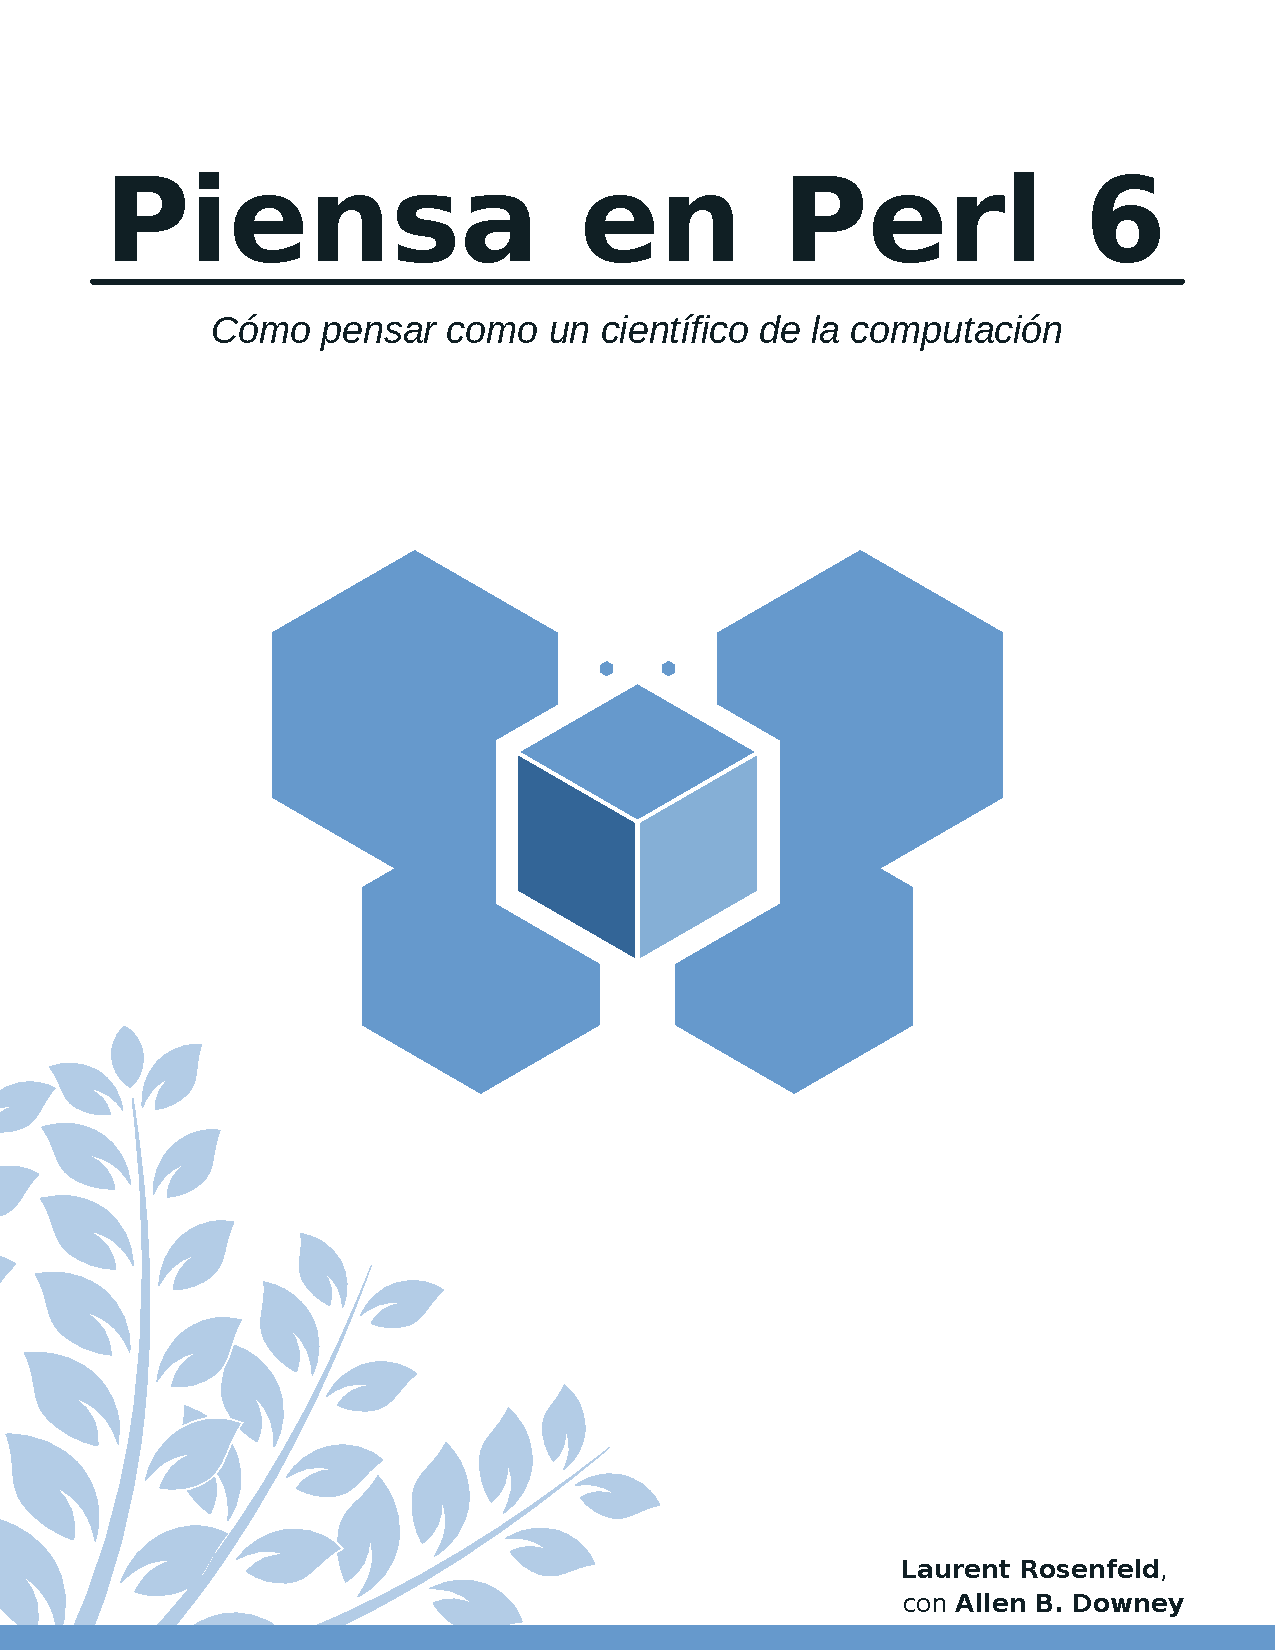
\includepdf{figs/thinkperl6_cover.pdf} 

% PLASTEX ONLY
\ifplastex
    \usepackage{localdef}
    \maketitle

\newcount\anchorcnt
\newcommand*{\Anchor}[1]{%
  \@bsphack%
    \Hy@GlobalStepCount\anchorcnt%
    \edef\@currentHref{anchor.\the\anchorcnt}% 
    \Hy@raisedlink{\hyper@anchorstart{\@currentHref}\hyper@anchorend}% 
    \M@gettitle{}\label{#1}% 
    \@esphack%
}


\else
% skip the following for plastex

\newtheorem{exercise}{Ejercicio}[chapter]

% LATEXONLY

\sloppy
%\setlength{\topmargin}{-0.375in}
%\setlength{\oddsidemargin}{0.0in}
%\setlength{\evensidemargin}{0.0in}

% Uncomment these to center on 8.5 x 11
%\setlength{\topmargin}{0.625in}
%\setlength{\oddsidemargin}{0.875in}
%\setlength{\evensidemargin}{0.875in}

%\setlength{\textheight}{7.2in}

\setlength{\headsep}{3ex}
\setlength{\parindent}{0.0in}
\setlength{\parskip}{1.7ex plus 0.5ex minus 0.5ex}
\renewcommand{\baselinestretch}{1.02}

% see LaTeX Companion page 62
\setlength{\topsep}{-0.0\parskip}
\setlength{\partopsep}{-0.5\parskip}
\setlength{\itemindent}{0.0in}
\setlength{\listparindent}{0.0in}

% see LaTeX Companion page 26
% these are copied from /usr/local/teTeX/share/texmf/tex/latex/base/book.cls
% all I changed is afterskip

\makeatletter

\renewcommand{\section}{\@startsection 
    {section} {1} {0mm}%
    {-3.5ex \@plus -1ex \@minus -.2ex}%
    {0.7ex \@plus.2ex}%
    {\normalfont\Large\bfseries}}
\renewcommand\subsection{\@startsection {subsection}{2}{0mm}%
    {-3.25ex\@plus -1ex \@minus -.2ex}%
    {0.3ex \@plus .2ex}%
    {\normalfont\large\bfseries}}
\renewcommand\subsubsection{\@startsection {subsubsection}{3}{0mm}%
    {-3.25ex\@plus -1ex \@minus -.2ex}%
    {0.3ex \@plus .2ex}%
    {\normalfont\normalsize\bfseries}}

% The following line adds a little extra space to the column
% in which the Section numbers appear in the table of contents
\renewcommand{\l@section}{\@dottedtocline{1}{1.5em}{3.0em}}
\setcounter{tocdepth}{2}

\makeatother

\newcommand{\beforefig}{\vspace{1.3\parskip}}
\newcommand{\afterfig}{\vspace{-0.2\parskip}}

\newcommand{\beforeverb}{\vspace{0.6\parskip}}
\newcommand{\afterverb}{\vspace{0.6\parskip}}

\newcommand{\adjustpage}[1]{\enlargethispage{#1\baselineskip}}


% Note: the following command seems to cause problems for Acroreader
% on Windows, so for now I am overriding it.
%\newcommand{\clearemptydoublepage}{
%            \newpage{\pagestyle{empty}\cleardoublepage}}
\newcommand{\clearemptydoublepage}{\cleardoublepage}

%\newcommand{\blankpage}{\pagestyle{empty}\vspace*{1in}\newpage}
\newcommand{\blankpage}{\vspace*{1in}\newpage}

% HEADERS

\renewcommand{\chaptermark}[1]{\markboth{#1}{}}
\renewcommand{\sectionmark}[1]{\markright{\thesection\ #1}{}}

\lhead[\fancyplain{}{\bfseries\thepage}]%
      {\fancyplain{}{\bfseries\rightmark}}
\rhead[\fancyplain{}{\bfseries\leftmark}]%
      {\fancyplain{}{\bfseries\thepage}}
\cfoot{}

\pagestyle{fancyplain}


% turn off the rule under the header
%\setlength{\headrulewidth}{0pt}

% the following is a brute-force way to prevent the headers
% from getting transformed into all-caps
\renewcommand\MakeUppercase{}

% Exercise environment
\newtheoremstyle{myex}% name
     {9pt}%      Space above
     {9pt}%      Space below
     {}%         Body font
     {}%         Indent amount (empty = no indent, \parindent = para indent)
     {\bfseries}% Thm head font
     {}%        Punctuation after thm head
     {0.5em}%     Space after thm head: " " = normal interword space;
           %       \newline = linebreak
     {}%         Thm head spec (can be left empty, meaning `normal')

\theoremstyle{myex}


\begin{latexonly}

\renewcommand{\blankpage}{\thispagestyle{empty} \quad \newpage}

%\blankpage
%\blankpage

% TITLE PAGES FOR LATEX VERSION

%-half title--------------------------------------------------
\thispagestyle{empty}

\begin{flushright}
\vspace*{2.0in}

\begin{spacing}{3}
{\huge Piensa en Perl 6}\\
{\Large Cómo Pensar Como un Científico de la Computación}
\end{spacing}

\vspace{0.25in}

\theversion

\thedate

\vfill

\end{flushright}

%--verso------------------------------------------------------

\blankpage
\blankpage
%\clearemptydoublepage
%\pagebreak
%\thispagestyle{empty}
%\vspace*{6in}

%--title page--------------------------------------------------
\pagebreak
\thispagestyle{empty}

\begin{flushright}
\vspace*{2.0in}

\begin{spacing}{3}
{\huge Piensa en Perl 6}\\
{\Large Cómo Pensar Como un Científico de la Computación}
\end{spacing}

\vspace{0.25in}

\theversion

\thedate

\vspace{1in}


{\Large
Laurent Rosenfeld,
con Allen B. Downey\\
}


\vspace{0.5in}

{\Large Green Tea Press}

{\small Needham, Massachusetts}

%\includegraphics[width=1in]{figs/logo1.pdf}
\vfill

\end{flushright}


%--copyright--------------------------------------------------
\pagebreak
\thispagestyle{empty}

{\small
Copyright \copyright ~2017 Allen Downey, Laurent Rosenfeld.


\vspace{0.2in}

\begin{flushleft}
Green Tea Press       \\
9 Washburn Ave        \\
Needham MA 02492
\end{flushleft}

Se concede permiso para copiar, distribuir y/o modificar
este documento bajo los términos de Creative Commons Attribution-NonCommercial 3.0 Unported
License, la cual está disponible en \url{http://creativecommons.org/licenses/by-nc/3.0/}.

La forma original de este libro es código fuente \LaTeX\ . La compilación de
este código \LaTeX\ tiene el efecto de generar una representación independiente
a cualquier dispositivo de este libro de texto, la cual puede ser convertida a
otros formatos e imprimida.

El código \LaTeX\ de este libro está disponible en
\url{https://github.com/LaurentRosenfeld/thinkperl6/}

\vspace{0.2in}

} % end small

\end{latexonly}


% HTMLONLY

\begin{htmlonly}

% TITLE PAGE FOR HTML VERSION

{\Large \thetitle}

{\large Laurent Rosenfeld,
con Allen B. Downey}

\theversion

\thedate

\setcounter{chapter}{-1}

\end{htmlonly}

\fi
% END OF THE PART WE SKIP FOR PLASTEX

% 
\chapter{Introducción}

Bienvenido al arte de programación de computadoras y 
al nuevo lenguaje Perl~6. Este será probablemente el primer
libro publicado que usa Perl~6 (o uno de los primeros), 
un lenguaje de programación poderoso, expresivo, maleable
y altamente extensible. Pero este libro es menos acerca de
Perl~6, y más sobre cómo aprender a escribir programas 
de computadora. 

Este libro está destinado a principiantes y no requiere ningún conocimiento
previo de programación, aunque espera que aquellos con experiencia de 
programación puedan aún así beneficiarse.

\section*{El Objetivo de este Libro}

El objetivo de este libro no es primariamente enseñar Perl~6,
sino enseñar el arte de programación, usando el lenguaje Perl~6. 
Después de haber completado el libro, con suerte deberías de ser capaz
de escribir programas para resolver problemas relativamente difíciles en 
Perl~6, pero mi objetivo principal es enseñar ciencia de la computación,
programación de software, y resolución de problemas más que solamente
enseñar el lenguaje Perl~6 por sí mismo.

Esto significa que no abarcaré cada aspecto de Perl~6, pero
solo un subconjunto (relativamente largo pero incompleto) del
lenguaje. Este libro no pretende ser una referencia del lenguaje.

No es posible aprender programación o aprender un nuevo
lenguaje de programación solo con leer un libro;
la práctica es esencial. Este libro contiene
muchos ejercicios. Se te anima a que haga un esfuerzo real
para hacerlos. Independiente a si eres capaz de resolver los 
ejercicios, deberías mirar las soluciones en el Apéndice, dado
que, muy a menudo, se sugieren varias soluciones con una extensa
discusión en la materia y los asuntos relacionados. Algunas
veces, la sección de solución del Apéndice introduce ejemplos
de temas que serán cubiertos en el siguiente capítulo---y algunas 
veces cosas que no se discutirá en otras partes del libro. Así que,
para sacarle provecho a este libro, te sugiero a que trates de solucionar
los ejercicios y revisar las soluciones e intentarlas.

Hay más de mil ejemplos de código en este libro;
estúdialos, asegúrate de entenderlos, y ejecútalos. Si es posible,
trata de cambiarlos y observa que pasa. Es probable que aprendas mucho
de este proceso.


\section*{La Historia de este Libro}

En el transcurso de los últimos tres a cuatro años,
he traducido o adaptado al francés un número de tutoriales
y artículos sobre Perl~6, y también he escrito algunos totalmente
nuevos en francés.~\footnote{Ve por ejemplo 
\url{http://perl.developpez.com/cours/\#TutorielsPerl6}.}
Juntos, estos documentos representaban para el final del 2015
entre 250 y 300 páginas de material sobre Perl~6. Para ese entonces,
probablemente había hecho público más material en francés que todos
los otros escritores juntos.

A fines del 2015, comencé a sentir un documento de Perl~6 para principiantes
era algo que faltaba que yo estaba dispuesto a llevar a cabo. Busqué alrededor
y encontré que aparentemente no existía nada igual en inglés. 
Me vino la idea que, después de todo, sería más útil escribir tal documento inicialmente
en inglés, para dárselo a una audiencia más amplia. Así fue que comencé a 
contemplar escribir una introducción para la programación de Perl~6 destinada
a principiantes. En aquel entonces, mi idea era sobre un tutorial de 50- a 70-paǵinas
y comencé a recopilar material e ideas en esta dirección.

Entonces, algo pasó que cambió mis planes.

En Diciembre del 2015, algunos amigos mío estaban contemplando
traducir al francés \emph{Think Python, Second Edition} de Allen B. Downey\footnote{Ve \url{http://greenteapress.com/wp/think-python-2e/}.}. 
Había leído una versión previa de ese libro y totalmente apoyé la idea
de traducirlo\footnote{Lo sé, es acerca de Python, no Perl.
Sin embargo, no creo en las ``guerras de lenguajes`` y pienso que todos
debemos aprender de otros lenguajes; para mí, el lema de Perl, ``hay más de 
una forma para hacer algo,`` también significa que hacerlo en Python (o cualquier
otro lenguaje) es realmente una posibilidad aceptable.}. Como resultado,
terminé como un co-traductor y el editor técnico de la traducción al francés de ese
libro\footnote{Ve
	\url{http://allen-downey.developpez.com/livres/python/pensez-python/}.}.

Mientras trabaja en la traducción al francés del libro sobre Python
de Allen, la idea se me ocurrió, en vez de escribir un tutorial
sobre Perl~6, sería más útil hacer un ``traducción a Perl~6`` de 
\emph{Think Python}. Debido a que estaba en contacto con Allen en 
el contexto de la traducción al francés, yo le sugerí la idea a Allen, 
quién acogió favorablemente la idea. Así fue como comencé a escribir este 
libro a final de Enero del 2016, poco tiempo después de haber completado
la traducción al francés de su libro sobre Python.

De tal manera, este libro es mayormente un derivado de \emph{Think Python}
de Allen, pero adaptado a Perl~6. Como sucedió, es también algo más que 
una ``traducción a Perl~6`` del libro de Allen: con suficiente nuevo material,
se ha convertido en un libro totalmente nuevo, con una gran deuda al 
libro de Allen, pero aún nuevo libro por el cual tomo toda la responsabilidad.
Cualquier error es mío, no de Allen.

Mi esperanza es que esto será útil para la comunidad de Perl~6, y
generalmente para la comunidad de código abierto (\emph{open source})
y la comunidad de la programación de computadoras. En una entrevista,
con \emph{LinuxVoice} (July 2015), Larry Wall, el creador de Perl~6, dijo:
``Nosotros pensamos que Perl 6 se podrá aprender como un primer lenguaje.``
!`Esperemos que este libro contribuya a  lograr este cometido!


\section*{Reconocimientos}

Realmente no sé cómo podría agradecerle a Larry Wall al nivel de gratitud
que él se merece por haber creado Perl en primer lugar, y 
Perl~6 más recientemente. Que seas bendecido por toda la eternidad, Larry.

Y gracias a todos ustedes que fueron parte de esta aventura (en ningún orden en 
particular), Tom, Damian, 
chromatic, Nathan, brian, Jan, Jarkko, John, Johan, Randall, 
Mark Jason, Ovid, Nick, Tim, Andy, Chip, Matt, Michael, Tatsuhiko, 
Dave, Rafael, Chris, Stevan, Saraty, Malcolm, Graham, Leon, 
Ricardo, Gurusamy, Scott y muchísimos otros.

Todas mis gracias también a aquellos quienes creyeron
en el proyecto de Perl~6 y que lo hicieron posible, incluyendo
a aquellos que abandonaron en algún momento pero que contribuyeron
por algún tiempo; sé que no fue siempre fácil.

Muchas gracias a Allen Downey, quien amablemente apoyó la idea
de adaptar su libro para Perl~6 y me ayudó en muchos aspectos,
pero también se abstuvo de interferir en lo que yo ponía en este
libro.

Le agradezco sinceramente a la gente de O'Reilly quienes 
aceptaron la idea de este libro y sugirieron muchas correcciones o 
mejoras. Quiero agradecer especialmente a Dawn Schanafelt, mi editor de 
O'Reilly, cuyos consejos han contribuido a hacer este un mejor libro.
Muchas gracias también a Charles Roumeliotis, el editor de copia, y 
Kristen Brown, la editora de producción, quien arregló muchos problemas
tipográficos y faltas ortográficas.

De antemano le doy gracias a todos los lectores quienes ofrecerán comentarios
o someterán sugerencias o correcciones, al igual que palabras de aliento.

Si ves algo que necesita ser corregido o que podría ser mejorado,
por favor amablemente envía tus comentarios a 
\url{think.perl6 (at) gmail.com}.
% ...


\section*{Lista de Contribuciones}

% ...
Me gustaría agradecer especialmente a Moritz Lenz y Elizabeth 
Mattijsen, quienes revisaron los detalles en los borradores de este 
libro y sugirieron un sin número de mejoras y correcciones.
Liz invirtió mucho tiempo en una revisión detallada del contenido
completo de este libro y le agradezco eternamente por sus numerosos
y muy útiles comentarios. Gracias también a Timo Paulssen y ryanschoppe quienes
también revisaron los primeros borradores y proveyeron algunos comentarios
útiles. Muchísimas gracias también a Uri Guttman, quien revisó este libro
y sugirió un gran número de pequeñas correcciones y mejoras un poco antes
de la publicación.  

Kamimura, James Lenz, y Jeff McClelland cada uno sometieron algunas correcciones
en la lista de errata en el sitio web de O'Reilly. zengargoyle señaló un carácter
falso en un regex y lo arregló en el repositorio Github del libro. zengargoyle
también sugirió una aclaración en el capítulo acerca de la programación
funcional. Otro James (segundo nombre que no conozco) sometió una errata
al sitio web de O'Reilly. Mikhail Korenev sugirió correcciones precisas
para tres muestras de código. Sébastien Dorey, Jean Forget, y Roland Schmitz 
enviaron algunos e-mails sugiriendo algunas correcciones o mejoras útiles. 
Luis F. Uceta señaló un error tipográfico en el texto en Github. Gil Magno 
sugirió algunas correcciones directamente en el repositorio de Github.

\clearemptydoublepage

% TABLE OF CONTENTS
\begin{latexonly}

\tableofcontents

\clearemptydoublepage

\end{latexonly}



\chapter{Introducción}

Bienvenido al arte de programación de computadoras y 
al nuevo lenguaje Perl~6. Este será probablemente el primer
libro publicado que usa Perl~6 (o uno de los primeros), 
un lenguaje de programación poderoso, expresivo, maleable
y altamente extensible. Pero este libro es menos acerca de
Perl~6, y más sobre cómo aprender a escribir programas 
de computadora. 

Este libro está destinado a principiantes y no requiere ningún conocimiento
previo de programación, aunque espera que aquellos con experiencia de 
programación puedan aún así beneficiarse.

\section*{El Objetivo de este Libro}

El objetivo de este libro no es primariamente enseñar Perl~6,
sino enseñar el arte de programación, usando el lenguaje Perl~6. 
Después de haber completado el libro, con suerte deberías de ser capaz
de escribir programas para resolver problemas relativamente difíciles en 
Perl~6, pero mi objetivo principal es enseñar ciencia de la computación,
programación de software, y resolución de problemas más que solamente
enseñar el lenguaje Perl~6 por sí mismo.

Esto significa que no abarcaré cada aspecto de Perl~6, pero
solo un subconjunto (relativamente largo pero incompleto) del
lenguaje. Este libro no pretende ser una referencia del lenguaje.

No es posible aprender programación o aprender un nuevo
lenguaje de programación solo con leer un libro;
la práctica es esencial. Este libro contiene
muchos ejercicios. Se te anima a que haga un esfuerzo real
para hacerlos. Independiente a si eres capaz de resolver los 
ejercicios, deberías mirar las soluciones en el Apéndice, dado
que, muy a menudo, se sugieren varias soluciones con una extensa
discusión en la materia y los asuntos relacionados. Algunas
veces, la sección de solución del Apéndice introduce ejemplos
de temas que serán cubiertos en el siguiente capítulo---y algunas 
veces cosas que no se discutirá en otras partes del libro. Así que,
para sacarle provecho a este libro, te sugiero a que trates de solucionar
los ejercicios y revisar las soluciones e intentarlas.

Hay más de mil ejemplos de código en este libro;
estúdialos, asegúrate de entenderlos, y ejecútalos. Si es posible,
trata de cambiarlos y observa que pasa. Es probable que aprendas mucho
de este proceso.


\section*{La Historia de este Libro}

En el transcurso de los últimos tres a cuatro años,
he traducido o adaptado al francés un número de tutoriales
y artículos sobre Perl~6, y también he escrito algunos totalmente
nuevos en francés.~\footnote{Ve por ejemplo 
\url{http://perl.developpez.com/cours/\#TutorielsPerl6}.}
Juntos, estos documentos representaban para el final del 2015
entre 250 y 300 páginas de material sobre Perl~6. Para ese entonces,
probablemente había hecho público más material en francés que todos
los otros escritores juntos.

A fines del 2015, comencé a sentir un documento de Perl~6 para principiantes
era algo que faltaba que yo estaba dispuesto a llevar a cabo. Busqué alrededor
y encontré que aparentemente no existía nada igual en inglés. 
Me vino la idea que, después de todo, sería más útil escribir tal documento inicialmente
en inglés, para dárselo a una audiencia más amplia. Así fue que comencé a 
contemplar escribir una introducción para la programación de Perl~6 destinada
a principiantes. En aquel entonces, mi idea era sobre un tutorial de 50- a 70-paǵinas
y comencé a recopilar material e ideas en esta dirección.

Entonces, algo pasó que cambió mis planes.

En Diciembre del 2015, algunos amigos mío estaban contemplando
traducir al francés \emph{Think Python, Second Edition} de Allen B. Downey\footnote{Ve \url{http://greenteapress.com/wp/think-python-2e/}.}. 
Había leído una versión previa de ese libro y totalmente apoyé la idea
de traducirlo\footnote{Lo sé, es acerca de Python, no Perl.
Sin embargo, no creo en las ``guerras de lenguajes`` y pienso que todos
debemos aprender de otros lenguajes; para mí, el lema de Perl, ``hay más de 
una forma para hacer algo,`` también significa que hacerlo en Python (o cualquier
otro lenguaje) es realmente una posibilidad aceptable.}. Como resultado,
terminé como un co-traductor y el editor técnico de la traducción al francés de ese
libro\footnote{Ve
	\url{http://allen-downey.developpez.com/livres/python/pensez-python/}.}.

Mientras trabaja en la traducción al francés del libro sobre Python
de Allen, la idea se me ocurrió, en vez de escribir un tutorial
sobre Perl~6, sería más útil hacer un ``traducción a Perl~6`` de 
\emph{Think Python}. Debido a que estaba en contacto con Allen en 
el contexto de la traducción al francés, yo le sugerí la idea a Allen, 
quién acogió favorablemente la idea. Así fue como comencé a escribir este 
libro a final de Enero del 2016, poco tiempo después de haber completado
la traducción al francés de su libro sobre Python.

De tal manera, este libro es mayormente un derivado de \emph{Think Python}
de Allen, pero adaptado a Perl~6. Como sucedió, es también algo más que 
una ``traducción a Perl~6`` del libro de Allen: con suficiente nuevo material,
se ha convertido en un libro totalmente nuevo, con una gran deuda al 
libro de Allen, pero aún nuevo libro por el cual tomo toda la responsabilidad.
Cualquier error es mío, no de Allen.

Mi esperanza es que esto será útil para la comunidad de Perl~6, y
generalmente para la comunidad de código abierto (\emph{open source})
y la comunidad de la programación de computadoras. En una entrevista,
con \emph{LinuxVoice} (July 2015), Larry Wall, el creador de Perl~6, dijo:
``Nosotros pensamos que Perl 6 se podrá aprender como un primer lenguaje.``
!`Esperemos que este libro contribuya a  lograr este cometido!


\section*{Reconocimientos}

Realmente no sé cómo podría agradecerle a Larry Wall al nivel de gratitud
que él se merece por haber creado Perl en primer lugar, y 
Perl~6 más recientemente. Que seas bendecido por toda la eternidad, Larry.

Y gracias a todos ustedes que fueron parte de esta aventura (en ningún orden en 
particular), Tom, Damian, 
chromatic, Nathan, brian, Jan, Jarkko, John, Johan, Randall, 
Mark Jason, Ovid, Nick, Tim, Andy, Chip, Matt, Michael, Tatsuhiko, 
Dave, Rafael, Chris, Stevan, Saraty, Malcolm, Graham, Leon, 
Ricardo, Gurusamy, Scott y muchísimos otros.

Todas mis gracias también a aquellos quienes creyeron
en el proyecto de Perl~6 y que lo hicieron posible, incluyendo
a aquellos que abandonaron en algún momento pero que contribuyeron
por algún tiempo; sé que no fue siempre fácil.

Muchas gracias a Allen Downey, quien amablemente apoyó la idea
de adaptar su libro para Perl~6 y me ayudó en muchos aspectos,
pero también se abstuvo de interferir en lo que yo ponía en este
libro.

Le agradezco sinceramente a la gente de O'Reilly quienes 
aceptaron la idea de este libro y sugirieron muchas correcciones o 
mejoras. Quiero agradecer especialmente a Dawn Schanafelt, mi editor de 
O'Reilly, cuyos consejos han contribuido a hacer este un mejor libro.
Muchas gracias también a Charles Roumeliotis, el editor de copia, y 
Kristen Brown, la editora de producción, quien arregló muchos problemas
tipográficos y faltas ortográficas.

De antemano le doy gracias a todos los lectores quienes ofrecerán comentarios
o someterán sugerencias o correcciones, al igual que palabras de aliento.

Si ves algo que necesita ser corregido o que podría ser mejorado,
por favor amablemente envía tus comentarios a 
\url{think.perl6 (at) gmail.com}.
% ...


\section*{Lista de Contribuciones}

% ...
Me gustaría agradecer especialmente a Moritz Lenz y Elizabeth 
Mattijsen, quienes revisaron los detalles en los borradores de este 
libro y sugirieron un sin número de mejoras y correcciones.
Liz invirtió mucho tiempo en una revisión detallada del contenido
completo de este libro y le agradezco eternamente por sus numerosos
y muy útiles comentarios. Gracias también a Timo Paulssen y ryanschoppe quienes
también revisaron los primeros borradores y proveyeron algunos comentarios
útiles. Muchísimas gracias también a Uri Guttman, quien revisó este libro
y sugirió un gran número de pequeñas correcciones y mejoras un poco antes
de la publicación.  

Kamimura, James Lenz, y Jeff McClelland cada uno sometieron algunas correcciones
en la lista de errata en el sitio web de O'Reilly. zengargoyle señaló un carácter
falso en un regex y lo arregló en el repositorio Github del libro. zengargoyle
también sugirió una aclaración en el capítulo acerca de la programación
funcional. Otro James (segundo nombre que no conozco) sometió una errata
al sitio web de O'Reilly. Mikhail Korenev sugirió correcciones precisas
para tres muestras de código. Sébastien Dorey, Jean Forget, y Roland Schmitz 
enviaron algunos e-mails sugiriendo algunas correcciones o mejoras útiles. 
Luis F. Uceta señaló un error tipográfico en el texto en Github. Gil Magno 
sugirió algunas correcciones directamente en el repositorio de Github.

\clearemptydoublepage

% TABLE OF CONTENTS
\begin{latexonly}

\tableofcontents

\clearemptydoublepage

\end{latexonly}



% START THE BOOK
\mainmatter

\part{Comenzando con lo Básico}

% intro_part_1.tex -- Introduction to first part of the book
%

Este libro está dividido en dos partes. La razón principal 
por esta decisión es que yo quería hacer una distinción entre 
las nociones relativamente básicas que cualquier programador necesita 
al usar Perl~6 y los conceptos avanzados que un buen programador
necesita saber y que pueden ser necesarios en el día a día de un programador.

Los primeros once capítulos (aproximadamente 200 páginas) 
que constituyen la primera parte están diseñados para enseñar los
conceptos básicos que cada programador debe conocer: variables,
expresiones, condiciones, recursión, precedencia de operadores, bucles,
etc., y también las estructuras de datos básicas usadas comúnmente, 
y los algoritmos más útiles. Creo que estos capítulos pueden
ser la base de un curso introductorio a la programación
de un semestre.
 
Por supuesto, el profesor o instructor que desee utilizar este material
es libre de saltar algunos detalles en la Parte~1 (y también incluir 
de la Parte~2). Por lo menos, he incluido algunas recomendaciones
sobre como este libro podría ser usado para enseñar programación
usando el lenguaje Perl~6.

La segunda parte se enfocan en paradigmas diferentes y algunas
técnicas avanzadas de programación que son en mi opinión de gran
importancia, pero que deberían ser estudiados en el contexto
de un segundo semestre más avanzado.

Por ahora, comencemos con lo básico. Espero que disfrute la travesía.



\chapter{La Forma del Programa}

La meta de este libro es enseñarte a pensar como un científico de la 
computación. Esta manera de pensar combina algunas de las mejores características
de las matemáticas, la ingeniería, y las ciencias naturales. Al igual que los
matemáticos, los científicos de la computación usan lenguajes formales para denotar
ideas (específicamente computaciones). Al igual que los ingenieros, ellos diseñan cosas,
ensamblan componentes en sistemas y evalúan las compensaciones entre las alternativas.
Al igual que los científicos, ellos observan el comportamiento de sistemas complejos, 
formulan hipótesis, y prueban las predicciones. 
\index{problem solving}
\index{formal language}

La habilidad más importante de un científico de la computación
es la {\bf resolución de problemas}. La resolución de problemas se refiere
a la habilidad de formular problemas, pensar creativamente sobre las
soluciones, y expresar una solución clara y precisamente. Como sucede, 
el proceso de aprender a programar es una oportunidad excelente para practicar 
las habilidades de resolución de problemas. Por esta razón, este capítulo se titula,
 ``La Forma del Programa.``

En un nivel, aprenderás a programar, la cual es una habilidad útil por sí misma.
En otro nivel, aprenderás a usar la programación como un medio para un fin. 
A medida que avancemos, este fin se volverá más claro.
\index{programming}


\section{?`Qué es un Programa?}

Un {\bf programa} es una secuencia de instrucciones que especifica
como realizar una computación. La computación podría involucrar 
algo matemático, tal como resolver un sistema de ecuaciones o 
encontrar las raíces de un polinomio, pero también puede ser algo
simbólico, tal como buscar y reemplazar texto en un documento, o 
algo gráfico, como el procesamiento de una imagen o la reproducción 
de un video.
\index{program}

Los detalles lucen diferentes en lenguajes distintos, pero hay algunas
instrucciones básicas que aparecen en casi todos los lenguajes:

\begin{description}

\item[Entrada] Obtener datos desde el teclado, un archivo, la red, 
un sensor, un chip de GPS o algún otro dispositivo.
\index{input}

\item[Salida] Mostrar información en la pantalla, guardarla en un archivo,
 enviarla a través de la red, actuar en un dispositivo mecánico,  etc.
\index{output}

\item[Matemática] Realizar operaciones matemáticas básicas tales como la adición y
la multiplicación.

\item[Ejecución condicional] Revisar ciertas condiciones y ejecutar el código 
apropiadamente.
\index{conditional!execution}

\item[Repetición] Realizar alguna acción repetidamente, usualmente con alguna
forma de variación.
\index{repetition}

\end{description}

Lo creas o no, eso es todo. Cada programa que has usado, sin importar
que tan complicado sea, está compuesto de instrucciones que lucen exactamente
como estas. Por lo tanto, puedes imaginarte la programación como el 
proceso de fragmentar una tarea grande y compleja en piezas más pequeñas
las cuales se pueden ejecutar con una de estas operaciones básicas.
\index{instruction}

\index{abstraction}
\index{subtask}
Al usar o llamar estas piezas, es posible crear varios niveles
de \emph{abstracción}. Probablemente te han dicho que las computadoras
solamente usan 0s y 1s al nivel más fundamental; pero usualmente no 
nos preocupamos acerca de esto. Cuando usamos un procesador de texto para
escribir una carta o un reporte, estamos interesados en archivos con textos
y algunas instrucciones de formato, y con comandos para cambiar el archivo o
imprimirlo; afortunadamente, no tenemos que preocuparnos sobre los 0s y 1s; el
procesador de texto nos ofrecemos una vista más general (archivos, comandos, etc,)
que oculta todos los detalles insignificantes para el usuario. 


Similarmente, cuando escribimos un programa, 
usualmente usamos y/o creamos varias capas de abstracción, 
para que, por ejemplo, una vez que hayamos creado una tarea pequeña 
que consulta una base de datos y guarda la información relevante
en la memoria, no tenemos que preocuparnos sobre los detalles técnicos
de la tarea. Podemos usarla como una caja negra la cual realizará 
la operación deseada para nosotros. La esencia de la programación es 
en gran parte este arte de crear estas capas sucesivas de abstracción 
de tal manera que realizar tareas de niveles más altos se vuelva 
relativamente más fácil.
\index{subtask}
\index{black box}


\section{Ejecutando Perl~6}
\label{running_perl_6}

Uno de los retos de comenzar con Perl~6 es que podrías tener que instalar
Perl~6 y cualquier software relacionado en tu computadora. Si estás familiarizado
con tu sistema operativo, y especialmente te sientes cómodo con shell o
intérprete de comandos, no tendrás problemas instalando Perl~6. Para los 
principiantes, puede ser un poco difícil aprender sobre la
administración de sistema y programación al mismo tiempo.

Para evitar ese problema, podrías comenzar ejecutando Perl~6 en
el navegador. Podrías usar un motor de búsquedas para encontrar tal
sitio. Por el momento, la forma más fácil es probablemente conectarse
al sitio \url{https://glot.io/new/perl6}, donde puedes escribir código
de Perl~6 en la ventana principal, ejecutarlo, y observar el resultado 
en la ventana de salida más abajo.
\index{Perl~6 in a browser}

Tarde o temprano, sin embargo, tendrás que instalar Perl~6 en tu computadora.

La manera más fácil de instalar Perl~6 en tu sistema es descargar 
Rakudo Star (una distribución de Perl~6 que contiene el {\bf compilador}
Rakudo de Perl~6, documentación y módulos útiles): sigue las instrucciones 
para tu sistema operativo en
\url{http://rakudo.org/how-to-get-rakudo/} y en 
\url{https://perl6.org/downloads/}. 

\index{Perl 6 version}
Al momento de escribir este libro, la especificación más reciente del 
lenguaje es Perl~6 version 6c (v6.c), y el lanzamiento más reciente disponible
para la descarga es Rakudo Star 2016.07; los ejemplos en este libro deberían
funcionar con esta versión. Puedes encontrar la versión instalada al ejecutar
el siguiente comando en el intérprete de comandos de tu sistema operativo:
\begin{verbatim}
$ perl6 -v
This is Rakudo version 2016.07.1 built on MoarVM version 2016.07
implementing Perl 6.c.
\end{verbatim}

No obstante, deberías descargar e instalar las versión más reciente que puedas
encontrar. La salida (advertencias, mensajes de errores, etc.) que obtendrás de tu versión de Perl
podría en algunos casos diferir de la que se encuentra en este libro, pero estas diferencias
deberían ser esencialmente cosméticas.

Comparado con Perl~5, Perl~6 no es sólo una nueva versión de Perl.
Es como la nueva hermana menor de Perl~5. Su objetivo no es reemplazar
a Perl~5. Perl~6 es realmente un nuevo lenguaje de programación, con una sintaxis
que es similar a las versiones anteriores de Perl (tal como Perl~5), pero considerablemente
diferente. Al menos que se indique lo contrario, este libro es sobre Perl~6 solamente, no
acerca de Perl~5 y versiones anteriores del lenguaje de programación Perl. Desde aquí adelante,
cuando hablemos de \emph{Perl} sin ninguna cualificación, nos referimos a Perl~6.


El {\bf interpretador} de Perl~6 es un programa que lee y  
ejecuta código de Perl~6. Algunas veces se le llama REPL (por ``read, 
evaluate, print, loop''). Dependiendo de tu entorno, 
podría iniciar el interpretador al cliquear un ícono, o al 
escribir {\tt perl6} en el intérprete de comandos.

Cuando comience, deberías ver algo similar a esto:
\index{interpreter}
\index{REPL}

\begin{verbatim}
To exit type 'exit' or '^D'
(Possibly some information about Perl and related software)
> 
\end{verbatim}
%

La última línea con {\tt >} es un {\bf prompt} que indica 
que el REPL está listo para que entres código. Si escribes un 
línea de código y presiona Enter, el interpretador muestra el resultado: 
\index{prompt}

\begin{lstlisting}
> 1 + 1
2
>
\end{lstlisting}
%
Puedes escribir {\tt exit} en el prompt de REPL para salir del REPL.

Ahora estás listo para comenzar.
De aquí en adelante, asumimos que sabes como iniciar el REPL de Perl~6 y 
ejecutar código.


\section{El Primer Programa}
\label{hello}
\index{Hello, World}

Tradicionalmente, el primer programa que escribes en un nuevo lenguaje
se llama ``Hello, World'' porque todo lo que hace es mostrar las palabras
``Hello, World.''  En Perl~6, luce de la siguiente manera:

\begin{lstlisting}
> say "Hello, World";
Hello, World
>
\end{lstlisting}
%
\index{say function or method}
\index{function!say}
Este es un ejemplo de lo que usualmente se conoce como una {\bf sentencia de impresión},
aunque actualmente no imprime nada sobre el papel y ni siquiera usa la palabra clave
{\tt print} 
\footnote{Perl también tiene una función {\tt print},
pero la función integrada {\tt say} es usada aquí 
porque agrega un carácter de nueva línea a la salida.}
(palabras claves son palabras que tienen un significado especial
en el lenguaje y son usadas por el interpretador para reconocer la
estructura del programa).
La sentencia print muestra un resultado en la pantalla. En este caso, 
el resultado son las palabra {\tt Hello World}.
%
Las comillas inglesas en el programa indican el comienzo y final
del texto a ser mostrado; ellas no aparecen en el resultado.
\index{quotation mark}
\index{print statement}
\index{statement!print}

El punto y medio ``{\tt ;}'' al final de la línea indica
que este es el final de la sentencia actual. Aunque un punto y medio
no es técnicamente necesario al ejecutar código simple en el REPL, 
es usualmente necesario cuando se escribe un programa con varias líneas
de código, así que podrías ir acostumbrándote a finalizar instrucciones
de código con un punto y medio.   
\index{semi-colon}

Otros lenguajes de programación podrían requerir paréntesis
alrededor de la oración que se quiere mostrar, pero esto es usualmente 
no necesario en Perl~6.

\section{Operadores Aritméticos}
\index{operator!arithmetic}
\index{arithmetic operator}

Después de ``Hello, World,'' el siguiente paso es aritmética. Perl~6 provee {\bf operadores}, los cuales son símbolos especiales que representan computaciones tales como adición y multiplicación.

Los operadores {\tt +}, {\tt -}, {\tt *}, y {\tt /} realizan adición,, sustracción, multiplicación y división, como en los siguientes ejemplos en el REPL:

\begin{lstlisting}
> 40 + 2
42
> 43 - 1
42
> 6 * 7
42
> 84 / 2
42
\end{lstlisting}
%

Dado que usamos el REPL, no necesitamos una sentencia print explícita
en estos ejemplos, debido a que el REPL automáticamente imprime el resultado de las sentencias. En un programa real, necesitarías una sentencia print para mostrar el resultado, como veremos más adelante. Similarmente, si ejecutas sentencias de Perl en el navegador mencionado en la sección~\ref{running_perl_6}, necesitarás una sentencia print para mostrar el resultado de estas operaciones.
Por ejemplo:

\begin{lstlisting}
say 40 + 2;   # -> 42
\end{lstlisting}


Finalmente, el operador {\tt **} realiza potenciación; es decir que eleva un número a un exponente:

\begin{lstlisting}
> 6**2 + 6
42
\end{lstlisting}
%
En otros lenguages, el signo de intercalación (``\verb"^"'') o el acento circunflejo es usado para la potenciación, pero en Perl~6 se utiliza para otros propósitos.
%
\index{set}
\index{set!operator}
\index{operator!set}


\section{Valores y Tipos}
\label{values_and_types}
\index{value}
\index{type}
\index{string}

Un {\bf valor} es una de las cosas básicas con la cual un programa funciona,
como una letra o un número. Entre algunos de los valores que hemos visto hasta ahora
están {\tt 2}, {\tt 42}, y \verb'"Hello, World"'.

Estos valores pertenecen a diferentes {\bf tipos}: 
{\tt 2} es un número {\bf entero}, {\tt 40 + 2} es también un entero, 
{\tt 84/2} es un número {\bf racional}, y  \verb"'Hello, World'" es una
{\bf cadena de texto}, llamada así porque los caracteres que contiene están
unidos juntos.
\index{integer}
\index{floating-point}

Si no estás seguro del tipo que un valor tiene, Perl puede decirte:

\begin{lstlisting}
> say 42.WHAT;
(Int)
> say (40 + 2).WHAT;
(Int)
> say (84 / 2).WHAT;
(Rat)
> say (42.0).WHAT
(Rat)
> say ("Hello, World").WHAT;
(Str)
>
\end{lstlisting}
%
En estas instrucciones, a {\tt .WHAT} se le conoce como un método 
de introspección, el cual es un tipo de método que te dice de \emph{que}
tipo la expresión precedente es. {\tt 42.WHAT} es un ejemplo de la sintaxis 
del punto usada para la invocación de método: invoca el método integrado
{\tt .WHAT} sobre la expresión ``42'' (el invocante) y provee la función {\tt say}
con el resultado de esta invocación, que en este caso es el tipo de la expresión.
\index{WHAT}
\index{introspection}
\index{string!type}
\index{type!Str}
\index{Int type}
\index{type!Int}
\index{rational!type}
\index{type!Rat}
\index{invocant}
\index{invocation}

No resulta sorprendente que los números enteros pertenecen al tipo
{\tt Int}, las cadenas de texto pertenecen a {\tt Str}, y los números racionales
pertenecen a {\tt Rat}. 

Aunque {\tt 40 + 2} y {\tt 84 / 2} parecen arrojar el mismo resultado (42),
la primera expresión devuelve un entero ({\bf Int}), y la segunda devuelve
un número racional ({\bf Rat}). El número 42.0 es también un número racional.

El tipo racional no es algo muy común en la mayoría de lenguajes de programación.
Internamente, estos números se almacenan como dos enteros los cuales representan
el numerador y el denominador (en sus términos más simples). Por ejemplo, el número
17.3 podría ser almacenado como dos enteros, 173 y 10, lo cual significa que
Perl está realmente almacenando la fracción $\frac{173}{10}$. Aunque esto no es 
usualmente soportado (excepto para introspección o depuración), puedes accesar estos
dos enteros con los métodos siguientes:

\begin{lstlisting}
> my $num = 17.3;
17.3
> say $num.WHAT;
(Rat)
> say $num.numerator, " ", $num.denominator; # say puede imprimir una lista
173 10
> say $num.nude;      # "nude" significa (nu)merator-(de)nominator
(173 10) 
\end{lstlisting}
\index{numerator method}
\index{method!numerator}
\index{denominator method}
\index{method!denominator}
\index{nude method}
\index{method!nude}
%
Esto puede parecer anecdótico, pero por razones más allá del
ámbito de este libro, esto permite que Perl~6 pueda llevar a cabo 
operaciones aritméticas sobre números racionales con un nivel 
de precisión mucho mayor que en los lenguajes de programación más comunes.
Por ejemplo, si intentas llevar a cabo la siguiente operación aritmética 
\verb'0.3 - 0.2 - 0.1', con los lenguajes de programación más generales 
(y dependiendo en la arquitectura de tu máquina), podrías obtener un resultado
tal como -2.77555756156289e-17 (en Perl~5), 
-2.775558e-17 (en C con gcc), o -2.7755575615628914e-17 
(Java, Python~3, Ruby, TCL). No te preocupe acerca de estos valores si no
los entiendes, digamos que son extremadamente pequeños, pero no son 0,
mientras que, obviamente, el resultado debería ser realmente cero. En 
Perl~6, el resultado es 0 (hasta el quinceavo dígito decimal):
\begin{lstlisting}
> my $result-should-be-zero = 0.3 - 0.2 - 0.1;
0
> printf "%.50f", $result-should-be-zero; # imprime 50 dígitos decimales
0.00000000000000000000000000000000000000000000000000
\end{lstlisting}
%
En Perl~6, podrías hasta comparar el resultado de la operación con 0:
\begin{lstlisting}
> say $result-should-be-zero == 0;
True
\end{lstlisting}
%
No hagas tal comparación con los lenguajes de programación más comunes;
es posible que obtengas un resultado erróneo.

?`Qué acerca de valores como \verb'"2"' y \verb'"42.0"'?
Ellos parecen números, pero están en comillas inglesas como las 
cadenas de texto.
\index{quotation mark}

\begin{lstlisting}
> say '2'.perl; # perl devuelve una representación de Perl del invocante
"2"
> say "2".WHAT;
(Str)
> say '42'.WHAT;
(Str)
\end{lstlisting}
%
\index{invocant}

Ellos son cadenas de texto porque están definidos dentro de comillas inglesas.
Aunque Perl usualmente realizará las conversiones necesarias para ti, es generalmente
buena práctica no usar comillas inglesas si tu valor está supuesto a ser un
número.

Cuando escribes un número entero largo, podrías estar tentado a usar comas
entre grupos de dígitos, como en {\tt 1,234,567}. Esto no es un {\em entero}
legal en Perl~6, pero sí es una expresión legal:

\begin{lstlisting}
> 1,234,567
(1 234 567)
>
\end{lstlisting}
%
!`Eso es actualmente una lista de tres números enteros diferentes, 
y no lo que esperábamos! 

\begin{lstlisting}
> say (1,234,567).WHAT
(List)
\end{lstlisting}

Perl~6 interpreta {\tt 1,234,567} como una secuencia de tres números enteros
separados por coma. Como veremos más adelante, la coma es un separador usado
para construir listas.
\index{comma}

No obstante, puedes separar grupos de dígitos con una barra baja ``\verb"_"''
para mejorar la legibilidad y para obtener un entero propio:
\index{underscore character}

\begin{lstlisting}
> 1_234_567
1234567
> say 1_234_567.WHAT
(Int)
>
\end{lstlisting}
%

\index{sequence}



\section{Lenguajes Formales y Naturales}
\index{formal language}
\index{natural language}
\index{language!formal}
\index{language!natural}

Los {\bf lenguajes naturales} son los lenguajes que las personas hablan,
como el inglés, el español y el francés.  Ellos no fueron diseñados por personas
(aunque la gente trata de imponer cierto orden sobre ellos); ellos evolucionaron
naturalmente.

Los {\bf lenguajes formales} son lenguajes que son diseñados por personas
para aplicaciones específicas. Por ejemplo, la notación que los matemáticos 
utilizan es un lenguaje formal que es particularmente buena para denotar relaciones
entre números y símbolos. Los químicos usan un lenguaje formal para representar
la estructura química de las moléculas. Y más importante:

\begin{quote}
{\bf Los lenguajes de programación son lenguajes formales que han sido diseñados
para expresar computaciones.}
\end{quote}

Los lenguajes formales tienen usualmente {\bf reglas sintácticas} estrictas
que gobiernan la estructura de las sentencias. Por ejemplo, en matemáticas la
sentencia $3 + 3 = 6$ es sintácticamente correcta pero $3 + = 3 \$ 6$ no lo es.
En química  $H_2O$ es una fórmula sintácticamente correcta, pero $_2Zz$ no lo es.
\index{syntax}

Las reglas sintácticas vienen en dos formas, pertenecientes a los {\bf tókenes} 
y la {\bf estructura}. Los tókenes son los elementos básicos del lenguaje, 
tales como las palabras, números, y elementos químicos. Uno de los problemas
con $3 += 3 \$ 6$ es que \( \$ \) no es un token legal en matemáticas (
al menos eso es lo que sé).  Similarmente, $_2Zz$ no es legal porque
no hay elemento químico con la abreviación $Zz$.
\index{token}
\index{structure}

La estructura es el segundo tipo de la regla sintáctica, la cual
se concierne con la forma en que los tókenes son combinados. La ecuación
$3 += 3$  es ilegal en matemáticas porque, aunque $+$ y $=$ son 
tókenes legales, no puedes tenerlos uno detrás del otro. De manera similar,
en una fórmula química, el subíndice que representa el número de átomos en un
compuesto químico viene después del nombre del elemento, no antes.

% Instead of using the original sentence in English,
% I translated it to Spanish (using Spanish as the base language) so that the speaker has a better
% understanding of the difference between tokens and structure.
Esto es un@ oración en español bien e\$tructurada con t*kenes
inválidos. En esta oración todos tókenes los válidos son, pero la
inválida estructura es.

Cuando lees una oración en español o una sentencia en un lenguaje
formal, debes descifrar la estructura (aunque en en un lenguaje natural
lo haces inconscientemente). Este proceso es conocido como {\bf análisis 
sintáctico} ({\em parsing} en inglés).
\index{parse}

Aunque los lenguajes formales y naturales comparten muchas características en común
---tókenes, estructura, y sintaxis---también hay algunas diferencias:
\index{ambiguity}
\index{redundancy}
\index{literalness}

\begin{description}

\item[Ambigüedad] Los lenguajes naturales están llenos de ambigüedades,
y las personas lidian con ellas a través del uso de contexto y cualquier
información adicional. Los lenguajes formales son diseñados para no tener
ambigüedades, de tal manera que cualquier oración tiene exactamente un solo
significado.

\item[Redundancia] Para compensar por las ambigüedades y reducir los malentendidos
, los lenguajes naturales hacen uso de muchas redundancias. Como resultado,
ellos tienden a ser verbosos. En cambio, los lenguajes formales son menos
redundantes y más concisos.

\item[Literalidad] Los lenguajes naturales están llenos de modismos
y metáforas. Si decimos, ``Hablar por los codos,`` es probable que nadie
está hablando por los codos literalmente (este modismo significa que una persona
habla demasiado). Los lenguajes formales hacen referencias exactas a lo que quieren
decir.

\end{description}

Debido a que todos crecemos hablando lenguajes naturales, es un poco 
difícil ajustarse a los lenguajes formales. La diferencia entre un lenguaje formal
y un lenguaje natural es como la diferencia entre la poesía y la prosa, pero
más definida: \index{poetry} \index{prose}

\begin{description}

\item[Poesía] La palabras son usadas tanto pos sus sonidos como
sus significados, y el poema completo crea un efecto o respuesta
emocional. En este caso, la ambigüedad no es solo común sino usualmente
deliberada. 

\item[Prosa] El significado literal de las palabras es más importante, y la estructura
contribuye más al significado. La prosa es más amena para el análisis que la poesía
aunque es muchas veces aún ambigua.

\item[Programas] El significado de un programa de computadora es literal y 
no tiene ambigüedades. Dicho programa puede ser comprendido enteramente a través
del análisis de los tókenes y la estructura.

\end{description}

Los lenguajes formales son mucho más densos que los lenguajes naturales,
y por lo tanto se tarda más en leerlos. De igual manera, la estructura
es importante y algunas veces, no siempre es eficiente leerlos de arriba
hacia abajo o de izquierda a derecha. Por lo contrario, mejor aprende
a parsear el programa en tu cabeza, identificando los tókenes e interpretando
la estructura. Finalmente, los detalles importan. Pequeños errores en 
la ortografía y la puntuación que no son de mucha importancia en los 
lenguajes naturales, pueden hacer una gran diferencia en un lenguaje formal.


\section{Depuración de Programas}
\index{debugging}

Los programadores cometen errores. A los errores de programación 
se les conoce usualmente como {\bf bichos} ({\em bugs}) y el proceso 
de eliminación de estos errores se llama {\bf depuración de programas} 
({\em debugging}).
\index{debugging}
\index{bug}

La programación, y especialmente la depuración de programas, algunas veces
puede aflorar emociones fuertes. Si estás batallando con un error difícil, podrías
sentirte enojada/o, avergonzada/o o desanimada/o.

Existe evidencia que sugiere que las personas responden naturalmente
a las computadoras como si fueran personas. Cuando funcionan adecuadamente,
las consideramos nuestras compañeras, y cuando son obstinadas y groseras, 
nosotros nos dirigimos hacia ellas de la misma manera que lo 
haríamos con personas obstinadas y groseras\footnote{Reeves and Nass, {\it The Media
    Equation: How People Treat Computers, Television, and New Media
    Like Real People and Places}, (Center for the Study of Language and Information, 2003).)}.
\index{debugging!emotional response}
\index{emotional debugging}

Prepararse de antemanos para lidiar con estas reacciones
puede ser beneficioso. Una estrategia es tratar de pensar acerca
de la computadora como si fuera un empleado con ciertas fortalezas,
como la velocidad y la precisión, y con debilidades particulares 
tales como la falta de empatía y la inhabilidad para comprender
la perspectiva general.

Tu trabajo es ser un buen gerente: encuentra maneras de tomar
ventaja de las fortalezas y mitigar las debilidades. Y encontrar maneras
de usar tus emociones para familiarizarte y envolverte con el problema
sin dejar que tus reacciones interfieran con tu habilidad de trabajar 
efectivamente. 

Aprender a depurar puede ser frustrante, pero es una habilidad valiosa
que será muy útil para muchas actividades más allá de la programación. 
Al final de cada capítulo hay una sección, como esta, con sugerencias para la
depuración. !`Espero que sean útiles!


\section{Glosario}

\begin{description}

\item[Resolución de problemas]  El proceso de formular un problema, 
encontrar una solución y expresarla adecuadamente.
\index{problem solving}

\item[Abstracción] Una manera de proveer una perspectiva de alto nivel
de una tarea y ocultar los detalles técnicos con el propósito de hacer 
la tarea más simple.

\item[Interpretador]  Un programa que lee otro programa y lo ejecuta.
\index{interpret}

\item[Compilador]  Un programa que lee otro programa y lo transforma en código ejecutable
de computadora; solía ser que había una gran diferencia entre lenguajes
interpretados y lenguajes compilados, sin embargo esta distinción se ha vuelto
más difusa en las últimas dos décadas.
\index{compiler}

\item[Prompt] El interpretador muestra caracteres en la pantalla para indicar 
que está listo para recibir entrada de texto por el usuario.
\index{prompt}

\item[Program] Un conjunto de instrucciones que especifica una computación.
\index{program}

\item[Sentencia print]  Una instrucción que causa que el interpretador de Perl~6
muestre un valor en la pantalla. 
\index{print statement}
\index{statement!print}

\item[Operador]  Un símbolo especial que representa una simple computación como
adición, multiplicación, o la concatenación de una cadena de texto.
\index{operator}

\item[Valor]  Una de las unidades básicas de dato, como un número o una
cadena de texto, que un programa manipula.
\index{value}

\item[Tipo] Una categoría de valores. Los tipos que hemos visto hasta
ahora son números enteros (tipo {\tt Int}), números racionales (tipo {\tt Rat}),
y cadenas de texto (tipo {\tt Str}).
\index{type}

\item[Entero] Un tipo que representa valores enteros.
\index{integer}

\item[Racional] Un tipo que representa números con partes fraccionales. 
Internamente, Perl almacena un racional como dos números enteros
que representan respectivamente el numerador y denominador de una 
fracción.
\index{rational}

\item[Cadena de texto] Un tipo que representa secuencias de caracteres.
\index{string}

\item[Lenguaje natural]  Cualquiera de los lenguajes que las 
personas hablan y que han evolucionado naturalmente.
\index{natural language}

\item[Lenguaje formal]  Cualquiera de los lenguajes que las personas
han diseñado para propósitos específicos tales como la representación de 
ideas matemáticas o programas de computadoras; todos los lenguajes de programación
son lenguajes formales.
\index{formal language}

\item[Token]  Uno de los elementos básicos de la estructura sintáctica de 
un programa. El concepto es análogo a una palabra en un lenguaje natural.
\index{token}

\item[Sintaxis] Las reglas que dictan la estructura de un programa.
\index{syntax}

\item[Análisis sintáctico] Examinar un programa y analizar su estructura sintáctica.
\index{parse}

\item[Bicho] Un error en un programa.
\index{bug}

\item[Depuración] El proceso por el cual se encuentran y corrigen errores de programación.
\index{debugging}

\end{description}


\section{Ejercicios}

\begin{exercise}

Es una buena idea que lea este libro al frente de una computadora
para que puedas intentar los ejemplos según avanzas. 

Cuando experimentes con una característica nueva, 
trata de cometer errores. Por ejemplo, en el programa ``Hello, world!'',
qué pasa si no incluye una de las comillas inglesas? ?`Qué pasa si no
deletreas {\tt say} correctamente?
\index{error message}

Este tipo de experimento te ayuda a recordar lo que lees; además
te ayuda cuando está programando porque te acostumbras y aprendes
lo que significan los mensajes de error. Es mejor cometer errores
ahora a propósito que cometerlos después por accidente.

Ten pendiente que la mayoría de los ejercicios en este libro
tienen soluciones que se encuentran en el apéndice. No obstante, 
la intención de los ejercicios en este capítulo y en el siguiente 
no es para resolver un problema actual. Están diseñados para que 
experimentes con el interpretador de Perl; no hay una solución correcta, 
solo intenta lo que se propone en los ejercicios para 
obtener un sentido de cómo funciona.

\begin{enumerate}

\item Si intentas imprimir una cadena de texto, qué pasa si no incluye 
una de las comillas inglesas, o ambas?

\item Puedes usar el signo de menos para hacer números negativos como 
{\tt -2}. ?`Qué pasa si pones un signo de adición frente al número?
?`Qué acerca de {\tt 2++2}?

\item En notación matemática, ceros al principio son aceptables, como en 
{\tt 02}. ?`Qué pasa si intentas esto en Perl?

\item ?`Qué pasa si tienes dos valores sin ningún operador entre ellos,
como en {\tt say 2 2;}?

\end{enumerate}

\end{exercise}



\begin{exercise}

Comienza con el interpretador REPL de Perl~6 y úsalo como una calculadora.

\begin{enumerate}

\item ?`Cuántos segundos hay en 42 minutos, 42 segundos?

\item ?`Cuántas millas hay en 10  kilómetros? Pista: Hay 1.61
  kilómetros en una millas.

\item Si haces una corrida de 10 kilómetros en 42 minutos, 42 segundos,
 cuál es tu rapidez promedia (tiempo por milla en minutos y segundos)? 
 ?`Cuál es tu rapidez promedia en millas por horas?

\index{calculator}
\index{running pace}

\end{enumerate}

\end{exercise}




\chapter{Variables, Expresiones y Sentencias}

Una de las más poderosas características de un lenguaje de programación
es la habilidad para manipular {\bf variables}. En términos generales, 
una variable es el nombre que hace referencia a un valor. Podría ser 
más preciso decir que una variable es un contenedor  
que tiene un nombre y que almacena un valor.
\index{variable}


\section{Sentencias de Asignación}
\label{variables}
\index{assignment!statement}
\index{statement!assignment}
\index{$=$ assignment operator}
\index{operator!assignment}


Una {\bf sentencia de asignación} usa el signo de igualdad {\tt =}
y le da un valor a una variable, pero, antes de que asignes un valor 
a una variable, debes primero crear la variable a través de una
declaración (si todavía no existe):
\begin{lstlisting}
> my $mensaje;          # declración de una variable, aún sin valor
> $mensaje = 'And now for something completely different';
And now for something completely different
> my $número = 42;      # declaracion de una variable y asignación
42
> $número = 17;         # nueva asignación
17
> my $phi = 1.618033988;
1.618033988
>
\end{lstlisting}
%
\index{assignment}
\index{statement!assignment}
\index{declaration!variable}
\index{variable!declaration}

Este ejemplos hace cuatros asignaciones. La primera asigna una cadena de texto
a una nueva variable llamada {\tt \$mensaje}, la segunda asigna 
el número entero {\tt 42} a {\tt \$número}, el tercero reasigna el entero {\tt 17} a
{\tt \$número}, y el cuarto asigna el valor aproximado del número áureo a {\tt \$phi}.

Aquí hay dos características sintácticas importantes que debes entender.

Primero, en Perl, los nombres de las variables comienzan un 
símbolo conocido como un {\emph sigilo}, i.e., un carácter no alfanumérico
como \verb'$', \verb'@', \verb'%', \verb'&', y otros más. Este carácter
especial nos dice y al compilador de Perl (el programa que lee
el código de nuestro programa y lo transfoma en instrucciones 
de computadoras) el tipo de variable que es. Por ejemplo, el 
carácter \$ indica que las variables más arriba son todas variables
escalares, lo cual significa que ellas pueden almacenar un solo valor
en cualquier momento. Veremos más adelante otros tipos de variables las
cuales pueden contener más de un solo valor.
\index{sigil}
\index{scalar}
\index{variable!scalar}
\index{scalar}

Segundo, nota como las tres variables más arriba son 
introducidas con la palabra clave {\tt my}, que es una manera
de declarar una variable nueva. Cuando tu creas una variable nueva
en Perl, necesitas \emph{declararla}, i.e., le deja saber a Perl
que vas a usar una variable nueva; esto se hace comúnmente con la
palabra clave {\tt my}, la cual declara una variable \emph{lexical}.
Explicaremos luego lo que es una variable lexical pero por ahora,
digamos que te permite crear una variable local a una parte 
limitada de tu código. Una de las buenas consecuencias del requerimiento
de declarar variables antes de que las uses es que, si tu cometes
un error al escribir el nombre de una variable, el compilador 
usualmente será capaz de decirte que estás usando una variable que
no ha sido declarada y como resultado te ayudará a encontrar tu error. 
Esto tiene grandes complicaciones las cuales examinaremos más tarde.
\index{my}
\index{declaring variables}
\index{variable!declaration}
\index{lexical}
\index{variable!lexical}

Cuando escribimos al inicio de esta sección que una variable debe
ser declarada antes de ser usada (o solo cuando se usa), esto
significa que la declaración tiene que ser antes (o al punto de) 
del primer uso de la variable en el archivo de texto que contiene el 
programa. Veremos más adelante que los programas no son ejecutados
necesariamente de arriba hacia abajo en el orden en el que las líneas
o código aparecen en el programa; aún así, la declaración de la variable
debe ser antes de su uso en el archivo de texto que contiene el programa.

Si olvidas declara una variable, obtienes un erro sintáctico:
\index{syntax error}

\begin{lstlisting}
> $número = 5;
===SORRY!=== Error while compiling <unknown file>
Variable '$número' is not declared
at <unknown file>:1
------> <BOL><HERE>$número = 5;
>
\end{lstlisting}
%
Ten presente que podrías obtener diferentes mensajes de
error dependiendo de la versión de Rakudo que ejecutes.
El mensaje arriba se obtuvo en Febrero 2016;
con una versión más nueva (Octubre 2016), el mismo error
se muestra en una forma algo más organizada:
\begin{lstlisting}
>
> $número = 5;
===SORRY!=== Error while compiling:
Variable '$número' is not declared
at line 2
------> <BOL><HERE>$número = 5;
>
\end{lstlisting}

\index{state diagram}
\index{diagram!state}

Una manera común de representar variables en papel es escribir el 
nombre con una flecha apuntando a su valor. Este tipo de dibujo se le conoce
como un {\bf diagrama de estado} porque muestra en qué estado cada una de las variables
se encuentra (imagínalo como el estado mental de la variable).
La figura\ref{fig.state2} muestra el resultado del ejemplo anterior.

\begin{figure}
\centerline
{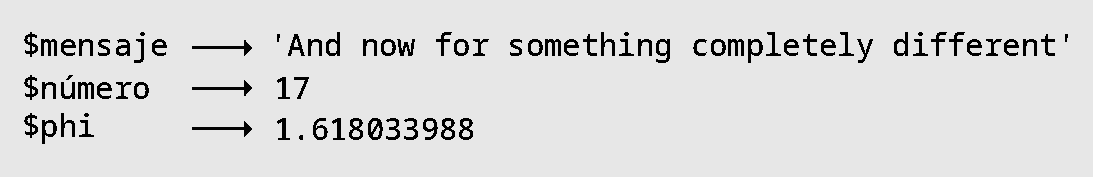
\includegraphics[scale=0.6]{figs/test_5.pdf}}
\caption{Diagrama de estado.}
\label{fig.state2}
\end{figure}



\section{Nombres de las Variables}
\index{variable}

Los programadores generalmente eligen nombres significativos
para sus variables---ellos documentan el uso de la variable.

Los nombres de las variables pueden ser tan largos como tu desees.
Ellos pueden contener letras y números, pero las variables
definidas por el usuario no pueden comenzar con un número. Los nombres de las
variables son sensibles al uso de mayúsculas y minúsculas, 
i.e., {\tt \$mensaje} no es la misma variable que {\tt \$Mensaje} 
o {\tt \$MENSAJE}. Es legal usar letras mayúsculas, pero es convencional
usar solo letras minúsculas para la mayoría de los nombres de las
variables. No obstante, algunas personas prefieren usar {\tt \$TipoTítulo}
para los nombres de sus variables o hasta {\tt \$MAYÚSCULAS} 
para algunas variables especiales.
\index{lower case}
\index{upper case}
\index{title case}
\index{case!lower}
\index{case!upper}
\index{case!title}


\index{Unicode}
\index{ASCII}
A diferencia de muchos otros lenguajes de programación, Perl~6 
no requiere que las letras y dígitos en los nombres de las variables
sean únicamente ASCII. Puedes usar cualquier tipo de letras Unicode, i.e.
letras de cualquier otro lenguaje en el mundo, así que, por ejemplo,
{\tt \$brücke}, {\tt \$payé} or {\tt \$niño} son nombres de variables
válidos, los cuales pueden ser usados por programadores que hablan 
otros idiomas diferentes al inglés (siempre y cuando estos caracteres
Unicode sean correctamente manipulados por tu editor de texto y tu
configuración de pantalla). De la misma manera, en vez de usar 
\verb"$phi" para el nombre de la variable del número aúreo,
podríamos haber usado la \emph{letra griega minúscula phi},
\verb'φ' (Unicode code point U+03C6). Igualmente, podríamos
haber usado la \emph{letra griega minúscula pi}, $\pi$, 
para la muy conocida razoń de la circunferencia del círculo
al diámetro:
\index{golden ratio}
\index{Unicode}
\index{phi}
\index{pi}

\begin{lstlisting}
> my $φ = (5 ** .5 + 1)/2;       # número aúreo
1.61803398874989
> say 'Variable $φ = ', $φ;
Variable $φ = 1.61803398874989
> my $π = 4 * atan 1; 
3.14159265358979
> # podrías también las constante integrada pi o π:
> say pi
3.14159265358979
\end{lstlisting}

El carácter de barra baja, \verb"_", puede aparecer en cualquier
parte del nombre de una variable. Usualmente se usa en nombres con
múltiples palabras, tal como \verb"$tu_nombre" o \verb"$airspeed_of_unladen_swallow". 
\index{underscore character}

Hasta puedes usar guiones para crear lo que se conoce como
``kebab case''\footnote{Porque las variables aparecen estar
atravesadas como las piezas de comida preparadas para un barbacoa.}
y nombrar esas variables \verb"$tu-nombre" or \verb"$airspeed-of-unladen-swallow",
y esto las puede hacer más legibles: un guión \verb'-' es válido en una variable
siempre y cuando sea inmediatamente seguido por un carácter alfanumérico.
Por ejemplo, \verb"$doble-clic" or \verb"$la-niña" son nombres legítimos
de variables. Análogamente, puedes usar un apóstrofo \verb"'" 
(también conocido como comilla simple) entre las letras, así que 
\verb"$isn't" o \verb"$o'brien's-age" son identificadores válidos. 
\index{dash}
\index{apostrophe}
\index{single quote}
\index{quote!single}
\index{kebab case}
\index{case!kebab}


Si les da un nombre ilegal a una variable, consigues 
un error sintáctico:
\index{syntax error}

\begin{lstlisting}
> my $76trombones = 'big parade'
===SORRY!=== Error while compiling <unknown file>
Cannot declare a numeric variable
at <unknown file>:1
------> my $76<HERE>trombones = "big parade";
>
> my $more§ = 100000;
===SORRY!=== Error while compiling <unknown file>
Bogus postfix
at <unknown file>:1
------> my $more<HERE>§ = 100000;
(...)
\end{lstlisting}
%
{\tt \$76trombones} es ilegal porque comienza con un número.
{\tt \$more§} es ilegal porque contiene un carácter ilegal, {\tt
§}. 

Si alguna vez has usado otro lenguaje de programación y 
te has tropezado con un mensaje terso tal como {\tt"SyntaxError: invalid syntax"},
notarás que los diseñadores de Perl han hecho un gran esfuerzo
para proveerte con mensajes de error que sean detallados, útiles
y significativos.
\index{error message}

Muchos lenguajes de programación tienen \emph{palabras claves} o
\emph{palabras reservadas} que son parte de la sintaxis, tales como
{\tt if}, {\tt while}, o {\tt for}, y por lo tanto no pueden ser usadas
para identificar variables porque eso crearía ambigüedad. Dicho problema
no existe en Perl: dado que los nombres de las variables comienzan un sigilo,
el compilador es siempre capaz de diferenciar entre una palabra clave
y una variable. Nombres tales como {\tt \$if} o {\tt \$while} son
sintácticamente identificadores válidos de variables en Perl 
(si estos nombres hacen sentido es un asunto diferente).
\index{sigil}
\index{keyword}
\index{reserved word}


\section{Expresiones y Sentencias}
\label{expr_and_statements}

Una {\bf expresión} es una combinación de términos y operadores.
Los términos pueden ser variables o literales, i.e., valores constantes tales
como un número o una cadena de texto. Al igual que un valor, una variable
es también considerada una expresión. Así que todo lo siguiente
son expresiones legales:
\index{expression}
\index{term}
\index{literal}

\begin{lstlisting}
> 42
42
> my $n = 17;
17
> $n;
17
> $n + 25;
42
>
\end{lstlisting}
%
Cuando escribes una expresión en el prompt, el interpretador
la {\bf evalúa}, lo que significa que encuentra el valor de la expresión.
En esre ejemplo, {\tt \$n} tiene el valor 17 y {\tt \$n + 25} tiene
el valor 42.
\index{evaluate}

Una {\bf sentencia} es unidad de código que tiene un efecto, 
tal como crear una variable or mostrar un valor, y usualmente
necesita terminar con un punto y coma {\tt ;} (aunque el punto y coma
puede algunas veces ser omitido como veremos más adelante):
\index{statement}
\index{semi-colon}

\begin{lstlisting}
> my $n = 17;
17
> say $n;
17
\end{lstlisting}
%

La primera línea es una sentencia de asignación que asigna un 
valor a {\tt \$n}. La segunda línea es una sentencia de impresión 
que muestra el valor de {\tt \$n}.

Cuando escribes una sentencia y después presiona {\tt Enter},
el interpretador la {\bf ejecuta}, lo que significa que hace 
lo que la sentencia dicta.
\index{execute}

Una sentencia puede ser combinada con expresiones usando los operadores
aritméticos. Por ejemplo, podrías escribir:
\index{operator}

\begin{lstlisting}
> my $respuesta = 17 + 25;
42
> say $respuesta;
42
\end{lstlisting}
%

El símbolo \verb'+' es obviamente el operador de adición y,
después de la sentencia de asignación, la variable \verb'$respuesta'
contiene el resultado de la adición. Los términos en cada lado del operador
(aquí 17 y 25) son usualmente llamados los \emph{operadores}
de la operación (una adición en este caso).
\index{operand}
\index{addition operator}
\index{assignment}

Nota que el REPL actualmente muestra el resultado de la asignación
(la primera línea con ``42``), así que la sentencia de impresión 
no era realmente necesaria en este ejemplo \emph{en el REPL};
desde aquí en adelante, para ser breve, generalmente omitiremos las sentencias
de impresión en los ejemplos donde el REPL muestra los resultados.
\index{REPL}

En algunos casos, puedes querer añadir algo a una variable y 
asignar el resultado a la misma variable. Esto se puede escribir
así:

\begin{lstlisting}
> my $respuesta = 17;
17
> $respuesta = $respuesta + 25;
42
\end{lstlisting}
%

Aquí, \verb"$respuesta" es primero declarada con un valor de 17. La siguiente sentencia
asigna a  \verb"$respuesta" el valor actual de  \verb"$respuesta" (i.e., 17) + 25.
Esta operación es tan común en Perl, como en otro lenguajes de programación, que tiene
un atajo:

\begin{lstlisting}
> my $respuesta = 17;
17
> $respuesta += 25;
42
\end{lstlisting}
%

\index{$+=$ augmented assignment operator}
El operador \verb"+=" combina el operador de la adición aritmética 
y el operador de asignación para modificar un valor y aplicar 
el resultado a una variable en un solo paso, así que 
\verb"$n += 2" quiere decir: toma el valor actual de \verb|$n|, agrega
2, y asigna el resultado a \verb|$n|. Esta sintaxis funciona con todos
los operadores aritméticos. Por ejemplo, \verb|-=| realiza una
sustracción y una asignación, \verb|*=| una multiplicación y una asignación, etc.
Además de los operadores aritméticos, también puede ser usado con otros operadores 
tal como el operador de la concatenación de cadena de texto que veremos
más adelante.

Agregar 1 a una variable es una versión muy común de esto, 
y como resultado, existe un atajo, el operador de \emph{incremento},
el cual incrementa su argumento por uno, y devuelve el valor incrementado: 
\index{increment operator}
\index{++ increment operator}
\index{operator!++ (increment)}

\begin{lstlisting}
> my $n = 17;
17
> ++$n;
18
> say $n;
18
\end{lstlisting}
%
Esto se conoce como el operador de incremento prefijo, porque el operador \verb|++|
se coloca antes que la variable a ser incrementada. También hay una versión sufijo (posfijo),
\verb|$n++|, la cual devuelve el valor actual y después incrementa la variable por uno. 
No haría ninguna diferencia en el fragmento de código más arriba, pero el resultado puede
ser diferente en expresiones un poco más complejas.

También hay un operador de decremento \verb|--|, el cual disminuye 
su argumento por uno y existe en la forma prefijo y posfijo. 
\index{decrement operator}
\index{\verb'--' decrement operator}
\index{operator!$--$ (decrement)}



\section{Modo Script}

Hasta ahora hemos ejecutado Perl  en el {\bf modo interactivo}, lo que 
significa que tu interactúas directamente con el interpretador (el REPL).
El modo interactivo es una buena manera de comenzar, si estás trabajando 
con más de varias líneas de código, puede ser un poco torpe y hasta tedioso.
\index{interactive mode}

La alternativa es usar un editor de texto y guardar el código en un archivo de 
texto conocido como un {\bf script} y después ejecutar el interpretador en el 
{\bf modo script} para ejecutar el script. Por convención, los scripts de Perl~6 
tienen nombres que terminan con {\tt .pl}, {\tt .p6} o {\tt .pl6}.
\index{script}
\index{script mode}

Aseguráte de usar un \emph{editor de texto} y no un \emph{programa de procesamiento de texto}
(como MS Word, OpenOffice o LibreOffice Writer). Hay un gran número de editores
de texto disponible gratis. En Linux, podrías usar \emph{vi} (o \emph{vim}), 
\emph{emacs}, \emph{gEdit}, o \emph{nano}. En Windows, puedes usar \emph{notepad} (muy limitado),
o \emph{notepad++}. También hay editores multiplataforma o entorno de desarrollo integrado
(IDES por su siglas en inglés) los cuales proveen la funcionalidad de un editor de texto. 
Entre ellos están \emph{padre}, \emph{eclipse}, o \emph{atom}. Muchos de estos proveen 
varias funcionalidades de resaltado de sintaxis, que puede ayudarte a usar 
la sintaxis correcta (y encontrar algunos errores sintácticos).
\index{syntax!highlighting}
\index{text editor!emacs}
\index{text editor!vi}
\index{text editor!vim}
\index{text editor!gEdit}
\index{text editor!padre}
\index{text editor!eclipse}
\index{text editor!nano}
\index{text editor!notepad++}
\index{text editor!atom}

Una vez que has guardado tu código en un archivo de texto (por ejemplo,
\verb|mi_script.pl6|), puedes ejecutar el programa mediante el siguiente
comando en el prompt del sistema operativo (por ejemplo en una consola de 
Linux or en una ventana \verb|cmd| en Windows):
\begin{lstlisting}
perl6 mi_script.pl6
\end{lstlisting}

Dado que Perl provee ambos modos, 
puedes ejecutar piezas de código en el modo interactivo 
antes que las pongas en un script. Pero existen diferencias entre 
el modo interactivo y el modo script que pueden confundir.
\index{interactive mode}
\index{script mode}

Por ejemplo, si estás usando el interpretador de Perl~6 como una
calculadora, podrías escribir:

\begin{lstlisting}
> my $millas = 26.2;
26.2
> $millas * 1.61;
42.182
\end{lstlisting}

La primera línea asigna un valor a {\tt \$millas} y muestra ese valor.
La segunda línea es una expresión, así que el interpretador la evalúa
y muestra el resultado. Resulta que un maratón es alrededor de 42~kilómetros.

Pero si escribe el mismo código en un script y lo ejecuta, no obtienes
ningún resultado. En el modo script, una expresión por sí misma no tiene
ningún efecto visible. Perl actualmente evalúa la expresión, pero no muestra
el valor a menos que se lo indiques:

\begin{lstlisting}
my $millas = 26.2;
say $millas * 1.61;
\end{lstlisting}

Este comportamiento puede ser confuso al principio. Examinemos
el por qué.

Un script usualmente contiene una secuencia de sentencias. Si hay más 
de una sentencia, los resultados aparecen uno por uno al 
tiempo que las sentencias de impresión se ejecutan.

Por ejemplo, considera el siguiente script:

\begin{lstlisting}
say 1;
my $x = 2;
say $x;
\end{lstlisting}
%
Produce el siguiente resultado:

\begin{lstlisting}
1
2
\end{lstlisting}
%
La sentencia de asignación no produce ningún resultado.

Para comprobar tu entendimiento, escribe las siguientes sentencias
en el interpretador de Perl y observa lo que hacen:

\begin{lstlisting}
5;
my $x = 5;
$x + 1;
\end{lstlisting}

Ahora pon la mismas sentencias en un script y ejecútalo. 
Cuál es el resultado? Transformar cada expresión en una sentencia 
de impresión y después ejecuta el script modificado otra vez.

\section{Modo de una sola línea}

Perl también tiene un \emph{modo de una sola línea} (modo one-liner), el cual te permite 
escribir un script bien corto directamente en el prompt del sistema
operativo. Debido a esto, dicho scripts son conocidos como one-liners.
 En Windows, podría lucir de la siguiente manera:
\index{one-liner mode}
\label{one-liner mode}

\begin{lstlisting}
C:\Users\Laurent>perl6 -e "my $valor = 42; say 'La respuesta es ', $valor;"
La respuesta es 42

\end{lstlisting}

La opción {\tt -e} le dice al compilador que el script
a ser ejecutado no está guardado en un archivo de texto sino
que en cambio está escrito en el prompt entre comillas inglesas
inmediatamente después de dicha opción.

En Unix y Linux, reemplazarías las comillas inglesas con apóstrofos
(o comillas simples)  y los apóstrofos con comillas inglesas:
\index{apostrophe}
\index{quote mark}

\begin{lstlisting}
$  perl6 -e 'my $valor = 42; say "La respuesta es $value";'
La respuesta es 42

\end{lstlisting}

El one-liner más arriba puede no parecer útil, pero 
one-liners desechables pueden ser muy prácticos para realizar
operaciones simples, tal como modificar un archivo que no
está formateado apropiadamente, sin tener que guardar un script
en archivo separado antes de ejecutarlo.  

No daremos ningunos detalles adicionales sobre el modo 
de una sola línea, pero daremos más ejemplos útiles más
adelante en este libro; por ejemplo,
Subsección~\ref{one-liner-example},
Subsección~\ref{rot13_oneliner} (resolviendo el ejercicio ``rot-13''), o
Subsección~\ref{sol_cartalk} (resolviendo el ejercicio sobre 
letras dobles consecutivas). 



\section{Orden de Operaciones}
\index{order of operations}
\index{PEMDAS}
\index{operator precedence}
\index{precedence!operator}

Cuando una expresión contiene más de un operador, el orden 
de evaluación depende en el {\bf orden de operaciones} o 
la \emph{precedencia de operadores}. Para los operadores matemáticos,
Perl sigue la convención matemática. El acrónimo {\bf PEMDAS}\footnote{Los estudiantes 
estadounidenses se les enseña a usar el mnemónico 
"Please Excuse My Dear Aunt Sally" para recordar el orden 
correcto de las letras en el acrónimo.} es una manera muy útil de recordar
las reglas\footnote{En español, podrías utilizar "Por Favor Excusa Mi Dragón Azul Sancho" para
recordar el orden correcto.}:
 
\begin{itemize}

\item {\bf P}aréntesis tienen la mayor precedencia y pueden ser 
usado para forzar una expresión a evaluar en el orden que deseas.
Dado que las expresiones en paréntesis son evaluadas primero, 
{\tt 2 * (3-1)} es 4, y {\tt (1+1)**(5-2)} es 8.  También puedes usar 
paréntesis para hacer una expresión más legible, como en {\tt (\$minuto * 100) / 60},
aunque no cambia el resultado.
\index{$()$ parenthesis operator}

\item {\bf E}xponente (potenciación) es la siguiente en el nivel de precedencia, así
que {\tt 1 + 2**3} es 9 (1 + 8), no 27, y {\tt 2 * 3**2} es 18, no 36.
\index{$**$ exponentiation operator}
\index{operator!$**$ (exponentiation)}

\item {\bf M}ultiplicación y {\bf D}ivisión tiene mayor precedencia
  que {\bf A}dición y {\bf S}ustracción.  Por lo tanto, {\tt 2*3-1} es 5, no
  4, y {\tt 6+4/2} es 8, no 5.
\index{$*$ multiplication operator}
\index{operator!$*$ (multiplication)}
\index{$/$ division operator}
\index{operator!$/$ (division)}

\item Operadores con la misma precedencia son usualmente evaluados
de izquierda a derecha (excepto la potenciación). Así que en la expresión
{\tt \$grados / 2 * pi}, la división ocurre primero y el resultado 
es multiplicado por {\tt pi}, el cual no es el resultado esperado. (Nota que 
{\tt pi} no es una variable, pero una constante predefinida en Perl~6, y por lo tanto
no requiere un sigilo.) Para dividir por $2 \pi$, puedes usar paréntesis: 
\index{sigil}
\index{pi}
  
\begin{lstlisting}
my $result = $degrees / (2 * pi);  
\end{lstlisting}  
 
o escribir 
  {\tt \$grados / 2 / pi} o {\tt \$grados / 2 / $\pi$}, lo cual
  divide \verb'$grados' por 2, y después divide el resultado de esa
  operación por $\pi$ (el cual es equivalente a \verb'$grados'
  dividido por $2 \pi$).

\end{itemize}

Yo trato de no recordar la precedencia de los operadores. Si no puedo 
determinar la precedencia al mirar la expresión, uso paréntesis para
hacerlo obvio. Si no sé cuál de dos operadores tiene la mayor precedencia, entonces 
la siguiente persona manteniendo mi código podría tampoco saberlo.
\index{precedence}
\index{parentheses}


\section{Operaciones de Cadena de Texto}
\label{string_operations}
\index{string!operation}
\index{operator!string}
\index{coercion}
\index{type!coercion}

En general, no puedes realizar operaciones matemáticas con cadenas de texto,
a menos que las cadenas de texto se parezcan tanto a los números que 
Perl las transforma o \emph{coacciona} en números y todavía hace sentido.
Así que los siguientes casos son ilegales:

\begin{lstlisting}
'2'-'1a'    'eggs'/'easy'    'third'*'a charm'
\end{lstlisting}
%

Por ejemplo, esto produce un error:

\begin{lstlisting}
> '2'-'1a'
Cannot convert string to number: trailing characters after number 
in '1?a' (indicated by ?)
  in block <unit> at <unknown file>:1
\end{lstlisting}
%

Pero la siguiente expresiones son válidas porque estas cadenas de texto
pueden ser coaccionadas en números sin ninguna ambigüedad:
\begin{lstlisting}
> '2'-'1'
1
> '3'/'4'
0.75
\end{lstlisting}
%

El operador \verb'~' realiza la {\bf concatenación de cadenas de texto}, 
lo cual quiere decir que une las cadenas de texto al enlazarlas de
extremo a extremo. Por ejemplo:
\index{string concatenation}
\index{string!concatenation}

\begin{lstlisting}
> my $primera = 'hidro'
throat
> my $segunda = 'avión'
warbler
> $primera ~ $segunda
hidroavión
\end{lstlisting}
%
El operador {\tt x} también funciona con cadenas de texto; básicamente
realiza repeticiones. Por ejemplo:
\index{string repetition}

\begin{lstlisting}
> 'ab' x 3;
ababab
> 42 x 3
424242
> 3 x 42
333333333333333333333333333333333333333333
\end{lstlisting}

Nota que, aunque el operador {\tt x} se parece al operador
de multiplicación que escribimos a mano, {\tt x} obviamente 
no es conmutativo, contrario al operador de multiplicación 
{\tt *}. El primer operando es una cadena de texto o es coaccionado
en una (i.e., transformado en una cadena de texto:
{\tt 42} es coaccionado en {\tt '42'})  , y el segundo operando
tiene que ser un número o algo que pueda ser transformado en 
un número.
\index{commutativity}
\index{coercion}


\section{Comentarios}
\index{comment}

A medida que los programas crecen y se vuelven más complicados,
ellos se vuelven menos legible. Los lenguajes formales son denso, y es usualmente
difícil mirar a un fragmento de código y descifrar lo que está haciendo,
o por qué lo está haciendo.

Por esta razón, es muy buena idea agregar notas a tus programas que expliquen en un
lenguaje natural lo que el programa hace. Estas notas son conocidas como {\bf comentarios},
y comienzan con el símbolo \verb|#|:

\begin{lstlisting}
# computar el porcentaje de la hora que ha pasado
my $porcentaje = ($minuto * 100) / 60;
\end{lstlisting}
%
En este caso, el comentario aparece en una línea por sí mismo. También puedes
colocar comentarios al final de una línea:

\begin{lstlisting}
$porcentaje = ($minuto * 100) / 60;     # porcentaje de una hora
\end{lstlisting}
%
Todo desde el inicio de {\tt \#} al final de la línea es ignorado---lo que significa
que no tiene un efecto en el ejecución del programa.

Los comentarios son más útiles cuando documentan características del código
que no obvias. Es razonable asumir que el lector puede descifrar lo que 
hace el código; es más útil explicar explicar el {\em por qué}.

Este comentario es redundante con el código e inservible:

\begin{lstlisting}
my $valor = 5;        # asignar 5 a $valor
\end{lstlisting}
%
Por el contrario, este comentario contiene información útil que no está
presente en el código:

\begin{lstlisting}
my $velocidad = 5;     # la velocidad es en metros/segundos. 
\end{lstlisting}
%
Nombres de variables que son buenos y adecuados pueden reducir la necesidad 
de comentario, pero nombres muy largos pueden hacer expresiones sean difíciles
de leer, por lo tanto debe existir un balance.
\index{variable name}


\section{Depuración de Programas}
\index{debugging}
\index{bug}

Tres tipos de errores pueden ocurrir en un programa: errores
sintácticos, errores al tiempo de ejecución, y  errores semánticos.
Es muy útil saber distinguirlos para ratrearlos más rápido.

\begin{description}

\item[Error sintáctico] La ``sintaxis'' se refiere a la estructura de un 
programa. Por ejemplo, los paréntesis deben estar en parejas, así que 
{\tt (1 + 2)} es legal mientras {\tt 8)} es un \emph{error sintáctico}.
\footnote{Aquí estamos usando ``error sintáctico'' como un cuasi-sinónimo
para ``error al tiempo de compilación``; ellos no son exactamente la misma cosa
(en teoría, puedes tener errores sintácticos que no son errores al tiempo
de compilación y viceversa), pero se pueden considerar aquí lo mismo por razones
prácticas. En Perl~6, errores al tiempo de compilación tienen la cuerda de texto
``===SORRY!==='' al inicio del mensaje de error.}

\index{error!syntax}
\index{error message}
\index{syntax} 
\index{syntax!error}

Si en tu programa hay un error sintáctico, Perl muestra 
un mensaje de error y abandona la ejecución sin siquiera 
comenzar a ejecutar el programa. Durante las primeras semanas de 
tu carrera de programación, podrías invertir mucho tiempo rastreando
errores sintácticos. A medida que ganas experiencia, cometerás menos errores
y lo encontraras más rápido.


\item[Error al tiempo de ejecución] El segundo tipo de error es un 
error al tiempo de ejecución, llamado así porque el error no aparece hasta que 
el programa ha comenzado a ejecutarse. Estos errores también son conocidos
como \emph{excepciones} porque ellos usualmente indican que algo excepcional (y malo)
ha ocurrido. 
\index{runtime error}
\index{error!runtime}
\index{exception} 
\index{safe language} 
\index{language!safe}

Los errores al tiempo de ejecución son raros en programas simples 
que verás en los primeros capítulos, así que podría pasar un rato antes
que encuentres uno. Ya hemos visto un ejemplo de tales errores, aunque, 
al inicio de la Sección~\ref{string_operations} (p.~\pageref{string_operations}), 
cuando intentamos sustraer \verb"'2'-'1a'".


\item[Error semántico] El tercer tipo de error es \emph{semántico}, lo que
significa que está relacionado con el significado. Si en tu programa hay un error
semántico, el programa se ejecutará sin generar mensajes de error. Específicamente,
hará lo que \emph{dijiste} que hiciera, pero no lo que habías \emph{previsto}.
\index{semantic error}
\index{error!semantic}
\index{error message}

La identificación de errores semánticos pueden ser complicada porque requiere
que trabajes de atrás hacia adelante mediante la observación de la salida
del programa y tratando de descifrar lo que el programa esta haciendo.

\end{description}


\section{Glosario}

\begin{description}

\item[Variable]  Informalmente, un nombre que hace referencia a un valor. En términos
precisos, una variable es un contenedor que tiene un nombre y almacena un valor.
\index{variable}

\item[Asignación]  Un sentencia que asigna un valor a una variable.
\index{assignment}

\item[Diagrama de estado]  Una representación gráfica de un conjunto de variables
y los valores a los que hacen referencia.
\index{state diagram}

\item[Palabra clave]  Una palabra reservada que es usada para parsear
un programa; en muchos lenguajes, no puedes usar palabras claves tales como
{\tt if}, {\tt  for}, y {\tt while} como nombres de variables.
Este problema usualmente no ocurre en Perl porque los nombres de variables
comienzan con un \emph{sigilo}.
\index{keyword}
\index{sigil}

\item[Operando] Un valor o término al lado de un operador que es usado
en su evaluación.
\index{operand}

\item[Término]  Una variable or valor literal.
\index{term}

\item[Expresión]  Una combinación de operadores y términos que 
representan un valor único.
\index{expression}

\item[Evaluar]  Simplificar una expresión al realizar las operaciones 
para obtener un valor único.
\index{evaluate}

\item[Sentencia]  Una sección de código que representa un comando o una acción. Hasta ahora,
las sentencias que hemos visto son las asignaciones y las sentencias de impresión. Las sentencias
usualmente terminan con un punto y coma.
\index{statement}

\item[Ejecutar]  Poner una sentencia en acción y hacer lo que dice.
\index{execute}

\item[Modo interactivo (o modo interpretador):] Una manera de usar el interpretador 
de Perl al escribir código en el prompt.
\index{interactive mode}

\item[Modo script] Una manera de usar el interpretador 
de Perl para leer código desde un script y ejecutarlo.
\index{script mode}

\item[Modo de una sola línea (one-liner)] Una manera de usar el interpretador 
de Perl para leer código pasado al prompt del sistema operativo 
y ejecutarlo.
\index{one-liner mode}

\item[Script] Un programa almacenado en un archivo de texto.
\index{script}

\item[Order de operaciones]  Reglas que dictan el orden en el que las expresiones
que contienen varios operadores y operandos son evaluadas.
También se conoce como precedencia de operadores.
\index{order of operations}
\index{operator precedence}
\index{precedence!operator}

\item[Concatenar]  Unir dos cadenas de texto de extremo a extremo.
\index{concatenation}

\item[Comentario]  Información en una programa que está dirigida a otros programadores
(o cualquier persona leyendo el código fuente) y que no tiene ningún efecto en 
la ejecución del programa.
\index{comment}

\item[Error sintáctico]  Un error en un programa que lo hace imposible
parsear (y por lo tanto imposible de compilar y ejecutar).
\index{syntax!error}

\item[Excepción]  Un error que es detectado mientra que el programa se ejecuta.
\index{exception}

\item[Semántica]  El significado de un programa.
\index{semantics}

\item[Error semántico] Un error en un programa que causa que haga algo 
diferente a lo que programador pretendía hacer.
\index{semantic error}

\end{description}


\section{Ejercicios}

\begin{exercise}

Repetimos nuestro consejo mencionado en el capítulo anterior,
cuando aprendas algo nuevo, deberías probarlo en el modo interactivo
(de REPL) y cometer errores a propósito para ver que es lo que no funciona.
\index{interactive mode}
\index{REPL}

\begin{itemize}

\item Hemos visto que {\tt \$n = 42} es legal. ?`Y {\tt 42 = \$n}?

\item ?`Qué acerca de {\tt \$x = \$y = 1}? (Pista: nota que 
tendrás que declarar ambas variables, por ejemplo con una sentencia
tal como {\tt my \$x; my \$y;} o posiblemente {\tt my (\$x, \$y);},
antes de que ejecutes lo anterior.)

\item En algunos lenguajes, las sentencias no tienen que terminar con un
punto y coma, {\tt ;}. ?`Qué pasa en el modo script si omites un punto y
coma al final de una sentencia de Perl?
\index{semi-colon}

\item ?`Qué pasa si pones un punto al final de una sentencia?

\item En notación matemática puedes multiplicar $m$ y $n$ así: $m n$.
?`Qué pasa si tratas de hacerlo en Perl?

\end{itemize}

\end{exercise}


\begin{exercise}

Practica usando el interpretador de Perl como una calculadora:
\index{calculator}

\begin{enumerate}

\item El volumen de una esfera con radio $r$ es $\frac{4}{3} \pi r^3$.
?`Cuál es el volumen de una esfera con radio 5?

\item Supón que el precio inicial de un libro es \$24.95,
pero la librería obtiene un 40\% de descuento. El envío
cuesta \$3 por la primera copia y 75 centavos por cada copia adicional.
?`Cuál es el precio total de 60 copias?

\item Si dejo la casa a la 6:52 a.m. y corro 1 milla a paso suave
(8 min. 15 seg. por milla), después 3 millas a paso rápido 
(7 min. 12 seg por milla) y 1 milla a paso suave otra vez.
?`Qué hora es cuando termino con mi ejercicio?
\index{running pace}

\end{enumerate}
\end{exercise}



\chapter{Funciones}
\label{funcchap}

En el contexto de la programación, una {\bf función}
es usualmente una secuencia de sentencias con nombre
que realizan una computación. En Perl, las funciones
son usualmente llamadas {\bf subrutinas} y los dos términos
(por ahora) pueden considerarse  más o menos equivalente. Cuando defines
una función, especificas el nombre y la secuencia de sentencias.
Después, cuando quieras realizar la computación, puedes 
``invocar`` la función por el nombre y esto ejecutará la secuencia
de sentencias dentro de la definición de la función.
\index{function}

Perl viene como muchas funciones integradas que son muy útiles.
Ya has visto algunas de ellas: por ejemplo, {\tt say} es una función 
integrada, y veremos más en el curso de este libro. Y si Perl no tiene
una función que hace lo que deseas hacer, tú puedes construirla. Esto
te enseña lo básico de las funciones y cómo construir una.

\section{Llamadas de Funciones}
\label{functionchap}
\index{function!call}

Ya hemos visto algunos ejemplos de {\bf llamadas de funciones}:

\begin{lstlisting}
> say 42;
42
\end{lstlisting}
%
El nombre de la función es {\tt say}. La expresión que sigue el
nombre de la función se llama el {\bf argumento} de la función.
La función {\tt say} causa que el argumento se ha mostrado en 
la pantalla. Si necesitas pasar varios argumentos a la función, 
solo separa los argumentos con comas:

\begin{lstlisting}
> say "La respuesta a la pregunta absoluta es ", 42;
La respuesta a la pregunta absoluta es 42
\end{lstlisting}
%

Muchos lenguajes de programación requieren que los argumentos de
la función se encuentren dentro de paréntesis. Esto no es requerido
(y usualmente no recomendado) en Perl~6 para la mayoría de 
las funciones integradas (excepto cuando se necesita para 
precedencia), pero si usas paréntesis, deberías evitar insertar 
espacios entre el nombre de la función y el paréntesis izquierdo,
Por ejemplo, la función {\tt round} usualmente toma dos argumentos:
el valor a ser redondeado y la unidad o escala.
Puedes invocarla en cualquiera de las siguientes formas:

\begin{lstlisting}
> round 42.45, 1;
42
> round 42.45, .1;
42.5
> round(42.45, .1);      # Pero no: round (42.45, .1);
42.5
> round( 42.45, .1);     # Espacio *después* del paréntesis izq. es OK 
42.5
\end{lstlisting}
\index{parentheses!argument in}

Los programadores de Perl con experiencia prefieren omitir los 
paréntesis cuando ellos pueden. Esto hace posible encadenar varias 
funciones con una sintaxis más limpia. Considera por ejemplo
la diferencia entre estas dos llamadas:

\begin{lstlisting}
> say round 42.45, 1;
42
> say(round(42.45, 1));
42
\end{lstlisting}

La segunda sentencia dice explícitamente lo que está pasando,
pero la acumulación de paréntesis actualmente no hace las cosas
muy claras. Por el contrario, la primera sentencia puede ser
considerada como una línea de tuberías que se puede leer de derecha 
a izquierda: la última función a la derecha, {\tt round}, toma dos
argumentos, {\tt 42.45, 1}, y el valor producido por {\tt round}
es pasado como un argumento a {\tt say}.

Es muy común decir que una función ``toma`` uno o varios
argumentos y ``devuelve`` un resultado. El resultado es también
llamado el {\bf valor de retorno}.
\index{argument}
\index{return!value}

Perl provee varias funciones que convierten valores de un
tipo a otro. Cuando se invocan con un solo argumento,
la función {\tt round} toma cualquier valor y lo convierte
en un número entero, o por el contrario se queja:
\index{conversion!type}
\index{type!conversion}
\index{round function}
\index{function!round}

\begin{lstlisting}
> round 42.3;
42
> round "yes"
Cannot convert string to number: base-10 number must begin with valid 
digits or '.' in '<HERE>yes' (indicated by <HERE>)
  in block <unit> at <unknown file> line 1
\end{lstlisting}

%
Nota que, en Perl~6, muchas funciones integradas pueden también
usar la sintaxis de la \emph{llamada de método} con la así 
llamada notación de punto. Las siguientes sentencias muestran el 
mismo resultado:
\index{invocation!method}
\index{method invocation}
\begin{lstlisting}
> round 42.7;    # Sintaxis de la llamada de función
43
> 42.7.round;    # Sintaxis de la llamada de método
43
\end{lstlisting}
%
La función {\tt round} puede redondear valores racionales
y valores coma flotante. Hay un método {\tt Int} que también
convierte valores numéricos no enteros en enteros, pero
no redondea; corta la parte fraccional:
\index{Int method}
\index{method!Int}

\begin{lstlisting}
> round 42.7
43
> 42.7.Int
42
\end{lstlisting}

Volveremos a los métodos en la siguiente sección.

La función integrada {\tt Rat} convierte números
enteros y cadenas de texto en números racionales (si es posible):
\index{Rat function}
\index{function!Rat}

\begin{lstlisting}
> say 4.Rat;
4
> say 4.Rat.WHAT;
(Rat)
> say Rat(4).WHAT;
(Rat)
> say Rat(4).nude;
(4 1)
> say Rat('3.14159');
3.14159
> say Rat('3.14159').nude
(314159 100000)
\end{lstlisting}
%
(Como podrás recordar de la Sección~\ref{values_and_types}, 
el método \verb'nude' muestra el \emph{nu}merador y  
\emph{de}nominador de un número racional.)

Finalmente, {\tt Str} convierte su argumento a una cadena de texto:
\index{Str function}
\index{function!Str}

\begin{lstlisting}
> say 42.Str.WHAT
(Str)
> say Str(42).WHAT;
(Str)
\end{lstlisting}

\index{coercion}
\index{type!coercion}
Nota que estas funciones de conversión de tipo no necesitan ser
invocadas explícitamente, dado que Perl intentará hacer lo correcto
en muchos de los casos. Por ejemplo, si tienes una cadena de texto
que se parece a un número entero, Perl \emph{coaccionará} la cadena 
de texto en un entero para ti si tratas de aplicarle una operación 
aritmética:

\begin{lstlisting}
> say "21" * "2";
42
\end{lstlisting}

Igualmente, los enteros serán coaccionados en cadenas de texto
si aplicas el operador de la concatenación de cadena de texto
sobre ellos:

\begin{lstlisting}
> say 4 ~ 2;
42
> say (4 ~ 2).WHAT;
(Str)
\end{lstlisting}

La coacción puede hasta pasar dos veces dentro de la misma expresión
si necesario:

\begin{lstlisting}
> say (4 ~ 1) + 1;
42
> say ((4 ~ 1) + 1).WHAT;
(Int)
\end{lstlisting}

\section{Funciones y Métodos}
\index{function}
\index{method}

Un método es similar a una función---toma argumentos y 
devuelve un valor---pero la sintaxis de llamada es
diferente. Con una función, especificas el nombre de la función
seguido de sus argumentos. Un método, por el contrario, usa 
la notación de punto: tu especificas el nombre del objecto
sobre el cual el método es invocado, seguido por un punto y
el nombre del método (y posiblemente argumentos adicionales).

% 
Una llamada de método es usualmente conocida como una 
{\bf invocación} \index{invocation}. Las diferencias más
profundas entre funciones y métodos se volverá aparente 
más adelante, cuando estudiemos la programación orientada
a objetos (en el Capítulo~\ref{objects}).
\index{invocation!method}
\index{method invocation}

Por el tiempo presente, podemos consider que la diferencia
es esencialmente un asunto de una sintaxis diferente de 
llamada cuando se usan las funciones integradas de Perl. La mayoría
de las funciones integradas en Perl aceptan la sintaxis de la llamada
de función y la sintaxis de la invocación de método. Por ejemplo,
las siguientes sentencias son equivalentes:

\begin{lstlisting}
> say 42;              # sintaxis de la llamada de función
42
> 42.say;              # sintaxis de la invocación de método
42
\end{lstlisting}
%

También puedes encadenar subrutinas con ambas formas
sintácticas:

\begin{lstlisting}
> 42.WHAT.say;         # sintaxis de método
(Int)
> say WHAT 42;         # sintaxis de función
(Int)
> say 42.WHAT;         # sintaxis mixta
(Int)
\end{lstlisting}
%

Depende de ti cuál de las formas prefieres usar, pero
usaremos ambas formas, aún solo sea para acostumbrarnos
a ambas.

\section{Funciones Matemáticas}
\index{math function}
\index{function!math}

Perl provee muchas de las funciones matemáticas familiares.

Para algunas funcionesno tan comunes, podría necesitar un
módulo especializado tal com \verb'Math::Matrix' o
\verb'Math::Trig'. Un {\bf módulo} es un archivo de texto 
que contiene una colección de funciones que están relacionadas.
\index{module}

Antes de que usemos las funciones en un módulo, tenemos que importarlo
la sentencia {\bf use}:

\begin{lstlisting}
use Math::Trig;
\end{lstlisting}
%
Esta sentencia importará un número de funciones que serás capaz de usar
como si tu las hubieses definido en el archivo de código principal,
por ejemplo \verb|grad2rad| convierte un valor angular desde grados
a radianes o \verb|rad2grad| que hace la conversión opuesta.

Para la mayoría de funciones matemáticas comunes, sin embargo, no necesitas
tener ningún módulo \verb|matemático|, dado que dichas funciones
ya están incluidas en núcleo del lenguaje:

\begin{lstlisting}
> my $nivel-ruido = 5.5;
5.5
> my $nivel-señal = 125.6;
125.6
> my $decibelios = 10 * log10 $nivel-señal / $nivel-ruido;
13.5862694990693
\end{lstlisting}
%
\index{log10 function}
\index{function!log10}
El primer ejemplo usa \verb"log10" (logaritmo común)
para computar la razón de señal y ruido en decibelios
(asumiendo que \verb|nivel-señal| y \verb|nivel-ruido| sean 
definidos en las propias unidades). Perl también provee una 
función {\tt log}, la cual, cuando recibe un argumento,
computa el logaritmo en base {\tt e} del argumento y,
cuando recibe dos argumentos, computa el logaritmo del primer
argumento en base del segundo argumento:

\begin{lstlisting}
> say e;                 # e es predefinada como la constante de Euler
2.71828182845905
> my $val = e ** e;
15.1542622414793
> say log $val;          # logaritmo natural
2.71828182845905
> say log $val, e;       # logaritmo en base e o logaritmo natural
2.71828182845905
> say log 1024, 2;       # logaritmo binario o logaritmo en base 2
10
\end{lstlisting}
%
\index{log function}
\index{function!log}

Perl también provee muchas de las funciones trigonométricas
comunes:

\begin{lstlisting}
> my $radianes = 0.7;
0.7
> my $altura = sin $radianes;
0.644217687237691
\end{lstlisting}

\index{sin function}
\index{radian}
\index{trigonometric function}
\index{function!trigonometric}
Este ejemplo encuentra el seno de \verb|$radianes|. El 
nombre de la variable es una pista a que el {\tt sin} y 
otras funciones trigonométricas ({\tt cos}, {\tt tan}, etc.) toman
argumentos en radianes. Para convertir de grados a radianes, puedes
usar la función \verb'deg2rad' del  módulo \verb|Math::Trig|, o
simplemente divide por 180 y multiplica por $\pi$:

\begin{lstlisting}
> my $grados = 45;
45
> my $radianes = $grados / 180.0 * pi;    # pi, constante predefinida 
0.785398163397448
> say sin $radianes;       # debería ser la raíz cuadrada de 2 divida por 2
0.707106781186547
\end{lstlisting}
%
La expresión {\tt pi} es una constante predefinida de una
aproximación de $\pi$, precisa alrededor de 14 dígitos:
\index{pi}

Si sabes trigonometría, puedes verificar el resultado anterior
al compararlo con la raíz cuadrada de 2 dividida por 2:
\index{sqrt function}
\index{function!sqrt}

\begin{lstlisting}
> say sqrt(2) / 2;
0.707106781186548
\end{lstlisting}
%

\section{Composición}
\index{composition}

Hasta ahora, hemos discutidos los elementos de un programa---variables,
expresiones, y sentencias---aisladamente, sin discutir sobre
cómo combinarlos.

Una de las características más útiles de los lenguajes de programación
es su habilidad de tomar pequeños componentes y {\bf componer} estos
componentes, i.e.,
combinarlos de tal manera que el resultado de uno es la entrada
de otro. Por ejemplo, el argumento de una función  puede ser cualquier
tipo de expresión, incluyendo operadores aritméticos:

\begin{lstlisting}
> my $grados = 45;
45
> my $altura = sin($grados / 360.0 * 2 * pi);
0.707106781186547
\end{lstlisting}
%
Aquí, hemos usados paréntesis para el argumento de la función
{\tt sin} para clarificar que todas las operaciones aritméticas
sean completadas antes que la función {\tt sin} sea actualmente
llamada, para que así use el resultado de estas operaciones 
como su argumento.

Puedes componer llamadas de funciones:

\begin{lstlisting}
> my $x = 10;
10
>  $x = exp log($x+1)
11
\end{lstlisting}
%
Casi en cualquier lado que puedes poner un valor, puedes poner
una expresión arbitraria, con una excepción: el lado izquierdo 
de la sentencia de asignación tiene que ser el nombre de una
variable, posiblemente con su declaración. Casi cualquier otra expresión
en el lado izquierdo es un error sintáctico \footnote{Veremos esta rara
excepción a esta regla más tarde}:


\begin{lstlisting}
> my $horas = 1;
1
> my $minutos = 0;
0
> $minutos = $horas * 60;        # correcto 
60
> $horas * 60 = $minutos;        # incorrecto!!
Cannot modify an immutable Int
  in block <unit> at <unknown file> line 1
\end{lstlisting}
%
\index{syntax error}


\section{Agregar Nuevas Funciones (o Subrutinas)}

\index{subroutine}
Hasta ahora, hemos solo usado las funciones que vienen con Perl,
pero también es posible agregar nuevas funciones. En Perl, las 
funciones definidas por el usuario son usualmente conocidas 
como subrutinas, pero podrías eligir cualquiera de las dos
palabras. 

Una {\bf definición de función} comienza con la palabra clave 
{\tt sub} (abreviación de subrutina) y especifica el nombre de una
nueva subrutina y la secuencia de sentencias que serán ejecutadas
cuando función es llamada.
\index{function}
\index{function!definition}
\index{definition!function}
\index{sub}

Este es un ejemplo de una subrutina que cita el famoso discurso
"I Have a Dream" de Martin Luther King en el Lincoln Memorial en
Washington (1963):

\begin{lstlisting}
sub imprimir-discurso() {
    say "Let freedom ring from the prodigious hilltops of New Hampshire.";
    say "Let freedom ring from the mighty mountains of New York.";
}
\end{lstlisting}
%
{\tt sub} es la palabra clave que indica que esto es una definición 
de subrutina. El nombre de la función es \verb|imprimir-discurso|.
Las reglas para los nombres de subrutinas son las mismas reglas 
para los nombres de variables: letras, números, y guiones bajos son
legales, al igual que un guión o un apóstrofo entre letras, pero
el primer carácter debe ser una letra o un guion bajo. No deberías
usar una palabra clave usada por el lenguaje (tales como {\tt if} 
o {\tt while}) como el nombre de una función (en algunos casos, podría
actualmente funcionar pero sería algo confuso, por lo menos 
para el lector humano).
\index{sub!keyword}
\index{keyword!sub}
\index{argument}

Los paréntesis vacíos después del nombre indican que esta función 
no toma ningún argumento. En tal caso los argumentos son opcionales,
pero son requeridos cuando los parámetros necesitan ser definidos para
la subrutina.
\index{parentheses!empty}
\index{header}
\index{body}

\index{indentation}
La primera línea de la definición de una subrutina es algunos
veces llamada la {\bf cabecera}; el resto es conocido como el
{\bf cuerpo} de la subrutina. El cuerpo tiene que ser un bloque de
código colocado entre llaves y puede contener una cantidad
indefinida de sentencias. Aunque no existe una regla que lo requiera,
es buena práctica (y muy recomendada) la indentación de las sentencias
en el cuerpo con varios espacios delanteros, debido a que facilita
descifrar visualmente donde el cuerpo de la función inicia y termina.
\index{curly bracket}
\index{curly brace}
\index{bracket!curly}

Ten presente que no puedes utilizar la sintaxis de invocación de método
con las subrutinas (tal como \verb|imprimir-discurso|) que escribas: 
debes llamarlas con la sintaxis de llamada de función.
\index{method!invocation}
\index{function!call}
\index{invocation!method}
\index{method invocation}

Las cadenas de texto en las sentencias de impresión están rodeadas
por comillas inglesas. En este caso específico, las comillas simples
se podrían haber usado para obtener el mismo resultado, pero
hay otros casos donde los dos tipos de comillas no harían lo mismo,
así que tendrás que elegir una de las dos dependiendo de las 
circunstancias.
\index{double quote}
\index{quote!double}
\index{single quote}
\index{quote!single}

Muchas personas usan las comillas inglesas en los casos
donde una comilla simple (la cual también es un apóstrofo)
aparece en una cadena de texto:
\index{apostrophe}
\begin{lstlisting}
say "And so we've come here today to dramatize a shameful condition.";
\end{lstlisting}
%
De igual manera, podrías utilizar comillas simples 
cuando las comillas inglesas aparecen en una cadena de texto:
\begin{lstlisting}
say 'America has given the Negro people a bad check, 
     a check which has come back marked "insufficient funds."';
\end{lstlisting}
%
Sin embargo, existe una diferencia más importante entre las 
comillas simples y las comillas inglesas: las comillas inglesas
permiten la interpolación de variables, lo cual no es posible
con el uso de comillas simples. La interpolación de variables
se refiere a que si el nombre de una variable aparece dentro
de una cadena de texto rodeada por comillas inglesas, dicho 
nombre será reemplazado por el valor de la variable; dentro una 
cadena de texto rodeada por comillas simples, el nombre de la 
variable aparecerá literalmente.
Por ejemplo:
%
\begin{lstlisting}
my $var = 12;
say "La edad del niño es $var.";         # -> La edad del niño es 12.
say 'La edad de la niña es $var.';       # -> La edad de la niña es $var.
\end{lstlisting}
\index{interpolation}
\index{variable!interpolation}
%
La edad de la niña no se muestra porque se quiera mantener un
secreto. En la primera cadena de texto, \verb|$var| es 
simplemente reemplazada dentro de la cadena por su valor, 12, porque
la cadena de texto está rodeada con comillas inglesas; en la segunda
cadena de texto, \verb|$var| no es reemplazada por su valor porque las 
comillas simples están supuestas a proveer un citado más literal. 
Existen otros tipos de citados que ofrecen un mayor control sobre la
manera en que las variables y los caracteres especiales son mostrados 
en la salida, pero las comillas simples y las comillas inglesas
son las más útiles.

La sintaxis para llamar una nueva subrutina es la misma usada
para llamar las funciones integradas:

\begin{lstlisting}
> imprimir-discurso();
Let freedom ring from the prodigious hilltops of New Hampshire.
Let freedom ring from the mighty mountains of New York.
\end{lstlisting}
%

No obstante, no puedes utilizar la sintaxis de invocación de método
con tales subrutinas. Más tarde veremos en este libro (ve
Capítulo~\ref{objects}) cómo crear métodos. Por el tiempo presente,
permaneceremos con la sintaxis de llamada de función.
\index{invocation!method}
\index{method invocation}

Una vez que has definido una subrutina, puedes usarla dentro
de otra subrutina. Por ejemplo, para repetir el fragmento anterior
del discurso de King, podríamos escribir una subrutina llamada 
\verb|repetir-discurso|:

\begin{lstlisting}
sub repetir-discurso() {
    imprimir-discurso();
    imprimir-discurso();
}
\end{lstlisting}
%
Y después llamar \verb|repetir-discurso|:

\begin{lstlisting}
> repetir-discurso();
Let freedom ring from the prodigious hilltops of New Hampshire.
Let freedom ring from the mighty mountains of New York.
Let freedom ring from the prodigious hilltops of New Hampshire.
Let freedom ring from the mighty mountains of New York.
\end{lstlisting}
%
No obstante, no es así como prosigue el discurso.


\section{Definiciones y Usos}
\index{function!definition}

Juntando los fragmentos de código de la sección anterior, el
programa entero luce así:

\begin{lstlisting}
sub imprimir-discurso () {
    say "let freedom ring from the prodigious hilltops of New Hampshire.";
    say "Let freedom ring from the mighty mountains of New York.";
}
sub repetir-discurso () {
    imprimir-discurso();
    imprimir-discurso();
}
repetir-discurso();
\end{lstlisting}
%
Este programa contiene dos definiciones de subrutinas: \verb|imprimir-discurso|
y \verb|repetir-discurso|. Las definiciones de funciones pueden ser ejecutadas
como otras sentencias, pero el efecto es crear la función. Las sentencias
dentro de la función no son ejecutadas hasta que la función es llamada, y
la definición de la función no genera ninguna salida.

No necesitas crear una subrutina antes de ejecutarla,
la definición de la función puede venir después de la llamada:

\begin{lstlisting}
repetir-discurso;
sub repetir-discurso() {
    imprimir-discurso;
    imprimir-discurso;
}
sub imprimir-discurso() {
    # ...
}
\end{lstlisting}


\section{Flujo de Ejecución}
\index{flow of execution}

Para asegura, por ejemplo, que una variable está definida (i.e. poblada)
antes de sus uso, necesitas saber el orden en el que las sentencias se
ejecutan. Dicho orden es conocido como el {\bf flujo de ejecución}.

La ejecución siempre con la primera sentencia del programa (bueno, {\bf casi}
siempre, pero digamos siempre por el tiempo presente). Las sentencias se
ejecutan una por una, de arriba hacia abajo.

Las definiciones de subrutinas no cambian el flujo de ejecución del 
programa, pero debes recordar que las sentencias dentro de una función
no son ejecutadas hasta que la función es llamada.

Una llamada de función es como un desvío en el flujo de ejecución. En vez
de continuar con la siguiente sentencia, el flujo salta al cuerpo de la función,
ejecuta las sentencias ahí dentro, y regresa para continuar donde se
quedó.

Esto suena simple hasta que recuerdas que una función puede llamar otra función.
Mientra se encuentra dentro de una función, el programa podría ejecutar las
sentencias en otra función. !`Después, mientra se encuentra en dicha función,
el programa podría aún ejecutar otra función!

Afortunadamente, Perl es lo suficientemente bueno para rastrear dónde 
se encuentra, así que cada vez una función se completa, el programa continúa 
donde se quedó en el programa que lo llamó. Cuando llega al final del programa,
entonces termina.

En resumen, cuando leas un programa, no siempre quieras leerlo de 
arriba hacia abajo. Algunas hace más sentido si sigues el flujo de
ejecución.

\section{Parámetros y Argumentos}
\label{parameters}
\index{parameter}
\index{function!parameter}
\index{argument}
\index{function!argument}

Algunas de la funciones que hemos requieren argumentos. Por ejemplo,
cuando llamas a {\tt sin} tu le pasas un número como argumento. Algunas
funciones toman más de un argumento: por ejemplo, la función {\tt round}
que vimos al principio de este capítulo tomó dos, el número a ser redondeado
y la escala (aunque la función {\tt round} puede aceptar un solo 
argumento. En dicho caso, el valor de la escala por defecto es 1).
 
Dentro de la subrutina, los argumentos son asignados a variables llamadas 
{\bf parámetros}. Aquí está la definición de una subrutina que toma un 
solo argumento:
\index{parentheses!parameters in}

\begin{lstlisting}
sub doble-impresión($valor) {
    say $valor;
    say $valor
}
\end{lstlisting}
%
Esta subrutina asigna el argumento al parámetro llamado
\verb|$valor|. Otra manera común de interpretarlo es decir que
la subrutina ata el parámetro definido en su cabecera al argumento
con el cual es llamada. Cuando la subrutina anterior es llamada, 
imprimer el contenido del parámetro (cualquier cosa que sea) dos
veces.

Esta función funciona con cualquier argumento que pueda ser
imprimido:

\begin{lstlisting}
> doble-impresión("Let freedom ring")
Let freedom ring
Let freedom ring
> doble-impresión(42)
42
42
> doble-impresión(pi)
3.14159265358979
3.14159265358979
\end{lstlisting}
%
Las mismas reglas de composición que aplican a la funciones integradas 
también aplican a las funciones definidas por el programador, así que podemos
cualquier tipo de expresión como un argumento para \verb|doble-impresión|:
\index{composition}
\index{programmer-defined function}
\index{function!programmer defined}

\begin{lstlisting}
> doble-impresión('Let freedom ring! ' x 2)
Let freedom ring! Let freedom ring! 
Let freedom ring! Let freedom ring! 
> doble-impresión(cos pi)
-1
-1
\end{lstlisting}
%
El argumento es evaluado antes que la función sea llamada, 
así que en los ejemplos las expresiones \verb"'Let freedom ring! ' x 2" 
y {\tt cos pi} son evaluadas una sola vez.
\index{argument}

También puedes usar una variable como argumento:

\begin{lstlisting}
> my $declaración = 'When in the Course of human events, ...'
> doble-impresión($declaración)
When in the Course of human events, ...
When in the Course of human events, ...
\end{lstlisting}
%
El nombre de la variable que pasamos como un argumento (\verb|$declaración|)
no tiene nada que ver con el nombre del parámetro (\verb|$valor|). No
importa cual sea el nombre de la variable cuando fue llamada;
aquí, dentro de \verb|doble-impresión|, llamamos al parámetro 
\verb|$valor| sin importar el nombre o contenido del argumento que se
pasó a la subrutina.


\section{Las Variables y los Parámetros Son Locales}
\index{local variable}
\index{variable!local}
\index{scope}
\index{my}
\index{lexical scope}
\label{localvar}

Cuando creas una variable dentro de una subrutina con 
la palabra clave {\tt my}, dicha variable es entonces 
local, o más precisamente, la variable está en un {\tt ámbito
lexical} con respecto al bloque de la función. Esto significa
que la variable solo existe dentro de la función. Por ejemplo:
\index{parentheses!parameters in}

\begin{lstlisting}
sub doble_concat($parte1, $parte2) {
    my $concatenación = $parte1 ~ $parte2;
    doble-impresión($concatenación)
}
\end{lstlisting}
%
Esta función toma dos argumetos, los concatena, e imprime
el resultado dos veces. Este es un ejemplo que la usa:
\index{concatenation}

\begin{lstlisting}
> my $inicio = 'Let freedom ring from ';
> my $final = 'the mighty mountains of New York.';
> doble_concat($inicio, $final);
Let freedom ring from the mighty mountains of New York.
Let freedom ring from the mighty mountains of New York.
\end{lstlisting}
%
Cuando \verb|doble-concat| terminar, la variable \verb|$concatenación|
es destruida. Si intentamos imprimirla, obtenemos una excepción:
\index{Variable ... is not declared}
\index{exception!not declared}

\begin{lstlisting}
> say $concatenación;
===SORRY!=== Error while compiling <unknown file>
Variable '$concatenación' is not declared
at <unknown file>:1
------> say <HERE>$concatenación;
\end{lstlisting}
%
Los parámetros también están en un ámbito lexical
en la subrutina. Por ejemplo, fuera de \verb|doble-impresión|, 
no existe tal como \verb|$valor|.
\index{parameter}
\index{scope}


\section{Diagramas de Pila}
\label{stackdiagram}
\index{stack diagram}
\index{function!frame}
\index{frame}

Para rastrear cual de las variables puede ser usada, es algunas veces
muy útil dibujar un {\bf diagrama de pila}. Al igual que los diagramas de
estado, los diagramas de pila muestran el valor de cada variable, pero
también muestran la función a la cual cada variable pertenece.
\index{stack diagram}
\index{diagram!stack}

Cada función se representa gráficamente por un {\bf marco}. Un marco
es una cuadro con el nombre de la función al lado y los parámetros y
las variables de la función dentro. El diagrama de pila 
para el ejemplo anterior se muestra en la Figura~\ref{fig.stack}.

\begin{figure}
\centerline
{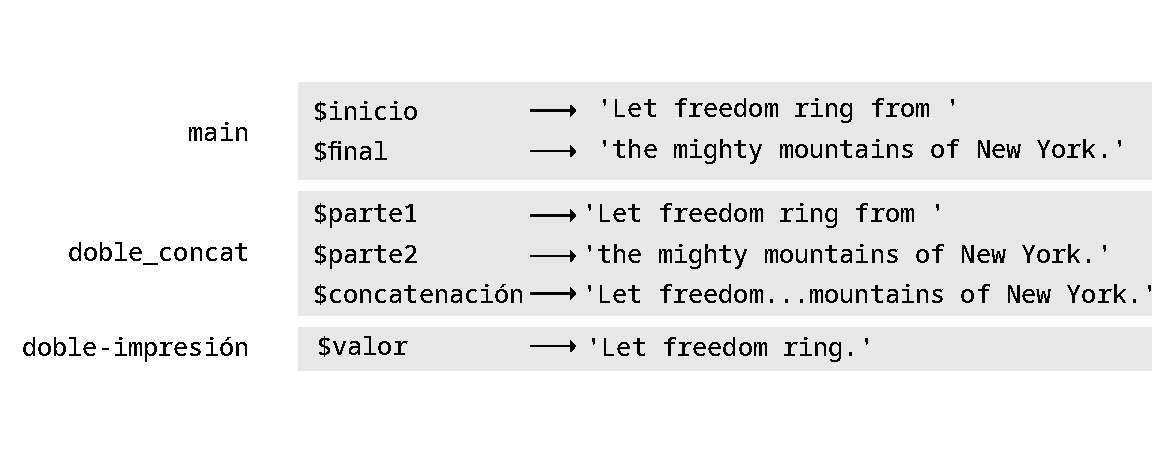
\includegraphics[scale=0.8]{figs/stack_diagram.pdf}}
%{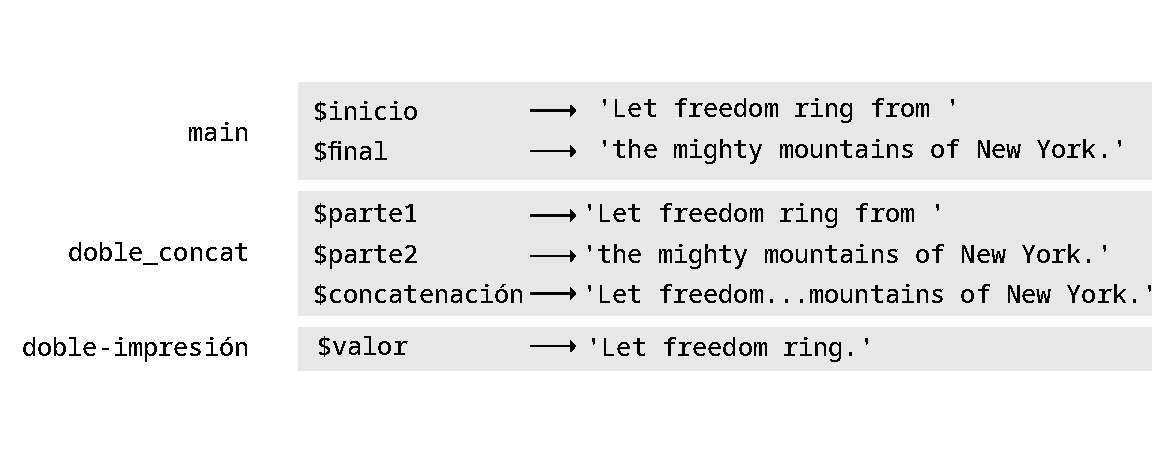
\includegraphics[scale=1.2]{figs/stack_diagram.png}}
\caption{Diagrama de estado.}
\label{fig.stack}
\end{figure}

Los marcos están organizados en la pila para indicar cual función
llama a cual. En este ejemplo, \verb|doble-impresión| fue llamada
por \verb|doble_concat|, y \verb|doble_concat| fue llamada por 
\verb|main|, el cual es un nombre especial para el marco superior.
Cuando creas una variable fuera de cualquier función, dicha variable
le pertenece a \verb|main|.

Cada parámetro hace referencia al mismo valor que su argumento correspondiente.
Así que, {\tt \$parte1} tiene el mismo valor que {\tt \$inicio},
{\tt \$parte2} tiene el mismo valor que {\tt \$final} y {\tt \$valor}
tiene el mismo valor que {\tt \$concatenación}.



\section{Funciones Fructuosas y Funciones Voids}
\index{fruitful function}
\index{void function}
\index{function, fruitful}
\index{function, void} 

Algunas de las funciones que hemos usados, tal como las 
funciones matemáticas, devuelven resultados y son útiles
en cuanto podamos usar el valor devuelto; por falta de un 
mejor nombre, las podamos llamar {\bf funciones fructuosas}.
Otras funciones, tal como \verb|doble-impresión|, realizan una
acción pero no parecen devolver un valor (aunque en verdad devuelve
un valor, {\tt True}, pero no estamos interesados en este valor).
Estas funciones son algunas veces llamadas funciones vacías o funciones
void en otros lenguajes de programación.

En algunos lenguajes de programación, tales como Pascal o Ada,
existe una gran distinción entre una \emph{función} (la cual
devuelve un valor) y un \emph{procedimiento} (el cual no devuelve
ningún valor); ellas son definidas con diferentes palabras claves.
Dicha distinción no aplica en Perl y en la mayoría de los 
lenguajes de programación modernos.

De hecho, desde un punto de vista sintáctico, las funciones de Perl
siempre devuelven un valor. Así que la distinción entre una función
``fructuosa`` y ``void`` no existe sintáctica, solo semánticamente, i.e.,
desde el punto de vista del significado del programa: tal vez necesitamos
usar el valor devuelto, o tal vez no.

Otra distinción que se hace comúnmente entre funciones y mutadores es
que las funciones no cambian el estado inicial de los argumentos 
que se les pasa mientras que los mutadores modifican los argumentos. 
No usaremos esta distinción aquí, pero es útil mantenerla presente.

Cuando llamas una función fructuosa, es muy común que quieras
hacer algo con el resultado; por ejemplo, podrías asignarlo a una
variable o usarlo como parte de una expresión:
 
\begin{lstlisting}
my $altura = sin $radianes;
my $aúreo = (sqrt(5) + 1) / 2;
\end{lstlisting}
%
Cuando llamas una función en el modo interactivo (en
el REPL), Perl usualmente muestra el resultado inmediatamente:

\begin{lstlisting}
> sqrt 5;
2.23606797749979
\end{lstlisting}
%
!`Pero en un script, si llamas una función fructuosa por sí misma,
el valor de retorno se pierde para siempre! En algunos casos, el 
compilador será capaz de advertirte, pero no siempre. Por ejemplo,
considera el siguiente programa:

\begin{lstlisting}
my $cinco = 5;
sqrt $cinco;
say $cinco;
\end{lstlisting}

Este ejemplo produce la siguiente advertencia:

\begin{lstlisting}
WARNINGS for /home/Laurent/perl6_tests/sqrt.pl6:
Useless use of "sqrt $cinco" in expression "sqrt $cinco" in sink context (line 2)
5
\end{lstlisting}
%
El script computa la raíz cuadrada de 5, pero 
dado que no almacena o muestra el resultado, no es muy útil.
\index{interactive mode}
\index{script mode}

Funciones void muestran algo en la pantalla, guardan algún dato
en un archivo, modifican una variable o un objeto, o tienen
algún otro efecto, pero generalmente no tienen un valor de
retorno, o por lo menos algo no muy útil. Si asignas el resultado
a una variable, puedes conseguir el valor de retorno de la subrutina,
el valor de la última expresión que fue evaluada en la función,
o un valor especial tal como {\tt Any}, el cual esencialmente se
refiere a algo que no ha sido definido, o {\tt Nil}.
\index{Any special value}
\index{special value!Any}
%

Las subrutinas que hemos escrito hasta ahora esencialmente muestran cosas
en la pantalla. En ese caso, ellas devuelven {\tt True}, por lo
menos cuando la impresión fue exitoso. Aunque ellas devuelven un 
valor verdadero, lo que ellas devuelven no es muy útil y podemos
considerarlas funciones void para nuestro propósitos.

El siguiente es un ejemplo de una subrutina fructuosa bien simple:
\index{return}

\begin{lstlisting}
> sub cuadrado($número) { return $número ** 2 }
sub cuadrado ($número) { #`(Sub|118134416) ... }
> say cuadrado 5;
25
\end{lstlisting}

El mensaje \verb'Sub|118134416' mostrado por el REPL
es solo un identificador interno de la subrutina que hemos
definido.

La sentencia {\tt return} le indica a la función que termine
la ejecución de la función en esta sentencia y devuelva el valor 
de la siguiente expresión a donde fue llamada. En tal caso 
donde el programa está ejecutando la última sentencia de una 
función, la palabra clave return puede ser omitida dado que la
función devolverá el valor de la última sentencia evaluada,
así que la subrutina {\tt cuadrado} podría ser escrita de 
la siguiente manera:
\begin{lstlisting}
sub cuadrado($número) { 
    $número ** 2 
}
\end{lstlisting}

Usaremos funciones fructuosas más extensivamente en los 
siguientes capítulos.

\section{Signaturas de Funciones}
\index{function!signature}
\index{signature}

Cuando una función recibe argumentos, los cuales son
almacenados en los parámetros, la parte de la definición
de función que describe los parámetros entre los 
paréntesis se llama la {\bf signatura de la función}. Las 
signaturas de funciones que hemos visto hasta ahora son bien 
simple y consisten de un solo parámetro o posiblemente
una lista de parámetros.

Las signaturas pueden proveer una plétora de información
sobre los parámetros usados por la función. Primero, puedes
definir el tipo de los parámetros. Algunas funciones hacen 
sentido solo si sus parámetros son numéricos y deberían
probablemente levantar un error si ellas reciben una
cadena de texto que no pueden ser convertida a un valor
numérico. Por ejemplo, si defines una función {\tt mitad}
que computa el valor igual a su argumento divido por 2,
no hace sentido tratar de computar la mitad de una
cadena de texto que no es numérica. Dicha función
podría escribirse así:
\index{type!parameter}
\index{parameter type}

\begin{lstlisting}
sub mitad(Int $número) { 
    return $número / 2 
}
say mitad 84; # -> 42
\end{lstlisting}

Si está función es llamada con una cadena de texto,
conseguimos el siguiente error:
\index{type!String}

\begin{lstlisting}
> say mitad "Douglas Adams"
===SORRY!=== Error while compiling <unknown file>
Calling mitad(Str) will never work with declared signature (Int $number)
at <unknown file>:1
------> say <HERE>mitad "Douglas Adams"
\end{lstlisting}

El tipo {\tt Int} incluido en la signatura de la función es
una restricción de tipo que puede ayudar a prevenir errores
sutiles. En algunos casos, también pueden ser una molestia.
Considera el fragmento de código:
\index{constraint!type}
\index{type!constraint}
\index{type!Int}
\index{signature}


\begin{lstlisting}
sub mitad(Int $número) {  $número / 2 }
say mitad "84"; # -> ERROR
\end{lstlisting}

Dado que el argumento de la subrutina {\tt mitad} es {\tt "84"},
i.e., una cadena de texto, este código fallará con un error de 
tipo. Si no hubiésemos incluidos el tipo {\tt Int} en la signatura,
el script habría convertido (o \emph{coaccionado}) la cadena de
texto "84" en un número, dividido por 2, y mostrado el
resultado esperado:
\index{type!String}
\index{type!coercion}
\index{coercion!type}

\begin{lstlisting}
sub mitad($número) { $número / 2 }
say mitad "84"; # -> 42
\end{lstlisting}

En algunos casos, tu quieres que esta conversión ocurra,
en otras, no quieres. Es tu deber decidir si quieres
tipado estricto o no, dependiendo en la
situación específica y necesidad. Es probablemente útil usar 
tipos en los parámetros en muchos casos, pero puede 
volverse un obstáculo en algunas situaciones. Perl~6 te deja 
decidir qué tan estricto deseas ser sobre estas cosas.

Nuestra subrutina original {\tt mitad} tiene otra limitación: 
solo funciona con números enteros. Pero una función que 
devuelve la mitad de su argumento debería supuestamente
ser útil para números racionales o hasta otros números. 
Puedes usar los tipos {\tt Real}  o {\tt Numeric} para
hacer la función más general (la diferencia entre los
tipos  es que el tipo {Numeric} aceptará no solo números
{\tt Real}es pero también números complejos ({\tt Complex})
\footnote{~Los números complejos son un concepto matemático
poderoso. Ellos son números de la forma $a + bi$, donde 
$a$ y $b$ son un números reales y $i$ es un número imaginario
de tal modo que $i²$ es igual a $-1$.}). Como sucede con
números complejos, el elegir un tipo {\tt Numeric} abre más 
posibilidades:
\index{Numeric type}
\index{type!Numeric}
\index{Real type}
\index{type!Real}
\index{Complex type}
\index{type!Complex}
\index{type!Int}

\begin{lstlisting}
sub mitad(Numeric $número) { $número / 2 }
say mitad(3+4i); # -> 1.5+2i
\end{lstlisting}

La siguiente tabla resume e ilustra  algunos de los varios
tipos que hemos visto hasta ahora.

\begin{center}
\begin{tabular}{|l|c|}  \hline
\label{types}
\emph{Tipo} & \emph{Ejemplo}   \\ \hline
String      & \verb'"Una cadena de texto (string)"', \verb"'Hola'", \verb'"42"' \\ \hline
Integer     & \verb' -3, -2, 0, 2, 42' \\ \hline
Rational    & \verb' 1/2, 0.5, 3,14159, 22/7, 42.0' \\ \hline
Real        & $\pi$, pi, $\surd{2}$, \emph{e}, $\log 42$, $\sin 0.7$\\ \hline
Complex     & $5.4 + 3i$ \\ \hline
\end{tabular}
\end{center}
\index{String type}
\index{type!String}


\section{Parámetros Inmutables y Mutables}

\index{immutable parameter}
\index{mutable parameter}
\index{parameter!mutable}
\index{parameter!immutable}
Por defecto, los parámetros de una subrutina son apodos {\bf inmutables}
para los argumentos pasados a la subrutina. En otras palabras,
ellos no pueden ser cambiados dentro de la función y tú no puedes
modificar el argumento accidentalmente donde la función es llamada:

\begin{lstlisting}
sub más-tres(Int $número) { $número += 3}
my $valor = 5;
say más-tres $valor; # ERROR: Cannot assign to an immutable value
\end{lstlisting}

En algunos otros lenguajes, este comportamiento es conocido
como una ``llamada por valor``: en términos generales, 
la subrutina recibe (por defecto) un valor y no una variable, y 
el parámetro por lo tanto no puede ser modificado.
\index{call by reference}

Si quieres cambiar el valor del parámetro dentro de la subrutina
(pero sin cambiar el argumento), tú puedes agregar el \emph{trait} 
{\tt is copy} a la signatura:
\index{signature}
\index{trait}
\index{is copy trait}
\index{trait!is copy}

\begin{lstlisting}
sub más-tres(Int $número is copy) { $número += 3}
my $valor = 5;
say más-tres $valor;  # 8
say $valor;             # 5 (valor de la variable intacto)
\end{lstlisting}
%
Un {\bf trait} (rasgo) es una propiedad del parámetro definida
al tiempo de compilación. Aquí, el parámetro {\tt \$número} es
modificado dentro de la subrutina y el valor incrementado es devuelto e 
imprimido como 8, pero, dentro de la función que hace la llamada,
la variable usada como un argumento para la función, {\tt \$valor},
no es modificada (es todavía 5).

Aunque esto puede ser algunas veces peligroso, tú puedes 
también querer escribir una subrutina que modifica su argumento
en el lugar donde la función es llamada. Para esto, puedes usar
el \emph{trait} {\tt is rw} en la signatura:
\index{is rw trait}
\index{trait!is rw}

\begin{lstlisting}
sub más-tres(Int $número is rw) { $número += 3}
my $valor = 5;
say más-tres $valor;  # 8
say $valor;             # 8 ($valor es modificada)
\end{lstlisting}
%
Con el trait {\tt is rw}, el parámetro {\tt \$número} está ahora
\emph{vinculado} al argumento {\tt \$valor}, así que cualquier
cambio hecho al usar {\tt \$número} dentro de la subrutina será 
inmediatamente aplicado a {\tt \$valor} en lugar donde la función
es llamada,porque {\tt \$número} y {\tt \$valor} son solo nombres
diferentes para la misma cosa (ambos hacen referencia a la misma
dirección de memoria). El argumento es ahora totalmente \emph{mutable}.

En algunos otros lenguajes de programación, esto se conoce como
``llamada por referencia``, porque, en aquellos lenguajes, 
si tu pasas una referencia (o un puntero) de una variable a una
función, entonces es posible que la función pueda modificar la
variable referida por la referencia.
\index{call by reference}


\section{Funciones y Subrutinas: Ciudadanos de Primera Clase}
\index{first-class object}
\index{object, first-class}
\index{function!higher-order}
\label{first_class}

Las subrutinas y otros objetos de código se pueden pasar como 
los valores, como cualquier variable, literal u objeto. Entonces
se dice que las funciones son {\bf objetos de primera clase} o algunas
veces, ciudadanos de primera clase o funciones de orden superior. 
Esto significa que una función de Perl (no el valor que devuelve sino
su código) es un valor que puedes asignar a una variable o pasarlo como
un argumento. Por ejemplo, \verb|do-twice| es una subrutina que toma
una función como argumento y la llama dos veces:

\begin{lstlisting}
sub do-twice($código) {
    $código(); 
    $código();
}
\end{lstlisting}

Aquí, el parámetro \verb|$código| se refiere a una función o cualquier
otro objeto que se pueda llamar. Esto es un ejemplo que usa \verb|do-twice|
para llamar una función llamada \verb|saludar| dos veces:

\begin{lstlisting}
sub saludar {
    say "!`Hola Mundo!";
}
do-twice &saludar;
\end{lstlisting}

Esto imprimirá:
\begin{lstlisting}
!`Hola Mundo!
!`Hola Mundo!
\end{lstlisting}

El sigilo \verb|&| se coloca antes del nombre de la subrutina 
en la lista de argumentos para dejarle saber a Perl que estás
pasando una subrutina o cualquier objeto de código 
que se puede llamar (y no estás llamando la
subrutina en el momento).
\index{sigil}
\index{ampersand sigil}
%\index{$&$ sigil}
%\index{sigil!$&$}

De hecho, sería más idiomático usar también el sigilo \verb|&|
en la definición de la subrutina \verb|do-twice| para especificar
que el parámetro es un objeto de código que se puede llamar:
\index{idiomatic}

\begin{lstlisting}
sub do-twice(&código) {
    &código(); 
    &código();
}
\end{lstlisting}

De igual manera:
\begin{lstlisting}
sub do-twice(&código) {
    código(); 
    código();
}
\end{lstlisting}

La sintaxis con el sigilo \verb|&| tiene el beneficio de
proveer un mejor mensaje de error si cometes un error y le pasas
a \verb|do-twice| algo que no se puede llamar. 

Todas las funciones que hemos vistos hasta ahora han tenido nombre,
pero no es necesario que una función tenga un nombre y por lo tanto,
puede ser una función {\bf anónima}. Por ejemplo, 
se puede almacenar directamente en una variable escalar:
\index{anonymous function}
\index{function!anonymous}

\begin{lstlisting}
my $saludar = sub {
    say "!`Hola Mundo!";
};
$saludar();               # imprime "!`Hola Mundo!"
do-twice $saludar;        # imprime "!`Hola Mundo!" dos veces
\end{lstlisting}

Se podría argumentar que la subrutina \verb|$saludar| no es realmente
anónima, debido a que está almacenada en una variable escalar 
que podría de alguna manera ser considerada su nombre. Pero realmente
la subrutina no posee un nombre; solo sucede que está asignada a una
variable escalar. Para demostrar que la subrutina no tiene nombre 
alguno, considera lo siguiente:

\begin{lstlisting}
do-twice(sub {say "!`Hola Mundo!"} );
\end{lstlisting}

Esto imprimirá "!`Hola Mundo!" sin ningún problema. Si la función
\verb|do-twice| se ha declarado posteriormente, puedes hasta 
simplificar la sintaxis y omitir los paréntesis:

\begin{lstlisting}
do-twice sub {say "!`Hola Mundo!"};
\end{lstlisting}

Para casos simples donde no hay necesidad de pasar un argumento
o devolver un valor, puedes omitir la palabra clave \verb|sub|
y pasar un bloque de código directamente a la función:
\index{code block}

\begin{lstlisting}
do-twice {say "!`Hola Mundo!"};
do-twice {say "!`Buen día!"};
\end{lstlisting}

Como puedes observar, \verb|do-twice| es una subrutina \emph{genérica}
cuyo trabajo es ejecutar dos veces cualquier función o bloque
de código que se le pasa, sin ningún conocimiento sobre lo que la 
función o el bloque de código hace. Este es un concepto poderoso
usado en algunas técnicas de programación avanzadas que discutiremos
más adelante.
\index{generic subroutine}

Las subrutinas se pueden también pasar como valores de
retorno desde otras subrutinas:
\index{factory, function}
\index{function!factory}

\begin{lstlisting}
> sub crear-función ($persona) { return sub { say "!`Hola $persona!"}}
# Crear dos funciones de saludos
sub crear-función ($persona) { #`(Sub|176738440) ... }
> my $saludar_mundo = crear-función "Mundo";
sub () { #`(Sub|176738592) ... }
> my $saludar_amigo = crear-función "querido amigo";
sub () { #`(Sub|176739048) ... }
# Usar las funciones de saludos
> $saludar_mundo();
!`Hola Mundo!
> $saludar_amigo();
!`Hola querido amigo!
\end{lstlisting} 

Aquí, la función \verb|crear-función| devuelve una subrutina que saluda
a alguien. Se llama dos veces con dos argumentos diferentes para crear
dos funciones diferentes al tiempo de ejecución, \verb|$saludar_mundo|
y \verb|$saludar_amigo|. Una función como \verb|crear-función| es algunas
veces conocida como una \emph{factoría de funciones} porque puedes crear 
un número determinado de funciones con solo llamar a \verb|crear-función|. Este 
ejemplo puede parecer una manera complicada de hacer algo tan simple. 
Lo que pasa es que en este momento es muy prematuro dar ejemplos útiles,
no obstante esta es una técnica de programación muy poderosa.

Regresaremos a estas técnicas a lo largo de este libro y hasta dedicaremos
un capítulo entero (capítulo~\ref{functional programming}) 
para este asunto y otros temas relacionados.


\section{?`Por qué Funciones y Subrutinas?}
\index{function, reasons for}

Debido a que no está claro el por qué de dividir un programa
en funciones o subrutinas, aquí discutimos varias razones:

\begin{itemize}

\item La creación de una subrutina nueva te da la oportunidad
de nombrar un grupo de sentencias, lo cual hace tu programa más
fácil de leer y depurar. Las subrutinas también ayudan a hacer el 
flujo de ejecución más claro para el lector.

\item Las subrutinas pueden reducir el tamaño de un programa
al eliminar código repetitivo. Más adelante, si haces un cambio,
solamente tienes que hacerlo en un solo lugar.
\index{code repetition}

\item La división de un programa largo en subrutinas te permite
depurar las partes una a una y después ensamblarlas en un todo
que funciona.

\item Las subrutinas que son bien diseñadas usualmente son 
útiles para muchos programas. Una vez que escribes y depuras una,
la puedes reusar.
\index{code reuse}
\index{abstraction}

\item La creación de subrutinas es una de las maneras más
útiles de descomponer un problema difícil en tareas pequeñas 
más fáciles y de crear capas sucesivas de abstracción, las cuales
son las llaves para resolver problemas complejos.
\index{abstraction}

\index{black box}
\item Escribir buenas subrutinas te permite crear cajas negras,
con una entrada y una salida conocida. Así que no tienes que pensar
sobre ellas cuando trabajas en algo más. Se han convertido en
herramientas. Una vez que ensamblas un taladro, no necesitas 
pensar sobre cómo trabaja internamente cuando lo usas para construir
o reparar algo.
\index{black box}

\item En el mundo actual de código abierto, existe la oportunidad
que tu código tendrá que ser comprendido, mantenido or mejorado por 
otras personas. La programación se ha vuelto más y más una actividad
social y la descomposición de tu código en pequeñas subrutinas cuyo
propósito es fácil de entender hará el trabajo de las otras personas
más fácil. Y tú estarás más deleitado cuando la persona que tenga
que mantener o refactorizar tu código sea... tú.  
\index{open source code}

\end{itemize}


\section{Depuración de Programas}

Una de las más importantes habilidades de programación 
que tú adquirirás es la depuración. Aunque algunas veces 
puede ser frustrante, la depuración es una de las partes más
intelectualmente rica, estimulante e interesante de la
programación.  
\index{experimental debugging}
\index{debugging!experimental}

En alguna forma, la depuración se parece al trabajo detectivesco.
Eres confrontado con pistas y debes inferir los procesos y eventos
que conllevaron a los resultados que ves.

La depuración es como una ciencia experimental. Una vez que tienes
una idea de lo que no funciona, modificas el programa e intentas 
nuevamente. Si la hipótesis era correcta, puedes predecir el resultado
de la modificación, y te acercas más a un programa que funciona. Si la
hipótesis era incorrecta, tienes que producir una nueva hipótesis. 
Como Sherlock Holmes señaló, ``Cuando todo aquello que es imposible 
ha sido eliminado, lo que quede, por muy improbable que parezca, 
es la verdad`` (A. Conan Doyle, {\em El signo de los cuatro}).
\index{Holmes, Sherlock}
\index{Conan Doyle, Arthur}

En los casos donde no eres capaz de producir una hipótesis
sobre lo que no funciona, puedes intentar introducir
código del cual espera un determinado tipo de error, 
una ``hipótesis negativa``. Algunas veces puedes aprender 
mucho del hecho de que no creó el error que se esperaba. 
Crear una hipótesis no significa necesariamente que tienes 
una idea sobre cómo hacerlo funcionar, también podría ser
una hipótesis sobre cómo hacerlo fallar.

Para algunas personas, la programación y la depuración son
la misma cosa. Es decir, la programación es el proceso de 
depurar gradualmente un programa hasta que hace lo que quieres.
La idea es que tú deberías comenzar con un programa que funciona y 
hacer pequeñas modificaciones, y depurarlas según avanzas.

Por ejemplo, Linux es un sistema operativo que contiene millones 
de líneas de código. Sin embargo, todo comenzó con un simple programa
que Linus Torvalds usó para explorar el chip Intel 80386. De acuerdo
a Larry Greenfield, "Uno de los proyectos iniciales de Linus fue un 
programa que cambiaba entre la impresión de \verb|AAAA| y \verb|BBBB|.
Luego éste evolucionó en Linux.``
({\em The Linux Users' Guide} Beta Version 1).
\index{Linux}


\section{Glosario}

\begin{description}

\item[Función] Una secuencia de sentencias que realiza 
una función útil. Las funciones pueden cero o más argumentos
y pueden producir o no producir un resultado. Perl viene con 
muchas funciones integradas, y tú puedes crear tus propias
funciones. En Perl, las funciones definidas por el usuario son
usualmente conocidas como subrutinas.
\index{function}

\item[Definición de una función]  Una sentencia que crea una función
nueva, especifica su nombre, sus parámetros, y las sentencias
que contiene.
\index{function!definition}

\item[Cabecera] La primera línea de la definición de la 
función.
\index{header}

\item[Cuerpo] La secuencia de sentencias dentro de la definición
de la función, usualmente en un bloque de código delimitado por
llaves.
\index{body}

\item[Parámetro] Un nombre que usa dentro de la subrutina
para referirse al valor que se pasa como un argumento.
\index{parameter}

\item[Llamada de función] Una sentencia que ejecuta la función.
Consiste del nombre de la función seguido por una lista de 
argumentos, la cual puede o no puede estar encerrada por
paréntesis.
\index{function!call}

\item[Argumento] Una valor que se provee a la función cuando
ésta se llama. Este valor es asignado al parámetro 
correspondiente en la función.
\index{argument}

\item[Variable lexical] Una variable definida dentro de una
subrutina o un bloque de código. Una variable lexical definida
dentro de una función se puede usar solo dentro de la función.
\index{local variable}

\item[Valor de retorno]  El resultado de una función. Si una llamada
de función se usa como una expresión, el valor de retorno es el valor 
de la expresión.
\index{return!value}

\item[Any]  Una valor especial típicamente encontrado en 
las variables a las cuales no se le ha asignado un valor. Es 
también un valor especial devuelto por algunas funciones que 
llamamos ``void`` (porque ellas devuelven algo que no es
generalmente útil tal como ``Any``).
\index{Any special value}
\index{special value!Any}

\item[Nil] Tambié un valor especial devuelto algunas veces
 por las subrutinas ``void``.

\item[Módulo] Una archivo que contiene una colección
de funciones relacionadas y otras definiciones.
\index{module}

\item[Sentencia use] Una sentencia que lee un módulo y 
usualmente exporta algunas funciones.
\index{use statement}
\index{statement!use}

\item[Composición] Usar una expresión como parte de
una expresión más compleja o una sentencia como parte
de una sentencia más larga.
\index{composition}

\item[Flujo de ejecución]  El orden en cual las sentencias
son ejecutadas.
\index{flow of execution}

\item[Diagrama de pila]  Una representación gráfica de una
pila de subrutinas, sus variables, y los valores a los cuales
hacen referencia.
\index{stack diagram}

\item[Marco]  Una caja en un diagrama de pila que representa una
llamada de subrutina. Contiene las variables locales y los 
parámetros de la subrutina.
\index{function!frame}
\index{frame}

\item[Función fructuosa] Una functión que devuelve un valor
útil.
\index{fruitful function}

\item[Funcción void] Una función o subrutina que no devuelve
un valor útil.
\index{void function}

\item[Signatura de una función] La parte de la definición de 
una función (usualmente entre paréntesis) que define 
sus parámetros y posiblemente sus tipos y otras propiedades.
\index{function!signature}
\index{signature}

\item[Parámetros inmutables] Una parámetro de una función
o subrutina que no se puede cambiar dentro del cuerpo de
la función. Por defecto, los parámetros de una
subrutinas son inmutables.
\index{immutable parameter}

\item[Trait] Una propiedad de un parámetro de una función
o subrutina que es definido al tiempo de compilación.
\index{trait}

\item[Objeto de primera clase] Las subrutinas de Perl se
dice que son objetos de orden superior o objetos de primera 
clase porque ellas se pueden pasar como argumentos a 
otras subrutinas o como valores de retorno, como cualquier
otro objeto.
\index{first-class object}
\index{object, first-class}

\item[Función anónima] Una función que no tiene nombre.
\index{anonymous function}
\index{function!anonymous}

\item[Factoría de funciones] Una función de produce otras 
funciones como valores de retorno.
\index{factory, function}
\index{function!factory}

\end{description}


\section{Ejercicios}

\begin{exercise}
\index{chars function}
\index{function!chars}
\label{right_justify}

Escribe una subrutina llamada \verb|alinear-a-derecha| 
que toma una cadena de texto llamada {\tt \$cadena-entrada}
como parámetro e imprime la cadena de texto con suficiente
espacio blanco de tal modo que la última letra de la cadena
de texto esté en la columna 70 de la pantalla.

\begin{lstlisting}
> alinear-a-derecha('Larry Wall')
                                                           Larry Wall
\end{lstlisting}

Pista: Usa la concatenación de cadena de texto y repetición. 
De igual manera, Perl provee una función integrada llamada 
{\tt chars} que devuelve la longitud de una cadena, así que
el valor de \verb"chars 'Larry Wall'" or \verb"'Larry Wall'.chars"
es 10. Solución: \ref{sol_right_justify}.

\end{exercise}


\begin{exercise}
\index{first-class object}
\index{object!first-class}
\index{do-twice}
\label{do_it_twice}

Hemos visto que las funciones y otros objetos de código 
se pueden pasar como valores, tal como cualquier objeto. Se dice
que las funciones \emph{objetos de primera clase}. Por ejemplo, 
\verb|do-twice| es una función que toma una función como un
argumento y la llama dos veces:

\begin{lstlisting}
sub do-twice($código) {
    $código(); 
    $código();
}
sub saludar {
    say "Hello World!";
}
do-twice(&saludar);
\end{lstlisting}

\begin{enumerate}

\item Escribe este ejemplo en un script y 
pruébalo.

\item Modifica la función \verb|do-twice| para que tome
dos argumentos, una función y un valor, y llama la función
dos veces, pasando el valor como una argumento.

\item Copia la definición de \verb|doble-impresión| del 
inicio de este capítulo en tu script.

\item Usa la versión modificada de \verb|do-twice| para llamar
a \verb|doble-impresión| dos veces, pasando como argumento
la cadena de texto ``What's up doc''.

\item Define una función nueva llamada \verb|do-four|
que toma una función y un valor y llama la función
cuatro veces, pasando el valor como un argumento. Deberían
haber solo dos sentencias en el cuerpo de la función, no cuatro.

\end{enumerate}

Solución: \ref{sol_do_it_twice}.

\end{exercise}



\begin{exercise}
\label{draw_a_grid}
\index{print-grid}

Nota: Debes resolver este ejercicio con solo el uso de
las sentencias y otras características que hemos
discutidos hasta ahora.

\begin{enumerate}

\item Escribe una subrutina que dibuje una cuadrícula como 
la siguiente:
\index{grid}

\begin{lstlisting}
+ - - - - + - - - - +
|         |         |
|         |         |
|         |         |
|         |         |
+ - - - - + - - - - +
|         |         |
|         |         |
|         |         |
|         |         |
+ - - - - + - - - - +
\end{lstlisting}
%
Pista: para imprimir más de un valor en una línea, puedes
imprimir una secuencia de valores separados por coma:

\begin{lstlisting}
  say '+', '-';
\end{lstlisting}
%
La función {\tt say} imprime sus argumentis con una nueva línea
al final (la cual avanza el cursor a la siguiente línea). Si no
quieres colocar el cursor en la siguiente línea, entonces usa
la función {\tt print}:

\begin{lstlisting}
  print '+', ' ';
  print '-';
\end{lstlisting}
%
La salida de estas sentencias es ``+ -''.

Una sentencia {\tt say} con una cadena de texto vacía como
argumento termina la actual línea y va a la siguiente
línea.

\item Escribe una subrutina que dibuje una cuadrícula similar con
cuatro filas y cuatro columnas.

\end{enumerate}

Solución: \ref{sol_draw_a_grid}
\index{print-grid}.

Crédito: Este ejercicio está basado en un ejercicio en Oualline, {\em
    Practical C Programming, Third Edition}, O'Reilly Media, 1997.

\end{exercise}



\chapter{Bucles, Condicionales, y Recursión}
\label{conditionals}

El tema principal de  este capítulo es la sentencia {\tt if},
la cual ejecuta código diferente dependiendo del estado
del programa. Pero primero quiero introducir dos operadores
nuevos: división de enteros y módulo.


\section{División de Enteros y Módulo}

El operador {\bf división de enteros}, \verb"div", 
divide dos números y los redondea a un entero. Por ejemplo,
supón que una película se tarda 105 minutos. Podrías querer
saber cuántas horas hay en 105 minutos. En Perl, la división
convencional devuelve un número racional (en muchos lenguajes,
devuelve un número de coma flotante, que es otra forma
de representación interna de números que no son enteros):

\begin{lstlisting}
> my $minutos = 105;
> $minutos / 60;
1.75
\end{lstlisting}

Sin embargo, normalmente nosotros no escribimos las horas con
puntos decimales. La división de enteros devuelve el número
entero de horas, descartando la parte fraccional:
\index{operator!div}
\index{div operator}
\index{integer division}

\begin{lstlisting}
> my $minutos = 105;
> my $horas = $minutos div 60;
1
\end{lstlisting}

En aritmética, la división de enteros es algunas veces
llamada \emph{división euclidiana}, la cual calcula el
cociente y el residuo.
\index{Euclidean division}
\index{division remainder}

Para conseguir el residuo, podrías sustraer una hora en 
minutos:

\begin{lstlisting}
> my $residuo = $minutos - $horas * 60;
45
\end{lstlisting}

\index{integer division}
\index{floating-point division}
\index{division!integer}
\index{division!floating-point}
\index{modulo operator}
\index{operator!modulo}

Una alternativa es usar el {\bf operador de módulo}, \verb|%|,
el cual divide dos números y devuelve el residuo:
%\index{$%$ modulo operator}
%\index{operator!$%$ (modulo)}

\begin{lstlisting}
> my $residuo = $minutos % 60;
45
\end{lstlisting}
%
El operador de módulo es muy común en los lenguajes de programación
y es más útil de lo que parece. Por ejemplo, puedes chequear si
un número es divisible por otro---si {\tt \$dividendo \% \$divisor} es cero, entonces {\tt \$dividendo} es divisible por {\tt \$divisor}. 
Esto es usado comúnmente, por ejemplo, con un divisor igual a 2 para determinar si un número es par o impar. Veremos un ejemplo
de esto más adelante en este capítulo (ver Sección~\ref{alternative.execution}).
\index{divisibility}
\index{even number}
\index{odd number}
\index{integer!even}
\index{integer!odd}

Para ser sincero, Perl~6 también tiene un operador específico 
para la divisibilidad, \verb|%%|. La expresión
\verb|$dividendo %% $divisor| devuelve verdadero si 
\verb|$dividendo %% $divisor| es igual a 0,
es decir si {\tt \$dividendo} es divisible por {\tt \$divisor} 
(de lo contrario, es falso):
\index{divisibility!operator}
\begin{lstlisting}
> 42 %% 2;
True
\end{lstlisting}

De igual manera, puedes extraer el dígito más a la
derecha o dígitos de un número con el operador
de módulo. Por ejemplo, {\tt \$x \% 10}  extrae el
dígito más a la derecha de {\tt \$x} (en base 10).
Similarmente, {\tt \$x \% 100} extrae los últimos dos 
dígitos:

\begin{lstlisting}
> 642 % 100;
42
\end{lstlisting}
%
\index{modulo operator}
\index{operator!modulo}



\section{Expresiones Booleanas}
\index{Boolean expression}
\index{expression!Boolean}
\index{logical operator}
\index{operator!logical}

Una {\bf expresión booleana} es una expresión que es
verdadera o falsa. Los siguientes ejemplos usan el operador
{\tt ==} para comparar los operandos numéricos y producir
{\tt True} si son iguales y de lo contrario, {\tt False}:

\begin{lstlisting}
> 5 == 5;
True
> 5 == 6;
False
\end{lstlisting}
%
{\tt True} y {\tt False} son valores especiales
que pertenecen al tipo {\tt Bool}; ellos no son
cadenas de texto:
\index{True!special value}
\index{False!special value}
\index{special value!True}
\index{special value!False}
\index{Bool type}
\index{type!Bool}

\begin{lstlisting}
> say True.WHAT
(Bool)
> say False.WHAT
(Bool)
\end{lstlisting}
%
\index{operator!$==$ (numeric equality)}
\index{$==$ numeric equality operator}
El operador {\tt ==} es uno de los {\bf operadores de relación
numérica} y su función es chequear si los operandos son 
iguales; los otros son:

\begin{lstlisting}
      $x != $y            # $x no es numéricamente igual a $y
      $x > $y             # $x es numéricamente mayor que $y
      $x < $y             # $x es numéricamente menor que $y
      $x >= $y            # $x es numéricamente mayor o igual a $y
      $x <= $y            # $x es numéricamente menor o igual a $y
      $x === $y           # $x y $y son verdaderamente idénticos
\end{lstlisting}
% TODO: get these entries working in plastex
\ifplastex \else
\index{"!= numeric inequality operator@\texttt{"!=} numeric inequality operator}
\index{< less than numeric operator@\texttt{<} less than numeric operator}
\index{> greater than numeric operator@\texttt{>} greater than numeric operator}
\index{>= greater than or equal operator@\texttt{>=} greater than or equal operator}
\index{<= less than or equal operator@\texttt{<=} less than or equal operator}
\index{=== value identity operator@\texttt{===} value identity operator}
\index{operator!"!= (numeric inequality)@\texttt{"!=} (numeric inequality)}
\index{operator!< (numerically less than)@\texttt{<} (numerically less than)}
\index{operator!> (numerically greater than)@\texttt{>} (numerically greater than)}
\index{operator!>= (greater than or equal)@\texttt{>=} (greater than or equal)}
\index{operator!<= (less than or equal)@\texttt{<=} (less than or equal)}
\index{operator!=== (value identity)@\texttt{===} (value identity)}
\fi
Aunque estas operaciones probablemente son familiares, los
símbolos en Perl son diferentes a los símbolos matemáticos.
Un error común es usar un solo signo de igualdad ({\tt =}) en vez de 
dos signos de igualdad ({\tt ==}). Recuerda que {\tt =} es el
operador de asignación y {\tt ==} es un operador de relación.
No existe tal cosa como {\tt =<}, aunque existe el operador {\tt =>},
el cual no es un operador de relación sino algo completamente
distinto (como veremos más adelante, dicho operador es el constructor 
de pares). 
\index{relational operator}
\index{relational operator!numeric}
\index{numeric relational operator}
\index{equality operator}
\index{operator!equal}
\index{operator!relational}
\index{pair constructor}
\index{constructor!pair}
% TODO: get these entries working in plastex
\ifplastex \else
\index{=> pair constructor@\texttt{=>} pair constructor}
\index{operator!=> (pair constructor)@\texttt{=>} (pair constructor)}
\fi

La diferencia entre {\tt ==} y {\tt ==} es que el primer
operador chequea si los valores de los operandos son iguales
y el último chequea si los  operandos son verdaderamente
idénticos. Como un ejemplo, considera esto:

\begin{lstlisting}
say 42 ==  42;           # True
say 42 ==  42.0;         # True
say 42 ===  42;          # True
say 42 === 42.0;         # False
\end{lstlisting}
%

Estos operadores de relación pueden solo comparar 
valores numéricos (números o variables que contienen
números) o valores que se pueden coaccionar en 
valores numéricos, tal como, por ejemplo,
la cadena de texto "42" la cual, si se usa con estos
operadores (excepto {\tt ===}), serán coaccionada 
en el número 42.
\index{coercion}

Para la comparación de cadenas de texto (en un tipo de 
comparación lexicográfica o ``pseudo-alfabética``),
necesitas usar los {\bf operadores de relación de cadena
de texto}:

\begin{lstlisting}
      $x eq $y            # $x es una cadena de texto igual a $y
      $x ne $y            # $x no es una cadena de texto igual a $y
      $x gt $y            # $x es mayor que $y (alfabéticamente después)
      $x lt $y            # $x es menor que $y (alfabéticamente antes)
      $x ge $y            # $x es mayor o igual a  $y
      $x le $y            # $x es menor o igual a  $y
      $x eqv $y           # $x es verdaderamente equivalente a $y
\end{lstlisting}
%  
\index{relational operator}
\index{relational operator!string}
\index{string!relational operator}
\index{operator!relational}
\index{eq, string equality operator}
\index{operator!eq (string equality)}
\index{ne, string inequality operator}
\index{operator!ne (string inequality)}
\index{operator!gt (alphabetically after)}
\index{operator!lt (alphabetically before)}



Por ejemplo, puedes comparar (alfabéticamente) los nombres
de dos presidentes de los Estados Unidos:
\begin{lstlisting}
> 'FDR' eq 'JFK';
False
> 'FDR' lt 'JFK';    # comparación alfabética
True
\end{lstlisting}
%  

A diferencia de otros lenguajes de programación, Perl~6 te permite 
encadenar varios operadores de relación de forma transitiva,
al igual que en notación matemática:

\begin{lstlisting}
say 4 < 7 < 12;      # True
say 4 < 7 < 5;       # False
\end{lstlisting}
\index{chained relational operator}

Es necesario aclarar que los operadores de relación
numérica y los operadores de relación de cadena de texto no 
funciona de la misma manera (y esta es una buena razón 
para tener operadores diferentes), porque ellos no poseen
la misma idea de lo que \emph{mayor que} o \emph{menor que}.

Al comparar dos enteros positivos, un número con cuatro dígitos
es siempre mayor que un número con solo dos o tres dígitos. 
Por ejemplo, 1110 es mayor que 886. 

Por lo contrario, la comparación de cadenas de texto
sigue básicamente reglas (pseudo) alfabéticas: 
``b'' es mayor que ``aaa'', porque la regla comúnmente
aceptada para la comparación de cadenas de texto es
comenzar a comparar la primera letra de cada cadena
de texto: si las dos letras son diferentes se sabe cuál de
las dos cadenas es mayor sin importar el carácter que viene
a continuación; necesitas proceder con la comparación
de la segunda letra de cada palabra solo si la comparación
de la primera letra de cada cadena termina en un empate, etc.
Así que cualquier palabra que inicia con ``a`` es menor que 
cualquier palabra que inicie con ``b``, sin importar la longitud
de estas palabras. Esto puede parecer algo minucioso, no 
obstante esto se vuelve esencial cuando comienzas 
a ordenar elementos: realmente tienes que pensar qué tipo
de orden (numérico o alfabético) quieres usar.
\index{sorting}

También existen los operadores de relación de ``tres sentidos``,
{\tt cmp}, {\tt <=>} y {\tt leg}, pero regresaremos a ellos
cuando estudiemos cómo ordenar los elementos de una lista. 
Similarmente, necesitamos aprender otras cosas sobre Perl antes
que podamos justificar el increíblemente poderoso y expresivo
operador de \emph{coincidencia inteligente}, \verb|~~|.
\index{sorting}
\index{smart match operator}
\index{operator!smart match}
\index{three-way operator}
\index{operator!three-way}
\index{cmp operator}
\index{leg operator}
\index{operator!leg}
% TODO: get these entries working in plastex
\ifplastex \else
\index{<=> operator@\texttt{<=>} operator}
\index{operator!<=> (numeric comparison)@\texttt{<=>} (numeric comparison)}
\fi

Un punto final acerca de la comparación de cadenas
de texto es que las letras mayúsculas son siempre menores
que las letras minúsculas. Así que  "A," "B," "BB," y "C"
son \emph{todas} menores que "a," "b," "bb," y "c".
No discutiremos los detalles aquí pero esto se vuelve
complicado (y algo confuso) cuando las cadenas de texto
a ser comparadas contienen caracteres no alfabéticos (
o letras Unicode que no son ASCII).

\section{Operadores Lógicos}
\index{logical operator}
\index{operator!logical}

Hay tres pares principales de {\bf operadores lógicos}:
\begin{itemize}
\item lógico \emph{and} (y) : ``{\tt and}'' y {\tt \&\&}
\item lógico \emph{or} (o): ``{\tt or}'' y {\tt ||}
\item lógico \emph{not} (no): ``{\tt not}'' y {\tt !}
\end{itemize}

La semántica (significado) de estos operadores es similar
a sus significados en inglés (y en español). Por ejemplo,
{\tt \$x > 0 and \$x < 10} es verdadera solo si {\tt \$x}
es mayor que 0 \emph{and} menos que 10.
\index{and operator}
\index{or operator}
\index{not operator}
\index{operator!and}
\index{operator!or}
\index{operator!not}

{\tt \$n \% 2 == 0 and \$n \% 3 == 0} es verdadero si {\em ambas}
condiciones son verdaderas, es decir, si el número es divisible por
2 \emph{and} por 3, i.e., es de hecho divisible por 6 (que podría
ser mejor escrito así: {\tt \$n \% 6 == 0} or {\tt \$n \%\% 6}).

{\tt \$n \% 2 == 0 or \$n \% 3 == 0} es verdadero si \emph{una o ambas}
condiciones son verdaderas, es decir, si el número es divisible por 2
\emph{or} por 3 (or ambos).

Finalmente, el operador {\tt not} niega una expresión Booleana,
así que {\tt not (x > y)} es verdadero si {\tt x > y} es falso, es
decir, si {\tt x} es menor o igual {\tt y}.

Los operadores {\tt \&\&}, {\tt ||}, y {\tt !} tienen el mismo
significado, respectivamente, como {\tt and}, {\tt or}, y {\tt not},
pero una precedencia más estricta, lo que significa 
que cuando están en una expresión con algunos otros operadores,
ellos tienen una mayor precedencia de ejecución. Volveremos
con la precedencia más adelante, pero digamos por el tiempo
presente que, en los casos más comunes, los operadores 
{\tt and}, {\tt or}, y {\tt not} usualmente serán suficientes
para hacer lo que deseas.
\index{precedence}      
\index{operator precedence}

En sentido estricto, los operandos de los operadores lógicos
deberían ser expresiones Booleanas, pero Perl, como muchos
otros lenguajes derivados parcialmente de C, no es estricto
con respecto a eso. Los números~0 y 0.0 son falsos; y cualquier
número que no sea cero o una cadena de cuerda que no esté 
vacía es interpretado como {\tt True}:

\begin{lstlisting}
> 42 and True;
True
\end{lstlisting}
%
Aunque esta flexibilidad puede ser muy útil, existen 
sutilezas que pueden ser confusas. A menos que sepas
lo que estás haciendo, esto es algo que deberías evitar.

La función integrada {\tt so} devuelve una evaluación 
de sus argumentos:

\begin{lstlisting}
> say so (0 and True);
False
\end{lstlisting}
%
Aquí la expresión {\tt (0 and True)} es falsa porque 0 es falso
y la expresión sería verdadera solo si ambos argumentos del operador
{\tt and} son verdaderos.

Cuando varias condiciones Booleanas son enlazadas con algunos
operadores lógicos, Perl solo realizará la comparaciones que son
estrictamente necesarias para descifrar el resultado final,
comenzando con aquellas en la izquierda. Por ejemplo, si escribes:

\begin{lstlisting}
> False and $número > 0;
False
\end{lstlisting}
%
no hay necesidad de evaluar la segunda expresión Booleana
para saber que la expresión completa será falsa. En este caso,
Perl no trata de chequear si el número es positivo o hasta si
está definido. Se dice que estos operadores realizan una evaluación
de ``cortocircuito`` con las condiciones innecesarias.
\index{short-circuit boolean operators}
\index{short-circuit evaluation}

De la misma manera, en el siguiente código, la subrutina 
{\tt calcular-pensión} no será llamada si la edad de la persona
es menos de 65:

\begin{lstlisting}
$edad >= 65 and calcular-pensión();
\end{lstlisting}
%
Lo mismo ocurre con el operador {\tt or}, pero de
manera completamente distinta: si la primera expresión booleana
de una sentencia {\tt or} es verdadera, entonces la siguiente
expresión no será evaluada. El siguiente código es equivalente
al anterior:

\begin{lstlisting}
$edad < 65 or calcular-pensión();
\end{lstlisting}
% 
Esta \emph{puede} ser una forma de ejecutar la subrutina
{\tt calcular-pensión} condicionalmente, dependiendo del 
valor de la edad, y esto se usa usualmente en construcciones
tal como:

\begin{lstlisting}
haz-algo() or die "no pude hacer algo";
\end{lstlisting}
%
la cual aborta el programa si {\tt haz-algo} devuelve un 
valor falso, lo cual quiere decir que fue incapaz de hacer 
algo tan esencial que no vale la pena continuar con su
ejecución.

Más adelante examinaremos formas más claras y comunes
de ejecutar código con condicionales.

\section{Ejecuciones Condicionales}
\label{conditional.execution}

\index{conditional!statement}
\index{statement!conditional}
\index{if statement}
\index{statement!if}
\index{conditional!execution}
Para escribir programas útiles, casi siempre necesitamos la habilidad 
de evaluar condiciones y cambiar el comportamiento del programa
adecuadamente. Las {\bf sentencias condicionales} nos brindan esta
habilidad. La forma más simple es la sentencia {\tt if}:

\begin{lstlisting}
if $número > 0 {
    say '$número es positivo';
}
\end{lstlisting}
%
La expresión Booleana después de {\tt if} se conoce 
como la condición. Si la condición es verdadera, el
bloque de código subsecuente se ejecuta. Si es falsa, 
nada pasa. El bloque de código puede contener cualquier
cantidad de sentencias.
\index{condition}

Es una convención y muy recomendado (aunque no es mandatario
desde la perspectiva del compilador) indentar las sentencias
del bloque, para así ayudar con la visualización del 
\emph{flujo de control} del programa, i.e., su estructura
de ejecución: con tal indentación, podemos ver mucho mejor 
que las condiciones dentro del bloque serán ejecutadas solo 
si la condición es verdadera.
\index{indentation}

La condición puede ser una expresión Booleana compuesta:
\begin{lstlisting}
if $n > 0 and $n < 20 and $n %% 2 {
    say '$n es un número par y positivo menor que 20'
}
\end{lstlisting}
%
Nota que en la sentencia de impresión anterior, el punto y coma
final se omitió. Cuando una sentencia es la última línea de
código de un bloque, inmediatamente antes de la llave derecha
{\tt \}} que cierra el bloque, el punto y coma final es opcional
y puede ser omitido, aunque sería recomendable incluirlo.
\index{omitting the semi-colon}
\index{semi-colon, omitting}
\index{bracket!curly}
\index{curly bracket}
\index{curly brace}

En teoría, el fragmento de código anterior es por sí mismo una
sentencia y debería también terminar con un punto y coma después
de la llave derecha. Pero una llave derecha seguida por un carácter
de nueva línea implica un separador de sentencia, así que no 
necesitas un punto y coma ahí y por lo tanto, es generalmente
omitido.
\index{omitting the semi-colon}
\index{semi-colon, omitting}



\section{Ejecución Alternativa}
\label{alternative.execution}
\index{alternative execution}
\index{else keyword}
\index{keyword!else}

Una segunda forma de la sentencia {\tt if} es la
``ejecución alternativa``, en la cual existen dos 
posibilidades y la condición determina cual de ellas
ejecutar. Dada una variable \verb|$número| que 
contiene una entero, el siguiente código muestra dos
mensajes diferentes dependiendo si el valor del
entero es par o impar:

\begin{lstlisting}
if $número % 2 == 0 {
    say 'La variable $número es par'
} else {
    say 'La variable $número es impar'
}
\end{lstlisting}
%
\index{even number}
\index{odd number}
\index{integer!odd}
\index{integer!even}
Si el residuo del {\tt \$número} dividido por 2 es 0,
entonces sabemos que el {\tt \$número} es par, y el programa
muestra el mensaje apropiado. Si la condición es falsa,
el segundo conjunto de sentencias se ejecuta. Dado que la
condición debe ser verdadera o falsa, exactamente una de las
alternativas será ejecutada. Las alternativas son conocidas
como {\bf ramas}, por ellas son ramas en el flujo de ejecución.
\index{branch}

Nota que si \verb|$número| divide a dos exactamente, este
código imprimirá:

\begin{lstlisting} 
La variable $número es par
\end{lstlisting}

El valor de la  variable \verb|$número| no es interpolado,
porque hemos usado las comillas simples con el propósito
de imprimir el nombre de la variable y no su valor. Habríamos
usado las comillas inglesas si hubiésemos querido imprimir
el valor de la variable y no el nombre.
\index{single quote}
\index{double quote}
\index{quote!single}
\index{quote!double}
\index{variable!interpolation}
\index{interpolation}


\section{Condicionales Encadenadas}
\index{chained conditional}
\index{conditional!chained}

Algunas veces existen más de dos posibilidades y 
necesitamos más de dos ramas en el flujo de ejecución.
Una forma de expresar una computación como ésta es con
el uso de una {\bf condicional encadenada}:

\begin{lstlisting}
if $x < $y {
    say 'La variable $x es menor que la variable $y'
} elsif $x > $y {
    say 'La variable $x es mayor que la variable $y' 
} else {
    say 'Las variables $x y $y son iguales'
}
\end{lstlisting}
%
La palabra clave {\tt elsif} es una abreviación de ``else if``
que tiene la ventaja de prevenir los bloques anidados. Otra vez,
exactamente una de las ramas será ejecutada. No hay límite 
con el número de sentencias {\tt elsif}.

Si existe una claúsula {\tt else}, tiene que ir al 
final. Sin embargo, no tiene que haber una:

\index{elsif keyword}
\index{keyword!elsif}

\begin{lstlisting}
if $selección eq 'a' {
    draw_a()
} elsif $selección eq 'b' {
    draw_b()
} elsif $selección eq 'c' {
    draw_c()
}
\end{lstlisting}
%
Cada condición es examinada en orden. Si la primera
es falsa, la siguiente es examinada, etc. Si una de ellas
es verdadera, la rama correspondiente se ejecuta y la
sentencia finaliza. Aún si más de una condición es verdadera,
solo la primera rama se ejecuta.


\section{Condicionales Anidadas}
\index{nested conditional}
\index{conditional!nested}

Una condicional puede también ser anidada dentro de otra. Podríamos
haber escrito el ejemplo anterior de la siguiente manera:

\begin{lstlisting}
if $x == $y {
    say 'Las variables $x y $y son iguales'
} else {
    if $x < $y {
        say 'La variable $x es menor que la variable $y'
    } else {
        say 'La variable $x es mayor que la variable $y'
    }
}
\end{lstlisting}
%
La condicional exterior contiene dos ramas. La primera
rama contiene una sentencia simple. La segunda rama contiene
otra sentencia {\tt if}, la cual contiene dos ramas. Estas 
dos ramas son sentencias simples, aunque pudieran haber sido
sentencias condicionales. Se dice que la condición \verb|if $x < $y| 
está anidad dentro de la rama {\tt else} de la condicional
exterior.

Tales condicionales anidadas muestran lo crítico que es 
para tu propia comprensión indentar apropiadamente las
sentencias condicionales, debido a que sería difícil 
entender la estructura sin la ayuda visual
proveída por la correcta indentación.
\index{indentation}

Aunque la indentación de las sentencias ayuda
a entender la estructura, las {\bf condicionales anidadas}
se vuelven difícil de leer bien rápido. Es una buena
idea evitarlas cuando se pueda. Los operadores lógicos
usualmente proveen una manera de simplificar las
condicionales anidadas. Por ejemplo, considera
el siguiente código (el cual asume que \verb|$x| es
un entero):
\index{logical operator}

\begin{lstlisting}
my Int $x;
# ... $x = ...;
if 0 < $x {
    if $x < 10 {
        say 'El valor de $x es un número positivo de un solo dígito.'
    }
}
\end{lstlisting}
%
La sentencia {\tt say} se ejecuta solo si pasamos ambas condicionales,
así que podemos obtener el mismo efecto con el operador Booleano {\tt and},
y el código puede escribirse usando una sola condicional:

\begin{lstlisting}
if 0 < $x and $x < 10 {
    say '$x es un número positivo de un solo dígito.'
}
\end{lstlisting}

Para este tipo de condición, Perl~6 provee una opción más concisa
usando los operadores de relación encadenados discutidos 
anteriormente:

\begin{lstlisting}
if 0 < $x < 10 {
    say '$x es un número positivo de un solo dígito.'
}
\end{lstlisting}
\index{chained relational operator}

\section{Condicionales If como Modificadores de Sentencias}
\index{statement modifier} \index{modifier!statement}
\index{postfix conditional} \index{conditional!postfix }

También existe una forma de {\tt if} conocida como un
{\bf modificador de sentencia} (o algunas veces ``condicional sufija``)
cuando hay solo una sentencia condicional. En este caso, 
la sentencia {\tt if} y la condición vienen después del 
código que quieres ejecutar condicionalmente. Nota que la 
condición es siempre la primera en ser evaluada:

\begin{lstlisting}
say '$número es negativo.' if $número < 0;
\end{lstlisting}
%
Esto es equivalente a:
\begin{lstlisting}
if $número < 0 {
    say '$número es negativo.' 
}
\end{lstlisting}
%
Esta forma sintáctica es más concisa debido a que toma
una sola línea de código en vez de tres. La ventaja de esto
es que puedes ver más de tu código en una sola pantalla,
sin tener que desplazarte hacia arriba o hacia abajo. 
Sin embargo, este sintaxis es nítida y limpia solo cuando
la condición y la sentencia son cortas y simple. Por lo
tanto, es mejor usarlas en estos casos.

El modificador de sentencia no permite el uso de las
sentencias {\tt else} y {\tt elsif}.

\section{Sentencia Condicional Unless}
\index{unless statement}
\index{keyword!unless}

Si no te gusta escribir condiciones negativas en sentencia
condicional {\tt if} tal como:
%
\begin{lstlisting}
if not $número >= 0 {
    say '$número es negativo.' 
}
\end{lstlisting}
%

podrías escribirlo así:

\begin{lstlisting}
unless $número >= 0 {
    say '$número es negativo.' 
}
\end{lstlisting}
%
Esta palabra clave \verb|unless| tiene el mismo significado
que la palabra en inglés: mostrará la sentencia ``\$número es negativo.``
\emph{a menos que} (unless) el número sea mayor o igual a 0.

No puedes usar las sentencias {\tt else} o {\tt elsif} con 
{\tt unless}, porque eso se volvería confuso.

La condicional {\tt unless} se usa más en su forma 
de modificador de sentencia (o notación de sufijo):
\index{statement modifier} \index{modifier!statement}
\index{postfix conditional} \index{conditional!postfix }

\begin{lstlisting}
say '$número es negativo.' unless $número >= 0;
\end{lstlisting}
%

\section{For Loops}
\label{for_loops}
\index{for loop}
\index{loop!for}
\index{statement!for}
\index{factorial}

Supón que necesitas computar e imprimir el producto de los 
primeros cinco dígitos positivos (de 1 a 5). Este producto es
conocido en matemática como el \emph{factorial} de 5 y 
se denota por $5!$. Podrías escribir el siguiente programa:  

\begin{lstlisting}
my $producto = 1 * 2 * 3 * 4 * 5;
say $producto;           # prints 120
\end{lstlisting}
%

Podrías hacerlo un poco más simple:
\begin{lstlisting}
say 2 * 3 * 4 * 5;      # prints 120
\end{lstlisting}
%

El problema es que esta construcción sintáctica no 
escala muy bien y se vuelve tediosa para el producto 
de los primeros diez enteros (o factorial de 10). Y
se vuelve una pesadilla para el factorial de 100.
La computación del factorial de un número es algo 
común en matemáticas (especialmente en los campos de 
combinatoria y probabilidad) y la ciencia de la
computación. Necesitamos automatizarlo, y el uso del
bucle {\tt for} es una de las maneras más obvia de hacerlo:
\index{factorial!using a for loop}

\begin{lstlisting}
my $producto = 1;
for 1..5 {
    $producto *= $_
}
say $producto;           # prints 120
\end{lstlisting}

Ahora, si necesitas calcular el factorial de 100, solo
necesitas reemplazar el 5 en el código más arriba con el 100.
Ten presente que la función factorial es conocida por 
crecer extremadamente rápido, y obtendrás un número
realmente grande, con 158 dígitos (i.e., un número mucho
más grande que el número total estimado de átomos en el
universo conocido).
\index{factorial}

\index{range!operator}
\index{operator!range}
\index{special variable}
En este script, {\tt 1..5} es el operando de rango, el cual
es usado aquí para generar una lista de números consecutivos entre 1 y 5.
La palabra clave {\tt for} es usada para iterar sobre una lista, y 
la variable \verb|$_| es una variable especial que toma cada valor sucesivo
de esta lista: primero 1, después 2, etc. hasta 5. En el bloque
de código que forma el cuerpo del bucle, la variable {\tt \$producto}
es multiplicada sucesivamente por cada valor de \verb|$_|. El bucle
termina con 5 y el resultado, 120, se imprime en la última línea.

Esto es un uso simple de la sentencia {\tt for},
pero probablemente no la más usada en Perl~6; veremos
más formas de hacerlo adelante. También veremos otros 
tipos de bucles. Pero esto debería ser suficiente para que 
escribas algunos bucles. Los bucles se encuentran en todas
partes en la ciencia de la computación.
\index{special variable}
\index{topical variable}
\index{default method invocant}
\index{invocant}
\index{topic}

La variable especial \verb|$_| es conocida como la 
\emph{variable tópica}. No necesita ser declarada y 
muchas de las construcciones sintácticas le asignan un valor
sin mencionarla explícitamente. De igual manera,
la variable \verb|$_| es un argumento implícito de los
métodos que se llaman sin un invocante. Por ejemplo,
para imprimir los primeros cinco dígitos, podrías
escribir:

\begin{lstlisting}
for 1..5 {.say};  # imprime los números del 1 al 5, cada uno en su línea
\end{lstlisting} 

Aquí {\tt .say} es un atajo de sintaxis equivalente a \verb|$_.say|.
Y debido a que, como vimos, \verb|$_| toma cada valor sucesivo del 
rango introducido por la palabra clave {\tt for}, este atajo imprime
cada número entre 1 y 5, cada uno de ellos en una línea distinta.
Esto es un ejemplo típico del uso de la variable tópica \verb|$_|
sin ser explícitamente mencionada. Más adelante veremos otros
usos de la variable especial \verb|$_|. 

Algunas veces, no necesitas la variable \verb|$_| dentro de un bucle,
por ejemplo si quieres hacer algo cinco veces pero no te importa a cuál
iteración del bucle has llegado. Una subrutina que imprime un mensaje 
un numero \emph{n} de veces podría lucir de la siguiente manera:

\begin{lstlisting}
sub imprime-n-veces (Int $n, Str $mensaje) {
    for 1..$n { say $mensaje }
} 
\end{lstlisting} 

El bucle {\tt for} tiene una forma de modificador de sentencia (
o forma sufijo), usada aquí para calcular otra vez el factorial de 5:
\index{statement modifier}
\index{postfix notation}
\index{factorial!using a for statement modifier}

\begin{lstlisting}
my $producto = 1;
$producto *= $_ for 1..5;
say $producto;           # imprime 120
\end{lstlisting} 

Existe otra forma de sintaxis del bucle {\tt for}, usando una variable
de bucle explícita:
\index{factorial!using a for pointy block }

\begin{lstlisting}
sub factorial (Int $num) { 
    my $producto = 1;  
    for 1..$num -> $x { 
        $producto *= $x
    }
    return $producto
}
say factorial 10;   # 3628800
\end{lstlisting} 

El bucle {\tt for} en esta subrutina usa lo que se llama una
sintaxis de ``bloque puntiagudo``. Es esencialmente la misma
idea del bucle {\tt for} anterior, excepto que, en vez de usar
la variable tópica \verb|$_|, ahora declaramos una variable de
bucle explícita \verb|$x| con la sintaxis \verb|1..$num -> $x|
para iterar sobre el rango de valores. El uso de una variable de
bucle explícita puede hacer tu código más claro cuando las cosas
se complican, por ejemplo cuando necesitas anidar varios bucles
{\tt for}. Más adelante veremos más ejemplos.
\index{pointy block}
\index{for loop}
\index{loop!for}

También veremos otras formas de calcular el factorial de un
número en este libro.
\index{factorial}

\section{Recursión}
\label{recursion}
\index{recursion}

Es legal que una función o subrutina llame a otra; también 
es legal que una subrutina se llame a sí misma. Podría no ser
obvio porque esto es algo bueno, sin embargo resulta que es una 
de las cosas más brillante y mágica que un programa puede hacer.
Por ejemplo, observa la siguiente subrutina:

\begin{lstlisting}
sub cuenta-regresiva(Int $tiempo-restante) {
    if $tiempo-restante <= 0 {
        say '!`Despegue!';
    } else {
        say $tiempo-restante;
        cuenta-regresiva($tiempo-restante - 1);
    }
}
\end{lstlisting}
%
Si {\tt \$tiempo-restante} es 0 o negativo, muestra
la palabra ``!`Despegue!''. Por lo contrario, muestra el valor de 
{\tt \$tiempo-restante} y después llama a la subrutina 
{\tt \$cuenta-regresiva}---ella misma--y pasa a
{\tt \$tiempo-restante - 1} como argumento.

?`Qué pasa si llamamos la subrutina así?

\begin{lstlisting}
cuenta-regresiva(3);
\end{lstlisting}
%
La ejecución de {\tt cuenta-regresiva} comienza con 
{\tt \$tiempo-restante = 3}, y dado que {\tt \$tiempo-restante}
es mayor que 0, la subrutina muestra el valor 3, y después
se llama a sí misma...

\begin{quote}
La ejecución de {\tt cuenta-regresiva} comienza con 
{\tt \$tiempo-restante = 2}, y dado que {\tt \$tiempo-restante}
es mayor que 0, la subrutina muestra el valor 2, y después
se llama a sí misma...

\begin{quote}
La ejecución de {\tt cuenta-regresiva} comienza con 
{\tt \$tiempo-restante = 1}, y dado que {\tt \$tiempo-restante}
es mayor que 0, la subrutina muestra el valor 1, y después
se llama a sí misma...

\begin{quote}
La ejecución de {\tt cuenta-regresiva} comienza con 
{\tt \$tiempo-restante = 0}, y dado que {\tt \$tiempo-restante}
no es mayor que 0, la subrutina muestra la palabra, "!`Despegue!",
y después devuelve.
\end{quote}

La {\tt cuenta-regresiva} que obtuvo {\tt \$tiempo-restante = 1} devuelve.
\end{quote}


La {\tt cuenta-regresiva} que obtuvo {\tt \$tiempo-restante = 2} devuelve.
\end{quote}


La {\tt cuenta-regresiva} que obtuvo {\tt \$tiempo-restante = 3} devuelve.

Y entonces, te encuentras en el programa principal. Así que la
salida de texto luce de la siguiente manera:

\begin{lstlisting}
3
2
1
!`Despegue!
\end{lstlisting}
%
Una subrutina que se llama a sí misma es {\bf recursiva};
el proceso de ejecutarla se llama {\bf recursión}.
\index{recursion}
\index{function!recursive}

Como otro ejemplo, podemos escribir una subrutina que 
imprime una cadena de texto {\tt \$n} veces:

\begin{lstlisting}
sub imprime-n-veces(Str $sentencia, Int $n) {
    return if $n <= 0;
    say $sentencia;
    imprime-n-veces($sentencia, $n - 1);
}
\end{lstlisting}
%
Si {\tt \$n <= 0}, la {\bf sentencia return} termina la ejecución 
de la subrutina. El flujo de ejecución inmediatamente devuelve
a la función que hace la llamada, y las líneas restantes de la
subrutina no se ejecutan. Esto ilustra una característica de la 
sentencia {\tt return} que no hemos visto antes: La sentencia
{\tt return} puede usarse como un control de flujo, i.e., para 
parar la ejecución de la subrutina y devolver el control
a la subrutina que hace la llamada. Nota también que, aquí,
la sentencia {\tt return} no devuelve ningún valor a la función
que hace la llamada; la función {\tt imprime-n-veces} es una
función void.
\index{return!statement}
\index{statement!return}
\index{void function}

El resto de la subrutina es similar a {\tt cuenta-regresiva}:
la subrutina muestra a {\tt \$sentencia} y después se llama 
a sí misma para mostrar a {\tt \$sentencia} \verb|$n - 1| veces
adicionales. Por lo tanto el número de líneas de salida de
texto es {\tt 1 + (\$n - 1)}, lo que equivale a {\tt \$n}.

Para ejemplos simples como este, puede parecer fácil usar
un bucle {\tt for}. Pero más luego veremos ejemplos que son
difíciles de escribir con un bucle {\tt for} pero son
fáciles de escribir con recursión, por lo tanto es bueno
empezar temprano.
\index{for loop}
\index{loop!for}


\section{Diagramas de Pilas para Subrutinas Recursivas}
\label{recursive.stack}
\index{stack diagram}
\index{function frame}
\index{frame}

En la Sección~\ref{stackdiagram}, usamos un diagrama de pila 
para representar el estado de un programa durante la llamada de 
una subrutina. El mismo tipo de diagrama puede ayudarnos a interpretar una subrutina recursiva.

Cada vez que una subrutina es llamada, Perl crea un 
marco para contener las variables locales de la subrutina y 
los parámetros. Para una subrutina recursiva, podría haber más
de un marco en la pila al mismo tiempo.

La figura~\ref{fig.stack2} muestra un diagrama de pila para 
{\tt cuenta-regresiva} llamada con {\tt n = 3}.

\begin{figure}
\centerline
{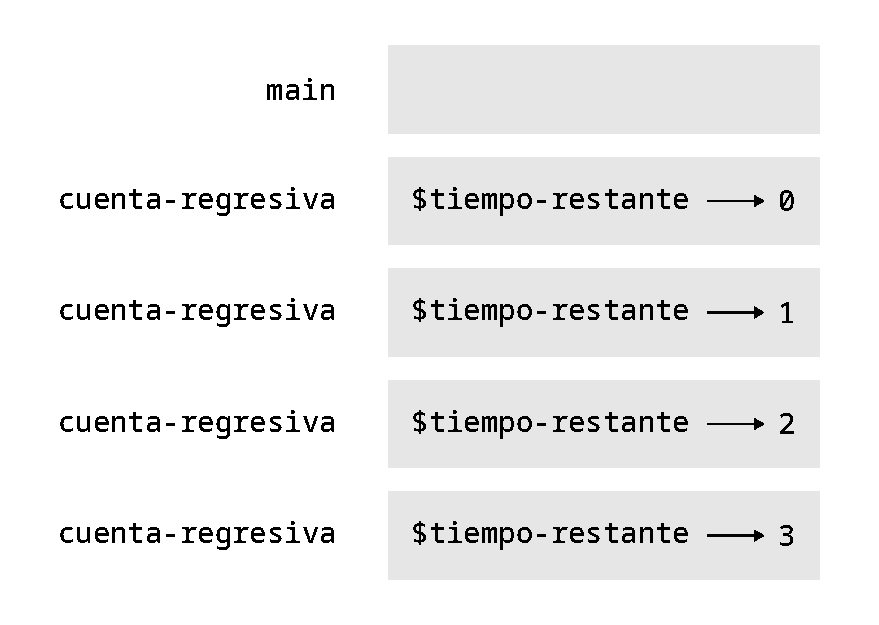
\includegraphics[scale=0.6]{figs/stack2.pdf}}
\caption{Stack diagram.}
\label{fig.stack2}
\end{figure}


Como siempre, la parte superior de la pila es el marco de
del programa principal.

Está vacío porque no creamos ninguna variable dentro del marco.
Tampoco pasamos ningún argumento al marco.
\index{base case}
\index{recursion!base case}

Los cuatro marcos de {\tt cuenta-regresiva} tienen diferente valores
para el parámetro {\tt \$tiempo-restante}. La parte inferior de la 
pila, donde {\tt \$tiempo-restante = 0}, se conoce como el {\bf caso base}.
El caso base no realiza una llamada recursiva y por lo tanto, no hay más
cuadros.

Como ejercicio, dibuja un diagrama de pila para la subrutina \verb|imprime-n-veces|
la cual se llama con los argumentos \verb|$sentence| y {\tt \$n = 2}.
Después escribe una función llamada \verb|hazlo-n-veces| que toma una función
y un número, {\tt \$num}, como argumentos, y llama la función 
provista {\tt \$num} veces.
\label{do_n_times}

Solución: ve la Sección~\ref{sol_do_n_times}


\section{Recursión Infinita}
\index{infinite recursion}
\index{recursion!infinite}
\index{runtime error}


Si una recursión nunca alcanza un caso base, se mantiene 
haciendo llamadas recursivas, y el programa nunca termina. Esto
se conoce como {\bf recursión infinita}, y generalmente no es 
una buena idea. De hecho, tu programa no se ejecutará por siempre
sino que terminará en algún punto cuando la computara agote la 
memoria disponible o algún otro recurso crítico.

Tienes que ser cuidadoso al escribir subrutinas recursivas. 
Asegúrate de tener un caso base, y comprueba que el programa
lo alcanzará. Actualmente, aunque esto no absolutamente requerido
por el lenguaje, te aconsejo que crees el hábito de tratar 
el caso base primero.

\section{Entrada del Teclado}
\index{keyboard input}

Los programas que hemos escrito hasta ahora no aceptan la
entrada de texto por el usuario. Ellos hace la mismas cosas
una y otra vez. Perl provee funciones integradas para parar
el programa y esperar que el usuario escriba algo.

Por ejemplo, la función {\tt prompt} incita al usuario a escribir
algo a través de una pregunta o una instrucción. Cuando el usuario 
presiona {\sf Return} o {\sf Enter}, el programa resume y 
la función \verb|prompt| devuelve lo que el usuario escribió 
como una cadena de texto (sin el carácter de nueva línea que 
corresponde a la tecla {\sf Return} que el usuario pulsa):
\index{prompt function}
\index{function!prompt}

\begin{lstlisting}
my $usuario = prompt "Por favor escribe tu nombre: ";
say "Hola $usuario";
\end{lstlisting}
%

Esta es probablemente una de las maneras más común de
obtener entrada interactiva de texto por el usuario, porque
es una buena idea dejarle saber lo que se espera.

Otra posibilidad es usar el método {\tt get} (el cual lee
una sola línea) en la entrada estándar:
\index{get function}
\index{function!get}

\begin{lstlisting}
say "Por favor escribe tu nombre: ";
my $usuario = $*IN.get;
say "Hola $usuario";
\end{lstlisting}
%
o la función {\tt get}, la cual lee una línea de la entrada
estándar por defecto:
\begin{lstlisting}
say "Por favor escribe tu nombre: ";
my $usuario = get;
say "Hola $usuario";
\end{lstlisting}
%

\section{Argumentos del Programa y la Subrutina MAIN}
\label{MAIN}
\index{MAIN}

Hay otra forma (y usualmente mejor) de hacer que un programa
use entrada variada definida por el usuario, lo cual es 
pasar argumentos desde la línea de comando al programa, de 
la misma manera en la que pasamos argumentos a nuestras subrutinas.

La manera más fácil de extraer argumentos que han sido pasados
al programa es con el uso de la subrutina especial \verb|MAIN|.
Un programa que tiene una subrutina \verb|MAIN| definida
comenzará usualmente su ejecución con esa subrutina, y los argumentos
de la línea de comando suministrados al programa serán pasados
como argumentos a \verb|MAIN|. La signatura \verb|MAIN| te 
permitará extraer los argumentos suministrados en la línea de comando
y posiblemente chequear la validad de los argumentos. 
\index{signature}

Por ejemplo, el programa {\tt saludar.pl6} podría lucir
así:
\begin{lstlisting}
sub MAIN (Str $nombre) {
    say "Hola $nombre";
}
\end{lstlisting}

Puedes llamar este programa dos veces con diferentes argumentos
en la línea de comando de tal forma:

\begin{lstlisting}
$ perl6 saludar.pl6 Larry
Hola Larry

$ perl6 greet.pl6 world
Hola world
\end{lstlisting}

Es muy fácil cambiar el argumento, debido a que todo lo que
necesitas hacer en la línea de comando del sistema operativo
es usar la flecha y editar el final de la línea de comando
anterior.

Si olvidas suministrar un argumento (o provees el número 
equivocado de argumentos, o los argumentos no coinciden con
la signatura), el programa terminará y Perl~6 generará
y mostrará el modo de uso:

\begin{lstlisting}
$ perl6 saludar.pl6
Usage:
  saludar.pl6 <nombre>
\end{lstlisting}


\section{Depuración de programas}
\label{whitespace}
\index{debugging}
\index{traceback}

Cuando ocurre un error de sintaxis o un error al tiempo de ejecución,
el mensaje de error contiene mucha información, aunque puede ser
agobiante. Las preguntas más útiles son usualmente:

\begin{itemize}

\item ?`Qué tipo de error fue?

\item ?`Dónde ocurrió?

\end{itemize}

Los errores sintácticos son usualmente fáciles de encontrar,
sin embargos existen algunos trucos. En general, los mensajes 
de error indican donde se descubrió el problema, aunque el actual
error podría encontrarse un poco antes, algunas veces en la 
línea previa o hasta varias líneas antes.
\index{multiplication tables}

Por ejemplo, el objetivo del siguiente código era mostrar
la tabla de multiplicación:

\begin{lstlisting}
# ADVERTENCIA: código con fallas
sub tabla-multiplicación {
    for 1..10 -> $x {
        for 1..10 -> $y {
            say "$x x $y\t= ", $x * $y;
        say "";
    }
}

tabla-multiplicación();
\end{lstlisting}

Falló al tiempo de compilación con el siguiente error:

\begin{lstlisting}
$ perl6 tabla_mult.pl6
===SORRY!=== Error while compiling /home/Laurent/tabla_mult.pl6
Missing block (taken by some undeclared routine?)
at /home/Laurent/tabla_mult.pl6:9
------> tabla-multiplicación();<HERE><EOL>
\end{lstlisting}

El mensaje de error reporta un error en la línea~9 del 
programa (la última línea del código), al final de la línea,
pero el error actual es que falta una llave izquierda después
de la línea~4 y antes de la línea~5. La razón de esto es que,
mientras el programador cometió el error en la línea~4,
el interpretador de Perl no pudo detectar este error antes 
de alcanzar el final del programa. El programa correcto para mostrar
la table de multiplicación podría ser:

\begin{lstlisting}
sub tabla-multiplicación {
    for 1..10 -> $x {
        for 1..10 -> $y {
            say "$x x $y\t= ", $x * $y;
        }
        say "";
    }
}
tabla-multiplicación();
\end{lstlisting}

Cuando un error es reportado en la última línea de un
programa, es comúnmente causado por la falta de un
paréntesis, un corchete, una llave, o una comilla varias
líneas más arriba. Un editor con coloración de sintaxis
puede algunas veces ayudarte a resolver este error.
\index{syntax!highlighting}

\index{error!runtime}
\index{runtime error}

Lo mismo sucede con errores al tiempo de ejecución. Considera
este programa cuyo objetivo es calcular 360 grados divididos
sucesivamente por los enteros entre 2 y 5:

\begin{lstlisting}
# ADVERTENCIA: código con fallas
my ($a, $b, $c, $d) = 2, 3, 5;
my $valor = 360;
$valor /= $_ for $a, $b, $c, $d;
say $valor;
\end{lstlisting}

Esto programa compila correctamente pero muestra una
advertencia y después una excepción al tiempo de ejecución:

\begin{lstlisting}
Use of uninitialized value of type Any in numeric context 
in block  at producto.pl6 line 3
Attempt to divide 12 by zero using div
  in block <unit> at producto.pl6 line 4
\end{lstlisting}
%

El mensaje de error indica una excepción ``division by zero''
en la línea~4, pero no hay nada
incorrecto con esa línea. La advertencia en la línea~3
podría darnos una pista sobre el intento del script 
de usar un valor indefinido, pero el error real se encuentra 
en la primera línea del script, donde uno de los cuatros 
enteros necesarios fue omitido por equivocación en la
asignación de la lista.

\index{division by zero}
\index{uninitialized value}

Deberías prestarle atención a los mensajes de error y leerlos
cuidadosamente. Sin embargo, no asumas que ellos apuntan a la
causa de la excepción; usualmente ellos apuntan 
a problemas subsecuentes.


\section{Glosario}

\begin{description}

\item[División de enteros] Una operación, denotada por {\tt div},
que divide dos números y redondea el resultado.
  \index{integer division} 
  \index{division!integer}

\item[Operador de módulo]  Un operador, denotado por un signo
de porcentaje ({\tt \%}), que funciona con números enteros y devuelve
el residuo al dividir un número por otro.
\index{modulo operator}
\index{operator!modulo}

\item[Expresión Booleana]  Una expresión cuyo valor es 
{\tt True} o {\tt False}.
\index{Boolean expression}
\index{expression!Boolean}

\item[Operador de relación] Uno de los operadores que compara
sus operandos. Los operadores de relación numérica más comunes son 
{\tt ==}, {\tt !=}, {\tt >}, {\tt <}, {\tt >=}, y {\tt <=}. 
Los operadores equivalentes de relación de cadenas de texto 
son {\tt eq}, {\tt ne}, {\tt gt}, {\tt lt}, {\tt ge}, and {\tt le}.

\item[Operador lógico] Uno de los operadores que combina expresiones
Booleanas: {\tt and}, {\tt or}, y {\tt not}. Los 
operadores equivalentes de precedencia superior son
{\tt \&\&}, {\tt ||}, y {\tt !}

\item[Sentencia condicional]  Una sentencia que controla el flujo
de ejecución dependiendo en algunas condiciones.
\index{conditional!statement}
\index{statement!conditional}

\item[Condición] La expresión booleana en una sentencia
condicional que determina cual de las ramas se ejecuta.
\index{condition}

\item[Rama] Una de las secuencias alternativas de sentencias
en una sentencia condicional.
\index{branch}

\item[Condicional encadenada]  Una sentencia condicional con 
una serie de ramas alternativas.
\index{chained conditional}
\index{conditional!chained}

\item[Condicional anidada]  Una sentencia condicional que aparece
en una de las ramas de otra sentencia condicional.
\index{nested conditional}
\index{conditional!nested}

\item[Modificador de sentencia] Una expresión condicional sufija,
i.e., una expresión condicional (usando por ejemplo {\tt if}, {\tt unless} o 
{\tt for}) que es colocada después de la sentencia cuya ejecución
controla. También puede referirse a una expresión de bucle sufijo.
\index{statement modifier}

\item[Sentencia de retorno] Una sentencia que forza a una 
función a terminar de inmediato y devolver a la función
que realiza la llamada.

\item[Recursión]  El proceso de llamar una función 
que aún está en ejecución.
\index{recursion}

\item[Caso base]  Una rama condicional en una función
recursiva que no realiza una llamada recursiva.
\index{base case}

\item[Recursión infinita]  Una recursión que carece
de un caso base, o que nunca lo alcanza. Eventualmente, 
una recursión infinita causa un error al tiempo de ejecución,
por el cual no querrás esperar dado que podría tardar demasiado.
\index{infinite recursion}

\end{description}

\section{Ejercicios}
%

\begin{exercise}
%
Usando los operadores división de enteros y módulo:
\index{modulo operator}
\index{operator!mod}
\index{mod, modulo operator}
\index{integer division}
\index{operator!div}
\index{div operator}
\label{int_div_modulo}

\begin{enumerate}

\item Escribe una subrutina que calcule cuantos días, horas, minutos y segundos
hay en el número de segundos pasado como argumento a la subrutina.

\item Escribe un script que calcule cuantos días, horas, minutos y segundos 
hay en 240, 000 segundos.

\item Cambia el script para calcular el número de días, horas, minutos y segundos
que hay en un número de segundos proveído por el usuario cuando se le
pide proveer un número de segundos.

\end{enumerate}

Soluciones: Subsección~\ref{sol_int_div_modulo}.

\end{exercise}


\begin{exercise}
\index{Fermat's Last Theorem}
\label{fermat_ex}

El último teorema de Fermat enuncia que no existen números enteros
positivos $a$, $b$, y $c$ tales que se cumpla:

\[ a^n + b^n = c^n \]
%
para todos los valores de $n$ mayores que 2.

\begin{enumerate}

\item Escribe una función con el nombre \verb|chequear-fermat| que
toma cuatro parámetros---{\tt a}, {\tt b}, {\tt c}, y {\tt n}---y
chequea si se cumple el teorema de Fermat. Si $n$ es mayor que 2 y 

\[a^n + b^n = c^n \]
%
el programa debería imprimir, ``!`Santo dios, Fermat estaba equivocado!``
Por lo contrario, el programa debería imprimir ``Ǹo, eso no funciona.``

\item Escribe una subrutina que incita al usuario a entrar valores para 
las variables {\tt a}, {\tt b}, {\tt c}, y {\tt n}, los convierte a enteros,
y usa la función \verb|chequear-fermat| para chequear si ellos violan
el teorema de Fermat.
\end{enumerate}

Solución: \ref{sol_fermat_ex}


\end{exercise}


\begin{exercise}
\index{triangle}
\label{triangle}

Si se te provee con tres palillos, podrías o no podrías 
ser capaz de organizarlos en un triángulo.
Por ejemplo, si uno de los palillos tiene una longitud de 
12 pulgadas y los restantes tienen 1 pulgada, no podrás
conseguir que los palillos pequeños se encuentren en 
el medio. Para tres longitudes cualquiera, existe una 
simple prueba para ver si es posible crear un triángulo:

\begin{quotation}
Si una de las tres longitudes es mayor que la suma de las
otras dos, entonces no puedes formar una triángulo. De lo
contrario, puedes formar un triángulo. (Si la suma de dos
lados es igual al tercero, ellos forman lo que se
conoce como un triángulo "degenerado".)
\end{quotation}

\begin{enumerate}

\item Escribe una función llamada \verb|es-triángulo| que toma
tres números positivos como argumentos, e imprime ``Sí`` o ``No,``
dependiendo si puedes formar un triángulo con las longitudes
dadas.

\item Escribe una función que incite al usuario a entrar
tres longitudes y use la función \verb|es-triángulo| para 
chequear si palillos con las longitudes dadas pueden formar 
un triángulo.
\end{enumerate}

Solución: \ref{sol_triangle}


\end{exercise}

\begin{exercise} 
\index{Fibonacci!numbers}
\label{fibonacci}
Los números Fibonacci fueron inventados por Leonardo Fibonacci 
(también conocido como Leonardo de Pisa o simplemente, Fibonacci), 
un matemático italiano del siglo XIII.
\index{Fibonacci, Leonardo}

Los números Fibonacci son una secuencia de números como tal:

\[1, \;1, \;2, \;3, \;5, \;8, \;13, \;21, \;34, \ldots\]
%
en la cual los primeros dos números son 1 y cada número 
subsecuente de la secuencia está definido como la suma de
los dos números anteriores (por ejemplo, $5 = 2 + 3$, $8 = 3 + 5$, etc.).

En notación matemática, los números Fibonacci 
podrían ser definidos por una relación de recurrencia  
de la siguiente manera:

\[F_1 = 1, \;F_2 = 1, \;\;and\;\;  F_n = F_{n-1} + F_{n-2} \]
%
\begin{enumerate}

\item  Escribe un programa usando el bucle {\t for} que imprime
en la pantalla los primeros 20 números Fibonacci.

\item Escribe un programa que incite al usuario a entrar un número $n$ y,
usando el bucle {\tt for}, calcule y muestre el número Fibonacci $n^{th}$.
\end{enumerate}

Solución: \ref{sol_fibonacci}


\end{exercise}

\begin{exercise}
\label{sub_recurse}
\index{recursion}

?`Cuál es la salida del siguiente programa?
Dibuja un diagrama de pila que muestre el estado del 
programa cuando imprime el resultado.

\begin{lstlisting}
sub recurse($n, $s) {
    if ($n == 0) {
        say $s;
    } else {
        recurse $n - 1, $n + $s;
    }
}
recurse 3, 0;
\end{lstlisting}

\begin{enumerate}

\item ?`Qué pasaría si llamaras la función de la siguiente forma:
{\tt recurse(-1, 0)}?

\item Escribe un comentario de documentación (quizás en la forma de un comentario multilínea) que explique todo lo que alguien necesita saber para usar esta función (y nada más).
\end{enumerate}

Solución: \ref{sol_sub_recurse}

\end{exercise}





\chapter{Subrutinas Fructuosas}
\label{fruitchap}

La mayoría de funciones de Perl que hemos usado, tales como
la funciones matemáticas, producen valores de retorno. Aún así,
la mayoría de funciones que hemos escrito hasta ahora son funciones
void: ellas tienen un efecto, como imprimir un valor,
pero no tienen un valor de retorno. En este capítulo, aprenderás
a escribir funciones fructuosas.

\section{Valores de Retorno}
\index{return!value}

Al llamar una función fructuosa de genera un valor de retorno,
el cual usualmente asignamos a una variable o usamos como 
parte de una expresión:

\begin{lstlisting}
my $pi = 4 * atan 1;
my $altura = $radio * sin $radianes;
\end{lstlisting}
%
Muchas de las subrutinas que hemos escrito hasta ahora son
void. Hablando casualmente, ellas no tienen un valor de 
retorno útil; más precisamente, su valor de retorno puede
ser {\tt Any}, {\tt Nil}, {\tt ()}, o {\tt True}.

En este capítulo, finalmente escribiremos subrutinas fructuosas. 
El primer ejemplo es {\tt area}, la cual devuelve el área de un 
círculo con un radio en particular:

\begin{lstlisting}
sub area($radio) {
    my $area_circular = pi * $radio**2;
    return $area_circular;
}
\end{lstlisting}
%
Hemos visto la sentencia {\tt return} anteriormente,
pero en una subrutina fructuosa la sentencia {\tt return} 
incluye una expresión. Esta sentencia quiere decir: ``
Devuelve inmediatamente desde esta función y usa la siguiente
expresión como un valor de retorno.``
La expresión puede ser arbitrariamente complicada, así podríamos
esta función en una manera más concisa:
\index{return!statement}
\index{statement!return}

\begin{lstlisting}
sub area($radio) {
    return pi * $radio**2;
}
\end{lstlisting}
%

Por otro lado, las {\bf variables temporales} 
como \verb|area_circular| hace la depuración mucho más
fácil. También ayudar a documentar lo que está sucediendo
en la función.
\index{temporary variable}
\index{variable!temporary}

Algunas veces es útil tener varias sentencias return, por 
ejemplo una en cada rama de una condicional:

\begin{lstlisting}
sub valor_absoluto($num){
    if $num < 0 {
        return -$num;
    } else {
        return $num;
    }
}
\end{lstlisting}
%
Dado que estas sentencias {\tt return} están en una 
condicional alternativa, solo una se ejecuta.

Esto podría también escribirse de forma concisa usando sintaxis 
del modificador de sentencia:

\begin{lstlisting}
sub valor_absoluto($num){
    return -$num if $num < 0;
    return $num;
}
\end{lstlisting}
%
Otra vez, solo una de las sentencias return se ejecuta: si el 
número es negativo, la primera sentencia return es ejecutada
y la ejecución de la subrutina termina ahí; en cambio, si el
número es positivo o cero, solo la segunda sentencia return 
es ejecutada.

Tan pronto una sentencia return es ejecutada, la función termina
sin ejecutar las sentencias subsecuentes. Cualquier código que aparece
después de una sentencia {\tt return} incondicional, o cualquier
otro lugar que el flujo de ejecución no puede alcanzar es 
conocido como {\bf código muerto}. 
\index{dead code}

En una función fructuosa, es buena idea asegurar que cada
posible ruta a través del programa alcance con una sentencia
{\tt return}. Por ejemplo:

\begin{lstlisting}
# ADVERTENCIA: código con fallas
sub valor_absoluto($num){
    if $num < 0 {
        return -$num;
    } 
    if $num > 0 {
        return $num;
    }
}
\end{lstlisting}
%

Esta subrutina es incorrecta porque si {\tt \$num} es 0, 
ninguna de las condiciones es verdadera, y la subrutina termina 
sin alcanzar una sentencia {\tt return}. Si el flujo de ejecución
llega al final de una función, el valor de retorno es {\tt ()}, que básicamente
significa ``no definido`` y claramente no es el valor absoluto de 0:
\index{undefined value}

\begin{lstlisting}
> valor_absoluto(0)
()
\end{lstlisting}
%
Casualmente, Perl provee una función integrada
llamada {\tt abs} que calcula valores absolutos.
\index{abs function or method}
\index{function!abs}

\label{compare}
Como ejercicio, escribe una subrutina {\tt comparar}
que toma dos números, {\tt \$x} y {\tt \$y}, y devuelve
{\tt 1} si {\tt \$x > \$y}, {\tt 0} if {\tt \$x == \$y}, y 
{\tt -1} if {\tt \$x < \$y}.

Solución: \ref{sol_compare}
\index{compare function}
\index{function!compare}


\section{Desarrollo Incremental}
\label{incremental.development}
\index{development plan!incremental}
\index{incremental development}

A medida que escribes funciones más largas, puedes 
pasar más tiempo depurando.

Para tratar con programas complejos, podrías querer 
usar un proceso llamado {\bf desarrollo incremental}. El 
objetivo del desarrollo incremental es evitar sesiones largas\
y tediosas de depuración al añadir y evaluar una pequeña pieza
de código a la vez.
\index{testing!incremental development}
\index{Pythagorean theorem}

Como un ejemplo, supón que quieres encontrar la distancia 
entre dos puntos, dadas las coordenadas cartesianas o rectangulares
$(x_1, y_1)$ y $(x_2, y_2)$ de los puntos. Por el teorema de Pitágoras,
la distancia es:
\index{Pythagorean theorem}
\index{Cartesian coordinates}
\index{coordinates!Cartesian}
\index{rectangular!coordinates}
\index{coordinates!rectangular}


\begin{displaymath}
\mathrm{distancia} = \sqrt{(x_2 - x_1)^2 + (y_2 - y_1)^2}
\end{displaymath}
%
El primer paso es considerar cómo la función {\\t distancia} 
debería lucir en Perl. En otras palabra,cuáles son las entradas (parámetros)
y cuál es la salida (valor de retorno)?

En este caso, las entradas son los puntos, los cuales puedes 
representar usando cuatros números. El valor de retorno es la distancia
representada por un valor numérico.

Inmediatamente puedes escribir un bosquejo de la función:

\begin{lstlisting}
sub distancia($x1, $y1, $x2, $y2) {
    return 0.0;
}
\end{lstlisting}
%
Obviamente, esta versión no calcula la distancia; siempre 
devuelve cero. Sin embargo, es sintácticamente correcta, y 
puede ser ejecutada, lo que significa que la probaste antes 
de hacerla más complicada.

Para probar la nueva función, llámala con algunos argumentos:

\begin{lstlisting}
> distancia(1, 2, 4, 6);
0.0
\end{lstlisting}
%
Elegí estos valores para que la distancia horizontal sea 3 y la distancia
vertical seaa 4; de esa manera, el resultado es 5, la hipotenusa de 
un triángulo 3-4-5. Al probar una función, es siempre útil saber la 
respuesta correcta.
\index{testing!knowing the answer}

En este momento, hemos confirmado que la función es sintácticamente 
correcta, y podemos comenzar a añadir código al cuerpo de
la función. Un siguiente paso razonable es encontrar las diferencias
$x_2 - x_1$ and $y_2 - y_1$.  La siguiente versión almacena esos valores
en variable temporales y los imprime:

\begin{lstlisting}
sub distancia($x1, $y1, $x2, $y2) {
    my $dx = $x2 - $x1;
    my $dy = $y2 - $y1;
    say '$dx es', $dx;
    say '$dy es', $dy;
    return 0.0;
}
\end{lstlisting}
%
Si la subrutina funciona como debe, debería mostrar \verb"$dx es 3" y 
\verb"$dy es 4" (y todavía devolver 0.0). Si esto sucede, sabemos
que la función está recibiendo los argumentos correctos y realizando
la primera computación correctamente. Por lo contrario, si esto no sucede
solo tenemos que depurar algunas líneas.

El siguiente paso es computar la suma de los cuadrados de {\tt \$dx} y 
{\tt \$dy}:

\begin{lstlisting}
sub distancia($x1, $y1, $x2, $y2) {
    my $dx = $x2 - $x1;
    my $dy = $y2 - $y1;
    my $dist-cuadrada = $dx**2 + $dy**2;
    say '$dist-cuadrada es: ', $dist-cuadrada;
    return 0.0;
}
\end{lstlisting}
%
Otra vez, ejecutarías el programa en esta etapa y 
chequearías la salida (que debería ser 25).
Finalmente, puedes usar la función integrada {\tt sqrt} 
para calcular la raíz cuadrada y devolver el resultado:
\index{sqrt function}
\index{function!sqrt}

\begin{lstlisting}
sub distancia($x1, $y1, $x2, $y2) {
    my $dx = $x2 - $x1;
    my $dy = $y2 - $y1;
    my $dist-cuadrada = $dx**2 + $dy**2;
    my $resultado = sqrt $dist-cuadrada;
    return $resultado;
}
\end{lstlisting}
%
Si eso funciona correctamente, ya acabaste. Por lo contrario,
podrías imprimir el valor de {\tt \$resultado} antes de la
sentencia return.

La versión final de la subrutina no muestra nada cuando se ejecuta;
solo devuelve un valor. Las sentencias {\tt print} que escribimos
son útiles para la depuración, pero una vez que consigues que la subrutina
funcione correctamente, puedes removerlas. Código como ese es algunas
veces llamado {\tt andamiaje} porque es útil para construir el programa
pero no forma parte del producto final.
\index{scaffolding}

Cuando empiezas a programar, debes agregar una o dos líneas de código
al mismo tiempo. A medida que ganas experiencia, puedes entonces escribir
y depurar piezas más grandes. De cualquier manera, el desarrollo incremental
puede salvarte muchas horas de depuración.

Los aspectos claves del proceso son:
\begin{enumerate}

\item Comienza con un programa que funcione y haz pequeños cambios
incrementales. En cualquier punto, si hay un error, deberías entonces
tener una buena idea donde se encuentra.

\item Usa variables para almacenar los valores intermedios
para que puedas mostrarlos y chequearlos

\item Una vez que el programa funciona, podrías querer remover
algo del código de andamiaje o consolidar sentencia múltiples
en una expresión compuesta, pero solo si no dificulta la lectura
del programa.

\end{enumerate}

Nota que, por lo menos para casos relativamente simples, 
puedes usar el REPL para probar expresiones y hasta sentencias
multilíneas o subrutinas en el modo interactivo antes de 
incluirlas en tu código. Esto es usualmente rápido y puede 
ahorrarte algún tiempo.
\index{REPL}
\index{interactive mode}

\label{hypotenuse}
Como ejercicio, usa el desarrollo incremental para escribir
una función llamada {\tt hipotenusa} que devuelve la longitud de
la hipotenusa de un triángulo rectángulo, dadas las longitudes de
los otros dos lados como argumentos. Registra cada etapa del
desarrollo a medida que avanzas.

Solución: \ref{sol_hypotenuse}.
\index{hypotenuse}



\section{Composición}
\index{composition}
\index{function composition}

Como deberías saber por ahora, tú puedes llamar una función
desde otra. Como un ejemplo, escribiremos una función 
que toma dos puntos, el centro del círculo y un punto en el 
perímetro, y calcula el área del círculo.

Asume que el centro es almacenado en las variables {\tt \$x-c} y
{\tt \$y-c}, y el perímetro está en {\tt \$x-p} y {\tt \$y-p}. 
El primer paso es encontrar el radio del círculo, el cual es la 
distancia entre los dos puntos. Anteriormente escribimos una función,
{\tt distancia}, que hace exactamente eso:

\begin{lstlisting}
my $radio = distancia($x-c, $y-c, $x-p, $y-p);
\end{lstlisting}
%
El siguiente paso es encontrar el área de un círculo 
con ese radio; también escribimos algo para hacer eso mismo:

\begin{lstlisting}
my $resultado = area($radio);
\end{lstlisting}
%
Al encapsular estos pasos en una función, tenemos:
\index{encapsulation}

\begin{lstlisting}
sub area-círculo($x-c, $y-c, $x-p, $y-p) {
    my $radio = distancia($x-c, $y-c, $x-p, $y-p);
    my $resultado = area($radio)
    return $resultado;
}
\end{lstlisting}
%
Las variables temporarias {\tt \$radio} y {\tt \$resultado} son útiles
para el desarrollo y la depuración, pero una vez que el programa ya funciona
adecuadamente, podemos hacer todo más conciso al componer las llamadas
de las funciones:

\begin{lstlisting}
sub area-círculo($x-c, $y-c, $x-p, $y-p) {
    return area distancia($x-c, $y-c, $x-p, $y-p);
}
\end{lstlisting}
%

La última línea del ejemplo anterior ahora funciona como
un conducto (del inglés \emph{pipeline}) de datos desde la 
derecha hacia la izquierda; la función \verb|distancia| toma 
los cuatros argumentos y devuelve una distancia (el radio)
el cual se pasa como una argumento a \verb|area|; con este
argumento, \verb|area| es ahora capaz de devolver el área,
la cual es entonces devuelta por \verb|area-círculo| al
código que hace la llamada. Regresaremos más tarde a este modelo
de conducto de datos.
\index{pipe-line programming}

\section{Funciones Booleanas}
\label{boolean}

Las funciones pueden devolver valores Booleanos, lo cual es usualmente
conveniente para ocultar pruebas complicadas dentro de las funciones. Por
ejemplo:
\index{Boolean function} 

\begin{lstlisting}
sub es-divisible(Int $x, Int $y) {
    if $x % $y == 0 {
        return True;
    } else {
        return False;
    }
}
\end{lstlisting}
%
Es común darle a las funciones Booleanas nombres que suenan como
preguntas con respuestas de sí/no; \verb|es-divisible|, por ejemplo,
devuelve {\tt True} o {\tt False} para indicar si {\tt x} es divisible
por {\tt y}.

Este es un ejemplo:

\begin{lstlisting}
> es-divisible(6, 4);
False
> es-divisible(6, 3);
True
\end{lstlisting}
%
El resultado del operador {\tt ==} es un valor Booleano,
así que podemos escribir la subrutina de manera concisa al 
devolverlo directamente:

\begin{lstlisting}
sub es-divisible(Int $x, Int $y) {
    return $x % $y == 0
}
\end{lstlisting}
%
Si no hay una sentencia de retorno, una subrutina en Perl devuelve
el valor de la expresión en la última línea de código de la 
subrutina (provisto que la última expresión sea una expresión
que puede ser evaluada), así que la sentencia {\tt return} no 
es requerida aquí. Además, dado que 0 es una valor falso y cualquier 
otro entero es un valor verdadero, la misma subrutina podría escribirse
de otra forma:

\begin{lstlisting}
sub es-divisible(Int $x, Int $y) { 
    not $x % $y 
}
\end{lstlisting}

Las declaraciones de tipo {\tt Int} en las signaturas de la subrutina
más arriba no son necesarias. La subrutina funcionaría sin ellas, pero
ellas pueden proveer algún tipo de protección en contra del uso 
de esta subrutina con argumentos defectuosos.

Las funciones Booleanas se usan usualmente en los 
modificadores de sentencias:
\index{statement modifier}
\index{modifier!statement}

\begin{lstlisting}
say "$x es divisible por $y" if es-divisible($x, $y);
\end{lstlisting}
%
Podría ser tentativo escribir algo como:

\begin{lstlisting}
say "$x es divisible por $y" if es-divisible($x, $y) == True;
\end{lstlisting}
%
Pero la comparación extra no es necesaria: 
{\tt es-divisible} devuelve un valor Booleano que puede ser
interpretado directamente por la condicional {\tt if}.

\label{isbetween}
Como ejercicio, escribe una función \verb|está-entre(x, y, z)|
que devuelve {\tt True} si $x \le y \le z$ o por lo contrario,
{\tt False}.

Solución: \ref{sol_isbetween}.

\section{Un Lenguaje de Programación Completo}

En la sección anterior vimos varias maneras de escribir
una subrutina para chequear la divisibilidad de dos 
enteros.
\index{divisibility}

De hecho, como fue mencionado anteriormente, Perl~6
tiene un operador ``es-divisible``, \verb|%%|, el cual
devuelve {\tt True} si el número en la izquierda es divisible
por el de la derecha:
%\index{%%!is divisible operator}
\index{is divisible operator}

\begin{lstlisting}
> 9 %% 3
True
> 9 %% 4
False
\end{lstlisting}

Por lo tanto no había necesidad de escribir la subrutina
{\tt es-divisible}. Pero no te preocupes, es totalmente 
normal si no recordaste eso. A los hablantes de lenguajes 
naturales se les permite tener diferentes niveles de cualificación,
aprender a medida que avanzan, y poner el lenguaje a buen uso 
antes de que sepan el lenguaje completo. Lo mismo pasa con Perl.
Tú (y yo) no sabemos todo sobre Perl~6 todavía, al igual que no
sabemos todo sobre el inglés (o el español). Pero es de hecho 
``Oficialmente Okay en la Cultura de Perl`` usar el subconjunto
del lenguaje que sabes. De hecho, se fomenta a que uses lo que es
a veces llamado ``baby Perl`` para escribir programas, aunque sean
un poco toscos y rudimentarios al principio. Esa es la mejor manera 
de aprender Perl, del mismo que ``hablar como un bebé`` (``baby talk``) es
la mejor manera para que un niño aprenda inglés (o español).
\index{baby Perl}
\index{Perl culture}

El número de maneras diferentes de llevar a cabo una tarea,
tal como chequear si un número es divisible por otro,
es un ejemplo del lema de Perl:
\emph{there is more than one way to do it 
(Hay más de una forma para hacer algo)}, usualmente abreviado TIMTOWTDI.
Algunas maneras pueden ser más concisa o más eficiente que
otras, pero, en la filosofía de Perl, tú estás perfectamente 
facultado para hacerlo a tu manera, especialmente si eres
un principiante, provisto que encuentres el resultado 
correcto.
\index{there is more than one way to do it}
\index{TIMTOWTDI}
\index{Turing!complete language}
\index{language!Turing complete}
\index{Turing, Alan}
\index{Turing!thesis}

Hasta ahora, solamente hemos cubierto un pequeño subconjunto de Perl~6,
pero te sería interesante saber que este subconjunto es un lenguaje
de programación \emph{completo}, lo cual significa que esencialmente
cualquier cosa que puede computarse podría expresarse en este 
lenguaje. Cualquier programa que se haya escrito jamás podría escribirse
de nuevo solo usando las características del lenguaje que has aprendido
hasta ahora (actualmente, solo necesitarías algunos comandos para
controlar dispositivos como el ratón, discos, redes, etc., pero eso 
es todo).

La prueba de esa afirmación no es un ejercicio trivio. El primero
en probarla fue Alan Turing, uno de los primeros científicos de la
computación (algunas personas argumentan que él fue un matemático, sin 
embargo muchos de los primeros científicos de la computación comenzaron 
como matemáticos). Por esta razón, se le conoce como la prueba de Turing
(\emph{Turing Test}). Para una discusión más completa (y precisa) de la
prueba de Turing, recomiendo el libro  {\em Introduction to the
Theory of Computation} de Michael Sipser.

\section{Más Recursión}
\label{more.recursion}
\index{recursion}


Para darte una idea de lo que puedes hacer con las herramientas
que has aprendido hasta ahora, evaluaremos algunas funciones 
matemáticas definidas de forma recursiva. Una definición recursiva
es similar a una definición circular, en el sentido de que la 
definición contiene una referencia a la cosa que se define. 
Una definición verdaderamente circular no es muy útil:

\begin{description}

\item[Vorpal] An adjective used to describe something that is vorpal.
\index{vorpal}
\index{circular definition}
\index{definition!circular}

\end{description}

Si ves esa definición en el diccionario, podrías enojarte. 
Sin embargo, si busca la definición de la función factorial,
denotada con el símbolo $!$, podrías conseguir algo como esto:
%
\begin{eqnarray*}
&&  0! = 1 \\
&&  n! = n (n-1)!
\end{eqnarray*}
%
Esta definición dice que el factorial de 0 es 1, y que el factorial
de cualquier otro valor (entero positivo), $n$, es 
$n$ multiplicado por el factorial de $n-1$.

Así que $3!$ es 3 por $2!$, el cual es 2 por $1!$, el cual es 1 por
$0!$. Si lo ponemos todo junto, $3!$ es igual a 3 por 2 por 1 por 1, 
lo cual es 6.
\index{factorial!function}
\index{function!factorial}
\index{recursive definition}

Si puedes escribir una definición recursiva de algo, puedes escribir
un programa de Perl para evaluar dicha definición. El primer paso
es decidir cuáles deberían ser los parámetros. En este caso, es
claro que el factorial toma un número\footnote{Debería ser realmente un entero, pero regresaremos a esto más tarde en este capítulo.}:

\begin{lstlisting}
sub factorial($n){
}
\end{lstlisting}
%
Si el argumento es 0, todo lo que tenemos que hacer es devolver es 1:

\begin{lstlisting}
sub factorial($n){
    if $n == 0 {
        return 1;
    }
}   
\end{lstlisting}
%
Por el otro lado, y ésta es la parte interesante, tenemos que hacer
una llamada recursiva para encontrar el factorial de $n-1$ y después
multiplicarlo por $n$:
\index{factorial!using recursion}

\begin{lstlisting}
sub factorial($n){
    if $n == 0 {
        return 1;
    } else {
        my $recurse = factorial($n-1);
        my $result = $n * $recurse;
        return $result;
    }
}
\end{lstlisting}
%
El flujo de ejecución para este programa es similar al flujo de 
{\tt cuenta-regresiva} en la Sección~\ref{recursion}. Si llamamos
a {\tt factorial} con el valor 3:

Dado que 3 no es 0, tomamos la segunda rama y calculamos el factorial de
{\tt \$n-1}...

\begin{quote}
Dado que 2 no es 0, tomamos la segunda rama y calculamos el factorial de
{\tt \$n-1}...


  \begin{quote}
  Dado que 1 no es 0, tomamos la segunda rama y calculamos el factorial de
  {\tt \$n-1}...


    \begin{quote}
    Dado que 0 es igual a 0, tomamos la primera rama y devolvemos 1
    sin hacer más llamadas recursivas.
    \end{quote}

	
  El valor de retorno, 1, es multiplicado por \verb|$n|, el cual es 1,
  y se devuelve el resultado.
  \end{quote}


El valor de retorno, 1, es multiplicado por \verb|$n|, el cual es 1,
y se devuelve el resultado.
\end{quote}


El valor de retorno, 2, es multiplicado por \verb|$n|, el cual es 3,
el resultado, 6, se convierte en el valor de retorno de la llamada
de subrutina que inició todo el proceso.
\index{stack diagram}

La figura~\ref{fig.stack3} muestra como el diagrama de pila luce para esta
secuencia de llamadas de función.

\begin{figure}
\centerline
{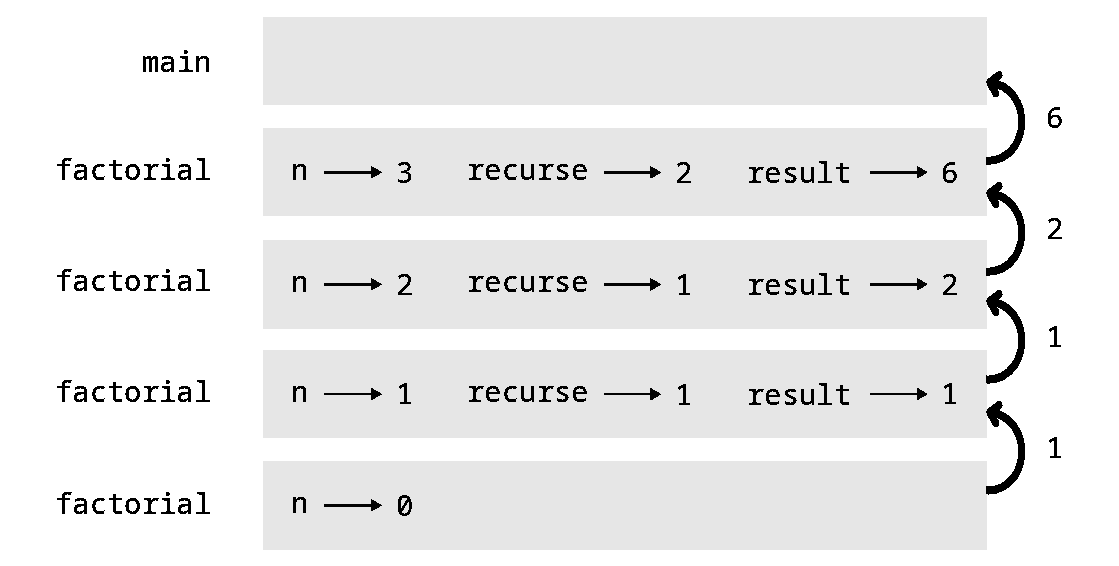
\includegraphics[scale=0.7]{figs/stack3.pdf}}
\caption{Diagrama de pila.}
\label{fig.stack3}
\end{figure}

Los valores de retorno se muestran siendo pasados devuelta a la pila. En cada
cuadro, el valor de retorno es el valor de {\tt result}, el cual es 
producto de {\tt n} y {\tt recurse}.
\index{function!frame}
\index{frame}

En el último cuadro, las variables locales {\tt recurse} y {\tt result}
no existen, porque la rama que las crea no se ejecuta.

Un programador de Perl con experiencia podría escribir una
subrutina más concisa o más idiomática\footnote{Luego veremos 
más formas idiomáticas de computar el factorial de un número.}:
\index{idiomatic}

\begin{lstlisting}
sub factorial($n){
    return 1 if $n == 0;
    return $n * factorial $n-1;
}
\end{lstlisting}
%
Esto es no mejor que nuestra primera versión, y probablemente
no se ejecutará significativamente más rápido, pero es presumiblemente
más clara, por lo menos cuando te acostumbra a este tipo de sintaxis.

\section{Acto de Fe}
\index{recursion}
\index{leap of faith}

Seguir el flujo de ejecución es una manera de leer un programa,
pero se vuelve agobiante en poco tiempo. Una alternativa es 
lo que puede ser llamada el ``acto de fe``. Cuando encuentras 
una subrutina, en lugar de seguir el flujo de ejecución,
tu \emph{asumes} que la subrutina funcione correctamente y devuelve
el resultado correcto.


De hecho, estás ya practicando este acto de fe cuando usas las funciones
integradas. Cuando llamas las funciones matemáticas tales como {\tt cos} 
o {\tt sqrt}, no examinas los cuerpos de esas funciones. Asumes que funcionan
adecuadamente porque las personas que escribieron las funciones 
integradas eran probablemente buenos programadores (y porque puedes
asumir seguramente que dichas funciones han sido probadas extensivamente).

Lo mismo es cierto cuando llamas una de tus subrutinas. Por ejemplo,
en la Sección~\ref{boolean}, escribimos una subrutina llamada \verb|es-divisible|
que determina si un número es divisible por otro. Una vez que nos convencimos
que esta subrutina es correcta---al examinar y probar el código---podemos
usar la subrutina sin mirar al cuerpo otra vez.
\index{testing!leap of faith}

Lo mismo es cierto para programas recursivos. Cuando obtienes la
llamada recursiva, en lugar de seguir el flujo de ejecución, deberías
asumir que la llamada recursiva funciona (devuelve el resultado correcto)
y después preguntarte, ``Asumiendo que puedo encontrar el factorial de
\verb|$n-1|, puedo yo calcular el factorial de \verb|$n|?`` Es bien claro 
que puedes, al multiplicar po \verb|$n|.

!`Por supuesto, es un poco extraño asumir que la subrutina funciona correctamente
cuando no has terminado de escribirla, pero por eso es que se conoce 
como un acto de fe!


\section{Otro Ejemplo Más}
\label{one.more.example}

\index{Fibonacci!function}
\index{function!Fibonacci}
Después de {\tt factorial}, el ejemplo más común de una función
matemática definida recursivamente es {\tt fibonacci}, la cual tiene
la siguiente definición (ver
  \url{https://es.wikipedia.org/wiki/Sucesión_de_Fibonacci}):
%
\begin{eqnarray*}
&& \mathrm{fibonacci}(0) = 1 \\
&& \mathrm{fibonacci}(1) = 1 \\
&& \mathrm{fibonacci}(n) = \mathrm{fibonacci}(n-1) + \mathrm{fibonacci}(n-2)
\end{eqnarray*}
%

En lenguaje llano, una sucesión de Fibonacci es una secuencia de
números tales como:
\begin{lstlisting}
1, 1, 2, 3, 5, 8, 13, 21, ...
\end{lstlisting}
donde los dos primeros términos son iguales a 1 y cualquier otro
término es la suma de los dos números que lo preceden.

Discutimos la secuencia de Fibonacci brevemente en el Ejercicio~\ref{fibonacci}
del capítulo anterior y la implementamos con un bucle {\tt for}.

Ahora traduzcamos la definición recursiva en Perl. Así es como luce:

\begin{lstlisting}
sub fibonacci ($n) {
    return 1 if $n == 0 or $n == 1;
    return fibonacci($n-1) + fibonacci($n-2)
}
\end{lstlisting}
%
Si tratas de seguir el flujo de ejecución aquí, aún para valores
pequeños de \verb|$n|, tu cabeza va a explotar. Sin embargo, de acuerdo
al acto de fe, si asumimos que las llamadas recursivas funcionan correctamente,
entonces es claro que obtendrás el resultado correcto al añadirlo todo 
junto.
\index{flow of execution}


\section{Chequeo de Tipos}
\label{guardian}

?`Qué pasa si llamamos {\tt factorial} y pasamos a 1.5 como un argumento?
\index{type!checking}
\index{error checking}
\index{factorial!function}

Al parecer conseguimos una recursión infinita. ?`Cómo puede ser?
La subrutina tiene una caso base---cuando {\tt \$n == 0}. Pero 
si {\tt \$n} no es un entero, podemos {\em perder} el caso base 
y hacer la recursión por siempre. 
\index{infinite recursion}
\index{recursion!infinite}
\index{base case}

En la primera llamada recursiva, el valor de {\tt \$n} es 0.5.
En la siguiente, es -0.5. Desde ahí, se vuelve más pequeño 
(más negativo), pero nunca será 0.

Tenemos dos opciones. Podemos tratar de generalizar la función
{\tt factorial} para funcionar con números que no son enteros, o
podemos hacer que {\tt factorial} haga un chequeo de sus argumentos.
La primera opción es llamada la función gamma y está fuera del alcance 
de este libro. Por lo tanto, discutiremos la segunda opción.
\index{function!gamma}
\index{gamma function}

Ya hemos visto ejemplos de subrutinas que usan la signatura para 
verificar el tipo del argumento. Así que podemos añadir el tipo
{\tt Int} al parámetro en la signatura. Mientras hacemos esto,
también podemos asegurarnos de que el argumento sea positivo o cero:

\begin{lstlisting}
sub factorial(Int $n where $n >= 0){
    return 1 if $n == 0;
    return $n * factorial $n-1;
}
\end{lstlisting}
%
\index{constraint}
\index{trait}
El tipo {\tt Int} en la signatura chequea por números no enteros,
lo cual ya lo sabemos. La parte {\tt where \$n >= 0} es una restricción
de parámetro: si el parámetro es negativo, la subrutina debería
fallar. Técnicamente, la restricción se implementa aquí dentro de la
signatura usando una característica sintáctica llamada un \emph{rasgo}
(\emph{trait} en inglés), que es una propiedad impuesta sobre el parámetro
al tiempo de compilación. Si el argumento que se pasa a la función no
es un entero o si es negativo, el programa imprime un 
mensaje de error para indicar que algo malo pasó:

\begin{lstlisting}
> say factorial 1.5
Type check failed in binding $n; expected Int but got Rat
  in sub factorial at <unknown file> line 1
  in block <unit> at <unknown file> line 1

> say factorial -3
Constraint type check failed for parameter '$n'
> say factorial "Fred"
Type check failed in binding $n; expected Int but got Str
  in sub factorial at <unknown file> line 1
  in block <unit> at <unknown file> line 1
\end{lstlisting}
% 
Si eludimos ambos chequeos, sabemos que \verb|$n|
es un entero y que es positivo o cero, así que podemos 
probar que la recursión termina.


\index{subset!type}
\index{type subset}
Otra modo de lograr un resultado similar es definir tu propio
subconjunto de tipos integrados. Por ejemplo, puedes crear un
subconjunto {\tt Par-entero} de enteros y después usarlo más o 
menos como si fuera un tipo para declarar tus variables o asignarle
un tipo a tus parámetros de las subrutinas:

\begin{lstlisting}
subset Par-entero of Int where { $_ %% 2 } # o : … where { $_ % 2 == 0 }
# Par-entero puede ahora usarse como un tipo

my Par-entero $x = 2; # OK
my Par-entero $y = 3; # Error de discordancia de tipo
\end{lstlisting}

De igual manera, en el caso de la subrutina {\tt factorial},
podemos crear un subconjunto de enteros no negativos y usarlos
para chequear el parámetro que se pasa a la subrutina:

\begin{lstlisting}
subset Entero-no-neg of Int where { $_ >= 0}
# ...

sub factorial(Entero-no-neg $n){
    return 1 if $n == 0;
    return $n * factorial $n-1;
}
\end{lstlisting}
%
Si pasamos un número negativo a la subrutina, 
podemos obtener un error similar al anterior:

\begin{lstlisting}
Constraint type check failed for parameter '$n'...
\end{lstlisting}

\index{guardian pattern}
\index{pattern!guardian}
Este programa demuestra un patrón conocido como un {\bf guardián}.
La signatura actúa como un guardián, que protege el código de valores
que podrían causar un error. Los guardianes hacen posible probar la validez
del código.

\section{Sobrecargas}
\label{multisubs}
\index{multi!subroutine}

Es posible escribir múltiple versiones de una subrutina 
con el mismo nombre pero con signaturas diferentes, por ejemplo
una \emph{aridad} diferente (una palabra sofisticada para referirse
al número de argumentos) o diferentes tipos del argumentos, usando 
la palabra clave {\tt multi}. En este caso, el interpretador 
elegirá la versión de la subrutina cuyo signatura mejor coincide con
la lista de argumentos.
\index{arity}

Por ejemplo, podríamos escribir de nuevo la función factorial como
sigue:
\index{factorial!using multi subroutines}

\begin{lstlisting}
multi sub fact(0) { 1 };
multi sub fact(Int $n where $n > 0) {
    $n * fact $n - 1;
}
say fact 0;   # -> 1
say fact 10;  # -> 3628800
\end{lstlisting}

Aquí, no entramos en una recursión infinita porque, cuando
el parámetro que se pasa a {\tt fact} es 0, es la primera de la
versión de la subrutina que se llama y devuelve un valor entero (1),
y esto termina la recursión.

Similarmente, la función Fibonacci puede escribirse de nuevo
con sobrecargas:
\index{Fibonacci!function with multi subroutines}

\begin{lstlisting}
multi fibonacci(0) { 1 }
multi fibonacci(1) { 1 }
multi fibonacci(Int $n where $n > 1) { 
    fibonacci($n - 2) + fibonacci($n - 1) 
}
say fibonacci 10;  # -> 89
\end{lstlisting}

Muchas de las funciones integradas y muchos de los operadores de Perl~6 
son escritos como sobrecargas.

\section{Depuración de programas}
\label{factdebug}

La fragmentación un programa grande en funciones o subrutinas más
pequeñas crea puestos de control naturales para la depuración.
Si una subrutina no está funcionando, existen tres posibilidades
para considerar:
\index{debugging} 

\begin{itemize}

\item Hay algo incorrecto con los argumentos que la subrutina
recibe; una precondición es violada.

\item Hay algo incorrecto con la subrutina; una poscondición
es violada.

\item Hay algo incorrecto con el valor de retorno o la forma
en la cual es usado.

\end{itemize}

Para descartar la primera posibilidad, puedes agregar una
sentencia de impresión al inicio de la función y mostrar los valores
de los parámetros (y tal vez sus tipos). O puedes escribir 
código para chequear las precondiciones explícitamente.
\index{precondition}
\index{postcondition}

Para el propósito de depuración, es usualmente útil imprimir
el contenido de una variable o de un parámetro dentro de 
una cadena de texto con caracteres alrededor, para así 
visualizar caracteres que de otra manera son invisibles, tales
como espacios o caracteres de nueva línea. Por ejemplo, piensas
que la \verb|$var| debería contener ``two```y ejecutar la 
siguiente prueba:
\begin{lstlisting}
if $var eq "two" {
    do-something()
}
\end{lstlisting}
%
Pero falla y la subrutina {\tt do-something} nunca se ejecuta.

Quizás quieres usar una sentencia de impresión que 
corroborará el contenido de \verb|$var|:
\begin{lstlisting}
say "[$var]";
if $var eq "two" {
    do-something()
}
\end{lstlisting}
%

Esto podría imprimir:
\begin{lstlisting}
[two ]
\end{lstlisting}
%

o:
\begin{lstlisting}
[two
]
\end{lstlisting}
%
Ahora sabes que la prueba de igualdad falla porque 
\verb|$var| contiene un carácter colgante (espacio o nueva línea)
que podría ser difícil de detectar.

Si los parámetros están bien, agrega una sentencia {\tt print}
antes de cada sentencia {\tt return} y muestra el valor de retorno.
Si es posible, chequea el resultado manualmente. Considera llamar 
la función con valores que facilitan chequear el resultado
(como en la Sección~\ref{incremental.development}).

Si la función aparenta funcionar, observa la llamada de la función
para asegurarte que el valor de retorno está siendo utilizado 
correctamente (o apenas siendo utilizado).
\index{flow of execution}

Agregar sentencias de impresión al comienzo y final de una función
ayuda a hacer al flujo de ejecución más visible. 
Por ejemplo, la siguiente es una versión de {\tt factorial}
con sentencias de impresión:
\index{factorial!recursive function with debug statements}

\begin{lstlisting}
sub factorial(Int $n) {
    my $espacio = ' ' x (4 * $n);
    say $espacio, 'factorial ', $n;
    if $n == 0 {
        say $espacio, 'devolviendo 1';
        return 1;
    } else {
        my $result = $n * factorial $n-1;
        say $espacio, 'devolviendo ', $result;
        return $result;
    }
}
\end{lstlisting}
%
La variable {\tt \$espacio} es una cadena de caracteres de espacio que 
controla la indentación de la salida. Este es el resultado para 
{\tt factorial(4)}:

\begin{lstlisting}
                factorial 4
            factorial 3
        factorial 2
    factorial 1
factorial 0
devolviendo 1
    devolviendo 1
        devolviendo 2
            devolviendo 6
                devolviendo 24
\end{lstlisting}
%
Si estás confundido sobre el flujo de ejecución, este tipo
de salida puede ser útil. Toma tiempo desarrollar andamiaje 
efectivo, pero un poco de andamiaje puede ahorrar mucho 
tiempo de depuración.

\section{Glosario}

\begin{description}

\item[Variable temporal]  Una variable usada para almacenar un valor
intermedio en una operación compleja.
\index{temporary variable}
\index{variable!temporary}

\item[Código muerto]  Parte de un programa que nunca se ejecuta, usualmente
porque aparece después de una sentencia {\tt return}.
\index{dead code}

\item[Desarrollo incremental]  Un plan de desarrollo de programa 
destinado a evitar la depuración al añadir y probar solo piezas
pequeñas de código a la vez.
\index{incremental development}

\item[Andamiaje]  Código usado durante el desarrollo de un programa
pero que no es parte de la versión final.
\index{scaffolding}

\item[Guardián]  Un patrón de programación que usa una sentencia
condicional para chequear y manejar circunstancias que podría causar
un error.
\index{guardian pattern}
\index{pattern!guardian}

\end{description}


\section{Ejercicios}

\begin{exercise}

Dibuja un diagrama de pila para el siguiente programa.
?`Qué imprime el programa? Por favor trata de contestar estas
preguntas antes de ejecutar el programa.
\index{stack diagram}

\begin{lstlisting}
sub b(Int $z) {
    my $prod = a($z, $z);
    say $z, " ", $prod;
    return $prod;
}
sub a(Int $x is copy, Int $y) {
    $x++;
    return $x * $y;
}
sub c(Int $x, Int $y, Int $z) {
    my $total = $x + $y + $z;
    my $square = b($total) ** 2;
    return $square;
}

my $x = 1;
my $y = $x + 1;
say c($x, $y + 3, $x + $y);
\end{lstlisting}

\end{exercise}


\begin{exercise}
\label{ackermann}
\index{Ackermann function}

La función de Ackermann, $A(m, n)$, se define como sigue:

\begin{eqnarray*}
A(m, n) = \begin{cases} 
              n+1 & \mbox{if } m = 0 \\ 
        A(m-1, 1) & \mbox{if } m > 0 \mbox{ and } n = 0 \\ 
A(m-1, A(m, n-1)) & \mbox{if } m > 0 \mbox{ and } n > 0.
\end{cases} 
\end{eqnarray*}
%
Ver \url{https://es.wikipedia.org/wiki/Funci%C3%B3n_de_Ackermann}.
Escribe una subrutina llamada {\tt ack} que evalúa la función de Ackermann.
Usa tu subrutina para evaluar {\tt ack(3, 4)}, que debería ser 125. 
?`Qué pasa con valores más grandes de {\tt m} y {\tt n}?

Solución: \ref{sol_ackermann}.
\index{Ackermann function}
\index{function!ack}

\end{exercise}


\begin{exercise}
\label{palindrome}
\index{palindrome}

Un palíndromo es una palabra que que se lee igual adelante que atrás,
como ``Ana`` y ``radar``. Recursivamente, una palabra es un palíndromo
si las primera y últimas letras son las mismas y el medio es un palíndromo.
\index{palindrome}

La siguientes son subrutinas que toman un argumento de cadena de texto
y devuelve las letras primera, última y del centro:

\begin{lstlisting}
sub primera_letra(Str $palabra){
    return substr $palabra, 0, 1;
}

sub última_letra(Str $palabra){
    return substr $palabra, *-1, 1;
}

sub centro_letra(Str $palabra){
    return substr $palabra, 1, *-1;
}
\end{lstlisting}
%
Por el momento, no es necesario que sepas cómo funcionan; veremos esto en el 
Capítulo~\ref{strings} sobre cadenas de texto. Por ahora:

\begin{enumerate}

\item Escribe estas subrutinas en un archivo llamado 
{\tt palindromo.pl6} y pruébalas. ?`Qué pasas si llamas 
a \verb|letra_centro| con una cadena de texto con dos letras?
?`Una letra? ?`Qué pasa con una cadena de texto, la cual se escribe
\verb|''| y no contiene letras? Dado que el método {\tt .chars}
devuelve la longitud de una cadena de texto, cómo podrías añadir
una restricción de signatura para rechazar una entrada inválida?

\item Escribe una subrutina llamada \verb|es-palindromo| que toma
una cadena de texto como argumento y devuelve {\tt True} si es 
un palindromo y {\tt False} de lo contrario. Recuerdas que puedes
usar el método integrado {\tt .chars} para chequear la longitud 
de una cadena de texto.

\end{enumerate}

Solución: \ref{sol_palindrome}.
\index{palindrome}

\end{exercise}

\begin{exercise}
\index{power}
\label{power}

Un número entero. $a$, es una potencia de $b$ si es divisible 
por $b$ y $a/b$ es una potencia de $b$. Escribe una función llamada
\verb|es-potencia-de| que toma los parámetros {\tt a} y {\tt b}
y devuelve {\tt True} si {\tt a} es una potencia de {\tt b}.
Nota: tendrás que pensar sobre el caso base.
\index{base case}

Solución: \ref{sol_power}

\end{exercise}


\begin{exercise}
\index{greatest common divisor (GCD)}
\index{GCD (greatest common divisor)}
\label{gcd}
\index{gcd function}

El máximo común divisor (MCD) de $a$ y $b$ es el mayor número entero
que los divide sin dejar un residuo.

Una manera de encontrar el MCD de dos números está basada en la
observación de que si $r$ es el residuo cuando $a$ es dividido por $b$,
entonces $mcd(a,b) = mcd(b,r)$. Como un caso base, podemos usar 
$mcd(a, 0) = a$.

Escribe una función llamada \verb|mcd| que toma los parámetros 
{\tt a} y {\tt b} y devuelve su máximo común divisor.

Crédito: este ejercicio está basado en un ejemplo de 
{\em Structure and Interpretation of Computer Programs}
de Abelson y Sussman.
\index{Abelson, Harold}
\index{Sussman, Gerald Jay}

Solución: \ref{sol_gcd}

\end{exercise}




\chapter{Iteración}
\label{iteration}

Este capítulo es sobre iteración, la cual es la habilidad
para ejecutar un bloque de sentencias repetidamente. Vimos
un tipo de iteración, usando recursión, en la Sección~\ref{recursion}.
También vimos otro tipo, usando un bucle {\tt for}, en la
Sección~\ref{for_loops}. En este capítulo veremos otro tipo, 
usando la sentencia {\tt while}. Pero primero queremos discutir
un poco más sobre la asignación de variable.

\section{Asignación Versus Igualdad}
\index{assignment!operator}
\index{equality operator}

Antes de proceder, quiero hablar sobre una fuente común de confusión.
Dado que Perl usa el signo de igualdad ({\tt =}) para la asignación, 
es tentativo interpretar una sentencia como {\tt \$a = \$b} como 
una proposición matemática de igualdad, eso es, la afirmación que 
{\tt \$a} y {\tt \$b} son iguales. Pero esta interpretación es incorrecta.
\index{equality and assignment}

Primero, la igualdad es una relación simétrica y la asignación no lo es. 
Por ejemplo, en matemática, si $a = 7$, entonces $7 = a$. Pero en Perl, 
la sentencia {\tt \$a = 7} es legal y {\tt 7 = \$a} no lo es.

De igual manera, en matemática, un proposición de igualdad es verdadera
o falsa todo el tiempo. Si $a = b$ ahora, entonces $a$ siempre será igual
a $b$. En Perl, una sentencia de asignación puede hacer dos variables iguales,
pero no tienen que permanecer de ese modo:

\begin{verbatim}
> my $a = 5;
5
> my $b = $a;   # $a y $b son iguales ahora
5
> $a = 3;       # $a y $b ya no son iguales
3
> say $b;
5
\end{verbatim}
%
La tercera línea cambia el valor de {\tt \$a} pero no cambia el 
valor de {\tt \$b}, así que ya no son iguales.

En resumen, recuerda que {\tt =} es un operador de asignación y
no un operador de igualdad; los operadores para probar igualdad entre
dos términos son {\tt ==} para números y {\tt eq} para cadenas de 
texto.
\section{Reasignación}
\index{assignment}
\index{statement!assignment}
\index{reassignment}

Como tal vez descubriste, es legal hacer más de una asignación a la 
misma variable. Una asignación nueva hace que una variable existente
haga referencia a un nuevo valor (y pare de referirse al valor antiguo):

\begin{verbatim}
> my $x = 5;
5
> say $x;
5
> $x = 7;
7
> say $x
7
\end{verbatim}
%
La primera vez mostramos a {\tt \$x},
su valor es 5; la segunda vez, su valor es 7.

La figura~\ref{fig.assign2} muestra como la {\tt reasignación}
luce en un diagrama de estado. 
\index{state diagram} \index{diagram!state}

Reasignar variables es usualmente útil, pero deberías utilizar esta
característica con cierta precaución. Si los valores de las variables 
se cambian frecuentemente, puede hacer el código difícil de leer y depurar.

\begin{figure}
\centerline
{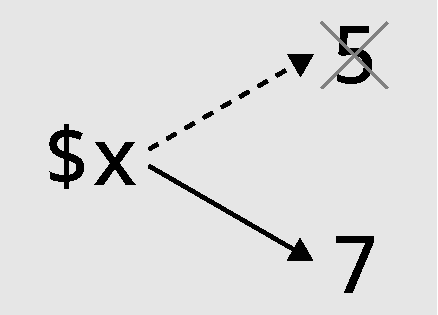
\includegraphics[scale=0.5]{figs/reassignment.pdf}}
\caption{Diagrama de estado.}
\label{fig.assign2}
\end{figure}



\section{Actualización de las Variables}
\label{update}

\index{update}
\index{variable!updating}

Un tipo común de reasignación es una {\bf actualización},
donde el nuevo valor de la variable depende en el viejo:

\begin{verbatim}
> $x = $x + 1;
\end{verbatim}
%
Esto significa ``obtén el valor actual de {\tt \$x}, agrega uno, y después
actualiza {\tt \$x} con el valor nuevo.``

Si intentas actualizar una variable que no se le ha dado un valor,
obtienes una advertencia, porque Perl evalúa el lado derecho de la 
sentencia de asignación antes de que asigne un valor a {\tt \$x}:

\begin{verbatim}
> my $x;
> $x = $x + 1;
Use of uninitialized value of type Any in numeric context 
 in block <unit> at <unknown file> line 1
\end{verbatim}
%
Antes de actualizar una variable, tienes que declararla 
e {\bf inicializarla}, usualmente con una sentencia de asignación:
\index{initialization (before update)}

\begin{verbatim}
> my $x = 0;
> $x = $x + 1;
\end{verbatim}
%
Actualizar una variable al agregar 1 se conoce como un {\bf incremento};
substraer 1 se conoce como un {\bf decremento}.
\index{increment operator}
\index{decrement operator}

Como se mencionó anteriormente en la Sección~\ref{expr_and_statements},
Perl tiene algunos atajos para el incremento y el decremento:

\begin{verbatim}
$x += 1; # equivalente a $x = $x + 1
$x++;    # también equivalente 

$x -= 1; # equivalente a $x = $x - 1
$x--;    # también equivalente 
\end{verbatim}

\section{The {\tt while} Statement}
\index{statement!while}
\index{while loop}
\index{loop!while}
\index{iteration}

Computers are often used to automate repetitive tasks.  Repeating
identical or similar tasks without making errors is something that
computers do well and people do poorly.  In a computer program,
repetition is also called {\bf iteration}.

We have already seen two functions, {\tt countdown} and
\verb"print-n-times", that iterate using recursion 
(see Section~\ref{recursion}).  Because 
iteration is so common, most programming languages including 
Perl provide language features to make it easier.
One is the {\tt for} statement we saw in Section~\ref{for_loops}.
We'll get back to that later.

Another is the {\tt while} statement.  Here is a version of {\tt
countdown} that uses a {\tt while} statement:

\begin{verbatim}
sub countdown(Int $n is copy) {
    while $n > 0 {
        say $n;
        $n--;
    }
    say 'Blastoff!';
}
\end{verbatim}
%
You can almost read the {\tt while} statement as if it were English.
It means, ``While {\tt \$n} is greater than 0,
display the value of {\tt n} and then decrement
{\tt \$n}.  When you get to 0, display the word {\tt Blastoff!}''
\index{flow of execution}

More formally, here is the flow of execution for a {\tt while} statement:

\begin{enumerate}

\item Determine whether the condition is true or false.

\item If false, exit the {\tt while} statement
and continue execution at the next statement.

\item If the condition is true, run the
body and then go back to step 1.

\end{enumerate}

This type of flow is called a loop because the third step
loops back around to the top.  
\index{condition}
\index{loop}
\index{body}

The body of the loop should change the value of one or more variables
so that the condition becomes false eventually and the loop
terminates.  Otherwise, the loop will repeat forever, which is called
an {\bf infinite loop}.  An endless source of amusement for computer
scientists is the observation that the directions on shampoo,
``Lather, rinse, repeat,'' are an infinite loop.
\index{infinite loop}
\index{loop!infinite}

In the case of {\tt countdown}, we can prove that the loop
terminates: if {\tt \$n} is zero or negative, the loop never runs.
Otherwise, {\tt \$n} gets smaller each time through the
loop, so eventually we have to get to 0.

For some other loops, it is not so easy to tell whether the 
loop terminates.  For example:

\begin{verbatim}
sub sequence($n is copy) {
    while $n != 1 {
        say $n;
        if $n %% 2 {        # $n is even
            $n = $n / 2;
        } else {            # $n is odd
            $n = $n*3 + 1
        }
    }
    return $n;
}
\end{verbatim}
%
The condition for this loop is {\tt \$n != 1}, so the loop will continue
until {\tt \$n} is {\tt 1}, which makes the condition false.

Each time through the loop, the program outputs the value of {\tt \$n}
and then checks whether it is even or odd.  If it is even, {\tt \$n} is
divided by 2.  If it is odd, the value of {\tt \$n} is replaced with
{\tt \$n*3 + 1}. For example, if the argument passed to {\tt sequence}
is 42, the resulting values of {\tt n} are 42, 21, 64, 32, 16, 8, 4, 2, 1.

Since {\tt \$n} sometimes increases and sometimes decreases, there is no
obvious proof that {\tt \$n} will ever reach 1, or that the program
terminates.  For some particular values of {\tt n}, we can prove
termination.  For example, if the starting value is a power of two,
{\tt n} will be even every time through the loop
until it reaches 1. The previous example ends with such a sequence
of powers of two, starting with 64.
\index{Collatz conjecture}

The hard question is whether we can prove that this program terminates
for {\em all} positive values of {\tt n}.  So far, no one has
been able to prove it {\em or} disprove it!  (See
\url{http://en.wikipedia.org/wiki/Collatz_conjecture}.)

As an exercise, you might want to rewrite the function 
\verb"print-n-times" from Section~\ref{recursion} using 
iteration instead of recursion.

\index{statement modifier}
\index{postfix!syntax}
The {\tt while} statement can also be used as a statement modifier (or postfix syntax):

\begin{verbatim}
my $val = 5;
print "$val " while $val-- > 0;   # prints 4 3 2 1 0
print "\n";
\end{verbatim}

The {\tt while} loop statement executes the block as long as 
its condition is true. There is also an {\tt until} loop 
statement, which executes the block as long as its condition 
is false:
\index{until loop}

\begin{verbatim}
my $val = 1;
until $val > 5 {
    print $val++;                 # prints 12345
}
print "\n";
\end{verbatim}

\section{Local Variables and Variable Scoping}

We have seen in Section~\ref{localvar} that variables created 
within a subroutine (with the {\tt my} keyword) are \emph{local} 
to that subroutine. The {\tt my} 
keyword is often called a \emph{declarator}, because it 
is used for declaring a new variable (or other identifier). 
It is by far the most common declarator. Other declarators 
include {\tt our} or {\tt state}, briefly described later 
in this chapter. 
\index{lexical scope}
\index{lexical variable}
\index{variable!lexical}
\index{my}
\index{declarator}

Similarly, subroutine 
parameters are also usually \emph{local} to the subroutine 
in the signature of which they are declared.
\index{subroutine parameters}

We briefly mentioned that the term \emph{lexically scoped} 
is probably more accurate than local, but it was 
too early at that point to really explain what this means.

Declaring a variable with {\tt my} gives it \emph{lexical 
scope}. This means it only exists within the current block. 
Loosely speaking, a 
block is a piece of Perl code within curly brackets or 
braces. For example, the body of a subroutine and the code of a 
{\tt while} or {\tt for} loop or of an {\tt if} conditional
statement are code blocks. Any variable created with the 
{\tt my} declarator exists and is available for use only 
between the place where it is declared and the end of the 
enclosing code block.
\index{bracket!curly}
\index{curly bracket}

For example, this code:

\begin{verbatim}
if $condition eq True {
    my $foo = "bar";
    say $foo;  # prints "bar"
}
say $foo;      # ERROR: "Variable '$foo' is not declared ..."
\end{verbatim}
%
will fail on the second print statement, because the \verb'say' 
function call is not in 
the lexical scope of the {\tt \$foo} variable, which ends 
with the closing brace of the condition block. If we want 
this variable to be accessible after the end of the condition, 
then we would need to declare it before the {\tt if} statement. 
For example:

\begin{verbatim}
my $foo;
if $condition eq True {
    $foo = "bar";
    say $foo;  # prints "bar"
} else {
    $foo = "baz";
}
say $foo;      # prints "bar" or "baz" depending on $condition
\end{verbatim}
%
If a lexical variable is not declared within a block, its 
scope will extend until the end of the file (this is sometimes 
called a static or a global variable, although these terms are 
somewhat inaccurate). For example, in the last code snippet 
above, the scope of the {\tt \$foo} variable will extend 
until the end of the file, which may or may not be a good thing, 
depending on how you intend to use it. It 
is often better to reduce the scope of variables as much as 
possible, because this helps reduce dependencies between 
various parts of the code and limits 
the risk of subtle bugs. In the code above, if we want to 
limit the scope of {\tt \$foo}, we could add braces to create 
an enclosing block for the sole purpose of limiting the scope:
\begin{verbatim}
{
    my $foo;
    if $condition eq True {
        $foo = "bar";
        say $foo;  # prints "bar"
    } else {
        $foo = "baz";
    }
    say $foo;      # prints "bar" or "baz" depending on $condition
}
\end{verbatim}
% 
Now, the outer braces create an enclosing block limiting the 
scope of {\tt \$foo} to where we need it. This may seem to be a 
somewhat contrived example, but it is not uncommon to add 
braces only for the purpose of precisely defining the scope 
of something.

Lexical scoping also means that variables with the same names
can be temporarily redefined in a new scope: 

\begin{verbatim}
my $location = "outside";
sub outer {
    say $location;
}
sub inner {
    my $location = "inside";
    say $location;
}
say $location;   # -> outside
outer();         # -> outside
inner();         # -> inside
say $location;   # -> outside
\end{verbatim}
% 
We have in effect two variables with the same name, 
{\tt \$location}, but different scopes. One is valid only 
within the {\tt inner} subroutine where it has been redefined, 
and the other anywhere else.

If we add a new subroutine:
\begin{verbatim}
sub nowhere {
    my $location = "nowhere";
    outer();
}
nowhere();       # -> outside
\end{verbatim}
% 
this will still print ``outside,'' because the {\tt outer} 
subroutine knows about the ``outside'' version of the 
{\tt \$location} variable, which existed when {\tt outer} was defined.
In other word, the {\tt outer} code that referenced to the 
outer variable (``outside'') knows about the variable that existed 
when it was created, but not about the variable existing where 
it was called. This is how \emph{lexical} variables work. 
This behavior is the basis for building \emph{closures}, a  
form of subroutine with some special properties that we 
will study later in this book, but 
is in fact implicitly present everywhere in Perl~6.
\index{closure}
\index{variable!lexical}
\index{lexical variable}

While having different variables with the same name can give 
you a lot of expressive power, we would 
advise you to avoid creating different variables with the 
same name and different scopes, at least until you really understand 
these concepts well enough to know what you are doing, as this 
can be quite tricky.

By far, most variables used in Perl are lexical variables, 
declared with the {\tt my} declarator. Although they are 
not declared with {\tt my}, parameters declared 
in the signature of subroutines and parameters of pointy 
blocks also have a lexical scope limited to the body of the 
subroutine or the code block.
\index{my}
\index{declarator}

There are other declarators, such as {\tt our}, which creates 
a package-scoped variable, and {\tt state}, which creates a 
lexically scoped variable but with a persistent value. They 
are relatively rarely used.
\index{our}
\index{state}

One last point: although they are usually not declared with 
a {\tt my} declarator, subroutines themselves also have by default
a lexical scope. If they are defined within a block, they will 
be seen only within that block. An example of this has been 
given at the end of the solution to the GCD exercise of the 
previous chapter (see Subsection~\ref{sol_gcd}). 
That being said, you \emph{can} declare a subroutine with 
a {\tt my} declarator if you wish:

\begin{verbatim}
my sub frobnicate { 
    # ... 
}
\end{verbatim}

This technique might add some consistency or some form of 
self-documenting feature, but you won't buy very much 
added functionality with that.
 

\section{Control Flow Statements ({\tt last}, {\tt next}, etc.)}
\index{control flow}
\index{flow!control}
\index{last statement}
\index{statement!last}
\index{next statement}
\index{statement!next}

Sometimes you don't know it's time to end a loop until you get half
way through the body.  In that case, you can use a control flow 
statement such as {\tt last} to jump out of the loop.

For example, suppose you want to take input from the user until they
type {\tt done}.  You could write:

\begin{verbatim}
while True {
    my $line = prompt "Enter something ('done' for exiting)\n";
    last if $line eq "done";
    say $line;
}
say 'Done!';
\end{verbatim}
%
The loop condition is {\tt True}, which is always true, so the
loop runs until it hits the {\tt last} statement.

Each time through, it prompts the user to type something.
If the user types {\tt done}, the {\tt last} statement exits
the loop.  Otherwise, the program echoes whatever the user types
and goes back to the top of the loop.  Here's a sample run:

\begin{verbatim}
$ perl6 while_done.pl6
Enter something ('done' for exiting)
Not done
Not done
Enter something ('done' for exiting)
done
Done!
\end{verbatim}
%
This way of writing {\tt while} loops is common because you
can check the condition anywhere in the loop (not just at the
top) and you can express the stop condition affirmatively
(``stop when this happens'') rather than negatively (``keep 
going until that happens'').

Using a {\tt while} loop with a condition that is always true 
is a quite natural way of writing an infinite loop, i.e., a 
loop that will run forever until something else in the code 
(such as the {\tt last} statement used above) forces the 
program to break out of the loop. This is commonly used in 
many programming languages, and this works well in Perl. There 
is, however, another common and more idiomatic way of constructing 
infinite loops in Perl~6: using the {\tt loop} statement, 
which we will study in Section~\ref{C-style loop} 
(p.~\pageref{C-style loop}). For now, we'll use the {\tt while True} 
statement, which is fairly legitimate.
\index{idiomatic}
\index{loop!infinite}
\index{infinite loop}

Sometimes, rather than simply breaking out of the {\tt while}  loop 
as with the {\tt last} control statement, you need to start the 
body of the loop at the beginning. For example, you may want 
to check whether the user input is correct with some 
(unspecified) {\tt is-valid} subroutine before processing 
the data, and ask the user to try again if the input was not 
correct. In this case, the {\tt next} control statement lets 
you start at the top the loop body again:
\index{next statement}
\index{statement!next}

\begin{verbatim}
while True {
    my $line = prompt "Enter something ('done' for exiting)\n";
    last if $line eq "done";
    next unless is-valid($line);
    # further processing of $line;
}
print('Done!')
\end{verbatim}
%
Here, the loop terminates if the user types ``done.'' If not, the user input is checked by the {\tt is-valid} subroutine; if the subroutine returns a true value, the processing continues forward; if it returns a false value, then the control flow starts again at the beginning of the body of the loop, so the user is prompted again to submit a valid input.

The {\tt last} and {\tt next} control statements also work in 
{\tt for} loops. For example, the following {\tt for} loop 
iterates in theory on a range of integer numbers between 1 and 20, 
but discards odd numbers by virtue of a {\tt next} statement 
and breaks out of the loop with a {\tt last} statement as 
soon as the loop variable is greater than {\tt \$max} (i.e., 10 in this  example):
\index{for loop}
\index{loop!for}
\index{statement!for}

\begin{verbatim}
my $max = 10;
for 1..20 -> $i {
    next unless $i %% 2; # keeps only even values
    last if $i > $max;   # stops loop if $i is greater than $max
    say $i;              # prints 2 4 6 8 10
}
\end{verbatim}

You may have as many {\tt last} and {\tt next} statements as you 
like, just as you may have as many {\tt return} statements as 
you like in a subroutine. Using such control flow statements 
is not considered poor 
practice. During the early days of structured programming, 
some people insisted that loops and subroutines have only one 
entry and one exit. The one-entry notion is still a good idea, 
but the one-exit notion has led people to bend over backwards 
and write a lot of unnatural code. Much of programming consists of traversing 
decision trees. A decision tree naturally starts with a single 
trunk but ends with many leaves. Write your code with the number 
of loop controls (and subroutine exits) that is natural to the 
problem you're trying to solve. If you've declared your variables 
with reasonable scopes, everything gets automatically cleaned up 
at the appropriate moment, no matter how you leave the block.


\section{Square Roots}
\label{squareroot}
\index{square root}

Loops are often used in programs that compute
numerical results by starting with an approximate answer and
iteratively improving it.
\index{Newton's method}

For example, one way of computing square roots is Newton's 
method (also known as the Newton-Raphson's method).
Suppose that you want to know the square root of $a$.  If you start
with almost any estimate, $x$, you can compute a better
estimate $y$ with the following formula:

\[ y = \frac{x + a/x}{2} \]
%
For example, if $a$ is 4 and $x$ is 3:

\begin{verbatim}
> my $a = 4;
4
> my $x = 3;
3
> my $y = ($x + $a/$x)/2;
2.166667
\end{verbatim}
%
The result is closer than 3 to the correct answer 
($\sqrt{4} = 2$) .  If we repeat the process with the new estimate, it gets even closer:

\begin{verbatim}
> $x = $y;
2.166667
> $y = ($x + $a/$x)/2;
2.006410
\end{verbatim}
%
After a few more updates, the estimate is almost exact:
\index{update}

\begin{verbatim}
> $x = $y;
2.006410
> $y = ($x + $a/$x)/2;
2.000010
> $x = $y;
2.000010
> $y = ($x + $a/$x)/2;
2.000000000026
\end{verbatim}
%
In general we don't know ahead of time how many steps it takes
to get to the right answer, but we know when we get there
because the estimate stops changing:

\begin{verbatim}
> $x = $y;
2.000000000026
> $y = ($x + $a/$x)/2;
2
> $x = $y;
2
> $y = ($x + $a/$x)/2;
2
\end{verbatim}
%
When {\tt \$y == \$x}, we can stop.  Here is a loop that starts
with an initial estimate, {\tt x}, and improves it until it
stops changing:

\begin{verbatim}
my ($a, $x) = (4, 3);
while True {
    say "-- Intermediate value: $x";
    my $y = ($x + $a/$x) / 2;
    last if $y == $x;
    $x = $y;
}
say "Final result is $x";
\end{verbatim}
%
This will print:
\begin{verbatim}
-- Intermediate value: 3
-- Intermediate value: 2.166667
-- Intermediate value: 2.006410
-- Intermediate value: 2.000010
-- Intermediate value: 2.000000000026
-- Intermediate value: 2
Final result is 2
\end{verbatim}
%

For most values of {\tt \$a} this works fine, but there are a 
couple of caveats with this approach. First, in most programming 
languages, it is dangerous to test {\tt float} equality, because 
floating-point values are only approximately right. We do not 
have this problem with Perl~6, because, as we have already 
mentioned, it is using a better representation of rational 
numbers than most generalist programming languages. (You 
may want to keep this in mind if you are using some other
languages.) Even if we don't have this problem with Perl, there 
may also be some problems with algorithms that do not behave 
as well as Newton's algorithm. For example, some algorithms 
might not converge as fast and as neatly as Newton's algorithm but might instead produce alternate values above and below the accurate result.
\index{floating-point}
\index{epsilon}

Rather than checking whether {\tt \$x} and {\tt \$y} are exactly equal, it
is safer to use the built-in function {\tt abs} to compute the
absolute value, or magnitude, of the difference between them:

\begin{verbatim}
    last if abs($y - $x) < $epsilon:
\end{verbatim}
%
where \verb"epsilon" has a very small value like {\tt 0.0000001} 
that determines how close is close enough.



\section{Algorithms}
\index{algorithm}

Newton's method is an example of an {\bf algorithm}: it is a
mechanical process for solving a category of problems (in this
case, computing square roots).

To understand what an algorithm is, it might help to start with
something that is not an algorithm.  When you learned to multiply
single-digit numbers, you probably memorized the multiplication table.
In effect, you memorized 100 specific solutions.  That kind of
knowledge is not algorithmic.

But if you were ``lazy,'' you might have learned a few
tricks.  For example, to find the product of $n$ and 9, you can
write $n-1$ as the first digit and $10-n$ as the second
digit.  (For example, to figure out $9*7$, $n-1$ is 6 and 
$10-n$ is 3, so that the product $9*7$ is 63.) This trick 
is a general solution for multiplying any single-digit 
number by 9.  That's an algorithm!
\index{addition with carrying}
\index{carrying, addition with}
\index{subtraction!with borrowing}
\index{borrowing, subtraction with}

Similarly, the techniques you learned in school for addition 
(with carrying), subtraction (with borrowing), and long 
division are all algorithms.  One
of the characteristics of algorithms is that they do not require any
intelligence to carry out.  They are mechanical processes where
each step follows from the last according to a simple set of rules.

Executing algorithms is boring, but designing them is interesting,
intellectually challenging, and a central part of computer science.

Some of the things that people do naturally, without difficulty or
conscious thought, are the hardest to express algorithmically.
Understanding natural language is a good example.  We all do it, but
so far no one has been able to explain {\em how} we do it, at least
not in the form of an algorithm.


\section{Debugging}
\label{bisectbug}

As you start writing bigger programs, you might find yourself
spending more time debugging.  More code means more chances to
make an error and more places for bugs to hide.
\index{debugging!by bisection}
\index{bisection, debugging by}

One way to cut your debugging time is ``debugging by bisection.''
For example, if there are 100 lines in your program and you
check them one at a time, it would take 100 steps.

Instead, try to break the problem in half.  Look at the middle
of the program, or near it, for an intermediate value you
can check.  Add a {\tt say} statement (or something else
that has a verifiable effect) and run the program.

If the midpoint check is incorrect, there must be a problem in the
first half of the program.  If it is correct, the problem is
in the second half.

Every time you perform a check like this, you halve the number of
lines you have to search.  After six steps (which is fewer than 100),
you would be down to one or two lines of code, at least in theory.

In practice it is not always clear what
the ``middle of the program'' is and not always possible to
check it.  It doesn't make sense to count lines and find the
exact midpoint.  Instead, think about places
in the program where there might be errors and places where it
is easy to put a check.  Then choose a spot where you
think the chances are about the same that the bug is before
or after the check.


\section{Glossary}

\begin{description}

\item[Reassignment] Assigning a new value to a variable that
already exists.
\index{reassignment}

\item[Update] An assignment where the new value of the variable
depends on the old.
\index{update}

\item[Initialization] An assignment that gives an initial value to
a variable that may later be updated.
\index{initialization!variable}

\item[Increment] An update that increases the value of a variable
(often by one).
\index{increment operator}

\item[Decrement] An update that decreases the value of a variable.
\index{decrement operator}

\item[Iteration] Repeated execution of a set of statements using
either a recursive function call or a loop.
\index{iteration}

\item[Infinite loop] A loop in which the terminating condition is
never satisfied.
\index{infinite loop}
\index{loop!infinite}

\item[Algorithm]  A general process for solving a category of
problems.
\index{algorithm}

\end{description}


\section{Exercises}

\begin{exercise}
\label{test_sqrt}
\index{square root}
\index{algorithm!square root}

Copy the loop from Section~\ref{squareroot}
and encapsulate it in a subroutine called
\verb"my-sqrt" that takes {\tt \$a} as a parameter, chooses a
reasonable value of {\tt \$x}, and returns an estimate of 
the square root of {\tt \$a}.

To test it, write a function named \verb"test-square-root"
that prints a table like this:

\begin{verbatim}[fontshape=up]
a  mysqrt(a)        sqrt(a)          diff
1  1.0000000000000  1.0000000000000  1.110223e-15
2  1.4142135623747  1.4142135623731  1.594724e-12
3  1.7320508075689  1.7320508075689  0.000000e+00
4  2.0000000000000  2.0000000000000  0.000000e+00
5  2.2360679774998  2.2360679774998  0.000000e+00
6  2.4494897427832  2.4494897427832  8.881784e-16
7  2.6457513110647  2.6457513110646  1.025846e-13
8  2.8284271247494  2.8284271247462  3.189449e-12
9  3.0000000000000  3.0000000000000  0.000000e+00

\end{verbatim}
%
The first column is a number, $a$, the second column is the 
square root of $a$ computed with \verb"my-sqrt", the third 
column is the square root computed by the {\tt sqrt} built-in 
function of Perl, and the fourth column is the absolute value of 
the difference between the two estimates. Don't worry too much about 
obtaining a clean tabular formatting, we haven't 
seen the built-in functions to do that. 

Solution: \ref{sol_test_sqrt}
%

\end{exercise}



\begin{exercise}
\index{Ramanujan, Srinivasa}
\index{Ramanujan, Srinivasa!pi estimate}
\index{pi!estimate}
\label{pi_estimate}

The mathematician Srinivasa Ramanujan found an infinite 
series that can be used to generate a numerical
approximation of $1 / \pi$:
\index{pi}

\[ \frac{1}{\pi} = \frac{2\sqrt{2}}{9801} 
\sum^\infty_{k=0} \frac{(4k)!(1103+26390k)}{(k!)^4 396^{4k}} \]

Write a function called \verb"estimate-pi" that uses this 
formula to compute and return an estimate of $\pi$.  It 
should use a {\tt while} loop to compute terms of the 
summation until the last term is smaller than {\tt 1e-15} 
(which is Perl notation for $10^{-15}$). You can check
the result by comparing it to the built-in constant {\tt pi}.
Solution: \ref{sol_pi_estimate}.

\end{exercise}




\chapter{Cadenas de texto}
\label{strings}
\index{string}

Las cadenas de texto no son como los enteros, los racionales,
y los Booleanos. Una cadena de texto es una {\bf secuencia} de caracteres,
lo cual significa que es una colección ordenada de otros valores,
y algunas veces necesitas acceder algunos de estos valores individuales.
En este capítulo verás cómo analizar, manejar, y modificar cadenas
de texto, y aprenderás sobre algunos de los métodos que las
cadenas de texto proveen. También aprenderás sobre una
herramienta muy poderosa para la manipulación de texto, 
expresiones regulares (también conocidas como ``regexes``).
\index{sequence}
\index{regex}


\section{Una Cadena de Texto es una Secuencia}

\index{sequence}
\index{character}
\index{bracket operator}
\index{operator!bracket}
Una cadena de texto es primariamente una pieza de datos textuales,
pero es técnicamente una secuencia ordenada de caracteres.

Muchos lenguajes de programación te permiten acceder caracteres
individuales de una cadena de texto con índice entre corchetes. 
Esto no es directamente posible en Perl, pero todavía puedes
los caracteres uno a la vez usando el método integrado {\tt comb} 
y el operador corchete:

\begin{lstlisting}
> my $cadena = "banana";
banana
> my $cad = $cadena.comb;
(b a n a n a)
> say $cad[1];
a
> say $cad[2];
n
\end{lstlisting}
%
El método {\tt comb} en la segunda sentencia divide la cadena de texto
en una lista de caracteres que puedes acceder individualmente con
los corchetes.
\index{comb function and method}
\index{method!comb}
\index{function!comb}
\index{bracket!square}
\index{square bracket operator}
\index{index}
\index{subscript}

La expresión dentro de los corchetes se llama un {\bf índice}
(también llamado subíndice). El índice indica cuales 
caracteres en la secuencia quieres (de ahí el nombre). Pero
puede ser que esto no es lo que esperabas: el artículo con
índice 1 es la segunda letra de la palabra. Para los
científicos de la computación, el índice es usualmente
un desplazo del inicio. Por ejemplo, el índice de la primera 
letra (``b``) es 0, y el índice de la primera ``a`` es 1,
no 2, etcétera.
\index{index!starting at zero}
\index{zero, index starting at}

También podrías extraer una ``rebanada`` de varios caracteres
de una sola vez al usar el operador de rango dentro de los 
corchetes:
\index{slice}

\begin{lstlisting}
> say $cad[2..5]
(n a n a)
\end{lstlisting}
%
\index{substring}
De nuevo, la subcadena ``nana`` comienza en la tercera letra
de \verb|'banana'|, pero esta letra está indexada 2, y la
sexta letra tiene índice 5.

Aunque esto puede ser útil en ocasiones, esta no es la manera
en la que manejarías cadenas de texto en Perl, el cual tiene
herramientas superiores que son más poderosas y más 
expresivas, así que raramente necesitas usar índices o 
subíndices para acceder caracteres individuales.

También, si existe una necesidad real de acceder y manipular
las letras individuales, haría más sentido almacenarlas en un 
array, pero no hemos hablado sobre arrays todavía, así que
regresaremos a esto más tarde.

\section{Operadores Comunes de Cadenas de Texto}
\index{string!operators}

Perl provee un número de operadores y funciones para el 
manejo de cadenas de texto. Revisemos algunos de los más 
populares.

\subsection{Longitud de una Cadena de Texto}
\index{chars function}
\index{function!chars}
\index{string!length}

La primera cosa que desearíamos saber sobre una cadena de texto 
es su longitud. El método (o función) {\tt chars} devuelve el número de
caracteres de una cadena de texto. Como podemos ver, {\tt chars} puede
usarse con una sintaxis de método o función:
\index{invocation!method}
\index{method invocation}

\begin{lstlisting}
> say "banana".chars;   # sintaxis de invocación de método
6
> say chars "banana";   # sintaxis de llamada de función
6
\end{lstlisting}
%

\index{Unicode}
\index{grapheme}
Nota que, con el advenimiento de Unicode, la noción 
sobre la longitud de una cadena de texto se ha vuelto 
más complicada que lo era con cadenas de texto ASCII.
Hoy en día, un carácter puede estar compuesto de uno, dos, o 
más bytes. La rutina {\tt chars} devuelve el número de 
caracteres (en el sentido de los grafemas de Unicode, los cuales
son más o menos lo que los humanos perciben como caracteres) dentro
de la cadena, aún cuando algunos caracteres requieren una
codificación de más de 2, 3, o 4 bytes.

Una cadena de texto con una longitud cero (i.e., sin caracteres) se
conoce como una \emph{cadena de texto vacía}.

\subsection{Búsqueda de una Subcadena Dentro de una Cadena de Texto}
\label{find}
\index{index function}
\index{function!index}
\index{substring}

La función integrada {\tt index} usualmente toma dos argumentos,
una cadena de texto y una subcadena (algunas veces conocidas como
la ``paja`` y la ``aguja``), busca la subcadena en la cadena de texto,
y devuelve la posición donde se encuentra la subcadena. Si la subcadena
no se encuentra en la cadena, la función devuelve un valor indefinido:

\begin{lstlisting}
> say index "naranja", "ra";
2
> say index "naranja", "je";
Nil
\end{lstlisting}
%

\index{offset}
Nuevamente, el índice es un desplazo del inicio de la cadena 
de texto, así que el índice de la primera letra (``n``) es cero,
y el índice de la segunda ``a`` es 3, no 4.
\index{index!starting at zero}

También puedes invocar a {\tt index} con una sintaxis de método:
\begin{lstlisting}
> say "naranja".index("ra");
2
\end{lstlisting}
%

La función {\tt index} puede tomar un tercer argumento opcional,
un entero que indica donde comenzar la \emph{búsqueda} (y por lo
tanto ignorando en la búsqueda cualquier carácter posterior a
la posición de inicio):

\begin{lstlisting}
> say index "naranja", "a", 2;
3
\end{lstlisting}
%
Aquí la función {\tt index} comenzó la búsqueda en la ``r`` y encontró 
la posición de la segunda ocurrencia de la subcadena ``a``.
 

\index{function!rindex}
\index{rindex function}
También existe una función {\tt rindex}, la cual realiza la búsqueda
de la subcadena de atrás hacia adelante y devuelve la última posición de 
la subcadena dentro de la cadena de texto:

\begin{lstlisting}
> say rindex "naranja", "a";
6
\end{lstlisting}
%

Nota que aunque {\tt rindex} inspecciona la cadena de texto
de atrás hacia adelante, la función devuelve una posición
computada desde el inicio de la cadena de texto.

\subsection{Extrayendo una Subcadena de una Cadena de Texto}
\index{substr function or method}
\index{function!substr}
\index{substring}

La función opuesta a {\tt index} es la función (o método) {\tt substr},
la cual, dada una posición inicial y una longitud, extrae una subcadena
de una cadena de texto:

\begin{lstlisting}
> say substr "Hacer es la mejor manera de decir.", 0, 5;
Hacer
> say "Hacer es la mejor manera de decir.".substr(12, 5)
mejor
\end{lstlisting}
%

\index{chars function}
\index{Unicode}
\index{grapheme}
Nota que, al igual que la función {\tt chars}, la longitud es
expresada en caracteres (o grafemas Unicode), no en bytes.
De igual modo, como puedes observar, los espacios que separan
las palabras dentro de la cadena de texto obviamente cuentan 
como caracteres. El argumento de la longitud es opcional; 
si no se provee, la función {\tt substr} devuelve la subcadena
comenzando en la posición de inicio al final de la cadena de texto:

\begin{lstlisting}
> say "Hacer es la mejor manera de decir.".substr(9)
la mejor manera de decir.
\end{lstlisting}

Similamente, si el valor de la longitud es muy largo para que 
la subcadena comience en la posición inicial, la función
{\tt substr} devolverá la subcadena comenzando en la posición
inicial hasta el final de la cadena:

\begin{lstlisting}
> say substr "banana", 2, 10;
nana
\end{lstlisting}

Por supuesto, los parámetros de la posición inicial y la longitud 
no necesitan números literales como en los ejemplos anteriores; puedes
también usar variables (o hasta una expresión o una función que devuelve 
un valor numérico), provisto que la variable o la función pueda ser 
coaccionada en un entero. Pero la posición de inicio debe estar dentro 
del rango de la cadena de texto, y si falla obtienes un error 
{\tt Start argument to substr out of range ...}; por lo tanto
podrías tener que verificarlo en contra de la longitud de la 
cadena de texto con antelación.

También puedes comenzar a contar de atrás hacia adelante con la
siguiente sintaxis:

\begin{lstlisting}
> say "I have a dream".substr(*-5)
dream
> say substr "I have a dream", *-5;
dream
\end{lstlisting}
%
Aquí, el asterisco * puede considerarse como una representación de la
longitud total de la cadena de texto; \verb|*-5| es por lo tanto la posición
en la cadena de texto cinco caracteres antes del final de la cadena. Así que
\verb|substr(*-5)| devuelve los caracteres desde esa posición hasta el final
de la cadena de texto, i.e., los últimos cinco caracteres de la cadena de
texto.
\index{substr function}
\index{substring}

\subsection{Otras Funciones o Métodos Útiles de Cadenas de Texto}
\index{string!operators}

Esto puede no ser obvio todavía, pero prontamente veremos
que la combinación de las funciones de cadenas de texto que discutimos
más arriab nos dan ya mucho poder para manipular cadenas de texto
más allá de lo que piensas posible en este punto.

Déjanos mencionar brevemente varias funciones adicionales
que pueden ser útiles de vez en cuando.

\subsubsection{flip}

\index{flip function}
\index{function!flip}
La función (o método) {\tt flip} invierte una cadena de texto:

\begin{lstlisting}
> say flip "mango";
ognam
\end{lstlisting}
%

\subsubsection{split}
\index{split function or method}
\index{function!split}
\index{delimiter}
La función (o método) {\tt split} divide una cadena de texto 
en subcadenas de texto, basado en los delimitadores en l
cadena de texto:

\begin{lstlisting}
> say $_ for split "-", "25-12-2016";
> #                 ^ delimitador
25
12
2016
> for "25-12-2016".split("-") -> $val {say $val};
25
12
2016
\end{lstlisting}

El delimitador puede ser un solo carácter con comillas como
en el ejemplo más arriba o una cadena de varios caracteres, 
tales como una coma y un espacio en el ejemplo más abajo:

\begin{lstlisting}
> .say for split  ", ", "Jan, Feb, Mar";
> #                ^^ delimitador
Jan
Feb
Mar
\end{lstlisting}

Recuerda que \verb|.say| es un atajo para \verb|$_.say|.

Por defecto, los delimitadores no aparecen en la salida producida por 
la función (o método) {\tt split}, pero este comportamiento puede 
cambiarse con el uso de {\tt adverbio} apropiado. Un adverbio es básicamente
un argumento nombrado de una función que modifica la manera en la 
función se comporta. Por ejemplo, el adverbio {\tt :v} (valores)
le dice a {\tt split} que también devuelva el valor del delimitador:
\index{adverb}
\index{:v adverb}

\begin{lstlisting}
> .perl.say for split  ', ', "Jan, Feb, Mar", :v;
"Jan"
", "
"Feb"
", "
"Mar"
\end{lstlisting}

Los otros adverbios que pueden usarse en este contexto son {\tt :k} (claves), 
{\tt :kv} (claves y valores), y {\tt :p} (pares). Su significados detallados pueden
encontrarse en la documentación para {\tt split}
(\url{https://docs.perl6.org/routine/split}). El adverbio {\tt skip-empty}
remueve las partes vacías de la lista de resultados.

La función {\tt split} pueden también usarse un \emph{patrón} 
de expresión regular como un delimitador, y esto puede hacerla
mucho más poderosa. Estudiaremos expresiones regulares más adelante
en este capítulo.
\index{regular expression}
\index{regex}

\subsubsection{Concatenación de Cadenas de Texto}

\index{concatenate operator}
\index{string!concatenation}
\index{string concatenation}

El operador \verb|~| concatena dos cadenas de texto y forma una:

\begin{lstlisting}
> say "ban" ~ "ana";
banana
\end{lstlisting}
%

Puedes tener cadenas de varias ocurrencias de este operador
para concatenar más de dos cadenas:

\begin{lstlisting}
> say "ba" ~ "na" ~ "na";
banana
\end{lstlisting}
%

Si se usa como un operador prefijo unario,
\verb|~| transforma su argumento en una cadena de texto:
\index{stringify operator}
\index{stringification}

\begin{lstlisting}
> say (~42).WHAT;
(Str)
\end{lstlisting}
%

\subsubsection{Separando en Palabras}

\index{words function or method}
La función {\tt words} devuelve una lista de palabras
que componen la cadena de texto:

\begin{lstlisting}
> say "I have a dream".words.perl;
("I", "have", "a", "dream").Seq
> .say for "I have a dream".words;
I
have
a
dream
\end{lstlisting}
%

\subsubsection{join}

\index{join function or method}
\index{function!join}
La función {\tt join} toma un argumento separador y una lista
de cadenas de texto como argumentos; la función las intercala
con el separador, concatena todo en una sola cadena de texto, y 
devuelve la cadena de texto resultante.

Este ejemplo ilustra el uso de las funciones (o métodos) 
{\tt words} y {\tt join}:

\begin{lstlisting}
say 'I have a dream'.words.join('|');    # -> I|have|a|dream
say join ";", words "I have a dream";    # -> I;have;a;dream
\end{lstlisting}
%

\index{words function or method}
En ambos casos, {\tt words} primero divide la cadena original
en una lista de palabras,  {\tt splits} sutura los artículos
de esta lista y los devuelve en una nueva cadena de texto 
intercalados con el separador.

\subsubsection{Conversión a Minúscula y a Mayúscula}
\index{lc function or method} 
\index{lower case!lc function}
\index{uc function or method}
\index{tc function or method}
\index{upper case}
\index{lower case}
\index{title case}
\index{case!upper}
\index{case!lower}
\index{case!title}

Las rutinas {\tt lc} y {\tt uc} devuelven respectivamente
una versión en minúscula y una versión mayúscula de sus 
argumentos. También está la función {\tt tc} la cual devuelve
su argumento con la primera letra en mayúscula:

\begin{lstlisting}
say lc "Abril";    # -> april
say "Abril".lc;    # -> april
say uc "abril";    # -> APRIL
say tc "abril";    # -> April
\end{lstlisting}

\index{eq, string equality operator}
Recuerda que el operador {\tt eq} chequea la igualdad de dos 
cadenas de texto.

\section{Recorrido de una Cadena con un bucle {\tt while} o {\tt for}}
\label{stringtraversal}
\index{traversal}
\index{loop!traversal}
\index{for loop}
\index{loop!for}
\index{statement!for}
\index{index function}
\index{while loop}

Muchas computaciones involucran el procesamiento de una
cadena de texto una carácter a la vez. Usualmente ellas
comienzan al principio, seleccionan cada carácter en turno,
hacen algo con dicho carácter, y continúan hasta el final.
Este patrón de procesamiento se conoce como {\bf recorrido}. 
Una manera de escribir un recorrido es con un bucle {\tt while}
y la función {\tt index}:
\index{while loop}
\index{index}

\begin{lstlisting}
my $indice = 0;
my $fruta = "banana";
while $indice < $fruta.chars { 
    my $letra = substr $fruta, $indice, 1; 
    say $letra; 
    $indice++;
}
\end{lstlisting}
%

Esto imprimirá cada letra, una a la vez:
\begin{lstlisting}
b
a
n
a
n
a
\end{lstlisting}
%
Este bucle recorre la cadena de texto y muestra cada letra
en un línea por si misma. La condición del bucle es 
{\tt \$indice < \$fruta.chars},
así que cuando {\tt \$indice} es igual a la longitud de
la cadena de texto, la condición es falsa, y el cuerpo del
bucle no se ejecuta. En otras palabras, el bucle para cuando
{\tt \$indice} es la longitud de la cadena de texto menos 
uno, lo cual corresponde al último carácter de la cadena 
de texto.

Como ejercicio, escribe una función que toma una cadena de 
texto como un argumento y muestra las letras de atrás hacia
adelante, una por línea. Hazlo por lo menos una vez sin utilizar
la función {\tt flip}. Solución: \ref{sol_stringtraversal}

Otra forma de escribir un recorrido es con un bucle {\tt for}:
\index{for loop}
\index{comb function and method}

\begin{lstlisting}
my $fruta = "banana";
for $fruta.comb -> $letra {
    say $letra
}
\end{lstlisting}
%

Cada vez a través del bucle, el siguiente carácter en la
cadena de texto es asignado a la variable {\tt \$letra}.
El bucle continúa hasta que no hayan más caracteres.

El bucle podría también usar la función {\tt substr}:
\index{index function}

\begin{lstlisting}
for 0..$fruta.chars - 1 -> $indice {
    say substr $fruta, $indice, 1;
}
\end{lstlisting}
%

\index{concatenation}
\index{abecedarian}
\index{aphabetic order}
\index{McCloskey, Robert}

El siguiente ejemplo muestra cómo usar concatenación y
un bucle {\tt for} para genera una serie de abecedario (
es decir, en orden alfabético). En el libro 
{\em Make Way for Ducklings} de McCloskey, los nombres de los
patitos son Jack, Kack, Lack, Mack, Nack, Ouack, Pack, y Quack. 
Este bucle podría muestra estos nombres en orden:

\begin{lstlisting}
my $sufijo = 'ack';
for 'J'..'Q' -> $letra {
    say $letra ~ $sufijo;
}
\end{lstlisting}
%
La salida es:

\begin{lstlisting}
Jack
Kack
Lack
Mack
Nack
Oack
Pack
Qack
\end{lstlisting}
%
Por supuesto, esto no es del todo correcto dado que ``Ouack'' y 
``Quack'' están mal escritos. Como ejercicio, modifica el programa
para arreglar este error. Solución: \ref{sol_ducklings}.


\section{Bucles y Conteo}
\label{counter}
\index{counter}
\index{counting and looping}
\index{looping and counting}
\index{looping!with strings}

El siguiente programa cuenta el número de veces que 
la letra ``a`` aparece en una cadena de texto:
\index{comb function and method}

\begin{lstlisting}
my $palabra = 'banana';
my $conteo = 0;
for $palabra.comb -> $letra {
    $conteo++ if $letra eq 'a';
}
say $conteo;              # -> 3
\end{lstlisting}
%

\index{counter}
Este programa demuestra otro patrón de la computación 
llamado {\bf contador}. La variable \verb|$conteo| se inicializa
a 0 y después se incrementa por uno cada vez que se encuentra
una ``a``. Cuando el bucle termina, \verb|$conteo| contiene
el resultado---el número total de ocurrencias de la letra ``a``.
\index{incrementation}

\index{encapsulation}
Como ejercicio, encapsula este código en una subrutina llamada
{\tt contar}, y generalízala para que acepte una cadena de texto 
y la letra a contar como argumentos. Solución: \ref{sol_count_letters}.
\label{count_letters}

\section{Expresiones Regulares (Regexes)}
\label{regex}
\index{regex}
\index{regular expression}

Las funciones y los métodos de cadenas de texto que hemos visto
hasta ahora son realmente poderosos, y pueden usarse para un 
sin número de operaciones relacionadas con la 
manipulación de cadenas de texto. Pero supón que quieres extraer
de la cadena ``yellow submarine`` cualquier letra después
de la letra ``l`` y antes de la letra ``w``. Este tipo de 
``búsqueda difusa`` puede hacerse con un bucle, pero no 
es práctico. Puedes hacerlo como un ejercicio si deseas,
pero debo advertirte: es algo delicado y difícil. Aún si 
no lo haces, la solución puede interesarte: 
ver Subsección\ref{sol_regex_loop}. 
\label{regex_loop}

Si agregas otra condición, por ejemplo que esta letra 
debería extraerse o \emph{capturarse} (i.e. almacenada para 
uso futuro) solo si el resto de la cadena de texto contiene
la subcadena ``rin``, esto comienza a ser algo tedioso. También,
cualquier cambio a los requerimientos conduce a que tengamos
que hacer una reescritura substancial o hasta refactorizar
el código completamente.

Para este tipo de trabajo, una {\bf expresión regular} 
o un {\bf regex} es una herramienta mucha más poderosa
y expresiva. La siguiente es una manera de extraer letras usando
el criterio descrito anteriormente: 


\begin{lstlisting}
> my $cadena = "yellow submarine";
yellow submarine
> say ~$0 if $cadena ~~ / l (.) w .*? rin /;
o
\end{lstlisting}

No te preocupes si no entiendes este ejemplo;
afortunadamente todo se aclarará muy pronto.

\index{operator!smart match}
\index{smart match operator}
El operador \verb|~~| se conoce como el operador de coincidencia
inteligente. Es un operador de relación muy poderoso que puede
usarse para tareas de comparación más avanzadas. En este caso, 
el operador chequea si la variable {\tt \$cadena} a su izquierda
``coincide`` con la expresión a su derecha, i.e., como una 
primera aproximación, si la expresión a su derecha describe la 
cadena de texto (o parte de la misma).

\index{pattern}
La parte \verb|/ l (.) w .*? rin /| se llama un patrón de regex y puede
describirse así: la letra ``l``, seguida por cualquier otro carácter (el
punto) para ser capturado (gracias a los paréntesis), seguida por la
letra ``w``, seguida por un número no específico de caracteres,
seguida por la subcadena ``rin``. !`Uff! !`Todo esto en una sola línea
de código! Bien poderoso, no lo crees? Si la cadena de texto coincide 
con el patrón, entonces la coincidencia devolverá un valor verdadero y 
la variable \verb|$0| será poblada con el carácter a ser capturado---
la letra ``o`` en este caso.
\index{capture}

A menos que sea especificado (veremos cómo hacerlo luego),
los espacios en blanco no son significativos dentro de un 
patrón de regex. Así que puedes agregar espacios dentro de una patrón
para separar sus piezas y hacer tus intenciones más claras.

La mayor parte de este capítulo discutirá los fundamentos de 
la construcción de tales patrones de regex y cómo usarlos. 
Pero el concepto de los regexes es tan crucial en Perl que 
dedicaremos un capítulo completo a este tema y otros asuntos
relacionados (Capítulo~\ref{regex_grammars}).

La noción de la expresiones regulares es originalmente un 
concepto procedente de las teoría de lenguajes formales. 
El primer uso de expresiones regulares en la computación fue 
en las utilidades Unix, algunas de las cuales permanecen en 
extenso uso hoy en día, tales como {\tt grep}, creada por Ken Thomson en 1973,
{\tt sed} (ca. 1974), y {\tt awk}, desarrollada años más tarde (en 1977)
por  Aho, Weinberger, and Kernighan. 
Las versiones anteriores del lenguaje Perl en el decenio del 1980
incluían una versión extendida de las expresiones regulares, que 
ha sido desde tal entonces imitada por muchos otros lenguajes de
programación. La diferencia, no obstante, es que las expresiones
regulares están profundamente arraigadas en el núcleo del lenguaje
Perl, mientras que los otros lenguajes las han adoptado como un
add-on o plug-in, usualmente basado o derivado de una librería 
conocida como Expresiones Regulares Compatible con Perl (PCRE 
por sus siglas en inglés).
\index{awk}
\index{grep}
\index{Thomson, Ken}
\index{sed}
\index{Aho, Alfred}
\index{Weinberger, Peter}
\index{Kernighan, Brian}
\index{PCRE (Perl Compatible Regular Expressions)}
\index{Perl Compatible Regular Expressions (PCRE)}

Las expresiones regulares de Perl han extendido estas nociones
tanto que tienen muy poco que ver con el concepto original de 
teoría de lenguaje , y por lo tanto se ha considerado 
apropiado parar de llamarlas \emph{expresiones regulares}
y hablar de \emph{regexes}, i.e., un tipo de sub-lenguaje
de coincidencia de patrón que funciona de manera similar
a las expresiones regulares.

\section{Uso de los Regexes}
\label{using_regexes}
\index{smart match operator}

Una manera simple de usar un regex es utilizar el operador
de coincidencia inteligente \verb|~~|:
\index{smart match operator}
\index{operator!smart match}

\begin{lstlisting}
say "Coincidió" if "abcdef" ~~ / bc.e /;     # -> Coincidió
\end{lstlisting}
%

Aquí, el operador de coincidencia inteligente compara la 
cadena de texto ``abcdef`` con el patrón $/bc.e/$ y reporta
una comparación exitosa dado que, en este caso, ``bc`` en la
cadena coincide con la parte $bc$ del patrón, el punto en el
patrón coincide con cualquier carácter en la cadena (
y coincidió en este caso con $d$) y, finalmente, la $e$ de la
cadena coincide con la $e$ en el patrón.

\index{stringify operator}
\index{matched string}
La parte de la cadena que coincidió es almacenada en la variable
\verb|$/| que representa el {\bf objeto coincidencia}, el cual
podemos convertir en una cadena de texto con el operador \verb|~|.
Podemos hacer un buen uso de esto para visualizar la parte de la
cadena que coincidió con el patrón de regex:

\begin{lstlisting}
say ~$/ if "abcdef" ~~ / bc.e /;           # -> bcde
\end{lstlisting}
%


\index{backtracking}

El proceso de coincidencia podría describirse en la siguiente
forma (pero ten presente que esto una simplificación): busca en 
la cadena de texto (desde izquierda a derecha) un carácter que 
coincide con el primer átomo (i.e., el primer artículo de 
coincidencia) del patrón; cuando se encuentra, busca si el segundo
carácter puede coincidir el segundo átomo del patrón, etc. Si
se usa el patrón entero, entonces el regex fue exitoso. Si falla
durante el proceso, comienza nuevamente desde la posición 
inmediatamente después del punto de coincidencia inicial. (
Esto se conoce como {\bf vuelta atrás} o \emph{backtracking} en inglés).
Y se repite hasta que uno de los siguientes casos ocurra:

\begin{itemize}
\item Hay una coincidencia exitosa. En este caso, el proceso
finaliza y se reporta éxito. 
\item La cadena de texto ha sido agotada sin encontrar la 
coincidencia. En este caso, el regex falla.
\end{itemize}

Examinemos un ejemplo de vuelta atrás:
\begin{lstlisting}
say "Coincidió" if "abcabcdef" ~~ / bc.e /;  # -> Coincidió
\end{lstlisting}
%
% abcabcdef
%  bc.e 
% After bactracking
% abcabcdef
%     bc.e 

\index{backtracking}
En este ejemplo, el motor de regex comienza a coincidir 
``bca`` con $bc.$, pero el atento coincidencia inicial falla,
porque la siguiente letra en la cadena de texto, ``b``, no
coincide con la ``e```del patrón. El motor de regex da vuelta
atrás e inicia la búsqueda nuevamente desde la tercera letra (``c``)
de la cadena. Comienza una nueva coincidencia en la quinta letra de
la cadena (la segunda ``b``), logra coincidir exitosamente con
``bcde`` y sale con un estado exitoso (sin buscar ninguna otra
coincidencia).

Si la cadena de texto a analizar está contenida en la 
variable tópico \verb|$_|, entonces el operador de coincidencia
inteligente es implícito y la sintaxis es aún más simple:
\index{topical variable}

\begin{lstlisting}
for 'abcdef' {                                # $_ ahora contiene a 'abcdef'
    say "Coincidió" if / cd.f /;              # -> Coincidió
}
\end{lstlisting}
%

También puedes usar una sintaxis de invocación de método:
\index{match method}
\index{method!match}
\index{invocation!method}
\index{method invocation}
\begin{lstlisting}
say "Coincidió" if "abcdef".match(/ b.d.f /); # -> Coincidió
\end{lstlisting}
%

En todos los casos que hemos visto hasta ahora, usamos 
directamente un patrón dentro de un par de delimitadores de barra
oblicua $/$. Podemos utilizar otros delimitadores si precedemos
nuestro patrón con la letra ``m``:
\index{regex!pattern delimiter}

\begin{lstlisting}
say "Coincidió" if "abcdef" ~~ m{ bc.e };     # -> Coincidió
\end{lstlisting}
%

o:
\begin{lstlisting}
say "Coincidió" if "abcdef" ~~ m! bc.e !;     # -> Coincidió
\end{lstlisting}
%

El operador ``m`` no altera la manera en que un regex funciona;
solo hace posible el uso de otros delimitadores (además de las
barras oblicuas). Dicho diferentemente, el prefijo ``m`` es la
manera estándar de introducir un patrón, pero es implícito y 
puede omitirse cuando el patrón es delimitado por barras oblicuas.
Es probablemente mejor usar barras oblicuas, porque es lo que la
gente comúnmente utiliza y reconoce inmediatamente, y usar otros
delimitadores solo cuando el patrón de regex contiene barras
oblicuas.

Un patrón puede también almacenarse en una variable (o, más
precisamente, en un objeto regex), usando el operador $rx//$:
\index{rx regex operator}

\begin{lstlisting}
my $regex = rx/c..f/;
say "Coincidió" if 'abcdef' ~~ $regex;        # -> Coincidió
\end{lstlisting}
%


\section{Cómo Construir tus Patrones Regex}
\label{pattern}
\index{pattern}

Es ahora tiempo para estudiar los componentes básicos de 
un patrón regex.

\subsection{Coincidencia Literal}
\index{literal matching}

Como posiblemente ya has notado, el caso más simple de un
patrón de regex es una cadena de texto constante. Coincidir
una cadena de texto en contra de tal regex es más o menos 
equivalente a una búsqueda de esa cadena con la función 
{\tt index}:
\index{index function}

\begin{lstlisting}
my $cadena = "superlative";
say "$cadena contiene 'perl'." if $cadena ~~ /perl/;
                               # -> superlative contiene 'perl'.
\end{lstlisting}
%

\index{index}
\index{contains}
Sin embargo nota que, para tales coincidencias literales, 
la función {\tt index} discutida anteriormente será probablemente
más eficiente que un regex con cadenas de texto largas. 
El método {\tt contains}, el cual devuelve verdadero si su
argumento es una subcadena de su invocante, es también probablemente
más rápido.
\index{invocant}

Los caracteres alfanuméricos y la raya baja \verb|_| son coincidencias
literales. Todos los otros caracteres deben escaparse con una barra
invertida (por ejemplo \verb|\?| para coincidir con un signo de interrogación
derecho) o incluirse dentro de comillas:

\begin{lstlisting}
say "Éxito" if 'nombre@org.uk' ~~ / nombre@or /;      # Falla en la compilación
say "Éxito" if 'nombre@org.uk' ~~ / 'nombre@or' /;    # -> Éxito
say "Éxito" if 'nombre@org.uk' ~~ / nombre\@or/ ;     # -> Éxito
say "Éxito" if 'nombre@org.uk' ~~ / nombre '@' org /; # -> Éxito
\end{lstlisting}
%


\subsection{Comodines y Categorías de Caracteres}
\index{character class}

Los regexes no serían muy útiles si solo pudieran hacer 
coincidencia literal. Ahora nos acercamos a las partes más 
interesantes.

En un patrón de regex, algunos símbolos pueden coincidir no
con un carácter específico, sino con una familia de caracteres,
tales como letras, dígitos, etc. Estos símbolos se conocen como
categorías de clases.

Ya hemos visto que el punto es un tipo de comodín que
coincide con un solo carácter de la cadena de texto a
coincidir:
\index{wildcard character}

\begin{lstlisting}
my $cadena = "superlative";
say "$cadena contiene 'pe.l'." if $cadena ~~ / pe . l /;
                       # -> superlative contiene 'pe.l'.
\end{lstlisting}
%

El ejemplo más arriba ilustra otra característica
de los regexes: los espacios en blanco usualmente
no son significativos dentro de los patrones de regex 
(a menos que se especifiquen con el adverbio 
$:s$ o $:sigspace$, como veremos más adelante).
\index{whitespace in regexes}

Hay categorías de caracteres predefinidas de la forma \verb|\w|.
Su negación se escribe con una letra en mayúscula, \verb|\W|.
El carácter de palabra \verb|\w| coincide con un solo carácter 
alfanumérico (i.e., entre los caracteres alfanuméricos, dígitos,
y el carácter \verb|_|). \verb|\W| coincidirá cualquier otra carácter
que no sea un carácter de palabra. Nota, sin embargo, que Perl
es compatible con Unicode y que, por ejemplo, letras del alfabeto
griego o cirílico o dígitos tailandenses coincidirán con \verb|\w|:

\begin{lstlisting}
say "Coincidió" if 'abcδ' ~~ / ab\w\w /;  # -> Coincidió
\end{lstlisting}
%

En este ejemplo, las cadenas de texto coincidieron porque, de 
acuerdo al estándar Unicode, \verb|δ| (``\textsc{Greek small letter delta}'')
es una letra y por lo tanto pertenece a la categoría de  
clase \verb|\w|.

Otras categorías de clase incluyen:
\begin{itemize}
\item \verb|\d| (dígitos) y \verb|\D| (cualquier carácter menos un dígito)
\item \verb|\s| (espacio en blanco) y \verb|\S| (cualquier carácter menos un espacio en blanco)
\item \verb|\n| (línea nueva) y \verb|\N| (cualquier carácter menos una línea nueva).
\end{itemize}

\begin{lstlisting}
say ~$/ if 'Bond 007' ~~ /\w\D\s\d\d\d/;  # -> "nd 007"
\end{lstlisting}
%

Aquí, coincidimos con ''nd 007'', porque encontramos un
carácter de palabra (''n''), seguido por un un carácter que 
no es un dígito (``d``), seguido por un espacio en blanco,
seguido por tres dígitos.

También puedes especificar tus propias categorías de caracteres
al insertar entre \verb|<[ ]>| cualquier número de caracteres
individuales y rangos de caracteres (expresado con dos puntos 
entre los puntos extremos), con o sin espacio en blanco. Por 
ejemplo, una categoría de caracteres para dígitos hexadecimales
podría lucir así:
\begin{lstlisting}
<[0..9 a..f A..F]>
\end{lstlisting}

Puedes negar cualquier categoría de caracteres al insertar un 
``-`` después de la comilla angular izquierda. Por ejemplo,
una cuerda no es un entero hexadecimal válido si contiene
cualquier carácter que no está en \verb'<[0..9a..fA..F]>', i.e.m
cualquier carácter que coincide con la categoría de caracteres
de hexadecimales negada:
\index{negated character class}

\begin{lstlisting}
say "No un número hex" if $cadena ~~ /<-[0..9 a..f A..F]>/;
\end{lstlisting}

Por favor nota que generalmente no tienes que escapar
caracteres que no son alfanuméricos en tus categorías de 
caracteres:

\begin{lstlisting}
say ~$/  if "-17.5" ~~ /(<[\d.-]>+)/; # -> -17.5
\end{lstlisting}

En este ejemplo, usamos el cuantificador ''+'' que discutiremos
en la siguiente sección, pero el punto aquí es que no necesitas
escapar el punto y la barra oblicua dentro de la definición de
categoría de caracteres.

\subsection{Cuantificadores}
\index{quantifier}

Un cuantificador hace que un átomo\footnote{
La palabra \emph{átomo} se refiere a un carácter 
individual o varios caracteres u otros átomos
agrupados juntos (por un conjunto de paréntesis 
o corchetes).} precedente coincida no solamente 
una vez, sino un específico o variable número de
veces. Por ejemplo, \verb|a+| coincide una o más
caracteres ''a''. En el siguiente código, \verb|\d+| 
coincide con uno o más dígitos (tres dígitos en este caso):

\begin{lstlisting}
say ~$/ if 'Bond 007' ~~ /\w\D\s\d+/;  # -> "nd 007"
\end{lstlisting}
%

Los cuantificadores predefinidos incluyen:
\begin{itemize}
\item $+$: una o más veces;
\item $*$: cero o más veces;
\item $?$: cero o un coincidencia.
\end{itemize}

\index{greedy quantifier}
\index{quantifier!greedy}
Los cuantificadores $+$ and $*$ se dice que son \emph{voraces}
(o \emph{greedy} en inglés), lo que significa que ellos
coinciden con tantos caracteres como sea posible. Por ejemplo:

\begin{lstlisting}
say ~$/ if 'aabaababa' ~~ / .+ b /;     # -> aabaabab
\end{lstlisting}
%

Aquí, \verb|.+| coincide con tanto de la cadena de texto
como sea posible, mientras que es capaz de coincidir con
la final ''b''. Usualmente esto es lo que deseas, pero 
siempre. Quizás tu intención era coincidir con todas las letras
hasta la primera ``b``. En tales casos, usarías las versiones
\emph{frugales} (no voraz) de estos cuantificadores, los cuales
se obtienen al  precederlos con un signo interrogación derecho:
$+?$ y $*?$. Un cuantificador frugal coincidirá con tanto como
sea posible para que el regex sea exitoso pero no más que eso.
Para coincidir con todas las letras hasta la primera $b$, podrías
usar:
\index{frugal quantifier}
\index{quantifier!frugal}

\begin{lstlisting}
say ~$/ if 'aabaababa' ~~ / .+? b /;     # -> aab
\end{lstlisting}
%

También podrías especificar un rango ({\tt min..max}) para el 
número de veces que un átomo debe coincidir. Por ejemplo, para 
coincidir con un entero menor que 1,000:
\index{range quantifier}
\index{quantifier!range}

\begin{lstlisting}
say 'Es un número < 1,000' if $cadena ~~ / ^ \d ** 1..3 $ /;
\end{lstlisting}
%

Esto coincide con uno a tres dígitos. Los caracteres \verb|^|
y \verb|$| son anclas que representan el inicio y el final
de la cadena de texto y los discutiremos en la siguiente
sección.

Para coincidir un número exacto de veces, solo reemplaza el 
rango con un número individual:
\index{quantifier!exact number of times}

\begin{lstlisting}
say 'Es un número de 3 dígitos' if $num ~~ / ^ \d ** 3 $ /;
\end{lstlisting}
%

\subsection{Anclas y Aserciones}
\index{anchor}
\index{regex!anchor}
\index{assertion}

Algunas veces, coincidir con una subcadena no es suficientemente
bueno; quieres coincidir con la cadena de texto completa, 
o quieres que la coincidencia ocurra al comienzo o al final de la cadena,
o en algún lugar específico dentro de la cadena. Las anclas y las 
aserciones hacen posible especificar donde la coincidencia debe
ocurrir. Necesitan coincidir exitosamente para que el regex completo
para tener éxito, pero no consumen los caracteres mientras la 
coincidencia ocurre.

\subsubsection{Anclas}

\index{start of string anchor}
\index{end of string anchor}
\index{anchor!start of string}
\index{anchor!end of string}

Las anclas más usadas comúnmente son \verb|^| (inicio de la
cadena de texto) y \verb|$| (final de la cadena de texto):

\begin{lstlisting}
my $cadena = "superlative";
say "$cadena comienza con 'perl'" if $cadena ~~ /^perl/; # (No salida)
say "$cadena termina con 'perl'" if $cadena ~~ /perl$/;  # (No salida)
say "$cadena es igual a 'perl'" if $cadena ~~ /^perl$/;  # (No salida)
\end{lstlisting}

Los tres regexes más arriba fallan porque, aunque 
la \verb|$cadena| contiene la subcadena ``perl``, la
subcadena no se encuentra al inicio, ni al final de 
la cadena de texto.

\index{start of line anchor}
\index{end of line anchor}
\index{anchor!start of line}
\index{anchor!end of line}
En el evento de que tengas que manejar cadenas de texto con líneas
múltiples, podrías usar las anclas \verb|^^| (inicio de línea) y \verb|$$| 
(final de línea).

Existen otras anclas útiles, como las anclas \verb|<<| (inicio de palabra 
o borde izquierdo de palabra) y \verb|>>| (final de palabra o
borde derecho de palabra).
\index{anchor!word boundary}
\index{anchor!start of word}
\index{anchor!end of word}
\index{anchor!left word boundary}
\index{anchor!right word boundary}

\subsubsection{Aserciones Look-Around}

\index{look-around assertion}
\index{assertion!look around}
\index{assertion!look before}
\index{assertion!look after}

Las \emph{aserciones look-around} (o "miral alrededor") hacen posible especificar 
reglas más complejas: por ejemplo,  coincidir ``foo`` pero solo
si es precedida (o seguida) por ``bar`` (o ni precedida ni
seguida por ``bar``):
\begin{lstlisting}
say "foobar" ~~ /foo <?before bar>/; # -> foo (aserción lookahead)
say "foobaz" ~~ /foo <?before bar>/; # -> Nil (regex fallido)
say "foobar" ~~ /<?after foo> bar/;  # -> bar (aserción lookbehind)
\end{lstlisting}
%
\index{negative look-around assertion}
\index{assertion!negative look around}
Al usar un signo de exclamación derecho en lugar de un signo de
interrogación derecho transforma estas aserciones look-around 
en aserciones negativas. Por ejemplo:

\begin{lstlisting}
say "foobar" ~~ /foo <!before baz>/; # -> foo 
say "foobaz" ~~ /foo <!before baz>/; # -> Nil (regex fallido)
say "foobar" ~~ /<!after foo> bar/;  # -> Nil (regex fallido)
\end{lstlisting}
%
Asume que los ejemplos anteriores demostraron el concepto 
claramente. Si quieres saber, dirígete a la documentación
(\url{https://docs.perl6.org/language/regexes#Look-around_assertions}) 
para detalles adicionales. 

\subsubsection{Aserciones de Código}

También puedes incluir una aserción de código \verb|<?{...}>|,
la cual coincidirá si el bloque de código devuelve un valor
verdadero:
\index{code assertion}
\index{assertion!code}

\begin{lstlisting}
> say ~$/ if /\d\d <?{$/ == 42}>/ for <A12 B34 C42 D50>;
42
\end{lstlisting}

\index{assertion!negative code}
Una aserción de código negativa \verb|<!{...}>| 
coincidirá siempre y cuando el bloque no devuelve
un valor verdadero:
\begin{lstlisting}
> say ~$/ if /\d\d <!{$/ == 42}>/ for <A12 B34 C42 D50>
12
34
50
\end{lstlisting}

Las aserciones de código son útiles para especificar 
condiciones que no pueden expresarse fácilmente como
regexes.

De igual manera, pueden usarse para mostrar algo, por ejemplo
para el propósito de depurar un regex al imprimir información
sobre las coincidencias parciales:

\begin{lstlisting}
> say "Coincidió $/" if "A12B34D50" ~~ /(\D) <?{ say ~$0}> \d\d$/;
A
B
D
Coincidió D50
\end{lstlisting}

La salida muestra los múltiples atentos de coincidencia
que fallaron (``A'' y ``B'') antes que el proceso de vuelta atrás 
condujera al éxito (``D50'' al final de la cadena).

No obstante, las aserciones de código son raramente necesarias
para casos simples, porque siempre puedes añadir un bloque simple de
código con el mismo propósito:
%
\begin{lstlisting}
> say "Coincidió $/" if "A12B34D50" ~~ /(\D) { say ~$0} \d\d$/;
\end{lstlisting}
Este código produce la misma salida, sin preocuparnos si el 
bloque devuelve un valor verdadero.

\subsection{Alternancia}
\index{alternation}

La alternancias se usan para coincidir una de varias alternativas.

Por ejemplo, para chequear sin una cadena de texto representa uno 
de los tres colores básicos de un una imagen (en JPEG y algunos otros
formatos), podrías usar:

\begin{lstlisting}
say 'Es un color JPEG' if $cadena ~~ /^ [ rojo | verde | azul ] $/;
\end{lstlisting}
%

\index{first-match alternation}
Existen dos formas de alternancias. La alternancia de primera
coincidencia (\emph{first-match}) usa el operador \verb|||| y para en la primera
alternativa que coincide con el patrón:

\begin{lstlisting}
say ~$/ if "abcdef" ~~ /ab || abcde/;       # -> ab
\end{lstlisting}
%

En este ejemplo, el patrón coincide con ``ab`` sin tener que
coincidir más adelante, aunque habría una coincidencia 
presumiblemente ``mejor`` (i.e., más larga) con la otra alternativa.
Cuando se usa este tipo de alternación, tienes que pensar 
cuidadosamente acerca del orden en el cual pones las múltiples
alternativas, dependiendo en lo que necesitas hacer.

\index{longest-match alternation}
La alternancia de coincidencia más larga (\emph{longest-match}) usa 
el operador \verb||| e intentará con todas las alternativas y 
coincidirá con la más larga:

\begin{lstlisting}
say ~$/ if "abcdef" ~~ /ab | abcde/;        # -> abcde
\end{lstlisting}
%

Sin embargo, ten presente que esto funcionará como se explicó
más arriba solo si la coincidencias alternativas comienzan 
en la misma posición dentro de la cadena de texto:

\begin{lstlisting}
say ~$/ if "abcdef" ~~ /ab |  bcde/;        # -> ab
\end{lstlisting}
%

Aquí, la coincidencia con la posición más a la izquierda 
triunfa (esta es una regla general con los regexes).


\subsection{Grupos y Capturas }
\index{grouping}
\index{capturing}
\index{parentheses!grouping and capturing}
\index{regex!parentheses versus brackets}
\index{bracket!square}
\index{square bracket}
\index{square bracket operator}

Los paréntesis y los corchetes pueden usarse para agrupar
cosas o para anular la precedencia:

\begin{lstlisting}
/ a || bc /      # Coincide con 'a' o 'bc'
/ ( a || b ) c / # Coincide con 'ac' o 'bc'
/ [ a || b ] c / # Igual: coincide con 'ac' o 'bc', grupo sin captura
/ a b+ /         # Coincide con una 'a' seguida por una 'b' o más
/ (a b)+ /       # Coincide con una o más secuencias de 'ab'
/ [a b]+ /       # Coincide con una o más secuencias 'ab', sin captura
/ (a || b)+ /    # Coincide con una secuencia de 'a' y 'b's (al menos una)
\end{lstlisting}
%

\index{capture}
La diferencia entre los paréntesis y los corchetes es que los
paréntesis no solo agrupan las cosas, sino que capturan datos:
ellos permiten que la cadena de texto que
coincide dentro de los paréntesis esté disponible como una 
variable especial (y también como un elemento del objeto
de coincidencia resultante): 


\begin{lstlisting}
my $cad =  'número 42';
say "El número es $0" if $cad ~~ /número\s+ (\d+) /;  # -> El número es 42
\end{lstlisting}
%

\index{numbered capture}
\index{capture!numbered}
En este ejemplo, el patrón coincidió con la cadena de 
texto \verb|$cad| y la parte del patrón dentro de los 
paréntesis fue capturada en la variable especial \verb|$0|.
Donde hay varios grupos con paréntesis, las capturas se
encuentran en las variables \verb|$0|, \verb|$1|, \verb|$2|, etc.
(contando los paréntesis abiertos de la izquierda a derecha)

\begin{lstlisting}
say "$0 $1 $2" if "abcde" ~~ /(a) b (c) d (e)/;       # -> a c e
# o: say "$/[0..2]" if "abcde" ~~ /(a) b (c) d (e)/; # -> a c e
\end{lstlisting}
%

Las variables \verb|$0|, \verb|$1|, etc. son actualmente atajos
para \verb|$/[0]|, \verb|$/[1]|, el primer y segundo elemento del
objeto de coincidencia en un contexto de lista, así que imprimir
\verb|"El número es $/[0]"| tendría el mismo efecto.

Como se indicó, los paréntesis tienen dos roles en los regexes:
ellos agrupan elementos de regex y capturan lo que coincide 
con el subregex dentro de los paréntesis. Si solo deseas el 
comportamiento de agrupamiento, usa los corchetes
\verb|[ ... ]|:

\begin{lstlisting}
say ~$0 if 'cacbcd' ~~ / [a||b] (c.) /;   # -> cb
\end{lstlisting}
%

El uso de los corchetes cuando la captura de texto no
es necesaria tiene la ventaja de no contaminar las
variables \verb|$0|, \verb|$1|, \verb|$2|, etc. y es 
poco más rápido.

\subsection{Adverbios (o  Modificadores)}
\label{adverb}
\index{adverb}
\index{regex!adverb}
\index{modifier}
\index{adverb!:ignorecase}
\index{adverb!:i}

Los adverbios modifican la manera en que el motor de regex funciona.
Usualmente tiene una forma larga y una forma corta.

Por ejemplo, el adverbio \verb|:ignorecase| (or \verb|:i|)
le dice al compilador que ignore la distinción entre letras
mayúsculas y letras minúsculas: 
\index{case!lower}
\index{case!upper}
\index{lower case}
\index{upper case}

\begin{lstlisting}
> say so 'AB' ~~ /ab/;
False
> say so 'AB' ~~ /:i ab/;
True
\end{lstlisting}
%

\index{so function}
\index{function!so}
La función integrada \verb|so| usada aquí coacciona su argumento 
(i.e., el valor devuelto por la expresión de coincidencia de regex)
a un valor Booleano.

Si se coloca en frente del patrón, el adverbio aplica al patrón
entero:

\begin{lstlisting}
> say so 'AB' ~~ m:i/ ab/;
True
\end{lstlisting}
%

El adverbio también puede colocarse después en el patrón y afectar
en este caso solo la parte del regex posterior al mismo:

\begin{lstlisting}
> say so 'AB' ~~ /a :i b/;
False
> say so 'aB' ~~ /a :i b/;
True
\end{lstlisting}
%

\index{adverb!:sigspace}
\index{adverb!:s}
Anteriormente dije que los espacios en blanco no son usualmente
significativos en los patrones de regex. El adverbio \verb|:sigspace|
o \verb|:s| hace que los espacios en blanco sean significativos en 
un regex:

\begin{lstlisting}
> say so 'ab' ~~ /a+ b/;
True
> say so 'ab' ~~ /:s a+ b/;
False
> say so 'ab' ~~ /:s a+b/;
True
\end{lstlisting}
%

En lugar de buscar por solo una coincidencia y devolver
un objeto de coincidencia, el adverbio \verb|:global| 
o \verb|:g| le dice al compilador que busque cada
coincidencia que no esté superpuesta y las devuelva
en una lista:

\begin{lstlisting}
> say "Conteo de palabras = ", $/.elems if "I have a dream" ~~ m:g/ \w+/;
Conteo de palabras = 4
> say ~$/[3];
dream
\end{lstlisting}
%

\index{adverb!:ratchet}
\index{adverb!:r}
Estos son los adverbios más usados comúnmente. Otro adverbio,
\verb|:ratchet| o \verb|:r|, le dice al motor de regex que 
no vuelva atrás y es muy importante para usos específicos, 
pero regresaremos a esto en otro capítulo (ver 
sección~\ref{subrules}).

\subsection{Ejercicios con  Regexes}
\label{regex_exercises}

Como un ejercicio simple, escribe algunos regexes para coincidir
y capturar:

\begin{itemize}
\item Una sucesión de 10~dígitos dentro de otra cadena de texto más larga;
\item Un número octal válido (números en el sistema octal solo usan los
dígitos del 0 al 7);
\item La primera palabra al inicio de una cadena de texto (para el 
propósito de estos pequeños ejercicios, el separador de palabra 
puede considerarse un espacio, pero  podrías hacerlo sin esta suposición);
\item La primera palabra de una cadena de texto que comienza con una ``a'';
\item La primera palabra de una cadena de texto que comienza con una letra
minúscula;
\item Un número telefónico francés (en Francia, los números telefónicos
tienen 10~dígitos y comienzan con ``06`` o ``07``); puedes asumir que los
dígitos son consecutivos (sin espacios);
\item La primera palabra de una cadena de texto que comienza con una vocal 
en mayúscula o minúscula; 
\item La primera ocurrencia de una letra doble (la misma letra dos veces);
\item La segunda ocurrencia de una letra doble;
\end{itemize}

Solución: \ref{sol_regex_exercises}
 

\section{Combinando Todas las Piezas}

La intención de esta sección es proveerte con algunos ejemplos 
usando varias de las características de los regexes que hemos
visto para resolver problemas prácticos.

\subsection{Extracción de Fechas}
\label{extracting_dates}
\index{extracting!dates}
\index{date!extraction}

Asume que tenemos una cadena de texto que contiene en
alguna parte una fecha en el formato YYYY-MM-DD:

\begin{lstlisting}
my $cadena = "Christmas : 2016-12-25.";
\end{lstlisting}
%

\index{TIMTOWTDI}
Como mencionamos anteriormente, uno de los lemas en Perl es
``Hay más de una forma para hacer algo`` (TIMTOWTDI). Los ejemplos
múltiples más abajo deberían ilustrar este principio bastante 
bien al mostrar varias maneras diferentes para extraer la fecha
en la cadena:

\begin{itemize}

\item Uso de una categoría de caracteres (dígitos y guión):

\begin{lstlisting}
say ~$0 if $cadena ~~ /(<[\d-]>+)/;        # -> 2016-12-25
\end{lstlisting}
%

\item Uso de una categoría de caracteres y un cuantificador
para evitar coincidir con algunos números pequeños 
en otra parte de la cadena si existen:

\begin{lstlisting}
say ~$0 if $cadena ~~ /(<[\d-]> ** 10)/;   # -> 2016-12-25
\end{lstlisting}
%

\item Uso de una descripción más detallada del formato de la fecha:
\begin{lstlisting}
say ~$/ if $cadena ~~ /(\d ** 4 \- \d\d \- \d\d)/;
\end{lstlisting}
%

\item El mismo regex, pero usando un agrupamiento adicional 
para evitar la repetición del subpatrón \verb|\- \d\d|:

\begin{lstlisting}
say ~$/[0] if $cadena ~~ /(\d ** 4 [\- \d\d] ** 2 )/; 
\end{lstlisting}
%

\item Captura de elementos individuales de la fecha:
\begin{lstlisting}
$cadena ~~ /(\d ** 4) \- (\d\d) \- (\d\d)/;
my ($año, $mes, $día) = ~$0, ~$1, ~$2;
\end{lstlisting}
%
\index{stringification}
\index{tilde}
Nota que el uso de la tilde como un prefijo más arriba
causa que \verb|$año|, \verb|$mes|, y \verb|$día| son
pobladas con cadenas de texto. Asumiendo que quieras
que estas variables contengan números enteros, podrías 
usar coacción para convertirlas a valores numéricos usando el operador
prefijo +:
\index{nummification}
\begin{lstlisting}
$cadena ~~ /(\d ** 4) \- (\d\d) \- (\d\d)/;
my ($año, $mes, $día) = +$0, +$1, +$2;
\end{lstlisting}
%
 

\item Uso de subpatrones como componentes básicos:
\begin{lstlisting}
my $a = rx/\d ** 4/;
my $m = rx/\d ** 2/;
my $d = rx/\d ** 2/;
$cadena ~~ /(<$y>) \- (<$m>) \- (<$d>)/;
my ($año, $mes, $día) = ~$0, ~$1, ~$2;
\end{lstlisting}
%

El uso de subpatrones como componentes básicos es una manera
bastante eficiente de construir un regex complicado paso a
paso, pero como veremos en en Capítulo~\ref{regex_grammars}
mejores maneras de hacer este tipo de cosas.
\index{subpattern}

\item Podríamos mejorar el subpatrón \verb'$m' (mes) 
para que coincida solo con ``01`` al ``12`` y así 
verificar que solo coincida con un número de mes válido:
\index{month number validation}

\begin{lstlisting}
my $m = rx {   1 <[0..2]>    # 10 a 12
            || 0 <[1..9]>    # 01 a 09
           };
\end{lstlisting}
%

Como puedes ver, el uso de comentarios y espacios en blanco
facilita que la intención del regex sea más claro.

Otra forma de lograr la misma meta es usar una aserción de
código para chequear que el valor se encuentre numéricamente
entre 1 y 12:
\index{code assertion}

\begin{lstlisting}
my $m = rx /\d ** 2 <?{ 1 <= $/ <= 12 }> /;
\end{lstlisting}

\index{day number validation}
Como un ejercicio, podrías intentar validar que el 
subpatrón \verb|$d| (día) cubra los números en el rango
\verb|01| y \verb|31|. Intenta usar ambas técnicas de validación
discutidos anteriormente.

\end{itemize}

El objeto de coincidencia \verb|$/| tiene los métodos 
{\tt prematch} y {\tt postmatch} para extraer lo que 
viene antes y después de la parte que coincidió en la 
cadena de texto:
\index{prematch}
\index{postmatch}

\begin{lstlisting}
$cadena ~~ /(\d ** 4) \- (\d\d) \- (\d\d)/;
say $/.prematch;                   # -> "Christmas : "
say $/.postmatch;                  # -> "."
\end{lstlisting}
%

Como un ejercicio, intenta adaptar los regexes anteriores
para varios formatos de fecha (tales como DD/MM/YYYY o 
YYYY~MM,~DD) y pruébalos. Si intentas con el formato
YYYY~MM,~DD, por favor recuerda que los espacios no son
usualmente significativos en un patrón de regex, así que 
tendrías que especificar espacios en blanco explícitos
(con el uso de la categoría de caracteres \verb|\s|) o 
utilizar el adverbio \verb|:s| para hacer los espacios
significativos.
\index{:s adverb}
\index{character class}

\subsection{Extracción de una dirección IP}
\index{extracting!IP address}
\index{IP address!extraction}

Asumamos que tenemos una cadena de texto que contiene
una dirección IP-v4 en algún lugar. Las direcciones IP
son usualmente escritas en la notación de punto decimal,
la cual consiste de cuatro octetos de la dirección expresados
individualmente en números decimales y separados por puntos,
por ejemplo {\tt 17.125.246.28}.
\index{octet}

Para el propósito de estos ejemplos, nuestra muestra de
cadena de texto será la siguiente:

\begin{lstlisting}
my $cadena = "IP address: 17.125.246.28;";
\end{lstlisting}
%

Ahora intentemos diferentes maneras de capturar la dirección
IP en esa cadena, en la misma manera que lo hicimos con las 
fechas:
s
\begin{itemize}     

\item Uso de una categoría de caracteres:
\index{character class}

\begin{lstlisting}
say ~$0 if $cadena ~~ /(<[\d.]>+)/;        # -> 17.125.246.28
\end{lstlisting}
%

\item Uso de una categoría de caracteres y un cuantificador (
nota que cada octeto puede tener de uno a tres dígitos, así que 
el total de números de caracteres puede variar de 7 a 15):
\index{quantifier}

\begin{lstlisting}
say ~$0 if $cadena ~~ /(<[\d.]> ** 7..15)/;  
\end{lstlisting}
%

\item Uso de una descripción más detallada del formato IP:
\begin{lstlisting}
say ~$/ if $cadena ~~ /([\d ** 1..3 \.] ** 3 \d ** 1..3 )/;
\end{lstlisting}
%

\item Uso de subpatrones como componentes básicos:
\index{octet}
\index{subpattern}
\begin{lstlisting}
my $octeto = rx/\d ** 1..3/;
say ~$/ if $cadena ~~ /([<$octeto> \.] ** 3 <$octeto>)/;
\end{lstlisting}
%

\item El valor máximo de un octeto es 255. Podemos definir
nuevamente la definición del subpatrón \verb|$octeto|:
\begin{lstlisting}
my $octeto = rx/<[1..2]>? \d ** 1..2/;
say ~$/ if $cadena ~~ /([<$octeto> \.] ** 3 <$octeto>)/;
\end{lstlisting}
%
Con esta definición del subpatrón \verb|$octeto|,
el regex podría coincidir con cualquier número de uno 
o dos dígitos, o un número de tres dígitos comenzando con
los dígitos del 1 al 2.

\index{octet}
\item Pero esto no es suficientemente bueno si realmente 
queremos chequear que la dirección IP es válida (por ejemplo,
podría aceptar a 276 como un octeto válido). La definición
del subpatrón \verb|$octeto| puede ser redefinida más
exhaustivamente para coincidir solo con valores
autorizados: 

\begin{lstlisting}
my $octeto = rx { (   25 <[0..5]>       # 250 a 255
                   || 2  <[0..4]> \d     # 200 a 249
                   || 1  \d ** 2         # 100 a 199
                   || \d ** 1..2         # 0 a 99 
                 )
               };
say ~$/ if $cadena ~~ /([<$octeto> \.] ** 3 <$octeto>)/;
\end{lstlisting}
%

Esta definición de \verb|$octeto| ilustra una vez más cómo
el uso abundante de espacios en blanco y comentarios ayudan
a hacer la intención más clara.

\item Podríamos usar una aserción de código para limitar el
valor de un \verb|$octeto| al rango \verb|0..255|:
\index{assertion!code}
\index{code assertion}

\begin{lstlisting}
my $octeto = = rx{(\d ** 1..3) <?{0 <= $0 <= 255 }> };
say ~$/ if $cadena ~~ /([<$octeto> \.] ** 3 <$octeto>)/;
\end{lstlisting}
%

\end{itemize}


\section{Substituciones}
\label{substitutions}
\index{substitution}

El reemplazo de una parte de una cadena de texto con otra 
subcadena es un requerimiento muy frecuente en el manejo
de cadenas de texto. Esto podría ser necesario para la
corrección de errores ortográficos, formateo de datos, 
remoción de información personal de los datos, etc.

\subsection{El Método {\tt subst}}
\index{subst method}

Perl tiene un método {\tt substr} el cual reemplaza algún
texto con otro texto:

\begin{lstlisting}
my $cadena = "abcdefg";
$cadena = $cadena.subst("cd", "DC");          # -> abDCefg
\end{lstlisting}

El primer argumento de este método es la parte de búsqueda, 
y puede ser una cadena de texto literal, como en el ejemplo
más arriba, o un regex:

\begin{lstlisting}
my $cadena = "abcdefg";
$cadena = $cadena.subst(/c \w+ f/, "SUBST");  # -> abSUBSTg
\end{lstlisting}

\subsection{La construcción {\tt s/búsqueda/reemplazo/}}
\index{s/// operator}
\index{substitution operator}

La manera más común de realizar una substitución de texto en Perl
es con la construcción \verb|s/búsqueda/reemplazo/|, la cual es
bien concisa, funciona muy bien con la sintaxis general de los regexes,
y tiene la ventaja de habilitar la substitución \emph{in situ}.

Esto es un ejemplo de la sintaxis estándar para este tipo de
substitución:

\begin{lstlisting}
my $cadena = "salviavodas";
$cadena ~~ s/ v \w+ o /VAVI/;                # -> salVAVIdas
\end{lstlisting}

Aquí, la parte de búsqueda es un patrón de regex y el reemplazo
es una simple cadena de texto (las comillas no son necesarias).

Si la cadena de texto de entrada se encuentra en la variable tópica
\verb|$_|, no necesitas usar el operador de coincidencia inteligente:
\index{smart match operator}

\begin{lstlisting}
$_ = "salviavodas";
s/ v \w+ o /VAVI/;                             # -> salVAVIdas
\end{lstlisting}
%

Los delimitadores no tienen que ser barras oblicuas (y esto puede 
bastante útil si la búsqueda o el reemplazo contiene barras oblicuas):
\index{delimiter}

\begin{lstlisting}
my $cad = "<h2>Tema</h2> <h1>Subtema</h1>";
$cad ~~ s!'<h1>Subtema</h1>'!<h3>Subtema</h3>! 

# $cad es ahora: <h2>Tema</h2> <h3>Subtema</h3>
\end{lstlisting}
%


A menos que se especifique lo contrario (con un adverbio), la
substitución se realiza una sola vez, lo cual ayuda a prevenir
resultados inesperados:

\begin{lstlisting}
$_ = 'Hay caince casas.';
s/ca/qu/;                     # Reemplaza 'ca' con 'qu' una sola vez
.say;                         # Hay quince casas.
\end{lstlisting}
%
Si la substitución se hubiese hecho en la cadena de texto completa,
''casas'' se hubiese reemplazado con ''qusas'', que claramente
no era el resultado esperado.

\subsection{Uso de Capturas}
\index{capture}

Si el regex en el lado izquierdo contiene capturas, el 
reemplazo en el lado derecho puede usar las variables
\verb|$0|, \verb|$1|, \verb|$2|, etc. en el lado derecho para 
insertar subcadenas capturadas en el texto de reemplazo. Un 
ejemplo típico de eso es el reformateo de fechas:

\begin{lstlisting}
my $cadena = "Xmas = 2016-12-25";
$cadena ~~ s/(\d ** 4) \- (\d\d) \- (\d\d)/$2-$1-$0/;
                    # $cadena es ahora: Xmas = 25-12-2016
\end{lstlisting}
%

\subsection{Adverbios}
\label{regex_adverbs}
\index{adverb}
\index{modifier}

Los adverbios discutidos más arriba (Sección~\ref{adverb})
pueden usarse con el operador de substitución. 

Los modificadores más usados comúnmente en substituciones
son los adverbios {\tt :ignorecase} (o {\tt :i}) y 
{\tt :global} (o {\tt :g}). Ellos funcionan como lo describimos
en la Subsección~\ref{adverb} de la sección sobre regexes 
y coincidencia.

El punto que quiero hacer aquí es que las substituciones se hacen
usualmente solo una vez. Pero con el adverbio 
{\tt :global} (o {\tt :g}), se harán en toda la cadena de texto:

\begin{lstlisting}
# Sin substitución global:
my $cad = "...y tan a su gusto, a su caballo...";
$cad ~~ s/su/mi/;  # $cad es ahora: "...y tan a mi gusto, a su caballo..."

# Con substitución global:
my $cad = "...y tan a su gusto, a su caballo...";
$cad ~~ s:g/su/mi/;  # $cad es ahora: "...y tan a mi gusto, a mi caballo..."
                    
\end{lstlisting}
%
\index{substitution}


\section{Depuración de Programas}
\index{debugging}
\index{traversal}
\index{is-reverse}

Cuando usas los índices para recorrer los valores en una secuencia,
es un poco difícil conseguir el inicio y el final del recorrido 
correctamente. Aquí tenemos una subrutina que está supuesta a 
comparar dos palabras y devolver {\tt True} si una de las palabras
es la inversa de la otras, pero contiene dos errores:

\begin{lstlisting}
# ADVERTENCIA, ten cuidado: código con errores
sub es-inversa(Str $palabra1, Str $palabra2) {
    return False if $palabra1.chars != $palabra2.chars;
    
    my $i = 0;
    my $j = $palabra2.chars;

    while $j > 0 {
    	say '$i = ', $i, ' $j = ', $j;
        return False if substr($palabra1, $i, 1) ne substr($palabra2, $j, 1);
        $i++; $j--;
    }
    return True;
}
say es-inversa "pots", "stop";


\end{lstlisting}
%
La primera sentencia sufijo {\tt if} chequea si las palabras
tienen la misma longitud. Si no, podemos devolver {\tt False}
inmediatamente. De lo contrario, por el resto de la subrutina, 
podemos asumir que las dos palabras tienen la misma longitud.
Este es un ejemplo del patrón guardián descrito en la 
Sección~\ref{guardian} (p.~\pageref{guardian}).
\index{guardian pattern}
\index{pattern!guardian}
\index{index}

{\tt \$i} y {\tt \$j} son los índices: {\tt \$i} 
recorre {\tt \$palabra1} hacia adelante mientras {\tt \$j}
recorre {\tt \$palabra2} hacia atrás. Si encontramos dos letras
que no coinciden, podemos devolver {\tt False} inmediatamente.
Si logramos pasar a través del bucle y todas las letras
coinciden, devolvemos {\tt True}.

Si probamos esta función con las palabras ''stop'' y ''pots'',
esperamos el valor de retorno {\tt True}, pero obtenemos 
{\tt False} en lugar de eso. Así que, cuál es el problema?
\index{False!special value}
\index{True}

Con este tipo de código, el sospechoso usual es un posible error
en el manejo de los índices (quizás un error de un solo número).
Para depura este tipo de error, el primer paso podría ser la
impresión de los valores de los índices inmediatamente 
antes de las línea donde se usan:
\index{off-by-one error}

\begin{lstlisting}
sub es-inversa(Str $palabra1, Str $palabra2) {
	return False if $palabra1.chars != $palabra2.chars;

	my $i = 0;
	my $j = $palabra2.chars;

	while $j > 0 {
		say '$i = ', $i, ' $j = ', $j;
		return False if substr($palabra1, $i, 1) ne substr($palabra2, $j, 1);
		$i++; $j--;
	}
	return True;
}
\end{lstlisting}
%
Ahora cuando ejecutemos el programa nuevamente, obtenemos
más información:

\begin{lstlisting}
$i = 0 $j = 4
False
\end{lstlisting}
%
La primera vez a través del bucle, el valor de {\tt \$j} es 4,
el cual está fuera de rango para la cadena de texto \verb|'pots'|.
El índice del último carácter es 3,  así que el valor inicial para
{\tt \$j} debería ser {\tt \$palabra2.chars - 1}.
\index{out-of-range error}

Nota que en el evento de no haber sido suficiente para rastrear 
el error de fuera de rango, podríamos haber ido un paso más allá
e imprimir las letras. Al hacer esto, hubiésemos visto que no
obteníamos la última letra de la segunda palabra.

Si arreglamos el error y ejecutamos el programa nuevamente,
obtenemos:

\begin{lstlisting}
$i = 0 $j = 3
$i = 1 $j = 2
$i = 2 $j = 1
True
\end{lstlisting}
%
Esta vez obtenemos la repuesta correcta, pero parece ser
que el bucle solo se ejecutó tres veces, lo cual es sospechoso:
parece que el programa no comparó la última letra de la 
primera palabra (indexada {\tt \$i = 3}) con la última letra de
la segunda palabra (indexada {\tt \$j = 0}).

Podemos confirmar esto al ejecutar la subrutina con los siguientes
argumentos: ``stop'' y ``lots'', lo cual muestra:

\begin{lstlisting}
$i = 0 $j = 3
$i = 1 $j = 2
$i = 2 $j = 1
True
\end{lstlisting}
%

Esto es obviamente incorrecto, dado que ``lots`` no es la inversa de
``stop``, la subrutina debería devolver {\tt False}. Así que tenemos
otro \emph{bug} en nuestras manos.

Para tener una mejor idea de lo que está pasando, es útil dibujar 
un diagrama de estado. Durante la primera iteración, el cuadro para
\verb|es-inversa| se muestra en la figura~\ref{fig.state4}. 
\index{state diagram} \index{diagram!state}

\begin{figure}
\centerline
{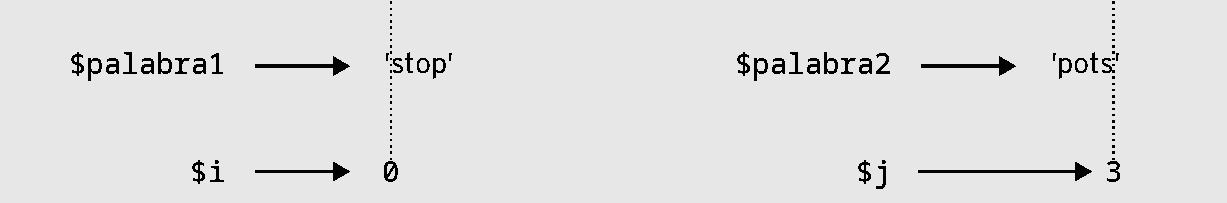
\includegraphics[scale=0.5]{figs/state6.pdf}}
\caption{Diagrama de estado.}
\label{fig.state4}
\end{figure}

Tomamos ciertas libertades para acomodar las variables en
el cuadro y agregar líneas punteadas para mostrar que los valores de
{\tt \$i} y {\tt \$j} indican caracteres en {\tt \$palabra1} y
{\tt \$palabra2}.

Comienza con este diagrama, ejecuta el programa en papel, 
cambia los valores de {\tt \$i} y {\tt \$j} durante cada iteración.
Encuentra y arregla el segundo error en esta función.

Solución: \ref{sol_isreverse}.
\label{isreverse}
\index{is-reverse}


\section{Glosario}

\begin{description}

\item[Objecto] Algo que una variable puede almacenar. 
Por el momento, puedes usar ``objeto`` y ``valor`` indistintamente.
\index{object}

\item[Secuencia] Una colección ordenada de valores donde cada valor
es identificado por un índice entero.
\index{sequence}

\item[Artículo] Uno de los valores en una secuencia.
\index{item}

\item[Índice] Un valor entero que se usa para seleccionar un
artículo en una secuencia, tal como un carácter en un cadena 
de texto. En Perl, los índices comienzan desde el 0.
\index{index}

\item[Rebanada] Una parte de una cadena de texto especificada por un
rango de índices.
\index{slice}

\item[Cadena de texto vacía] Una cadena de texto sin caracteres y con longitud 0,
representada por dos comillas.
\index{empty string}

\item[Recorrer] Iterar a través de los artículos de una secuencia,
realizando una operación similar en cada uno de ellos.
\index{traversal}

\index{search}
\item[Búsqueda] Una patrón de recorrido que para cuando encuentra
lo que está buscando.
\index{search!pattern}
\index{pattern!search}

\index{counter}
\item[Contador] Una variable que se usa para contar algo, usualmente
inicializada a cero y posteriormente incrementada.

\index{regular expression}
\item[Expresiones  regulares] Un sublenguaje de computación
derivado de la teoría de lenguajes formales.

\index{pattern}
\item[Patrón] Una secuencia de caracteres con sintaxis especial
que describen de izquierda a derecha el contenido que se intenta
coincidir dentro de una cadena de texto en particular.

\index{regex}
\item[Regexes] Un sublenguaje de coincidencia de patrón de Perl~6
derivado de las expresiones regulares.

\index{backtracking}
\item[Vuelta atrás] El proceso por el cual,
dado un intento de coincidencia fallido en una cadena de texto, el motor de regex 
abandona parte del intento de coincidencia actual, vuelve atrás
en la cadena de texto, e intenta nuevamente para ver si puede
encontrar una nueva ruta a una coincidencia exitosa. 
El proceso de vuelta atrás eventualmente para tan pronto una
coincidencia exitosa ocurre, o finalmente cuando todas las 
coincidencias posibles fallan. Este proceso se conoce como
\emph{backtracking} en inglés.

\end{description}


\section{Ejercicios}


\begin{exercise}
\label{count_a}
\index{count method}
\index{method!count}
\index{index function}

Escribe una subrutina que use la función {\tt index}  en un bucle
para contar el número de caracteres ``a`` en \verb|`banana`| como 
hicimos en la Sección~\ref{counter}. Modifícala para contar
cualquier letra en cualquier palabra pasadas como argumentos 
a la subrutina.

Escribe otra subrutina para contar una letra dada en una 
palabra dada usando la función {\tt substr}.
\index{substr function}

Solución: \ref{sol_count_a}
\end{exercise}


\begin{exercise}

\label{islower}
\index{lower case!character class}
\index{character class}
La categoría de caracteres \verb|<[a..z]>| coinciden con cualquier
carácter en minúscula (solo caracteres ASCII en minúscula, no caracteres
Unicode). La siguiente subrutina:

\begin{lstlisting}
sub es-minúscula (Str $char) { 
    return so $char ~~ /^<[a..z]>$/
}
\end{lstlisting}

debería devolver {\tt True} si su argumento es una letra ASCII
en minúscula y de lo contrario, {\tt False}. Asegúrate de que 
funcione como se espera (y arréglala si es necesario). La 
función {\tt so} coacciona el resultado de la coincidencia de regex 
en un valor Booleano.

Las siguientes subrutinas usan la subrutina {\tt es-minúscula}
y su trabajo es chequear si una cadena de texto contiene 
letras en minúsculas, pero algunas de ellas no funcionan 
adecuadamente. Analiza cada subrutina manualmente, 
determina si funciona bien, y describe lo que actualmente
hace (puedes asumir que el parámetro es una cadena de texto).
Después, pruébalas todas con varias cadenas de texto para chequear
si tu análisis estaba en lo cierto.

\begin{lstlisting}
# ADVERTENCIA: algunas de las siguientes subrutinas
#              no funcionan correctamente.

sub cualquier_minúscula1(Str $cadena){
    for $cadena.comb -> $char {
        if es-minúscula $char {
            return True;
        } else {
            return False;
        }
    }
}

sub cualquier_minúscula2(Str $cadena){
    for $cadena.comb -> $char {
        if es-minúscula "char" {
            return True;
        } else {
            return False;
        }
    }
}

sub cualquier_minúscula3(Str $cadena){
    my $flag;
    for $cadena.comb -> $char {
        $flag =  es-minúscula $char;
    }
    return $flag;
}

sub cualquier_minúscula4(Str $cadena){
    my $bandera = False;
    for $cadena.comb -> $char {
        $bandera = $bandera or es-minúscula $char;
    }
    return $bandera;
}

sub cualquier_minúscula5(Str $cadena){
    my $flag = False;
    for $cadena.comb -> $char {
        if es-minúscula $char {
            $flag = True;
        }
    }
    return $flag;
}

sub cualquier_minúscula6(Str $cadena){
    for $cadena.comb -> $char {
        if es-minúscula $char {
            return 'True';
        }
    }
    return 'False';
}

sub cualquier_minúscula7(Str $cadena){
    for $cadena.comb -> $char {
        return True if es-minúscula $char;
    }
    return False;
}

sub cualquier_minúscula8(Str $cadena){
    for $cadena.comb -> $char {
        return False unless es-minúscula $char;
    }
    return True;
}

sub cualquier_minúscula9(Str $cadena){
    for $cadena.comb -> $char {
        if not es-minúscula $char {
            return False;
        }
    return True;
    }
}
\end{lstlisting}

Solución: \ref{sol_islower}.

\end{exercise}


\begin{exercise}
\index{letter rotation}
\index{rotation, letter}
\index{Caesar cipher}

\label{rotate}
Un cifrado César es una forma débil de cifrado que involucra
la ``rotación`` de cada letra por un número fijo de posiciones.
La rotación de una letra se refiere a su desplazamiento a través
del alfabeto, y puede envolverse alrededor si es necesario, 
así que ``A`` rotada por 3 corresponde a ``D`` y ``Z`` rotada por
1 corresponde a ``A``.

Para rotar una palabra, rota cada letra por el mismo número de posiciones.
For ejemplo, ``educar`` rotada por 7 es ``lkbjhy`` y ``carta`` rotada por 
-10  es ``sqhjq``. (Para el cifrado, usamos solo caracteres del alfabeto
básico latino ISO.) En la película
{\em 2001: A Space Odyssey}, la computadora de la nave se llama 
HAL, que es una rotación de IBM por -1.

Escribe una función llamada \verb|rotar-palabra| que toma una cadena de texto
y un número entero como parámetros, y devuelve una nueva cadena que 
contiene las letras de la cadena original rotadas por el monto dado.


Podrías querer utilizar las funciones integradas {\tt ord}, 
la cual convierte un carácter a su código numérico (Unicode code point),
y {\tt char}, la cual convierte tales código numérico devuelta los
caracteres:
\index{ord function}
\index{chr function}
\index{function!ord}
\index{function!chr}

\begin{lstlisting}
> say 'c'.ord;
99
> say chr 99
c
\end{lstlisting}
%

Las letras del alfabeto están codificadas en orden 
alfabético, así que por ejemplo:
\index{alphabetic order}

\begin{lstlisting}
> ord('c') - ord('a')
2
\end{lstlisting}

dado que \verb|'c'| es la segunda letra después de \verb|'a'|
en el alfabeto. Pero ten pendiente: los códigos numéricos para
las letras mayúsculas son diferentes.
\index{upper case}
\index{case!upper}

\index{rot13}
Bromas en la Internet que tienen el potencial de ser ofensivas
son algunas veces codificadas en ROT13, el cual es un cifrado 
César con rotación 13. Dado que 13 es la mitad del número de letras
en nuestro alfabeto, la aplicación de una rotación por 13 devuelve la
palabra original, así que el mismo procedimiento puede usarse
para cifrar y descifrar en rotación 13. Si no te ofendes fácilmente,
encuentra y descifra algunas de estas bromas. (ROT13 se usa también 
para otros propósitos, tales como ocultar débilmente la solución de
un acertijo.)

Solución: \ref{sol_rotate}.

\end{exercise}




\chapter{Caso Práctico: Juego de Palabras}
\label{wordplay}

En lugar de introducir conceptos nuevos, el propósito de 
este capítulo es dejarte practicar y consolidar el conocimiento
que has adquirido hasta ahora. Para ayudarte a ganar experiencia
con la programación, discutiremos un caso práctico que involucra
la solución de sopas de palabras al buscar palabras que tienen
ciertas propiedades. Por ejemplo, encontraremos los palíndromos
más largos en inglés y buscaremos palabras cuyas letras aparecen
en orden alfabético. Y presentaré otro plan de desarrollo de programa:
reducción a un programa previamente solucionado.

\section{Lectura de y Escritura a un Archivo}

Para los ejercicios en este capítulos, necesitaremos que nuestros
programas lean texto desde los archivos. En muchos lenguajes 
de programación, usualmente esto significa que necesitamos una sentencia
que abra un archivo, después una sentencia o grupo de sentencias 
para leer el contenido del archivo, y finalmente una sentencia para
cerrar el archivo (aunque esta operación puede realizarse automáticamente
en algunas circunstancias).
\index{file!reading from}
\index{file!writing to}
\index{file!open statement}
\index{file!close statement}

Aquí estamos interesados en archivos de texto que están compuestos 
por líneas separadas por caracteres lógicos de nueva línea; 
dependiendo de tu sistema operativo, lógicos caracteres de nueva línea
consisten de uno (Linux, Mac) o dos (Windows) caracteres físicos (bytes).
\index{newline character}

La función integrada de Perl {\tt open} toma la ruta (\emph{path} en inglés) la cual indica donde el 
archivo se encuentra y el nombre del archivo. {\tt open} devuelve
un {\bf descriptor de archivo} ({\tt IO::Handle object}) que puedes usar
para leer (o para escribir) del mismo):
\index{open function}
\index{function!open}
\index{plain text}
\index{text!plain}
\index{object!file}
\index{file handle}
\index{function!slurp-rest}

\begin{verbatim}
my $fh = open("ruta/a/mi_archivo.txt", :r);
my $datos = $fh.slurp-rest;
$fh.close;
\end{verbatim}
%
La opción {\tt :r}  ({\tt read}) es el modo de escritura. {\tt \$fh} es
un nombre común para un descriptor de archivo ({\bf f}ile {\bf h}andle en inglés).
El \emph{objeto de archivo} provee métodos para leer, tales como {\tt slurp-rest}
el cual devuelve el contenido completo del archivo desde la posición actual hasta
el final (y el contenido completo del archivo lo hemos abierto por primera vez).

Esta es la manera tradicional de abrir y leer archivos en la mayoría de
los lenguajes.
\index{read mode}
\index{file mode!read}

No obstante, el rol {\tt IO} de Perl (en términos simples, un rol 
es una colección de métodos relacionados) ofrece métodos más simples
los cuales pueden abrir y leerlo en una sola instrucción (i.e., 
sin tener que primero abrir un descriptor de archivo y después cerrarlo):
\index{role}
\index{IO role}

\begin{verbatim}
my $texto = slurp "ruta/a/mi_archivo.txt";
# alternativamente:
my $texto = "ruta/a/mi_archivo.txt".IO.slurp;
\end{verbatim}
%

\index{slurp function}
{\tt slurp} toma la responsabilidad de abrir y cerrar el
archivo por ti.

Podemos también leer el archivo línea por línea, lo cual es 
mu práctico si cada línea contiene una entidad lógica tal como
un registro, y es especialmente útil para archivos muy grandes
que podrían no caber en la memoria:

\begin{verbatim}
for 'ruta/a/mi_archivo.txt'.IO.lines -> $línea {
    # Haz algo con la $línea
}
\end{verbatim}
%
Por defecto, el método {\tt .lines} removerá el caracteres de nueva línea
colgantes de cada línea, para que no tengas que preocuparte sobre ellos.
\index{IO.lines method}
\index{IO.slurp method}
\index{slurp function}
%

No hemos estudiados los arrays aún, pero puedes también leer
todas las líneas de un archivo en un array, con cada línea del
archivo volviéndose un artículo del array. Por ejemplo, puedes
cargar el archivo {\em mi\_archivo.txt} en el array \verb|@líneas|:
\index{array}

\begin{verbatim}
my @líneas = "mi_archivo.txt".IO.lines;
\end{verbatim}
%

El acceso a cada línea puede entonces hacerse con el operador bracket
y un índice. Por ejemplo, para imprimir la primera y séptima línea:

\begin{verbatim}
say @líneas[0];
say @líneas[6];
\end{verbatim}
%
Para escribir datos en un archivo, es posible abrirlo al igual 
que cuando queremos leer desde el mismo, excepto que la opción
{\tt :w} (write) (\emph{escritura}) debe usarse:
\index{write mode}
\index{file mode!write}

\begin{verbatim}
my $fh = open("ruta/a/mi_archivo.txt", :w);
$fh.say("escribir esta línea en el archivo");
$fh.close;
\end{verbatim}

Sé cuidadoso con esto. Si el archivo ya existía, cualquier
contenido será sobrescrito. Así que sé cauteloso al abrir un archivo
en el modo de escritura, debido a que podrías borrar todo el 
contenido de un archivo si no tienes cuidado. 

También es posible abrir el archivo en modo de concatenación, usando
la opción {\tt :a} (append). Con esta opción, los datos nuevos serán 
entonces agregados al contenido existente.
\index{append mode}
\index{file mode!append}

La escritura a un archivo puede simplificarse con el uso de la función
{\tt spurt}, la cual abre el archivo, escribe los datos en el mismo, y
consecuentemente cierra:
\index{spurt function}

\begin{verbatim}
spurt "ruta/a/mi_archivo.txt", "escribir esta línea en el archivo\n";
\end{verbatim}

Usado de esta manera, {\tt spurt} sobrescribirá cualquier contenido existente
en el archivo. También puede usarse en el modo de concatenación con la 
opción {\tt :append}:
\index{spurt function!append mode}

\begin{verbatim}
spurt "ruta/a/mi_archivo.txt", "escribir esta línea en el archivo\n ", :append;
\end{verbatim}


\section{Lectura de Listas de Palabras}
\label{wordlist}

Para los ejercicios en este capítulo necesitamos una lista de palabras
en español. Hay muchas listas de palabras en la web, pero una de la
más adecuada para nuestro propósito es una de las listas de palabras
coleccionada y cedida al dominio público por Grady Ward como parte
del proyecto léxico Moby (ver \url{http://wikipedia.org/wiki/Moby_Project}).
Es una lista de 113,809 palabras oficiales de crucigramas; es decir, 
palabras que son consideradas válidas en un crucigrama y otros juegos de
palabras. En la colección Moby, el nombre del archivo es \emph{spanish.txt};
puedes descargar una copia
desde \url{https://www.gutenberg.org/files/3206/files/spanish.txt}.
\index{Moby Project}
\index{crosswords}
\index{word list}

\begin{description}
\item {\bf Nota del traductor}: En lugar de utilizar la lista de palabras en \emph{spanish.txt}
del proyecto Moby, he decidido utilizar la lista en \emph{lemario.txt} (\url{https://gitlab.com/uzluisf/piensaperl6/tree/master/suplementos/lemario.txt}) 
que contiene aproximadamente 88,000 palabras\footnote{
También puedes encontrar el lemario y más información sobre el mismo aquí: (\url{http://olea.org/proyectos/lemarios/index.html})}. La decisión se debe a que la lista de 
palabras en español del proyecto Moby contiene muchas palabras que no están
formateadas apropiadamente. 
\end{description}

Este archivo contiene texto simple (con cada palabra de la lista
en su propia línea), así que puedes abrirlo con un editor de texto,
pero también puedes leerlo con Perl. Hagamos esto en el modo
interactivo (con el REPL):
\index{interactive mode}
\index{REPL}

\begin{verbatim}
> my $fh = open("lemario.txt", :r);
IO::Handle<lemario.txt>(opened, at octet 0)
> my $línea = get $fh;
aa
> say "<<$línea>>";
<<aa>>
\end{verbatim}

La función {\tt get} lee una línea del descriptor de archivo.
\index{get function}

La primera palabra en esta lista en particular es ``a``.

Imprimir la variable \verb|$línea| entre los paréntesis angulares
dentro de una cadena de texto nos muestra que la función {\tt get}
removió explícitamente los caracteres de nueva línea colgantes, en este
caso una combinación de los caracteres \verb|\r\n| (un retorno de carro
 y una nueva línea), dado que este archivo aparentemente fue preparado en Windows.

El descriptor de archivo mantiene un registro de lo que se ha leído
desde el archivo y lo que debe leerse después, así que se llamas
a {\tt get} otra vez, obtienes la siguiente línea:

\begin{verbatim}
> my $línea = get $fh;
a-
\end{verbatim}
%
La palabra siguiente es ``a-''. Si llamas a {\tt get} nuevamente,
obtienes la palabra ``aarónico``. 

Esto es grandioso si queremos explorar las primeras líneas del
archivo {\tt lemario.txt}, pero no vamos a explorar las casi 
88,000 líneas del archivo de esta forma.

Necesitamos que un bucle lo haga por nosotros. Podríamos insertar
la nueva instrucción {\tt get} en un bucle {\tt while}, pero
hemos visto una manera más fácil y más eficiente de hacerlo con
un bucle {\tt for} y el método {\tt IO.lines}, sin la inconveniencia
de abrir o cerrar el archivo:
\index{for loop}
\index{IO.lines method}

\begin{verbatim}
for 'lemario.txt'.IO.lines -> $línea {
    say $línea;
}
\end{verbatim}
%
Este código lee el archivo línea por línea, e imprime cada línea
en la pantalla. Pronto haremos cosas más interesantes que solo
mostrar las líneas en la pantalla.

\section{Ejercicios}

Este caso práctico consiste principalmente de ejercicios y soluciones
dentro del cuerpo del capítulo porque solucionar los ejercicios es la
manera principal de enseñar el material de este capítulo. Por lo tanto, 
las soluciones a estos ejercicios se encuentran en las siguientes 
secciones de este capítulo, no en el apéndice. Por lo menos 
deberías tratar de solucionar cada uno de ellos antes de leer las
soluciones.

\begin{exercise}
Escribe un programa que lee el archivo {\tt lemario.txt} e imprime
solo las palabras con más de 20 caracteres.
\index{whitespace}

\end{exercise}

\begin{exercise}

En 1939, Ernest Vincent Wright publicó una novela con aproximadamente
50,000 palabras llamada {\em Gadsby} que no contiene la letra ``e``. 
Dado que ``e`` es la letra más común en inglés, eso no es fácil
de hacer. De hecho, es difícil construir un solo pensamiento sin
usar la letra más común. Tal escritos donde se omite alguna letra
es algunas veces conocido como un lipograma.
\index{Wright, Ernest Vincent}
\index{Gadsby}
\index{lipogram}

Escribe una subrutina llamada \verb|sin-e| que devuelve {\tt True}
si la palabra dada no contiene la letra ``e``.
\label{no_e}

Modifica tu programa del ejercicio previo para imprimir solamente
palabras que no tienen ``e`` y calcular el porcentaje de palabras
en la lista que no tienen ``e``.

(El diccionario de palabras que estamos usando, \emph{lemario.txt}, 
tiene completamente en letras minúsculas, así que no tienes que preocuparte
acerca de la ``E`` mayúscula.)


\end{exercise}


\begin{exercise} 

Escribe una subrutina llamada {\tt evitar} que toma una palabra
y una cadena de texto de letras prohibidas, y devuelve {\tt True}
si la palabra no contiene ninguna de las letras prohibidas.

Después, modifica tu programa para encitar el usuario a entrar
una cadena de texto de letras prohibidas y después imprimir el número
de palabras que no contienen ningunas de ellas. ?`Puedes encontrar una
combinación de cinco letras prohibidas que excluya  el menor número
de palabras?
\end{exercise}



\begin{exercise}

Escribe una subrutina llamada \verb|usa-solamente| que toma una palabra
y una cadena de letras, y devuelve {\tt True} si la palabra contiene
solo las letras en la lista. ?`Puedes construir una oración usando solo
las letras {\tt acefhlo}?  
%Other than ``Hoe alfalfa?''

\end{exercise}


\begin{exercise} 

Escribe una subrutina llamada \verb|usa-todas| que toma una palabra
y una cadena de letras requeridas, y devuelve {\tt True} si la palabra
usa todas las letras requeridas por lo menos una vez. ?`Cuántas 
palabras se encuentran ahí que usan todas las vocales {\tt aeiou}? 
?`Y cuántas usan {\tt aeiouy}?

\end{exercise}


\begin{exercise}

Escribe una función llamada \verb|es_abecedaria| que devuelve
{\tt True} si las letras en una palabra aparecen en orden 
alfabético (letras dobles son aceptables). ?`Cuántas palabras
son abecedarias?

\index{abecedarian}

\end{exercise}



\section{Búsqueda}
\label{search}
\index{search!pattern}
\index{pattern!search}
\index{regex}

La mayoría de los ejercicios en la sección previa tiene algo en
común; pueden solucionarse con el patrón de búsqueda (y la función
{\tt index} que vimos en la Sección~\ref{find} 
(p.~\pageref{find}). Muchos de ellos también pueden solucionarse
con regexes.

\subsection{Palabras con Más de 20 Caracteres (Solución)}

La solución al ejercicio más simple ---imprimir todas las palabras
de {\tt lemario.txt} que tienen más de 20 caracteres--- es:

\begin{verbatim}
for 'lemario.txt'.IO.lines -> $línea {
    say $línea if $línea.chars > 20
}
\end{verbatim}
%

Dado que el código es tan simple, esto es un ejemplo típico
de un one-liner útil (como se describió en la 
Sección~\ref{one-liner mode}). Asumiendo que quieras saber las
palabras con más de 20 caracteres, no necesitas ni siquiera escribir
un script, guardarlo y ejecutarlo. Simplemente puedes teclear esto
en la prompt de tu sistema operativo:
\label{one-liner-example}
\index{one-liner mode}

\begin{verbatim}
$ perl6 -n -e '$_.say if $_.chars > 20;' lemario.txt
\end{verbatim} 
%
La opción ``-e`` le dice a Perl que el script a ser ejecutado
viene en la línea de comando entre comillas. La ``-n`` le indica
a Perl que lea el archivo línea por línea después de la línea
de comando, almacene cada línea en la variable tópico \verb|$_|,
y aplique el contenido del script a cada línea. Y el script en modo
one-liner solo imprime el contenido de \verb|$_| si su longitud
es mayor que 20.
\index{topical variable}

Para simplificarlo un poco, las dos opciones \verb|-n| y \verb|-e|
pueden agruparse como \verb|perl6 -ne|. En adición, la variable tópico
\verb|$_| puede omitirse en las llamadas de método (en otras palabras,
si un método no tiene invocante, el invocante será \verb|$_| por defecto).
Finalmente, el punto y coma colgante puede igualmente removerse.
El script en modo one-liner más arriba puede entonces simplificarse
aún más:
\index{invocant}

\begin{verbatim}
$ perl6 -ne '.say if .chars > 20' lemario.txt
\end{verbatim} 
%
Recuerda que, si está intentando esto en Windows, necesita reemplazar las 
comillas simples con las comillas dobles (y viceversa si el script
contiene comillas dobles):

\begin{verbatim}
C:\Users\Laurent>perl6 -ne ".say if .chars > 20" lemario.txt
\end{verbatim} 
%

\subsection{Palabras Sin ``e'' (Solución)}

Una subrutina que devuelve {\tt True} para palabras que no tienen ``e''
(Ejercicio~\ref{no_e}) es igualmente simple:

\begin{verbatim}
sub sin-e (Str $palabra) {
    return True unless defined index $palabra, "e";
    return False;
}
\end{verbatim}
%

La subrutina simplemente devuelve {\tt True} si la función {\tt index} 
no encontró una ``e`` en la palabra recibida como un parámetro y
por lo contrario, devuelve {\tt False}.

Nota que esto funciona correctamente porque la lista de palabras usada
(\emph{lemario.txt}) está completamente en letras minúsculas. La subrutina
más arriba necesitaría ser modificada si fuera a ser llamada con palabras
que contienen letras mayúsculas.

Dado que la función {\tt defined} devuelve un valor Booleano, podríamos 
simplificar nuestra subrutina:
\begin{verbatim}
sub sin-e (Str $palabra) {
    not defined index $palabra, "e";
}
\end{verbatim}
%

Podríamos también haber usado un regex para comprobar la 
presencia de una ``e`` en la segunda línea de esta subrutina:

\begin{verbatim}
    return True unless $palabra ~~ /e/;
\end{verbatim}
%

Esta sintaxis bastante concisa es atractiva, pero cuando se
busca por una coincidencia literal exacta, la función {\tt index}
es probablemente más eficiente (más rápida) que un regex.

Buscar y contar las palabras sin ``e`` en nuestra lista de palabras 
no es muy difícil:

\begin{verbatim}
sub sin-e (Str $palabra) {
    not defined index $palabra, "e";
}

my $cuenta-total = 0;
my $cuenta-sin-e = 0;
for 'lemario.txt'.IO.lines -> $línea { 
    $cuenta-total++;
    if sin-e $línea {
        $cuenta-sin-e++;
        say $línea;
    }
}
say "=" x 24;
say "Cuenta total de palabras: $cuenta-total";
say "Palabras sin 'e': $cuenta-sin-e";
printf "Porcentaje de palabras sin 'e': %.2f %%\n", 
        100 * $cuenta-sin-e / $cuenta-total;
\end{verbatim}

El programa anterior mostrará lo siguiente al final de 
su salida:

\begin{verbatim}
========================
Cuenta total de palabras: 87899
Palabras sin 'e': 36671
Porcentaje de palabras sin 'e': 41.72 %
\end{verbatim}

Así que más de un tercio de las palabras en nuestra lista no
tienen ``e``.

\subsection{Evitar Otras Letras (Solución)}

\index{generalization}
La subrutina {\tt evitar} es una versión más general de 
\verb|sin-e|, pero tiene la misma estructura:

\begin{verbatim}
sub evitar (Str $palabra, Str $prohibida) {
    for 0..$prohibida.chars - 1 -> $idx {
        my $letra = substr $prohibida, $idx, 1;
        return False if defined index $palabra, $letra;
    }
    True;
}

\end{verbatim}
%
Podemos devolver {\tt False} tan pronto encontremos una letra
prohibida; si llegamos al final del bucle, devolvemos {\tt True}.
Debido a que una subrutina devuelve la última expresión evaluada,
no necesitamos usa la sentencia {\tt return True} explícitamente
en la última línea de código más arriba. He usado esta característica
como un ejemplo; podrías encontrarlo más claro {\tt devolver} los valores 
explícitamente, excepto quizás con subrutinas de una línea muy simples.

Nota que tenemos dos bucles anidados implícitamente. Podríamos 
invertir los bucles externo e interno:

\begin{verbatim}
sub evitar(Str $palabra, Str $prohibida) {
    for 0..$palabra.chars - 1 -> $idx {
        my $letra = substr $palabra, $idx, 1;
        return False if defined index $prohibida, $letra;
    }
    True;
}
\end{verbatim}
%

El código principal que llama la subrutina más arriba es similar
al código que llama a {\tt sin-e} y podría lucir así:

\begin{verbatim}
my $cuenta-total = 0;
my $cuenta-no-prohibidas = 0;

for 'lemario.txt'.IO.lines -> $línea { 
    $cuenta-total++;
    $cuenta-no-prohibidas++ if evitar $línea, "eiou";
}

say "=" x 24;
say "Cuenta total de palabras: $cuenta-total";
say "Palabras sin letras prohibidas: $cuenta-no-prohibidas";
printf "Percentaje de palabras sin letras prohibidas: %.2f %%\n", 
        100 * $cuenta-no-prohibidas / $cuenta-total;
\end{verbatim}    
%
  

\subsection{Usando Solo Algunas Letras (Solución)}

\verb"usa-solamente" es similar a nuestra subrutina {\tt evitar} 
excepto que el sentido de la condición está invertido:

\begin{verbatim}
sub usa-solamente(Str $palabra, Str $disponible) {
    for 0..$palabra.chars - 1 -> $idx {
        my $letra = substr $palabra, $idx, 1;
        return False unless defined index $disponible, $letra;
    }
    True;
}
\end{verbatim}
%
En lugar de una lista de letras prohibidas, tenemos una lista
de letras disponibles. Si encontramos una letra en {\tt \$palabra}
que no está en {\tt \$disponible}, podemos devolver {\tt False}. 
Y devolvemos {\tt True} si llegamos al final del bucle.

\subsection{Usando Todas las Letras de una Lista (Solución)}

\verb"usa-todas" es similar a las subrutinas previas,
excepto que invertimos el rol de la palabra y la cadena 
de letras:

\begin{verbatim}
sub usa-todas(Str $palabra, Str $requerida) {
    for 0..$requerida.chars - 1 -> $idx {
        my $letra = substr $palabra, $idx, 1;
        return False unless defined index $palabra, $letra;
    }
    return True;
}
\end{verbatim}
%
En lugar de recorrer las letras en {\tt \$palabra}, el bucle
recorre las letras requeridas. Si cualquiera de las letras
requeridas no aparece en la palabra, podemos devolver {\tt False}.
\index{traversal}

Si estabas realmente pensando como un científico de la computación, 
habrías reconocido que \verb|usa-todas| era una instancia de un
problema previamente resuelto en inverso: si la palabra~A usas todas
las letras de la palabra~B,  entonces la palabra~B usa solo las letras
de la palabra~A. Así que podemos llamar la subrutina {\tt usa-solamente}
y escribir:

\begin{verbatim}
sub usa-toda ($palabra, $requerida) {
    return usa-solamente $requerida, $palabra;
}
\end{verbatim}
%
Este es un ejemplo de un plan de desarrollo de programa conocido como
{\bf reducción a un problema previamente solucionado}, lo cual 
significa que reconoces el problema con el cual estás trabajando
como una instancia de un problema ya solucionado y aplica una
solución ya existente. 
\index{reduction to a previously solved problem} 
\index{development plan!reduction}

\subsection{Orden Alfabético (Solución)}

Para \verb|es_abecedaria| tenemos que comparar las letras adyacentes.
Cada vez en nuestro bucle {\tt for}, definimos una letra como nuestra
letra actual y la comparamos con la anterior:

\begin{verbatim}
sub es_abecedaria ($palabra) {
    for 1..$palabra.chars - 1 -> $idx {    
        my $letra-actual = substr $palabra, $idx, 1;
        return False if $letra-actual lt substr $palabra, $idx - 1, 1;  
    }     
    return True
}
\end{verbatim}

Una alternativa es usar recursión:
\index{recursion}

\begin{verbatim}
sub es-abecedaria (Str $palabra) {
    return True if $palabra.chars <= 1;
    return False if substr($palabra, 0, 1) gt substr($palabra, 1, 1);
    return es-abecedaria substr $palabra, 1;
}
\end{verbatim}

Otra opción es usar bucle {\tt while}:

\begin{verbatim}
sub palabra(Str $palabra):
    my $i = 0;
    while $i < $palabra.chars -1 {
        if substr($palabra, $i, 1) gt substr ($palabra, $i+1, 1) {
            return False;
        }
        $i++;
    }
    return True;
}
\end{verbatim}
%
El bucle comienza con {\tt \$i=0} y termina con {\tt i=\$palabra.chars -1}.
Cada vez a través del bucle, se compara el carácter $i$th (el cual puedes
considerar como el carácter actual) al carácter $i+1$th (el cual puedes
considerar como el carácter siguiente).

Si el carácter siguiente es menor (alfabéticamente posterior) que el 
carácter actual, entonces hemos descubierto una falla en la tendencia
del abecedario, y devolvemos {\tt False}.

Si llegamos al final del bucle sin encontrar una falla, entonces
la palabra pasa la prueba. Para convencerte que el bucle finaliza
correctamente, considera un ejemplo como \verb|'flossy'|. La
longitud de la palabra es 6, así que la última vez que el bucle 
se ejecuta es cuando \verb|$i| es 4, el cual es el índice del
penúltimo carácter. En la última iteración, se compara el penúltimo
carácter (la segunda ``s'') al último (la ``y''), que es lo
deseamos.
\subsection{Otro Ejemplo de Reducción a un Problema Previamente Solucionado}

\index{palindrome}
\label{palindrome_2}

Aquí tenemos una versión de \verb|es_palindromo|(ver Ejercicio~\ref{palindrome})
que usa dos índices; uno comienza al inicio e incrementa, mientra que el
otro comienza al final y disminuye:

\begin{verbatim}
sub un-car (Str $cadena, $idx) {
    return substr $cadena, $idx, 1;
}
sub es-palindromo (Str $palabra) {
    my $i = 0;
    my $j = $palabra.chars - 1;

    while $i < $j {
        return False if un-car($palabra, $i) ne 
                        un-car($palabra, $j);
        $i++;
        $j--;
    }
    return True;
}
\end{verbatim}

O podríamos reducirlo a un problema previamente solucionado
y escribir:
\index{reduction to a previously solved problem}
\index{development plan!reduction}

\begin{verbatim}
sub es-palindromo (Str $palabra) {
    return es-inversa($palabra, $palabra)
}
\end{verbatim}
%
usando \verb|es-inversa| de la Sección~\ref{isreverse} (
pero deberías probablemente elegir la versión corregida de la
subrutina \verb|es-inversa| dada en el apéndice: 
ver Subsección~\ref{sol_isreverse}).


\section{Depuración de Programas}
\index{debugging}
\index{testing!is hard}
\index{program!testing}

Hacer pruebas manuales de los programas es difícil. Las funciones en este
capítulo son relativamente fáciles para probar porque puedes chequear 
el resultado manualmente. Aún así, es algo entre difícil e imposible elegir
un conjunto de palabras que prueben para todos los errores posibles.

Por ejemplo, tomemos el caso de la subrutina \verb|sin-e|. En esta función, hay dos casos
que debemos chequera: palabras que tienen una ``e`` debería devolver {\tt False},
y palabras que no tienen ninguna ``e`` deberían devolver {\tt True}. Esto
no representa problema alguno debido a que es fácil encontrar palabras
que representan cada caso.

Dentro de cada caso, existen casos que son menos obvios. Entre las palabras
que tienen una ```e``, deberías probar palabras con una ``e`` al inicio, 
al final, y en el medio. Deberías probar con palabras largas, palabras cortas
y con palabras muy cortas, como una cadena de texto vacía. La cadena de texto 
vacía es un ejemplo de un {\bf caso especial}, el cual es uno de los 
casos que no son obvios donde los errores usualmente merodean.
\index{special case}

Además de las pruebas de casos que generes, puedes también someter
tu programa a una prueba con una lista de palabras como \emph{lemario.txt}.
Al escanear la salida, podrías atrapar errores, pero debes ser cuidadoso:
podrías atrapar un tipo de error (palabras que no deberían ser incluidas,
pero son incluidas) y dejar pasar otros errores (palabras que deberían ser
incluidas pero no son incluidas).

En general, las pruebas pueden ayudar a encontrar errores, pero no es fácil
generar un buen conjunto de pruebas de casos, y aún si lo haces, no puedes
estar seguro que tu programa es correcto.

Según un legendario científico de la computación:
\index{testing!and absence of bugs}

\begin{quote}
	
La depuración de programas puede usarse para mostrar la presencia
de errores, pero jamás para mostrar la ausencia de los mismos\footnote{
"Program testing can be used to show the presence of bugs, 
but never to show their absence!" --- Edsger W. Dijkstra
}.

--- Edsger W. Dijkstra
\end{quote}
\index{Dijkstra, Edsger}


\section{Glosario}

\begin{description}

\item[Objeto de archivo] Un valor que representa un archivo abierto.
\index{file object}
\index{object!file}

\item[Reducción a un problema previamente solucionado] Una manera de 
solucionar un problema al expresarlo como una instancia de un problema
que fue solucionado previamente.
\index{reduction to a previously solved problem}
\index{development plan!reduction}

\item[Caso especial] Un caso de prueba que es atípico o que no es evidente
(y con pocas posibilidades de ser manejado correctamente). Los términos
\emph{edge case} and \emph{corner case} expresan más o menos la misma
idea.
\index{special case}
\index{edge case}
\index{corner case}

\end{description}


\section{Ejercicios}

\begin{exercise}
\index{Car Talk}
\index{Puzzler}
\index{double letters}
\label{cartalk}

Este pregunta está basada en un Puzzler (acertijo) que fue transmitido en
el programa radial {\em Car Talk} 
(\url{http://www.cartalk.com/content/puzzlers}):

\begin{quote}
Dame una palabra con tres letras dobles consecutivas. Te daré unas
cuantas palabras que casi cualifican, pero no completamente.Por ejemplo,
la palabra committee, c-o-m-m-i-t-t-e-e. Sería un gran ejemplo excepto
por la ``i`` que se escabulle ahí. O Mississippi: M-i-s-s-i-s-s-i-p-p-i.
Si pudieras sacar esas i, sería otro gran ejemplo. No obstante, existe
una palabra que tiene tres pares de letras consecutivas y a mi saber,
esta puede ser la única palabra que satisface dicha condición. 
¡Solo bromeo! Existen probablemente alrededor de 500 de estas palabras pero
solo puede pensar sobre una. ¿Cuál es la palabra?
\end{quote}

Escribe un programa para encontrarla.

Solución: \ref{sol_cartalk}.

\end{exercise}


\begin{exercise}
Aquí presentamos otro Puzzler de{\em Car Talk}
(\url{http://www.cartalk.com/content/puzzlers}):
\label{cartalk2}
\index{Car Talk}
\index{Puzzler}
\index{odometer}
\index{palindrome}

\begin{quote}
``Estaba conduciendo en la autopista el otro día y sucede que
noto mi odómetro. Como la mayoría de odómetros, este
muestra seis dígitos, en millas en números enteros solamente. 
Así que, si mi carro tenía 300,000 millas, por ejemplo, yo 
vería 3-0-0-0-0-0.

Ahora bien, lo que ví ese día fue algo muy interesante. Noté que 
los últimos cuatro dígitos eran palíndromos; es decir, se
pueden leer igual de atrás hacia adelante. Por ejemplo, 5-4-4-5 
es un palíndromo, así que mi odómetro podría leerse 3-1-5-4-4-5.

Una milla más tarde, los últimos 5 números eran palíndromos. Por ejemplo,
podría leerse 3-6-5-4-5-6.  Una milla después de esa, los 4 números
del medio eran palíndromos. ¿Y estás listo para esto? ¡Otra milla más
tarde, todos los 6 números eran palíndromos!``

``La pregunta es, qué había en el odómetro la primera vez que lo miré?''
\end{quote}

Escribe un programa que cheque todos los números de seis dígitos
e imprime cualquier que satisface estos requerimientos.
  
Solución: \ref{sol_cartalk2}.

\end{exercise}


\begin{exercise}
Otro Puzzler de {\em Car Talk} que puedes solucionar con una
búsqueda (\url{http://www.cartalk.com/content/puzzlers}):
\index{Car Talk}
\index{Puzzler}
\index{palindrome}
\label{cartalk3}

\begin{quote}

Recientemente visité a mi madre y me dí cuenta que los dos dígitos
que componen mi edad al ser invertidos resultan en su edad. Por 
ejemplo, si ella tiene 73 años, entonces yo tengo 37. Nos preguntamos
que tan a menudo esto había ocurrido a través de los años pero nos
distraímos con otros temas y jamás obtuvimos una respuesta.

Cuando llegué a la casa fui capaz de deducir que los dígitos de
nuestras edades habían sido reversibles seis veces hasta ahora.
También deducí que si tenemos suerte pasaría nuevamente dentro de
algunos años, y si somos bien suertudos ocurriría una vez más después
de eso. En otras palabras, pasaría 8 veces en total. Así que la pregunta
es, cuál es mi edad ahora?

\end{quote}

Escribe un programa de Perl que busca las soluciones para este Puzzler.
Pista: podrías encontrar el método para el formateo de cadenas de texto
{\tt sprintf} muy útil.
\index{sprintf function}

Solución: \ref{sol_cartalk3}.

\end{exercise}




\chapter{Arrays y Listas}
\label{arrays}

Este capítulo presenta algunos de los tipos integrados
de Perl más útiles, los arrays y las listas.


\section{Las Listas y los Arrays Son Secuencias}
\label{sequence}

Al igual que las cadenas de texto, las {\bf listas} y los {\bf arrays}
son secuencias de valores. En una cadena de texto, los valores son
caracteres; en una lista o en un array, los valores pueden ser
de cualquier tipo. Los valores en una lista o en un array se 
conocen  como {\bf elementos} o algunas veces como {\bf artículos}.
\index{list}
\index{array}
\index{type!list}
\index{type!array}
\index{element}
\index{sequence}
\index{item}

Existen varias diferencias importantes entre las listas y los arrays.
La principal de ellas es que las listas son colecciones ordenadas e inmutables
de elementos: no puedes cambiar el número de elementos en una lista y tampoco puedes
cambiar los elementos individuales tampoco. Los arrays, por el contrario,
son variables y son generalmente mutables: puedes agregar elementos 
a un array, o quizás removerlos. Y también puedes acceder los
elementos individuales de un array y modificarlos. Para que esto sea
posible, los arrays usualmente tienen un nombre (como cualquier otra variable)
aunque algunos arrays son anónimos, lo que significa que no tienen 
un nombre, pero aún tienen otras formas de acceso.

Una lista es también efímera (al menos que se ha asignada a una
variable o algo más): deja de existir tan pronto ha sido usada,
usualmente tan pronto el flujo de ejecución del programa procede
a la siguiente línea de código. Por el contrario, un array tiene
alguna forma de persistencia: tú puedes usarlo en otras partes del
programa si la variable que lo contiene aún está dentro del
ámbito.

Hay varias maneras de crear una lista nueva;
la forma más simple es enumerar sus valores, separados
por comas:
\index{comma operator}
\index{operator!comma}

\begin{lstlisting}
> 3, 4, 5
(3 4 5)
> say (3, 4, 5).WHAT;
(List)
say $_ for 1, 2, 3;
1
2
3
\end{lstlisting}
%

No necesitas usar paréntesis para crear una lista,
pero son usualmente útiles para delimitar los valores,
i.e., para estipular dónde comienza y dónde termina, y
en algunos casos, anular la precedencia.

Ya hemos usado listas en este libro. Si escribimos:

\begin{lstlisting}
> print "$_ " for 1, 3, 5, 9, "\n";
1 3 5 9
 >
> print "$_ " for 1..10;
1 2 3 4 5 6 7 8 9 10 >
\end{lstlisting}

estamos básicamente creando y usando una lista de números
enteros (desde el punto de vista de la jerarquía de tipos en
Perl; esta observación no es totalmente correcta para el segundo
ejemplo, dado que \verb|1..10| es del tipo \emph{Range} y
es transformado en el tipo \emph{Seq}. Sin embargo, esta 
aproximación es suficientemente buena para nuestros 
propósitos aquí).
\index{range!type}
\index{range!operator}

Los arrays son variables cuyo nombre comienzan con
el sigilo \verb|@|. Los arrays con nombres necesitan ser declarados
antes de ser usados, como cualquier otra variable que hemos
visto hasta ahora (excepto la variable tópico, \verb|$_|). 
Una de las formas más fácil de crear un array es asignar una
lista a una variable:
\index{topical variable}
\index{sigil}

\begin{lstlisting}
> my @dígitos_impares = 1, 3, 5, 7, 9;
[1 3 5 7 9]
> say @dígitos_impares.WHAT;
(Array)
> my @números_solo_dígito = 0..9;
[0 1 2 3 4 5 6 7 8 9]
\end{lstlisting}

En el REPL de Perl, un array se muestra entre corchetes
(\verb|[| y \verb|]|), mientras que las listas se muestran
entre paréntesis.
\index{REPL}
\index{square bracket operator}
\index{operator!square bracket}
\index{bracket!square}

Si los elementos no contienen caracteres de espacio, es bien útil
construir una lista (y asignarla a cualquier array si es necesario)
con el operador quote-word \verb|<...>|:
\index{quote-word operator}

\begin{lstlisting}
> my @días-semana = <lun mar mie jue vie>;
[lun mar mie jue vi]
> my @fin-semana = <sab dom>;
[sab dom]
\end{lstlisting}

La ventaja de este método es que no hay necesidad de separar los 
elementos con comas y tampoco hay necesidad de insertar comillas
cuando los elementos son cadenas de texto. Básicamente, el operador
quote-word descompone su contenido por espacios en blanco y devuelve
una lista de palabras, la cual puede ser entonces usada en un bucle
o asignada a un array como en el ejemplo anterior.

La mayoría de este capítulo será dedicado a los arrays. No obstante,
ten presente que muchas de las funciones y operadores de los arrays
que estudiaremos aquí también funcionan con listas (por lo menos
todas aquellas que no violan la propiedad de inmutabilidad de las
listas). 

Los elementos de un array (o una lista) no necesitan ser del mismo
tipo:

\begin{lstlisting}
> my @array-heterogeneo = 1, 2.3, pi, "str", (1, 2, 4);
[1 2.3 3.14159265358979 str (1 2 4)]
\end{lstlisting}

Aquí, el array está compuesto por un entero, 
un racional, un número con coma flotante (tipo {\tt Num}),
una cadena de texto, y  una lista de tres enteros.
Aunque esto podría no ser recomendado por la sanidad mental
del programador quien tendría que usar un array con elementos
tan heterogéneos, Perl no se queja: al final, depende de ti hacer 
sentido de tus datos.

El array anterior hasta contiene una lista de artículos. 
Si iteras sobre los elementos de este array, por ejemplo con
el bucle for, esta lista terminará como un elemento distinto;
este elemento no será ``aplanado`` como tres elementos del
array. Similarmente, {\tt elems} es un método que cuenta el
número de artículos de un array (o de una lista). Al usarlo
en el array anterior produce el siguiente resultado:

\begin{lstlisting}
> say @array-heterogeneo.elems;
5
\end{lstlisting}
%

Como puedes observar, la lista \verb|(1, 2, 4)| cuenta como
un solo elemento en el array.

Una lista dentro de otra es una lista {\bf anidada}.
\index{nested list}
\index{list!nested}

Un array que carece de elementos se conoce
como un array vacío; puedes crear un array vacío con
paréntesis vacíos, \verb|()|:

\begin{lstlisting}
> my @vacío = ();
[]
\end{lstlisting}
\index{empty list}
\index{list!empty}

Este código está realmente asignando una lista vacía al array.
Pero esta sintaxis no es normalmente necesaria para crear un
nuevo array vacío, dado que solo con declarar un array sin 
definirlo tiene el mismo efecto:

\begin{lstlisting}
> my @vacío;
[]
\end{lstlisting}

Así que el uso de paréntesis vacíos (i.e., en la asignación
de una lista vacía) sería necesario para restaurar un
array existente como un array vacío.

\section{Los Arrays Son Mutables}
\label{mutable}
\index{list!element}
\index{access}
\index{index}
\index{subscript}
\index{bracket operator}
\index{operator!bracket}
\index{bracket!square}

\index{index!starting at zero}
\index{coercion}
La sintaxis para acceder los elementos de un array o una lista
usa el operador de corchetes. La expresión dentro de los corchetes
especifica el índice o subíndice, el cual puede ser un 
entero literal (o algún valor que puede ser coaccionado en un 
entero), una variable que contiene un valor numérico,
una lista o un rango de valores numéricos, una expresión o una pieza
de código que devuelve un valor numérico, etc. Comparado con el
comienzo de una array o una lista (de la misma 
manera que los valores devueltos por la función {\tt index}),
los índices comienzan en la posición 0. Así que, el primer elemento
de un array tiene índice 0, el segundo tiene índice 1, etc. Por ejemplo:
\index{zero, index starting at}


\begin{lstlisting}
say <sab dom>[1];             # -> sab (accediendo un elemento de la lista)
my @días-semana = <lun mar mie jue vie>;   # asignando un array
say "El tercer día es @días-semana[2]";    # -> El tercer día es mie
\end{lstlisting}
%

También puedes usar rangos o listas de índices para acceder
partes (o \emph{rebanadas}) de un array o una lista:
\index{slice}
\index{slice!operator}
\index{operator!slice}
\index{index!slice}
\index{list!slice}
\index{slice!list}
\index{range}

\begin{lstlisting}
> my @dígitos-pares = 0, 2, 4, 6, 8;
[0 2 4 6 8]
> my @pequeños-dígitos_pares = @dígitos-pares[0..2];
[0 2 4]
> my @min-max-dígitos-pares = @dígitos-pares[0, 4]
[0 8]
\end{lstlisting}

Si necesitas rebanadas en el orden opuesto, puedes usar
la función {\tt reverse} para revertir el rango:

\begin{lstlisting}
> my @opuestos-pequeños-dígitos_pares = @dígitos-pares[reverse 0..2];
[4 2 0]
\end{lstlisting}

o también puedes revertir los datos que resultan de la expresión
de rebanadas:

\begin{lstlisting}
> my @opuestos-pequeños-dígitos_pares = reverse @dígitos-pares[0..2];
[4 2 0]
\end{lstlisting}

A diferencia de las listas, los arrays son mutables. 
Cuando el operador de corchetes aparece después de un array 
en el lado izquierdo de una asignación, el operador identifica el
elemento del array que será asignado:
\index{mutability}

\begin{lstlisting}
> my @dígitos-pares = 0, 2, 2, 6, 8;   # Oops, error en el segundo 2
[0 2 2 6 8]
> @dígitos-pares[2] = 4; # arreglando el tercer elemento
4
> say @dígitos-pares
[0 2 4 6 8]
\end{lstlisting}
%

El tercer elemento de {\tt \@dígitos-pares}, el cual es (por error) 2,
es ahora 4. Si el índice corresponde a un artículo que no existe aún
en el array, el array se expandaré para incluir el nuevo elemento:

\begin{lstlisting}
> my @impares = 1, 3, 5;
[1 3 5]
> @impares[3] = 7;
7
> say @impares;
[1 3 5 7]
\end{lstlisting}

\index{index!starting at zero}
\index{item assignment}
\index{assignment!item}
\index{reassignment}

\index{elems function or method}
\index{end method}
La función o método {\tt elems} devuelve el número
de elementos de un array. La función o método {\tt end}
devuelve el índice del último elemento de un array:

\begin{lstlisting}
my @nums = 1..5;      # -> [1 2 3 4 5]
say @nums.elems;      # -> 5
say elems @nums;      # -> 5
say @nums.end;        # -> 4
\end{lstlisting}

El método {\tt end} devuelve el resultado del método 
{\tt elems} menos uno porque, dado que los índices comienzan
en la posición 0, el índice del último elemento es igual
al número de elementos menos uno.
\index{zero, index starting at}

La función o método {\tt unique} devuelve una secuencia
de elementos únicos en la lista de entrada o el array (
i.e., el método devuelve la lista original si no hay valores
duplicados):
\index{unique function}
\index{function!unique}

\begin{lstlisting}
> say < a b d c a f d g>.unique;
(a b d c f g)
\end{lstlisting}

Si sabes que la entrada está ordenada (y que, por lo tanto,
los duplicados son adyacentes), en vez de usar la función
{\tt unique}, usa la función {\tt squish} debido a que termina
siendo más eficiente. La función {\tt squish} remueve elementos
duplicados y adyacentes.
\index{squish function}
\index{function!squish}

Para saber si dos arrays son idénticos (estructuralmente 
los mismos, con el mismo tipo y los mismos valores), usa 
el operador de equivalencia {\tt eqv}. Para saber si los arrays
contienen los elementos, usa el operador de coincidencia inteligente
\verb|~~|. Entre dos arrays o listas, el operador de equidad numérica
\verb|==| devolverá {\tt True} si los arrays tienen el mismo número 
de elementos y de lo contrario, {\tt False}. Esto se debe a que
\verb|==| coacciona sus argumentos a tipo numérico, así que compara
el número de elementos:
\index{eqv operator}
\index{coercion}
\index{equivalence operator}
\index{operator!eqv}
\index{smart match operator}
\index{operator!smart match}
\index{numeric equality operator}
\index{operator!numeric equality}

\begin{lstlisting}
> my @pares1 = 0, 2, 4, 6, 8;
[0 2 4 6 8]
> my @pares2 = reverse 8, 6, 4, 2, 0;
[0 2 4 6 8]
> say @pares1 eqv @pares2;        # mismos elementos, misma estrutura
True
> say <1 2 3 4 5> eqv 1..5;       # mismos elementos, estructura diferente
False
> say <1 2 3 4 5> ~~ 1..5;        # mismos elementos, True
True
> my @array = 1..5;               
[1 2 3 4 5]
>  say <1 2 3 4 5> ~~ @array;     # mismos elementos, True
True
>  say <1 2 3 4 6> ~~ @array;     # no los mismos elementos
False
> say <1 2 3 4 5> == <5 6 7 8 9>; # compara el número de elementos
True
\end{lstlisting}

La sentencia \verb'<1 2 3 4 5> eqv 1..5' devuelve \verb|False|, debido 
a que aunque contienen los mismos elementos, los argumentos 
son estructuralmente entidades diferentes (uno es una lista y 
la otra es un rango).

\section{Cómo Agregar o Remover Elementos de un Array}

Hemos visto que la asignación de un elemento a un índice 
que no existe expande el array. Existen otras formas de expandir
un array.

Perl tiene operadores para agregar elementos a un array, o remover
un elemento del mismo:
\index{pop function}
\index{push function}
\index{shift function}
\index{unshift function}

\begin{itemize}
\item {\tt shift}: elimina el primer elemento del array y lo devuelve;
\item {\tt pop}: elimina el último elemento del array y lo devuelve;
\item {\tt unshift}: agrega un elemento o una lista de elementos al principio 
del array;
\item {\tt push}: agrega un elemento o una lista de elementos al final 
del array;
\end{itemize}

Estos son algunos ejemplos sobre cada uno de ellos:

\begin{lstlisting}
> my @números = <2 4 6 7>;
[2 4 6 7]
> push @números, 8, 9;
[2 4 6 7 8 9]
> unshift @números, 0, 1;
[0 1 2 4 6 7 8 9]
> my $num = shift @números
0
> $num = pop @números
9
> say @números
[1 2 4 6 7 8]
\end{lstlisting}

Como podrías esperar por ahora, estas subrutinas también
tienen una sintaxis de invocación de método. Por ejemplo:
\index{invocation!method}
\index{method invocation}

\begin{lstlisting}
> my @números = <2 4 6 7>;
[2 4 6 7]
> @números.push(8, 9)
[2 4 6 7 8 9]
\end{lstlisting}

No obstante, debes tener presente que si usas las funciones
{\tt push} o {\tt unshift} con un array como argumento, 
obtendrás algo diferente a lo que podrías esperar:

\begin{lstlisting}
> my @números = <2 4 6 7>;
[2 4 6 7]
> my @agregar-array = 8, 10;
[8 10]
> @números.push(@agregar-array);
[2 4 6 7 [8 10]]
\end{lstlisting}

Como puedes observar, cuando \verb|@agregar-array| se agrega
como una entidad al array \verb|@números|, \verb|@agregar-array|
se convierte en un elemento nuevo del array original. Si lo que 
quieres es agregar los elementos de \verb|@agregar-array| 
al array original, puedes usar el método {\tt append} en vez 
de {\tt push}:

\begin{lstlisting}
> my @números = <2 4 6 7>;
[2 4 6 7]
> @número.append(@agregar-array);
[2 4 6 7 8 10]
\end{lstlisting}

O puedes usar el operador prefijo ``|``, el cual aplana
el array añadido en una lista de argumentos:

\begin{lstlisting}
> my @números = <2 4 6 7>;
[2 4 6 7]
> @números.push(|@agregar-array);
[2 4 6 7 8 10]
\end{lstlisting}

También existe el método {\tt prepend} que reemplaza 
a {\tt unshift} para agregar elementos individuales 
de un array al principio de otro array existente (
en vez de añadir el array como una sola identidad).

\section{Pilas y Colas}
\label{stacks_queues}

\index{stack}
\index{queue}
Las pilas (\emph{stacks} en inglés) y las colas ({\emph{queues} en inglés}) son 
estructuras de datos muy usadas en la ciencia de la computación.

\index{LIFO (last in / first out)}
\index{last in / first out (LIFO)}
Una pila es una estructura de datos de tipo LIFO (del inglés 
\emph{Last In / First Out}, ``último en entrar, primero en salir``).
Puedes pensar sobre una pila como un grupo de platos apilados. Cuando
pones un plato limpio en la pila, usualmente lo pones en la parte superior;
de igual manera cuando tomas un plato, lo toma de la parte superior.
Así que el primer plato que tomas fue el último en ser añadido. Una pila
en la ciencia de la computación implementa la misma idea: usas una pila
cuando la primera pieza de dato que necesitas de una estructura de datos fue
la última en ser añadida.

\index{FIFO (first in / first out)}
\index{first in / first out (FIFO)}
Por el contrario, una cola (o fila) es una estructura de datos de tipo FIFO (
del inglés \emph{First In / First Out}, ``primero en entrar, primero en
salir``). Esta es la idea de personas esperando en línea para pagar en el
supermercado. La primera persona en ser atendida es la primera
persona que entra en la fila.

Una pila puede ser implementada con un array y las funciones
{\tt push} y {\tt pop}, las cuales agregan un elemento (o varios)
al final de un array y remueven un elemento del final del array 
respectivamente. Esta es una implementación bien simple de una pila:
\index{pop function}
\index{push function} 	
\index{function!pop}
\index{function!push}
\label{stack_code}

\begin{lstlisting}
sub poner-en-pila (@pila, $new_elem) {
	push @pila, $new_elem;
}
sub tomar-desde-pila (@pila) {
    my $elem = pop @pila;
    return $elem;
}
my @una-pila = 1, 2, 3, 4, 5;
poner-en-pila @una-pila, 6;
say @una-pila;
say tomar-desde-pila @una-pila for 1..3;
\end{lstlisting}

Este ejemplo imprimirá esto:

\begin{lstlisting}
[1 2 3 4 5 6]
6
5
4
\end{lstlisting}

\index{stack}
Esta pila es simplista porque, por lo menos, una implementación
más robusta debería hacer algo sensible cuando tratas de 
{\tt tomar-desde-pila} cuando la pila está vacía. También sería
sabio agregar signaturas a las subrutinas. En adición, podrías querer
{\tt poner-en-pila} más de un elemento al mismo tiempo. Échale un
vistazo a la solución sobre el ejercicio sobre colas más abajo
(Subsección~\ref{sol_exercise_queue}) para descifrar cómo esta pila
podría ser mejorada.
\index{signature}
\index{subroutine signature}

Podrías obtener las mismas funciones usando las subrutinas
{\tt unshift} y {\tt shift} en vez de {\tt push} y {\tt pop}.
Los elementos será añadidos al principio del array y tomados
desde el inicio, pero todavía tendrás el comportamiento LIFO.
\index{shift function}
\index{unshift function}
\index{push function}
\index{LIFO}

\label{exercise_queue}
Como ejercicio, trata de implementar una cola de tipo FIFO en el
mismo modelo. Pista: probablemente quieres usar un array y las
funciones {\tt unshift} y {\tt pop} (o las funciones 
{\tt push} y {\tt shift}). Solución: \ref{sol_exercise_queue}.
\index{queue}
\index{shift function}
\index{unshift function}
\index{push function}
\index{pop function}
\index{FIFO}

\section{Otras Formas de Modificar un Array}
\label{modify_array}

Las funciones {\tt shift} and {\tt pop} eliminan el primer
y último elemento de un array respectivamente y devuelven
ese elemento. Es posible casi hacer la misma operación
con cualquier elemento de un array, usando el \emph{adverbio}
{\tt delete}:

\begin{lstlisting}
my @frutas = <manzana banana fresa mango piña naranja>;
my $removida = @frutas[2]:delete; 
say $removida;  # -> fresa
say @frutas;    # -> [<manzana banana (Any) mango piña naranja]
\end{lstlisting}

Nota que el tercer elemento (``fresa``) ha sido removido
y devuelto, pero el array no ha sido reorganizado; la operación
deja un tipo de ``hueco``, un artículo indefinido, en el medio
del array. La sintaxis de los dos puntos (``:``) que se usa aquí es 
el operador para un adverbio (discutimos adverbios en la 
Sección~\ref{regex} sobre regexes); por el tiempo presente, puedes
imaginarte este operador como un método especial que opera sobre un
elemento de una colección de elementos.

Hemos visto cómo rebanar un array para tomar varios elementos de
un array o una lista al mismo tiempo. La misma sintaxis de 
rebanar puede ser usada en el lado izquierdo de una asignación
para modificar algunos elementos de un array:
\index{slice!assignment}

\begin{lstlisting}
my @dígitos = <1 2 3 6 5 4 7 8 9>
@dígitos[2..4] = 4, 5, 6
say @dígitos;   # -> [1 2 4 5 6 4 7 8 9]
\end{lstlisting}

Por supuesto no puedes hacer esto con listas, debido a que
las listas son inmutables.

La función {\tt splice} puede ser considerada como la Navaja Suiza
de los arrays. Esta función puede añadir, remover, y devolver varios 
elementos de un array. La sintaxis general es como sigue:

\begin{lstlisting}
my @array_salida = splice @array_entrada, $inicio, $número_elems, @reemplazo;
\end{lstlisting}
%
Los argumentos para {\tt splice} son el array de entrada, el
índice del primer elemento sobre el cual se harán los cambios,
el número de elementos afectados por la operación, y una lista
de reemplazos para los elementos a ser removidos\footnote{
Nota que la función {\tt splice} en arrays tiene casi la misma
sintaxis que la función {\tt substr} en cadenas de texto. Esto
hará más fácil entender y recordar la sintaxis.}. Por ejemplo, 
para realizar la asignación de rebanada mostrada más arriba, es 
posible hacer esto:

\begin{lstlisting}
my @dígitos = <1 2 3 6 5 4 7 8 9>
my @dígitos_removidos = splice @dígitos, 3, 3, 4, 5, 6;
say @dígitos_removidos;     # -> [6 5 4]
say @dígitos;             # -> [1 2 3 4 5 6 7 8 9]
\end{lstlisting}
%
Aquí, la sentencia {\tt splice} removió tres elementos (6, 5, 4)
y los reemplazó con los reemplazos en los argumentos (4, 5, 6).
También devolvió los artículos removidos, los cuales
fueron almacenados en \verb|@dígitos_removidos|.
El número de reemplazos no necesita ser igual al número de elementos
removidos. En tal caso, el array crecerá o se reducirá. Por ejemplo,
si no se proveen reemplazos, entonces {\tt splice} removerá y devolverá
el número requerido de elementos y el array se reducirá por el
mismo número:

\begin{lstlisting}
my @dígitos = 1..9;
my @dígitos_removidos = splice @dígitos, 3, 2;
say @dígitos_removidos;     # -> [4 5]
say @dígitos;             # -> [1 2 3 6 7 8 9]
\end{lstlisting}
%

Por el contrario, si el número de elementos a removerse es
cero, no se removerá ningún elemento, un array vacío será
devuelto, y los elementos en la lista de reemplazos será
añadidos en el lugar correcto:

\begin{lstlisting}
my @dígitos = <1 2 3 6 4 7 8 9>;
my @dígitos_removidos = splice @dígitos, 3, 0, 42;
say @dígitos_removidos;     # -> []
say @dígitos;             # -> [1 2 3 42 6 4 7 8 9]
\end{lstlisting}
%

Asumiendo que la función {\tt shift} no existiera en Perl,
tú podrías escribir una subrutina {\tt mi-shift} para 
simularla:

\begin{lstlisting}
sub mi-shift (@array) {
    my @resultado = splice @array, 0, 1;
    return @resultado[0];
}
my @letras = 'a'..'j';
my $letra = my-shift @letras;
say $letra;             # -> a
say @letras;            # -> [b c d e f g h i j]
\end{lstlisting}

Podrías levantar ina excepción si el array que se
pasa a la función {\tt mi-shift} está vacío. Esto
podría hacerse al modificar la subrutina de la siguiente
manera:

\begin{lstlisting}
sub mi-shift (@array) {
    die "No se puede remover elemento de una array vacío" unless @array;
    my @resultado = splice @array, 0, 1;
    return @resultado[0];
}
\end{lstlisting}
%

o al añadir un restricción al array en la 
signatura de la subrutina:
\index{signature}
\index{subroutine signature}

\begin{lstlisting}
sub mi-shift (@array where @array > 0) {
    my @resultado = splice @array, 0, 1;
    return @resultado[0];
}    
\end{lstlisting}
%

La expresión \verb'@array > 0' evalúa a {\tt True} si el
número de elementos del array es más que 0, i.e., básicamente,
si no es un array vacío. Es equivalente a la expresión 
\verb|@array.elems > 0|.

\label{splice_exercise}
Como ejercicio, escribe subrutinas usando \verb|splice|
para simular las funciones integradas {\tt pop}, {\tt unshift}, 
{\tt push}, y {\tt delete}. Solución: \ref{sol_splice_exercise}.


\section{Cómo Recorrer una Lista}
\index{list!traversal}
\index{traversal!list}
\index{for loop}
\index{loop!for}
\index{statement!for}

La manera más común de recorrer los elementos de una lista
o un array es con el bucle {\tt for}. La sintaxis para un 
array es la misma que hemos usados en los capítulos
anteriores para las listas:

\begin{lstlisting}
my @colores-inglés = <red orange yellow green blue indigo violet>;
for @colores-inglés -> $color {
    say $color;
}
\end{lstlisting}
%
Esto funciona bien si solo necesitas leer los elementos de
la lista. Pero si quieres escribir o actualizar los elementos
de un array, tú necesitas un bloque de doble punta. Por ejemplo,
podrías usar la función {\tt tc} (``title case`` en inglés) para
capitalizar la primera letra de cada palabra de un array:
\index{tc function}

\begin{lstlisting}
my @colores-inglés = <red orange yellow green blue indigo violet>;
for @colores-inglés <-> $color {$color = tc $color};
say @colores-inglés;   # -> [Red Orange Yellow Green Blue Indigo Violet]
\end{lstlisting}
%
Aquí la variable \verb|$color| del bucle es un \emph{apodo} 
de lectura-escritura (``read-and-write`` en inglés)de 
los elementos del array, así que cualquier cambio 
que se hace a este apodo se refleja en el array. Esto funciona
bien con arrays, pero no funcionaría con listas, debido a que 
ellas son inmutables. Obtendrías el siguiente error al usarlo
con una lista:

\begin{lstlisting}
> for <red orange yellow> <-> $color { $color = tc $color}
Parameter '$color' expected a writable container, but got Str value...
\end{lstlisting}

También puedes usar la sintaxis de un bucle {\tt for}
con la variable tópico \verb|$_|. Por ejemplo, esto usa la 
función {\tt uc} (``upper case`` en inglés) para 
capitalizar cada palabra del array anterior:
\index{topical variable}
\index{uc function or method}

\begin{lstlisting}
for @colores-inglés { 
    $_ = $_.uc 
}
say @colores-inglés; # -> [RED ORANGE YELLOW GREEN BLUE INDIGO VIOLET]
\end{lstlisting}
%

Algunas veces quieres recorrer un array y necesitas saber
el índice de los elementos que estás visitando. Una forma
común de hacer esto es con el operador de rango \verb|..|
para iterar sobre los índices. Por ejemplo, para imprimir 
el índice y el valor de cada elemento de un array:

\begin{lstlisting}
for 0..@colores-inglés.end -> $idx { 
    say "$idx  @colores-inglés[$idx]"; 
}
\end{lstlisting}

Esto es útil, por ejemplo, para recorrer dos (o más) arrays
en paralelo:

\begin{lstlisting}
my @letras = 'a'..'e';
my @números = 1..5;
for 0..@letras.end -> $idx { 
    say "@letras[$idx] -> @números[$idx]"; 
}
\end{lstlisting}
%

Esto imprimirá:
\begin{lstlisting}
a -> 1
b -> 2
c -> 3
d -> 4
e -> 5
\end{lstlisting}

No necesitas especificar el rango de índices tú mismo, dado que
la función {\t keys} devolverá una lista de índices para un
array o una lista:
\index{keys function or method}

\begin{lstlisting}
for keys @colores-inglés -> $idx { 
    say "$idx  @colores-inglés[$idx]"; 
}
\end{lstlisting}

Otra forma de iterar sobre los índices y valores de un
array es con el uso de la función o método 
{\tt kv} (``keys values``-``llaves valores``) que
devuelve el índice y el valor de cada elemento del array:
\index{kv function or method}

\begin{lstlisting}
for @letras.kv -> $idx, $val { 
    say "$idx $val";
}
\end{lstlisting}

En un contexto de lista, \verb|@letters.kv| simplemente
devuelve un secuencia entrelazada de índices y valores:

\begin{lstlisting}
my @letras = 'a'..'e';
say @letras.kv;    # -> (0 a 1 b 2 c 3 d 4 e)
\end{lstlisting}

Es el bloque de doble punta con las variables de iteración
que hace posible procesar un índice y una valor 
a cada paso del bucle. Por supuesto, puedes tener 
más de dos variables de iteración si es necesario.


\section{Nuevas Construcciones de Repetición}
\index{loop}

Dado que el tema de este capítulo son los arrays y las 
listas, es probablemente el tiempo perfecto para estudiar
brevemente dos construcciones de repetición que hemos
dejado a un lado hasta ahora.

La primera usa la misma palabra clave {\tt for} usada
anteriormente, pero con una sintaxis diferente para la iteración
de variable(s):
\index{for loop}

\begin{lstlisting}
my @letras = 'a'..'e';
for @letras { 
    say $^a-letra; 
}
\end{lstlisting}

\index{placeholder}
\index{placeholder!parameter}
\index{twigil}
\index{sigil}
\index{self-declared parameter}
El símbolo \verb|^| en la variable \verb|$^a-letra| es conocido
como un \emph{twigil}, i.e., un tipo de sigilo secundario. 
Cuando hay un twigil, el primer símbolo (en este caso, el signo
\verb|$|) posee el mismo significado de los sigilos usuales (aquí, denota
una variable escalar) y el segundo (aquí, \verb|^|) extiende la descripción
de la variable y usualmente modifica su ámbito. En este caso
específico, el segundo carácter especifica que la variable
\verb|$^a-letter| es un \emph{parámetro marcador} o un 
\emph{parámetro auto-declarado de posición}. Es decir, es un parámetro
de posición del bloque actual que no necesita ser declarado en la 
signatura.
\index{signature}

Si el bloque usa más de un marcador, ellos son asociados con la
entrada de datos de acuerdo a su orden lexicográfico (alfabético):

\begin{lstlisting}
my @letras = 'a'..'e';
for @letras.kv { 
    say "$^a -> $^b"; 
}
\end{lstlisting}
%
Esto imprimirá:
\begin{lstlisting}
0 -> a
1 -> b
2 -> c
3 -> d
4 -> e
\end{lstlisting}
%

Como vimos anteriormente, la función {\tt kv} devuelve
una secuencia entrelazada de índices y valores. Dado
que \verb|$^a| viene antes que \verb|$^b| en el orden
alfabético, \verb|$^a| será atada al índice y \verb|$^b|
al valor de cada pareja de la entrada de datos.

Los marcadores pueden también ser usados en las
subrutinas:

\begin{lstlisting}
> sub dividir { $^primero / $^segundo }
sub dividir ($primero, $segundo) { #`(Sub|230787048) ... }
> dividir 6, 4
1.5
\end{lstlisting}
%

Estos marcadores no se usan muy a menudo para recorrer arrays,
pero veremos más adelante lo útiles
que son en casos donde no sería muy práctico tener que declarar los
parámetros.
\index{placeholder}

\index{loop!keyword}
\index{loop!statement}
\index{C-style loop}
\label{C-style loop}
La segunda construcción de repetición que quiero introducir
aquí usa la palabra clave {\tt loop} y es similar
al bucle for de stilo C (i.e., el bucle del lenguaje
de programación C). En este tipo de bucle, tú declaras
entre una pareja de paréntesis tres expresiones separadas
por puntos y comas: el valor inicial de la variable de iteración,
la condición por la cual el bucle debería terminar, y el cambio
que se hace a la variable de iteración en cada iteración:

\begin{lstlisting}
loop (my $i = 0; $i < 5; $i++) {
    say $i, " -> " ~ @letras[$i];
}
\end{lstlisting}
%
Para los bucles más comunes, el bucle {\tt for} visto anteriormente
es más fácil de escribir y usualmente más eficiente que esta
construcción. Esta construcción especial {\tt loop} debería 
ser probablemente usada solo cuando la salida de una condición
o el cambio que se hace a la variable de iteración es bien inusual
y sería algo difícil de expresar en un bucle {\tt for} regular. 
Como una excepción, la construcción {\tt loop} sin la especificación
de tres partes es bien común  y hasta idiomática para hacer un bucle
infinito:
\index{infinite loop}
\index{loop!infinite}
\index{idiomatic}

\begin{lstlisting}
loop {
    # haz algo
    # termina si ...
}
\end{lstlisting}
%


\section{Asociaciones, Filtros y Reducciones}
\label{map_filter}

Al recorrer los elementos de un array (o una lista), lo que hemos
hecho hasta ahora es procesar los elementos uno por uno con un 
bucle. Ahora estudiaremos formas de procesar todos los elementos
al mismo tiempo.

\subsection{Reducir una Lista a un Valor}

Para añadir todo los números en una lista, puedes usar 
el bucle {\tt for} de la siguiente manera:

\begin{lstlisting}
sub agrega-todos (@números) {
    my $total = 0;
    for @números -> $x {
        $total += $x;
    }
    return $total;
}
\end{lstlisting}
%
La variable {\tt \$total} es inicializada a0. Cada vez que el
bucle itera, la variable {\tt \$x} consigue uno de los elementos
de la lista y es agregada a {\tt \$total}. Mientra el bucle se ejecuta,
{\tt \$total} acumula la suma de los elementos; una variable que 
es usada de esta forma se conoce como un {\bf acumulador}.
\index{accumulator!sum}

Una operación que combina una secuencia de elementos en un
solo valor es usualmente llamada una operación de reducción porque
su efecto es {\bf reducir} todos los artículos a un solo elemento
(esto es conocido como ``pliegues`` (del inglés \emph{folding})
en otros lenguajes de programación). Estas ideas son derivadas de
lenguajes de programación funcionales tal como LISP (cuyo nombre
deriva de ``LISt Processing`` (procesamiento de listas)).
\index{reduce pattern}
\index{pattern!reduce}
\index{traversal}

Perl~6 tiene una función {\tt reduce}, la cual genera un solo
valor "combinado" de la lista de valores. Esto se lleva a cabo 
al aplicar de forma iterativa a cada artículo una
función que sabe cómo combinar dos valores. El uso de la función
{\tt reduce} para calcular la suma de los primeros 
diez números luce así:

\begin{lstlisting}
> my $suma = reduce { $^a + $^b }, 1..10;
55
\end{lstlisting}

?`Recuerdas la función \emph{factorial} de la Sección~\ref{for_loops}?
Esta función usaba un bucle {\tt for} para calcular el producto de los
primeros enteros hasta un cierto límite. Podría ser escrita de nuevo 
usando la función {\tt reduce}:
\index{factorial}
\index{factorial!using the reduce function}

\begin{lstlisting}
sub factorial (Int $num) { 
    return reduce { $^a * $^b }, 1..$num;
}
say factorial 10;   # -> 3628800
\end{lstlisting}
%
De hecho, el código para calcular el factorial es tan corto
con la función {\tt reduce} que se puede argumentar se ha vuelto
innecesario escribir una subrutina para eso. Podrías solo
poner el código ``en línea``:

\begin{lstlisting}
my $fact10 = reduce { $^a * $^b }, 1..10;     # -> 3628800
\end{lstlisting}
%

Podemos hacer muchísimas cosas poderosas con esto, pero regresaremos
a esto más tarde, debido a que requiere algunas características 
sintácticas que no hemos visto todavía.

\subsection{El Metaoperador de Reducción}

Perl~6 tiene un operador de reducción, o más bien 
un \emph{metaoperador} de reducción. Un operador usualmente
trabaja con variables o valores; un metaoperador actúa sobre 
otros operadores. Dada una lista y un operador, el metaoperador
\verb|[...]| aplica de forma iterativa el operador 
a todos los valores de la lista para producir un solo
valor.
\index{reduction operator}
\index{metaoperator}

Por ejemplo, el código siguiente también imprime la suma de todos
los elementos de una lista:

\begin{lstlisting}
say [+] 1, 2, 3, 4;           # ->  10
\end{lstlisting}

Esto básicamente toma los primeros dos valores, los agrega,
y agrega el resultado al siguiente valor, continuando 
hasta que haya recorrido la lista completa. Actualmente,
existe una forma de este operador, con una barra invertida 
delante del operador, el cual devuelve los resultados 
intermedios de la operación:

\begin{lstlisting}
say [\+] 1, 2, 3, 4;          # -> (1 3 6 10)
\end{lstlisting}

Este metaoperador puede usarse para transformar básicamente
cualquier operador asociativo infijo\footnote{Un operador 
\emph{infijo} es un operador que se coloca
entre dos operandos.} en un operador de lista 
que devuelve un solo valor.


La función factorial puede escribirse de nuevo
en la siguiente forma:
\index{factorial}
\index{factorial!using the reduction meta-operator}

\begin{lstlisting}
sub fact(Int $x){
    [*] 1..$x; 
}
my $factorial = fact(10);     # -> 3628800
\end{lstlisting}

El metaoperador de reducción puede también ser usado con
operadores de relación para chequear si los elementos de
un array o una lista están en el orden numérico o alfabético
correcto:

\begin{lstlisting}
say [<] 3, 5, 7;              # -> True
say [<] 3, 5, 7, 6;           # -> False
say [lt] <a c d f r t y>;     # -> True
\end{lstlisting}

\subsection{Asociando una Lista a Otra Lista}
\index{map}

Algunas veces tú quieres recorrer una lista mientras 
construyes otra. Por ejemplo, la siguiente función toma una
lista de cadenas de texto y devuelve una lista nueva que 
contiene las cadenas de texto en letras mayúsculas:

\begin{lstlisting}
sub mayúsculas(@palabras){
    my @resultado;
    push @resultado, $_.uc for @palabras;
    return @resultado;
}
my @palabras_minus = <one two three>;
my @palabras_mayus = mayúsculas(@palabras_minus); # -> [ONE TWO THREE]
\end{lstlisting}
%
La variable \verb|@resultado| es declarado como un array vacío;
cada vez que el bucle itera, agregamos el siguiente el 
siguiente elemento. Así que \verb|@resultado| es otro tipo de
acumulador.
\index{accumulator!list}

Una operación como \verb|mayúsculas| es algunas veces conocida
como un {\bf map} porque ``maps`` (asocia) una función (en este
caso el método {\tt uc}) a cada elemento en una secuencia.
\index{map pattern}
\index{pattern!map}
\index{filter pattern}
\index{pattern!filter}

Perl tiene una función {\tt map} que hace posible todo eso
en solo una sentencia:

\begin{lstlisting}
my @palabras_minus = <one two three>;
my @palabras_mayus = map { .uc }, @palabras_minus;      # -> [ONE TWO THREE]
\end{lstlisting}
%

Aquí la función {\tt map} aplica el método {\tt uc} a cada
elemento del array \verb|@palabras_minus| y los devuelve
en el array \verb|@palabras_mayus|. Más precisamente, 
la función {\tt map} asigna de forma iterativa cada elemento
del array \verb|@palabras_minus| a la variable tópico \verb|$_|,
aplica el bloque de código después de la palabra clave {\tt map}
a \verb|$_| para crear nuevos valores, y devuelve una lista de estos
valores.
\index{map function}
\index{topical variable}
\index{map}

Para generar una lista de números pares entre 1 y 10, podríamos
usar el operador de rango para generar números entre 1 y 5
y usar {\tt map} para multiplicarlos por dos:

\begin{lstlisting}
my @pares = map { $_ * 2 }, 1..5;  # -> [2 4 6 8 10]
\end{lstlisting}
%

En vez de usar la variable tópico \verb|$_|, podríamos también
usar la sintaxis del bloque puntiagudo con una variable de 
iteración explícita:

\begin{lstlisting}
my @pares = map -> $num { $num * 2 }, 1..5;  # -> [2 4 6 8 10]
\end{lstlisting}
%

o un bloque anónimo con una variable marcador:

\begin{lstlisting}
my @pares = map { $^num * 2 }, 1..5;  # -> [2 4 6 8 10]
\end{lstlisting}
%

En vez de un bloque de código, el primer argumento para {\tt map}
puede ser una referencia de código (una referencia de una
subrutina):

\begin{lstlisting}
sub doble-raíz-más-uno (Numeric $x) { 
    1 + 2 * sqrt $x;
}
my @resultados = map &doble-cuadrado-más-uno, 4, 16, 42;
say @resultados;     # -> [5 9 13.9614813968157]
\end{lstlisting}
%
\index{map}

El nombre de la subrutina necesita ser precedido con el 
sigilo {\tt \&} para clarificar que es un parámetro para 
{\tt map} y no una llamada directa de la subrutina.
\index{sigil}
\index{ampersand sigil}

Si el nombre del array a la izquierda y a la derecha de la 
asignación es el mismo, entonces la modificación es hecha
``en lugar,`` i.e., lo cual aparece ser como si el array original
es modificado en el proceso.

Esta es una función inmensamente poderosa y expresiva; regresaremos
a ella más tarde.

\subsection{Filtrando los Elementos de una Lista}

Otra operación común de las listas es seleccionar algunos elementos
de la lista y devolver una sublista. Por ejemplo, la siguiente
función toma una lista de cadenas de texto y devuelve una lista
que contiene solamente las cadenas de texto que contienen
una vocal:

\begin{lstlisting}
sub contiene-vocal(Str $cadena) {
    return True if $cadena ~~ /<[aeiouy]>/;
}
sub filtrar_palabras_con_vocales (@cadenas) {
    my @cadena-retenida;
    for @cadena -> $cad { 
        push @cadena-retenida, $cad if contiene-vocal $cad;
    }
    return @cadena-retenida;
}  
\end{lstlisting}
%

La subrutina {\tt contiene-vocal} devuelve {\tt True} si 
la cadena de texto contiene por lo menos una vocal (para 
nuestro propósito, consideramos que ``y`` es una vocal).

La subrutina \verb|filtrar_palabras_con_vocales| devolverá 
una lista de cadenas de texto que contienen por lo menos
una vocal.

Una operación como la que \verb|filtrar_palabras_con_vocales| lleva
a cabo es conocida como un {\bf filtro} (\emph{filter} en inglés) 
porque selecciona algunos de los elementos y filtra el resto.
\index{filter}

Perl tiene una función llamada {\tt grep} que hace lo mismo
en una sola sentencia:
\index{grep}

\begin{lstlisting}
my @filtradas = grep { /<[aeiouy]>/ }, @entrada;
\end{lstlisting}
%

El nombre de la función integrada {\tt grep} usada
para filtrar algunas entradas viene del mundo de Unix,
donde es una utilidad que filtra las líneas de una archivo
de texto que coinciden con un patrón dado. 

En el código de arriba, todas las cadenas de texto de 
\verb|@entrada| serán comparadas contra el bloque {\tt grep},
y aquellas que coinciden con el regex serán almacenadas
en el array \verb|@filtradas|. Al igual que {\tt map},
la función {\tt grep} asigna, de forma iterativa, cada elemento
del array \verb|@entrada| a la variable tópico \verb|$_|, aplica 
el bloque de código después de la palabra clave {\tt grep} a \verb|$_|, 
y devuelve una lista de los valores para los cuales el bloque
de código evalúa como verdadero. Aquí, el bloque de código es un 
simple regex que se aplica a la variable \verb|$_|.

Al igual que {\tt map}, podríamos haber usado una referencia
de función como el primer argumento para {\tt grep}:

\begin{lstlisting}
my @filtradas = grep &contiene-vocal, @entrada;
\end{lstlisting}
%

Para generar una lista de números pares entre 1 y 10, podríamos
usar el operador de rango para generar números entre 1 y 10 y
usar la función {\tt grep} para filtrar los números impares:

\begin{lstlisting}
my @pares = grep { $_ %% 2 }, 1..10;  # -> [2 4 6 8 10]
\end{lstlisting}
%

\label{exercise_squares}
Como ejercicio, escribe un programa usando la función
{\tt map} para producir una array que contenga el cuadrado
de los números de la lista de entrada y un programa que use 
{\tt grep} para mantener solo los números de la lista de entrada
que son cuadrados perfectos. Solución: \ref{sol_exercise_squares}.

Muchas de las operaciones de listas pueden ser expresadas como una
combinación de {\tt map}, {\tt grep}, y {\tt reduce}.
\index{map}
\index{grep}
\index{reduce}

\subsection{Funciones de Orden Superior y Programación Funcional}
\label{array_functional_programming}
\index{higher-order function}
\index{functional programming}

Además de sus utilidades inmediatas, las funciones {\tt map},
{\tt grep}, y {\tt reduce} que usamos aquí  hacen algo 
cualitativamente nuevo. Los argumentos de estas funciones 
no son solo datos: su primer argumento es un bloque de
código o una función. No solo estamos pasando los datos
que tendrán que usar, pero también pasamos el código
que procesará los datos.

\index{reduce function}
\index{map function} 
\index{grep function}

Las funciones {\tt reduce}, {\tt map}, y {\tt grep} son 
usualmente conocidas como funciones de orden superior porque
ellas no solo manipulan datos, sino que también otras funciones.
Se puede pensar de estas funciones como funciones 
genéricas abstractas---ellas realizan una operación puramente
técnica: procesan los elementos de una lista y aplican 
a cada de ellos un comportamiento definido en el bloque de
código o la función del primer parámetro.

Estas ideas están basadas en gran medida en la programación
funcional, un paradigma de programación que es muy diferente
a lo que hemos visto hasta ahora y que ha sido implementado
históricamente en lenguajes tales como Lisp, Caml, Ocaml,
Scheme, Erlang o Haskell. Perl~6 no es un lenguaje de 
programación funcional en el mismo sentido que estos lenguajes,
porque puede usar otros paradigmas de programación, pero 
ha incorporado la mayoría de las funciones útiles. Por lo tanto,
puedes usar el poder expresivo e inherente seguridad de este 
modelo de programación sin estar forzado a hacerlo y
cuando prefieres un modelo diferente. Y todo esto lo 
puedes hacer sin tener que aprender una sintaxis
totalmente nueva la cual puede lucir un poco asbtrusa 
o hasta torpe.

Esto es inmensamente útil y puede darte un increíble poder
expresivo para resolver ciertos tipos de problema.
Pero otros tipos de problemas podrían resolverse mejor
con el modelo tradicional procedimental o imperativo,
mientras que otros problemas se pueden beneficiar 
de una perspectiva orientada a objetos. Perl~6 te deja
elegir el modelo de programación que quieras usar, y hasta hace 
posible la combinación de varios paradigmas en el mismo
programa.

La programación funcional es tan importante en mi opinión
que he dedicado un capítulo completo de este libro a las
capacidades de la programación funcional en Perl 
(ver Capítulo~\ref{functional programming}). Antes de leer
ese capítulo, asegúrate de leer la Subsección~\ref{functional_queue}
en la sección de arrays y listas en el capítulo sobre las
soluciones de los ejercicios.

\section{Arrays de Tamaños Fijos y Tipados}
\index{shaped array}
\index{fixed-size array}
\index{typed array}

Por defecto, arrays pueden contener elementos de cualquier
tipo, incluyendo elementos de diferentes tipos, y se pueden
auto-extender según lo necesites. Perl se encargará de 
los detalles innecesarios por ti, para que no preocupes
por ellos. Esto es bien práctico pero viene con su costo:
algunas operaciones de array pueden ser inesperadamente lentas,
debido a que Perl puede tener que realizar un poco de limpieza
entre bastidores, tales como gestionar la memoria, copiar un array 
completo a la memoria, etc.  

En algunos casos, sin embargo, es posible saber de antemano
el tamaño de un array, y el tipo de sus elementos. Si Perl
tiene esta información, podría ser capaz de funcionar más
rápido y usar muchísima menos memoria. También esto podría 
ayudar a prevenir errores sutiles.

Para declarar el tipo de los elementos de un array, solo
necesitas especificarlo cuando declaras el array. Por ejemplo,
para declarar un array de números enteros:

\begin{lstlisting}
> my Int @números = 1..20;
[1 2 3 4 5 6 7 8 9 10 11 12 13 14 15 16 17 18 19 20]
> @números[7] = 3.5;     # ERROR
Type check failed in assignment to @números; expected Int but got Rat
  in block <unit> at <unknown file> line 1
\end{lstlisting}
%

Del mismo modo, puedes declara el tamaño de un array. Arrays 
con un tamaño fijo son conocidos como \emph{arrays moldeados} 
(del inglés ``shaped arrays``). Hay doce meses en un año, así que 
podrías decirle a Perl que tu array \verb|@meses| nunca tendrá 
más de doce elementos:
\index{shaped array}
\begin{lstlisting}
> my @meses[12] = 1..7;
[1 2 3 4 5 6 7 (Any) (Any) (Any) (Any) (Any)]
> say @meses.elems
12
> say @meses[3];
4
> say @meses[12];
Index 12 for dimension 1 out of range (must be 0..11)
\end{lstlisting}
%

Aquí, Perl destinó 12 ``espacios`` para el array, aunque los
último cinco están actualmente indefinidos. Perl no necesita
destinar memoria cuando tú definas el décimo artículo del array.
Y Perl te dejará saber tu equivocación cuando accidentalmente 
trates de acceder un elemento que está fuera de rango.
\index{out-of-range error}

La definición del tipo de elementos y el tamaño máximo del array
puede conducir a un mayor rendimiento en términos de la
velocidad de ejecución (al menos para algunas operaciones) y 
reducir significativamente el consumo de memoria por el 
programa, especialmente cuando se manipulan arrays grandes.

\section{Arrays Multidimensionales}
\index{multidimensional array}
\index{array!multidimensional}
\label{multidimensional_array}

Los array que hemos visto hasta ahora han sido 
de una sola dimensión. En algunos lenguajes, tales arrays
son conocidos como vectores. Pero los arrays también 
pueden ser multidimensionales (puedes llamarlos matrices).

Por ejemplo, tú podrías usar un array de dos dimensiones 
para almacenar una lista de empleados con sus respectivos
salarios:

\begin{lstlisting}
> my @empleados;
[]
> @empleados[0;0] = "Liz";
Liz
> @empleados[0;1] = 3000;
3000
> @empleados[1] = ["Bob"; 2500];
[Bob 2500]
> @empleados[2] = ["Jack"; 2000];
[Jack 2000]
> @empleados[3] = ["Betty"; 1800];
[Betty 1800]
> say @empleados[1;1];
2500
> say @empleados[2];
[Jack 2000]
> say @empleados;
[[Liz 3000] [Bob 2500] [Jack 2000] [Betty 1800]]
\end{lstlisting}

Es posible tener más de dos dimensiones. Por ejemplo, 
podríamos tener un array con tres dimensiones para almacenar
las temperaturas de un reactor químico, medidas en varios lugares
identificados por sus coordinadas x, y y z:

\begin{lstlisting}
my @temp;
@temp[1;3;4] = 80;
\end{lstlisting}

Sin embargo, para este tipo de datos, es mejor usar la estructura
de datos que cubriremos en el siguiente capítulo, los hashes.

Los arrays multidimensionales pueden también tener un tamaño fijo.
Por ejemplo, esta puede ser la declaración de un array de dos dimensiones
donde la primera dimensión es el mes del año y la segunda es el 
número de días del mes:

\begin{lstlisting}
my @fecha[12, 31];
\end{lstlisting}


\section{Ordenando Arrays o Listas}
\label{sorting}
\index{sorting!data}

El ordenamiento (\emph{sorting} en inglés) de datos es 
una operación muy común en la ciencia de la computación.
Perl tiene una función {\tt sort} que puede ordenar
un array o una lista y devolver el resultado ordenado:
\index{sort}
\index{sort!function or method}
\index{function!sort}

\begin{lstlisting}
say sort <4 6 2 9 1 5 11>;  # -> (1 2 4 5 6 9 11)
\end{lstlisting}

Existen varios tipos de ordenamiento. Los más comunes
son los ordenamientos numérico y lexicográfico (o alfabético).
Ellos difieren en la manera en que compara los elementos
individuales a ser ordenados.
\index{numeric sort}
\index{alphabetic sort}
\index{lexicographic sort}
\index{sort!numeric}
\index{sort!alphabetic}
\index{sort!lexicographic}

En el ordenamiento alfabético, tú debes comparar la primera
letra de las palabras a ser comparadas; una palabra 
que comienza con una ``a`` siempre vendrá antes que una palabra
que comience con una ``b`` (o cualquier otra letra) en
orden ascendente, sin importar el valor o número de los 
otros caracteres. Tú necesitas comparar el segundo carácter
de las dos palabras solo si el primer carácter de las palabras
es el mismo.

El ordenamiento numérico es muy diferente: el valor de
interés es el valor total del número. Por ejemplo, si estamos
ordenando números enteros, 11 es es mayor que 9 porque tiene 
más dígitos. Sin embargo, el ordenamiento alfabético de 9 y 11
considera a 11 menor que 9, porque el primer dígito es menor.

Por lo tanto, el ordenamiento alfabético o lexicográfico de la
lista de enteros anterior devuelve:

\begin{lstlisting}
(1 11 2 4 5 6 9)
\end{lstlisting}

La consecuencia es que, con muchos lenguajes de programación,
cuando quieres ordenar datos, tú necesitas especificar qué
tipo de ordenamiento quieres. Con datos consistentes (
cada artículo del mismo tipo), Perl~6 es lo suficientemente
astuto para encontrar qué tipo de ordenamiento es apto para
tus necesidades. Así que, por ejemplo, este código hará
el tipo de ordenamiento que esperas:

\begin{lstlisting}
say sort <ac a bc ab abc cb ca>; # ->(a ab abc ac bc ca cb)
\end{lstlisting}

Hasta con tipos de datos mezclados, {\tt sort} puede hacer 
un gran trabajo al proveer un resultado que puede ser lo que
esperas:

\begin{lstlisting}
say sort <1 b 11 5 cb 4 12 a ab abc 42 ac bc ca >;
         # -> (1 4 5 11 12 42 a ab abc ac b bc ca cb)
\end{lstlisting}

Existen otros casos donde el simple uso de la función
{\tt sort} fallará y no devolverá lo que probablemente
esperas:

\begin{lstlisting}
say sort <a ab abc A bc BAC AC>; # -> (A AC BAC a ab abc bc)
\end{lstlisting}
%

En este caso, {\tt sort} pone todas las cadenas de texto
que comienzan con una letra mayúscula antes que cualquier 
cadena de texto que comienza con una letra minúscula. Probablemente
no deseas esto. Esto luce peor si las cadenas de texto usan
caracteres ASCII extendidos:
\index{case!lower}
\index{case!upper}

\begin{lstlisting}
say sort <a ab àb abc Ñ A bc BAC AC>;
        # -> (A AC BAC a ab abc bc Ñ àb)
\end{lstlisting}
%

\index{sort!ASCIIbetical}
La razón detrás de esto es que, al ordenar cadenas de texto,
la función {\tt sort} usa la codificación numérica interna
de las letras. Esto fue llamado alguna vez orden 
"ASCIIbetical" (en contraste con orden alfabético),
pero el término es ahora muy limitado y algo obsoleto,
porque Perl~6 usa Unicode y no ASCII.

Claramente, hay casos donde más técnicas avanzadas 
de ordenamiento son necesarias.

\section{Más Técnicas Avanzadas de Ordenamiento}
\label{advanced_sort}
\index{sorting!advanced}

\index{sort}
\index{sort!code object}
\index{cmp operator}
\index{operator!cmp}
La rutina {\tt sort} típicamente toma dos argumentos,
un objeto de código y una lista de artículos a ser ordenados,
y devuelve una nueva lista ordenada. Si no se especifica un
objeto de código, como en el ejemplo que vimos más arriba,
el operador integrado de comparación {\tt cmp}
se usa para comparar los elementos. Si el objeto de código
es proveído, entonces se usa en la comparación,
la cual informa a {\tt sort} cuál de los elementos
debería estar primero en el orden final.

Existen tres operadores integrados de comparación que pueden
usarse para ordenar. Algunas veces son conocidos como los
comparadores de tres sentidos porque ellos comparan sus operandos
y devuelven un valor que informa si el primer operador debería
ser considerado menor que, igual a o mayor que el segundo operador
para el propósito de determinar el orden en que estos operadores
deben ser ordenados.  El operador {\tt leg} coacciona sus argumentos
a cadenas de texto y realiza una comparación lexicográfica. El operador
\verb|<=>| coacciona sus argumentos a números (Real) y realiza una
comparación numérica. El operador {\tt cmp} es el comparador ``inteligente``
de tres sentidos, el cual compara cadenas de texto con semántica de 
cadenas de texto y números con semántica de números.
\index{coercion}

La mayoría de nuestros simples ejemplos funcionó bien
con cadenas de texto y números porque ellos implícitamente
usaron el operador {\tt cmp} por defecto, el cual ``adivina``
el tipo de comparación a realizarse.

\index{three-way comparator}
\index{leg operator}
\index{cmp operator}
\index{operator!cmp}
\index{operator!leg}
% TODO: get these entries working in plastex
\ifplastex \else
\index{<=> operator@\texttt{<=>} operator}
\index{operator!<=> (numeric comparison)@\texttt{<=>} (numeric comparison)}
\fi


En otras palabras, esto:

\begin{lstlisting}
say sort <4 6 2 9 1 5 11>;  # -> (1 2 4 5 6 9 11)
\end{lstlisting}

es equivalente a esto:

\begin{lstlisting}
say sort { $^a cmp $^b }, <4 6 2 9 1 5 11>;
     # -> (1 2 4 5 6 9 11)
\end{lstlisting}

\index{placeholder}
El bloque de código usado aquí como el primer argumento
de la función {\tt sort} usa los parámetros marcadores
(parámetros auto-declarados de posición) los cuales
vimos anteriormente en este capítulo. El operador
{\tt cpm} recibe dos argumentos y le pasa a la
función {\tt sort}  información sobre cuál de los 
artículos debería aparecer primero en el orden 
resultante.
\index{cmp operator}
\index{operator!cmp}

\index{sort!reverse order}
Si quieres ordenar en el orden inverso, podrías solo
intercambiar el orden de los parámetros marcadores:

\begin{lstlisting}
say sort { $^b cmp $^a }, <4 6 2 9 1 5 11>;
     # -> (11 9 6 5 4 2 1)
\end{lstlisting}

Ten presente que discutimos este ejemplo solo con el
propósito de explicar algunas funciones de los 
parámetros marcadores. Para ordenar el array que hemos
presentado aquí en orden descendente, sería más fácil 
obtener el mismo resultado con el siguiente código:

\begin{lstlisting}
say reverse sort <4 6 2 9 1 5 11>;  # -> (11 9 6 5 4 2 1)
\end{lstlisting}
\index{reverse}

La razón por la cual {\tt sort} hace un trabajo tan grandioso
hasta con una mezcla de cadenas de texto y números es porque 
la función de comparación por defecto, {\tt cmp}, es muy astuta 
y puede adivinar si debería realizar una comparación de orden
lexicográfico u orden numérico al examinar sus argumentos.

Si el ordenamiento se complica para {\tt cmp}, o generalmente
cuando se requiere un ordenamiento específico o personalizado,
entonces debes crear tu propia subrutina ad-hoc de comparación.
\index{cmp operator}
\index{operator!cmp}

Por ejemplo, si tomamos de nuevo el ejemplo de las cadenas
de texto con letras mayúsculas y minúsculas, podemos lograr un
ordenamiento alfabético que no es sensible a la diferencia
entre letras mayúsculas y minúsculas:
\index{sort!case insensitive}

\begin{lstlisting}
say sort { $^a.lc cmp $^b.lc}, <a ab abc A bc BAC AC>;
     # -> (a A ab abc AC BAC bc)
\end{lstlisting}

or this way:
\begin{lstlisting}
say sort { $^a.lc leg $^b.lc}, <a ab abc A bc BAC AC>;
     # -> (a A ab abc AC BAC bc)
\end{lstlisting}

\index{lc function or method}
\index{function!lc}
\index{method!lc}
\index{lower case!lc function}
Cuando el bloque de código de comparación recibe sus dos 
argumentos, el método {\tt lc} los convierte en letras
minúsculas antes de realizar la comparación. Nota qu esto
no tiene ningún impacto en el caso de la salida de texto,
dado que la transformación a letra minúscula es local
al bloque de código de comparación y no tiene impacto
alguno en los datos manejados por {\tt sort}. Veremos
en un rato que hay una manera más fácil y eficiente de
realizar tal transformación antes de comparar los argumentos.

Si la especificación de la comparación es muy complicada,
podría ser necesario escribirla en una subrutina separada
y dejar que {\tt sort} llame a esa subrutina. Supón que 
tenemos una lista de cadenas de texto que están todas formadas
por dígitos iniciales, los cuales son seguidos por un grupo
de letras y posiblemente seguidos por otros caracteres irrelevantes,
y queremos ordenar las cadenas de texto de acuerdo al grupo de
letras que siguen los dígitos.

Comencemos con escribir la subrutina de comparación:
\index{comparison subroutine}
\index{sort!comparison subroutine}


\begin{lstlisting}
sub mi_comp ($cad1, $cad2) {
    my $cmp1 = $0 if $cad1 ~~ /\d+(\w+)/; 
    my $cmp2 = $0 if $cad2 ~~ /\d+(\w+)/; 
    return $cmp1 cmp $cmp2;
}
\end{lstlisting}

Nada complicada: la subrutina toma dos argumentos, usa
una regex para extraer el grupo de palabras de cada 
argumento, y devuelve el resultado de las cadenas 
extraídas a la función {\tt cmp}. En el mundo real,
se necesitaría hacer algo si la extracción falla, pero,
para nuestro propósito, asumiremos que esto no sucederá.
\index{regex}
\index{cmp operator}

El ordenamiento es ahora bastante directo, solo 
necesitamos pasar a la función {\tt sort} la
función anterior:

\begin{lstlisting}
say sort &mi_comp, < 22ac 34bd 56aa3 12c; 4abc( 1ca 45bc >;
     # -> (56aa3 4abc( 22ac 45bc 34bd 12c; 1ca)
\end{lstlisting}

Solo necesitamos preceder la subrutina de comparación
con el sigilo ``\&`` y funcionará bien: las cadenas de texto
son ordenadas de acuerdo a los grupos de letras que siguen los
dígitos al inicio de cada cadena de texto.
\index{sigil}
\index{ampersand sigil}

En todos los ejemplos anteriores, la subrutina de
de comparación aceptó dos parámetros, los artículos
a ser comparados. La función {\tt sort} puede funcionar
con un objeto de código que toma un solo parámetro. En 
tal caso, el objeto de código no es un bloque 
de código de comparación, sino que es un objeto de código
que implementa la transformación a ser aplicada a los
artículos antes de usar la función de comparación por
defecto {\tt cmp}. 
\index{sort!transformation subroutine}
\index{cmp operator}
\index{operator!cmp}

Por ejemplo, si tomamos una vez más el ejemplo de las cadenas
de texto mezcladas con letras mayúsculas y minúsculas, 
podemos lograr un ordenamiento alfabético que no es 
sensible a la diferencia entre letras mayúsculas y minúsculas
en una nueva forma:
\index{sort!case insensitive}

\begin{lstlisting}
say sort { $_.lc }, <a ab abc A bc BAC AC>;
     # -> (a A ab abc AC BAC bc)
\end{lstlisting}

Esto podría también escribirse con un parámetro marcador:
\index{placeholder}

\begin{lstlisting}
say sort { $^a.lc }, <a ab abc A bc BAC AC>;
     # -> (a A ab abc AC BAC bc)
\end{lstlisting}

En este ejemplo, debido a que el bloque de código
de comparación toma un solo argumento, su tarea es
transformar cada uno de los artículos a ser comparados
antes de aplicar la función {\tt cmp}  a los argumentos.
Esto no solo las cosas más simples, sino que también
es probablemente más eficaz, especialmente si 
el número de artículos a ser ordenados es grande y si
la subrutina de transformación es relativamente costosa
(en término de procesamiento): los valores transformados
son actualmente almacenados en \emph{caché} (i.e.,
almacenados en la memoria para uso repetido), de tal manera
que la transformación se hace solamente una vez por cada artículo,
a pesar de que la subrutina de comparación se llama muchas veces por
cada artículo en un ordenamiento.
\index{cache}

De igual manera, podríamos ordenar los números de acuerdo 
a sus valores absolutos:
\index{abs function or method}
\index{function!abs}
\index{method!abs}

\begin{lstlisting}
say sort {$_.abs}, <4 -2 5 3 -12 42 8 -7>; # -> (-2 3 4 5 -7 8 -12 42)
\end{lstlisting}

El ejemplo ``más complejo`` con dígitos y letras que requiere
una subrutina separada aplica la misma transformación
a ambos argumentos. Como ejercicio, escribe un simple programa
de ordenamiento que usa una subrutina de transformación y
el operador de comparación por defecto {\tt cmp} sobre
los artículos transformados. Solución: \ref{sol_sort_exercise}.
\label{sort_exercise}
\index{cmp operator}
\index{sort}

Sobra decir que los usos avanzados de la función {\tt sort}
presentada en esta sección son solo más ejemplos del
estilo de programación funcional. Las subrutinas de comparación
y las subrutinas de transformación pueden pasarse como 
argumentos a la función {\tt sort}, y generalmente, todas
las funciones, las subrutinas, y los bloques de códigos
usados aquí son funciones de orden superior o funciones
de primera clase.
\index{functional programming}

\section{Depuración de Programas}
\index{debugging}

El uso descuidado de arrays ( y cualquier otros objetos
mutables) puede conducir a largas horas de depuración. 
Estas son algunas de las dificultades y las maneras de
evitarlas:

\begin{enumerate}

\item Algunas de las funciones y métodos integrados de arrays
modifican sus argumentos mientras otras no.

Puede ser tentativo escribir código así:

\begin{lstlisting}
@array = splice @array, 1, 2, $nuevo-elem;   # INCORRECTO!
\end{lstlisting}
\index{splice function}

La función {\tt splice} devuelve los elementos
que ha eliminado del array, no el array en sí mismo,
el cual es modificado ``en el lugar``.

Antes de usar los métodos y operadores de arrays,
deberías leer la documentación cuidadosamente y quizás
probarlos en modo interactivo.

Al recorrer un array, por ejemplo con {\tt for}
o {\tt map}, la variable tópico \verb|$_| es
un apodo para los elementos sucesivos del array,
y no una copia de ellos. Esto significa que si
cambias a \verb|$_|, el cambio sera reflejado en
el array. Pueden haber casos donde este comportamiento
es deseable y otros casos donde no importa lo que suceda
con ellos (porque ya no necesitas el array original),
pero esta técnica es propensa a errores y quizás debería
evitarse (o por lo menos usarla con precaución).

\begin{lstlisting}
my @números = <1 2 3>;
push @dobles, $_*=2 for @números;  # INCORRECTO (probablemente)
say @números; # -> [2 4 6]
\end{lstlisting}

El error aquí es que la sentencia \verb|$_*=2| está
modificando a \verb|$_|, así que el array \verb|@números|
es también modificado, mientras que la intención era 
ciertamente poblar los nuevos números en el array
\verb|@dobles|, no modificar a \verb|@números|.

El mismo código aplica a una lista literal en vez de 
un array lo cual conduce a un error al tiempo de 
ejecución, debido a que una lista es inmutable:

\begin{lstlisting}
> push @dobles, $_*=2 for <1 2 3>; # INCORRECTO (definitivamente)
Cannot assign to an immutable value
\end{lstlisting}

La solución en este caso es bien fácil y consiste
de usar una expresión que no modifique a \verb|$_|
pero devuelva el valor deseado:

\begin{lstlisting}
push @dobles, $_ * 2 for @números; # OK
\end{lstlisting}

Lo mismo aplica a {\tt map}:

\begin{lstlisting}
my @números = <1 2 3>;
say map { ++$_}, @números;          # INCORRECTO (probablemente)
say @números; # -> [2 3 4]
\end{lstlisting}
%

Otra vez, el uso de una expresión que no modifique a \verb|$_|
pero que en cambio, devuelva el nuevo valor deseado arreglará
el problema:

\begin{lstlisting}
my @números = <1 2 3>;
say map { $_ + 1}, @números;        # -> (2 3 4)
say @números; # -> [1 2 3]
\end{lstlisting}
%

\end{enumerate}



\section{Glosario}

\begin{description}

\item[Lista] Una secuencia inmutable de valores.
\index{list}

\item[Array] Una variable que contiene una secuencia mutable
de valores.
\index{list}

\item[Elemento] Uno de los valores en una lista o array (
o cualquier otra secuencia), también llamado artículos.
\index{element}
\index{item}

\item[Array anidado] Un array que es un elemento de otro array.
\index{nested list}

\item[Acumulador] Una variable que se usa en un bucle 
para agregar o acumular un resultado.
\index{accumulator}

\item[Reducir] Un patrón de procesamiento que recorre
una secuencia y acumula los elementos en un solo
resultado.
\index{reduce pattern}
\index{pattern!reduce}

\item[Map] A processing pattern that traverses a 
sequence and performs an operation on each element. 
Also the name of a Perl built-in function that performs 
such a processing pattern.
\index{map pattern}
\index{pattern!map}

\item[Filtro] Un patrón de procesamiento que recorre una
lista y selecciona los elementos que satisfacen una condición.
{\tt grep} es una implementación de Perl de un filtro.
\index{filter pattern}
\index{pattern!filter}

\item[Apodo] Una circunstancia donde un identificador
se refiere directamente a alguna variable o valor, 
de tal manera que un cambio del identificador
se traduce en un cambio de la variable o valor. 
Esto significa tener dos nombres para el mismo valor,
contenedor u objeto.
\index{alias}

\end{description}


\section{Ejercicios}
\label{array_exercises}

\begin{exercise}

Escribe una subrutina llamada \verb|suma-anidada| que toma un
array de arrays de enteros y añade todos los elementos de los
arrays anidados. Por ejemplo:
\label{nested_sum}

\begin{lstlisting}
my @AoA = [[1, 2], [3], [4, 5, 6]];
say suma-anidada(@AoA);        # -> 21
\end{lstlisting}

Solución: \ref{sol_nested_sum}.

\end{exercise}

\begin{exercise}
\label{cumulative}
\index{cumulative sum}

Escribe una subrutina llamada \verb|suma-acumula| que toma una lista
de números y devuelve la suma acumulativa, es decir, una nueva lista
donde la suma del elemento $i$th es la suma de los primeros elementos
$i+1$ de la lista original. Por ejemplo:
\label{cumsum}

\begin{lstlisting}
my @nums = [1, 2, 3, 4];
say suma-acumula(@nums);           # -> [1, 3, 6, 10]
\end{lstlisting}

Solución: \ref{sol_cumsum}.

\end{exercise}

\begin{exercise}

Escribe una subrutina llamada \verb|medio| que toma una lista y devuelve
una lista nueva que contiene todos los elementos excepto el primero y el
último. Por ejemplo:
\label{middle}

\begin{lstlisting}
say medio(1, 2, 3, 4);      # -> (2, 3)
\end{lstlisting}

Solución: \ref{sol_middle}.

\end{exercise}

\begin{exercise}

Escribe una subrutina llamada \verb|corta| que toma un
array, lo modifica al remover el primer y último elemento y
devuelve algo no útil. Por ejemplo:
\label{chop}

\begin{lstlisting}
my @nums = 1, 2, 3, 4;
corta(@nums);
say @nums;                   # -> [2, 3]
\end{lstlisting}

Solución: \ref{sol_chop}.

\end{exercise}


\begin{exercise}
Escribe una subrutina llamada \verb|está-ordenada| que toma
una lista o un array de números como parámetro y devuelve {\tt True}
si la lista está ordenada en orden ascendente y {\tt False} 
de lo contrario. Por ejemplo:
\label{is_sorted}
\index{is-sorted}

\begin{lstlisting}
> está-ordenada (1, 2, 2);
True
> está-ordenada (1, 2, 1);
False
\end{lstlisting}

Solución: \ref{sol_is_sorted}.

\end{exercise}


\begin{exercise}

\label{is_anagram}
\index{anagram}
\index{is-anagram}
Una palabra es un anagrama de otra si las dos tienen las mismas letras, 
con el mismo número de apariciones, pero en un orden diferente.
Escribe una subrutina llamada \verb|es-anagrama| que toma dos
cadenas de texto y devuelve {\tt True} si son anagramas.

Solución: \ref{sol_is_anagram}.

\end{exercise}



\begin{exercise}
\label{has_duplicates}
\index{duplicate}
\index{has-duplicates}
\index{uniqueness}

Escribe una subrutina llamada \verb|tiene-duplicados| que toma
una lista o un array  y devuelve {\tt True} si hay algún elemento
que aparece más de una vez. La subrutina no debería
modificar la entrada original.

Solución: \ref{sol_has_duplicates}.

\end{exercise}


\begin{exercise}

Este ejercicio es acerca de la Paradoja del Cumpleaños.
Encuentra más información sobre esta paradoja aquí: 
\url{https://es.wikipedia.org/wiki/Paradoja_del_cumpleaños}.
\index{birthday paradox}
\label{birthdays}

Si hay 23 estudiantes en tu clase, cuál es la probabilidad
de que dos estudiantes cumplan años el mismo día? 
Puedes estimar esta probabilidad al generar muestras 
aleatorias de los 23 cumpleaños y chequear por 
cumpleaños duplicados. Pista: puedes generar cumpleaños 
aleatorios con la funciones {\tt rand} y {\tt int}.
\index{rand function}
\index{function!rand}

Solución: \ref{sol_birthdays}.

\end{exercise}



\begin{exercise}

\label{push_unshift}
Write a subroutine that reads the file \emph{words.txt} and builds
a list with one element per word.  Write two versions of
this function, one using the {\tt push} method and the
other using the idiom {\tt unshift}.  Which one takes
longer to run?  Why?
\index{push function}
\index{unshift function}

Solución: \ref{sol_push_unshift}.


\end{exercise}


\begin{exercise}
\label{bisection}
\index{membership!bisection search}
\index{bisection search}
\index{search!bisection}
\index{membership!binary search}
\index{binary search}
\index{search!binary}
\index{half-interval search}

Para chequear si una palabra está en nuestra lista 
estándar de palabras, podrías chequear cada elemento
por turno, pero sería lento porque buscaría a través 
de las palabras en orden.

Si las palabras están en orden alfabético (el cual es
el caso en nuestra lista de palabras), podemos 
acelerar las cosas con una \emph{búsqueda binaria},
la cual es similar a lo que haces cuando buscas una
palabra en el diccionario. Tú comienzas en alguna parte
en el medio del diccionario y chequea si la palabra que
estás buscando se encuentra antes que la palabra en
el medio de la lista. Si esto sucede, busca en la 
primera mitad de la lista del mismo modo. Por lo
contrario, busca en la segunda mitad de la lista.

De cualquier manera, tú reduces el tiempo de búsqueda
por la mitad. Si la lista de palabras contiene 113,809 
palabras, tomará alrededor de 17 pasos para encontrar la 
palabra o concluir que la palabra no se encuentra en 
la lista.

Escribe una función llamada \verb|búsqueda-binaria|
que toma una lista ordenada y un valor a encontrar en
la lista. La función debe devolver si el valor
se encuentra en la lista o no.
\index{bisect}

Solución: \ref{sol_bisection}

\end{exercise}

\begin{exercise}
\index{reverse word pair}
\label{reverse_pair}

Dos palabras son una ``pareja de inversas`` si cada una es la
inversa de la otra. Por ejemplo, ``depot`` y ``toped`` forman
una pareja de inversas.; otro ejemplo incluye ``reward`` y ``drawer``,
o ``desserts`` y ``stressed``.

Escribe un programa que encuentra todas las parejas de inversas en 
el archivo \emph{word.txt}.


Solución: \ref{sol_reverse_pair}.

\end{exercise}

\begin{exercise}
\index{interlocking words}
\label{interlock}

Dos palabras se ``entrelazan`` si al tomar letras alternadas de
ambas palabras se forma una nueva palabra. Por ejemplo, ``shoe``
y ``cold`` se entrelazan para formar la palabra ``schooled``.

Escribe un programa que encuentre todos los pares de palabras
que se entrelazan en el archivo \emph{word.txt}.
Pista: !`no enumeres todas la parejas, hay demasiadas!

Solución: \ref{sol_interlock}

Crédito: este ejercicio fue inspirado por un ejemplo en \url{http://puzzlers.org}.

\end{exercise}





\chapter{Hashes}
\label{hashes}

Este capítulo presenta otro tipo integrado conocido como un
hash. Los hashes son unas de las mejores y más comunes 
características de Perl; ellos constituyen los componentes básicos
de muchos algoritmos eficientes y elegantes.

\section{Un Hash es un Mapeo}
\label{hash_descr}

\index{hash}
\index{type!hash}
\index{key}
\index{key-value pair}
\index{index}
\index{mapping}
Un {\bf hash} es como un array, pero más general. En un array,
los índices o subíndices tienen que ser enteros; en un hash,
pueden ser (casi) cualquier cosa.

Un hash contiene una colección de índices, los cuales se llaman
{\bf claves}, y una colección de valores. 
Cada llave está asociada a un valor único. Una clave y un valor
juntos forman un par (un objeto del tipo Pair), o un {\bf par
clave-valor}. Un hash puede ser visto como una colección de parejas de
clave-valor. Los valores en un hash puede también llamarse artículos o 
elementos, como con los arrays.
\index{item}

En otros lenguajes de programación, los hashes son algunas veces
llamados diccionarios, tablas hash, mapas, o arrays asociativos.

En el lenguaje matemático, un hash representa a un {\bf mapeo}
desde las claves a los valores, así que puedes también decir que cada
clave ``mapea`` a un valor. Como un ejemplo, construiremos un hash
que mapea palabras del inglés al español, y por lo tanto las llaves y
los valores son todos cadenas de texto.

En Perl, el nombre de un hash comienza con el sigilo ``\verb|%|``. Para
crear un nuevo hash, solo decláralo de esta manera:
\index{sigil}
\index{sigil, percent}

\begin{verbatim}
> my %ingAesp;
\end{verbatim}

Esto crea un hash vacío. Para agregar artículos al hash,
puedes usar llaves:
\index{curly bracket}
\index{bracket!curly}
\index{brace}

\begin{verbatim}
> %ingAesp{'one'} = 'uno';
uno
\end{verbatim}
%
Esta línea crea un artículo que relaciona la clave
\verb"'one'" al valor \verb"'uno'".  

Si la clave es una cadena de texto que contiene una sola palabra
(i.e., sin ningún espacio en el medio), existe un atajo más 
idiomático para crear la misma entrada de hash:
\index{idiomatic}

\begin{verbatim}
> %ingAesp<one> = 'uno';
uno
\end{verbatim}
%
Si imprimimos el hash, vemos un par clave-valor con el 
operador constructor de pares \verb|=>| entre la clave y
el valor:
\index{pair constructor}

\begin{verbatim}
> say %ingAesp;
one => uno
\end{verbatim}
%
Este formato de salida es también un formato de entrada.
Por ejemplo, puedes crear un hash nuevo con tres artículos:

\begin{verbatim}
> my %ingAesp = ('one' => 'uno', 'two' => 'dos', 'three' => 'tres');
one => uno, three => tres, two => dos
\end{verbatim}
%

El uso del operador constructor de pares \verb|=>| entre claves y 
valores no es requerido; puedes usar comas tambíen:

\begin{verbatim}
my %ingAesp = ('one', 'uno', 'two', 'dos', 'three', 'tres');
\end{verbatim}
%

Pero el constructor de pares tiene la ventaja de mostrar
gráficamente las relaciones clave-valor. El operador constructor
de pares también hace que el uso de comillas no mandatario
en su lado izquierdo (provisto que la clave sea una cuerda 
de texto sin espacios):

\begin{verbatim}
> my %ingAesp = (one => 'uno', two => 'dos', three => 'tres');
one => uno, three => tres, two => dos
\end{verbatim}
%

También podrías usar una sintaxis de lista más concisa para la
asignación del hash y Perl convertirá felizmente la lista
en un hash, provisto que el número de artículos en la lista 
de entrada sea par:

\begin{verbatim}
> my %ingAesp = <one uno two dos three tres>;
one => uno, three => tres, two => dos
\end{verbatim}
%

Podrías sorprenderte con el resultado. El orden de los
pares clave-valor usualmente no se encuentran en el orden
en el cual lo poblaste. En general, el orden de los artículos
en un hash es impredecible.

Pero eso no es un problema porque los elementos de un hash
nunca son indexados con subíndices enteros. En lugar de esto,
usas las claves para consultar los valores correspondientes:

\begin{verbatim}
> say %ingAesp<two>;
dos
\end{verbatim}
%
La clave \verb"two" siempre mapea al valor \verb|`dos`|
así que el orden de los artículos no importa.

Si la clave no se encuentra en el hash, obtienes un valor 
indefinido:

\begin{verbatim}
> say %ingAesp<four>;
(Any)
\end{verbatim}
%
El método o la función {\tt elems} funciona con los hashes
como con los array; devuelve el número de pares clave-valor:
\index{elems function or method}
\index{function!elems}
\index{elems function or method}
\index{method!elems}


\begin{verbatim}
> say %ingAesp.elems;
3
> say elems %ingAesp
3
\end{verbatim}
%
El adverbio {\tt :exists} también funciona con los hashes 
como con los arrays; te dice si algo aparece como una 
{\em clave} en el hash (aparecer como un valor no es suficiente)
\footnote{Evaluar el valor en un contexto Booleano también 
funcionaría con nuestro ejemplo, pero esto devolvería
algo erróneo cuando la clave existe, pero el valor 
no está definido o por lo contrario evalúa a un valor falso
(por ejemplo, si es igual a {\tt False}, cero, o 
cadena de texto vacía).}:
\index{membership!hash}
\index{exists adverb}
\index{adverb!:exists}

\begin{verbatim}
> %ingAesp<two> :exists;
True
> %ingAesp<four> :exists;
False
\end{verbatim}
%
Para chequear si algo aparece como un valor en un hash, 
puedes usar el método {\tt values}, el cual devuelve una 
colección de valores, y después usar un bucle (o posiblemente 
{\tt grep}) para buscar el artículo:
\index{values function or method}
\index{method!values}
\index{grep}

\begin{verbatim}
my @vals = values %ingAesp;
for @vals -> $value {
    say "¡Encontrado!" if $value eq 'uno';           # -> ¡Encontrado!
}
\end{verbatim}
%
O más concisamente:
\begin{verbatim}
say "¡Encontrado!" if grep {$_ eq 'uno'}, %ingAesp.values;
\end{verbatim}

Dado que {\tt grep}  usa por defecto una coincidencia inteligente, 
esto puede hacerse de una forma aún más concisa:

\begin{verbatim}
say "¡Encontrado!" if grep {'uno'}, %ingAesp.values;  # -> ¡Encontrado!
\end{verbatim}

Cuando se inspecciona los valores, el programa tiene que buscar 
los elementos de la lista en orden (o en secuencia), como en la
Sección~\ref{find}. A medida que la lista se vuelve más larga, 
el tiempo de búsqueda se extiende en proporción directa.
\index{sequential search}
\index{search!sequential}

Por el contrario, cuando se inspecciona las claves, Perl usa
un algoritmo de {\bf hashing} que tiene una propiedad interesante:
toma el mismo monto de tiempo sin importar cuantos artículos
se encuentren en el hash. En otras palabras, funciona bastante 
rápido, comparado con el tamaño de la lista, cuando la lista
que se inspecciona es larga. Ésta es la razón por la cual la
solución al ejercicio de par reverso (Ejercicio~\ref{reverse_pair})
del capítulo anterior usando un hash fue casi tres veces más rápido
que la solución de búsqueda binaria (ver Subsección~\ref{sol_reverse_pair}).

\label{ex_employees}
Como ejercicio, usa la muestra de los datos de empleados del 
array multidimensional  de la Sección~\ref{multidimensional array}
(p.~\pageref{multidimensional array}), organízala en un hash, y 
busca algunos salarios. Pista: no necesitas una estructura 
multidimensional para hacer eso con un hash.
Solución: \ref{sol_ex_employees}


\section{Operaciones Comunes con Hashes}

Ya vimos que para poblar un hash, puedes asignarle una lista 
par. Las cuatros formas sintácticas siguientes son correctas:

\begin{verbatim}
my %primer_trimestre  = ("ene" => 1, "feb" => 2, "mar" => 3);
my %segundo_trimestre = (abr => 4, may => 5, jun => 6);
my %tercer_trimestre  = jul => 7, aug => 8, sep => 9;
my %cuarto_trimestre  = < oct 10 nov 11 dec 12 >;
\end{verbatim}

Para agregar un elemento a un hash, solo asigna el hash con
una clave:

\begin{verbatim}
my %meses = ("ene" => 1, "feb" => 2, "mar" => 3);
%meses{'abr'} = 4;
say %meses;         # -> abr => 4, feb => 2, ene => 1, mar => 3
\end{verbatim}

Recuerda que también puedes hacer lo mismo sin encerrar 
las claves en comillas si usas el operador quote-word con
las comillas angulares (si las claves son cadenas de texto):
\index{quote-word operator}
\index{angle bracket}

\begin{verbatim}
%months<abr> = 4;       # igual que: %meses{'abr'} = 4;
\end{verbatim}

o puedes usar la función {\tt push} con un par:
\index{push function}
\index{function!push}

\begin{verbatim}
> push %meses, (may => 5);
abr => 4, feb => 2, jan => 1, mar => 3, may => 5
> my $nuevo-par = jun => 6
jun => 6
> push %meses, $nuevo-par;
abr => 4, feb => 2, jan => 1, jun => 6, mar => 3, may => 5
\end{verbatim}
%

Usar {\tt push} para agregar un par a un hash no es exactamente lo
mismo que hacer una asignación de hash: si la clave ya existe,
el valor antiguo no es reemplazado por el valor nuevo---en lugar,
ambos valores son colocados en un array (o si el valor antiguo se 
encuentra ya en el array, entonces el valor nuevo se agrega al 
array):

\begin{verbatim}
> push %meses, (jan => '01');
{abr => 4, feb => 2, jan => [1 01], jun => 6, mar => 3, may => 5}
\end{verbatim}

Para chequear si un valor está definido para una clave dada,
usa {\tt defined}:
\index{defined}

\begin{verbatim}
> say True if defined %meses<abr>;
True
\end{verbatim}
%

Para obtener el número de artículos en un hash, usa el 
método {\tt elems}:
\index{elems function or method}

\begin{verbatim}
say %meses.elems;                # -> 6
\end{verbatim}

Para remover un artículo del hash, usa el adverbio {\tt :delete}:
\index{delete adverb}
\index{adverb!:delete}

\begin{verbatim}
> push %meses, (jud => 7);      # ¡Oops, un error!
abr => 4, feb => 2, jan => 1, jud => 7, jun => 6, mar => 3, may => 5
> %meses{'jud'}:delete;         # error removido
7
> say %meses
abr => 4, feb => 2, jan => 1, jun => 6, mar => 3, may => 5
\end{verbatim}

Nota que el adverbio {\tt :delete} también devuelve le valor que
ha sido removido.

Para interar sobre un hash, usa:
To iterate over a hash, use:
\index{kv function or method}
\index{keys function or method}
\index{values function or method}
\index{pairs function or method}

\begin{itemize}
\item {\tt kv} para extraer las claves y los valores intercalados;
\item {\tt keys} para extraer las llaves;
\item {\tt values} para extraer los valores;
\item {\tt pairs} para extraer los pares clave-valor;
\end{itemize}

Por ejemplo:

\begin{verbatim}
> for %meses.kv -> $clave, $val { say "$clave => $val" }
jan => 1
abr => 4
mar => 3
jun => 6
may => 5
feb => 2
> say keys %meses;
(jan abr mar jun may feb)
> say values %meses;
(1 4 3 6 5 2)
> say %meses.pairs;
(jan => 1 abr => 4 mar => 3 jun => 6 may => 5 feb => 2)
\end{verbatim}
%

\section{Un Hash como una Colección de Contadores}
\label{histogram}
\index{counter}

Supón que se te provee con una cadena de texto y quieres contar
el número de apariciones de cada letra. Existen varias maneras
en las que puedes hacer esto:

\begin{itemize}

\item Podrías crear 26 variables, una por cada letra del 
alfabeto. Después podrías travesar la cadena de texto y, por cada
carácter, aumentar el contador correspondiente, probablemente
usando una condicional encadenada grande y fea de 26 partes.

\item Podrías crear un array con 26 elementos. Después podría
convertir cada carácter a un número (usando la función integrada
{\tt ord}), usar el número como un índice en el array, e 
incrementar el contador apropiado.

\item Podrías crear un hash con caracteres como claves y contadores
como los valores correspondientes. La primera vez que ves un carácter,
agregarías un artículo al hash. Después de eso, aumentarías el valor
de un artículo existente.
\end{itemize}

Cada una de estas opciones realiza la misma computación,
pero cada una de ellas implementa la computación en una
manera distinta.
\index{implementation}

Una {\bf implementación} es una manera de realizar una computación;
algunas implementaciones son mejores que otras. Por ejemplo,
una ventaja de la implementación con el hash es que no tenemos
que saber con antelación cuales letras aparecen en la 
cadena de texto y solo tenemos que crear espacio para las letras
que si aparecen.

Aquí se muestra como el código podría lucir:

\begin{verbatim}
sub histograma (Str $cadena) {
    my %histo;
    for $cadena.comb -> $letra {
        %histo{$letra}++;
    }
    return %histo;
}
\end{verbatim}
%
El nombre de la función es {\tt histograma}, el cual es
un término estadístico para una colección de contadores (o frecuencias).
\index{histogram}
\index{frequency}
\index{traversal}
\index{comb function and method}
\index{counter}

La primera línea de la función crea un hash vacío.
El bucle {\tt for} traversa la cadena. Cada vez a través
del bucle, si el carácter \verb|$letra| no está en el hash, Perl
crea un artículo nuevo con la clave \verb|$letra| y fija los 
valores 0 cuando el operador ++, así que el primer valor 
inmediatamente después de eso es 1. Si la \verb|$letra| 
ya se encuentra en el hash, el valor se incrementa.
\index{increment operator}

Así es cómo funciona:

\begin{verbatim}
> say histograma("We all live in a yellow submarine")
W => 1, a => 3, b => 1, e => 4, i => 3, l => 5, (...) y => 1
\end{verbatim}
%
El histograma indica que las letras \verb|`W`| y \verb|`b`|
aparecen solo una vez; \verb|`a`| y \verb|`i`| aparecen
tres veces, \verb|`e`| aparece cuatro veces, etc.

\section{Bucles y Hashes}
\index{hash!looping with}
\index{looping!with hashes}
\index{traversal}

Si usas un hash en una sentencia {\tt for}, el bucle 
traversa los pares del hash:

\begin{verbatim}
> for %ingAesp -> $par { say $par}
two => dos
three => tres
one => uno
\end{verbatim}
%

Hemos nombrado la variable de iteración \verb|$par| para
resaltar más claramente que el programa está iterando
sobre los pares clave-valor (actualmente objetos \verb|Pair|).
Puedes usar los métodos {\tt key} y {\tt value} (nota que
están en singular) para acceder
la clave y valor de un \verb|Pair|. Por ejemplo, para revertir
el orden en el cual cada línea es imprimida:

\begin{verbatim}
> for %ingAesp -> $par { say $par.value ~ " <= " ~ $par.key; }
dos <= two
tres <= three
uno <= one
\end{verbatim}

Otra vez, las claves no estás en un orden particular. Para
travesar las claves ordenadamente, puedes usar las funciones
o métodos {\tt keys} (en plural) y {\tt sort}:
\index{keys function or method}
\index{method!keys}
\index{sort!function or method}
\index{method!sort}

\begin{verbatim}
my %histo = histograma("We all live in a yellow submarine");
for %histo.keys.sort -> $clave {
    say "$clave\t%histo{$clave}";
}
\end{verbatim}



\section{Búsqueda Inversa}
\label{raise}
\index{hash!lookup}
\index{hash!reverse lookup}
\index{lookup, hash}
\index{reverse lookup, hash}

Dado un hash \verb|%hash| y una clave \verb|$k|, es fácil 
encontrar el valor correspondiente \verb|$val = %hash{$k}|.
Esta operación se conoce como una {\bf búsqueda} y, como ya
mencionamos, esta es bastante rápida hasta cuando el hash
es bien grande.
\index{lookup}
\index{hash lookup}

¿Qué pasa si tienes a \verb|$val| y quieres encontrar a \verb|$k|?
Sucede que tienes tres problemas: primero, podrían existir más
de una clave que mapean al valor \verb|$val|; dependiendo de
la aplicación, podrías elegir una, o tendrías que crear un array 
que las contenga a todas. Segundo, no existe una sintaxis simple
para hacer una {\bf búsqueda inversa}; tienes que hacer la búsqueda.
Tercero, podría consumir mucho tiempo si el hash es largo.

Aquí presentamos una función que toman un valor y devuelve
la primera clave que mapea a ese valor:
\index{reverse lookup}

\begin{verbatim}
sub busqueda-inversa (%hash, $val) { 
    for %hash -> $par { 
        return $par.key if $par.value eq $val;
    }
    return;
}
\end{verbatim}
%
Esta subrutina es otro ejemplo del patrón de búsqueda. 
Si llegamos al final del bucle, eso significa que \verb|$val|
no aparece en el hash como un valor, así que devolvemos un 
valor indefinido (Nil). Aquí, la responsabilidad para reaccionar
a tal situación se deja a la función que hace la llamada. 
Una alternativa es levantar una excepción, la cual tendría
que ser todavía la responsabilidad de la función que hace la
llamada. Sin embargo, dado que la búsqueda directa con la clave
no levanta una excepción pero simplemente devuelve un valor indefinido
cuando la clave no existe, hace sentido que {\tt busqueda-inversa}
tenga el mismo comportamiento cuando el valor no se encuentra.

Este es un ejemplo de una búsqueda inversa exitosa:

\begin{verbatim}
> my %histo = histograma('parrot');
a => 1, o => 1, p => 1, r => 2, t => 1
> my $clave =  busqueda-inversa %histo, "2";
r
\end{verbatim}
%
Y una búsqueda sin éxito:

\begin{verbatim}
> say busqueda-inversa %histo, "3";
Nil
\end{verbatim}
%

Otra forma más concisa de hacer la búsqueda inversa sería
usar {\tt grep} para extraer una lista de valores 
que satisfagan nuestra condición:
\begin{verbatim}
say grep { .value == 2 }, %histo.pairs;   # -> (r => 2)
\end{verbatim}

Otra opción es usar una expresión con la función integrada
{\tt first} para extraer solo el primer para:
\begin{verbatim}
my %histo = histograma('parrot');
say %histo.pairs.first: *.value == 1;      # ->  p => 1
\end{verbatim}

\index{whatever}
Este último ejemplo usa el parámetro \emph{whatever} ``*``
el cual no hemos discutido en este libro todavía. Digamos que,
aquí, el ``*`` quiere decir sucesivamente para cada par del hash
y la función {\tt first} devuelve el primer par que coincide
con la condición del valor (ver 
Sección~\ref{whatever star parameter} para detalles sobre
el parámetro ``*``).

Una búsqueda inversa es mucha más lenta que una búsqueda directa;
si tienes que hacerla constantemente, o si el hash se vuelve grande,
el rendimiento de tu programa sufrirá.
\index{reverse lookup}

\section{Comprobando la Existencia}
\index{existence!testing for}

Una tarea bastante común es determinar sin algo existe o si un valor
dado ya se ha visto en un programa. El uso de un hash es usualmente
la mejor solución porque encontrar si existe una entrada para un valor
dado es muy simple y también muy eficiente: solo necesitas almacenar los
valores que quieres inspeccionar como una entrada de clave, y después 
chequear por su existencia cuando sea necesario.

En tal caso, usualmente el valor no es importante y podrías
colocar cualquier cosa. Es muy común en este caso usar ``1`` como
un valor, pero también podrías almacenar {\tt True} o cualquier
otro valor que desees.

Supón que queremos generar 10 números enteros aleatorios entre 0
y 49, pero queremos asegurarnos que los enteros son únicos. Podemos
usar el método {\tt rand} 10 veces con el rango deseado. Pero la
posibilidad de obtener el mismo número dos veces no es tan
insignificante (ver Ejercicio~\ref{birthdays} sobre la 
paradoja del cumpleaños y su solución (Subsección~\ref{sol_birthdays}) 
para una situación similar). Por ejemplo, al intentar esto:
\index{duplicate!checking}
\index{rand function}

\begin{verbatim}
> my @lista;
[]
> push @list, 50.rand.Int for 1..10;
> say @lista;
[12 25 47 10 19 20 25 42 33 20]
\end{verbatim}

se produjo un valor duplicado en la lista (25) en el primer intento.
Y el segundo intento produjo tres pares de duplicados:

\begin{verbatim}
> say @lista;
[45 29 29 27 12 27 20 5 28 45]
\end{verbatim}

Podemos usar un hash para rechazar cualquier entero aleatorio
generado que ya se haya visto. La siguiente manera sería una forma
de escribir esto en código:
\index{rand function}

\begin{verbatim}
my @lista;
my %visto;
while @lista.elems < 10 {
    my $aleatorio = 50.rand.Int;
    next if %visto{$aleatorio}:exists;
    %visto{$aleatorio} = 1;
    push @lista, $aleatorio;
}
say @lista;
\end{verbatim}

Cada valor entero generado se agrega al hash \verb|%visto| 
y la lista de salida. Pero antes de hacer eso, el entero 
generado se chequea con el hash \verb|%visto| para verificar
que no se ha visto todavía. Cuando el programa finaliza su 
ejecución, la lista contiene 10 enteros únicos y (pseudo)aleatorios.

Lo hicimos paso a paso y mantuvimos dos estructuras de datos 
separadas, el array de salida \verb|@lista| y el hash \verb|%visto|,
para hacer el proceso tan claro como sea posible. Pero si lo piensas,
\verb|@lista| y \verb|%visto| tienen esencialmente el mismo contenido
a cada paso a través del bucle. Realmente no tenemos que mantener un
registro de los mismos datos en dos lugares. Dado que tener un hash
es importante para chequear que los valores de salida son únicos, 
podemos deshacernos de \verb|@lista| y escribir una versión más
concisa y probablemente más idiomática del mismo programa:
\index{idiomatic}
\index{push function}

\begin{verbatim}
my %visto;
while %visto.elems < 10 {
	my $aleatorio = 50.rand.Int;
	push %visto, ($aleatorio => 1) unless %visto{$aleatorio}:exists;
}
say keys %visto;      # -> (39 12 46 27 14 21 4 38 25 47)
\end{verbatim}

Esto puede simplificarse aún más. No es realmente necesario
chequear si el entero generado existe en el hash: si existe,
el elemento antiguo del hash será reemplazado con el nuevo, 
y el hash esencialmente no cambiará. Además, cuando se evalúa
en un contexto numérico escalar, un hash devuelve el número de
sus elementos, así que la invocación {\tt .elems} no es necesaria.
Esta es la nueva versión:
\index{scalar context}
\index{elems function or method}

\begin{verbatim}
my %visto;
%visto{50.rand.Int} = 1 while %visto < 10;
say keys %visto;      # -> (46 19 5 36 33 1 20 45 47 30)
\end{verbatim}

Esta última versión es probable más concisa y más idiomática,
pero esto significa que es mejor. Es perfectamente aceptable
si prefieres la segunda o la primera versión porque la encuentras
más clara. Usa la versión que desees, o tu propia versión modificada
provisto que realice la tarea prevista. Esto es Perl, \emph{
hay más de una forma para hacer algo} (TIMTOWTDI).
\index{TIMTOWTDI}

% Hay más de una forma para hacer algo (HMDUFPHA)

Sin embargo, nota que la versión pura de hash no mantiene el orden
en el cual los números son generados, así que (pseudo)aleatoriedad
podría no ser tan buena.

También nota que Perl tiene una función o método {\tt pick}
para elegir elementos de forma aleatorio de una lista sin 
repetición.
\index{pick function or method}


\section{Las Claves de un Hash son Únicas}

No es posible tener la misma clave en un hash más de una vez.
El intento de mapear un nuevo valor a una clave reemplazará el
valor antiguo con el nuevo. Aquí presentamos un ejemplo de la
creación de un hash con claves duplicadas:
\index{duplicate}

\begin{verbatim}
> my %amigos = (Gabo => 5, Miguel => 6, Salomé => 5, Gabo => 7, Jorge => 3)
Miguel => 6, Jorge => 3, Salomé => 5, Gabo => 7
\end{verbatim}

Dado que dos de nuestros amigos se llaman ``Gabo``,  perdemos los
datos asociados con el primero. Esto es algo con lo cual deberías
cuidadoso: las claves de un hash son únicas, así que perderás algunos
artículos si los datos asociados con tus claves tienen duplicados. 
La siguiente sección mostrará algunas maneras de tratar este posible 
problema.

Pero esta propiedad sobre la singularidad de una clave tiene muchos
aspectos positivos. Por ejemplo, una manera típica de remover los duplicados
de una lista de artículos es asignar los artículos de una lista a las
claves de un hash (el valor no importa); al final del proceso, 
la lista de claves no contiene duplicados:

\begin{verbatim}
> my @array = < a b c d s a z a r e s d z r a >
[a b c d s a z a r e s d z r a]
> my %único = map { $_ => 1 }, @array;
a => 1, b => 1, c => 1, d => 1, e => 1, r => 1, s => 1, z => 1
> my @array_único = keys %único;
[z a e s d c b r]
\end{verbatim}

Como puedes ver, los duplicados han sido removidos del 
array de salida. En ejemplos simples como este, la función
integrada {\tt unique} habría sido suficiente para remover los
duplicados de \verb|@array|, pero dentro de un programa más
complejo, es bien común usar un hash (usualmente llamado \verb|%visto|)
para chequear si un valor ya se ha visto.
\index{unique function}
\index{map}

\section{Hashes y Arrays}
\label{invert}

\index{inverting a hash}
\index{hash!invert}
Invertir un hash puede ser muy fácil si se conoce que los valores 
ocurren solamente una sola vez (es decir, son únicos). Considera por ejemplo
un hash que mapea los meses a sus números en el año
(limitamos el ejemplo a cinco ejemplos por brevedad):

\begin{verbatim}
> my %meses = ene => 1, feb => 2, mar => 3, abr => 4, may => 5;
abr => 4, feb => 2, ene => 1, mar => 3, may => 5
\end{verbatim}
%

Podemos transformar los pares clave-valor en un lista plana,
invertir la lista, y asignar la lista inversa a un nuevo hash:

\begin{verbatim}
> my %meses_inv = %meses.kv.reverse;
1 => ene, 2 => feb, 3 => mar, 4 => abr, 5 => may
\end{verbatim}
\index{kv function or method}
\index{reverse function or method}
%

Ahora tenemos un nuevo hash que mapea los números de los meses
a sus nombres. Esto puede ser útil si se conoce que un hash es biyectivo,
pero esta estrategia no funciona correctamente si un valor aparece más de una
vez: en tal caso, algunos pares se perderán:

\begin{verbatim}
> my %meses = ene => 1, enero => 1, febrero => 2, febrero => 2;
feb => 2, febrero => 2, ene => 1, enero => 1
> my %meses_inv = %meses.kv.reverse;
1 => enero, 2 => febrero
\end{verbatim}

Los arrays pueden aparecer como valores en un hash. Por ejemplo,
su te dan un hash que mapea las letras a las frecuencias, podrías querer
invertirlo; es decir, crear un hash que mapea las frecuencias  a las
letras. Dado que podría haber varias letras con las misma frecuencia, cada
valor en el hash invertido debería ser un array de letras.
\index{inverting a hash}
\index{hash!invert}

La siguiente es una función que invierte un hash similar:

\begin{verbatim}
sub invertir-hash (%hash-entrada) { 
    my %hash-salida; 
    for %hash-entrada.kv -> $clave, $val {
        push %hash-salida{$val}, $clave; 
    }
    return %hash-salida;
}
\end{verbatim}
%
Cada paso a través del bucle, un artículo del hash se asigna a las variables
\verb|$clave| y  \verb|$val|, y \verb|$clave| se añade al valor \verb|%hash-salida|
para la clave \verb|$val|; si dicho valor no existe todavía, entonces es creado.
Al final del proceso, los valores de \verb|%hash-salida| son todos arrays anónimos.

Este es un ejemplo:

\begin{verbatim}
my %rev-hist = invertir-hash histograma 'parrot';
say %rev-hist;
dd %rev-hist;
\end{verbatim}

Esto mostrará:

\begin{verbatim}
1 => [p a o t], 2 => [r]
Hash %rev-hist = {"1" => $["p", "a", "o", "t"], "2" => $["r"]}
\end{verbatim}

Nota que la función {\tt say} provee una representación simple
de los datos del hash, y que la nueva función {\tt dd} (abreviatura 
de ``data dumper`` -- ``vertedero de datos``) usada en este ejemplo
provee información más detallada. {\tt dd} no es comúnmente usada en 
programas normales, pero puede ser útil mientra la depuración de un
programa para mostrar una descripción detallada de una estructura de 
datos compleja.\footnote{Para ser honesto, {\tt dd} no es Perl~6 estándar,
es una característica específica de Rakudo. Una implementación futura de Perl~6 que
no esté basada en Rakudo podría no tenerla.}
\index{say function or method}
\index{dd function}

Por ejemplo, \verb|%hash-salida| contiene dos artículos (dos pares)
cuyos valores son arrays anónimos. Puedes acceder el segundo elemento
del primer array usando el valor del hash \verb|%rev-hist{"1"}|
como si fuera un nombre de array ordinario, con esta simple sintaxis:

\begin{verbatim}
say %rev-hist{"1"}[1];  # -> a
\end{verbatim}


\begin{figure}
\centerline
{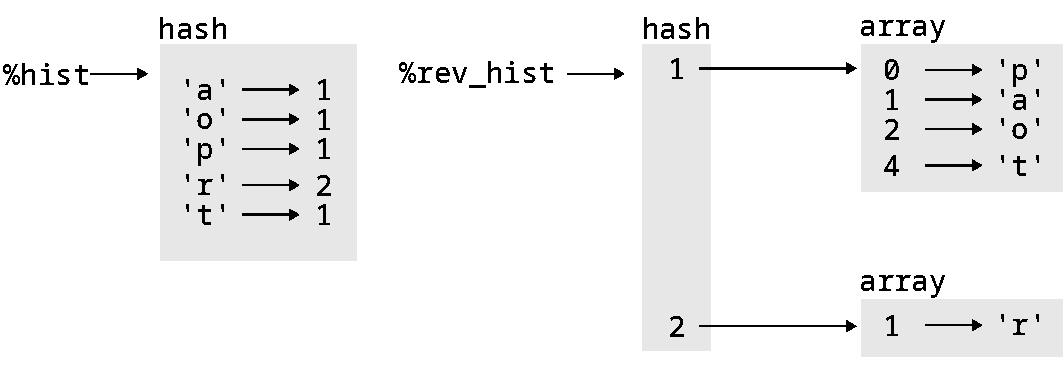
\includegraphics[scale=0.8]{figs/hash1.pdf}}
\caption{Diagrama de estado.}
\label{fig.hash1}
\end{figure}

La figura~\ref{fig.hash1} es un estado de diagrama que muestra a \verb|%hist| 
y a \verb|%rev-hist|. Un hash se representa como una caja con el tipo {\tt hash}
encima y los pares clave-valor dentro.
\index{state diagram}
\index{diagram!state}

Los arrays pueden ser valores en un hash, como este ejemplo muestra, pero
no pueden ser claves. Si intentas hacerlo, probablemente termines con una clave
que contiene solo un elemento del array, pero no lo que esperabas:

\begin{verbatim}
my @a = 'a' .. 'c';
my %h;
%h{@a} = 5;
say %h;  # -> a => 5, b => (Any), c => (Any)
\end{verbatim}

Aquí, Perl interpretó la asignación \verb|%h{@a} = 5;|
como una asignación de rebanada, i.e., asumió que intentamos
poblar tres artículos de una vez, una para cada elemento del
array.

\index{hash!function}
\index{hashable}

Como se mencionó anteriormente, un hash se implementa usando 
una función hash y significa que las llaves tienen
que ser {\tt hashable}\footnote{Esto no es del todo verdad.
Las claves de un hash ``normal``deben ser del tipo hashable
y por lo tanto, inmutable. Hay otro tipo de hash, objetos hash,
para los cuales la necesidad de tener claves inmutables no aplica.}.
Una {\bf función hash} es una función que toma un valor (de cualquier tipo)
y devuelve un número entero. Los hashes usan estos enteros, llamados valores
de hash, para almacenar y buscar pares clave-valor.
\index{immutability}

Este sistema funciona bien si las claves son inmutables. Pero si las claves
son mutables, como con los arrays, cosas extrañas pasarían. Por ejemplo,
cuando creas un par clave-valor, Perl aplicaría una función hash a la clave
y la almacenaría en la ubicación correspondiente. Si modificas el clave y después
aplica la función hash nuevamente, entonces sería almacenada en una ubicación
diferente. En ese caso, podrías tener dos entradas para la misma clave, o 
no podría ser capaz de encontrar una clave. En ambos casos, el hash
no funcionaría correctamente.

Esa es la razón por la cual las claves deben ser hashable, y porqué
los tipos mutables como los arrays no lo son. Así que Perl hará algo más 
que puede ser útil (tal como crear tres artículos de hash distintos en el
ejemplo anterior), pero no aplicará la función hash al array. 
  
Dado que los hashes son mutables, ellos no pueden ser usados como claves,
pero {\em pueden} usarse como valores, así que puedes tener hashes anidados.

\section{Memos}
\label{memoize}
\index{memoize}
\index{cache}
\index{memo}
\index{Fibonacci}

Si jugueteaste con la subrutina {\tt fibonacci} en la 
Sección~\ref{one.more.example}, probablemente notaste que 
mientra más grande el argumento, más tiempo toma la subrutina
para ejecutarse. Además, el tiempo de ejecución aumenta extremadamente
rápido.
\index{Fibonacci!function}
\index{function!Fibonacci}

Para entender el porqué, considera la figura~\ref{fig.fibonacci},
la cual muestra la {\bf gráfica de llamada} para {\tt fibonacci} 
con {\tt n=4}.

\begin{figure}
\centerline
{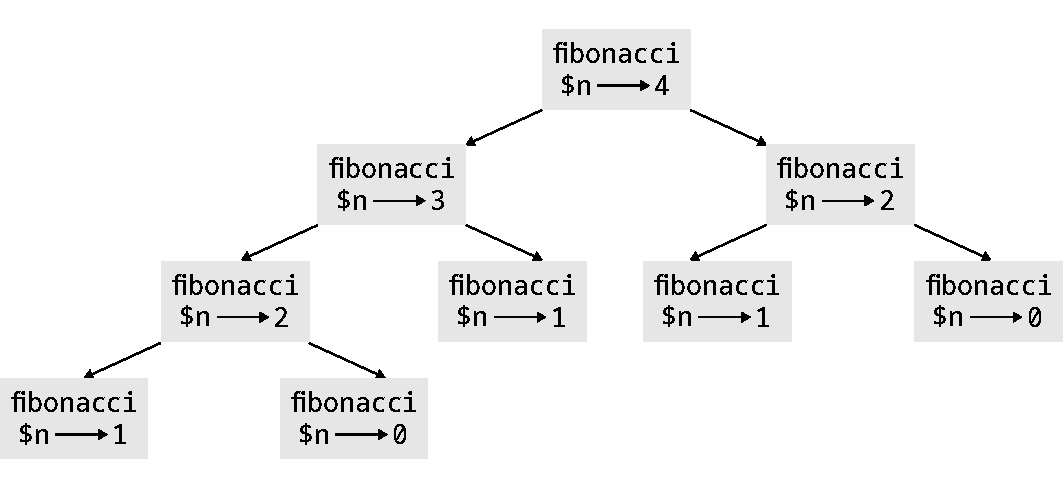
\includegraphics[scale=0.7]{figs/fibonacci.pdf}}
\caption{Gráfica de llamada.}
\label{fig.fibonacci}
\end{figure}

Una gráfica de llamada muestra un conjunto de cuadros de 
una subrutina, con líneas que conectan cada cuadro a los 
cuadros de las funciones que llamas. En la parte superior
de la gráfica, {\tt fibonacci} con \verb|$n=4| llama a \verb|fibonacci|
con \verb|$n=3| y con \verb|$n=2|. En cambio, {\tt fibonacci} con
\verb|$n=3| llama a {\tt fibonacci} con \verb|$n=2| y a \verb|$n=1|,
etcétera.
\index{function frame}
\index{frame}
\index{call graph}

Cuenta cuántas veces {\tt fibonacci(0)} y {\tt fibonacci(1)} 
son llamadas. Esta es una solución ineficiente al problema,
y se vuelve peor a medida que el argumento crece.
\index{memo}

Una solución es mantener un registro de los valores que ya se han
calculado al almacenarlos en un hash. Un valor que se ha computado
y se almacena para uso posterior se conoce como un {\bf memo}. 
Aquí presentamos una versión ``memoizada`` de {\tt fibonacci}:
\index{Fibonacci!memoized}

\begin{verbatim}
my %conocidos = 0 => 1, 1 => 1;
say fibonacci(10);
sub fibonacci ($n) {
    return %conocidos{$n} if %conocidos{$n}:exists;
    %conocidos{$n} = fibonacci($n-1) + fibonacci($n-2);
    return %conocidos{$n};
}
\end{verbatim}
%

\verb|%conocidos| es un hash que mantiene un registro
de los números Fibonacci que ya sabemos. Comienza con dos
artículos: 0 y 1, los cuales mapean a 1.

Cuando se llama a {\tt fibonacci}, la subrutina chequea a
\verb|%known|. Si el resultado ya existe, lo devuelve inmediatamente.
De lo contrario, tiene que computar el nuevo valor, 
agregar al hash, y devolverlo.

Si ejecutas esta versión de {\tt fibonacci} y la comparas con
la original, encontrarás que es mucho más rápida, especialmente
para un argumento grande (por ejemplo, mayor que 30).

\index{cache}
\index{memoize}
La memoización es una forma de \emph{caché}, i.e., almacenar en 
memoria el resultado de una computación (presumiblemente costosa)
para evitar computarla nuevamente. Este proceso es algunas veces 
llamado ``negociación de memoria por ciclos de CPU.`` En algunos 
casos, tal como nuestro ejemplo recursivo de Fibonacci, la ganancia
es absolutamente inmensa: calcular el número Fibonacci 100$^{o}$
tomaría billones de años con la subrutina recursiva original
y toma solo segundos con la versión memoizada. 

Nota que en el caso específico de la función Fibonacci,
estamos almacenando valores para cada entero sucesivo; podría
haber memoizado los números Fibonacci en un array en lugar de 
un hash (y podría ser hasta un poco más eficiente), pero usar
un hash para tal propósito es una solución más general, 
lo cual funciona hasta cuando las claves del memo no son
enteros consecutivos.

Como ejercicio, intentar escribir la subrutina {\tt fibonacci}
usando un array en lugar de un hash para memoizar los números
Fibonacci ya calculados.


\section{Hashes como Tablas de Despacho}
\label{dispatch}

Puede necesitar lanzar alguna acción dependiendo en el valor
de un parámetro recibido por el programa. Para hacer eso,
podrías usar una serie de sentencias
\verb'if {...} elsif {...} else {...}' como esta:

\begin{verbatim}
sub ejecuta-parar   { ... };
sub ejecuta-iniciar { ... };
my $param = obtén-param;
if $param eq "parar" {
    ejecuta-parar;
} elsif $param eq "iniciar" {
    ejecuta-iniciar;
} elsif $param = "a" {
    say $ayuda;
} elsif $param = "ayuda" {
    say $ayuda;
} elsif $param = "v" {
    $verbose = True;
} else {
    die "Opción desconocida $param";
}
\end{verbatim}

Esta estrategia es aburrida y sujeta a errores. El uso de 
una tabla de despacho es usualmente una solución más simple.

Una tabla de despacho es una estructura de datos que mapea 
identificadores a referencias códigos o objetos de subrutinas.
Si se aplica al escenario anterior, podría lucir así:

\begin{verbatim}
sub ejecuta-parar   { ... };
sub ejecuta-iniciar { ... };
my %despacho = (
    parar   => &ejecuta-parar,
    iniciar => &ejecuta-iniciar,
    a       => { say $ayuda; },
    ayuda   => { say $ayuda; },
    v       => { $verbose = True;},
);
my $param = obtén-param();
die "Opción desconocida $param" unless %despacho{$param}:exists;
%despacho{$param}(); # ejecuta la acción especificada en %despacho
\end{verbatim}

El hash \verb|%despacho| define la acción dependiendo en el 
parámetro usado como una clave. La sentencia \verb|%despacho{$param}()|
llama la acción requerida.

Esta estrategia es un poco más concisa y más limpia, pero existen 
otras ventajas. Es más fácil de mantener: si necesitas agregar
una opción, solo necesitas agregar una entrada al hash y evitas
agregar código en el medio de una cadena complicada de sentencias
\verb'if {...} elsif {...} else {...}' lo cual podría estropear algo.

Otra ventaja es que la tabla de despacho puede modificarse
dinámicamente durante el tiempo de ejecución, por ejemplo 
dependiendo en ciertas circunstancias externas (por ejemplo el día
del mes cuando el programa se ejecuta) o de acuerdo a un 
archivo de configuración. Esto significa que es posible 
modificar el comportamiento de un programa dinámicamente 
después del tiempo de compilación, mientras todavía se
ejecuta. Esto abre el camino a algunas técnicas avanzadas de
programación que están fuera del alcance de este libro.

Nota que hemos usado hashes para nuestras tablas de despacho,
y esta es la manera más común de implementarlas. Si hace sentido
tener pequeños enteros como claves, podrías también implementar
una tabla de despacho como un array. Este es el caso, por ejemplo,
los artículos numerados de un menú donde al usuario se le incita
a teclear un número para indicar la opción de menú a activar.


\section{Variables Globales}
\index{global variable}
\index{variable!global}
\index{lexical variable}
\index{variable!lexical}

En el ejemplo anterior sobre Fibonacci memoizado, el hash \verb|%conocidos|
es creado fuera de la subrutina, así que pertenece al 
paquete principal entero. Tales variables con conocidas
como {\bf globales} porque pueden accederse desde cualquier
otra función. A diferencia de variables lexicales ``locales``, 
las cuales desaparecen cuando sus ámbitos terminan, las 
variables globales persisten de una llamada de subrutina 
a la siguiente.
\index{flag}

Es común usar variables globales como {\bf banderas} (\emph{flags} en inglés);
es decir, variables booleanas que indican si una condición es
verdadera. Por ejemplo, algunos programas usan banderas nombradas
\verb|$verbose| para controlar el nivel de detalle en la salida de texto:

\begin{verbatim}
my $verbose = True;
sub ejemplo1 {
    say 'Ejecutando ejemplo1' if $verbose;
    # ...
}
\end{verbatim}
%

Las variables globales son también usadas para variables
de entorno y parámetros que se pasan al programa, como 
para almacenar una estructura de datos que es la pieza central
de un programa, para evitar copiarla cuando se pasa como un 
argumento a las subrutinas.

Pero, a parte de esos casos específicos, es usualmente
considerado mala práctica usar variables globales, porque
crea dependencias y comportamientos de ``acciones a distancia``
inesperados entre varias partes de un programa y puede conducir
a errores que son difícil de encontrar.

En el caso de nuestra subrutina \verb|fibonacci| memoizada,
el hash \verb|%conocidos| es útil solo dentro de la subrutina.
Podemos mejorar la implementación al usar el declarador \verb|state|
dentro de la subrutina:
\index{state}
\index{Fibonacci!memoized with a state variable}

\begin{verbatim}
say fibonacci(10);
sub fibonacci ($n) {
    state %conocidos = 0 => 1, 1 => 1;
    return %conocidos{$n} if %conocidos{$n}:exists;
    %conocidos{$n} = fibonacci($n-1) + fibonacci($n-2);
    return %conocidos{$n};
}
\end{verbatim}
%
El declarador \verb|state| hace la variable local a la subrutina
y persistente de una llamada de la subrutina a la otra: la línea de
código con la sentencia \verb|state| se ejecuta una sola vez 
(en la primera llamada de la subrutina) y el contenido de la 
variable, el hash \verb|%conocidos| en este caso, se mantiene
de una llamada a la siguiente.


\section{Depuración de Programas}
\index{debugging}

A medida que trabajas con conjuntos de datos (\emph{datasets}) más grandes,
puede volverse tedioso e inmanejable depurar con solo la impresión y chequeo
de la salida manualmente. Aquí presentamos algunas sugerencias para depurar
conjuntos de datos grandes:

\begin{description}

\item[Reduce la entrada] Si es posible, reduce el tamaño de
tu conjunto de datos. Por ejemplo, si el programa
lee un archivo de texto, comienza con las primeras 10 líneas, o con
el ejemplo más pequeño que puedas encontrar. Puedes editar los archivos
o (mejor aún) modificar el programa para que lea solo las primeras {\tt n}
líneas.

Si hay un error, puedes reducir {\tt n} al valor más pequeño que manifiesta
el error, y después incrementarlo gradualmente a medida que encuentras
y arreglas los demás errores.

\item[Chequea los resúmenes y tipos] En lugar de imprimir y chequear el conjunto
de datos, considera imprimir resúmenes de los datos: por ejemplo,
el número de artículos en un hash o el total de una lista de 
números.

Una causa común de los errores al tiempo de ejecución es una valor 
que no es del tipo correcto. Para depurar este tipo de error, es 
usualmente suficiente con imprimir el tipo de un valor (piensa sobre
el método {\tt .WHAT}).
\index{WHAT}

Es usualmente útil agregar tipos a tus variables. Donde espera una
cadena de texto, asegúrate de escribir la variable o el parámetro 
de la subrutina con {\tt Str}. Si espera un entero, escríbelo 
con {\tt Int}. Si espera un {\tt Int} de un cierto rango, 
crea un subconjunto para el mismo como en la Sección~\ref{guardian} (p.~\pageref{guardian}) 
y agrega ese tipo a la variable.
\index{subset!type}
\index{type subset}

\item[Escribe autochequeos]  Algunas veces puedes escribir código para
chequear errores automáticamente. Por ejemplo, si estás calculando
el promedio de una lista de números, podrías chequear que el 
resultado no sea mayor que el elemento más grande en la lista o menor
que el elemento mas pequeño. Esto se conoce como ``comprobación de
validez`` porque detecta aquellos resultados que son ``inválidos``.
\index{sanity check}
\index{consistency check}

Otro tipo de chequeo compara los resultados de dos computaciones
diferentes para ver si son consistentes. Esto se llama
``comprobación de consistencia``.

\item[Formatea la salida] Formatear la salida de un proceso de
depuración puede facilitar la detección de errores. Vimos un ejemplo
en la Sección~\ref{factdebug}. La función {\tt dd} muestra detalles
útiles de una estructura de datos compuesta o compleja.

\index{dd function}
\index{function!dd}

\end{description}

Nuevamente lo repito: el tiempo que inviertes en andamiaje puede 
reducir el tiempo que pierdes en depuración.
\index{scaffolding}


\section{Glosario}

\begin{description}

\item[Mapeo] Una relación en la cual cada elemento de un
conjunto corresponde a un elemento de otro.
\index{mapping}

\item[Hash] Un mapeo de las claves a sus valores correspondientes.
\index{hash}

\item[Par clave-valor] La representación de un mapeo de una sola clave
a su valor.
\index{key-value pair}

\item[Artículos] En un hash, otro nombre para un par clave-valor.
\index{item!hash}

\item[Clave] Un objeto que aparece en un hash como la primera parte
de un par clave-valor.
\index{key}

\item[Valor] Un objeto en un hash que aparece como la segunda parte de 
un par clave-valor. Esto es más específico que nuestro uso previo de
la palabra ``valor``.
\index{value}

\item[Implementación] Una forma de realizar una computación.
\index{implementation}

\item[Tabla hash] El algoritmo usado para implementa hashes.
\index{hashtable}

\item[Función hash] Una función usada por una tabla hash para computar
la ubicación de una clave.
\index{hash!function}

\item[Hashable] Un tipo que contiene una función hash. Los tipos inmutables
como los números y las cadenas de texto son hashables; los tipos
mutables como los array y los hashes no lo son.
\index{hashable}

\item[Búsqueda] Una operación de un hash que toma una clave y encuentra
el valor correspondiente.
\index{lookup}

\item[Búsqueda inversa] Una operación de un hash que toma un valor 
y encuentra una o más claves que mapean al valor.
\index{reverse lookup}

\item[Gráfica de llamada] Una diagrama que muestra cada marco creado 
durante la ejecución de un programa, con una flecha de cada función
que hace la llamada a la función que se llama.
\index{call graph}
\index{diagram!call graph}

\item[Memo] Un valor que se calcula para evitar computaciones futuras
innecesarias.
\index{memo}

\item[Memoizar] Almacenar un valor calculado en la memoria para
evitar cálculos posteriores del mismo. La memoización es una forma
de caché.
\index{memoize}

\item[Variable global]  Una variable definida fuera de cualquier subrutina
u otro bloque. Las variables globales pueden accederse desde cualquier
subrutina.
\index{global variable}

\item[Bandera] Una variable Booleana que se usa para indicar si una 
condición es verdadera.
\index{flag}

\end{description}


\section{Ejercicios}

\begin{exercise}
\label{wordlist2}
\index{set!membership}
\index{membership!set}

Escribe una subrutina que lea las palabras en \emph{words.txt}
y las almacene como claves de un hash. (No importa cuales sean los
valores.) Después puedes usar el adverbio {\tt exists} como una manera
rápida de chequear si una cadena de texto se encuentra en el hash.

Si hiciste el Ejercicio~\ref{bisection}, puedes computar la
rapidez de esta implementación con un hash y la búsqueda binaria.

Solución: \ref{sol_wordlist2}

\end{exercise}


\begin{exercise}
\label{mem_ackerman}
Memoiza la función Ackermann del Ejercicio~\ref{ackermann}
y observa si la memoización hace posible evaluar la subrutina
con argumentos más grandes. Pista: no.
Solución: \ref{sol_mem_ackerman}.
\index{Ackermann function}
\index{function!ack}

\end{exercise}



\begin{exercise}
\index{duplicate}
\label{has_duplicates_hash}

Si hiciste el Ejercicio~\ref{has_duplicates}, ya tienes una función
llamada \verb|tiene-duplicados| que toma una lista como un 
parámetro y devuelve {\tt True} si cualquier objeto aparece más
de una vez en la lista.

Usa un hash para escribir un versión más rápida y simple
de \verb|tiene-duplicados|.
Solución: \ref{sol_has_duplicates_hash}.

\end{exercise}


\begin{exercise}
\label{exrotatepairs}
\index{letter rotation}
\index{rotation, letters}

Dos palabras son ``pares rotativos`` si puedes rotar una de ellas
y conseguir la otra (ver \verb"rotar-palabra" en 
Ejercicio~\ref{rotate}) usando el cifrado César.
\index{Caesar cipher}

Escribe un programa que una lista de palabras (por ejemplo, {\tt words.txt}
y encuentre todos los pares rotativos.
Solución: \ref{sol_exrotatepairs}.

\end{exercise}


\begin{exercise}
\label{homophones}
\index{Car Talk}
\index{Puzzler}

Este es otro Puzzler de {\em Car Talk} 
(\url{http://www.cartalk.com/content/puzzlers}):

\begin{quote}

Esto fue enviado por una persona llamada Dan O'Leary. Recientemente,
él encontró una palabra monosilábica de cinco letras que tiene la 
siguiente propiedad única. Cuando se remueve la primera letra, las 
letras restantes forman un homófona de la palabra original, es decir,
una palabra que suena exactamente igual. Reemplaza la primera letra,
es decir, colócala devuelta y remueve la segunda letra y el resultado
es aún otra homófona de la palabra original. Y la pregunta es, cuál es
la palabra?

Ahora te daré un ejemplo que no funciona. Miremos a la palabra de cinco
letras, `wrack`. W-R-A-C-K, como en `wrack with pain'. Si remuevo la primera
letra, me quedo con una palabra de cuatro letras, 'R-A-C-K'. Como en, 
`Holy cow, did you see the rack on that buck!It must have been a nine-pointer!' 
Es un homófono perfecto. Si pones la `w` devuelta, y remueve la `r`, te quedas
con la palabra `wack`, la cual es una palabra real, es solamente no una homófona de
las otras dos palabras.

Pero existe, sin embargo, por lo menos una palabra que Dan y todos
nosotros conocemos, que producirá dos homófonas si remueve una de las primeras
dos letras para crear dos nuevas palabras de cuatro letras. La pregunta es,
cuál es la palabra?
\end{quote}
\index{homophone}
\index{reducible word}
\index{word, reducible}

Puedes usar el hash del Ejercicio~\ref{wordlist2} más arriba para
chequear si una cadena de texto se encuentra {\tt words.txt}.

Para chequear si dos palabras son homófonas, puedes usar el 
Diccionario de Pronunciación CMU. Puedes descargarlo de 
\url{http://www.speech.cs.cmu.edu/cgi-bin/cmudict}.
\index{CMU Pronouncing Dictionary}

Escribe un programa que enumere todas las palabras en {\tt words.txt}
(o en el diccionario CMU) que resuelva el Puzzler.
Solución: \ref{sol_homophones}.

\end{exercise}





\chapter{Caso Práctico: Selección de Estructura de Datos}
\label{data_struct_sel}

A esta altura ya aprendiste sobre las estructuras de datos principales
de Perl, y has visto algunos de los algoritmos que las usan.

Este capítulo presenta un caso práctico con ejercicios que te dejan 
pensar acerca de la elección de estructuras de datos y practicar 
usándolas.

Pero primero, me gustaría discutir brevemente dos estructuras condicionales
que hemos ignorado hasta ahora y proveer nuevas posibilidades sobre las
signaturas de una subrutina.
\index{signature}

\section{El Operador Condicional Ternario}
\label{ternary operator}
\index{ternary conditional operator}

Considera el siguiente código que verifica el valor de un
número entero positivo:

\begin{verbatim}
my $result;
if $num < 10 {
    $result = "Un dígito";
} else {
    $result = "Más de un dígito";
}
say $result;
\end{verbatim}

Esto es bien simple, pero un poco largo. Esto puede escribirse
en una sola línea de código en la siguiente forma:

\begin{verbatim}
say $num < 10 ?? "Un dígito" !! "Más de un dígito";
\end{verbatim}

El operador está conformado por dos partes: {\tt ??} y {\tt !!},
los cuales separan tres expresiones (de ahí su nombre de ``operador ternario``):
\index{ternary operator}
\index{operator!ternary}
\begin{itemize}
\item La condición a ser evaluada (?`es \verb|$num| menor que 10?);
\item La expresión que define el valor si la condición es verdadera;
\item La expresión que define el valor si la condición es falsa.
\end{itemize}

Esta sentencia chequea si \verb|$num| es menor que 10 y, si esto es verdadero,
imprime ``Un dígito``; si la condición es falsa, entonces imprime ``Más de un dígito``.

Este operador no provee una funcionalidad nueva; solo ofrece una sintaxis
más concisa.

Es posible anidar varios operadores ternarios para examinar múltiples opciones
sucesivamente:
\index{ternary conditional operator, nesting}

\begin{verbatim}
say $valor < 10    ?? "Un dígito"     !! 
    $valor < 100   ?? "Dos dígitos"   !!
    $valor < 1000  ?? "Tres dígitos"  !!
                      "Más de tres dígitos";
\end{verbatim}

Esta construcción es una forma de sentencia conocida algunas
veces como una \emph{sentencia de switch} porque el lenguaje
C y muchos lenguajes derivados del mismo usan la palabra clave
{\tt switch} para describir una condicional con opciones múltiples.
\index{switch statement}

Esto es mucho más conciso y usualmente más conveniente que las condicionales
anidadas {\tt if ... después ... else}, pero la siguiente sección provee un
tipo de sentencia {\tt switch} mucho más poderosa.

\section{La Sentencia ``Switch'' {\tt given ... when}}
\label{given_when}
\index{given statement}
\index{when statement}
\index{switch statement}

Perl~6 tiene una sentencia ``switch'', escrita con las palabras claves 
{\tt given} y {\tt when}. La palabra clave {\tt given} introduce la variable
o expresión que será puesta a prueba, y cada una de las sentencia {\tt when}
especifica una condición seguida por un bloque que se ejecutará si la 
condición es verdadera. Por defecto, el proceso para cuando la primera
con la primera condición que es satisfecha.

El ejemplo más arriba podría escribirse como sigue:

\begin{verbatim}
given $value {
    when 0..9      { say "Un dígito" }
    when $_ < 99   { say "Dos dígitos" }
    when /^\d**3$/ { say "Tres dígitos" }
    default        { say "Más de tres dígitos" }
}
\end{verbatim}

La sentencia \verb|given $valor| ``topicaliza`` el argumento, i.e., 
asigna el contexto de \verb|$valor| a la variable tópico \verb|$_|
(o, más precisamente, crea un sobrenombre del mismo a través de 
la variable \verb|$_|). El argumento de {\tt given} es una variable simple
en el ejemplo más arriba, pero puede ser una expresión compleja cuya evaluación
se almacena en \verb|$_|. Cada una de las condiciones {\tt when} es
chequeada contra \verb|$_|. He escrito estas condiciones en tres formas
sintácticas diferentes para ilustrar algunas de las varias posibilidades:
\index{topical variable}
\index{alias}
\begin{itemize}
\item La primera chequea contra \verb|$_| (implícitamente) contra el
rango \verb|0..9|.
\index{range operator}
\item La segunda compara explícitamente \verb|$_| con 99.
\item La tercera usa un regex para chequear si \verb|$_| tiene
tres dígitos.
\index{regex}
\item La sentencia \verb|default| se ejecuta solo si las otras condiciones
han fallado.
\index{default statement}
\end{itemize}

Solo un mensaje será imprimido, porque el proceso de coincidencia para tan
pronto una de las condiciones ha sido satisfecha, y la cláusula \verb|default|
se ejecutará solo si las otras condiciones fallaron.

Si no hay un operador específico en la cláusula {\tt when}, entonces realizará
una coincidencia inteligente de la expresión en la la cláusula {\tt when} contra
 \verb|$_|:
\index{smart match}

\begin{verbatim}
when $foo { ... }
# equivalente a: when $foo ~~ $_ { ... }
\end{verbatim}

Nota que la palabra clave {\tt given} no hace más que topicalizar
su argumento para el resto del bloque. Las cláusulas {\tt when} son las
que hacen el trabajo pesado. De hecho, podrías usar las cláusulas {\tt when}
sin {\tt given} provisto que asignes el valor correcto a \verb|$_|, lo cual,
como podrás recordar, puede hacerse con un bloque {\tt for}:
\index{for block}

\begin{verbatim}
my $val = 7;
for $val { 
    when 0..6 { say "menos que"}
    when 7 {say "Exacto";} 
    when 8..* {say "mayor que";}
}
\end{verbatim}

\index{proceed clause}
Es posible añadir una cláusula {\tt proceed} al final de cualquier de los
bloques de código condicionales para prevenir que el proceso pare
después que el bloque de código haya sido exitoso. Por ejemplo, podrías 
escribir esto:

\begin{verbatim}
given $valor {
    when 0..9      { say "Un dígito" }
    when 10..99    { say "Dos dígitos"; proceed }
    when 42        { say "La respuesta del sentido de la vida y a todo el universo" }
    when /^\d**3$/ { say "Tres dígitos" }
    default        { say "Más de tres dígitos" }
}
\end{verbatim}

En este ejemplo, si \verb|$valor| es 42, dos mensajes se imprimirán,
"Dos dígitos" y "La respuesta del sentido de la vida y a todo el universo"
porque la cláusula {\tt proceed} en el segundo bloque de código 
evita que el proceso termine con la primera coincidencia exitosa.

Grandioso, pero hay un problema. La cláusula {\tt proceed} debería usarse
con cuidado, dado que puede fácilmente conducir a resultados inesperados.
De hecho, \emph{el código de más arriba es incorrecto}: si \verb|$valor| tiene
dos dígitos pero no es 42 (si es, digamos, 43), el bloque {\tt default} 
también se ejecutará, porque la única coincidencia exitosa tenía la cláusula
{\tt proceed}, y dirá que hay más `Más de tres dígitos'' aunque esto es
obviamente falso.

\label{proceed_ex}
Como un ejercicio, prueba el código anterior con varios valores y
intenta encontrar una manera de arreglar el error con la cláusula {\tt proceed}.

Solución: \ref{sol_proceed_ex}

\section{Subrutinas con Parámetros Nombrados y Opcionales}

% Revise this definition to make it clearer.
Las subrutinas que hemos visto hasta ahora han usado parámetros
\emph{de posición}, i.e., parámetros en los cuales la atadura (\emph{binding} en inglés) 
con los argumentos de la subrutina depende en el orden de los mismos
dentro de la lista de argumentos y en la signatura de la función. 
Usualmente esto es perfectamente normal cuando el número de argumentos
pasado a la subrutina es pequeño (digamos, tres o menos).
\index{positional parameter}
\index{parameter!positional}
\index{signature}

Cuando la signatura de la subrutina se vuelve larga, el uso de 
argumentos de posición podría volverse complicado y propenso a
errores.

\subsection{Parámetros Nombrados}
\index{named parameter}
\index{parameter!named}

Los argumentos nombrados pueden suministrarse en cualquier orden:
el nombre del parámetro está atado al argumento del mismo nombre.
Por ejemplo:

\begin{verbatim}
sub dividir (:$dividendo, :$divisor where $divisor != 0) {
     return $dividendo/$divisor;
}
say dividir(dividendo => 2048, divisor => 128);      # -> 16
# o:
say dividir(divisor => 128, dividendo => 2048);      # -> 16
\end{verbatim}

Los argumentos son suministrados en la llamada de la subrutina como una
lista de pares usando la sintaxis de constructor de pares. En la signatura,
los parámetros son extraídos en la signatura con la sintaxis de "colon-pair":
el parámetro \verb|$dividendo| está atado al valor del par cuya clave es 
``dividendo`` (2048), y \verb|$divisor| está similarmente atado a 128, 
sin importar el orden de los argumentos en la llamada de la subrutina.
\index{colon-pair syntax}
\index{pair constructor}

Estos parámetros nombrados son especialmente útiles cuando el número de
argumentos es grande. Por ejemplo, no hemos hablado de la programación
orientada a objetos todavía (ver Capítulo~\ref{objects}), pero esto es como
podríamos crear un objeto de la clase (definida por el usuario) Rectángulo:

\begin{verbatim}
my $rect = Rectángulo.new( 
    origen_x  => 100, 
    origen_y  => 200, 
    ancho     => 23,
    longitud  => 42,
    color     => 'negro'
);
\end{verbatim}

Claramente, el uso de cinco parámetros de posición no sería práctico.

\subsection{Parámetros Opcionales}
\index{optional parameter}
\index{parameter!optional}
\index{variadic subroutine}
\index{signature}

Algunas veces, el número actual de argumentos no se conoce
con antelación: por ejemplo, una subrutina puede llamarse con 
un número variable de argumentos. Tal subrutina se conoce como
\emph{variádica}. Puedes definir un parámetro para que sea opcional
al colocar un signo de interrogación en frente del mismo en la
signatura de la subrutina:

\begin{verbatim}
sub my-sub($x, $y?) {  # simple parámetro opcional
    if $y.defined {
        say "El segundo parámetro ha sido suministrado y definido";
    } else {
        say "El segundo parámetro no ha sido suministrado";
    }
    # ...
}
\end{verbatim}

\index{positional parameter}
\index{parameter!positional}
Al usar parámetros de posición, los parámetros opcionales siempre
tienen que ser los últimos en la lista (después de aquellos que 
son argumentos).

Un parámetro puede también hacerse opcional al suministra un:
{\bf valor por defecto}:
\index{default value}
\index{default parameter}
\index{parameter!default value}

\begin{verbatim}
sub mi-log($número, $base = e) {    # e es una constante predefinida
                                    # $base es un parámetro opcional
    return log($número) / log($base);
}
say mi-log(4);       # Logaritmo natural (base e)  -> 1.38629436111989
say mi-log(32, 2);   # Logaritmo en base 2         -> 5
say mi-log(100, 10); # Logaritmo común (base 10)   -> 2
\end{verbatim}

Aquí, si el segundo argumento no se suministra, el valor por defecto 
(\emph{e}) es usado. Inversamente, si hay un segundo argumento, este
{\bf anula} el valor por defecto.

\index{slurpy parameters}
\index{parameter!slurpy}
\label{slurpy_parameters}
En algunas ocasiones, tener parámetros opcionales o por defecto no
es suficiente. Por ejemplo, la subrutina puede tener que procesar una 
lista que contiene un número indeterminado de valores. Para situaciones
como esta, puedes usar un \emph{parámetro slurpy}, i.e., un tipo de
array colocado al final de la lista de parámetros que consumirá todos los 
argumentos restantes. Este tipo de parámetro slurpy usa el sigilo \verb|*@|.
En el ejemplo siguiente, la subrutina toma un parámetro mandatario
(el primer número de la lista) y un lista de argumentos adicionales
que serán almacenados en el array \verb|@resto|:
\index{twigil}

\begin{verbatim}
sub mi-suma($primer-num, *@resto) {
    say @resto;                      # -> [3 4 5 12 17]
    return $primer-num + [+] @resto;
}
say mi-suma 1, 3, 4, 5, 12, 17;      # -> 42 
\end{verbatim}

Otros ejemplos de los parámetros slurpy se han proveído
en la Sección~\ref{sol_exercise_queue}.

\section{Análisis de la Frecuencia de Palabras}
\label{analysis}

Ahora, hablemos del caso práctico.

Como es habitual, deberías por lo menos intentar los
ejercicios antes de leer las soluciones sugeridas, las cuales
se proveen en las secciones siguientes de este capítulo.

\begin{exercise}

Escribe un programa que lee un archivo, descompone cada línea en palabras,
remueve los espacios en blanco y signos de puntuación de la palabra,
y las convierte a palabras minúsculas.

\end{exercise}


\begin{exercise}
\index{Project Gutenberg}

Dirígete a Project Gutenberg (\url{http://gutenberg.org}) y descarga tu 
copia de libro favorito en formato de texto simple.
\index{plain text}
\index{text!plain}

Modifica tu programa del ejercicio previo para que lea el libro que descargaste,
salta sobre la información de la cabecera al principio del archivo, y procesa el 
resto de las palabras como lo hiciste anteriormente.

Después modifica el programa para que cuente el número total de palabras en
el libro, y el número de veces que cada palabra es usada.
\index{word frequency}
\index{frequency!word}

Imprime el número de palabras diferentes usadas en el libro. Compara
libros diferentes por autores diferentes, escritos en eras diferentes. 
?`Cuáles autores usan el vocabulario más extenso?
\end{exercise}


\begin{exercise}

Modifica el programa del ejercicio anterior para que imprima las
20 palabras más frecuentemente usadas en un libro dado,

\end{exercise}


\begin{exercise}

Modifica el programa anterior para que lea una lista de palabras (ver Sección~\ref{wordlist})
y después imprima todas las palabras en el libro que no están en la 
lista de palabras. ?`Cuántas de ellas son errores tipográficos? ?`Cuántas de ellas
son palabras comunes que {\emph deberían} estar en la lista de palabras, y cuántas de
ellas son realmente recónditas?

\end{exercise}


\section{Números Aleatorios}
\index{random number}
\index{number, random}
\index{deterministic}
\index{pseudorandom}

Dada la misma entrada, la mayoría de programas de computadoras generan
la misma salida cada vez y, por lo tanto, se dice que son {\bf deterministas}.
El determinismo es usualmente algo bueno, dado que esperamos que 
la misma computación produzca el mismo resultado. Aunque, para algunas aplicaciones,
queremos que la computadora sea impredecible. Los juegos de computadora
son un ejemplo obvio, pero existen más.

Hacer un programa verdaderamente no determinista resulta ser algo difícil,
pero hay algunas manera de hacerlo parecer por lo menos no determinista. 
Una de ellas es usar algoritmos que generan números {\bf pseudoaleatorios}.
Los números pseudoaleatorios no son verdaderamente aleatorios porque son
generados a través de una computación determinista, pero solo con mirarlos
es imposible distinguirlos de los números aleatorios.

Perl provee funciones tales como {\tt rand} que generan números pseudoaleatorios
(los cuales llamaremos simplemente números ``aleatorios`` de aquí en adelante).
\index{rand function}
\index{function!rand}

La función {\tt rand} devuelve un número aleatorio (del tipo {\tt Num}) entre
0.0 y 1.0 (incluyendo a 0.0 pero no a 1.0). Cada vez que llamas a {\tt rand},
obtienes el número siguiente en una serie larga. Para ver una muestra, ejecuta
este bucle en el REPL:

\begin{verbatim}
say rand for 1..5;
\end{verbatim}

Cuando se usa como un método, {\tt rand} devuelve un número aleatorio entre
0.0 y el valor del invocante. Por ejemplo, {\tt 10.rand} devuelve un número
aleatorio entre 0 y 10 (excluyendo al 10). Podrías intentarlo como un programa
de una sola línea:
\index{one-liner mode}

\begin{verbatim}
$ perl6 -e 'say 10.rand for 1..5'
8.23987158729588
9.83276889381497
2.52313276833335
3.44713459548771
1.82329894347025
\end{verbatim}

Con suerte, deberías obtener una salida diferente a la que obtuve.
Si quieres ejecutar un programa de una sola línea en Windows,
recuerda que necesitarás reemplazar las comillas simples con comillas
dobles.

Para obtener números enteros aleatorios entre 1 y 10, podrías usar 
los métodos {\tt Int} y {\tt rand}:
\index{Int function or method}

\begin{verbatim}
$ perl6 -e 'say 10.rand.Int + 1 for 1..5'
5
10
1
6
3
\end{verbatim}

La función o método {\tt pick} toma un número \verb|$n| y una lista 
como argumentos y devuelve \verb|$n| artículos escogidos aleatoriamente
y sin repetición. Por ejemplo:
\index{pick function or method}

\begin{verbatim}
> say <1 3 4 5 7 9 10 12 14 42>.pick(5);
(5 42 3 4 7)
> say pick 5, <1 3 4 5 7 9 10 12 14 42>;
(42 12 5 1 9)
\end{verbatim}

Si \verb|$n| es mayor o igual al número de artículos de la lista,
entonces todos los elementos de la lista será devueltos en una
secuencia aleatoria.

Para obtener enteros aleatorios únicos en un rango, podrías usar
{\tt pick} en un rango:

\begin{verbatim}
> say pick 5, 1..20;
(5 3 6 18 7)
> say (1..20).pick(5);
(20 4 18 2 7)
\end{verbatim}

Si no especifica la cantidad de números aleatorios, obtendrás un
solo número aleatorio:

\begin{verbatim}
> say (1..20).pick;
19
\end{verbatim}
%


\begin{exercise}
\index{histogram!random choice}

Escribe una función nombrada \verb"escoge_del_hist" que toma un
histograma como definido en la Sección~\ref{histogram} y devuelve 
un valor aleatorio del histograma, elegido con una probabilidad 
proporcional a la frecuencia. Por ejemplo, para tres artículos:
\verb|('a', 'a', 'b')|, tu función debería devolver \verb|a| con una
probabilidad de $2/3$ y \verb|'b'| con una probabilidad de $1/3$.
\end{exercise}


\section{Histograma de Palabras}

Deberías intentar solucionar el ejercicio anterior antes
de proceder.

Para el propósito de presentar las soluciones a los ejercicios anteriores,
he usado el texto sencillo de {\em Don Quijote} (1605 y 1615), una novela escrita
por Miguel de Servantes, descargada desde el proyecto Gutenberg
(\url{https://www.gutenberg.org/files/2000/2000-8.txt}) y guardada en
un archivo llamado \emph{quijote.txt}
\footnote{Si tienes algún problema
con el archivo, puede deberse a cambios hecho al formato del mismo por
el proyecto Gutenberg. Para evitar tal problema asociado con cualquier
cambio (y otros cambios futuros), puedes descarga el archivo original
desde este repositorio de Gitlab: \url{https://gitlab.com/uzluisf/piensaperl6/tree/master/suplementos/quijote.txt}}.
Usa el mismo texto si quieres comparar tus soluciones y los resultados con los míos.

% https://github.com/LaurentRosenfeld/thinkperl6/blob/master/Supplementary/emma.txt
\index{de Servantes, Miguel}
\index{Don Quijote}
\index{Project Gutenberg}

\begin{description}
\item {\bf Nota del traductor}:	En {\em Think Perl 6}, el autor usa el texto de la novela
\emph{Emma}, escrita por Jane Austen\footnote{Puedes encontrar el archivo en este repositorio: 
\url{https://github.com/LaurentRosenfeld/thinkperl6/blob/master/Supplementary/emma.txt}.
De igual manera, puedes consultar Think Perl 6 para comparar tus resultados con los del 
autor si decides usar este texto.}. He decidido usar un libro en español porque creo que es más ameno y porque quería saber cuantas palabras tenía el libro \emph{Don Quijote de la Mancha}.
\end{description}

Aquí esta el programa que lee el archivo \emph{quijote.txt} y construye un
histograma de las palabras  en el archivo que pertenecen al libro:
\index{histogram!word frequencies}

\begin{verbatim}
my %histograma;
my $saltar = True; # bandera para saltar la cabecera y 
                   # marcar el final del libro

sub procesar-línea(Str $línea is copy) {
	if defined index $línea, "*** START OF THIS PROJECT" {
		$saltar = False ;
		return;
	}

	return if $línea ~~ / Abela || anonymous /; 
	return if $saltar;
	$línea ~~ s:g/<['-]>/ /;             # Reemplazar guiones y apóstrofos con espacios
	$línea ~~ s:g/<[;:,¡!¿?«».()"_`]>//; # Remover signos de puntuación
	$línea = $línea.lc;                  # Convertir cadena a minúscula
	for $línea.words -> $palabra {
		%histograma{$palabra}++;
	}

	$saltar = True if $línea ~~ /^fin$/; # Marcar el final del libro
}
procesar-línea $_ for "quijote.txt".IO.lines; 
\end{verbatim}

\index{case!lower}
%

El programa lee cada línea del archivo \emph{quijote.txt} file y,
por cada línea, llama a la subrutina \verb|procesar-línea|.

\index{accumulator!histogram}
La subrutina \verb|procesar-línea| salta las líneas de la cabecera
(i.e., todas las líneas hasta que se encuentra la línea que contenga
la cadena de texto ``*** START OF THIS PROJECT``). De igual manera,
también salta cualquier línea que contenga las palabras ``Abela`` o
``anonymous``. La función reemplaza 
los guiones y los apóstrofos con espacios en blanco, remueve varios 
caracteres de puntuación, y convierte la línea a minúscula. Después,
divide la línea en palabras individuales que son almacenadas y 
contadas con un acumulador en el hash \verb|%histograma|.  Al final
asigna verdadero a \verb|$saltar| si la línea contiene solo la 
palabra ``fin``, la cual marca el final del texto.

Para saber si el programa está haciendo lo que esperamos que haga,
podemos mostrar unas entradas del hash \verb|%histograma|:

\begin{verbatim}
# mostrando 20 líneas del histograma
my $cuenta;
for %histograma -> $par {
say sprintf "%-24s %d", $par.key, $par.value;
$cuenta++;
last if $cuenta > 20;

}
\end{verbatim}

Esto imprime lo siguiente:

\begin{verbatim}
ahorcase                 1
descontente              1
regüeldos                1
libras                   5
manteca                  1
suerte                   141
voy                      51
desnudaba                1
xxviii                   2
benevolencia             2
vieren                   3
rebenque                 1
asentado                 2
profetizadas             2
mirábalas                1
lata                     4
cesaría                  1
preguntalle              1
bailado                  2
elogio                   2
codicio                  1
\end{verbatim}

Para contar el número total de palabras (pertenecientes al libro) en el archivo,
podemos añadir los valores en el histograma:

\begin{verbatim}
my $total_palabras = [+] %histograma.values;
say "Hay $total_palabras palabras en el libro.";
\end{verbatim}
%
El número de palabras diferentes es solo el número de artículos en
el hash:

\begin{verbatim}
my $palabras-distintas = %histograma.elems;
say "Hay $palabras-distintas palabras distintas en el libro.";
\end{verbatim}
%
Nota que podrías reducir lo anterior a una línea de código al
interpolar un bloque de código dentro de la cadena de texto de salida:
\index{interpolating a code block in a string}

\begin{verbatim}
say "Hay {%histograma.elems} palabras distintas en el libro.";
\end{verbatim}
%
Y los resultados:

\begin{verbatim}
Hay 381215 palabras en el libro.
Hay 22950 palabras distintas en el libro.
\end{verbatim}
%


\section{Palabras Más Comunes}
\label{most_common_words}

Para encontrar las palabras más comunes en \verb|quijote.txt|,
podemos ordenar el hash \verb|%histograma| de acuerdo a los 
valores (frecuencia de palabras) y extraer las 10 palabras más
frecuentes en un array.
\index{sort}

\begin{verbatim}
my @más_comunes = (sort { %histograma{$^b} cmp %histograma{$^a} }, 
                    %histograma.keys)[0..9];
say $_ for map { "$_ \t%histograma{$_} "}, @más_comunes;
\end{verbatim}

Las funciones {\tt sort} recibe las claves del histograma y su función 
de comparación compara los valores asociados con esas claves. Dado que
usamos la clave \verb|$^b| antes que la clave \verb|$^a|, {\tt sort}
producirá un ordenamiento en orden reverso (descendente). El procedimiento
{\tt sort} completo está colocado dentro de paréntesis, para que el rango 
de subíndices {\tt [0..9]} actúe como una rebanada sobre la lista producida por
{\tt sort} y retiene solo las primeras 10 palabras más frecuentes. El resultado
se almacena en el array \verb|@más_comunes|. La siguiente línea de código 
solo procesa el array para mostrar las palabras y sus frecuencias respectivas.
\index{slice}

Esto muestra la siguiente salida:

\begin{verbatim}
que     20626 
de      18214 
y       18188 
la      10363 
a       9823 
en      8241 
el      8210 
no      6335 
los     4748 
se      4690 
\end{verbatim}
%
Si quieres ver más palabras interesantes, podrías, como un ejercicio
adicional, filtrar el histograma y retener solo las palabras
que tienen más de, digamos, cuatros letras.

El array temporario \verb|@más_comunes| no es realmente necesario.
Podríamos hacer todo el proceso con una sola sentencia:

\begin{verbatim}
say $_ for map { "$_ \t%histograma{$_} "},  
           (sort { %histograma{$^b} cmp %histograma{$^a} }, 
           %histograma.keys)[0..9];
\end{verbatim}

Este es un ejemplo de la programación de tuberías. Este tipo de sentencia
necesita leerse de abajo hacia arriba y de derecha a izquierda. El 
primer paso es \verb|%histograma.keys|, el cual produce una lista de
las claves del histograma; esta lista se suministra a la sentencia {\tt sort}
para producir una lista de las llaves ordenadas (en orden descendente)
de acuerdo a sus valores; una vez que esta parte entre los paréntesis
se ha completado, el rango de subíndices \verb|[0..9]| retiene las 10 
palabras más frecuentes y las administra a la sentencia map, la cual 
produce la lista de palabras y las frecuencias para la salida final.

Déjame agregar una palabra de advertencia: ordenar el histograma
por los valores y escoger los 10 más frecuentes para obtener las
palabras más frecuentes es probablemente la manera más fácil de 
resolver el problema y el código más corto para hacerlo.
Esta es la razón por la cual he usado esta solución aquí. Pero no es la
solución más eficiente desde el punto de vista del tiempo de ejecución,
porque involucra el costo de ordenar un conjunto de datos relativamente
grade, donde solo usamos una parte pequeña de los datos ordenados. Hay
algoritmos mejores para hacer eso desde el punto de vista de la
eficiencia de ejecución, pero son más complicados. Por lo tanto, hay 
un sacrificio entre la eficiencia de código y el rendimiento. Asumiendo que 
esto es código que queremos ejecutar solamente una vez, he favorecido
la eficiencia de código.
\index{data pipeline programming}


\section{Parámetros Opcionales}
\index{optional parameter}
\index{parameter!optional}

Vimos anteriormente en este capítulo que las subrutinas pueden tomar
parámetros opcionales. Podemos usar esta funcionalidad para escribir
una subrutina que imprime las palabras más comunes en el 
hash \verb|%histograma| extraído desde \emph{quijote.txt}.

\begin{verbatim}
mostrar-más-comunes(%histograma, 5);

sub mostrar-más-comunes( %hist, Int $num = 10 ) {
    say $_ for map { "$_ \t%hist{$_} "}, 
    (sort { %hist{$^b} cmp %hist{$^a} },
    %hist.keys)[0..$num - 1];
}
\end{verbatim}

Esto mostrará las 5 palabras más comunes de la lista más
arriba (Sección~\ref{most_common_words}). Si la llamamos
sin el segundo parámetro:

\begin{verbatim}
mostrar-más-comunes(%histograma);
\end{verbatim}

obtendremos las 10 palabras más comunes (misma lista como la
que mostramos en la Sección~\ref{most_common_words}), porque el 
valor por defecto para el segundo parámetro es 10.

\section{Diferencia de Hashes}
\label{hashsub}
\index{hash!subtraction}
\index{subtraction!hash}

Encontrar las palabras en \emph{quijote.txt} que no están en la lista
de palabras {\tt lemario.txt} es un problema que podrías reconocer como una 
diferencia de conjuntos; es decir, queremos encontrar todas las palabras
en un conjunto (las palabras en \emph{quijote.txt}) que no están en el
otro (las palabras en \emph{lemario.txt}).

La subrutina {\tt sustraer} toma los hashes \verb|%princ| y \verb|%dicc|
y devuelve un nuevo hash que contiene todos las claves de \verb|%princ|
que no están en \verb|%dicc|. Dado que no nos importan los valores, asignamos
1 a todas la claves.

\begin{verbatim}
sub sustraer (%princ, %dicc) {
	my %diferencia;
	for %princ.keys -> $palabra {
		%diferencia{$palabra} = 1 unless %dicc{$palabra}:exists;
	}
	return %diferencia;
}
\end{verbatim}
%
Para encontrar las palabras en \emph{quijote.txt} que no están en 
\emph{lemario.txt}, necesitamos carga la lista de palabras en un hash
y llamar a {\tt sustraer}, pasando los dos hashes como argumentos. 
También agregamos algunas líneas código para imprimir las primeras 20 palabras 
que no se encuentran en la lista de palabras:

\begin{verbatim}
my %lista-palabras = map { $_ => 1 }, "lemario.txt".IO.lines;
my %palabras-desconocidas = subtract(%histograma, %lista-palabras);
say %palabras-desconocidas.keys.head(20);
\end{verbatim}
%
\index{head}
Nota que en lugar de usar una rebanada, he usado el método {\tt head}
para imprimir las primeras 20 palabras de la lista. Esta es solo otra
manera de obtener los primeros ``n`` artículos de una lista o un
array. También existe un método {|tt tail} que extrae los últimos
``n`` artículos de una lista o un array.
\index{head method}
\index{tail method}

Aquí están algunos de los resultados de {\em Don Quijote}:

\begin{verbatim}
(ahorcase descontente regüeldos manteca suerte voy desnudaba 
xxviii benevolencia vieren rebenque asentado profetizadas 
mirábalas lata cesaría preguntalle bailado elogio codicio)
\end{verbatim}
%
Algunas de estas palabras son nombres y números romanos. Otras
son raras y posiblemente no en uso. Otras son verbos conjugados.
!`Pero algunas son palabras comunes que deberían  estar en la lista!

Nota que aquí he usado un hash (\verb|%palabras-desconocidas|) para almacenar las 
palabras de \emph{quijote.txt} que no se encuentran en la lista de palabras.
Dado que estamos utilizando los datos solo para imprimir una muestra de 20 palabras,
podríamos haber usado un array.

\section{Construir Operadores Nuevos}

\label{operator_construction}
\index{hash!subtraction}
\index{creating new operators}
\index{new operators!creating}
\index{overload operators}
\index{operator!overloading}
\index{operator construction}

Aprender sobre la diferencia de sustracción es una oportunidad
excelente de introducir una funcionalidad muy interesante de Perl~6:
la capacidad de construir operadores nuevos o redefinir aquellos existentes.

Dado que estamos sustrayendo dos listas de palabras, es muy tentador usar
el signo de menos para denotar esta operación de sustracción. Es muy fácil 
crear tal operador en Perl~6:

\begin{verbatim}
multi sub infix:<-> (%princ, %dicc) {
	my %diferencia;
	for %princ.keys -> $palabra {
		%diferencia{$palabra} = 1 unless %dicc{$palabra}:exists;
	}
	return %diferencia;
}
\end{verbatim}

\index{infix}
\index{subroutine signature}
\index{signature}
\index{multi!subroutine}

Comparada con la definición de la subrutina {\tt sustraer}, la
única diferencia se encuentra en la línea cabecera. Discutiremos
los detalles en un capítulo más adelante, pero los explicaremos
brevemente aquí. La mayoría de los operadores de Perl~6 son definidos
como subrutinas ``multis``, i.e., subrutinas que pueden ser definidas
varias veces con diferentes signaturas y cuerpos; Perl sabrá cual debe usar
dependiendo en la signatura. Aquí definimos el operador de menos como
una subrutina multi cuyos parámetros son dos hashes; esto será 
suficiente para que el compilador de Perl sepa que no queremos usar
la sustracción regular entre dos valores numéricos, pero algo más que
aplica a dos hashes. El operador de menos está definido como como un ``infijo``,
lo cual significa que el operador será colocado entre sus dos
operadores.

Llamar este operador es tan fácil como llamar el operador regular de 
sustracción entre dos números; solo necesitamos usar dos hashes como
operandos:

\begin{verbatim}
my %palabras-desconocidas = %histograma - %lista-palabras;
\end{verbatim}

El resto del programa funciona como antes.

\index{extending the language}
Esta facilidad para crear operadores nuevos es una de las facilidades
ofrecidas por Perl~6 parae \emph{extender el lenguaje} desde si mismo.
Regresaremos a eso y otras maneras de extender el lenguaje en los
capítulos siguientes.

\label{fact_operator}
\index{factorial}
\index{factorial!operator}
Como un ejercicio, escribe una subrutina multi que crea un nuevo operador
``!`` para calcular el factorial de un entero:
\index{factorial}

\begin{verbatim}
say 5!;     # -> 120
\end{verbatim}
%
También intenta pensar cómo probarías este nuevo operador ``!``
con varios valores de entrada.
Solution: \ref{sol_fact_operator}


\section{Sets, Bags y Mixes}
\label{sets_and_bags}

\index{set}
\index{type!set}
\index{bag}
\index{type!bag}
\index{mix}
\index{type!mix}
\index{sethash}
\index{type!sethash}
\index{baghash}
\index{type!baghash}
\index{mixhash}
\index{type!mixhash}

Perl~6 tiene una variedad de tipos de estructuras de datos llamadas
{\tt Set}, {\tt Bag} y {\tt Mix} que proveen muchas operaciones de
conjuntos comunes. Estas estructuras son colecciones desordenadas de
artículos {and weighed} únicos. Ellas son inmutables (pero también hay
versiones mutables de estas estructuras de datos, {\tt SetHash}, {\tt BagHash} 
y {\tt MixHash}).

Puedes crear y usar un conjunto en la siguiente forma:

\begin{verbatim}
> my $s = set <banana manzana naranja naranja banana pera manzana>;
set(banana, naranja, manzana, pera)
> say $s.perl
set("banana","naranja","manzana","pera")
> say $s.elems;
4
> say $s{'manzana'}
True
> say $s{'cereza'}
False
\end{verbatim}
%
Como puedes ver, los duplicados han sido removidos. Los conjuntos
solo nos dicen si al menos un elemento de un nombre dado se ha visto. 

Un bag, al contrario, también mantiene un registro del número de
cada artículo que se ha visto:

\begin{verbatim}
> my $b = bag <banana manzana naranja naranja banana pera manzana>;
Bag(banana(2), naranja(3), pera, manzana(2))
> say $b{'banana'}
2
\end{verbatim} 

Los mixes son similares a los bags, excepto que el peso de los elementos
no tiene que ser entero.

La cosa interesante acerca de estas colecciones es que pueden usar
muchas de las operaciones comunes de conjuntos usadas en matemáticas,
tales como el operador de membresía de conjunto \verb|∈| (o usa \verb|(elem)|
si no sabes como teclearlo \verb|∈| en tu editor~\footnote{No puedo
enseñarte como teclear estos caracteres, porque cada editor requiere
métodos diferentes.}), el operador de intersección de conjunto \verb|∩| o
\verb|(&)|, y el operador de subconjunto \verb'⊂' o \verb'(<)':

\begin{verbatim}
> say "Encontrado!" if 'manzana' (elem) $s;
Encontrado!
> say "Es un subconjunto!" if <naranja banana> (<) $s;
Es un subconjunto!
> say <naranja banana piña> (&) $s;
set(banana, naranja)
\end{verbatim}

Nota que no hemos usado la palabra clave {\tt set} para definir
la lista \verb|<naranja banana>| en el segundo ejemplo más arriba.
Esta lista ha sido coaccionado en un {\tt Set} para chequear si era
un subconjunto del conjunto \verb|$s|. Esta es una de las cosas 
grandiosas de estas colecciones: la mayoría de estos operadores de
conjuntos pueden usarse con listas, arrays, y hashes.
\index{coercion}

\index{set!membership operator}
\index{operator!set membership}
Podemos escribir el programa de la diferencia de hashes usando
un conjunto para la lista de palabras y el operador de membresía
de conjunto  \verb|∈| (o \verb|(elem)|):

\begin{verbatim}
my %histograma;
my $saltar = True; # bandera para saltar la cabecera
sub procesar-línea(Str $línea is copy) {
    # (igual que antes)
}

procesar-línea $_ for "lemario.txt".IO.lines; 
my $lista-palabras = set "lemario.txt".IO.lines;
my %palabras-desconocidas = sustraer(%histograma, $lista-palabras);
say %palabras-desconocidas.keys.head(20);

sub sustraer (%princ, $dicc) {
    my %diferencia;
    for %princ.keys -> $palabra {
        %diferencia{$palabra} = 1 unless $palabra (elem) $dicc;
    }
    return %diferencia;
}
\end{verbatim}

La línea de código en el bucle {\tt for} podría también
escribirse como sigue:
\index{set!contain operator}
\index{operator!set contain}
\begin{verbatim}
       %diferencia{$palabra} = 1 unless $palabra ∈ $dicc;
#o:    %diferencia{$palabra} = 1 if $palabra ∉ $dicc;
#o:    %diferencia{$palabra} = 1 if $palabra !(elem) $dicc;

#o hasta con el operador (cont) o ∋:
       %diferencia{$palabra} = 1 unless $dicc (cont) $palabra;
#o:    %diferencia{$palabra} = 1 unless $dicc ∋ $palabra;
#o:    %diferencia{$palabra} = 1 if $dicc ∌ $palabra;
# etc.
\end{verbatim}

\index{set!difference operator}
\index{operator!set difference}
Los operadores integrados \verb|∖| \footnote{Ten presente que 
este es el carácter unicode {\tt 2216}, no la misma barra
invertida $\backslash$} y \verb|(-)| proveen la diferencia de
conjunto, así que no tenemos ni que escribir una subrutina {\tt sustraer}
ni construir nuestro propio operador de menos:

\begin{verbatim}
procesar-línea $_ for "quijote.txt".IO.lines; 
my $lista-palabras = set "lemario.txt".IO.lines;
my $palabras-desconocidas = %histograma.keys (-) $lista-palabras;
say $palabras-desconocidas.keys.head(20);
\end{verbatim}

Hay más de 30 operadores de conjuntos disponibles, que cubren la
mayoría de los operadores de conjuntos usados en matemática. 
Solo he mostrado aquellos que pueden ser más útiles. Chequea
la documentación oficial (\url{https://doc.perl6.org/language/setbagmix}) 
si necesitas otros operadores.

\label{diff_with_set}
Como un ejercicio, puedes escribir la subrutina {\tt procesar-línea}
de nuevo o reemplazarla para usar un set o un bag en lugar de un hash
para almacenar las palabras de \emph{quijote.txt} (y posiblemente adaptar
el resto del programa donde sea necesario), para encontrar las palabras
de \emph{quijote.txt} que no se encuentran en \emph{lemario.txt}
Solución: \ref{sol_diff_with_set}


\section{Palabras Aleatorias}
\label{randomwords}
\index{histogram!random choice}

Para elegir palabras aleatorias desde el histograma, el algoritmo más
simple es construir una lista con copias múltiples de cada palabra,
de acuerdo a la frecuencia observada, y después escoges desde la
lista con la función \verb|pick|:
\index{pick function or method}

\begin{verbatim}
my @array = map {| (.key xx .value)}, %histograma;
say pick 30, @array;
\end{verbatim}
%
La expresión \verb'map {| (.key xx .value)}' lee cada par del
histograma y crea una lista con copias {\tt .value} de la cadena
en {\tt .key}. La función {\tt pick} selecciona 30 palabras aleatorias
desde el array.

Este algoritmo funciona, pero no es muy eficiente; cada vez que eliges
un o más palabras aleatorias, se reconstruye la lista, la cual es tan
grande como el libro original. Una mejora obvia es construir la lista una
sola vez y después hacer selecciones múltiples, pero la lista es aún
grande.

Una alternativa es:

\begin{enumerate}

\item Usar {\tt keys} para conseguir una lista de palabras
en {\tt lemario.txt}.
\index{keys function}

\item Construir una lista que contiene la suma acumulativa de
las frecuencias de las palabras (ver Ejercicio~\ref{cumulative}).
El último artículo en esta lista es el número total de palabras
en el libro, $n$.
  
\item Elegir un número aleatorio entre 1 y $n$.  Usa la búsqueda binaria
(ver Ejercicio~\ref{bisection}) para encontrar el índice donde el
número aleatorio sería entonces insertado en la suma acumulativa.
\index{bisection search}

\item Usar el índice para encontrar la palabra correspondiente en la
lista recién creada.

\end{enumerate}

\begin{exercise}
\label{randhist}
\index{algorithm}

Escribe un programa que usa este algoritmo para elegir una palabra
aleatoria desde \emph{lemario.txt}.
Solución: \ref{sol_randhist}
\end{exercise}

Ten presente que Perl ofrece un atajo para realizar la tarea a mano:
cuando se usa en un bag, la función {\tt pick} devuelve una selección
aleatoria de elementos, ponderados por los valores correspondientes
a cada clave. Idealmente, deberíamos haber usado un bag en lugar de un
hash para almacenar nuestro histograma \verb|%histo|, pero no sabíamos
nada sobre bags en aquel entonces. Podemos, sin embargo, construir un
bag desde el histograma \verb|%histo|. Considera el siguiente ejemplo:
\index{bag}

\begin{verbatim}
> my %histo = ( banana => 5, pera => 1, naranja => 12);
{banana => 5, naranja => 12, pera => 1}
> my $canasto-frutas = bag map { $_ xx %histo{$_}}, %histo.keys;
bag(banana(5), naranja(12), pera)
> for 1..10 { say $canasto-frutas.pick: 5}
(banana naranja naranja naranja naranja)
(naranja naranja banana naranja banana)
(naranja naranja banana naranja naranja)
(pear naranja banana banana naranja)
(naranja banana naranja naranja naranja)
...
\end{verbatim}

Como puedes observar, el artículo más común, ``naranja``, ha sido
elegido más veces que los otros, y el menos común, ``pera``, 
no ha sido elegido hasta la cuarto sorteo.

Como un ejercicio, podrías querer adaptar este código para elegir
palabras aleatorias desde \emph{lemario.txt}.



\section{Análisis de Markov}
\label{markov}
\index{Markov analysis}

Si eliges una palabra desde \emph{lemario.txt} aleatoriamente,
puedes ser que obtengas un sentido del vocabulario, pero 
probablemente no obtendrás una oración:

\begin{verbatim}
dicho libro del hidalgo original al autor cervantes a la mancha
\end{verbatim}
%
Una serie de palabras aleatorias raramente hace sentido porque 
no existen ninguna relación entre palabras sucesivas. Por ejemplo, 
es usual que en un oración negativa en español 

{\bf A series of random words seldom makes sense because there
is no relationship between successive words.  For example, in
a real sentence you would expect an article like ``the'' to
be followed by an adjective or a noun, and probably not a verb
or adverb.}

Una manera de medir estos tipos de relaciones es través del análisis
de Markov, el cual caracteriza la probabilidad de las palabras que vienen
después para una secuencia de palabras dadas.  Es decir, la probabilidad
de que ciertas palabras aparezcan después depende solamente en las palabras
anteriores. Por ejemplo, el segundo capítulo de \emph{El Principito} (1943),
la novela famosa escrita por el escritor francés y aviador pionero 
Antoine de Saint-Exupéry, comienza:
\index{The Little Prince (Antoine de Saint-Exupéry)}
\index{Saint-Exupéry, Antoine de}
\begin{quote}

Viví así, solo, sin alguien con quien poder hablar verdaderamente,
hasta hace seis años cuando tuve una avería en el Sahara.
Algo se había estropeado en el motor de mi avión. Como viajaba sin mecánico
ni pasajero alguno, me dispuse a realizar yo sólo, una reparación difícil.
Era para mí una cuestión de vida o muerte pues apenas tenía agua pura como para ocho días.

La primera noche me dormí sobre la arena, a unas mil millas de distancia 
del lugar habitado más próximo. Estaba más aislado que un náufrago en medio del océano. 
Imagínense, pues, mi sorpresa cuando al amanecer me despertó una vocecita que decía: 

- ¡Por favor... píntame un cordero!

- ¿Eh?

– ¡Píntame un cordero!

Me puse en pie de un brinco y frotándome los ojos miré a 
mí alrededor. Descubrí a un extraordinario muchachito 
que me observaba gravemente. Ahí tienen el mejor retrato
que más tarde logré hacer de él, aunque reconozco que mi 
dibujo no es tan encantador como el original. La culpa no 
es mía, las personas mayores me desanimaron de mi 
carrera de pintor a la edad de seis años, cuando sólo había 
aprendido a dibujar boas cerra das y boas abiertas. 

Miré, fascinado, aquella aparición. No hay que olvidar que me encontraba a unas
mil millas de distancia de cualquier región habitada y el muchachito no parecía ni 
perdido, ni muerto de cansancio, de hambre, de sed o de miedo. No tenía la apariencia
de un niño perdido en el desierto a mil millas de distancia del lugar habitado más 
próximo. Cuando logré, por fin, poder hablar, pregunté:

– Pero... ¿qué haces tú aquí? 

Y él repitió suave y lentamente, como algo muy importante:

- ¡Por favor...píntame un cordero!

Cuando el misterio es tan impresionante, uno no se atreve a contravenir. Por absurdo
que aquello pareciera, a mil millas de distancia de algún lugar habitado y en peligro 
de muerte, saqué del bolsillo una hoja de papel y una pluma fuente. Recordé que
yo había estudiado geografía, historia, cálculo y gramática y le dije al muchachito (algo 
malhumorado) que no sabía dibujar.

– No importa, ¡Píntame un cordero!

Como nunca había dibujado un cordero, repetí uno de los dos únicos dibujos 
que era capaz de realizar: el de la boa cerrada. Y quedé absorto al oírle decir:

– ¡No, no! No quiero un elefante dentro de una serpiente. La serpiente es muy
peligrosa y el elefante ocupa mucho sitio. En mi tierra todo es muy pequeñito.
Necesito un cordero.

\end{quote}

%
En este texto, la palabra ``píntame`` es siempre seguida por la palabra ``un``,
y ``píntame un`` es a su vez siempre seguida por ``cordero``. Y la frase ``unas mil``
es siempre seguida por ``millas``, pero la frase ``unas mil millas`` a su vez puede ser
seguida por ``de distancia del lugar habitado más próximo`` o ``de distancia de cualquier región
habitada``.
\index{prefix}
\index{suffix}
\index{mapping}

El resultado del análisis de Markov es un mapeo de cada prefijo (como
``píntame un`` y ``unas mil millas``) a todos los sufijos posibles (como
``un cordero`` y  ``de distancia del lugar habitado más próximo`` o 
``de distancia de cualquier región habitada``).
\index{random text}
\index{text!random}

Dado este mapeo, puedes generar un texto aleatorio al comenzar con
cualquier prefijo y eligiendo aleatoriamente de los sufijos posibles.
Después, puedes combinar el final del prefijo y el sufijo nuevo para
formar el siguiente prefijo, y repetir.

Por ejemplo, si comienzas con el prefijo ``píntame``, entonces la siguiente
palabra tiene que ser ``un`` dado que la siguiente palabra es siempre
``un`` en el texto. Si el prefijo es ``unas mil millas``, el sufijo siguiente
podría ser ``de distancia del lugar habitado más próximo`` o 
``de distancia de cualquier región habitada``.

En este ejemplo, la longitud de los prefijos son dos o tres palabras
pero puedo hacer un análisis de Markov con un prefijo de cualquier
longitud.

\begin{exercise}

Análisis de Markov:
\label{markov_analysis}
\index{Markov analysis}

\begin{enumerate}

\item Escribe un programa que lee un texto desde un archivo y realiza
un análisis de Markov. El resultado debería ser un hash que mapea los
prefijos a una colección de sufijos posibles. La colección podría ser
una array, un hash, un set, un bag, etc.; hacer una elección apropiada
depende de ti. Puedes probar tu programa con prefijos de longitud dos, pero
sería bueno escribir el programa en una manera que facilite el proceso
de intentar otras longitudes.

\item Agrega una función al programa previo para genera un texto aleatorio
basado en el análisis de Markov. Aquí presentamos un ejemplo de {\em Don Quijote}
con prefijo de longitud 2:

\begin{quote}
o de ningún efecto tus fuerzas ni han de bastar todos los demás 
hicieron lo que le hizo volar por los rincones de los ojos cerrados
y así en las florestas y despoblados buscando las aventuras que le había
escrito el papel escrito y así creo que cuando entrasen en alguna fuerza
y así le vio dijo ¡bendito sea el caballero la hallará con la cabeza
\end{quote}

Para este ejemplo, la puntuación se ha dejado adjunta a las palabras.
El resultado es casi sintácticamente correcto, pero no tanto.
Semánticamente, casi hace sentido pero no del todo.

¿Qué pasa si incrementas la longitud de prefijo? ¿Hace más sentido 
el texto aleatorio?

\item Una vez que tu programa funcione, podrías intentar hacer 
una mezcla: si combinas texto de dos o más libros, el texto 
aleatorio que generas mezclará el vocabulario y las frase
de las fuentes en maneras interesantes.
\index{mash-up}

\end{enumerate}

Crédito: este caso práctico está basado en un ejemplo del libro 
{\em The Practice of Programming}, escrito por Kernighan and
Pike, Addison-Wesley, 1999.

\end{exercise}

Deberías intentar solucionar este ejercicio antes de proceder. 
Después puedes estudiar nuestra solución en la Subsección\ref{sol_markov_analysis}.


\section{Estructuras de Datos}
\index{data structure}

El uso del análisis de Markov para generar texto aleatorio es divertido,
pero hay un propósito detrás de este ejercicio: la selección de estructura
de datos. En tu solución al ejercicio previo, tenías que elegir:
\index{fun}
\index{data structure selection}

\begin{itemize}

\item Cómo representar los prefijos.

\item Cómo representar la colección de sufijos posibles.

\item Cómo representar el mapeo desde cada prefijo a la colección de
de los sufijos posibles.

\end{itemize}

El último es fácil: un hash es la selección obvia para 
el mapeo desde las claves a los valores correspondientes.
\index{hash}

Para los prefijos, las opciones obvias son un cadena de texto
o una lista de cadenas de texto.
\index{string}

Para los sufijos, una opción es una lista; otra es un histograma (hash).
\index{implementation}

¿Cómo debes hacer la elección? El primer pasos es pensar sobre las operaciones
que necesitarás implementar para cada estructura de datos. Para los prefijos,
necesitamos ser capaz de remover palabras desde el inicio y agregar palabras
al final. Por ejemplo, si el prefijo actual es ``píntame``, y la siguiente
palabra es ``un``, necesitas ser capaz de formar el prefijo siguiente, 
``píntame un`` para así encontrar el siguiente sufijo ``cordero.``  

Tu primera opción sería un array, dado que es fácil añadir y remover elementos,
pero también necesitamos usar los prefijos como claves en un hash, 
así que este requerimiento elimina los arrays.

Para la colección de sufijos, las operaciones que necesitamos realizar  
incluyen agregar un sufijo nuevo (o incrementar la frecuencia de uno ya existente),
y elegir un sufijo aleatorio.

Agregar un sufijo es igualmente fácil para la implementación de una lista
o un hash. Elegir un elemento aleatorio desde una lista es fácil; elegirlo
desde un hash es más difícil de hacer eficientemente (ver Ejercicio~\ref{randhist}).

Hasta ahora hemos estado discutiendo acerca de la facilidad de la implementación,
pero hay otros factores a considerar en la elección de estructuras de datos.
Uno de ellos es el tiempo de ejecución. Algunas veces existe una razón teórica 
al esperar que una estructura de datos sea más veloz que otra; por ejemplo,
mencionamos que la operación de búsqueda es más rápida con los hashes que con los
arrays, especialmente cuando el números de elementos es grande.

Pero usualmente no sabes con anticipación cual implementación será más rápida.
Una opción es implementarlas a ambas y observar cual es mejor. Esta técnica se
conoce como {\bf benchmarking}. Una alternativa práctica es elegir la estructura 
de datos que es más fácil de implementar, y después ver si es lo suficientemente
rápida para la aplicación a mano. Si lo es, no hay razón para proceder con
la búsqueda. Si no es suficientemente rápida, existen herramientas, como módulos
de {\tt perfil} (\emph{profile} en inglés), que pueden identificar los lugares
en un programa que tardan más.
\index{benchmarking}
\index{profile module}
\index{module!profile}

El otro factor a considera es el espacio de almacenamiento. Por ejemplo,  
usar un histograma para la colección de sufijos podría tomar menos espacio
porque tienes que almacenar cada palabra solamente una vez, sin importar 
cuantas veces aparezca. En algunos casos, ahorrar espacio puede hacer
que tu programa se ejecute más rápido, y en el caso extremo, tu programa
podría no ejecutarse si tu memoria se agota. Pero para muchas aplicaciones,
espacio es una consideración secundaria después del tiempo de ejecución.

Una reflexión final: en esta discusión, hemos insinuado que deberíamos utilizar
una sola estructura de datos para el análisis y la generación. Pero debido a que
estas son fases separadas, sería igualmente posibles usar una estrcutura de datos
para el análisis y después convertirla a otra para la generación. Esto sería
una gran ventaja si el tiempo ahorrado durante la generación excede el tiempo
que se emplea en la conversión.

\section{Construyendo Tus Propia Estructuras de Datos}

Perl tiene un número de tipos compuestos tales como arrays
y hashes que puedes combinar para construir arrays de arrays,
arrays de hashes, hashes de arrays, hashes de hashes, arrays
de arrays de arrays o hashes, etc., y esto es usualmente 
suficiente para la mayoría de las necesidades.  Sin embargo,
algunas veces necesitas algo muy específico que no está
integrado en el lenguaje.

A través de los años, la ciencia de la computación ha estudiado
y usado montones de estructuras de datos como listas enlazadas,
pilas, colas, listas circulares, árboles de diferentes tipos, 
etc. Estudiaremos brevemente algunos de ellos.


\subsection{Listas Enlazadas}
\label{linked_list}
\index{linked list}

Una lista enlazada es una colección de artículos en la cual
cada artículo almacena un valor (o varios valores) y un enlace
al siguiente artículo de la colección. En muchos lenguajes de
programación, los arrays tiene un tamaño fijo (por el contrario,
en Perl los array pueden usualmente crecer en tamaño de acuerdo
a tus necesidades). En esos lenguajes de programación, una lista
enlazada es usualmente usada para representar una colección
de artículos con tamaño variable.

Vimos en la Sección~\ref{stacks_queues} cómo usar los arrays
para construir pilas y colas. Fue relativamente fácil. En algunos
lenguajes de programación de bajo nivel, necesitaría crear listas
enlazadas para hacer eso.
\index{stack}
\index{queue}

En Perl, un artículo de una lista enlazada puede representarse por 
un par (un objeto del tipo \verb|Pair|). El siguiente código es un 
ejemplo muy simple que muestra cómo podríamos implementar una pila 
usando una lista enlazada en Perl:
\index{pair}

\begin{verbatim}
sub agregar-a-pila( Pair $pila-superior, $artículo ) {
    my $nuevo-par = $artículo => $pila-superior;
    return $nuevo-par;
}

sub tomar-desde-pila( Pair $pila-superior ) {
    my $nuevo-superior = $pila-superior.value;
    return $pila-superior.key, $nuevo-superior;
}

sub crear-pila( $artículo ) {
    return $artículo => Nil;
}

my $pila = crear-pila(0);

for 1..5 -> $artículo {
    $pila = agregar-a-pila($pila, $artículo);
}
say "La pila es: ", $pila.perl;

for 1..5 {
    my $valor;
    ($valor, $pila) = tomar-desde-pila($pila);
    say "$valor -- ", $pila;    
}
\end{verbatim}

Una vez que poblada, la pila resultante luce así:
\index{stack}

\begin{verbatim}
5 => 4 => 3 => 2 => 1 => 0 => Nil
\end{verbatim}

Esto se provee solo como un ejemplo para la construcción de una
lista enlazada. Usualmente no hay necesidad de usar algo como
esto en Perl, dado que es mucho más fácil implementar una pila
usando un array, como se puede observar en la Sección~\ref{stacks_queues}, 
aunque el mismo principio puede ser usado para construir 
estructuras de datos más avanzadas.
\index{linked list}

Podrías aún querer, como un ejercicio, implementar una cola 
(ver Sección~\ref{stacks_queues}) usando una lista enlazada. 

\subsection{Árboles}
\label{tree}
\index{tree}
\index{node (tree)}
\index{leaf (tree)}
\index{root (tree)}
\index{tree!node}
\index{tree!leaf}
\index{tree!root}
\index{forest}
\index{child node (tree)}
\index{parent node (tree)}

Un árbol es usualmente una colección de artículos en la
cual cada artículo (o \emph{nodo}) almacena un valor (o
posiblemente varios valores) y dos o varios enlaces 
a otros artículos de la colección, los hijos. Piensa
sobre un árbol familiar o un árbol de directorios en un
disco duro para tener una idea general. Los últimos
nodos que no tienen sus propios hijos son usualmente llamados
las hojas. Usualmente solo hay un nodo abuelo, llamado
la raíz (si hay un más de un abuelo, entonces no es realmente
un árbol pero varios árboles o un ``bosque``).

Docenas de diferentes tipos de árboles han sido inventados
y sus descripciones han cubierto libros completos sobre algoritmos
en la ciencia de la computación. Algunos son diseñados para mantener
tus datos ordenados, otros para mantener balance entre las ramas
de los árboles, etc. La estructura de datos es frecuentemente 
no tan complicado, pero los algoritmos necesarios para mantener
las propiedades requeridas son algunas veces bien complicados.

Por ejemplo, un árbol típico podría retener un valor y dos enlaces,
uno para el hijo izquierdo y uno para el hijo derecho. Podrías 
implementar tal {\tt árbol binario} en una manera similar como las
lista enlazada que describimos más arriba, excepto que el valor
no sería ya un enlace al siguiente elemento sino que un
array de dos elementos, los enlaces a los dos hijos. O podrías
seguir el modelo de lista enlazada de más arriba y tener pares
anidados. Por ejemplo, un árbol binario podría lucir de la 
siguiente manera:
\index{binary tree}

\begin{verbatim}
my $árbol = 1 => (( 2 => 3 ) => (4 => (5 => ((6 => 7) => 8))));
\end{verbatim}

La implementación se deja como un ejercicio al lector. 

Muy a menudo un árbol puede implementarse en Perl como una
estructura de datos más simple tal como un array o hash anidado.
La siguiente sección examina un ejemplo así.

\subsection{Montículos Binarios}
\label{heap}
\index{heap}
\index{binary heap}

Un montículo binario (\emph{binary heap} en inglés) es un árbol binario
que mantiene un orden parcial: cada nodo tiene un valor mayor
que su padres y menor que sus dos hijos; no hay orden específico
impuesto entre los hermanos. (Podrías también hacerlo de la
otra forma: podrías diseñar montículos en los cuales
cualquier nodo tiene un valor menor que su padre.) 


Debido a que no hay un orden entre los hermanos, no es posible
encontrar un elemento particular sin potencialmente escanear el
montículo completo. Por lo tanto, un montículo no es muy bueno
si necesitas acceso aleatorio a nodos específicos. Pero si estás
interesado en siempre ser capaz de encontrar el artículo más
pequeño, entonces un montículo es una estructura de datos 
muy eficiente.

Los montículos son usados para resolver un montón de problemas
en la ciencia de la computación, y sirven como la base para una 
técnica de ordenamiento eficiente y muy popular llamada
ordenamiento por montículo (\emph{heap sort} en inglés).
\index{heap sort}

Para un humano, es útil representar un montículo en forma
de árbol. Pero una computadora puede almacenar un montículo
como un array simple (ni siquiera como un array anidado).
Para esto, el índice de un elemento es usado para calcular
el índice de sus padres o sus dos hijos. Los hijos de un
elemento son las dos localidades donde los índices son 
dos veces el índice del elemento padre. De forma inversa,
el padre de un nodo está localizado a la mitad del índice
del elemento nodo. Si el montículo inicia en el índice 0, las
formulas exactas para un nodo con un índice \verb|$n| son
comúnmente como se describen a continuación:

\begin{itemize}
\item padre: \verb|int( ($n-1)/2 )|
\item hijo izquierdo: \verb|2*$n + 1|
\item hijo derecho: \verb|2*$n + 2|
\end{itemize}

El nodo raíz comienza en el índice 0. Sus hijos se encuentran
en las posiciones 1 y 2. Los hijos de 1 se encuentran en 3 y 4.
Los hijos de 2 se encuentran en las posiciones 5 y 6. Los
hijos de 3 se encuentran en 7 y 8, etc.

Si se interpreta como un montículo binario, el array:
\begin{verbatim}
[0, 1, 2, 3, 4, 5, 6, 7, 8]
\end{verbatim}

está asociado con el árbol mostrado en la Figura~\ref{fig.heap}.

\begin{figure}
\centerline
{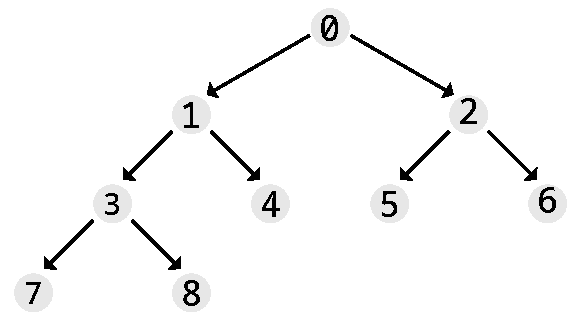
\includegraphics[scale=1]{figs/figure_heap.pdf}}
\caption{El montículo correspondiente al array que contiene los
dígitos del 0 al 8}
\label{fig.heap}
\end{figure}

Aquí presentamos una manera de construir un montículo (en 
orden alfabético parcial) desde una lista desordenada 
de letras:

\begin{verbatim}
sub construir-mont( @array, $indice is copy ) {
    my $valor-indice = @array[$indice];
    while ($indice) {
        my $padre = Int( ($indice - 1) / 2);
        my $valor-padre = @array[$padre];
        last if $valor-padre lt $valor-indice;
        @array[$indice] = $valor-padre;
        $indice = $padre;
    }
    @array[$indice] = $valor-indice;
}

sub heapify( @array ) {
    for @array.keys -> $i {
    	construir-mont @array, $i;
    }
}

my @entrada =  <m t f l s j p o b h v k n q g r i a d u e c>; 
heapify @entrada;
say @entrada;
\end{verbatim}

Nota que el montículo se construye en lugar (no hay
un necesidad para un segundo array). El array resultante
se muestra así:

\begin{verbatim}
[a b g d c k j l f h e m n q p t r o i u s v]
\end{verbatim}

¿Es este montículo correcto? Es muy difícil de saber
a primera vista y chequearlo manualmente es algo tedioso.
Al escribir un programa para construir una estructura de
datos como esta, es usualmente útil escribir algunas 
subrutinas para mostrar el contenido en un forma que 
facilite el entendimiento del resultado y el chequeo de
exactitud. El código siguiente muestras dos ejemplos
de tales subrutinas:

\begin{verbatim}
sub imprimir-mont( @array ) {
    my $inicio = 0;
    my $final = 0;
    my $último = @array.end;
    my $paso = 1;
    
    loop {
        say @array[$inicio..$final];
        last if $final == $último;
        $inicio += $paso;
        $paso *= 2;
        $final += $paso;
        $final = $último if $final > $último;
    } 
}

sub imprimir-mont2( @array ) {
    my $paso = 0;
	for @array.keys -> $actual {
	    my $h_izquierdo = @array[2 * $actual + 1];
        say "$actual\tNodo = @array[$actual];\tNo hijos" 
            and next unless defined $h_izquierdo;
        my $h_derecho = @array[2 * $actual + 2] // "' '";

        say "$actual\tNodo = @array[$actual];\tHijos: " ~ 
            " $h_izquierdo y $h_derecho";
        $paso++;
    }
}

\end{verbatim}

La primera subrutina muestra el árbol relacionado
nivel por nivel:

\begin{verbatim}
(a)
(b g)
(d c k j)
(l f h e m n q p)
(t r o i u s v)
\end{verbatim}

lo cual hace fácil dibujar el árbol (ver Figura~\ref{fig.heap2}).

\begin{figure}
\centerline
{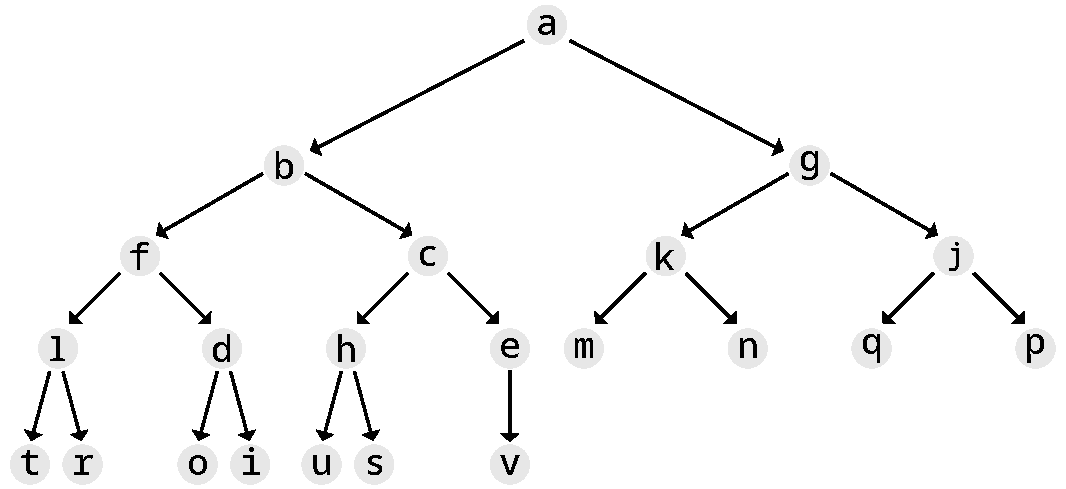
\includegraphics[scale=0.8]{figs/figure_heap2.pdf}}
\caption{El montículo correspondiente al array de letras}
\label{fig.heap2}
\end{figure}


La segunda subrutina muestra los hijos de cada nodo y hace
posible chequear fácilmente que el orden alfabético parcial
se satisface (i.e., cada nodo es menor que sus hijos):

\begin{verbatim}
0	Nodo = a;	Hijos:  b y g
1	Nodo = b;	Hijos:  d y c
2	Nodo = g;	Hijos:  k y j
3	Nodo = d;	Hijos:  l y f
4	Nodo = c;	Hijos:  h y e
5	Nodo = k;	Hijos:  m y n
6	Nodo = j;	Hijos:  q y p
7	Nodo = l;	Hijos:  t y r
8	Nodo = f;	Hijos:  o y i
9	Nodo = h;	Hijos:  u y s
10       Nodo = e;	Hijos:  v y ' '
11       Nodo = m;	No hijos
12       Nodo = n;	No hijos
(...)
21       Nodo = v;	No hijos
\end{verbatim}



\section{Depuración de Programas}
\index{debugging}

Cuando depuras un programa, y especialmente si estás 
trabajando con un error bien difícil, aquí presentamos
algunas sugerencias que podrías intentar:

\begin{description}

\item[Leer] Examina tu código, léelo, y chequea que 
diga lo que quieres decir.

\item[Ejecutar] Experimenta al hacer cambios y ejecutar las
diferentes versiones. Usualmente si muestra la cosa correcta
en el lugar correcto en el programa, el problema se vuelve 
obvio, pero algunas veces tienes que construir andamiaje para
que esto ocurra.

\item[Ejecutar con el depurador] Un {\bf depurador} es una
utilidad que te permite ejecutar un programa paso a paso,
para que puedas así seguir la ruta de ejecución y chequear
el contenido de variables importantes a puntos cruciales en
la ejecución del programa, para configurar puntos de 
interrupción, etc. Perl~6 provee un depurador, llamado 
{\tt perl6-debug}, que hace todas estas cosas posible.
Con la venida de lenguajes modernos de alto nivel, muchas
personas se resisten al uso de un depurador. Esto es un
error grave. Un depurador no te ayudará a solucionar cada 
tipo de problema, pero puede ser una utilidad inmensamente
útil. Ver la Sección~\ref{perl-debugger} para información 
adicional acerca del depurador de Perl.
\index{debugger}

\item[Reflexionar] ¡Toma tiempo para pensar! ¿Qúe tipo de error
es? ¿Sintáctico? ¿Al tiempo de ejecución? ¿Semántico?
¿Qué información puedes obtener de los mensajes de error, o desde
la salida del programa? ¿Qué tipo de error podría causar el problema
que estás observando? ¿Cuál fue el último cambio que hiciste, antes
que el problema apareciera?

\item[Depurar con el patito de goma] Si explicas el programa 
a alguien más, algunas veces encuentras la solución antes
de finalizar con la pregunta. Muy a menudo ni siquiera
necesitas la otra persona; podrías conversar con un patito
de goma. Ese es el origen de la muy conocida estrategia
conocida como la {\bf depuración del patito de goma}. 
¡Y no estoy bromeando! Lee sobre la estrategia aquí
\url{https://es.wikipedia.org/wiki/M%C3%A9todo_de_depuraci%C3%B3n_del_patito_de_goma}.
\index{rubber duck debugging}

\item[Retroceder] Algunas veces, lo mejor que puedes hacer es
retroceder, deshacer los cambios recientes, hasta que puedas
obtener un programa que funciona y que entiendas. Después puedes
comenzar la reconstrucción.

\end{description}

Los programadores principiantes algunas veces se atascan en una de
estas actividades y se olvidan de las otras. Cada actividad viene
con su propio modo de fallo.
\index{typographical error}

Por ejemplo, leer tu programa podría ayudarte si el problema es
un error tipográfico, pero no si el problema es un malentendido 
conceptual. Si no entiendes lo que tu programa hace, puedes leerlo
más 100 veces y nunca verás el error, porque el problema se encuentras en
tu cabeza.
\index{experimental debugging}


Desarrollar experimentos puede ayudarte, especialmente si ejecutas
pruebas pequeñas y simples. Pero si desarrollas experimento sin pensar 
o leer tu código, puedes caer en un patrón que llamamos ``programación de 
paso aleatorio'', el cual es el proceso de hacer cambios aleatorios hasta
que el programa haga lo correcto. Obviamente, la programación de paso aleatorio
puede tomar mucho tiempo.
\index{random walk programming}
\index{development plan!random walk programming}

Debes tomar tiempo para pensar. La depuración es como un experimento científico.
Podrías tener por lo menos una hipótesis sobre el problema (por ejemplo, 
?`cuál es el problema?). Si hay más de dos posibilidades, intenta pensar
acerca de una prueba que eliminaría uno de ellos.

Aún así, la mejores técnicas de depuración fallarán si hay muchos errores,
o si el código que estás intentando arreglar es demasiado grande y 
complicado. Algunas veces la mejor opción es retroceder, simplificar el
programa hasta que obtengas algo que funcione y que entiendas.

Los programadores principiantes son usualmente reacios a retroceder
porque no pueden tolerar el hecho de borrar una línea de código 
(aún si es algo erróneo). Si te hace sentir mejor, haz una copia de
tu programa en otro archivo antes de hacer cambios. De esa manera
puedes copiar las piezas una a la vez con cada progreso.

Encontrar un error difícil requiere leer, ejecutar (sin o con 
un depurador), reflexionar, y algunas veces retroceder. Si te atasca
en una de estas actividades, prueba las otras. 


\section{Glosario}


\begin{description}

\item[Determinista] Perteneciente a un programa que hace la misma
cosa cada vez que se ejecuta, dado la misma entrada.
\index{deterministic}

\item[Pseudoaleatorio] Perteneciente a una secuencia de números que
aparece ser aleatoria, pero es generada por un programa determinista.
\index{pseudorandom}

\item[Valor por defecto] El valor dado a un parámetro opcional si 
no se provee un argumento.
\index{default value}

\item[Sobrescribir] Reemplazar un valor por defecto con un argumento.
\index{override}

\item[Benchmarking] El proceso de elegir entre varias estructuras de datos
y algoritmos al implementar alternativas y someterlas a pruebas (
especialmente sus tiempos de duración) con una muestra de las entradas
posibles
\index{benchmarking}

\item[Depurador] Un programa que permite ejecutar un programa línea
por línea y chequea su estado a cualquier paso durante su ejecución.
\index{debugger}

\item[Depuración del patito de goma] Depuración que involucra 
explicar tu problema a un objeto inanimado tal como un patito de goma.
Articular el problema puede ayudarte a solucionarlo, aún si el patito
de goma no sabe Perl.
\index{rubber duck debugging}
\index{debugging!rubber duck}

\end{description}

\section{Ejercicio: Codificación Huffman}
\label{huffman_exercise}

La codificación Huffman es una técnica usada para la compresión de
datos, i.e., para reducir el tamaño de una pieza de datos (tal
como, por ejemplo, comprimir un archivo).

\subsection{Código de Longitud Variable}
\index{variable-length code}

Si eres familiar con el código morse, ya sabes que es un sistema
para codificar las letras del alfabeto en una serie de puntos
y rayas. Por ejemplo, la famosa señal {\tt ...---...} representa
las letras SOS, la cual constituye una llamada de ayuda reconocida
internacionalmente. La tabla en la Figura~\ref{fig.morse} 
muestra el resto de los códigos.
\index{Morse code}

\begin{figure}
\centerline
{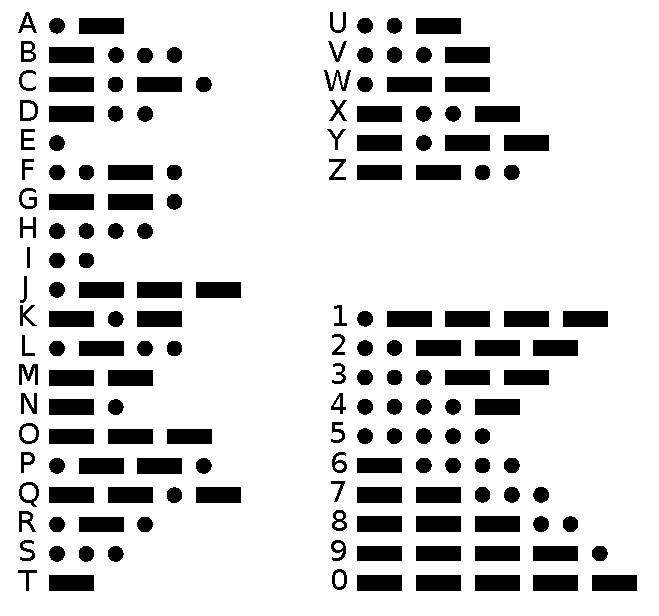
\includegraphics[scale=0.6]{figs/International_Morse_Code.pdf}}
\caption{Código Morse Internacional (dominio público)}
\label{fig.morse}
\end{figure}

El código morse (inventado entre 1836 y 1844) fue uno de los
primeros atentos de la codificación digital del alfabeto de 
un texto sencillo. El único otro atento conocido es el 
alfabeto braille (1824-1837).
\index{Morse, Samuel}
\index{braille alphabet}

Nota que algunos de los códigos son más largos que otros. Por
diseño, las letras más comunes poseen códigos más cortos. Dado
que hay un número ilimitado de códigos cortos, eso significa que
las letras y símbolos menos comunes poseen códigos más largos.
Un mensaje típico tendrás más códigos cortos que largos, lo cual
minimiza la el tiempo promedio de transmisión por letra.

Este tipo de código se conoce como códigos de longitud variable. 
En este ejercicio, estudiaremos un algoritmo para generar código
de longitud variable llamado codificación Huffman. Es un algoritmo
interesante en sí mismo, pero también hace de un ejercicio interesante
porque su implementación usa una variedad de estructuras de datos.
\index{Huffman!code}

Aquí presentamos un esquema de lo que haremos hasta al final de este capítulo:

\begin{enumerate}

\item Primeramente, usaremos una muestra de texto en inglés para generar
un tabla de los caracteres y sus frecuencias.

\item Después usaremos esta tabla de frecuencia para generar una tabla
de código.

\item Finalmente, codificaremos un mensaje con esta tabla de código y 
consiguientemente lo decodificaremos.

\end{enumerate}

\subsection{La Tabla de Frecuencias}
\index{frequency!table}

Dado que la meta es proveer las letras comunes con códigos
cortos, necesitamos saber la frecuencia con la cual cada letra
ocurre. En la historia ``The Gold Bug``\footnote{El Escarabajo de Oro} 
de Edgar Allan Poe, uno de los personajes, William~Legrand, 
usa la frecuencia de las letras para descifrar un criptograma. Él explica: 
\index{Poe, Edgar Allan}
\index{The Gold-Bug (Edgar Allan Poe)}
\index{cypher}

\begin{quote}
``Now, in English, the letter which most frequently occurs 
is e. Afterwards, the succession runs thus: a o i d h n r s 
t u y c f g l m w b k p q x z. E however predominates so 
remarkably that an individual sentence of any length is 
rarely seen, in which it is not the prevailing character.''
\footnote{
``
Ahora bien: la letra que se encuentra con mayor frecuencia en inglés es la 
e. Después, la serie es la  siguiente: a o y d h n r s t u y c f g l m w b k p q x z. 
La e predomina de un modo tan notable, que es raro encontrar una frase sola de
cierta longitud de la que no sea el carácter principal.``}
\end{quote}

Nuestra misión es chequear si Poe estaba en lo cierto. Para chequearlo,
usaremos una muestra del texto del ``The Gold Bug``, el cual
puede descargarse desde le Proyecto Gutenberg
(\url{http://www.gutenberg.org/files/2147/2147-0.txt}) 
y una variedad de otros sitios web.
\index{Project Gutenberg}

\begin{exercise}
\label{letter_frequency}
Escribe un programa que cuenta el número de veces que cada letra 
aparece en una muestra de texto. Descarga el texto de ``The Gold Bug'' 
y analiza la frecuencia de las letras.

Solución: ver Sección~\ref{sol_letter_frequency}
\end{exercise}

\subsection{Construyendo el Código Huffman}
\index{Huffman!code}

Para nuestro propósito, el código morse tiene un defecto: 
no solamente usa dos símbolos como podrías pensar, sino
que actualmente usa tres: además de los puntos y las rayas,
también usa el espacio entre los dos símbolos implícitamente,
como también espacios más largos entre dos letras.
\index{Morse code}

La razón por la cual algunos espacios son necesarios es muy simple.
Usa la tabla de código morse anterior y supón que recibes 
tres puntos (\verb'...'). Esto podría ser interpretado como la letra
``e`` tres veces, o como ``ie`` o ``ei`` o como ``s``, o como el
inicio de ``h``, ``v``, ``3``, ``4``, o ``5``. Los espacios agregados 
hacen posible distinguir entre las varias posibilidades. Pero
también hacen la transmisión de código mucho más lenta.

En 1951, David A. Huffman inventó una técnica de construcción de código
que evita este problema: provisto que sepas donde una letra dada 
comienza, no existe ninguna ambigüedad. Por ejemplo, trabajaremos 
más tarde con un código Huffman para un subconjunto pequeño
del alfabeto que luce así:
\index{Huffman, David A.}
\index{Huffman!code}

\begin{verbatim}
a => ..
e => .-
s => -.-
n => -..
t => --.
d => ---.
r => ----
\end{verbatim}

Si comienzas a leer una secuencia de puntos y rayas que representan
un texto válido compuesto con estas sietes letras, siempre puedes
decodificarlo sin ninguna ambigüedad. Si el primer símbolo es 
un punto, entonces la letra es una ``a`` o un ``e`` dependiendo 
en el símbolo siguiente. Si el primer símbolo es una raya y 
el siguiente es un punto, entonces la letra deber ser una ``s`` o
una ``n`` dependiendo del tercer símbolo. Si los primeros símbolos
son rayas, puedes similarmente determinar que la letra actual es una
``t`` (si el tercer símbolo es un punto), o una ``d`` o una ``r``. 
la cual puedes encontrar al revisar el cuarto símbolo. En resumen, 
no necesitas espacios entre los símbolos, siempre es posible
decodificar una letra sin ambigüedad.

¿Cómo podemos construir un código Huffman? Hagámoslo manualmente con
un alfabeto bien simple: las cuatros letras de las bases nitrogenadas
del ADN: A, C, T y G. Supón que queremos codificar la siguiente
cadena de texto de entrada:
\index{DNA (deoxyribonucleic acid)}
\index{alphabet}

\begin{verbatim}
CCTATCCTCGACTCCAGTCCA
\end{verbatim}

Esto resulta en la tabla de frecuencia siguiente:
\index{frequency!table}

\begin{verbatim}
C :     10      47.62
T :     5       23.81
A :     4       19.05
G :     2        9.52
\end{verbatim}

Para construir el código Huffman, comenzamos con las dos letras
menos frecuentes y las mezclamos en un símbolo nuevo temporario, 
\verb|[GA]|, el cual pretendemos es una letra compuesta nueva con una
frecuencia  de 6. En este punto, decidimos que, entre dos letras,
a la menos frecuente se le adjuntará un punto y a la otra se le
adjuntará una raya (este es una decisión arbitraria, podría
hacerse de la manera inversa). Así que decimos que el símbolo 
para la letra menos común de las dos letras (``G``) será \verb|[GA].|
y \verb|[GA]-| será el símbolo para la ``A``. 

Ahora tenemos tres letras, C, T, and [GA]. Mezclamos las dos letras
menos frecuente, ``T'' y ``[GA],'' y podemos ahora decir que el
símbolo para la ``T'' será \verb|[TGA].| y el símbolo para \verb|[GA]|
será \verb|[TGA]-|. Ahora tenemos solo dos letras restantes, 
``C'' and ``TGA``, con ``C'' siendo la menos frecuente; así que 
``C'' será un punto y ``TGA`` será una raya.

We can now unroll our dummy letters: ``T'' es \verb|[TGA].|, 
así que, reemplazando \verb|[TGA]| con su símbolo, i.e., una raya,
el código final para ``T`` será \verb|-.|; similarmente, \verb|[GA].|
ahora puede traducirse como \verb|--|. Por el mismo proceso de
sustitución, podemos ahora determinar que ``A`` es \verb|---| y ``G``
es \verb|--.|. Así que nuestra tabla final de código Huffman:
\index{Huffman!table}

\begin{verbatim}
C => .
T => -.
G => --.
A => ---
\end{verbatim}

Nota que, debido a la construcción, la letra más frecuente (C)
tiene el código más corto mientras que las letras menos
comunes (G y A) tienen los códigos más largos.

La codificación manual de cadena de texto de entrada 
\verb|CCTATCCTCGACTCCAGTCCA| con este código rinde el 
código pseudo-Morse siguiente:
\index{pseudo-Morse}

\begin{verbatim}
..-.----...-..--.---.-...-----.-...---
\end{verbatim}

Nota que nuestro código Huffman no tiene ambigüedad:
el primer punto puede solo ser una ``C``, y el segundo también.
El símbolo siguiente es una raya, que puede ser el inicio de 
las otras tres letras, pero solo la	 ``T`` puede tener un punto 
posterior. La secuencia siguiente de símbolos tiene cuatro 
rayas; esto puede solamente tres rayas de una ``A``, con la 
última raya siendo el inicio de la letra siguiente; y \verb|-.|
solo puede ser una ``T``, etc.
\index{Huffman!code}

En una codificación de Huffman real para la compresión de
archivos de texto, no usaríamos puntos y rayas, pero los 
bits 0 y 1; sin embargo, los punto y las rayas son solo
otra manera conveniente de representar esos valores
binarios. Por lo tanto, pretendamos que los puntos y las
rayas son realmente los números binarios 0 y 1.
\index{binary number}
\index{bit}

\index{data compression}
¿Realmente logramos la compresión de datos? Nuestra cadena
de pseudo-Morse tiene 38~símbolos binarios. La cadena de 
texto de entrada original tenía 21 caracteres o bytes, eso 
son 168~bits. Los datos han sido comprimidos por un factor
de 4.4. 
\index{byte}

¿Es la codificación de Huffman mejor que la codificación de 
longitud fija? Una representación de una cadena de texto donde
cada letra sería representada por dos bits (dos bits pueden
representar cuatros letras) requiere 42~símbolos. Por lo tanto,
sí, obtuvimos una mejor compresión de datos que una codificación
de longitud fija (alrededor de 10\%). Este puede parecer un logro
minúsculo, pero es actualmente un gran logro con un alfabeto tan
pequeño. Con datos textuales actuales, la codificación de Huffman
puede lograr una significante compresión de datos.


\begin{exercise}
\label{huffman_code_2}
\begin{enumerate}

\item Escribe un programa que realiza codificación de Huffman
de una cadena de texto de caracteres simple. Puedes comenzar con
el ejemplo de ADN más arriba. No te preocupes si no obtienes la
misma tabla de Huffman de más arriba: pueden haber más código
de Huffman para una cadena de texto dada; pero chequea que obtengas
un código que no sea ambiguo.
\index{Huffman!code}

\item Haz una prueba con cadenas de texto que tienen un alfabeto
más grande (probablemente querrás comenzar con un alfabeto
relativamente pequeño porque, por lo contrario,
puede ser tedioso chequear el resultado manualmente).
 
\item Escribe una subrutina que codifique una cadena de texto
de entrada en pseudo-Morse usando la tabla de Huffman generada
anteriormente.
\index{pseudo-Morse}
\index{alphabet}

\item Escribe una subrutina que decodifique la salida pseudo-Morse
que has generado para la pregunta anterior.
\end{enumerate}
%
Solución: ver Sección~\ref{sol_huffman_code_2}.
\index{Huffman!code}
\end{exercise}




\part{Hacia Adelante}

% intro_part_2.tex -- Introduction to second part
%
% \chapter{Introduction to the Second part of this book}

Ahora que has alcanzado el final de la primera parte 
de este libro, ya no deberías sentirte un principiante.
Ahora, deberías ser capaz de leer (y escudriñar) la 
documentación oficial de Perl~6 (\url{https://docs.perl6.org})
y encontrar tu camino.

Hay muchas cosas que decir acerca de la programación.
Los siguientes tres capítulos se dedicaran a conceptos
más avanzados y a nuevos paradigmas de programación,
incluyendo:
\begin{description}

\item[Programación Orientada a Objetos] Describiremos 
cómo construir nuestros propios tipos y métodos, lo cual
es una manera de extender el lenguaje.

\item[Uso de gramáticas] Esta es una forma de programación
declarativa en la cual defines axiomas y reglas y derivas
conocimientos de estos; las gramáticas son una forma muy
poderosa de analizar contenido textual y se usan para 
transformar el código fuente de un programa en sentencias
que se pueden ejecutar.

\item[Programación funcional] Este es aún otro tipo de paradigma 
de programación en el cual una computación se expresa como
la evaluación de funciones matemáticas.
\end{description}

Cada uno de estos capítulos probablemente merece un
libro completo (y podrían tener uno en el futuro) 
pero esperamos decirte lo suficiente acerca
de ellos para ponerte en marcha. En mi opinión,
cada programador debería saber sobre estos conceptos 
poderosos para ser capaz de seleccionar la mejor forma
de resolver un problema en particular.

Perl~6 es un lenguaje multiparadigmático, así que 
podemos cubrir estas disciplinas usando el lenguaje Perl~6.
Un número de temas que introducimos en los
capítulos anteriores deberían facilitar la fácil
adquisición de estas nuevas ideas, y esta es la 
razón por la cual pienso que es posible cubrirlas
apropiadamente solo con un capítulo para cada una de
estas disciplinas.

Habrán menos ejercicios en la segunda parte, 
porque esperamos por ahora que ya eres capaz de idear 
tus propios ejercicios y hacer tus propios experimentos.
Y habrán solo algunas soluciones sugeridas, porque 
nos estamos acercando a un nivel donde no existe una 
única solución correcta, sino muchas maneras de 
enfrentar y resolver un problema.

Con respecto al lenguaje Perl, hemos cubierto muchísimo 
material, pero, como te advertí al principio, estos
estos dista de ser exhaustivo. Los siguientes son los temas
que no cubrimos (y no cubriremos); podrías desear explorar
la documentación por ti mismo:

\begin{description}
\item[Programación concurrente] Las computadoras de hoy en día
poseen procesadores múltiples o procesadores con múltiples
núcleos; Perl~6 ofrece varias formas de tomar ventaja de estos
para ejecutar procesos de computación en paralelo para así 
mejorar el rendimiento y reducir el tiempo de ejecución; ver
\url{https://docs.perl6.org/language/concurrency} 
for more details.

\item[Manejo de excepciones] El manejo de situaciones
cuando algo no funciona correctamente es una parte 
importante de la programación. Perl~6 ofrece varios
mecanismos para el manejo de tales situaciones.
Ver \url{https://docs.perl6.org/language/exceptions} 
para más detalles.

\item[Comunicación entre procesos:] Programas usualmente tienen
que ejecutar otros programas y comunicarse con los mismos. Ver 
\url{https://docs.perl6.org/language/ipc}.

\item[Módulos] Cómo crear, usar, y distribuir módulos de
Perl~6. Ver \url{https://docs.perl6.org/language/modules}.

\item[Intefaz para llamadas nativas] Cómo llamar librerías que están
escritas en otros lenguajes de programación y seguir las
convenciones de llamadas del lenguaje C.
Ver \url{https://docs.perl6.org/language/nativecall}

\end{description}

\chapter{Clases y Objetos}
\label{objects}
\index{object}
\index{class}

A esta altura ya sabes cómo usar funciones para organizar código
y tipos integrados para organizar datos. El siguiente paso es aprender
``programación orientada a objetos,`` la cual usa tipos definidos por
el programador para organizar código y datos.
\index{abstraction}
\index{encapsulation}

Cuando las aplicaciones de software comienzan a crecer, el número
de detalles que se debe manejar puede volverse agobiante. La única 
manera de manejar esta complejidad es usar abstracción y encapsulamiento.
La programación orientada a objetos es una manera muy popular y eficiente
de implementar abstracción y encapsulamiento. 

Perl~6 es un {\bf lenguaje de programación orientado a objetos}, lo cual significa
que el lenguaje provee características que soportan la
programación orientada a objetos, la cual posee las siguientes
características definitivas:
\index{object-oriented programming}

\begin{itemize}

\item Los programas incluyen definiciones de clases y métodos.
\index{class}
\index{method}

\item La mayor parte de la computación se expresa en términos de 
operaciones sobre los objetos.

\item Los objetos usualmente representan cosas en el mundo real, y los 
métodos normalmente corresponden a las formas de interacción de las
cosas en el mundo real.
\end{itemize}

La programación orientada a objetos en Perl~6 es un tema enorme que 
merece un libro para sí mismo (y probablemente habrá un libro o dos sobre la
materia en algún punto). Este capítulo hará más que analizar el
tema superficialmente y te permitará crear y usar objetos. Sin embargo,
no cubrirá algunos detalles y características más avanzadas.
\index{OOP (object-oriented programming)}
\index{object-oriented programming (OOP)}

\section{Objetos, Métodos y Programación Orientada a Objetos}
\index{object-oriented programming (OOP)}
\index{programming!object-oriented}

Empecemos con una sinopsis general de la programación orientada a objetos
y una breve introducción a la jerga asociada con la misma.


\index{object}
En la ciencia de la computación, un objeto puede describirse 
vagamente como una dirección de memoria o una entidad que 
posee un valor, y su usualmente es conocido como un identificador.
Esto puede ser una variable, una estructura de datos, un array,
o posiblemente hasta una función. No usaremos esta concepción
general con el mismo sentido en este capítulo.

En la programación orientada a objetos (POO), la palabra
{\bf objeto} tiene un significado mucho más específico: un 
objeto es una identidad que usualmente tiene:
\begin{itemize}

\item Una identidad (por ejemplo, su nombre).

\index{object! behavior}
\item Algunas propiedades que definen su comportamiento (en la forma
de funciones especiales que son comúnmente conocidas como {\bf métodos});
este comportamiento usualmente no cambia con el tiempo y es 
generalmente común a todos los objetos del mismo tipo.
\index{method}

\item Un {\bf estado} el cual es definido por algunas variables
especiales (conocidas como, dependiendo en el lenguaje, atributos,
campos, o miembros); el estado puede cambiar a medida que pasa el 
tiempo y es generalmente específico a cada objeto. En Perl, nos
referimos a dichas variables como {\tt atributos}.
\index{object!state}
\index{object!attribute}
\index{attribute!object}
\end{itemize}

En resumen, un objeto es un conjunto de atributos y métodos
todos juntos.

\index{class}
Los objetos son usualmente definidos dentro de un tipo
de paquete de código conocido como una {\bf clase}. 
Una clase define los métodos y la naturaleza de los
atributos asociados a un objeto. En Perl~6, una clase
hace posible definir nuevos tipos similares a los tipos
integrados que hemos visto hasta ahora. Muy pronto comenzaremos
a definir algunas clases y las usaremos para crear objetos.
\index{type!building new type}

\index{invocant}
\index{method}
\index{dot notation}
Ya sabes informalmente lo qué es un método, dado que hemos
usado métodos integrados a lo largo del libro. Es como una 
como una función con una sintaxis sufija que usa la notación
del punto sobre el invocante. Por ejemplo, puedes invocar el
método {\tt say} sobre una simple cadena de texto:

\begin{lstlisting}
"foo".say;           # -> foo
\end{lstlisting}

Nota que ``foo'' no es un objeto, pero una simple cadena de texto.
No obstante, puedes invocar el método \verb|say| sobre la misma,
debido a que Perl puede tratarla internamente como un objeto cuando
es necesario. En algunos otros lenguajes POO, esta conversión implícita
de un tipo nativo a un objeto es conocida como autoboxing.
\index{autoboxing}

Probablemente recuerdas que los métodos pueden ser encadenados
en un proceso donde el valor devuelto por un método se convierte
en el invocante para el siguiente método:

\begin{lstlisting}
"foo".uc.say;        # -> FOO

my @alfabeto = <charlie foxtrot alpha golf echo bravo delta>;
@alfabeto.sort.uc.say;
    # imprime: ALPHA BRAVO CHARLIE DELTA ECHO FOXTROT GOLF 
\end{lstlisting}

\index{role}
En POO, los métodos que se pueden aplicar a los objetos son
usualmente definidos dentro de las clases, regularmente
la clase que también definió el objeto o alguna otra clase 
con una cercana relación. En Perl~6, los métodos pueden también
ser definidos en un {\bf role}, el cual es otro tipo de 
paquete de código que se parece a una clase, como veremos
más adelante.

\index{black box}
\index{encapsulation}
La idea básica de la programación orientada a objetos es
que un objeto es un tipo de caja negra que oculta su
estructura interna (datos y código) del usuario; el usuario
puede consultar o cambiar el estado de un objeto a través de
los métodos. El proceso de ocultar la estructura interna
de los objetos se conoce como {\bf encapsulación}. Esto usualmente
permite tener una perspectiva más general y una mejor abstracción
de datos con respecto a lo que hemos visto hasta ahora;
esto resulta en programas con menos errores (especialmente programas
extensos).

En adición, POO usualmente ofrece los siguientes conceptos:
\begin{itemize}
\index{polymorphism}
\item {\bf polimorfismo}, i.e., la función o el método tiene la
posibilidad de hacer cosas diferentes dependiendo del tipo de 
objeto que la llama o lo invoca;
\index{inheritance}
\item {\bf herencia}, i.e., la posibilidad de derivar una clase de
otra clase, de tal manera que la clase hija hereda algunas de la 
propiedades de la clase {\bf padre}, la cual es una herramienta
poderosa para el reutilización de código.
\end{itemize}

Ahora estudiaremos cómo todo estos conceptos se implementan en Perl.


\section{Tipos Definidos por el Programador}
\label{point}
\index{programmer-defined type}
\index{type!programmer-defined}

Hemos usado muchos tipos integrados de Perl; ahora vamos
a definir un nuevo tipo. Como un ejemplo, crearemos un
tipo llamado {\tt Punto2D} que representa a un punto en
el espacio bidimensional.
\index{point, mathematical}
\index{two-dimensional space}

En notación matemática, los puntos son usualmente escritos
en paréntesis con una coma que separa las coordenadas.  Por 
ejemplo, en las coordenadas cartesianas o rectangulares,
$(0,0)$ representa el origen, y $(x,y)$ representa un punto
$x$ unidades a la derecha y $y$ unidades a la izquierda. $x$
se llama la abscisa y $y$ la ordenada.
\index{Cartesian coordinates}
\index{coordinates!Cartesian}
\index{coordinates!rectangular}
\index{rectangular coordinates}

Hay varias maneras de representar un punto en Perl:

\begin{itemize}

\item Podemos almacenar las coordenadas separadamente 
en dos variables, {\tt \$x} y {\tt \$y}.

\item De igual manera, podemos almacenar las coordenadas como
elementos en una lista, un array, o una pareja.

\item Así mismo, podemos crear un nuevo tipo que representa
puntos como objetos.

\end{itemize}
\index{representation}

Crear un nuevo tipo es un poco más complicado que las otras
opciones, pero tiene ventajas que serán aparentes muy pronto.

Un tipo definido por el programador es usualmente creado con 
una {\bf clase} (o un {\bf rol}, pero regresaremos a esto más tarde).
La definición de una clase bien simple para un tipo que representa a 
un punto luce así:
\index{class}
\index{object!class}
\index{class!definition}
\index{definition!class}
\index{role}
\index{Point2D class}

\begin{lstlisting}
class Punto2D {
    has $.abscisa;               # valor "x"
    has $.ordenada;              # valor "y" 
}
\end{lstlisting}
%
La cabecera indica que la nueva clase se llama {\tt Punto2D}. 
El cuerpo define dos atributos, i.e., propiedades con nombres
asociadas con la clase, aquí la abscisa y la ordenada 
(o las coordenadas $x$ y $y$) del punto.
\index{Point2D class}
\index{class!Point2D}

\index{type object}
La definición de una clase con el nombre {\tt Punto2D} crea
un {\bf tipo objeto}.

El tipo objeto es como una factoría para crear objetos. Para crear
un punto, tú llamas el método {\tt new} sobre la clase {\tt Punto2D}:

\begin{lstlisting}
my $punto = Punto2D.new( 
    abscisa  => 3, 
    ordenada => 4
);
say $punto.WHAT;                # -> (Point2D)
say $punto.isa(Punto2D)         # -> True
say $punto.abscisa;             # -> 3
\end{lstlisting}
%
\index{isa method}
\index{WHAT}
Por supuesto puedes crear tanto puntos como desees.

\index{constructor}
\index{new, object constructor}
\index{dot notation}
\index{object!constructor}
El método {\tt new} se llama un {\bf constructor} y no se ha 
definido en este ejemplo; esto no es necesario dado que 
Perl~6 provee un constructor {\tt new} por defecto para 
cada clase (como veremos más adelante). La sintaxis de invocación
de método, con la notación de punto, es la misma que hemos 
usados a lo largo del libro para invocar los métodos integrados.
No estás forzado a usar este constructor; también puedes crear
tu propio constructor (y puedes nombrarlo {\tt new o algo diferente}),
pero usaremos el método integrado {\tt new} por el momento.
\index{invocation!method}
\index{method invocation}

El proceso de crear un nuevo objecto con una clase es conocido
como {\bf instanciación}, y el objeto es una {\bf instancia} de la
clase.
\index{instance}
\index{object!instance}
\index{instantiation}

Cada objeto es una instancia de alguna clase, 
así que los términos ``objeto`` e ``instancia`` son
intercambiables. Pero usualmente usaremos ``instancia``
para indicar que estamos hablando de un objeto que pertenece
a un tipo definido por el programador.
\index{type}
\index{programmer-defined type}

\section{Atributos}
\label{attributes}
\index{instance attribute}
\index{attribute!instance}
\index{dot notation}

Los atributos que hemos definido son las propiedades asociadas
con las clase {\tt Punto2D} pero, al mismo tiempo, son específicas
a la instancia de la clase que hayamos creado. Ellos son los
atributos de la instancia. Si creamos otro objeto {\tt Punto2D},
también tendrá los mismos atributos, pero los valores de tales
atributos serán probablemente diferentes. 

La figura~\ref{fig.point2d} muestra el resultado de estas asignaciones.
Un diagrama de estado que muestra un objeto y sus atributos es conocido
como un {\bf diagrama de objeto}.
\index{state diagram}
\index{diagram!state}
\index{object diagram}
\index{diagram!object}

\begin{figure}
\centerline
{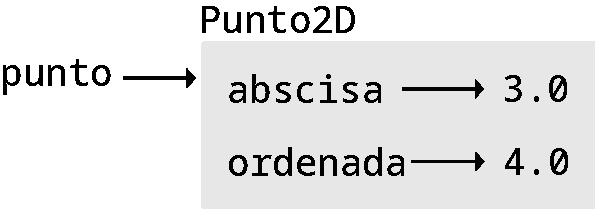
\includegraphics[scale=0.8]{figs/point2D.pdf}}
\caption{Diagrama de objeto.}
\label{fig.point2d}
\end{figure}

La variable {\tt \$punto} se refiere a un objeto {\tt Punto2D},
el cual contiene dos atributos. 

Cada atributo de la clase {\tt Punto2D} debe referirse a un 
número, pero esto no es obvio en la definición actual de la clase.
Al momento podemos crear un objeto {\tt Punto2D} con un cadena de texto
como la abscisa, lo cual no hace sentido. Podemos mejora la definición de
la clase al especificar un tipo numérico para los atributos:
%
\begin{lstlisting}
class Punto2D {
	has Numeric $.abscisa;               # valor "x"
	has Numeroc $.ordenada;              # valor "y" 
}
\end{lstlisting}
%
\index{private attribute}
\index{attribute!private}
Los atributos de la instancia son privados para la clase,
lo cual significa que no puede accederse fuera de la clase:
usualmente necesitarías invocar un método de la clase (i.e., un
tipo de subrutina definida dentro de la clase), para obtener su
valor. No obstante, cuando se define un atributo con un punto como 
en \verb|$.abscisa|:

\begin{lstlisting}
    has $.abscisa;  
\end{lstlisting}
%
\index{accessor}
\index{method!accessor}
Perl crea un método implícito \emph{de acceso}, i.e., un método
que comparte el nombre del atributo y devuelve el valor de dicho
atributo. Así que, cuando escribimos:

\begin{lstlisting}
say $punto.abscisa;                     # -> 3
\end{lstlisting}
%
no estábamos accediendo el atributo {\tt abscisa} del objeto
\verb|$punto| directamente, sino que estábamos llamando al método
{\tt abscisa} sobre el objeto, el cual devolvió el valor de ese
atributo.

\index{dot notation}
\index{accessor}

Puedes usar dicho un método de acceso con la notación de punto
como parte de cualquier expresión. Por ejemplo:

\begin{lstlisting}
my $dist-al-centro = sqrt($punto.abscisa ** 2 + $punto.ordenada ** 2);
\end{lstlisting}
%

También hay otra manera de declarar un atributo en una clase, 
usando el twigil de signo de exclamación en vez de un punto:
\index{twigil}

\begin{lstlisting}
    has $!abscisa;  
\end{lstlisting}
%
\index{attribute!private}
\index{private attribute}
En ese caso, Perl no crea un método implícito de acceso 
y el atributo solo se puede acceder desde otros métodos
dentro de la clase. Tal atributo es ahora completamente privado. 
Sin embargo, si declaras atributos de esta manera, no podrás
asignarles ningún valor durante la creación del objeto con el 
constructor por defecto {\tt new} y necesitarás crear tu propio
constructor (or modificar {\tt new} indirectamente). Así que no
intentes esto por el tiempo presente, dado que no serás capaz
de hacer mucho con tus objetos en este punto. Regresaremos a esto 
más tarde.

\index{attribute!mutable}
\index{attribute!immutable}
Por defecto, los atributos de un objeto no son mutables; solo
se pueden leer. Esto significa que no puedes modificarlos una vez que 
se ha creado el objeto. Esto funciona bien para algunos atributos: si
un objeto representa a una persona, es poco probable que el nombre 
de la persona y su fecha de nacimiento cambien. Otros atributos necesitan
ser actualizados, muchas veces muy frecuentemente. En tales casos, los
atributos pueden declararse como mutables con el rasgo (del inglés \emph{trait})
 {\tt is rw}:
\index{is rw trait}
\index{trait!is rw}

\begin{lstlisting}
class Punto2D {
	has Numeric $.abscisa is rw;               # valor "x"
	has Numeroc $.ordenada is rw;              # valor "y" 
}
\end{lstlisting}
%
Ahora es posible modificar estos atributos. Por ejemplo,
podemos cambiar la abscisa del punto recién creado:

\begin{lstlisting}
# Primero creamos un objeto Punto2D:
my $punto = Punto2D.new(abscisa => 3, ordenada => 4);
say $punto;    # -> Punto2D.new(abscisa => 3, ordenada => 4)

# Ahora movemos el objeto $punto dos unidades a la derecha:
$punto.abscisa = 5; 
say $punto;    # -> Punto2D.new(abscisa => 5, ordenada => 4)
\end{lstlisting}


\index{class!attribute}
\index{attribute!class}
Casi toda la información presentada aquí acerca de los atributos
está relacionada con los atributos de la instancia, i.e., propiedades
relacionada a objetos individuales. También puedes tener atributos que
pertenecen a la clase entera, los cuales se conocen como \emph{atributos de la
clase}. Son menos común que los atributos de una instancia y son declarados
con el declarador {\tt my} (en vez de {\tt has}). Un ejemplo típico de
una atributo de una clase sería un contador al nivel de la clase para
mantener un récord del número de objetos que se han instanciado.


\section{Creando Métodos}
\index{method}

La simple clase {\tt Punto2D} y su instancia \verb|$punto|
no son muy útil al momento. Completemos la definición de la
clase con algunos métodos:
\index{Point2D class}

\begin{lstlisting}
class Punto2D {
    has Numeric $.abscisa;
    has Numeric $.ordenada;
    
    method coordenadas {        #  método de acceso para "x" y "y"
        return (self.abscisa, self.ordenada)
    }
    
    method distancia-al-centro {
        (self.abscisa ** 2 + self.ordenada ** 2) ** 0.5
    }
    method coordenadas-polares {
        my $radio = self.distancia-al-centro;
        my $theta = atan2 self.ordenada, self.abscisa;
        return $radio, $theta;
    }
}
\end{lstlisting}

Aquí declaramos tres métodos en la clase:
\begin{itemize}
\item {\tt coordenadas}, un simple método de acceso a
las coordenadas cartesianas;
\index{coordinates!Cartesian}
\index{Cartesian coordinates}

\item{\tt distancia-al-centro}, un método que calcula y devuelve
la distancia entre el objeto y el origen;

\index{polar coordinates}
\index{coordinates!polar}
\item{\tt coordenadas-polares}, un método que calcula el radio y 
el azimuth (\verb|$theta|) del objeto en el sistema de coordenada
polar (nota que {\tt coordenadas-polares} invoca al método 
{\tt distancia-al-centro} para encontrar el componente radio de las 
coordenadas polares).
\end{itemize}

\index{invocant}
La definición de un método no es muy distinta a la definición
de una subrutina, excepto que usa la palabra clave {\tt method}
en vez de {\tt sub}. Esto no es una sorpresa dado que un 
método es esencialmente una subrutina que se define dentro de
una clase (o un rol) y sabe acerca de su \emph{invocante}, i.e.,
el objeto que lo llama y su clase. Y, por supuesto, tiene una
sintaxis de llamada diferente.
\index{method}

\index{method!dispatch}
\index{dispatching methods}
\index{invocation!method}
\index{method invocation}
Otra diferencia importante entre una subrutina y un método es
que, debido a que hay varios métodos con el mismo nombre
definidos en diferentes clases (o diferentes roles), una 
invocación de método conlleva un fase de \emph{despacho},
en la cual el sistema de objeto selecciona cuál método llamar,
usualmente basado en la clase o tipo del invocante. Sin embargo,
en Perl~6, esa diferencia no es muy clara por hecho de que 
puedes tener multi subrutinas, i.e., subrutinas con el mismo
y una signatura diferente que son resueltas al tiempo de ejecución,
dependiendo en la \emph{aridad} (número de argumentos) y el 
tipo de los argumentos.
\index{arity}
\index{type}

Dentro de la definición de un método, {\tt self}
se refiere al \emph{invocante}, el objeto que invocó
al método. Existe un atajo para el mismo, \verb|$.|,
así que podríamos escribir el método {\tt coordenadas}
de la siguiente manera:
\index{self}

\begin{lstlisting}
    method coordenadas {        #  método de acceso para "x" y "y"
        return ($.abscisa, $.ordenada)
    }
\end{lstlisting}

Los dos formatos de sintaxis, \verb|$.| y {\tt self}, son
esencialmente equivalentes.

Existe una tercera manera de lograr el mismo objetivo,
la cual usa el signo de exclamación en vez del punto:

\begin{lstlisting}
    method coordenadas {        #  método de acceso para "x" y "y"
		return ($!abscisa, $!ordenada)
	}
\end{lstlisting}

Aquí, el resultado sería el mismo, pero esta nueva sintaxis
no es equivalente: \verb|$.abscisa| es una invocación de método,
mientras que \verb|$!abscisa| provee acceso directo al atributo. 
La diferencia es que \verb|$!abscisa| está disponible dentro de 
la clase (y podría ser un poco más rápida), mientras
la sintaxis de invocación de método puede ser usada en cualquier
otra parte (por ejemplo dentro de otra clase). Veremos en la 
siguiente sección ejemplos de esta distinción y sus consecuencias.
\index{invocation!method}
\index{method invocation}

Podemos ahora crear un objeto e invocar nuestros métodos:

\begin{lstlisting}
my $punto =  Punto2D.new(
    abscisa => 4, 
    ordenada => 3
);
say $punto.coordenadas;            # -> (4 3)
say $punto.distancia-al-centro;    # -> 5
say $punto.coordenadas-polares;    # -> (5 0.643501108793284)
\end{lstlisting}

\index{topical variable}
\index{invocant}
Podría ser que recuerdes que si usas un método sin nombrar el
invocante explícitamente, entonces el método se aplica
a la \verb|variable tópico|:

\begin{lstlisting}
.say for <one two three>;       # -> one two three (cada uno en su propia línea)
\end{lstlisting}

\index{for loop}
\index{given statement}
Ahora que hemos creado un objeto con algunos métodos, también
podemos tomar ventaja de la misma sintaxis. Por ejemplo, si 
usamos {\tt for} o {\tt given} para poblar la variable tópico
\verb|$_| con el objeto \verb|$punto|, podemos escribir:

\begin{lstlisting}
given $punto {
    say .coordenadas;             # -> (4 3)                       
    say .distancia-al-centro;     # -> 5                 
    .coordenadas-polares.say;     # -> (5 0.643501108793284)
}    
\end{lstlisting}

Como ejercicio, podrías escribir una subrutina llamado 
\verb|distancia-entre-puntos| que toma dos puntos
como argumentos y devuelve la distancia entre ellos 
usando el teorema de Teorema de Pitágoras.

Los métodos de nuestra clase son todos métodos de acceso,
lo cual significa que ellos proveen el estado de algunos de los atributos
del invocante. Si los atributos son mutable (al ser declarados con
con el trait \verb|is rw|), podemos también creamos algunos \emph{mutadores},
i.e., métodos que se invocan para cambiar aquellos atributos mutables:
\index{accessor}
\index{mutator}

\begin{lstlisting}
class Punto2D-mutable {
    has Numeric $.abscisa is rw;
    has Numeric $.ordenada is rw;
    
    # quizás los mismos métodos de acceso como
    # en la clase anterior.
    
    method nueva-ordenada (Numeric $ord) {
        self.ordenada= $ord; 
    }
}
# Creando un objeto Punto2D-mutable:
my $punto = Punto2D-mutable.new(abscisa => 3, ordenada => 4);
say $punto;  # -> Punto2D-mutable.new(abscisa => 3, ordenada => 4)

# Modificando la ordenada:
$punto.nueva-ordenada(6);
say $punto;  # -> Punto2D-mutable.new(abscisa => 3, ordenada => 6)
\end{lstlisting}




\section{Rectángulos y Composición de Objetos}
\label{rectangles}
\index{rectangle}
\index{composition!object}
\index{object!composition}

Algunas veces es obvio qué los atributos de un objeto deberían ser,
pero otras veces debes hacer decisiones. Por ejemplo, imagínate que estás
diseñando una clase para representar rectángulos. ?`Qué atributos usarías para
especificar la ubicación y tamaño de un rectángulo? Puedes ignorar 
los ángulos; para mantener las cosas simples, asume que los bordes 
del rectángulo son verticales or horizontales.
\index{representation}

Existen por lo menos dos posibilidades:

\begin{itemize}

\item Podrías especificar una esquina del rectángulo (o el centro), 
el ancho, y la altura.

\item Podrías dos esquinas opuestas.

\end{itemize}

En este momento es difícil decir cuál de las opciones es mejor, 
así que implementaremos la primera, como un ejemplo.
\index{Rectangle class}
\index{class!Rectangle}

Aquí está la definición de la clase:

\begin{lstlisting}
class Rectángulo {
    has Numeric $.ancho;
    has Numeric $.altura;
    has Punto2D $.esquina;     # vértice inferior izquierdo 

    method area { return $.ancho * $.altura }
    method superior-izq { $.esquina.abscisa, $.esquina.ordenada + $.altura; }
    # otros métodos, e.g. para las coordenadas de las otras esquinas,
    # centro, etc.
}
\end{lstlisting}
%
La nueva característica comparada a la definición 
anterior de la clase {\tt Punto2D} es que la clase 
\verb|Rectángulo| ahora usa el tipo {\tt Punto2D} 
creado anteriormente para definir el atributo esquina.

El método {\tt superior-izq} devuelve las coordenadas 
del ángulo superior izquierdo del rectángulo. Este 
método {\tt superior-izq} nos da la oportunidad de explicar
un poco más acerca de la diferencia entre los twigils
\verb|$.| y \verb|$!|. Hemos usado \verb|$.esquina.abscisa|
para obtener la abscisa de la esquina, i.e., en efecto una
invocación del método de acceso. Podríamos haber accedido 
los atributos {\tt esquina} y {\tt altura} de la clase
{\tt Rectángulo} directamente y usar la siguiente definición
de método:
\index{twigil}
\index{invoother methodscation!method}
\index{method invocation}

\begin{lstlisting}
    method superior-izq { 
    	$!esquina.abscisa, $!esquina.ordenada + $!altura;
    }
\end{lstlisting}

Sin embargo, no sería posible \verb|$!esquina!abscisa| o 
\verb|$.esquina!abscisa|, dado que {\tt abscisa} no es un 
atributo definido en la clase {\tt Rectńgulo}, y por lo tanto
no se puede acceder directamente ahí. Puedes usar acceso directo
del atributo (por ejemplo con la sintaxis \verb|$!abscisa|)
solo dentro de la clase donde el atributo es definido, {\tt Punto2D}.
Así que, en {\tt Rectángulo}, necesitamos invocar el método de
acceso (i.e., la sintaxis con \verb|$.|) para obtener el valor
de abscisa de la esquina. 

Ahora podemos crear un objeto {\tt Rectángulo}:
\index{rectangle}

\begin{lstlisting}
my $punto-inicio =  Punto2D.new(abscisa => 4, ordenada => 3);
my $rect = Rectángulo.new(
	esquina => $punto-inicio, 
	altura => 10, 
	ancho => 5
);

say "Coord. de esquina superior-izq.: ", $rect.top-left;   
			# -> Coord. de esquina superior-izq.: (4 13)
say "Area del rectángulo: ", $rect.area;      
			# -> Area del rectángulo: 50
\end{lstlisting}


\index{named parameter}
\index{parameter!named}
Podrás haber notado que los argumentos que pasan al 
constructor {\tt Rectángulo.new} no están en el mismo 
orden como en la definición de la clase. Hice eso a 
propósito para mostrar que el orden de los argumentos
no importan porque estamos usando argumentos nombrados.

La figura~\ref{fig.rectangle} muestra el estado de este objeto.

\begin{figure}
\centerline
{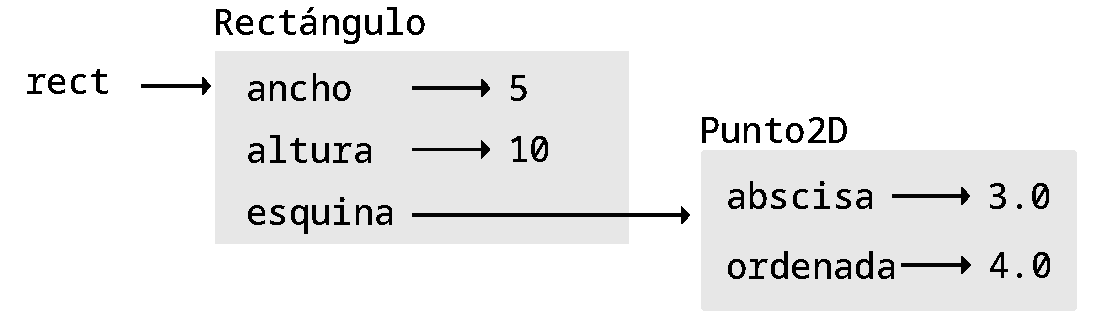
\includegraphics[scale=0.7]{figs/rectangle.pdf}}
\caption{Diagrama de objeto.}
\label{fig.rectangle}
\end{figure}

\index{state diagram}
\index{diagram!state}
\index{object diagram}
\index{diagram!object}
\index{embedded object}
\index{object!embedded}
\index{object!composition}
\index{composition!object}

El uso de un objeto como un atributo de otro objeto, posiblemente
de otra clase, se conoce como {\bf composición de objeto}. 
Un objeto que es un atributo de otro objeto es un objeto 
{\bf embebido}. La composición de objeto hace posible 
definir capas anidadas de abstracción y es una característica
poderosa de la programación orientada a objetos. En nuestro 
ejemplo de ``geometría``, comenzamos a definir un objeto 
a un nivel inferior, una instancia {\tt Punto2D}, y después usamos
ese punto para construir un tipo a un nivel superior, {\tt Rectángulo}.


\section{Instancias como Valores de Retorno}
\index{instance!as return value}
\index{return!value}

Los métodos pueden devolver instancias de otras clase. 
Por ejemplo, la clase {\tt Rectángulo} puede tener métodos
de devuelven instancias de {\tt Punto2D} para las otras
esquinas:

\begin{lstlisting}
    method punto-superior-der {
        return Punto2D.new(
            abscisa  => $!esquina.abscisa + $!ancho, 
            ordenada => $!esquina.ordenada + $!altura
        );
    }
   # otros métodos para las otras esquinas
\end{lstlisting}

Nota que no tenemos que molestarnos en darle un nombre al
punto superior derecho (aunque podríamos si quisiéramos);
podemos crearlo con el constructor y devolverlo inmediatamente.

Podemos usar el nuevo método como sigue:

\begin{lstlisting}
my $puntoSupDer = $rect.punto-superior-der;
say "Esquina superior derecha: ", $puntoSupDer;
# -> Esquina superior derecha: Punto2D.new(abscisa => 9, ordenada => 13)
\end{lstlisting}

\index{type}
Aunque esto no es muy útil en casos simples como este, 
podríamos asegurarnos y declarar un tipo {\tt Punto2D}
para \verb|$puntoSupDer|:

\begin{lstlisting}
my Punto2D $puntoSupDer = $rect.punto-superior-der;
\end{lstlisting} 

De este modo, el código levantará un error si {\tt punto-superior-der}
devuelve algo más que una instancia {\tt Punto2D}.

Similarmente, el método \verb|encontrar-centro| invocado 
sobre un {\tt Rectángulo} devuelve una instancia de 
{\tt Punto2D} que representa el centro del {\tt Rectángulo}:

\begin{lstlisting}
    method encontrar-centro { Punto2D.new(
            abscisa  => $!esquina.abscisa  + $!ancho / 2, 
            ordenada => $!esquina.ordenada + $!altura / 2
        );
    }
\end{lstlisting}
%
Este nuevo método puede ser usado en la siguiente manera:

\begin{lstlisting}
say "Centro = ", $rect.encontrar-centro;
# -> Centro = Punto2D.new(abscisa => 6.5, ordenada => 8.0)
\end{lstlisting}
%

\section{Herencia}
\index{inheritance}
\index{inheritance!class}
\index{class!inheritance}

La herencia es probablemente la característica más 
emblemática de la programación orientada a objetos.
Es un mecanismo a través del cual es posible derivar una
clase de otra clase. La herencia es una de las maneras 
estándares de implementar la reutilización de código en la
programación orientada a objeto. Es también otra manera útil 
de definir capas sucesivas de abstracción y una 
jerarquía de tipos.

\subsection{La Clase Pixel}
\index{class!Pixel}
\index{Pixel class}

La clase {\tt Punto2D} es muy general y podría usarse para
una variedad de propósitos: geometría, gráficas vectoriales, 
mangas animados, etc. Podríamos querer usarlo para mostrar 
datos gráficos en la pantalla. Para este escenario, crearemos
una nueva clase derivada {\tt Pixel}, agregaremos nuevas 
propiedades al punto, tales como color, quizás transparencia, etc.

?`Necesitamos redefinir todos los atributos y los métodos para la 
nueva clase? No, no necesitamos hacer esto. Podemos definir una 
nueva clase que \emph{hereda} las propiedades de la clase base 
{\tt Punto2D} y solo modificamos lo que no es adecuado o agregamos nuevas
características si las necesitamos. Aquí, queremos un nuevo
atributo para representar el color de un píxel y probablemente
algunos otros métodos para manejar este nuevo atributo.

De acuerdo a los estándares más comunes, un color es definido
por tres enteros (realmente tres octetos, i.e., enteros entre 
0 y 255 en la notación decimal), que representan los componentes
rojo, verde y azul de un píxel. Esta combinación de componentes es normalmente
conocida como RGB (sigla en inglés de {\bf R}ed, {\bf G}reen y {\bf B}lue en inglés):
\index{class!child}
\index{Pixel class}
\index{RGB}
\index{octet}

\begin{lstlisting}
class Pixel is Punto2D {
    has %.color is rw;

    method cambiar_color(%tono) {
        %!color = %tono
    }
    method cambiar_color2(Int $rojo, Int $verde, Int $azul) {
        # signatura usando parámetros de posición
        %!color = (rojo => $rojo, verde => $verde, azul => $azul)
    }
}
\end{lstlisting}

\index{parameter!positional}
\index{parameter!named}
\index{positional parameter}
\index{octet}
\index{is!subclassing trait}
La nueva clase \emph{hereda} las propiedades de la {\tt Punto2D}
gracias al rasgo {\tt is Punto2D}, excepto posiblemente
aquellos que son explícitamente modificados (o anulados) o agregados
en la nueva clase. Esta nueva clase es algunas veces llamada
una clase hija o subclase, mientras que {\tt Punto2D} es la
clase padre, clase base o superclase. La creación de esta nueva
clase basada en {\tt Punto2D} se como {\bf subclassing} de la 
clase base {\tt Punto2D}.
\index{class!parent}
\index{class!child}
\index{class!subclass}
\index{subclassing}
\index{overriding a method}
\index{method!overriding}

La nueva clase hija hereda los atributos {\tt abscisa} y 
{\tt ordenada} de la clase padre {\tt Punto2D} (y sus 
propiedades específicas si tienen algunas), al igual que los
métodos tales como {\tt coordenadas} el cual es definido en
la clase padre. La clase hija tiene un nuevo atributo (el color)
y dos métodos nuevos.

Instanciar un objeto {\tt Pixel} es tan fácil como antes,
solo necesitamos agregar un argumento adicional correspondiente
al nuevo atributo cuando invoquemos el constructor {\tt new}:
\begin{lstlisting}
my $pix = Pixel.new(
	:abscisa(3.3),
	:ordenada(4.2),
	color => {rojo => 34, verde => 233, azul => 145}, 
);

say "El píxel original tiene los siguientes colores:", $pix.color;
\end{lstlisting}

In the {\tt Pixel} class definition, we have written 
two different methods for changing the color 
only to illustrate two possible syntax formats, for pedagogical 
purposes.

En la definición de la clase {\tt Pixel}, escribimos dos métodos
diferentes para cambiar el color solo para ilustrar posibles 
formatos de sintaxis, para propósitos pedagógicos. El primer método
recibe un hash como un parámetro, y el segundo usa parámetros de posición,
los cuales forzan al usuario recordar el orden (RGB) en el cual los
argumentos deben pasarse; esto puede ser una fuente de errores y 
debería evitarse cuando el número de parámetros excede un cierto 
límite (lo cual se dejará al lector). Por otro lado, cualquier 
persona que trabaja con gráficas sabe de memoria la convención estándar 
del orden de los colores (i.e., RGB). También, el segundo método
tiene la ventaja de habilitar el chequeo de tipo (los argumentos
deben ser números enteros). Esto es un ejemplo simplificado; en la
vida real, sería deseable chequear si los parámetros son octetos, i.e.,
enteros entre 0 y 255 (lo cual se podría hacer al añadir un
una restricción de tipo o al definir un subconjunto del tipo entero).
\index{subset}
\index{RGB}
\index{octet}

Usar la nueva clase {\tt Pixel} es bien directo:

\begin{lstlisting}
say "Colores originales: ", $pix.color;

$pix.cambiar_color({:rojo(195), :verde(110), :azul(70),});
say "Colores modificados: ", $pix.color;
say "Nuevas características del píxel:";
printf "\tAbscisa: %.2f\n\tOrdenada: %.2f\n\tColores: R: %d, G: %d, B: %d\n",
       $pix.abscisa, $pix.ordenada, 
       $pix.color<rojo>, $pix.color{"verde"}, $pix.color{"azul"};

$pix.cambiar_color2(90, 180, 30);  # argumentos de posición
say "Nuevos colores:  
\tR: {$pix.color<rojo>}, G: {$pix.color<verde>}, B: {$pix.color<azul>} ";
\end{lstlisting}

Esto muestra lo siguiente en la pantalla:

\begin{lstlisting}
Colores originales: {azul => 145, rojo => 34, verde => 233}
Colores modificados: {azul => 70, rojo => 195, verde => 110}
Nuevas características del píxel:
Abscisa: 3.30
Ordenada: 4.20
Colores: R: 195, G: 110, B: 70
Nuevos colores:  
R: 90, G: 180, B: 30 
\end{lstlisting}

Para decir la verdad, no era necesario usar dos métodos con
nombres diferentes, \verb|cambiar_color| y \verb|cambiar_color2|,
como hicimos en la definición de la clase {\tt Pixel} para 
simplificar el asunto. Funcionaría de la misma manera si usáramos
estas definiciones:
\index{Pixel class}
\index{method dispatch}

\begin{lstlisting}
    multi method cambiar_color(%tono) {
        self.color = %tono
    }
    multi method cambiar_color(Int $rojo, Int $verde, Int $azul) {
        # signatura usando parámetros de posición
        self.color = (rojo => $rojo, verde => $verde, azul => $azul)
    }
\end{lstlisting} 

Debido a que el método multi se define dos veces, con el 
mismo nombre pero diferente signatura, el sistema de objeto
es capaz de despachar la invocación al método correcto.
\index{method!dispatch}
\index{multi method}


\subsection{La Clase PuntoMovible}
\index{class!MovablePoint}
\index{MovablePoint class}

Los atributos \verb|$.abscisa| y \verb|$.ordenada| de la 
clase {\tt Punto2D} son por defecto atributos con solo
acceso de lectura. Después de todo, cuando defines un punto
en el plano, usualmente tiene una posición fija y generalmente 
no hay razón para cambiar su coordenada.

Sin embargo, supón que nuestra aplicación es acerca de la
cinemática (la rama de la física que estudia el movimiento
de puntos o cuerpos) o es un videojuego. En tal caso, probablemente
queremos que nuestros puntos (o conjunto de puntos) puedan 
moverse. Necesitamos una nueva clase, {\tt PuntoMovible},
para habilitar la modificación de las coordenadas.

No necesitamos redefinir todos los atributos y métodos para
la nueva clase. Otra vez, podemos definir una nueva clase
que \emph{herede} las propiedades de la clase base {\tt Punto2D}
y solo modifique aquello que no es adecuado o agregue 
nuevas características que necesitemos, por ejemplo:

\begin{lstlisting}
class PuntoMovible is Punto2D {
    has Numeric $.abscisa is rw;
    has Numeric $.ordenada is rw;
    
    method mover (Numeric $x, Numeric $y) {
        $.abscisa  += $x;
        $.ordenada += $y;
    }
}
\end{lstlisting}

\index{is!subclassing trait}
La nueva clase hereda las propiedades de {\tt Punto2D} 
gracias al rasgo {\tt is Punto2D}, excepto que aquellos
que son explícitamente modificados (o anulados) o agregados
en la nueva clase. Los métodos que existen en la clase padre
y se redefinen en la clase hija se dice que son \emph{anulados}
dentro esa clase.
\index{class!parent}
\index{class!child}
\index{class!subclass}
\index{subclassing}
\index{overriding a method}
\index{method!overriding}

Aquí, los atributos \verb|$.abscisa| y \verb|$.ordenada| 
se redefinen con acceso de lectura y escritura (a través del rasgo
{\tt is rw}) y un método nuevo, {\tt mover}, es definido para modificar
la posición de un punto al añadir los parámetros recibidos a las
coordenadas del punto.
\index{is rw trait}

Nota que hemos usado parámetros de posición para el método {\tt mover}. 
Dijimos que es usualmente mejor por motivos de claridad usar parámetros
nombrados, pero hemos usado solo dos parámetros aquí; debido a que 
es bastante simple recordar que el parámetro \verb|$x| debería venir
antes que el parámetro \verb|$y|. Esto fue una ocasión para ilustrar la
posibilidad de usar parámetros de posición.
\index{positional parameter}
\index{parameter!positional}
\index{parameter!named}
\index{named parameter}

Ahora podemos probar nuestra clase hija, crear una instancia 
{\tt PuntoMovible}, mostrar sus características, moverla a una
posición diferente, y mostrar la posición nueva. 

\begin{lstlisting}
my $punto = PuntoMovible.new(
    abscisa => 6,
    ordenada => 7,
    );

say "Coordenadas: ", $punto.coordenadas;
say "Distancia al origen: ", $punto.distancia-al-centro.round(0.01);
printf "%s: radio = %.4f, theta (rad) = %.4f\n", 
    "Coordenadas polares", $punto.coordenadas-polares;

say "--> Moviendo el punto.";
$punto.mover(4, 5);
say "Nuevas coordenadas: ", $punto.coordenadas;
say "Distancia al origen: ", $punto.distancia-al-centro.round(0.01);
printf "%s: radio = %.4f, theta (rad) = %.4f\n", 
    "Coordenadas polares", $punto.coordenadas-polares;
\end{lstlisting}

Esto produce la siguiente salida:

\begin{lstlisting}
Coordenadas: (6 7)
Distancia al origen: 9.22
Coordenadas polares: radio = 9.2195, theta (rad) = 0.8622
--> Moviendo el punto.
Nuevas Coordenadas: (10 12)
Distancia al origen: 15.62
Coordenadas polares: radio = 15.6205, theta (rad) = 0.8761
\end{lstlisting}

\index{polar coordinates}
\index{coordinates!polar}
Aquí, cuando el usuario invoca los métodos {\tt coordenadas},
{\tt distancia-al-centro}, y {\tt coordenadas-polares}, Perl
encuentra que dichos métodos no existen en la clase {\tt PuntoMovible}.
Pero, dado que \verb|PuntoMovible| es una subclase de {\tt Punto2D},
el programa hace una búsqueda de estos nombres en la clase padre, 
y los invoca si los encuentra. Si no los encuentra, entonces podría
buscar en el padre de la clase padre para ver si se encuentran ahí, etc.


\subsection{Herencia Múltiple: Atractiva Pero, es de Sabio Utilizarla?}

En la programación orientada a objeto, el mecanismo de herencia
es una manera tradicional de reutilizar código. Es probablemente 
la forma más común de hacerlo.

Un clase puede tener varias clases padres y, por lo tanto,
ser una subclase de otras clases. Esto es lo que se conoce como
{\bf herencia múltiple}. Podríamos construir una nueva 
clase {\tt PixelMovible} la cual hereda de {\tt PuntoMovible} 
y de {\tt Pixel} (e, indirectamente, de {\tt Punto2D}). Técnicamente,
puedes hacer esto fácilmente en Perl:

\begin{lstlisting}
class PixelMovible is PuntoMovible is Pixel {
    # ...
}
\end{lstlisting}

Ahora, {\tt PixelMovible} es una clase de {\tt PuntoMovible}
y {\tt Pixel} y hereda de ambas clases padres.
\index{subclass}
\index{class!parent}

Esto luce bastante prometedor, pero sucede que tiende a ser
más complicado de lo esperado en situaciones reales. Si existe
un conflicto (por ejemplo una colisión de nombre entre dos método),
cuál debe prevalecer? Algunos mecanismo existen para manejar tales
situaciones (por ejemplo en el lenguaje de programación C++), y
Perl tiene métodos metaobjetos para encontrar información
sobre el orden de resolución de los métodos (MRO por sus siglas en inglés),
pero esto puede rápidamente conducir a varios problemas de diseño y a
errores (\emph{bugs}) que son sutiles y complicados. En resumen, 
mientra la herencia múltiple originalmente lucía como una atractiva idea, 
resultó ser en algo muy complicado de dominar,
porque crea dependencias múltiples, y usualmente implícitas, que son 
difíciles de arreglar.

Esta es la razón por la cual, contrario a C++, relativamente reciente lenguajes de programación orientados a objetos como Java (el cual surgió no tan recientemente, en 1995) han decidido no implementar herencia múltiple.

Perl~6 no quiere prohibir tales cosas y como resultado te permite
hacer uso de la herencia múltiple si deseas, la cual puede ser 
muy útil para casos simples. Así que no la descarte innecesariamente,
pero recuerdas que, contrario a las expectaciones originales, 
la herencia múltiple usualmente conduce a un desastre y resulta
ser incontrolable.

Perl ofrece mejores conceptos para encargarse de tales situaciones, como
veremos en un momento.

\section{Roles y Composición}
\index{role}
\index{inheritance}

La herencia es un concepto poderoso para describir un árbol jerárquico de
conceptos. Por ejemplo, puedes pensar de una jerarquía de figuras geométricas
que tienen una o más propiedades específicas: 
\begin{enumerate}
\item Polígono

\index{quadrilateral}
\item Cuadrilátero (un polígono con cuatro lados y cuatro esquinas)

\index{trapezoid}
\item Trapezoide (un cuadrilátero con un par de lados paralelos)

\index{parallelogram}
\item Paralelogramo (un trapezoide con dos pares de lados paralelos y lados
opuestos de la misma longitud)

\index{rectangle}
\item Rectángulo (un paralelogramo con cuatro ángulos rectos)

\index{square}
\item Cuadrado (un rectángulo con cuatro lados iguales)
\end{enumerate}

\index{rhombus}
Es relativamente fácil de imaginar una serie de clases con un árbol de
herencia jerárquica que refleje esas propiedades. Se vuelve más 
complicado, sin embargo, si agregamos el rombo (un paralelogramo con
todos los lados iguales), porque el cuadrado es ahora \emph{también}
un rombo con cuatro ángulos rectos. La clase cuadrado sería una 
subclase del rectángulo y del rombo, y podríamos tener un posible
caso de herencia múltiple.

\index{integer} \index{rational} \index{real number} \index{complex number}
\index{vertebrate} \index{mammal} \index{carnivoran}
\index{canid} \index{dog}
Similarmente, podemos pensar acerca de un árbol de clases con herencia
anidada que representan varios tipos de números (e.g., entero, 
racional, real, complejo) o especies de animales (e.g., vertebrado, 
mamífero, carnívoro, canino, perro, setter irlandés).

\index{hierarchical model}
Estos son ejemplos grandiosos de herencia, pero el mundo real es
raramente jerárquico, y es usualmente difícil de forzar cada caso 
a encajar en un modelo jerárquico.

\index{role}
Esta es una de la razones por la cual Perl introduce la noción
de roles. Un rol es un conjunto de comportamientos o acciones
que pueden compartirse entre varias clases. Técnicamente, un rol
es una colección de métodos (posiblemente con algunos atributos);
es por lo tanto similar a una clase, pero la primera diferencia
obvia es que un rol no está diseñado para ser instanciado como
un objeto (aunque los roles pueden ser promovidos al estado de
clases). La segunda diferencia, quizás la más importante, es que los
roles no heredan: ellos se usan al ser aplicados a una clase 
o/y una composición.

\subsection{Clases y Roles: Un Ejemplo}

\index{vertebrate} \index{mammal} \index{dog}
Volvamos con los vertebrados, mamíferos y perros. Un perro
es un mamífero y hereda algunas características de los 
mamíferos tales como una neocórtex (una región del cerebro),
pelo, y glándulas mamarias, también como una columna vertebral,
la cual todos los mamíferos (incluyendo los peces, aves, reptiles, etc.)
heredan de los vertebrados. Hasta ahora, la jerarquía de la clase
parece simple y natural.

\index{feral animal}
\index{pet animal}
No obstante los perros pueden tener diferentes características y
comportamientos. Para citar un artículo de Wikipedia sobre los perros:
``Los perros tienen un sin número de \emph{roles} para las personas
entre los que figuran la caza, el pastoreo, halar cargas pesadas, asistir
a la policía y el ejército, compañía y, recientemente, asistir a
individuos incapacitados`` (énfasis añadido). Los perros también pueden 
ser animales salvajes (i.e, animales que viven en ambientes silvestres
pero que han descendido de individuos domesticados) o perros callejeros.
Todos comportamientos adicionales pueden añadirse a la clase perro.
Similarmente, un gato, otro mamífero, puede ser una mascota o
un animal salvaje. Los mustangos, caballos salvajes de Norteámerica,
también son animales salvajes, descendientes en algún tiempo de caballos
domesticados; pero un mustango puede capturarse y puesto devuelta
en un estado domesticado. Este retorno a lo salvaje de animales
silvestres no está limitado a los mamíferos: las palomas que viven
en nuestras ciudades descendieron una vez de palomas mensajeras
usadas en el pasado. Puede hasta ocurrir con invertebrados, tales
como enjambres de abejas melíferas.

Es aparente que un modelo jerárquico de arboles de herencia
no está adaptado para describir tales comportamientos.

\index{vertebrate} \index{mammal} \index{dog}
Podemos definir clases para los perros, los gatos, y los 
caballos como subclases de mamíferos (los cuales también heredan
de los vertebrados). Además de eso, podemos definir roles para mascotas
o animales salvajes. En adición, podemos crear nuevas clases
que son subclases de las clases perro, gato y caballo y que 
tienen algunos roles específicos. Del mismo modo, podemos
asignar roles a instancias individuales de una clase. Esto
podría lucir así (este un ejemplo ficticio que no se puede probar):

\begin{lstlisting}
class Vertebrado { method hablar {say "vertebrado"};}
class Mamífero is Vertebrado  { method hablar { say "mamífero" } }
class Ave      is Vertebrado  { method volar     {} }
class Perro    is Mamífero    { method ladrar    {} }
class Caballo  is Mamífero    { method relinchar {} }
class Gato     is Mamífero    { method maullar   {} }
class Ratón    is Mamífero    { method chillar   {} }
class Pato     is Ave         { method graznar   {} }
# ...

role Animal-mascota { 
    method es-compañero() {...} 
    # otros métodos
}
role Ovejero     { ... }    # pastor de ovejas
role Salvaje     { ... }    # animal en un ambiente salvaje
role Guía        { ... }    # guía de los ciegos
role Humano-comp { ... }    # animal que se comporta como un humano
# ...

class Perro-guía          is Perro   does Guía           { ... }
class Perro-ovejero       is Perro   does Ovejero        { ... }
class Perro-callejero     is Perro   does Salvaje        { ... }
class Gato-mascota        is Gato    does Animal-mascota { ... }
class Gato-salvaje        is Gato    does Salvaje        { ... }
class Mustago             is Caballo does Salvaje        { ... }
class Canario-dom         is Ave 	 does Animal-mascota { ... }
# ...
# Un rol se puede aplicar a instancias:
my $garfield = Gato-mascota.new(...);
my $mickey   = Ratón.new(...);
$mickey does Humano-comp;
my $donald   = Pato.new(...);
$donald does Humano-comp; 
my $pluto    = Perro.new(...);
$pluto does Animal-mascota;
my $snoopy   = Perro.new(...);
$snoopy does Animal-mascota does Humano-comp;
\end{lstlisting}
 
\index{role!application}
\index{does trait}
\index{trait!does}
\index{trait!is}
Un rol se aplica a una clase o a un objeto con el rasgo
{\tt does} (opuesto a {\tt is} para la herencia). Estas dos
palabras claves diferentes reflejan la diferencia semántica
asociada con ellas: componer un rol en una clase u objeto
provee dicha clase u objeto con el \emph{comportamiento suplementario}
asociado con el rol, pero esto no significa que al objeto
recibir el rol es la \emph{misma cosa} o de la misma naturaleza como 
el rol.

\index{feral animal}
\index{pet animal}
Si los roles {\tt Animal-mascota} y {\tt Salvaje} hubiesen sido 
definidos como clase, entonces las clases {\tt Gato-mascota} y
{\tt Gato-salvaje} hubiesen experimentado herencia doble,
con los problemas potenciales asociados con eso. Al aplicar
un rol a una clase, evitas construir un árbol de herencia múltiple
que probablemente no se puede justificar y que puede ser difícil de
conceptualizar y manejar. Un uso juicioso de clases y roles puede 
conducir a un modelo que es más simple, más natural, y más cercano
a las relaciones reales entre las entidades y comportamientos 
bajo escrutinio.

\index{multiple inheritance}
\index{method!dispatch}
\index{role!composition}

In adición, si compones varios roles inadvertidamente con dos
métodos que poseen el mismo nombre, esto inmediatamente levanta
un error (a menos que un método con el mismo nombre exista dentro
de la clase y en tal caso, prevalece), en lugar de despachar silenciosamente
a una de los métodos como en el caso de herencia múltiple. En 
ese caso, los conflictos de nombre son identificados inmediatamente
(al tiempo de compilación), lo cual tiene el beneficio de 
encontrar un error inmediatamente, el cual podría no ser
perceptible por un largo tiempo.

\subsection{Composición de un Rol y Reutilización de Código}

Las clases son para manejar instancias y los roles son para
manejar comportamientos y reutilización de código. El siguiente
ejemplo muestra cómo las clases y los roles funcionan bien juntos.
\index{class}
\index{role}
\index{code reuse}

\begin{lstlisting}
role Dibujable {
    has $.color is rw;
    method dibujar { ... }
}
class Figura {
    method area { ... }
}
class Rectángulo is Figura does Dibujable {
    has $.ancho;
    has $.altura;
    method area {
        $!ancho * $!ancho;
    }
    method dibujar() {
        for 1..$.altura {
            say 'x' x $.ancho;
        }
    }
}
Rectángulo.new(ancho => 10, altura => 4).dibujar;
\end{lstlisting}

\index{ellipsis}
Ten presente que la intención de los puntos suspensivos
\verb|...| usados en el código anterior es representar
código que se deja para tu implementación. Sin embargo, esto
es actualmente código válido y se compilará y hasta se 
ejecutará sin ningún problema. Los puntos suspensivos 
son usados para representar una funcionalidad que no se ha
implementado todavía pero que se hará en el futuro. Esto funcionará
siempre y cuando to no invoques estos métodos (lo que producirá un 
error de ejecución) o crees una situación donde ellos necesitarían
estar definidos (lo que ocasionará un error de compilación).
En el caso del método {\tt dibujar} en el role {\tt Dibujable},
la composición de rol en la clase {\tt Rectángulo} funciona
solo porque {\tt dibujar} es redefinido en la clase {\tt Rectángulo};
sin esta redefinición, hubiese levantado un error al tiempo de
compilación. Similarmente, el código \verb|method area { ... }|
de la clase {\tt Figura} levantaría un error al tiempo de
ejecución si fuera llamado sin haber sido redefinido en
la clase {\tt Rectángulo}. Los puntos suspensivos se han usado 
aquí como una manera conveniente de representar código cuyo 
implementación no es importante para nuestro ejemplo porque se está
redefiniendo de cualquier modo. En código real, es probablemente
recomendado no usar puntos suspensivos, excepto como expediente temporario
para código que no se ha desarrollado todavía pero que será
implementado.

El código de más arriba dibuja un rectángulo ASCII:
\begin{lstlisting}
~ perl6 test_drawable.pl6
xxxxxxxxxx
xxxxxxxxxx
xxxxxxxxxx
xxxxxxxxxx
\end{lstlisting}

\subsection{Roles, Clases, Objetos, y Tipos}
\index{role}
\index{class}
\index{object}
\index{type}

Un rol se puede aplicar a una clase entera o solamente a 
algunas instancias de la clase:

\begin{lstlisting}
role Guía { ...}
class Perro-guía is Perro does Guía { 
    ... 
}  # Componiendo el rol Guía en la clase Perro-guía
   # la cual hereda de la clase Perro

my $perrito = new Perro; # creando un objeto Perro
$doggy does Guide;       # aplicando el rol al objeto
\end{lstlisting}

\index{type}
\index{role!type}
\index{type!-defining role}
\index{guide}
Los roles y las clases son diferentes, pero ambos son tipos
o definen tipos. Esto significa que un rol puede usarse como
un tipo para una declaración de variable donde esperaría el 
nombre de una clase. Por ejemplo, el rol {\tt Guía} en el fragmento
de código anterior efectivamente crea un tipo {\tt Guía}. Así que
un rol {\tt Invidente} para un humano podría tener un atributo
de tipo {\tt Guía}, el cual representaría un perro-guía, un 
caballo-guía, un humano-guía o hasta un robot-guía.

\begin{lstlisting}
class Humano {
    has Perro $perro;  # Puede contener cualquier perro,
    		  # con o sin un rol guía
}
role Invidente {
    has Guía $guía;  # Puede contener un tipo Guía, 
    	  	# un perro, un caballo, un humano, o un robot
}
\end{lstlisting}

\index{type!built-in}

Una mayoría de los tipos integrados de Perl~6 son definidos
por roles y no clases, tales como {\tt IO}, {\tt Iterable}, 
{\tt Iterator}, {\tt Numeric}, {\tt Rational}, {\tt Real},
etc.

\section{Delegación de Método}
\index{delegation}


La {\bf Delegación} es otra manera de enlazar un objeto a otra pieza 
de código. La técnica de delegación ha sido estudia extensivamente 
al nivel teórico e implementada en algunos cuantos lenguajes 
especializados de investigación, pero la implementación de
delegación en los lenguajes generalistas convencionales
es bien inusual.

En lugar de definir métodos en una clase o en un rol, la idea 
es invocar los métodos perteneciente a otro objeto, como si fueran
métodos de la clase actual. En Perl~6, la delegación puede realizarse
al nivel de una clase o un rol. Un objeto delegado es simplemente
un atributo definido en una clase o en un rol con la palabra clave
{\tt handles} que posibilita especificar cuales métodos del objeto 
delegado pueden ser usados en la clase actual:

\index{Cervantes, Miguel de} \index{Shakespeare, William} 
\index{Chekhov, Anton} \index{Schiller, Friedrich} \index{Hamlet} 
\index{Don-Quijote} \index{Don-Carlos} \index{Three Sisters}
\begin{lstlisting}
class ClaseBase {
    method Don-Quijote()    { "Cervantes"   }
    method Hamlet()         { "Shakespeare" }
    method Three-Sisters () { "Chekhov"     }
    method Don-Carlos()     { "Schiller"    }
}

class Uses { 
    has $.base is rw handles < Don-Quijote Hamlet Three-Sisters >;
}

my $user = Uses.new;
$user.base = ClaseBase.new(); # implementando un object-handler
say $user.Don-Quijote;
say $user.Hamlet;
say $user.Three-Sisters;
say $user.Don-Carlos;
\end{lstlisting}

Esto muestra lo siguiente:

\begin{lstlisting}
Cervantes
Shakespeare
Chekhov
Method 'Don-Carlos' not found for invocant of class 'Uses'
  in block <unit> at delegate.pl6 line 16
\end{lstlisting}
\index{invocant}

El programa muestra apropiadamente los nombres de los
escritores que los primeros tres métodos devuelve, porque ellos
han sido más o menos ``importados`` en la clase {\tt Uses}, pero 
falla con el último, porque ``Don-Carlos`` no es parte de la 
lista del handler. El error en el último método es una excepción al
tiempo de ejecución y el programa terminaría la ejecución ahí aún
hubiera algún código correcto después. 

Nota que la clase {\tt Uses} no sabe de donde los métodos 
serán importados; solo sabe sobre los nombres de los 
métodos que serán importados. Solamente cuando el objeto
\verb|$user| es creado y el atributo \verb|$user.base|
es añadido, el objeto es dinámicamente con los métodos
definidos en {\tt ClaseBase}. Casualmente, este proceso
puede hacerse en un solo paso:

\begin{lstlisting}
my $user = Uses.new( base => ClaseBase.new() );
\end{lstlisting}

No hay necesidad de enumerar los métodos que serán manipulados.
La clase {\tt Uses} puede importar todos los métodos de 
{\tt ClaseBase}:

\begin{lstlisting}
class Uses { 
    has $.base is rw handles ClaseBase;
}
\end{lstlisting}

Esto funcionará como antes, excepto que no fallará con el método
{\tt Don-Carlos} ahora, debido a que este método fue importado también:

\begin{lstlisting}
Cervantes
Shakespeare
Chekhov
Schiller
\end{lstlisting} 

\section{Polimorfismo}
\index{polymorphism}
\index{interface}

El polimorfismo es una manera de suplir un interfaz común o 
relacionada a tipos diferentes. En cierta manera, los ejemplos
de herencia que estudiamos anteriormente ofrecen una forma
de polimorfismo: los métodos {\tt coordenadas}, {\tt distancia-al-centro}, y {\tt coordenadas-polares} son polimórficos, debido a que ellos pueden aplicar a los tipos
{\tt Punto2D}, {\tt PuntoMovible} y {\tt Pixel}. Hablaremos de
polimorfismo cuando los métodos relevantes o funciones hacen cada uno algo diferente, por lo menos al nivel de implementación, aún
compartan el mismo nombre y misma interfaz.

\index{multi!subroutine}
\index{invocant}
Fuera de la programación orientada a objeto (POO), las subrutinas
\emph{multi} de Perl implementan una forma de polimorfismo,
dado que se comportan de forma diferente dependiendo del tipo
y número de sus argumentos. Dentro del contexto POO, es
usualmente el tipo del invocante (su clase o posiblemente uno de
sus roles) que determinará, usualmente al tiempo de 
ejecución, cuales de los posibles métodos será invocado.

Por ejemplo, podríamos querer crear una nueva clase para 
puntos en el espacio tridimensional. Los métodos tendrán 
que ser diferentes, pero sería interesante ofrecer al usuario
un interfaz que es igual (o casi igual)  a aquella de los
puntos en dos dimensiones:
\index{Point3D class}

\begin{lstlisting}
class Punto3D {
    has Numeric $.x;
    has Numeric $.y;
    has Numeric $.z;
    
    method coordenadas () {      # método de acceso a las 3 coordenadas
    	return $.x, $.y, $.z
    }
    method distancia-al-centro () {
        return ($.x ** 2 + $.y ** 2 + $.z ** 2) ** 0.5
    }
    method coordenadas-polares () {
    	return self.coordenadas-esféricas;
    }
    method coordenadas-esféricas {
    	my $rho = $.distance2center;
    	my $longitud = atan2 $.y, $.x;          # theta
    	my $latitud = acos $.z / $rho;          # phi 
    	return $rho, $longitud, $latitud;
    }
    method coordenadas-cilíndricas {
    	# ...
    }
}
\end{lstlisting}

Los métodos en esta nueva clase no son los mismos que 
en {\tt Punto2D}, pero los métodos con semánticas similares
tienen el mismo nombre; así que es posible usar cualquiera
de las clases sin perderse con nombres diferentes.

El método {\tt distancia-al-centro} tiene exactamente la misma interfaz. El método {\tt coordenadas} devuelve una lista de tres 
valores en lugar de dos, pero la convención de llamada es la misma. Nota que podría haber sido posible diseñar {\tt Punto2D}
de tal manera que este método devolviera un tercer valor cero, 
para tener exactamente la misma interfaz (después de todo, un punto en el plano podría ser considerado como un punto en el 
espacio 3D con altura cero); cumplir exactamente con la misma
interfaz no es mandatorio, pero solo una posible implementación
que podría hacer una interfaz más intuitiva.
 

\index{polar coordinates}
\index{spherical coordinates}
\index{coordinates!polar}
\index{coordinates!spherical}
La noción de coordenadas polares no tiene un significado 
bien definido en el espacio 3D, pero he elegido mantener el nombre
en nuestra interfaz porque es intuitivamente similar a la idea
de coordenadas esféricas; no hace nada más que invocar 
el método \verb|coordenadas-esféricas| sobre su invocante y
devolver los valores de retorno.
\index{invocant}

Por favor nota que los matemáticos, físicos, astrónomos, ingenieros, geógrafos, y navegadores todos usan el mismo sistema
básico para las coordenadas esféricas, pero sus convenciones
son diferentes con respecto al origen, rango del ángulo, 
unidades medidas de ángulos y dirección de rotación, y el nombre de los varios valores o símbolos asociados con los mismos. 
Así que podrías encontrar diferentes fórmulas en un libro de
texto. Las convenciones y fórmulas que hemos usado son comúnmente
utilizadas en geografía y algunas ramas de las matemáticas. Una clase real de propósito general tendría que tomar en cuenta toda estas convenciones e implementar las convenciones necesarias.

\section{Encapsulación}

\index{encapsulation}
La encapsulación es la idea de ocultar los datos y código 
de una librería o un módulo del usuario. El concepto no es
específico a la programación orientada a objeto, pero 
es parte fundamental de la misma.

\index{accessor}
\index{mutator}
\index{getter}
\index{setter}
En la programación orientada a objetos, la encapsulación 
consiste de proteger los datos en un objeto de manipulación
directa (y de manera inconsistente) por el usuario, quien 
acceder tales datos a través de los métodos. Esto se logra al
proveer al usuario métodos que son conocidos como \emph{métodos 
de acceso} (o \emph{getters}) y \emph{mutadores} (o \emph{setters}).
Esto hace posible asegurar que las propiedades del objeto 
serán validadas por sus métodos. 


\index{black box}
\index{object!interface}
La encapsulación es una forma poderosa de abstracción
y abstracción procedimental. Visto desde afuera, un
objeto es una caja negra que tiene propiedades y 
comportamientos específicos. De esta forma, estas propiedades
y comportamientos están \emph{ocultos} del usuario. 
No están ocultos en el sentido de que el usuario no puede
saber sobre ellos (por lo menos en el mundo de código 
abierto (\emph{open source}), es fácil saber esto), pero
que están ocultos en el sentido de que es usualmente no posible
usar ese conocimiento para eludir la interfaz proveída.
Esto significa que la implementación interna del objeto 
puede cambiar sin tener que modificar el comportamiento
externo. Si usas conocimiento privilegiado, tu código
probablemente no funcionará correctamente cuando la 
implementación interna sea modificada. Por lo tanto,
no hagas eso.

Varios lenguajes de programación no tienen las mismas reglas para
garantizar encapsulación. Algunos son más estrictos que otros,
algunos son menos estrictos sobre el acceso de lectura que el
acceso de escritura, otros no hacen tal distinción pero más bien
dependen en el nivel de visibilidad especificado por un atributo,
por ejemplo ``public`` o ``private`` (algunas veces con un nivel 
intermedio ``protegido``).

\index{attribute!private}
Perl~6 te permite eligir el modelo de encapsulación que quieres
aplicar a tus objetos y atributos. Todos los atributos son 
privados. Si declaras una clase así:

\begin{lstlisting}
class Punto2D {
    has $!abscisa;
    has $!ordenada;
    # …
    method valor_x { return $!abscisa }
    method valor_y { return $!ordenada }
}
\end{lstlisting}

las coordenadas \verb|$!abscisa| y \verb|$!ordenada|
serán accesible solo dentro de la clase. Esta es la 
razón por la cual hemos añadido métodos de acceso.
Además, los atributos son inmutables por defecto.

Pero como vimos anteriormente, si declaras
esta clase así:

\begin{lstlisting}
class Punto2D {
    has $.abscisa;
    has $.ordenada;
    # ...
}
\end{lstlisting}

las coordenadas serán todavía atributos privados, pero
Perl~6 generará métodos de acceso automáticamente con los
mismos nombres de los atributos. De esta manera, se pueden
acceder fuera de la clase casi como si fueran públicos:
\index{attribute!public}

\begin{lstlisting}
class Punto2D {
    # ...
}
my $punto = Punto2D.new(abscisa => 2, ordenada => 3);
say $punto.abscisa;       # -> 2
\end{lstlisting}

\index{attribute!mutable}
\index{attribute!immutable}
El rasgo {\tt is rw} maneja separadamente si un atributo 
es mutable o no. En resumen, Perl~6 ofrece un modo acceso por
defecto, pero puedes configurarlo y lo que necesitas.


\subsection{Métodos Privados}
\index{private method}
\index{method!private}
\index{interface}

Los métodos son la manera normal de usar objetos, ya sea con
solo acceso de lectura o con acceso de lectura y escritura. 
Usualmente forman la \emph{interfaz} de una clase, que es la
parte de la clase que es pública y disponible para los programadores que deseen usarla. Es por lo tanto natural y legítimo que los métodos sean públicos, i.e, accesibles fuera
de la clase.
\index{method!public}
\index{public method}

Pero una clase puede también contener numerosos métodos
que son parte de la receta de cocina interna de la clase, i.e.,
la forma en la que hace las cosas internamente, y que no están
destinadas a ser usadas fuera de la clase. Es posible prevenir 
su uso fuera de la clase al hacer estos métodos privados. 
Un método privado de Perl~6 se prefija con un signo de 
exclamación:

\begin{lstlisting}
method !comportamiento-privado($x, $y) {
    ...
}
\end{lstlisting}

También necesitarás usar un signo de exclamación para llamarlos:

\begin{lstlisting}
$mi-objecto!comportamiento-privado($val1, $val2)
\end{lstlisting}

\index{private method}
\index{method!private}
Los métodos privados son realmente internos de una clase 
dada. En particular, ellos no son heredados por las clases hijas.


\subsection{Construir Objetos con Atributos Privados}

Construir objetos con atributos privados trae consigo una
pequeña dificultad. Consideremos el siguiente programa:
\index{private attribute}

\begin{lstlisting}
class Punto3D {
    has $.x;
    has $.y;
    has $!z;
    
    method coord_valores {
        return ($!x, $!y, $!z);
    }
};

my $a = Punto3D.new(x => 23, y => 42, z => 2);
say $_ for $a.coord_valores;
\end{lstlisting}

\index{attribute!private}
\index{attribute!public}
En este ejemplo, hemos declarado a \verb|$.x| y \verb|$.y|
como atributos ``públicos`` (por así decirlo), y a \verb|$!z|
como un atributo verdaderamente privado. La ejecución de 
este código muestra lo siguiente:

\begin{lstlisting}
23
42
(Any)
\end{lstlisting}

?`Qué está sucediendo? Parece que el método \verb|coord_valores|
es incapaz de leer el contenido de \verb|$!z|, dado que 
devuelve un valor indefinido. Este método es definido dentro
de la clase y debería ser capaz de acceder este atributo. De hecho,
\verb|coord_valores| no es el problema, sino que \verb|$!z| no está
definido dentro del objeto, porque no se inicializó apropiadamente
durante la creación del objeto.
\index{new!constructor}
\index{constructor!new}
La culpa yace con el constructor implícito {\tt new} que, por
defecto, inicializa solo los atributos ``públicos``.

\index{submethod}
Aquí la solución más simple es probablemente añadir el 
submétodo {\tt BUILD}  en la definición de la clase.
\index{BUILD submethod}

\index{submethod}
\index{subclass}
\index{type}
Un {\tt submétodo} es un método público de una clase que 
no es heredado por sus clases hijas. Semánticamente, es realmente
equivalente a una subrutina, pero se invoca con una sintaxis 
de método (de ahí su nombre). Los submétodos son especialmente útiles
al realizar las tareas de construir y destruir un objeto que no 
deberían ser heredadas por las subclases, también como para las
tareas que son tan específicas para tipo particular que las clases
derivadas tendrán que seguramente modificarlas.

Inicializar los atributos privados durante la instanciación de un objeto
podría lucir así:

\begin{lstlisting}
class Punto3D {
    has $.x;
    has $.y;
    has $!z;

    submethod BUILD (:$!x, :$!y, :$!z) {
        say "!`Inicialización!";
        $!x := $!x; 
        $!y := $!y; 
        $!z := $!z;
    }
    method coord_valores {
        return ($!x, $!y, $!z);
    }
};

my $a = Punto3D.new(x => 23, y => 42, z => 2);
say $_ for $a.coord_valores;
\end{lstlisting}

El programa ahora funciona como se deseaba y muestra 
todos los atributos:

\begin{lstlisting}
!`Inicialización!
23
42
2
\end{lstlisting}

Esto funciona porque el constructor por defecto {\tt new},
un método definido la superclase suprema {\tt Mu} y heredado
por cualquier clase de Perl~6, llama al submétodo por defecto
{\tt BUILD}. Si redefinimos a {\tt BUILD} en nuestra clase, entonces
reemplazará el submétodo por defecto que {\tt new} llama. Al redefinir
a {\tt BUILD}, forzamos el constructor a tomar en cuenta el
atributo privado que no se usó previamente.

Un poco de simplificación es posible. Dado que los argumentos
que se pasan a una rutina enlazan los argumentos a los parámetros,
un paso de enlace separado es innecesario si los atributos se usan
como parámetros. Por lo tanto, el submétodo {\tt BUILD} en el ejemplo
anterior podría también escribirse tan simple como esto:
\index{BUILD submethod}

\begin{lstlisting}
    submethod BUILD(:$!x, :$!y, :$!z) {
        say "!`Inicialización!";
    }
\end{lstlisting}

\index{overriding a method}
\index{named parameter}
\index{positional parameter}
\index{parameter!named}
\index{parameter!positional}
\index{constructor!new}
\index{new!constructor}

Mientras hablamos de las particularidades de la construcción de un objeto,
nota que debido a que {\tt new} es un método heredado desde la superclase
{\tt Mu}, puedes anularlo si lo prefieres. El constructor por defecto
{\tt new} puede usarse solo con argumentos nombrados. Asumiendo que realmente
quieras parámetros de posición, puedes anular a {\tt new} con tu 
propio método, de esta manera:
\index{new!constructor} 
\index{constructor!new}

\begin{lstlisting}
class Punto2D {
    has Numeric $.abscisa;
    has Numeric $.ordenada;

    method new ($x, $y) {
        self.bless(abscisa => $x, ordenada => $y);
    }
    method coordenadas {        # método de acceso a las coordenadas
        return (self.abscisa, self.ordenada)
    }
    # otros métodos
};

my $punto = Punto2D.new(3, 5);
say $_ for $punto.coordenadas;
\end{lstlisting}

Esto mostrará las dos coordenadas. {\tt bless} es un método
de nivel inferior para la construcción de objetos, heredado
desde {\tt Mu} y llamado automáticamente cuando invocas a {\tt new}
para construir un objeto. Usualmente no necesitas saber sobre 
ese método, excepto cuando quieres escribir tu propio
constructor personalizado.

\index{constructor!custom}
Puedes darle un nombre diferente al constructor, por ejemplo:

\begin{lstlisting}
class Punto2D {
    has Numeric $.abscisa;
    has Numeric $.ordenada;

    method construir ($x, $y) {
        self.bless(abscisa => $x, ordenada => $y);
    }
    method coordenadas {        # método de acceso a las coordenadas
        return (self.abscisa, self.ordenada)
    }
    # otros métodos
};

my $punto = Punto2D.construir(3, 5);
say $_ for $punto.coordenadas;
\end{lstlisting}

Aunque deberías pensar dos veces antes de anular a {\tt new} 
o crear tu propio constructor personalizado con un nombre diferente,
dado que podría hacer más difícil la creación de subclases de la 
clase {\tt Punto2D}.



\section{Interfaz e Implementación}

Una de las metas del diseño orientado a objetos es crear software
más fácil de mantener, lo que significa que mantener el programa
funcionando cuando otras partes del sistema cambia, y modificar el 
programa para satisfacer los requerimientos.
\index{interface}
\index{implementation}
\index{maintainable}
\index{object-oriented design}

Un principio de diseño que ayuda a lograr esa meta es mantener
la interfaz separada de las implementaciones. Para objetos, esto
significa que la interfaz pública de los métodos proveídos por una
clase no debería depender en cómo los atributos son representados.
\index{attribute}

\index{coordinates!Cartesian}
\index{Cartesian coordinates}
\index{polar coordinates}
Por ejemplo, diseñamos una clase {\tt Punto2D} en la cual los
atributos principales eran las coordenadas cartesianas del punto.
Podemos descubrir que, para el propósito de nuestra aplicación,
sería más fácil o más rápido almacenar las coordenadas polares del
punto en los atributos del objeto. Es totalmente posible cambiar
la implementación interna de la clase, y aún así mantener
la misma interfaz. Para hacer esto, necesitamos que el constructor
convierte los parámetros de entrada desde coordenadas cartesianas
a polares, y almacenar las coordenadas polares en el
atributo del objeto. El método {\tt coordenadas-polares} devolvería
los atributos almacenados, mientras que los métodos que 
devuelven las coordenadas cartesianas podrían tener que hacer la 
conversión opuesta (o quizás ser almacenados en atributos privados).
En general, el cambio ser podría hacer con la refactorización  
de la clase {\tt Punto2D}, pero los usuarios de la clase todavía
usarían la misma clase sin notar diferencia alguna.

Después de desplegar una nueva clase, podrías descubrir 
una mejor implementación. Si otras partes del programa están
usando tu clase, podría ser un proceso largo y proclive a errores
cambiar la interfaz.

Pero si diseñaste la interfaz cuidadosamente, puedes cambiar
la implementación sin cambiar la interfaz, lo cual significa que las
otras partes del programa no tienen que cambiar.

\section{Programación Orientada a Objetos: Una Fábula}

\index{tale about OOP}
\index{OOP (object-oriented programming)!a tale}
\index{object-oriented programming (OOP))!a tale}
La mayoría de los libros y tutoriales que enseñan 
la programación orientada a objetos se enfocan en los
aspectos técnicos de POO (como hemos hecho en este capítulo
hasta ahora), y esa es una parte muy importante, pero algunas
veces tienden a descuidar las razones de POO. Dicen 
``cómo``, pero no ``porqué``. Hemos intentado explicar
el ``porqué`` (y posiblemente logramos hacerlo bien), pero
esta sección intenta explicar POO desde de la perspectiva de las
razones y los beneficios de POO, independientemente de 
cualquier consideración técnica, en la forma de una parábola (los ejemplos
e código son solo pseudocódigo y no se pueden compilar, menos
ejecutarse).

\subsection{La Fábula del Pastor} 

\index{shepherd}
Había una vez un pastor que tenía un rebaño de ovejas. 
Su típico día de trabajo era así:

\begin{lstlisting}
$pastor.mover_rebaño($pasto);
$pastor.vigilar_rebaño();
$pastor.mover_rebaño($casa);
\end{lstlisting}

Eventualmente, debido a una venta exitosa de lana, él
expandió sus actividades granjeras y su día se volvió
así:

\begin{lstlisting}
$pastor.mover_rebaño($pasto);
$pastor.vigilar_rebaño();
$pastor.mover_rebaño($casa);
$pastor.otro_tarea_importante();
\end{lstlisting}

Pero ahora el pastor quería dedicar más tiempo a 
\verb|otro_tarea_importante()|, así que él decidió 
emplear un subordinado para hacerse cargo de las tareas
relacionadas con las ovejas. De esta manera, el trabajo
se dividió así:
\index{shepherd-boy}
\index{tale about OOP}

\begin{lstlisting}
$niño-pastor.mover_rebaño($pasto);
$niño-pastor.vigilar_rebaño();
$niño-pastor.mover_rebaño($casa);
$pastor.otro_tarea_importante();
\end{lstlisting}

Esto otorgó más tiempo al pastor para la
\verb|otro_tarea_importante()|, pero desafortunadamente
el \verb|$nino-pastor| tenía la tendencia de gritar lobo.
Como resultado, el pastor tuvo que reemplazarlo con un 
asistente nuevo:

\index{sheep dog}
\index{dog!shepherd}
\begin{lstlisting}
$perro-ovejero.mover_rebaño($pasto);
$perro-ovejero.vigilar_rebaño();
$perro-ovejero.mover_rebaño($casa);
$pastor.otro_tarea_importante();
\end{lstlisting}

El \verb|$perro-ovejero| era más falible y demandaba 
un salario más bajo que el \verb|$niño-pastor|, así que
esto representaba una ganancia para el pastor.

\subsection{La Moraleja}

Podemos aprender varias cosas de esta parábola.

\subsubsection{Delegación}
\index{delegation}

Para manejar complejidad, delega a una entidad confiable, e.g.,
el granjero delegó parte de sus responsabilidades al \verb|$niño-pastor|.

\subsubsection{Encapsulación}
\index{encapsulation}

Indica a los objetos que hacer, en lugar de micro-gestionar, e.g.:

\begin{lstlisting}
$perro-ovejero.vigilar_rebaño();
\end{lstlisting}

como esto:

\begin{lstlisting}
$perro-ovejero.cerebro.tarea.vigilar_rebaño();
\end{lstlisting}

A un nivel superior, no nos importa particularmente
la estructura interna del objeto. Solo nos importa
lo que el objeto puede hacer.

Mientra más se expone la estructura interna de un objeto,
más difícil se vuelve cambiarlo.

\subsubsection{Polimorfismo}
\index{polymorphism}
\verb|$perro-ovejero| y \verb|$niño-pastor| ambos
entienden los mismos comandos, así que el reemplazo
del último con el primero fue más fácil de lo que
hubiese sido por el contrario.
\index{tale about OOP}

\emph{La fábula en esta sección es una adaptación de
un post de ``Arunbear```en el sitio web ``PerlMonks``:
\url{http://www.perlmonks.org/?node_id=1146129}. Gracias
a ``Arunbear`` por autorizarme a reutizarla.}


\section{Depuración de Programas}
\label{perl-debugger}
\index{debugger}
\index{debugger!using a}

Esta sección es sobre un depurador, un programa diseñado para
ayudarte a depurar tus programas. ``?`Qué? Tal herramienta existe,
y me lo dices solo ahora?`` podrías quejarte. Bueno, no es realmente
eso. Un depurador no a realizar tus tareas de depuración; todavía 
tienes que hacer el trabajo investigativo difícil, pero un depurador
puede ayudarte a descubrir la razón por la cual tu programa
no hace lo que crees que debería hacer. O, más bien, por qué lo
que tu programa hace no es lo que quieres que haga.

Los depuradores son similares a personas con una fuerte
personalidad: algunas personas los aman y otras los odian. Usualmente,
las personas que no les gustan los depuradores simplemente
nunca tomaron el tiempo de aprender cómo usarlos, pero existen 
algunos programadores expertos que no les gustan y de quienes 
no podemos sospechar de no intentar seriamente. Si te gustan
o no te gustan los depuradores es probablemente un asunto de
gusto personal, pero ellos pueden proveer una ayuda invaluable, si sabes 
cómo usarlos.

\subsection{El Depurador de Perl~6}

\index{debugger!the Perl~6 debugger}
\index{debugger!launching the}
\index{debugging!using a debugger}
\index{debugging!the Perl 6 debugger}
Rakudo-Perl~6 incluye un depurador interactivo que 
llamas con el comando {\tt perl6-debug} (o, en algunas
instalaciones, {\tt perl6-debug-m}). Puedes ejecutar este 
comando, seguido del nombre del programa a depurarse, como
lo normalmente usaría {\tt perl6} con el nombre del programa
para ejecutarlo. Una palabra de advertencia: puedes ejecutar
el depurador con un programa solo si el programa
compila sin ningún error; el objetivo de un depurador no es encontrar 
errores al tiempo de compilación, sino solo errores de
ejecución o errores semánticos.

Una vez que has ejecutado el depurador, verás algo así:

\begin{lstlisting}
>>> LOADING while_done.pl6
+ while_done.pl6 (1 - 3)
| while True {
|     my $line = prompt "Enter something ('done' for exiting)\n";
|     last if $line eq "done";
>
\end{lstlisting}

\index{prompt}
Esto quiere decir que está cargando el programa \verb|while_done.pl6|,
y muestra las primeras líneas del programa; la última línea al fondo
(``\verb">"'')  es un prompt donde puedes entrar algunos comandos.
El programa para en la primera sentencia que actualmente hace algo y espera
por tu entrada. La línea de código que espera ser ejecutada
es resaltada en un color diferente.

\subsection{Cómo Conseguir Ayuda}

\index{debugger!help}
El primer comando que probablemente quieres ejecutar es ``h``,
el cual mostrará la ayuda del depurador y regresará al 
prompt. Abajo, hemos omitido la mayoría de la salida
para ser breve:

\begin{lstlisting}
> h
<enter>                single step, stepping into any calls
s                      step to next statement, stepping over any calls
so                     step out of the current routine
[...]
q[uit]                 exit the debugger
>
\end{lstlisting}

Toma el tiempo para ejecutar ese comando y lee 
las posibles instrucciones que puedes entrar.
Describiremos las más comunes. Como puedes ver arriba,
solo usas ``q`` o ``quit`` para salir del depurador.

\subsection{Recorriendo el Código}

\index{debugger!running code step by step}
\index{debugger!stepping over subroutines}
\index{debugger!stepping out of subroutines}

La característica principal de un depurador es que
te deja ejecutar un programa paso a paso. Cada vez
que presionas la tecla {\tt Enter}, el programa se
moverá un paso hacia adelante (e.g., una línea de 
código). Entrará en una subrutina si la línea de 
código es una llamada de subrutina, pero puedes pasar 
sobre la llamada de la subrutina al ejecutar el comando
``s`` en el prompt del depurador: esto ejecutará la subrutina
y te colocará en la primera línea de código después de la
llamada de la subrutina (y cualquier llamada anidada de otras
subrutinas)ha finalizado. Si entraste en la subrutina pero ya 
no está interesado en recorrerla, solo entra el comando 
``so`` para salir de ahí.

\index{debugger!accessing variables}
A cualquier punto del proceso, puedes mirar el contenido 
de las variables o hasta métodos sobre ellas. Para ver
una variable, escribe su nombre y después presiona 
{\tt Enter}:

\begin{lstlisting}
> $line
"foo"
\end{lstlisting}

También puedes mirar un array o un hash, o usar el
índice o la llave, por ejemplo \verb|@array[10]| o
\verb|%hash{"bar"}|, para visualizar un elemento específico
del array o del hash.

De igual modo, puedes utilizar ``s`` (o ``say``) o ``p`` (o ``print``)
para evaluar y mostrar una expresión en el ámbito actual.

\subsection{Parando en el Lugar Correcto con Puntos de Interrupción}
\index{breakpoint}
\index{debugger!breakpoint}

Podría encontrarlo tedioso recorrer el programa paso a paso
hasta que llegas a la parte interesante. Como sucede, 
tu puedes llegar ahí inmediatamente usando un \emph{punto de
interrupción} (\emph{breakpoint}). Para agregar un punto de 
interrupción, escribe {\tt bp add línea}, donde {\tt línea} es
el número de línea donde quieres que el programa pare 
la ejecución y vuelva de nuevo a recorrer el código línea a 
línea. Después entra el comando ``r`` y el programa se ejecutará
hasta que alcance uno de los puntos de interrupción que has creado.
La ejecución también parará si el programa llega a una excepción;
en ese caso, puedes todavía acceder las variables para intentar 
descubrir lo que pasó. Si no alcanza ningún punto de interrupción
o una excepción, se ejecutará hasta el final.

Puedes ver todos los puntos de interrupción ({\tt bp list}),
remover un punto de interrupción ({\tt bp rm line}), o
remover todos los puntos de interrupción ({\tt bp rm all}).
También puedes crear un punto de interrupción en otro 
archivo (por ejemplo si estás usando un módulo) 
al usar la siguiente sintaxis: {\tt bp add archivo:línea},
donde ``archivo`` es el nombre del archivo.

\subsubsection{Ya Estás Listo para Usar el Depurador}

Probablemente ya sabes lo suficiente para hacer buen uso del 
depurador de Perl~6, recorrer tu programa y descubrir 
donde hace algo que no está supuesto hacer. No fue tanto
que aprender, cierto? !`Inténtalo!

Aún discutiremos varios puntos adicionales.

\subsection{Registrar Información con Puntos de Trace}

\index{debugger!trace point}
Es posible crear puntos de trace en líneas específicas de código y
variables (o expresiones), con el comando {\tt tp add line \$var}.
Esto registrará el valor de \verb|$var| cada vez que el programa
alcanza la línea elegida. Después simplemente ejecutas el 
programa por un momento y, en algún punto, puedes visualizar
cómo la variable cambió a lo largo del tiempo, usando el comando {\tt tp show}.

Por ejemplo, lo usamos para registrar la variable \verb|$palabra-rotada|
en la solución del ejercicio sobre el cifrado César (ver Subsección~\ref{sol_rotate}) 
para la cadena de texto de entrada ``ABCDabcd'' con una rotación
de 25 letras; el comando {\tt tp show} mostró cómo la cadena de texto
codificada fue progresivamente poblada letra por letra:
\index{Caesar cipher}

\begin{lstlisting}
> tp show
>>> rotar.pl6:23
*
* Z
* ZA
* ZAC
* ZACB
* ZACBz
* ZACBza
* ZACBzab
\end{lstlisting}

\subsection{Recorriendo una Coincidencia Regex}
\label{regex-debugging}
\index{regex}
\index{regex!debugging}
\index{debugger!stepping through a regex}

El depurador puede también proveer información útil cuando
el código está intentando coincidir un regex. Por ejemplo, 
supón que ejecutamos un programa con el depurador con el
siguiente código:

\begin{lstlisting}
"foobar" ~~ /f.+b/;
\end{lstlisting}

\index{backtracking}
Si ejecutas el regex paso a paso, la coloración de sintaxis mostrará
átomo por átomo donde está en el regex y que parte de la 
cadena de texto coincide. (No podemos mostrar la coloración de sintaxis
aquí, pero deberías intentarlo para verlo.)

Con el regex arriba, verás que el motor de regex 
intenta coincidir el carácter ``f``del patrón
y encuentra un ``f`` al principio de la cadena de texto;
siguiente, verás que el motor de regex intenta coincidir 
el subpatrón ``+.`` y que coincide la cadena de texto entero;
después, cuando el motor de regex intenta coincidir la 
última ``b`` del patrón, verás que el motor de regex retrocede,
se deshace de la ``r`` y después de la ``a``; finalmente,
el motor de regex tiene éxito con `foob``.
\index{backtracking}

Si tienes dificultad entendiendo cómo los regexes trabajan
o estás mistificado por el retroceso (\emph{backtracking}),
solo ejecuta el depurador sobre algunos regexes y observa
lo que sucede paso a paso. No tienes ni que escribir un 
programa; puedes usarlo en el modo de una sola línea (\emph{one-liner}).
Por ejemplo, para probar el regex de arriba como un one-liner 
en Windows, solo escribe el comando siguiente en el prompt:
\index{one-liner mode}

\begin{lstlisting}
C:\Users\Laurent>perl6-debug-m -e "'foobar' ~~ /f.+b/;"
\end{lstlisting}

Como es usual, cambia las comillas inglesas a comillas simples 
si estás usando cualquier plataforma de Unix.
 
Nuestra nota final sobre el depurador: recuerda siempre entrar
``h`` para conseguir ayuda sobre el comando que necesitas.


\section{Glosario}

\begin{description}

\item[Objeto] Una entidad que encapsula su estado (atributos)
y su comportamiento (métodos).
\index{object}

\item[Clase] Un tipo definido por el programador. La definición de
una clase crea un nuevo tipo de objeto (una forma de abstracción) y
hace posible la instanciación de objetos concretos que representan
datos reales.
\index{class}
\index{programmer-defined type}
\index{type!programmer-defined}

\item[Método] Un tipo especial de subrutina dentro de una clase o un rol,
que puede llamarse usando la sintaxis de la notación del punto.
\index{method}
\index{dot notation}

\item[Objeto de tipo] Un objeto que contiene información sobre un 
tipo definido por el programador. El objeto de tipo puede usarse 
para crear instancias del tipo.
\index{type object}
\index{object!type}

\item[Instancia] Un objeto que pertenece a una clase y contiene
datos reales.
\index{instance}

\item[Instanciar] Crear un nuevo objeto.
\index{instantiate}

\item[Atributo] Una propiedad de estado dentro de la estructura
POO que es similar a una variable. El atributo de una instancia 
es uno de los valores nombrados asociados con un objeto. Los
atributos de una clase son las variable asociadas con la clase
entera. 
\index{attribute!instance}
\index{instance attribute}
\index{attribute!class}
\index{class!attribute}

\item[Objeto integrado] Un objeto que es almacenado como un
atributo de otro objeto.
\index{embedded object}
\index{object!embedded}

\item[Composición de objeto] Uso de un objeto como parte de la 
definición de otro objeto, especialmente el uso de un objeto como
un atributo de otro objeto.
\index{composition}
\index{object!composition}

\item[Diagrama de objeto] Un diagrama que muestra objetos, sus atributos, 
y los valores de dichos atributos.
\index{object diagram}
\index{diagram!object}

\item[Rol] Una colección de métodos similar a una clase pero
que no está diseñada para construir objetos. Un rol contiene 
métodos que pueden aplicarse a una clase o a un objeto para
añadir comportamientos a ellos.
\index{role}

\item[Polimórfico] Perteneciente a una función que funciona con
más de un tipo.  
\index{polymorphism}

\item[Encapsulación] El principio que dicta como la interfaz proveída por un objeto
no debería depender en su implementación, en particular 
la representación de sus atributos. Esto también se conoce como
\emph{ocultación de información}.
\index{encapsulation}
\index{information hiding}

\item[Herencia] La habilidad de crear una nueva clase la cual
es una versión modificada de otra clase previamente definida.
\index{inheritance}

\item[Clase padre] La clase desde la cual la clase hija 
hereda. También conocida como \emph{superclase} o \emph{clase base}.
\index{parent class}

\item[Clase hija] Una nueva clase que hereda de una clase existente;
también llamada \emph{subclase}.
\index{child class}
\index{class!child}

\item[Subclassing] El proceso de crear una clase hija derivada
de una clase padre.
\index{subclass}

\item[Anular] Cuando un método de una clase padre 
es redefinido en una clase hija, se dice que ha sido 
anulado dentro de la clase hija.

\item[Herencia múltiple] Una situación en la cual una clase hija
es derivada y hereda desde más de una clase padre.

\item[Delegación] Definir una clase o un rol en el cual 
es posible invocar métodos que pertenecen a otro objeto.
\index{delegation}

\end{description}






\chapter{Regexes y Gramáticas}
\label{regex_grammars}
\index{regex}
\index{regular expression}
\index{grammar}

Las expresiones regulares o regexes fueron introducidas en las
Secciones~\ref{regex} a \ref{substitutions}. Es recomendable que leas
esas secciones nuevamente antes de leer este capítulo si no 
recuerdas mucho sobre los regexes. No necesitas recordar los detalles
de todo lo que discutimos anteriormente y explicaremos de nuevo, aunque
brevemente, las partes específicas de la funcionalidad que usaremos,
pero se espera que entiendas cómo los regexes funcionan en general.

\section{Una Breve Actualización}

\index{pattern}
Los regexes, como los estudiamos hasta ahora, tratan sobre
la exploración de cadenas de texto usando patrones. 
Un patrón es una secuencia de caracteres (usualmente especiales)
que describen una cadena de texto o parte de una 
cadena de texto. Un patrón coincide con una cadena de texto si existe
una correspondencia entre el patrón y la cadena de texto.

Por ejemplo, el siguiente fragmento de código inspecciona la 
cadena de texto y trata de encontrar la letra ``a``, seguida por 
cualquier número (pero por lo menos una) de letras ``b`` o ``c``,
seguida por cero o más dígitos seguidos por una ``B`` o una ``C``:

\begin{lstlisting}
my $cad = "foo13abbccbcbcbb42Cbar";
say ~$/ if $cad ~~ /a <[bc]>+ (\d*) [B|C]/;  # -> abbccbcbcbb42C
say ~$0;                                     # -> 42
\end{lstlisting}

\index{smart match operator}
\index{operator!smart match}
Este fragmento de código usa el operador de coincidencia 
inteligente \verb|~~| para chequear si la cadena \verb|$cad|
coincide con el patrón \verb'/a <[bc]>+ (\d*) [B|C]/'. Recuerda
que los espacios en blanco no son usualmente significativos en 
un patrón de regex (a menos que se especifiquen).
\index{pattern}

El patrón está compuesto por los siguientes componentes:

\begin{itemize}

\item \verb'a': una coincidencia literal de la letra ``a''

\index{character class}
\item \verb'<[bc]>+': el átomo \verb'<[bc]>' es una categoría de caracteres
que se refiere a la letra ``b`` o ``c``; el cuantificador \verb|+|
dicta que los caracteres que coinciden con la categoría de caracteres
``b`` o ``c`` pueden repetirse una o más veces.

\index{quantifier}
\index{capture!regex}
\item \verb'(\d*)': el átomo \verb|\d| es una categoría de caracteres
que son dígitos, el cuantificador \verb|*| significa 0 o más ocurrencias
del átomo anterior, y los paréntesis requieren una captura
de estos dígitos (si existen) en la variable \verb|$0| (una variable especial
que es realmente un atajo para \verb|$/[0]|)


\index{alternation}
\item \verb'[B|C]': \verb'B|C' es una alternación (una ``B`` o un ``C``),
y los corchetes reagrupan esta alternación en un (y también habilita 
precedencia adecuada).
\index{subpattern}

\end{itemize}

\index{match object}
Si la coincidencia es exitosa (como en este ejemplo), 
el resultado se almacena en el \emph{objeto de coincidencia},
\verb|$/|. La impresión de \verb|~$/| muestra una versión en
cadena de texto del objeto de coincidencia. Y la impresión de \verb|$0|
(o \verb|$/[0]|) muestra la captura (la porción de la coincidencia
entre los paréntesis, en este caso el número ``42``).
\index{capture}
\index{regex!capture}
\index{match object}

\index{lexing}
\index{parsing}
\index{lexical analysis}
\index{grammatical analysis}
Esto es lo que se llama coincidencia a un bajo nivel:
el reconocimiento del patrón se hace mayormente al nivel
individual de un carácter. Perl~6 ofrece varias maneras de 
agrupar y nombrar los patrones de regex para que estos
patrones individuales puedan utilizarse posteriormente 
como componentes básicos para coincidencia a un alto nivel:
el reconocimiento de palabras y secuencias de palabras (más
que caracteres), para el propósito de hacer lo que se conoce
como análisis léxico (o {\bf lexing}) y análisis gramático
(o {\bf parsing}) en una pieza de texto.

% parse => parsear
% parsing => parseado

\index{Perl 6 grammar}
Este capítulo está mayormente dedicado este tipo de 
coincidencia, que conduce a la creación de gramáticas completas
que analizan textos estructurados tales como textos XML o HTML, 
documentos JSON o YAML, o hasta programas de computadora: 
los programas de Perl~6 son actualmente analizados sintácticamente
usando una gramática de Perl~6 escrita en Perl~6.

\index{grammar}
Las gramáticas son un tema muy importante en la ciencia de
la computación pero, obviamente, no todos los programadores
escriben gramáticas completas para analizar sintácticamente
lenguajes de programación. No obstante, la escritura de una
gramática simple y un analizador sintáctico simple podría
ser, o quizás debería ser, una actividad mucho más común.

A menudo, la gente invierte demasiado esfuerzo en el descifrado
de archivos simples de configuración con técnicas de bajo nivel,
mientras que la escritura de un simple analizador sintáctico
podría ser mucho más fácil y mucho más eficiente. Perl~6
ofrece todas las herramientas para hacer eso muy fácilmente.
\index{configuration file}

\index{domain-specific language (DSL)}
\index{DSL (domain-specific language)}
\index{sub-language}
\index{slang}

Algunas veces, también necesitas desarrollar un lenguaje 
de dominio específico (DSL por sus siglas en inglés), i.e.,
un sublenguaje relativamente pequeño (también conocido como una
jerga) adaptado a un campo específico del conocimiento
(ciencia, ingeniería, negocios, arte, u otro) con sus propias
convenciones, símbolos, operadores, etc. Con una gramática y la 
habilidad de Perl para crea sus propios operadores, puedes usualmente
expresar conocimiento especializado dentro del marco de terminología
de los expertos de una área del conocimiento en particular.

\section{Programación Declarativa}

\index{declarative programming}
\index{programming!declarative}
Los regexes y las gramáticas son ejemplos de aún otro tipo
de paradigma de programación que no hemos explorado hasta ahora:
{\bf programación declarativa}. Este es un modelo de programación
en el cual, contrario a la programación imperativa o procedimental,
tú no indicas cómo hacer algo ni tampoco eliges tu flujo de control.
En lugar de eso, tú especificas un conjunto de definiciones, reglas,
propiedades, y posiblemente algunas restricciones y acciones, y dejas
al programa aplicar estas definiciones para derivar nueva información
sobre los datos de entrada.

\index{programming!declarative}
\index{programming!logic}
\index{programming!functional}
\index{artificial intelligence}
\index{database query language}
\index{compilation}
\index{Yacc}
\index{Bison}
\index{makefile}

Esta forma de programación se usa extensivamente en la
programación lógica (e.g., Prolog), inteligencia artificial,
sistemas expertos, análisis de datos, lenguajes para
consultar de bases de datos (e.g., SQL), reconocimiento de
texto y código fuente (e.g., Lex y Flex), compilación de
programas (e.g., Yacc o Bison), manejo de configuraciones, 
makefiles, y también de alguna forma, programación funcional.


\section{Capturas}

\index{capturing}
Como explicamos en los ejemplos de regex al comienzo de este 
capítulo, los paréntesis no solo agrupan cosas sino que también
{\bf capturan} datos: ellos hacen que la cadena de texto que 
coincide con el subpatrón dentro de los paréntesis se 
encuentre disponible dentro de una variable especial:
\index{subpattern}

\begin{lstlisting}
my $cad =  'número 42';
say "El número es $0" if $cad ~~ /número \s+ (\d+) /;  # -> El número es 42
\end{lstlisting}
%

\index{numbered capture}
\index{capture!numbered}
Aquí, el patrón coincidió la cadena de texto \verb|$cad|,
y la parte del patrón dentro de los paréntesis fue capturada
en la variable especial \verb|$0|. Si hay varios grupos 
con paréntesis, ellos serán capturados en las variables
\verb|$0|, \verb|$1|, \verb|$2|, etc. (de izquierda a derecha):

\begin{lstlisting}
say "$0 $1 $2" if "abcde" ~~ /(a) b (c) d (e)/;       # -> a c e
\end{lstlisting}
%

Esto funciona muy bien con capturas simples, pero el 
número de capturas puede volverse tedioso si hay 
muchas capturas y algo complicado cuando hay paréntesis
anidados en el patrón:

\begin{lstlisting}
if 'abc' ~~ / ( a (.) (.) ) / {
    say "Fuera: $0";                   # Fuera: abc
    say "Dentro: $0[0] y $0[1]";       # Dentro: b and c
}
\end{lstlisting}

Cuando se vuelve complicado, es usualmente mejor usa
otra características conocida como \emph{capturas nombradas}.
La manera estándar de nombra una captura es de la siguiente forma:
\index{named!capture}
\index{capture!named}

\begin{lstlisting}
if 'abc;%' ~~ / $<nombre_de_captura> = \w+ / {
    say ~$<nombre_de_captura>;                # abc
}
\end{lstlisting} 

El uso de la captura nombrada, \verb|$<nombre_de_captura>|,
es un atajo para acceder el objeto de coincidencia \verb|$/|
como un hash, en otras palabras: \verb|$/{ 'nombre_de_captura' }|
o \verb|$/<nombre_de_captura>|.
\index{match object}

Las capturas nombradas pueden anidarse usando la sintaxis regular
de captura de grupo:

\begin{lstlisting}
if 'abc' ~~ / $<todo>=( a $<parte1>=(.) $<parte2>=(.) ) / {
    say "Todo: $<todo>";                # Todo: abc
    say "Parte 1: $<todo><parte1>";     # Parte 1: b
    say "Parte 2: $<todo><parte2>";     # Parte 2: c
}
\end{lstlisting} 

\index{match object}
Asignar el objeto de coincidencia a un hash ofrece acceso programático 
fácil a todas las capturas nombradas:

\begin{lstlisting}
if 'abc' ~~ / $<todo>=( a $<parte1>=(.) $<parte2>=(.) ) / {
    my %captura = $/.hash;    
    say ~%captura<todo>;                   # -> abc
    for kv %captura<todo> -> $clave, $val {
        say $clave, " ", ~$val;            # -> parte2 c \n parte1 b
    }
}
\end{lstlisting} 

Pero podrías hacer la misma cosa directamente en el objeto de
coincidencia sin tener que hacer una asignación de hash extra:

\begin{lstlisting}
if 'abc' ~~ / $<todo>=( a $<parte1>=(.) $<parte2>=(.) ) / {
    say "Todo: $<todo>";                # -> Todo: abc
    for kv %<todo> -> $clave, $val {
        say $clave, " ", ~$val;          # -> parte2 c \n parte1 b
    }
}
\end{lstlisting}

Recuerda que, en el código más arriba, \verb|$<todo>| es
realmente un atajo para \verb|$/<todo>|, i.e., para un
tipo de acceso hash al objeto de coincidencia \verb|$/|.

No obstante, existe una manera más conveniente de obtener
capturas nombradas la cual discutimos en la siguiente sección.

\section{Reglas Nombradas (o Subreglas)}
\label{subrules}
\index{subrule}
\index{named!rule}
\index{named!regex}
\index{named!token}

Es posible almacenar piezas de regexes dentro 
de \emph{reglas nombradas}. El ejemplo siguiente usa un
regex nombrado, el cual es un tipo de reglas nombradas, 
para coincidir con una línea de texto:

\begin{lstlisting}
my regex línea { \N* \n }  # cualquier número de caracteres excepto
			 # una nueva línea, seguida por 1 nueva línea 

if "abc\ndef" ~~ /<línea> def/ {
    say "Primera línea: ", $<línea>.chomp;      # Primera línea: abc
}
\end{lstlisting} 

Nota que la sintaxis con un bloque de código se parece
a la definición de una subrutina o un método. Esto no es una
casualidad; veremos que las reglas nombradas son muy similares
a los métodos. Notablemente, las reglas pueden llamarse unas
a las otras (o hasta algunas veces ellas mismas de forma
recursiva) al igual que los métodos y las subrutinas,
y también veremos que esto es una característica muy poderosa
y expresiva.
\index{recursive rules}

\index{named!regex}
Un regex nombrado puede declararse con 
\verb|my regex nombre { cuerpo del regex }|, y 
llamarse con {\tt <nombre>}.

Como puedes ver en el ejemplo más arriba, un regex
nombrado que es exitoso crea una captura nombrada 
con el mismo nombre. Si necesitas un nombre diferente
para la captura, puedes hacer esto con la siguiente
sintaxis {\tt <nombre-captura=nombre-regex>}. En este
ejemplo, llamamos el mismo regex nombrado dos veces y,
por conveniencia, usamos un nombre diferente para distinguir
las dos capturas:
\index{named!capture}

\begin{lstlisting}
my regex línea { \N* \n }
if "abc\ndef\n" ~~ / <primera=línea> <segunda=línea> / {
    say "Primera línea: ", $<primera>.chomp;   # -> Primera línea: abc
    say "Segunda línea: ", $<segunda>.chomp;   # -> Segunda línea: def
    print $_.chomp for $<línea>.list;          # -> abc  def
}
\end{lstlisting}

En este ejemplo, usamos las invocaciones del método {\tt chomp}
para remover el carácter de nueva línea de las capturas. Existe
de hecho una manera para coincidir con el carácter de nueva línea
pero excluirla de la captura:

\begin{lstlisting}
my regex línea { \N* )> \n }
if "abc\ndef\n" ~~ / <primera=línea> <segunda=línea> / {
    say "Primera línea: ", ~$<primera>;   # -> Primera línea: abc
    say "Segunda línea: ", ~$<segunda>;   # -> Segunda línea: def
    print $<línea>.list;                  # -> abc  def
}
\end{lstlisting}

Este poco conocido token, \verb|")>"|, marca el punto final de
la captura completa de una coincidencia. Cualquier cosa después
del token participará en la coincidencia pero no será 
capturado por el regex nombrado. Similarmente, el token 
\verb|")>"| indica el inicio de la captura.

Los regexes nombrados son solo una forma (y probablemente no la
más común) de las reglas nombradas, que vienen en tres sabores
distintos:

\begin{itemize}
\item Regexes nombrados, en la cual el regex se comporta como
los regexes ordinarios
\index{ratchet}
\index{adverb!:ratchet}
\index{backtracking}
\index{token}
\index{named!regex}
\item Tokens nombrados,  en la cual el regex tiene un adverbio
{\tt :ratchet} implícito, lo cual significa que no hay vuelta
atrás
\index{named!token}
\index{ratchet}
\index{adverb!:ratchet}
\index{backtracking}
\index{sigspace}
\index{adverb!:sigspace}
\index{named!rule}
\item Reglas nombradas, en la cual el regex tiene un adverbio
{\tt :ratchet} implícito, como los tokens nombrados, y también
un adverbio {\tt :sigspace} nombrado, lo cual significa que los
espacios en blanco dentro del patrón (o, más específicamente, entre
los caracteres de palabra) no son ignorados
\end{itemize}

En los dos ejemplos arriba, no necesitamos que los regexes
volvieran atrás. Podríamos (y probablemente deberíamos)
haber usado un token nombrado en lugar de un regex nombrado:

\begin{lstlisting}
my token línea { \N* \n }
if "abc\ndef" ~~ /<línea> def/ {
    say "Primera línea: ", $<línea>.chomp;    # Primera línea: abc
}
\end{lstlisting} 

Pero, para que una regla coincida, tendríamos que remover 
el espacio desde \emph{dentro del patrón}:

\begin{lstlisting}
my rule línea { \N*\n }
if "abc\ndef" ~~ /<línea> def/ {
    say "Primera línea: ", $<línea>.chomp;    # Primera línea: abc
}
\end{lstlisting} 

Independientemente de la palabra clave específica usada
para sus definiciones, es usual referirse a estos tres tipos
de reglas nombradas colectivamente como {\tt reglas}.
\index{rule}

Recuerdas los varios regexes con los cuales
experimentamos para extraer las fechas de una cadena de
texto en la Subsección~\ref{extracting_dates} 
(p.~\pageref{extracting_dates})? El último ejemplo
usó subpatrones como componentes básicos para 
construir el patrón completo. Podríamos ahora escribirlo,
con la característica añadida para reconocer formatos de
fecha múltiples, en la siguiente manera:
\index{date format}
\index{subpattern}

\index{matching a date}
\begin{lstlisting}
my $cadena = "Christmas : 2016-12-25.";                                         
my token año { \d ** 4 }                                        
my token mes {   
    1 <[0..2]>                            # 10 to 12                     
    || 0 <[1..9]>                         # 01 to 09                     
};
my token día { (\d ** 2) <?{1 <= $0 <= 31 }> }  
my token separador { '/' || '-' || '.' } 
my rule fecha {  <año> (<separador>) <mes> $0 <día> 
                || <día> (<separador>) <mes> $0 <año> 
                || <mes>\s<día>',' <año>
}                         

if $cadena ~~ /<fecha>/ {
    say ~$/;                           # -> 2016-12-25
    say "Día\t= " , ~$/<fecha><día>;   # -> 25
    say "Mes\t= " , ~$/<fecha><mes>;   # -> 12
    say "Año\t= " , ~$/<fecha><año>;   # -> 2016
}          
\end{lstlisting} 

Los primeros cuatro tokens nombrados definen los componentes
básicos para coincidir con el año, el mes, el día, y los posibles
separados. Después, la regla nombrada {\tt fecha} usa los 
componentes básicos para definir una alternancia entre los 
posibles tres formatos de fecha.
\index{token}
\index{rule}

\index{date!validation}
Este código chequea que el día en el mes esté entre 1 y 31
y que el mes esté entre 01 y 12, y esto es probablemente
suficiente para reconocer fechas en un texto en la 
mayoría de los casos, pero esto coincidiría con ``2016-11-31''
aunque Noviembre tiene solo 30~días. Podemos ser un poco
más estricto sobre las fechas válidas y prevenir eso al
agregar una inserción de código negativa a la regla nombrada
{\tt fecha}:

\index{code assertion}
\index{assertion!code}

\begin{lstlisting}
my rule fecha { [ <año> (<separador>) <mes> $0 <día> 
		|| <día> (<separador>) <mes> $0 <año> 
		|| <mes>\s<día>',' <año>
		] <!{ $<día> > 30 and $<mes> == 2|4|6|9|11} >
}
                        
\end{lstlisting}

Esto es mejor, pero todavía podemos coincidir con una fecha 
inválida tal como ``2016-02-30''.

\begin{exercise}
\label{february_rule}
%
Como un ejercicio, cambia la aserción de código para
rechazar una fecha como ``Feb. 30``. Si te sientes
valiente, podrías hasta querer chequear el número de días
en febrero dependiendo si la fecha ocurre en un año bisiesto.
También podrías intentar definir y probar otros
formatos de fecha. Solución: \ref{sol_february_rule}
\end{exercise}
\index{leap year}
\index{February!number of days}
\index{date format}

Las reglas pueden (y usualmente deberían) agruparse en 
gramáticas; esa es la razón por la cual fueron diseñadas.

\section{Gramáticas}
\index{grammar}

Las gramáticas son una herramienta poderosa que se utilizan
para analizar datos textuales y usualmente devuelven 
estructuras de datos que se crean al interpretar dichos textos.

Por ejemplo, cualquier programa de Perl~6 se analiza sintácticamente
y se ejecuta usando una gramática de Perl~6 escrita en Perl~6, 
y podrías escribir una gramática para analizar sintácticamente
(casi) cualquier otro lenguaje de programación. Para ser honesto,
los programadores raramente escriben gramáticas analizar sintácticamente
lenguajes de programación. No obstante, las gramáticas son muy útiles para
realizar muchas tareas que son mucho más comunes que analizar
programas sintácticamente.
\index{parsing!HTML}
\index{parsing!XML}
\index{HTML parsing}
\index{XML parsing}

Si alguna vez intentaste usar regexes para analizar una
pieza de texto HTML (o XML)\footnote{No intentes hacerlo.
Ya te lo advertí: no lo hagas.}, probablemente encontraste
que se volvió casi imposible, excepto quizás por las datos
de HTML más fáciles. Para analizar cualquier pieza de tal
datos, necesitas un analizador sintáctico el cual, por su parte,
estará basado en una gramática.

Si no te gustó la gramática en la escuela, no dejes que eso te 
intimide. Las gramáticas de Perl~6 no son complicadas; ellas solo
te permiten agrupar reglas nombradas, en la misma forma que las clases
te permiten agrupar métodos de código regular.

\index{namespace}
\index{parse method}
\index{fileparse method}
\index{grammar!methods}
\index{actions!class}
Una gramática crea un espacio de nombres (del inglés \emph{namespace})
y se introduce con la palabra clave {\tt grammar}. Usualmente
agrupa un número de reglas nombradas, en la misma manera que
una clase agrupa un número de métodos. Una gramática es 
actualmente una clase que hereda de la superclase {\tt Grammar},
la cual provee métodos tales como {\tt parse} para analizar
sintácticamente una cadena de texto y {\tt .parsefile} para
analizar un archivo. Además, puedes actualmente escribir 
algunos métodos en una gramática, e incluso importar algunos
roles. Y, como veremos, las gramáticas son usualmente 
asociadas con algunas {\bf clases de acciones} o 
{\bf objetos de acciones}.

\index{TOP rule}
\index{parsing}
A menos que se diga lo contrario, los métodos de análisis
sintáctico buscarán una regla nombrada por defecto llamada 
``TOP`` (la cual puede ser un regex nombrado, un token, o una 
regla) para comenzar el análisis. Las reglas de análisis 
sintáctico de una fecha que usamos más arriba pueden
ensamblarse en una gramática de la siguiente manera:

\index{grammar!date}
\label{dategrammar}
\begin{lstlisting}
grammar Mi-fecha {
    rule TOP { \s*? 
               [    <año> (<separador>) <mes> $0 <día>
                 || <día> (<separador>) <mes> $0 <año> 
                 || <mes>\s<día>',' <año>                     
               ] \s* 
               <!{ ($<día> > 30 and $<mes> ==  2|4|6|9|11)}>  
             }
    token año   { \d ** 4 }                                        
    token mes   {  1 <[0..2]> || 0 <[1..9]> }                
    token día   { (\d ** 2) <?{1 <= $0 <= 31 }> }  
    token separador   { '/' || '-' || '.' } 
}                         

for " 2016/12/25 ", " 2016-02-25 ", " 31/04/2016 " -> $cadena {
	my $coincidencia = Mi-fecha.parse($cadena);
	say ~$coincidencia if defined $coincidencia;
}
\end{lstlisting}

Esto imprimirá:
\begin{lstlisting}
 2016/12/25
 2016-02-25
\end{lstlisting}

\index{code assertion}
La aserción de código dentro de la regla ``TOP`` previene que 
fechas como ``31/04/2016'' coincidan; necesitarías añadir más
código para manejar los finales de las fechas de Febrero, 
como hicimos en la solución del ejercicio anterior (ver
la Subsección~\ref{sol_february_rule}) si esto es importante. 
Podrías querer hacerlo como un ejercicio.

Además de eso, este código no es tan diferente de nuestro
código anterior, pero hay algunos cambios que son significativos.

\index{namespace}
\index{lexical scope}
\index{my!declarator}

Nombré la regla {\tt fecha} como {\tt TOP} porque este
es el nombre por defecto que el método {\tt parse} busca
para la regla en el nivel superior. Una gramática crea su 
propio espacio de nombres y ámbito lexical, y ya no necesito
declarar las reglas con el declarador {\tt my} (el cual se 
requiere para las reglas que se declaran fuera de una 
gramática).
\index{grammar}

Dentro de una gramática, el orden en el cual las reglas
se definen es usualmente irrelevante, así que yo podría 
definir la regla {\tt TOP} primero, aún si usa los tókenes
que se definen después (lo cual no habría sido posible con las
reglas usadas fuera de una gramática). Esto es importante 
porque, dentro de una gramática, puedes tener reglas que se llaman
unas a las otras (o reglas que se llaman a ellas mismas de forma
recursiva), lo cual no sería práctico si el orden de las definiciones
de las reglas fuera importara.
\index{recursive rules}


\index{parse method}
\index{subparse method}
Si analizas la cadena de texto de entrada con el método
{\tt .parse}, la regla {\tt TOP} es automáticamente anclada
al inicio y al final de la cadena de texto, lo que significa que
la gramática tiene que coincidir con la cadena de texto 
completa para ser exitosa. Esta es la razón por la cual
tuvimos que añadir patrones para los espacios en blanco al
inicio y al final de nuestra regla {\tt TOP} para coincidir 
con nuestras cadenas de texto que tienen espacios en blanco
antes y después de la fecha. Existe otro método, \emph{.subspace},
el cual no tiene que alcanzar el final de la cadena de texto
para ser exitoso, pero todavía debemos tener el patrón 
para los espacios en blanco al inicio de la regla.

\section{Herencia de una Gramática}
\index{inheritance!grammar}
\index{grammar!inheritance}
\index{grammar!Message}

Una gramática puede heredar de otra gramática, 
de la misma manera en que una clase puede 
heredar de otra clase.

Considera esta gramática simple (casi simplista) para 
analizar sintácticamente un correo electrónico:

\begin{lstlisting}
grammar Mensaje {
    rule  TOP       { <saludo> $<cuerpo>=<línea>+? <final> }
    rule  saludo    { [Saludos||Hola||Hey] $<a>=\S+? ',' }
    rule  final     { Nos vemos luego ',' $<desde>=.+ }
    token línea     { \N* \n}
}
\end{lstlisting}

Podemos probarla con el siguiente código:

\begin{lstlisting}
my $msg = "Saludos Tomás,
Espero que todo esté bien y que hayas reparado tu carro.
Nos vemos luego, Liz";

my $coincidencia = Mensaje.parse($msg);
if defined $coincidencia { 
    say "Saludo 	 \t= ", ~$coincidencia<saludo>.chomp;
    say "Destinatario\t= $coincidencia<saludo><a>";
    say "Autor   	\t= $coincidencia<final><desde>";
    say "Contenido   \t= $coincidencia<cuerpo>";
}
\end{lstlisting}

Esto imprimirá lo siguiente:

\begin{lstlisting}
Saludo 	= Saludos Tomás,
Destinatario   = Tomás
Autor          = Liz
Contenido      = Espero que todo esté bien y que hayas reparado tu carro.
\end{lstlisting}

Ahora supón que queremos una gramática similar para analizar
un mensaje más formal y notamos que podemos reutilizar parte
de la gramática {\tt Mensaje}. Podemos tener nuestra propia
gramática hija que hereda de la gramática padre:

\index{grammar!Message}
\index{grammar!FormalMessage}
\begin{lstlisting}
grammar MensajeFormal is Mensaje {
    rule saludo { [Estimad[a|o]] $<a>=\S+? ',' }
    rule final  { [Sinceramente|Cordiales saludos] ',' $<desde>=.+ }
}
\end{lstlisting}

El rasgo {\tt is Mensaje} en la cabecera le dice a Perl que 
{\tt MensajeFormal} debería heredar de la gramática {\tt Mensaje}.
Solo dos reglas, {\tt saludo} y {\tt final}, necesitan ser
definirse nuevamente; las otras (la regla {\tt TOP} y el token
{\tt línea}) serán heredadas desde la gramática {\tt Mensaje}.
\index{grammar inheritance}

Veamos si funciona:

\begin{lstlisting}
my $mens_formal = "Estimado Tomás,
dentro se encuentra nuestro factura para junio 2016.
Sinceramente, Elizabeth.";
my $coincid2 = MensajeFormal.parse($mens_formal);
if defined $coincid2 { 
    say "Saludo \t= ", ~$coincid2<saludo>.chomp;
    say "Destinatario\t= $coincid2<saludo><a>";
    say "Autor   \t= $coincid2<final><desde>";
    say "Contenido  \t= $coincid2<cuerpo>";
}
\end{lstlisting}

Esto imprimirá:

\begin{lstlisting}
Saludo 	= Estimado Tomás,
Destinatario   = Tomás
Autor          = Elizabeth.
Contenido      = dentro se encuentra nuestro factura para junio 2016.
\end{lstlisting}

\section{Objetos de Acciones}

\index{actions!object}
\index{actions!class}
\index{action!method}
\index{reduction method}
\index{parse tree}
\index{match object}
\label{actions_object}

Una coincidencia de gramática exitosa te da un árbol de análisis
sintáctico de objetos de coincidencia (objetos del tipo \verb|Match|).
Este árbol recapitula toda las "subcoincidencias" individuales que
contribuyeron a la coincidencia en su totalidad, para que
así pueda volverse muy larga y complicada. Lo más profundo
que el árbol de coincidencia se convierte, y mientras más ramas en 
la gramática, se vuelve más difícil navegar el árbol de 
coincidencia para obtener información que te interesa.

\index{named!rule}
\index{abstract syntax tree (AST)}
\index{AST, abstract syntax tree}
Para evitar la necesidad de adentrarse en un árbol de coincidencia,
puedes proveer un objeto de acciones. Después de cada coincidencia
exitosa de una regla nombrada de tu gramática, el objeto de acciones
intenta invocar un método con un nombre similar a la regla de gramática,
dándole el objeto de coincidencia recién creado como un argumento de posición.
Si tal método no existe, se salta. (Los métodos de una acción son 
algunas veces llamados métodos de reducción). Si existe, 
el método de acción es usualmente usado para construir 
un \emph{árbol de sintaxis abstracta} (AST por sus siglas en inglés),
i.e., una estructura de datos presumiblemente más simple de 
explorar y de usar que un árbol de objeto de coincidencia, 
o puede hacer cualquier otra cosa considerada necesaria.

En este ejemplo algo simplista de una calculadora de operaciones
aritméticas básica, las acciones no tratan de construir un AST 
completo, pero simplemente hacen que el grupo de cálculo funcione
entre los varios tókenes que coinciden con la gramática:
\index{arithmetic calculator}
\index{grammar!arithmetic calculator}

\begin{lstlisting}
grammar GramAritmética {
    token TOP { \s* <número> \s* <operación> \s* <número> \s*}
    token operación { <[^*+/-]> }
    token número { \d+ | \d+\.\d+ | \.\d+ }
}

class AccionesAritm {
    method TOP($/) {
        given $<operación> {
            when '*' { $/.make([*] $/<número>)}
            when '+' { $/.make([+] $<número>)}
            when '/' { $/.make($<número>[0] / $<número>[1]) }
            when '-' { $/.make([-] $<número>) }
            when '^' { $/.make($<número>[0] ** $<número>[1]) }
        }
    }
}
for '   6*7  ', '46.2 -4.2', '28+ 14.0 ',
    '70 * .6 ', '126   /3', '6.4807407 ^ 2' -> $op {
        my $coinc = GramAritmética.parse($op, :actions(AccionesAritm));
        say "$coinc\t= ", $coinc.made;
}
\end{lstlisting}

Esto imprime lo siguiente:

\begin{lstlisting}
   6*7          = 42
46.2 -4.2       = 42
28+ 14.0        = 42
70 * .6         = 42
126   /3        = 42
6.4807407 ^ 2   = 42.00000002063649
\end{lstlisting}

El objetivo de este ejemplo no es describir cómo implementar una
calculadora básica (hay maneras mejores de hacer eso, regresaremos
a esto más tarde), pero solo mostrar cómo las acciones pueden usarse
en conjunción con una gramática.
\index{arithmetic calculator}

La gramática es bien simple y busca por dos números decimales separados
por un operador aritmético infijo. Si hay una coincidencia, 
\verb|$/<número>| (o \verb|$<número>| para ser breve) hará referencia
a un array que contiene los dos números (y \verb|$/operación| almacenará
el operador aritmético).

\index{parse method}
\index{actions!object}
\index{actions!class}
El método {\tt parse} se invoca con un argumento nombrado {\tt actions:},
la clase {\tt  AccionesAritm}, que le dice a Perl cual objeto de
acciones debe utilizar con la gramática. En este ejemplo, actualmente no pasamos
un objeto de acciones, pero simplemente el nombre de la clase
de acciones (actualmente un tipo de objeto), porque no hay 
necesidad de instanciar un objeto. En otros casos, por ejemplo si
hubiese una necesidad de inicializar o de algún modo usar
algunos atributos de un objeto, necesitaríamos pasar un 
objeto actual que tendría que ser construido con antelación.

\index{TOP rule}
\index{make method}
\index{AST, abstract syntax tree}
\index{made method}

Siempre que la regla {\tt TOP} es exitosa, el método {\tt TOP}
de la clase {\tt AccionesAritm} es invocado con el objeto de
coincidencia para la regla actual como el argumento. Este método
llama al método {\tt make} sobre el objeto de coincidencia, 
implícitamente puebla el AST, y devuelve el resultado de la
operación aritmética entre los dos números. Después, el método
{\tt make} en el código de la construcción que hace la llamada 
(dentro del bucle {\tt for}) devuelve el resultado que fue asignado
por {\tt make}.

\section{Una Gramática para Analizar JSON}
\index{JSON grammar}
\index{grammar!JSON}
\index{parsing!JSON}

JSON (\emph{JavaScript Object Notation}) es un formato 
estándar-abierto para datos textuales derivado de la
notación de objeto en el lenguaje de programación JavaScript.
Se ha convertido en uno de los estándares más usado para
serializar estructuras de datos, lo cual hace posible, por
ejemplo, el intercambio de las mismas entre plataformas diferentes
y lenguajes de programación diferentes, para enviarlas a través 
de la red, y almacenarlas permanentemente en archivos en los
discos.

\subsection{El Formato JSON}
\index{JSON!format}
\index{JSON!object}
\index{JSON!array}

El formato JSON es bien simple y está compuesto de dos tipos
de entidades estructurales:
\begin{itemize}
\item Objetos o listas desordenadas de pares nombre-valor
(básicamente correspondiente a los hashes en Perl);
\item Arrays, o una listas ordenadas de valores.
\end{itemize}

\index{JSON!base types}
\index{JSON!string}
\index{JSON!Boolean}
\index{JSON!number}
\index{JSON!value}
Los valores pueden ser objetos o arrays como se definieron anteriormente,
o tipos básicos de datos, tales como: cadenas de texto, números, Booleano (
true o false), y \emph{null} (valor vacío o valor indefinido).
Una cadena de texto es una secuencia de caracteres Unicode entre 
comillas, y los números son números decimales con signo que pueden contener
una parte fraccional y pueden usar la notación ``E`` de exponentes.


\subsection{Nuestra Muestra de JSON}

\index{JSON!sample}

Para ilustrar la descripción del formato más arriba y para
el propósito de utilizar nuestras pruebas, usaremos un ejemplo
tomado del artículo de Wikipedia sobre JSON
(\url{https://es.wikipedia.org/wiki/JSON}), el cual es una
posible descripción de una persona. Esta será nuestra cadena
de texto de JSON:

\begin{lstlisting}
my $cadena-JSON = '
{
  "nombre": "Juan",
  "apellido": "Duarte",
  "estaVivo": true,
  "edad": 25,
  "direccion": {
    "calle": "21 2nd Street",
	"ciudad": "New York",
	"estado": "NY",
	"codigoPostal": "10021-3100"
   },
   "numerosTelefono": [
     {
       "tipo": "hogar",
       "numero": "212 555-1234"
     },
     {
       "tipo": "oficina",
       "numero": "646 555-4567"
     },
     {
       "tipo": "movil",
       "numero": "123 456-7890"
     }
  ],
  "infantes": [],
  "esposa": null,  
  "cuentaBancaria": {
    "credito": 2342.25
  }
}
';
\end{lstlisting}

\index{JSON!number}
Comparado con el ejemplo de Wikipedia, hemos agregado
un objeto \verb|cuentaBancaria| para proveer la posibilidad
de probar los números no enteros de JSON.
 
\subsection{Escribiendo la Gramática de JSON Paso a Paso}

Tomaremos cada una de las entidades de JSON por turno y 
las manejaremos con reglas.

\subsubsection{Números}
\index{JSON!number}

El ejemplo del documento JSON más arriba solo tiene números enteros
y decimales, pero debemos de ser capaz de reconocer números
como ``17,'' ``-138.27'', ``1.2e-3'', ``.35'', etc. Podemos usar el
siguiente token para hacer eso:

\begin{lstlisting}
token número {
    [\+|\-]?              # signo (+/-) opcional
    [ \d+ [ \. \d+ ]? ]   # parte entera y parte fraccional opcional
      | [ \. \d+ ]        # o solo parte fraccional
    [ <[eE]> [\+|\-]? \d+ ]?    # exponente opcional
}
\end{lstlisting}

\subsubsection{Cadenas de Texto JSON}
\index{JSON!string}
\index{double quote}

Existen muchos patrones para definir una cadena de texto. 
Para nuestro documento JSON, la siguiente reglas será suficiente:

\begin{lstlisting}
token cadena {
    \" <[ \w \s \- ' ]>+ \" 
}
\end{lstlisting}

Esto coincidirá con una secuencia entre comillas dobles de
caracteres alfanuméricos, espacios, guiones, y apóstrofos.

Para una analizador sintáctico real de JSON, una regla que usa
una categoría negativa de caracteres excluyendo cualquier cosa que
no pertenece a una cuerda podría ser mejor, por ejemplo:

\begin{lstlisting}
token cadena {
    \" <-[\n " \t]>* \"
}
\end{lstlisting}

i.e., una secuencia entre doble comillas de caracteres excepto 
comillas dobles, nuevas líneas y tabuladores.

Podrías desear estudiar los estándares de JSON\footnote{
Dado que JSON no está completamente estandarizado, no proveeré
un enlace específico; búscalo y decide.} para averiguar 
exactamente lo que es aceptado o prohibido en una cadena de texto
de JSON. Para nuestros propósitos, la primera regla más arriba será
suficiente.

\subsubsection{Objetos JSONs}
\index{JSON!object}
\index{key-value pair}
\index{JSON!value}
\index{curly bracket}

Los objetos JSON son listas de pares clave-valor. Las listas
son delimitadas por llaves y los pares son separados por comas.
Un par clave-valor es una cadena de texto seguida por dos puntos,
seguido por un valor (lo definiremos más adelante). Esto puede 
definirse de la siguiente manera:

\begin{lstlisting}
rule objeto     { '{'  <listaPar> '}' }
rule listaPar   { [<par> [',' <par>]*] }
rule par        { <cadena> ':' <valor>  }
\end{lstlisting}

\index{modified quantifier}
Podemos ahora usar una característica de regex que no hemos
visto. Esta es el modificador de cuantificador, que podemos
usar para simplificar la regla {\tt listaPar}. Para coincidir
con cosas como valores separados por comas más fácilmente, 
puedes agregar un modificador \verb|%| a cualquiera de los
cuantificadores regulares para especificar un separador
que debe ocurrir entre cada una de las coincidencias. Así 
que, por ejemplo, \verb|/a+ % ','/| coincidirá con ``a`` o ``a,a``,
o ``a,a,a``, etc.


Por lo tanto, la regla {\tt listaPar} puede escribirse de la 
siguiente manera:

\begin{lstlisting}
rule listaPar   {<par> + % \,}
\end{lstlisting}

o:

\begin{lstlisting}
rule listaPar   {<par> * % \,}
\end{lstlisting}

si aceptamos que una {\tt listaPar} puede estar también vacía.

\subsubsection{Arrays JSON}
\index{JSON!array}

Los arrays son listas de valores separados por comas entre corchetes:

\begin{lstlisting}
rule array       { '[' <listaValor> ']'}
rule listaValor  {  <valor> * % \, }
\end{lstlisting}

Aquí, también usamos el modificador de cuantificador 
que mostramos más arriba.

\subsubsection{Valores JSON}
\index{JSON!value}

Los valores son objetos, arrays, cadenas de texto, números,
Booleanos (true o false), o \emph{null}:

\begin{lstlisting}
token valor { | <objeto> | <array> | <cadena> | <número> 
              | true     | false   | null 
}
\end{lstlisting}

\subsection{La Gramática de JSON}
\index{JSON!grammar}

Hemos definido todos los elementos de la gramática de JSON;
solo necesitamos declarar una gramática y agregar una regla
{\tt TOP} para completarla:

\begin{lstlisting}
grammar Gramática-JSON {
	token TOP        { \s* [ <objeto> | <array> ] \s* }
	rule objeto      { '{' \s*  <listaPar> '}' \s* }
	rule listaPar    { <par> * % \, }
	rule par         { <cadena>':' <valor> }
	rule array       { '[' <listaValor> ']'}
	rule listaValor  {  <valor> * % \, }
	token cadena     { \"  <[ \w \s \- ' ]>+  \" }
	token número     {
		[\+|\-]?
		[ \d+ [ \. \d+ ]? ] | [ \. \d+ ]
		[ <[eE]> [\+|\-]? \d+ ]?
	}
	token valor      { 
		| <objeto> | <array> | <cadena> | <número> 
		| true     | false   | null 
	}
}
\end{lstlisting}

Podemos ahora probar la gramática con nuestra muestra de 
cadena de texto de JSON y tratar de imprimir el objeto de
coincidencia:

\begin{lstlisting}
my $coinc = Gramática-JSON.parse($cadena-JSON);
say ~$coinc if $coinc;
\end{lstlisting}
\index{parse}

Esto produce la siguiente salida:

\begin{lstlisting}
{
  "nombre": "Juan",
  "apellido": "Duarte",
  "estaVivo": true,
  "edad": 25,
  "direccion": {
    "calle": "21 2nd Street",
    "ciudad": "New York",
    "estado": "NY",
    "codigoPostal": "10021-3100"
  },
  "numerosTelefono": [
    {
      "tipo": "hogar",
      "numero": "212 555-1234"
    },
    {
      "tipo": "oficina",
      "numero": "646 555-4567"
    },
    {
      "tipo": "movil",
      "numero": "123 456-7890"
    }
  ],
  "infantes": [],
  "esposa": null,  
  "cuentaBancaria": {
    "credito": 2342.25
  }
}
\end{lstlisting}

La muestra del documento JSON ha coincidido completamente.
Esta gramática de JSON funciona perfectamente, y toma menos
de 20~líneas de código. Si piensas, esto es realmente poderoso.
Pruébalo por ti mismo. Trata de cambiar la gramática en varios
lugares para ver si aún funciona. También podrías tratar
de introducir errores en el documento JSON (por ejemplo la remoción
de una coma entre dos valores de una lista) y la coincidencia
no ocurrirá (o, por lo menos, no debería ser la misma).

Puedes objetar que esta gramática cubre solo un subconjunto de JSON.
Hay algo verdad en eso, pero no realmente: esta gramática está casi 
completa. Aún así, yo no recomendaría el uso de esta gramática
en un entorno de producción para analizar documentos JSON,
ya que fue construida con propósitos pedagógicos y puede no cumplir
con cada detalle final de los estándares de JSON.

Mira la gramática del módulo {\tt JSON::Tiny} 
(\url{https://github.com/moritz/json}) de Perl~6,
el cual puede analizar cualquier documento de JSON válido.
No es más complicado que lo que hemos mostrado aquí (excepto
por el uso de regexes proto, un tema que cubrimos aquí),
y no es más extenso, dado que solo contiene 35~líneas de
código.

\subsection{Agregando Acciones}
\index{actions!object}
\index{actions!class}
\index{parse tree}

La gramática de JSON funciona bien, pero la impresión
del árbol de los objetos de análisis solo para un documento
de JSON pequeño mostrará alrededor de 300 líneas de texto,
dado que provee todos los detalles de lo que coincidió, 
regla por regla y subpatrón por subpatrón. Esto es muy útil
porque te ayuda a entender lo que la gramática hace (
especialmente cuando no funciona como se esperaba), 
pero explorar ese para extraer los datos puede ser tedioso.
Puedes usar \emph{acciones} para poblar un árbol de estructura
(usualmente llamado un árbol de sintaxis abstracta) más 
simple que contiene solo la información que necesitas.
\index{subpattern}

\index{abstract syntax tree (AST)}
\index{AST, abstract syntax tree}
Agreguemos una clase de acciones para construir un árbol
de sintaxis abstracta (AST):

\begin{lstlisting}
class acciones-JSON {
    method TOP($/) {
        make $/.values.[0].made;
    };
    method objeto($/) {
        make $<listaPar>.made.hash.item;
    }
    method listaPar($/) {
        make $<par>».made.flat;
    }
    method par($/) {
        make $<cadena>.made => $<valor>.made;
    }
    method array($/) {
        make $<listaValor>.made.item;
    }
    method listaValor($/) {
        make [$<valor>.map(*.made)];
    }
    method cadena($/) { make ~$0 }
    method número($/) { make +$/.Str; }
    method valor($/) { 
        given ~$/ {
            when "true"  {make Bool::True;}
            when "false" {make Bool::False;}
            when "null"  {make Any;}
            default { make $<val>.made;}
        }  
   }
}
\end{lstlisting}

\index{named!capture}
Para que esta clase de acciones funcione, necesitamos hacer un
pequeño cambio a la gramática. El método {\tt valor} usa una
captura nombrada {\tt val} para acceder su contenido; necesitamos
agregar las capturadas nombradas relevante al token {\tt valor}
en la gramática:

\begin{lstlisting}
token valor { <val=objeto> | <val=array> | <val=cadena> 
              | <val=número> | true | false | null
}
\end{lstlisting}

También necesitamos añadir paréntesis de captura al token {\tt cadena}
para que el método {\tt cadena} sea capaz de extraer la cadena de texto
correspondiente:

\begin{lstlisting}
token cadena   {  \" ( <[ \w \s \- ' ]>+ ) \"  }
\end{lstlisting}

Ahora podemos llamar nuestra gramática con la siguiente sintaxis:

\begin{lstlisting}
my $j-acciones = acciones-JSON.new();
my $coinc = Gramática-JSON.parse($cadena-JSON, :actions($j-acciones));
say $coinc.made;
\end{lstlisting}

Observa que, aquí, hemos usado un objeto de acciones en lugar
de simplemente una clase de acciones, pero esto es solo con 
el propósito de mostrar cómo hacerlo; podríamos haber usado
la clase directamente como antes.
\index{actions!object}
\index{actions!class}

\index{abstract syntax tree (AST)}
\index{AST, abstract syntax tree}
La última sentencia en el código más arriba imprime el AST.
Hemos reformateado la salida para mostrar mejor la estructura
del AST:


\begin{lstlisting}
{
    cuentaBancaria => {
        credito => 2342.25
    }, 
    direccion => {
        ciudad => New York, 
        codigoPostal => 10021-3100, 
        estado => NY, 
        calle => 21 2nd Street
    }, 
    edad => 25, 
    infantes => [], 
    nombre => Juan, 
    estaVivo => True, 
    appellido => Duarte, 
    numerosTelefono => [
        {numero => 212 555-1234, tipo => hogar} 
        {numero => 646 555-4567, tipo => oficina} 
        {numero => 123 456-7890, tipo => movil}
    ], 
    esposa => (Any)
}
\end{lstlisting}

En este caso, la estructura superior es un hash (también podría ser una array
con una diferente cadena de texto de JSON). Podemos ahora explorar
este hash para encontrar los datos que son interés para nosotros.
Por ejemplo:
\index{AST, abstract syntax tree}

\begin{lstlisting}
say "Las claves son: \n", $coinc.made.keys;
say "\nAlgunos Valores:";
say $coinc.made{$_} for <nombre apellido estaVivo>;
say $coinc.made<direccion><ciudad>;
say "\nNúmeros telefónicos:";
say $coinc.made<numerosTelefono>[$_]<tipo número> 
    for 0..$match.made<numerosTelefono>.end;
\end{lstlisting}

Esto mostrará la siguiente salida:

\begin{lstlisting}
Las claves son:
(apellido cuentaBancaria numerosTelefono infantes direccion edad nombre esposa estaVivo)

Algunos Valores:
Juan
Duarte
True
New York

Números telefónicos:
(hogar 212 555-1234)
(oficina 646 555-4567)
(movil 123 456-7890)
\end{lstlisting}

\section{Herencia y Gramáticas Mutables}

\index{grammar!subclassing}
\index{grammar!mutable}
\index{grammar!inheritance}
La capacidad de una gramática de heredar de otra abre la
puerta para muchas posibilidades en términos de la extensión
del lenguaje Perl~6. Es posible, por ejemplo en el contexto de
un módulo o una framework, crear una ``subclase`` de la 
gramática estándar de Perl~6, i.e., para escribir una nueva
gramática hija que hereda de la gramática estándar de Perl~6, pero
agrega una nueva característica, sobrecarga un operador, o modifica
algún otro elemento sintáctico, y ejecuta este programa con el 
mismo compilador de Perl~6, pero con una gramática modificada
localmente.

Esto significa que es actualmente posible extender el lenguaje 
dinámicamente para necesidades nuevas, usualmente sin cambiar
el compilador o la máquina virtual. No obstante, estos son temas
avanzados que están dedicados más a los gurús del lenguaje 
que a los principiantes. Así que solo mencionamos estas posibilidades
grandiosas con la esperanza de estimular tu apetito y empujarte a
que los estudies en más detalles, pero no hablaremos en más detalle
sobre ellos en este libro.
\index{extending the language}

\section{Depuración de Programas}

La escritura de gramáticas es muy divertido, pero también difícil
o hasta tedioso cuando comienzas.
\index{fun}

Cuando comenzaste a practicar la programación con este libro,
probablemente cometiste muchos pequeños errores que inicialmente
previnieron que tus programas se compilaran y se ejecutaran, o
hicieran lo que querías. Con la práctica, sin embargo, con suerte
cometiste menos errores gradualmente y gastaste menos tiempo 
persiguiendo errores.


Cuando comienzas a aprender sobre gramáticas (y en menor medida regexes),
puedes sentirte que estás nuevamente en el punto de partida. Inclusive
programadores muy buenos usualmente cometen errores absurdos cuando
comienzan a escribir gramáticas. Es un diferente paradigma de programación,
y requiere una nueva fase de aprendizaje.
\index{grammar!debugging}

\index{testing}
En este caso, pequeño es hermoso. Inicia con regexes pequeños y reglas pequeñas,
y con una pequeña entrada de prueba. Prueba los regexes o las reglas individuales
en el REPL, y agrégalos a tu código solo cuando estás confiado
de que hacen lo que deseas.

Escribe casos de prueba al mismo tiempo que escribe tu código 
(o actualmente hasta antes de escribir tu código), y asegúrate de
que pasen todos las pruebas relevantes antes de seguir adelante.
Y agrega nuevas pruebas al agregar reglas nuevas.


Una técnica de depuración estándar es agregar sentencias de 
impresión al código para inquirir información sobre el estado
del programa (tal como el valor de variables, el flujo de
ejecución del programa, etc.). También puedes hacer eso con
los regexes y las gramáticas.

Tomemos el ejemplo de la gramática simple para coincidir
con las fechas de la Sección~\ref{dategrammar} y supongamos
que escribiste esta gramática:

\begin{lstlisting}
grammar Mi-Fecha {
    token TOP { \s* <año> '-' <mes> '-' <día> }
    token año  { \d ** 4 }                                        
    token mes  {  1 <[0..2]> || 0 <[1..9]> }                
    token día  { (\d ** 2) <?{1 <= $0 <= 31 }> }  
}                         
my $cadena = " 2016-07-31 ";
say so Mi-Fecha.parse($cadena);                 # -> False
\end{lstlisting}

Esta prueba falla.

A esta altura, ya se ha vuelto un poco difícil de inquirir
por qué la gramática falla (a menos que hayamos probado cada
uno de los tres tókenes antes de construir la gramática,
pero en aras de esta discusión asumamos que no lo hemos hecho).
Intentemos no cambiar aleatoriamente cosas aquí o allá y observar
si funciona; podríamos investir horas haciendo eso y probablemente
no llegaríamos a ninguna parte. Seamos más metódicos.

Primero probemos los tókenes básicos, {\tt año}, {\tt mes}, y {\tt día}.
Hemos visto anteriormente que el método {\tt parse} busca por defecto
la regla {\tt TOP} en la gramática, pero puedes especificar otra 
regla si así deseas, y eso es lo que necesitamos aquí. 
Podemos probar estos tókenes individualmente:

\begin{lstlisting}
say so Mi-Fecha.parse("2016", :rule<año>);    # -> True
say so Mi-Fecha.parse("07",   :rule<mes>);    # -> True
say so Mi-Fecha.parse("31",   :rule<día>);    # -> True
\end{lstlisting}

Estos tres tókenes parecen funcionar apropiadamente. En este punto,
podrías adivinar dónde se encuentra el problema, pero 
asumamos que no sabes.

Necesitamos depurar el token ``TOP``. Podemos usar el método común
de depuración de imprimir donde estamos a varias etapas del
programa. Puedes insertar una sentencia de impresión en
una regla nombrada. Intentemos cambiar el token TOP a esto:

\begin{lstlisting}
token TOP { \s* <año> { say "año coincidido"; }
            '-' <mes> { say "mes coincidido";}
            '-' <día> { say "día coincidido";  }
}
\end{lstlisting}

Esto muestra la siguiente salida:

\begin{lstlisting}
año coincidido
mes coincidido
día coincidido
\end{lstlisting}


Incluso el token ``TOP`` parecen funcionar hasta el final. 
En este punto, deberíamos ser capaz de deducir que nos falta
el espacio final en el token ``TOP``.

Así que podríamos agregar un espacio adicional al final del
token:

\begin{lstlisting}
token TOP { \s* <año> '-' <mes> '-' <día> \s*}
\end{lstlisting}

o cambiar la regla:

\begin{lstlisting}
rule TOP { \s* <año> '-' <mes> '-' <día> }
\end{lstlisting}

o era posible probar la cadena de texto que era incorrecta (porque
no podría tener espacios) y por lo tanto, necesitaba ser arreglada.

Si tiene una clase de acciones, también puedes agregar sentencias de
impresión a los métodos de acciones.
\index{actions!class}

\index{debugger}
\index{debugger!stepping through a regex}
Igualmente recuerda que el depurador de Perl~6 (ver 
la Sección~\ref{perl-debugger}) puede ser muy útil. 
Brevemente mostramos en la Subsección~\ref{regex-debugging} 
(p.~\pageref{regex-debugging}) cómo recorrer una coincidencia
de regex paso a paso. La mayor parte de lo que se describió 
ahí también aplica a la depuración de gramáticas.

\index{debugger!debugging grammars}
Finalmente, vale la pena mencionar que existe un buen módulo, \verb|Grammar::Tracer|, 
para la depuración de regexes y gramáticas (\url{https://github.com/jnthn/grammar-debugger/}), 
que funciona con Rakudo. Si agregas:

\begin{lstlisting}
use Grammar::Tracer;
\end{lstlisting}
\index{Grammar::Tracer}

a tu programa, entonces cualquier gramática dentro del ámbito lexical
imprimirá información de depuración sobre las reglas con la cual
intentó coincidir, aquellas que fueron exitosas y aquellas que 
fallaron.

Puedes también usar lo siguiente:

\begin{lstlisting}
use Grammar::Debugger;
\end{lstlisting}
\index{Grammar::Debugger}

para hacer lo mismo paso a paso. Solo escribe ``h`` en la 
prompt para la lista de comandos disponibles.


\section{Glosario}

\begin{description}

\index{grammar}
\item[Gramática] Una herramienta de alto nivel para realizar
análisis léxico y gramático de un texto estructurado. En Perl~6, 
una gramática es específicamente un espacio de nombres que 
contiene una colección de reglas nombradas destinada a este 
tipo de análisis.

\index{lexing}
\item[Análisis semántico] El proceso en el cual se realiza
un análisis léxico de texto fuente, y especialmente dividirlo
en ``palabras`` o tókenes.

\index{parsing}
\item[Análisis sintáctico] El proceso en el cual se realiza un
análisis gramático de un texto fuente, y especialmente se ensamblan
palabras o tókenes en expresiones y sentencias que 
tienen sentido semántico.

\index{declarative programming}
\index{programming!declarative}
\item[Programación declarativa] Un modelo de programación donde
especificas definiciones, reglas, propiedades, y restricciones, 
en lugar de sentencias e instrucciones, y dejas al programa derivar
conocimiento nuevo de estas definiciones y reglas.  Los regexes
y las gramáticas son ejemplos de la programación declarativa.

\index{match object}
\item[Objeto de coincidencia] En Perl~6, un objeto (de tipo {\tt Match}),
denotado usualmente por \verb|$/|, el cual contiene información 
(algunas veces muy) detalla sobre lo que coincidió exitosamente
con un regex o una gramática. El objeto de coincidencia \verb|$/|
se le asignará {\tt Nil} si la coincidencia falla.

\index{capture}
\item[Captura] El hecho por el cual partes de una cadena de texto
que coinciden con un regex (o una gramática) pueden extraerse
a través del uso de un número de variables especiales.

\index{rule}
\item[Regla] En términos generales, las reglas nombradas son regexes
que usan una sintaxis de método y usualmente se almacenan en una
gramática. Más específicamente, una categoría de estas reglas nombradas
(en conjunto con los regexes nombrados y los tókenes).

\index{AST, abstract syntax tree}
\index{abstract syntax tree (AST)}
\index{AST, abstract syntax tree}
\item[Árbol de sintaxis abstracta(AST):] Una estructura de datos
que usualmente resume el objeto de coincidencia y se usa para la
explotación de datos útiles. El objeto de coincidencia es poblado 
automáticamente por Perl, donde ek AST contiene información considerada
útil y explícitamente insertada por el programador.

\index{actions!class}
\item[Clases de acciones] Una clase usada en conjunción con una gramática
para realizar ciertas acciones cuando una regla de una gramática coincide
con algo en los datos de entrada. Si un método con el mismo nombre
de una regla en la gramática existe en la clase de acciones,
entonces será invocado siempre que la regla coincide.

\end{description}

\section{Ejercicio: Una Gramática para una Calculadora Aritmética}
\label{calculator}
\index{calculator}
\index{calculator!grammar}
\index{grammar!arithmetic calculator}
\index{arithmetic calculator}

La calculadora aritmética presentada en la Sección~\ref{actions_object}
más arriba es muy simple. En particular, puede analizar sintácticamente
expresiones aritméticas compuestas de dos operandos separados
por un operador infijo, pero no mucho más.

Nos gustaría ser capaz de analizar expresiones aritméticas complicadas.
La calculadora debería también ser capaz de manejar:
\begin{itemize}
\item Expresiones con varios operadores diferentes (entre los
cuatro operadores aritméticos básicos) y operandos múltiples
\item Reglas estándares de precedencia entre los operadores (por ejemplo,
las multiplicaciones deben hacerse antes que las adiciones)
\index{precedence}
\item Paréntesis anulan las reglas usuales de precedencia
\index{parentheses}
\index{parentheses!overriding precedence rule}
\end{itemize}

Estos son algunos ejemplos de expresiones que la calculadora
debería analizar sintácticamente y calcular correctamente:
\index{parse}
\begin{lstlisting}
3 + 4 + 5;
3 + 4 * 5;   # resultado debería ser 23
(3 + 4) * 5; # resultado debería ser 35 
\end{lstlisting}

\begin{exercise}
Tu misión, \verb'[Juan|Salomé]', así elijas aceptarla, es escribir
tal gramática. Como es usual, si fallas, el Gobierno debería negar
cualquier conocimiento de tu clase de acciones.
\index{actions!class}

Hay varias maneras posibles de lograr esto; la solución 
presentada en la Sección~\ref{sol_calculator} es solo una de ellas.
\end{exercise}



\chapter{Programación Funcional en Perl}
\label{functional programming}
\index{functional programming}

La programación funcional es un paradigma de programación que 
trata una computación como la evaluación de funciones matemáticas
y evita el cambio de estado y datos mutables. Es un paradigma de
programación declarativo, lo cual significa que la programación
se hace con expresiones o declaraciones en lugar de sentencias.
En el código funcional, el valor de la salida de una función 
depende solamente de los argumentos que son la entrada de la
función, así que llamar una función dos veces con el mismo argumento
producirá el mismo resultado cada vez. La eliminación de los efectos 
secundarios, i.e., cambios en el estado que no dependen en las
entradas de la función, hacen que entender y predecir el comportamiento
de un programa sea más fácil, lo cual es una de las principales 
motivaciones para el desarrollo de la programación funcional.


Perl no es un lenguaje funcional dado que también usa otros
paradigmas de programación que hemos visto en abundancia en
este libro. Sin embargo, Perl ofrece características y capacidades
extensivas de la programación funcional, algunas de las cuales
han sido introducidas en varias secciones de este libro y 
que revisaremos brevemente antes de entrar en más detalles.
\index{programming paradigm}

\section{Funciones de Orden Superior}
\index{higher-order function}

Desde el capítulo~\ref{funcchap} sobre funciones y subrutinas,
en la Sección~\ref{first_class} (p.~\pageref{first_class}),
hemos observado que funciones,subrutinas, y otros objetos de
código son \emph{objetos de primera clase} o 
\emph{ciudadanos de primera clase} en Perl, lo cual significa que
pueden pasarse como valores. Una función en Perl~6 es
un valor que puedes asignar a una variable o pasar como
un argumento a otra función o un valor de retorno desde otra
función.
\index{first-class object}
\index{object, first-class}
\index{first-class citizen}
\index{citizen, first-class}

\subsection{Breve Actualización: Funciones como Objetos de Primera Clase}
\label{fco-refresher}

Nuestro ejemplo inicial muy simple de una función de orden 
superior fue algo así:

\begin{verbatim}
sub do-twice($código) {
	$código();
	$código();
}
sub saludar {
    say "¡Hola Mundo!";
}
do-twice &saludar;
\end{verbatim}

en el cual la subrutina {\tt saludar} se pasa como un 
argumento a la subrutina {\tt do-twice}, con el efecto
de imprimir el saludo dos veces. Una función que se pasa
como un argumento a otra función es llamada usualmente
una \emph{función retrollamada} (del inglés \emph{callback function}).
\index{callback function}

\index{sigil}
El sigilo \verb|&| colocado antes del nombre de la subrutina {\tt saludar}
en la lista de argumentos (como también antes del parámetro 
{\tt code} en la signatura y en el cuerpo de la subrutina {\tt do-twice})
le dice a Perl que estás pasando una subrutina u otro
objeto código que puede ser llamado.
% TODO: get these entries working in plastex
\ifplastex \else
\index{\& sigil@\texttt{\&} sigil}
\fi

En la ciencia de la computación, una subrutina que puede tomar
otra subrutina como un argumento es algunas veces llamada
una \emph{función de orden superior}.
\index{higher-order function}
\index{function!higher-order}

Más ejemplos interesantes de funciones de orden superior
pueden encontrarse con las funciones {\tt reduce}, {\tt map}, y
{\tt grep} que estudiamos en la Sección~\ref{map_filter} 
(p.~\pageref{map_filter}), al igual que la función {\tt sort}
(Section~\ref{sorting} and Section~\ref{advanced_sort}).
\index{map}
\index{reduce}
\index{grep}

Consideremos por ejemplo la tarea de ordenar registros por fechas,
los cuales consisten de un identificador seguido por una fecha
en el formato DD-MM-YYYY, tal como ``id1;13-05-2015'' o ``id2;17-04-2015''.
Los registros necesitan un poco de transformación antes
que podamos compararlos con el propósito de encontrar el orden
cronológico en el cual deberían ser ordenados, así que podríamos
una función separada para la comparación:
\index{sort}

\begin{verbatim}
sub comparar ($reg1, $reg2) {
    my $cmp1 = join ",", reverse split /<[;-]>/, $reg1;
    my $cmp2 = join ",", reverse split /<[;-]>/, $reg2;
    return $cmp1 cmp $cmp2;
}   
\end{verbatim}

Cada registro modificado se construye al encadenar tres funciones.
Estas líneas deberían leerse de derecha a izquierda: primero, 
el valor de entrada se separa en cuatro artículos; estos artículos
son después invertidos y consecuentemente unidos. Así que el resultado
para ``id1;13-05-2015'' es ``2015,05,13,id1'', el cual es adaptado
para una comparación con el operador {\tt cmp}. Más tarde regresaremos
a esta forma de programación de tubería y otras maneras de realizar 
estas operaciones. 
\index{cmp operator}
\index{operator!cmp}
\index{pipeline programming}

Ahora podemos pasar la subrutina {\tt comparar} a la función
{\tt sort}:
\begin{verbatim}
.say for sort &comparar, <id1;13-05-2015 id2;17-04-2015 
                         id3;21-02-2016 id4;12-01-2015>;
\end{verbatim}

Esto muestra:
\begin{verbatim}
id4;12-01-2015
id2;17-04-2015
id1;13-05-2015
id3;21-02-2016
\end{verbatim}

Por favor nota que esto se provee como un ejemplo de funciones 
retrollamadas usadas con la función integrada {\tt sort}.
Veremos al final de la siguiente subsección una manera más simple
de lograr el mismo tipo de ordenamiento usando una función 
anónima.

\subsection{Subrutinas Anónimas y Lambdas}
\index{lambda}
\index{anonymous subroutine}

Hemos visto que una subrutina no necesita tener un nombre
y que puede ser \emph{anónima}. Por ejemplo, puede ser almacenada
en una variable escalar directamente:
\index{anonymous function}
\index{function!anonymous}

\begin{verbatim}
my $saludar = sub {
    say "Hola Mundo!";
};
do-twice $saludar;                 # imprime "Hola Mundo!" dos veces
\end{verbatim}

Ni siquiera necesitamos almacenar el código de la función
anónima en la variable \verb|$saludar|; de hecho, podemos
pasar dicho código directamente como un argumento a la 
subrutina {\tt do-twice}:

\begin{verbatim}

do-twice( sub {say "Hola Mundo!"} );
\end{verbatim}

Dado que nuestra subrutina anónima no toma ningún argumento
y tampoco devuelve un valor útil, podemos simplificar la
sintaxis más aún y pasar un bloque de código anónimo simple
a {\tt do-twice}:

\begin{verbatim}

do-twice {say "Hola Mundo!"};   # imprime "Hola Mundo!" dos veces
\end{verbatim}

Ya has visto varios ejemplos útiles de subrutinas anónimas en este
libro (ver Sección~\ref{map_filter} para más detalles):
\begin{itemize}
\item Con la función {\tt reduce} para computar la suma de 
los primeros 20 números enteros:
\index{reduce function}
\begin{verbatim}

my $suma = reduce { $^a + $^b }, 1..20; # -> 210
\end{verbatim}
\item Con la función {\tt map} para convertir la primera
letra de una lista de ciudades en mayúscula (usando la función
integrada {\tt tc}):
\index{tc function}
\index{map function}
\begin{verbatim}
> .say for map {.tc}, <londres parís roma washington madrid>;
Londres
París
Roma
Washington
Madrid
\end{verbatim}
\item Con la función {\tt grep} para generar una lista de números 
pares al filtrar los números impares:
\index{grep function}
\begin{verbatim}

my @pares = grep { $_ %% 2 }, 1..17; # -> [2 4 6 8 10 12 14 16]
\end{verbatim}
\end{itemize} 

El ejemplo con {\tt reduce} es interesante. En principio, 
contrario a una subrutina, no puedes pasar argumentos a un
bloque de código tan fácilmente (porque no tiene una signatura).
Pero el uso de los parámetros auto-declarados de posición (
o parámetros marcadores) con el twigil \verb|$^| hace posible
usar los parámetros dentro del bloque. 
\index{placeholder}
\index{placeholder!parameter}
\index{twigil}
\index{self-declared parameter}

Debido a esta posibilidad, el bloque de código anónimo se convierte
en lo que usualmente se conoce como una \emph{lambda} en la 
ciencia de la computación (y en matemáticas), i.e., un tipo de
función sin nombre. El cálculo lambda, una teoría matemática 
inventada en la década del 1930 por Alonzo Church, es la esencia
de la mayoría de los lenguajes de programación funcionales de
hoy en día.
\index{lambda}
\index{lambda calculus}
\index{Church, Alonzo}

Actualmente, los dos otros ejemplos más arriba que usan
la variable tópico \verb|$_| son también lambdas. Aunque 
no lo mencionamos en aquellas ocasiones, otras construcciones
que vimos anteriormente son también lambdas. En particular,
considera la sintaxis del ``bloque puntiagudo`` usada dos
en el siguiente bucle {\tt for} que muestra la tabla de 
multiplicación:
\index{pointy block}
\index{for loop}
\index{multiplication tables}

\begin{verbatim}
for 1..9 -> $mult {
    say "Tabla de multiplicación del $mult";
    for 1..9 -> $val {
        say "$mult * $val = ", $mult * $val;
    }
}
\end{verbatim}

Esta es otra forma de lambda donde el parámetro de la ``función``
es definido por la variable de bucle de un bloque puntiagudo.

El ejemplo de ordenamiento presentado en la Subsección~(\ref{fco-refresher})
más arriba puede también escribirse con un bloque de código anónimo
(tomando así ventaja de la sintaxis de {\tt sort}
y usando un bloque de código con solo argumento descrito en la 
Sección~\ref{advanced_sort}):
\index{sort}
\begin{verbatim}
my @in = <id1;13-05-2015 id2;17-04-2015 id3;21-02-2016>;
.say for sort { join ",", reverse split /<[;-]>/, $_ }, @in;
\end{verbatim}

Aquí, el bloque de código algo largo pasado como un argumento
a la función {\tt sort} es una lambda.

\index{lambda}

\subsection{Clausuras}
\index{closure}

En la programación de computadoras, una \emph{clausura} 
(o \emph{clausura lexical}) es una función que puede acceder
el contenido de variables que están lexicalmente disponibles
donde la función es definida, aún si aquellas variables ya no
se encuentran en ámbito en la sección de código donde la
función es llamada.
\index{counter}

Considera el siguiente ejemplo:

\begin{verbatim}
sub crear-contador(Int $cuenta) {
    my $contador = $cuenta;
    sub incrementar-cuenta {
        return $contador++
    }
    return &incrementar-cuenta;
}
my &contar-desde-cinco = crear-contador(5);
say &contar-desde-cinco() for 1..6; # imprime números del 5 al 10
\end{verbatim}

La subrutina {\tt crear-contador} inicializa la variable
\verb|$contador| al valor del parámetro recibido, 
define la subrutina {\tt incrementar-cuenta}, y 
devuelve esta subrutina. El código principal llama a
{\tt crear-contador} para dinámicamente crear la 
referencia de código {\tt \&contar-desde-cinco} (
y podría llamarla muchas veces para crear otros 
contadores que cuentan desde 6, 7, etc.). Después,
\verb|&contar-desde-cinco| es llamada seis veces
e imprime los números entre 5 y 10, cada uno en su 
propia línea.
\index{lexical scope}
\index{scope!lexical}

Lo mágico de esto es que la variable \verb|$contador| está fuera 
de ámbito cuando la función \verb|&contar-desde-cinco| es llamada, 
pero \verb|&contar-desde-cinco| puede aún acceder a su valor,
devolver su valor, e incrementarlo porque \verb|$contador| estaba
dentro del ámbito lexical al tiempo que {\tt incrementar-cuenta}
fue definida. Se dices entonces que {\tt incrementar-cuenta} 
contiene a la variable \verb|$contador|. Por lo tanto, 
la subrutina {\tt incrementar-cuenta} es una clausura.

El ejemplo anterior es un poco artificial y su sintaxis algo rara porque
yo quería mostrar un ejemplo de una clausura nombrada ({\tt incrementar-cuenta}
es una subrutina nombrada). Es usualmente más simple e idiomático
usar clausuras anónimas y escribir nuevamente el ejemplo
de la siguiente manera:

\index{idiomatic}

\begin{verbatim}
sub crear-contador(Int $cuenta) {
    my $contador = $cuenta;
    return sub {
        return $contador++
    }
}
my &contar-desde-cinco = crear-contador(5);
say &contar-desde-cinco() for 1..6; # imprime números del 5 al 10
\end{verbatim}

Podríamos simplificar {\tt crear-contador} aún más con el uso
de sentencias {\tt return} implícitas:

\begin{verbatim}
sub crear-contador(Int $cuenta) {
	my $contador = $cuenta;
	sub { $contador++ }
}
\end{verbatim}

pero esto es menos claro porque la intención del código es meno
explícita.

El último ejemplo {\tt crear-fifo} en la solución al ejercicio sobre
la cola FIFO (Subsección~\ref{functional_queue}) es otro ejemplo
que utiliza el mismo mecanismo:

\begin{verbatim}
sub crear-fifo {
    my @cola;
    return (
        sub {return shift @cola;}, 
        sub ($elem) {push @cola, $elem;}
        ) ;
}
my ($fifo-consigue, $fifo-pone) = crear-fifo();
$fifo-pone($_) for 1..10;
print " ", $fifo-consigue() for 1..5; # ->  1 2 3 4 5
\end{verbatim}
%
\index{closure}
\index{FIFO}
\index{anonymous subroutine}

En Perl~6, todas las subrutinas son clausuras, lo cual significa que 
todas las subrutinas tienen acceso a las variables lexicales que 
existían en el entorno al momento de la definición de las subrutinas.
Sin embargo, ellas no actúan necesariamente como clausuras.

De hecho, todos los objetos de código, incluyendo simple bloques de código anónimos,
pueden actuar como clausuras, lo cual significa que pueden 
hacer referencia a variables lexicales desde el ámbito externo,
y en efecto esto es lo que pasa con la variable de bucle de un
bloque puntiagudo o en el siguiente bloque {\tt map}:

\begin{verbatim}
my $multiplicador = 7;
say  map {$multiplicador * $_}, 3..6; # -> (21 28 35 42)
\end{verbatim}
\index{map}

En este ejemplo, el bloque pasado a \verb|map| hace referencia a
la variable \verb|$multiplicador| desde el ámbito externo, convirtiendo
al bloque en una clausura.


Los lenguajes sin clausuras no pueden proveer fácilmente
funciones de orden superior que sean tan poderosas y fáciles de usar
como {\tt map}.
\index{map}
\index{function!map}

Aquí presentamos otro ejemplo de un bloque que actúa como
una clausura para la implementación de un contador:

\begin{verbatim}
my &cuenta;
{
    my $contador = 10;
    &cuenta = { say $contador++ };
}
&cuenta() for 1..5;  
\end{verbatim}

Esta clausura guarda una referencia a la variable \verb|$contador|
cuando la clausura es creada. La llamada al bloque de código 
\verb|&cuenta| muestra y actualiza a \verb|$contador| exitosamente.
Esto sucede aún cuando la variable ya no se encuentra en el ámbito lexical
al momento que el bloque es ejecutado.
\index{scope!lexical}
\index{lexical scope}
\index{closure}

\section{Procesamiento de Listas y Programación de Tuberías}
\index{pipe-line programming}


A menudo, una computación puede expresarse como una
serie de transformaciones de una lista de valores. Perl
provee funciones capaces de trabajar con los artículos de una
lista y aplicar simples acciones, funciones retrollamadas, 
o bloques de código a estos artículos. Ya hemos visto y usado
abundantemente varias funciones de este tipo:

\begin{itemize}
\item {\tt map} aplica una transformación a cada artículo de una lista.
\index{map} \index{function!map}
\item {\tt grep} es un filtro que mantiene aquellos elementos para los cuales
la función o el bloque de código asociado con {\tt grep} evalúa a verdadero.
\index{grep} \index{function!grep}
\item {\tt reduce} usa cada artículo de una lista para calcular un único 
valor escalar.
\index{reduce} \index{function!reduce}
\item {\tt sort} ordena los elementos de una lista de acuerdo a reglas
definidas en el bloque de código o la subrutina que se pasa.
\index{sort} \index{function!sort}
\end{itemize}

Hemos discutidos varios ejemplos donde estas funciones pueden
usarse conjuntamente en un tipo de tubería de datos en la cual
los datos producidos en cada paso de la tubería son suministrados
al siguiente paso. Por ejemplo, anteriormente en este capítulo 
(Subsección~\ref{fco-refresher}), usamos esto:

\begin{verbatim}
    my $cmp1 = join ",", reverse split /<[;-]>/, $reg1;
\end{verbatim}
\index{reverse} \index{function!reverse}
\index{split} \index{function!split}
\index{join} \index{function!join}

Como destacamos anteriormente, este tipo de código debería leerse
de derecha a izquierda (y de abajo hacia arriba si está escrito 
en varias líneas de código): \verb|$reg1| es suministrada a {\tt split}, 
la cual divide el dato en cuatro piezas; las piezas son después 
invertidas (por {\tt reverse}) y suministrada a {\tt join} para 
crear un solo dato donde las piezas están ahora en orden inverso.

Similarmente, podríamos producir una lista de mascotas que pertenecen
a mujeres solteras que viven en Kansas con el siguiente código que encadena
varios métodos:

\begin{verbatim}
my @mascotas-de-mujeres-solteras-de-kansas =
    map  {  .mascotas },
    grep { !.esta-casada },
    grep {  .genero eq "Femenino" },
    grep {  .estado eq "Kansas" },
         @ciudadanos;
\end{verbatim}
\index{map} \index{function!map}
\index{grep} \index{function!grep}

Esta debería debería leerse de abajo hacia arriba. Toma una
lista de todos los ciudadanos, filtra aquellos de Kansas que 
son mujeres, filtra aquellas que no están casadas, y finalmente
genera la lista de mascotas de dichas personas. Nota que \verb|.mascotas|
puede devolver un animal, una lista de animales, o una lista 
vacía. La función \verb|map| ``aplana`` las listas hasta ese entonces
producidas, así que el resultado final que termina en el array es una
lista plana de animales (y no una lista anidada de listas).

Estas tuberías son muy poderosas y expresivas, y pueden hacer muchas
cosas en pocas líneas de código.

\subsection{Los Operadores Feed y Backward Feed}

En los ejemplos anteriores, los pasos de la tubería se encontraban en 
orden inverso; puedes considerar este hecho algo inconveniente, aunque
es fácil de acostumbrarse.

Perl~6 provee el operador \emph{feed} (\emph{suministro}) \verb|==>|
(algunas veces llamado \emph{pipe} en otros lenguajes)
que hace posible escribir los múltiples pasos de la tubería en un orden
``más natural``, de izquierda a derecha y de arriba hacia abajo.
\index{feed operator}
\index{operator!feed}
% TODO: get these entries working in plastex
\ifplastex \else
\index{==> feed operator@\texttt{==>} feed operator}
\fi

Por ejemplo, al reutilizar el ejemplo sobre el ordenamiento de
los registros por fechas que vimos al inicio de este capítulo,
podrías escribirlo nuevamente así:
\index{sort}

\begin{verbatim}
"id1;13-05-2015" 
    ==> split(/<[;-]>/) 
    ==> reverse() 
    ==> join(",") 
    ==> my @out; # @out es una array que contiene una artículo: una cadena de texto.
say @out.perl;   # ["2015,05,13,id1"]
\end{verbatim}

Por cierto, si estás usando tales operaciones de tubería con una
entrada bien grande, dependiendo de la arquitectura de tu plataforma, 
Perl~6 puede ser capaz de ejecuta estas múltiples operaciones en paralelo
en diferentes CPUs o núcleos (cores), mejorando significativamente
el rendimiento del proceso en su totalidad.

Existe también un operador backward feed (\emph{suministro inverso}), \verb|<==|,
que posibilita la escritura de la tubería en orden inverso:
\index{backward feed operator}
\index{operator!backward feed}
% TODO: get these entries working in plastex
\ifplastex \else
\index{<== backward feed operator@\texttt{<==} backward feed operator}
\fi

\begin{verbatim}
my $out <== join(",") 
        <== reverse() 
        <== split(/<[;-]>/) 
        <== "id1;13-05-2015";
\end{verbatim}


\subsection{El Metaoperador de Reducción}

Ya conocimos este metaoperador en la Sección~\ref{map_filter}. Un metaoperador
actúa sobre otros operadores. Dada una lista y un operador, el {\bf operador de reducción}
[...] aplica el operador iterativamente a todos los valores de la lista
para producir un valor único.
\index{metaoperator}
\index{reduction}
\index{reduction!metaoperator}

Por ejemplo, lo siguiente imprime la suma de todos los elementos
de una lista o un rango:

\begin{verbatim}
say [+] 1..10;      # -> 55
\end{verbatim}

Similarmente, podemos escribir una función factorial así:
\index{factorial!using the reduction meta-operator}

\begin{verbatim}
sub fact (Int $n where $n >= 0) {
    return [*] 1..$n;
}
say fact 20;        # -> 2432902008176640000
say fact 0;         # -> 1
\end{verbatim}

(Nota que esto produce el resultado correcto hasta para el caso 
del factorial de 1, el cual es definido matemáticamente como 1.)

\subsection{El Hiperoperador}

\index{hyperoperator}
Un hiperoperador aplica el operador especificado a cada
artículo de una lista (o dos listas en paralelo) y devuelve
una lista modificada (similar a la función {\tt map}).
Dicho hiperoperador usa las comillas francesas o alemanas, 
\verb|« »| (Unicode codepoints U+00AB y U+00BB), pero puedes
usar las comillas angulares, \verb|<< >>|, si así lo deseas
(o si no sabes como entrar estos caracteres Unicode con tu 
editor).
\index{map}
\index{French quote marks}
\index{German quote marks}

Nuestro primer ejemplo multiplicará cada elemento de una lista
por un número dado (5):

\begin{verbatim}
my @b = 6..10;
my @c = 5 <<*>> @b;
say @c;             # imprime 30 35 ... 50 
					# resultado (5*6, 5*7, ...)
\end{verbatim}

Podemos también combinar dos listas y, por ejemplo, agregar
valores respectivos:

\begin{verbatim}
my @a = 1..5;
my @b = 6..10;
my @d = @a >>+<< @b;
say @d;             # -> [7 9 11 13 15]
\end{verbatim}

Puedes también usar hiperoperadores con un operador unario:

\begin{verbatim}
my @a = 2, 4, 6;
say -<< @a;          # imprime:  -2 -4 -6
\end{verbatim}

Los hiperoperadores con operadores unarios siempre devuelven
una lista con el mismo tamaño que la lista de entrada. 
Los hiperoperadores infijos tienen un comportamiento diferente
dependiendo del tamaño de sus operandos:

\begin{verbatim}
@a >>+<< @b;   # @a y @b deben tener el mismo tamaño
@a <<+<< @b;   # @a puede ser más pequeño
@a >>+>> @b;   # @b pueden ser más pequeño
@a <<+>> @b;   # Cualquiera puede ser más pequeño, 
               # Perl probablemente hará lo que quieres 
               # (principio DWIM)
\end{verbatim}

Los hiperoperadores también funcionan con operadores 
modificadores de asignación:

\begin{verbatim}
@x >>+=<< @y   # Lo mismo que: @x = @x >>+<< @y
\end{verbatim}
\index{hyperoperator}

\subsection{Los Operadores Cruz (X) y Zip (Z)}
\index{cross operator X}
\index{operator!cross}
\index{operator!X (cross)}
\index{zip operator}
\index{operator!zip}
\index{operator!Z (zip)}

El operador cruz usa la letra mayúscula \verb|X|. Dicho operador
toma dos o  más listas como argumentos y devuelve una lista de
todas las listas que puede construirse al combinar los elementos
de cada lista (una forma de ``producto cartesiano''):
\index{cross operator}
\index{operator!cross}
\index{X cross operator}

\begin{verbatim}
my @a = 1, 2;
my @b = 3, 4;
my @c = @a X @b;       # -> [(1,3), (1,4), (2,3), (2,4)]
\end{verbatim}

El operador cruz puede también usarse como un metaoperador y 
aplicar el operador que modifica a cada combinación de artículos
derivada de sus operandos:
\index{metaoperator}

\begin{verbatim}
my @a = 3, 4;
my @b = 6, 8;
say @a X* @b;    # -> 18 24 24 32
\end{verbatim}

Si no se provee un operador adicional (como en el primer ejemplo), 
\verb"X" actúa como si la coma es proveída como el operador adicional
por defecto.

El operador zip \verb|Z| intercala las listas como una cremallera:
\index{zip operator}
\index{operator!zip}
\index{Z zip operator}

\begin{verbatim}
say 1, 2 Z <a b c > Z 9, 8;   # -> ((1 a 9) (2 b 8))
\end{verbatim}

El operador \verb|Z| también existe como un metaoperador, y 
en este caso, en lugar de producir listas anidadas internas
como en el ejemplo más arriba, el operador zip aplicará el 
operador adicional y reemplazará estas listas anidadas con
los valores generados. En el siguiente ejemplo, el operador
de concatenación ~ es usado para fusionar las listas internas 
producidas por el operador zip y crear una cadenas de texto:
\index{metaoperator}

\begin{verbatim}
say 1, 2, 3 Z~ <a b c > Z~ 9, 8, 7; # -> (1a9 2b8 3c7)
\end{verbatim}

\subsection{Un Resumen de Los Operadores de Listas}

Los operadores de listas anteriores son poderosos y pueden 
combinarse para producir construcciones increíblemente expresivas.

Como un ejercicio, intenta resolver las siguientes pequeñas pruebas 
(por favor no prosigas con la lectura hasta que lo haya intentado):

\begin{itemize}
\item Dado que la función integrada {\tt lcm} devuelve el mínimo
común múltiplo entre dos números, escribe un programa que muestre
el número positivo más pequeño divisible por todos los números
entre 1 y 20.
\index{lcm function}

\item Escribe un programa que calcule la suma de todos los dígitos del factorial
de 100.

\item Encuentra la diferencia entre el cuadrado de la suma de los
primeros 100 números enteros y la suma de los cuadrados de los
primeros 100 números enteros.
\end{itemize}

Nuevamente, no prosigas con la lectura hasta que hayas 
tratado de resolver estos pequeños problemas (y con suerte
lo hayas logrado).

El operación de reducción facilita la aplicación de un 
operador a todos los elementos de una lista. Así que si lo
usamos con la función {\tt lcm} nos dará el mínimo común 
múltiplo (MCM) entre 1 y 20:
\index{reduction!metaoperator}

\begin{verbatim}
say [lcm] 1..20;                           # -> 232792560
\end{verbatim}

Para la suma de los dígitos del factorial de 100, usamos 
el metaoperador de reducción \verb|[]| dos veces, una con el
operador de multiplicación para calcular el factorial de 100,
y otra con el operador de adición para añadir los dígitos del 
resultado:
\index{reduction!metaoperator}

% say [+] (1..100).comb;
\begin{verbatim}
say [+] split '', [*] 2..100;              # -> 648
\end{verbatim}

Para el cuadrado de la suma menos la suma de los cuadrados, 
es fácil calcular la suma de los 100 primeros números enteros
con el operador de reducción. El hiperoperador \verb|<<...>>|
fácilmente suministra una lista de los cuadrados de estos 
enteros, y otra aplicación del operador de reducción reduce esta 
lista a una suma:
\index{hyperoperator}

\begin{verbatim}
say ([+] 1..100)**2 - [+] (1..100) «**» 2; # -> 25164150
\end{verbatim}

\subsection{Creando Nuevos Operadores}

Hemos visto brevemente (Sección~\ref{operator_construction})
que puedes construir nuevos operadores o redefinir aquellos existente
con nuevos tipos.
\index{creating new operators}
\index{new operators!creating}

El ejemplo que proveímos fue definir el signo menos
como un operador infijo entre dos hashes para realizar un tipo
de sustracción matemática de conjuntos, i.e., para encontrar las llaves
del primer hash que no se encuentran en el segundo hash.
\index{operator type!infix}

\index{operator type!prefix}
En el párrafo anterior, la palabra \emph{infijo} (\emph{infix} en inglés)
significa que este es un operador binario (dos operandos) que 
se colocará entre los colocará entre los dos operandos.

Existen otros sabores de operadores:
\begin{itemize}
\item Prefijo (\emph{prefix}): un operador unario colocado antes del
operando, por ejemplo el signo de menos en la expresión $-1$
\index{operator type!prefix}

\item Sufijo (\emph{postfix}): un operador unario colocado después del 
operando, por ejemplo el signo de exclamación usado como un símbolo
matemático para el factorial: $5!$
\index{operator type!postfix}

\item Circunfijo (\emph{circumfix}): un operador compuesto de dos símbolos
alrededor del/de los operando(s), por ejemplo los paréntesis $(...)$ o los 
paréntesis angulares $<...>$
\index{operator type!circumfix}

\item Poscircunfijo (\emph{postcircumfix}): un operador compuesto de dos símbolos
colocados después de un operando y alrededor de otro operando, por ejemplo
los corchetes en \verb'@a[1]'
\index{operator type!postcircumfix}
\end{itemize}

Para declarar un nuevo operador, usualmente necesitas especificar los siguientes
elementos en el orden especificado:
\begin{enumerate}
\item El tipo (prefijo, sufijo, etc.) del operador
\item Dos puntos (:)
\item El símbolo o nombre del operador entre paréntesis angulares 
\item La signatura y el cuerpo de la función que define el operador
\end{enumerate}

Por ejemplo, podríamos definir un operador prefijo \% de la siguiente 
manera:

\begin{verbatim}
multi sub prefix:<%> (Int $x) {   # operador doble
    2 *  $x;
}
say % 21;   # -> 42
\end{verbatim}

Esto es solamente un ejemplo para mostrar cómo la construcción de un 
operador funciona; \% no es probablemente un buen nombre para un operador
doble. Lo interesante aquí es que hemos reutilizado un operador existente
(el operador de módulo), pero el compilador no se confunde porque el 
módulo es un operador infijo y nuestro nuevo operador es definido como
un operador prefijo.
\index{modulo operator}
\index{new operators!creating}
\index{creating new operators}

Un ejemplo con un mejor nombre sería usar un signo de exclamación(!) como
un operador sufijo para el factorial de un número, al igual que en 
notación matemática:
\index{factorial!operator}

\begin{verbatim}
multi sub postfix:<!> (Int $n where $n >= 0) {
    [*] 2..$n;
}
say 5!;                     # -> 120
\end{verbatim}

Observa que el signo de exclamación usado como un operador prefijo
(i.e., colocado al frente de su operando) es el operador de negación,
pero usualmente no es posible confundir los dos operadores
porque uno es un operador prefijo y nuestro operador es un operador
sufijo (aunque debes ser cuidadoso con la posición donde pones los 
espacios en blanco si tu expresión es algo complicada). La palabra 
{\tt multi} no es estrictamente requerida en este ejemplo, pero es 
probablemente buena práctica colocarla, solo para cubrir los casos
cuando es necesaria.

Al igual que el otro ejemplo, podríamos definir el operador $\Sigma$ (suma) 
de la siguiente manera:

\begin{verbatim}
multi sub prefix:<Σ> (@*lista-num) {
    [+] @lista-num;
}
say Σ (10, 20, 12);         # -> 42
\end{verbatim}

El beneficio de usar el operador $\Sigma$ sobre \verb|+| puede no 
ser directamente obvio, pero es algunas veces útil crear un ``lenguaje
de dominio específico``(DSL), i.e., un sublenguaje específicamente adaptado
para un contexto o área de estudio específica (por ejemplo, matemáticas o química),
lo cual permite que un problema o solución en particular sea expresada más
claramente que lo que el lenguaje principal existente permitiría. En Perl~6, 
las gramáticas y la facilidad de crear nuevos operadores hace la 
creación de un DSL una tarea sencilla.
\index{domain-specific language (DSL)}
\index{DSL (domain-specific language)}
\index{new operators!creating}
\index{creating new operators}


El nuevo operador no tiene que ser declarado entre los paréntesis angulares.
Las siguientes declaraciones podrían usarse para definir un operador de
adición:

\begin{verbatim}
infix:<+>
infix:<<+>>
infix:«+»
infix:('+')
infix:("+")
\end{verbatim}

También puedes especificar la precedencia de tus nuevos operadores
(relativa a aquellos existentes). Por ejemplo:
\index{precedence}
\index{operator!precedence}

\begin{verbatim}
multi sub infix:<mult> is equiv(&infix:<*>) { ... }
multi sub infix:<plus> is equiv(&infix:<+>) { ... }
mutli sub infix:<zz> is tighter(&infix:<+>) { ... }
mutli sub infix:<yy> is  looser(&infix:<+>) { ... }
\end{verbatim}

En uno de sus artículos (``Structured Programming with 
go to statements'', Diciembre 1974), Donald Knuth, un científico
de la computación muy famoso, usa el símbolo \verb|:=:| como un 
operador de pseudocódigo para expresar el intercambio de dos valores
en una variable, i.e, la siguiente operación:
\index{Knuth, Donald}
\index{swap}
\index{variable interchange}

\begin{verbatim}
# Advertencia: esto es pseudocódigo, no código funcional, por el momento
my $a = 1; my $b = 2;
$a :=: $b; 
say "$a $b";  # -> 2 1 
\end{verbatim}
\index{pseudo-code}

En el artículo de Knuth, esto es solo un atajo falso para 
discutir más fácilmente el algoritmo de ordenamiento rápido
(\emph{quicksort} en inglés) (descrito en el ejercicio~\index{quicksort}),
pero podemos implementa fácilmente ese símbolo:
\index{swap operator}
\index{sort!quick sort}
\index{Hoare, Charles Antony Richard}

\begin{verbatim}
multi sub infix:<:=:> ($a is rw, $b is rw) {
    ($a, $b) = $b, $a;
}
\end{verbatim}

Nota que esto puede también escribirse de esta manera:

\begin{verbatim}
multi sub infix:<:=:> ($a is rw, $b is rw) {
    ($a, $b) .= reverse;   # equiavalente a: ($a, $b) = ($a, $b).reverse 
}
\end{verbatim}

Podemos ahora probarlo con los siguientes ejemplos:

\begin{verbatim}
my ($c, $d) = 2, 5;
say $c :=: $d;             # -> (5 2)
# usándolo para intercambiar dos elementos del array
my @e = 1, 2, 4, 3, 5;
@e[2] :=: @e[3];
say @e;                    # -> [1 2 3 4 5]
\end{verbatim}

Ahora, el pseudocódigo de más arriba funciona tan bien
como código real. Un algoritmo de ordenamiento como el presentado
más abajo(Sección~\ref{combsort}) puede típicamente tener líneas
como estas para intercambiar dos elementos en un array:
\index{swap}

\begin{verbatim}
if $alguna-condicion {
    my ($x, $y) = @array[$i], @array[$i + gap];
    @array[$i], @array[$i + gap] = $y, $x;
}
\end{verbatim}

Si el operador \verb|:=:| es definido, podríamos escribir
estas líneas de la siguiente manera:

\begin{verbatim}
@array[$i] :=: @array[$i + gap] if $alguna-condicion;
\end{verbatim}

Un punto final muy interesante. Supón que queremos usar
el operador $\oplus$ para la unión matemática de conjuntos
entre dos hashes. Esto podría escribirse fácilmente 
como sigue:
\index{$\oplus$ operator}
\index{operator!$\oplus$}
\index{hash merge operator}

\begin{verbatim}
multi sub infix:<⊕> (%a, %b) {
    my %c = %a;
    %c{$_} = %b{$_} for keys %b;
    return %c
}
\end{verbatim}

Esto funciona bien:

\begin{verbatim}
my %q1 = jan => 1, feb => 2, mar => 3;
my %q2 = apr => 4, may => 5, jun => 6;
my %first_half = %q1 ⊕ %q2;
say %first_half;
# {apr => 4, feb => 2, jan => 1, jun => 6, mar => 3, may => 5}
\end{verbatim}

Hasta ahora, todo bien, nada realmente nuevo. Pero el 
nuevo operador infijo $\oplus$ se ha vuelto casi similar a
un operador integrado de Perl, y por lo tanto podemos
usarlo conjuntamente con el metaoperador de reducción:
\index{reduction!metaoperator}

\begin{verbatim}
my %q1 = jan => 1, feb => 2, mar => 3;
my %q2 = apr => 4, may => 5, jun => 6;
my %q3 = jul => 7, aug => 8, sep => 9;
my %q4 = oct => 10, nov => 11, dec => 12;
my %year = [⊕] %q1, %q2, %q3, %q4;
say %year;
# {apr => 4, aug => 8, dec => 12, feb => 2, jan => 1, 
# jul => 7, jun => 6, mar => 3, may => 5, nov => 11, 
# oct => 10, sep => 9}
\end{verbatim}

Todo funciona como si este nuevo operador fuera parte
de la gramática de Perl~6. Y eso es lo que, en efecto, ha pasado
aquí: hemos extendido el lenguaje con un nuevo operador.
Esta posibilidad de extender el lenguaje es una parte clave de
la habilidad de Perl~6 para afrontar futuras necesidades que
ni siquiera pensamos en el momento presente.
\index{extending the language}
\index{new operators!creating}
\index{creating new operators}

\section{Creando Tus Funciones Similares a Map}
\index{map}

Hemos visto en este capítulo y en la Sección~\ref{map_filter} (p.~\pageref{map_filter}) 
cómo la funciones de orden superior tales como las funciones
{\tt reduce}, {\tt map}, {\tt grep}, y {\tt sort} pueden ser 
poderosos y expresivas. También existen otros tipos de funciones
integradas en Perl, pero nos gustaría también crear nuestras 
propias funciones.


\subsection{Versiones Personalizadas de map, grep, etc.}

Veamos cómo podríamos escribir nuestra propias versiones
personalizadas de tales funciones.

\subsubsection{mapa, Una Versión Pura de Perl de map}
\index{my-map}

Primeramente, intentemos escribir en puro Perl la función {\tt map}.
Necesitamos tomar una subrutina o un bloque de código
como su primer argumento, aplicarlo a un array o una lista,
y devolver la lista modificada.

\begin{verbatim}
sub mapa (&codigo, @valores) { 
    my @temp;
    push @temp, &codigo($_) for @valores;
    return @temp;
}
my @result = mapa { $_ * 2 }, 1..5; 
say @result;                   # -> [2 4 6 8 10]
\end{verbatim}

En el primer intento, esto funciona exactamente como se espera.
(He intentado el mismo experimento con otros lenguajes de 
programación en el pasado, incluyendo Perl 5; tomó
varios intentos antes de conseguir el programa correcto, 
especialmente lo concerniente a la sintaxis de la llamada.
Aquí, todo cae en su lugar naturalmente.) Para ser honesto, 
las condiciones en este ejemplo son muy limitadas y podrían
haber casos donde {\tt mapa} no funciona de la misma forma
exactamente que {\tt map}; la lección a tomar es que es bien
fácil construir una subrutina de orden superior que se comporta 
esencialmente en la misma manera que {\tt map}.
\index{higher-order function}
\index{map}

\subsubsection{mi-grep}
\index{my-grep}
\index{grep}

Escribir en puro Perl nuestra versión de {\tt grep} es igualmente
fácil:
\begin{verbatim}
sub mi-grep (&código, @values) { 
    my @temp;
    for @values -> $val {
        push @temp, $val if &código($val);
    }
    return @temp;
}
my @pares = mi-grep { $_ %% 2 }, 1..10; 
say @pares;                   # -> [2 4 6 8 10]
\end{verbatim}

\subsection{Nuestra Propia Versión de la Función Sort}
\label{combsort}
\index{sort!comb sort}
\index{comb sort}

Similarmente podemos escribir nuestra propia versión 
de la función sort.

\index{sort!merge sort}
\index{sort!quick sort}
\index{merge sort}
\index{quick sort}

La función {\tt sort} en Perl implementa un algoritmo de 
ordenamiento conocido como \emph{merge sort}
(\emph{merge sort} en inglés)
\footnote{Merge sort se presenta en más 
detalles en la sección~\ref{mergesort}.}. Algunas versiones 
previas del lenguaje Perl (versiones anteriores a~5.8) implementaban
otro algoritmo conocido como \emph{quick sort}\footnote{Quick sort 
se presenta en más detalles en \ref{quicksort}}. La razón
por este cambio fue que, aunque quick sort es en promedio un poco
más rápido que merge sort, existen casos específicos donde 
quick sort es mucho menos eficiente que merge sort (notablemente
cuando los datos están casi ordenados). Estos casos son muy raros
con datos aleatorios, pero no en situaciones reales: es muy común
que tengas que ordenar una lista previamente ordenada en la cual
solo algunos elementos han sido añadidos o modificados.
\index{quick sort}

En la teoría de la computación, se dice frecuentemente que, para
ordenar \emph{n} artículos, merge sort y quick sort tienen una \emph{complejidad
promedia} de $O(n \log n)$, lo cual significa que el número de 
operaciones a realizarse es proporcional a $n \log n$ si el número
de artículos a ser ordenados es $n$, con quick sort siendo usualmente
un poco más rápido; pero quick sort tiene una \emph{complejidad de 
peor caso} de $O(n^{2})$, mientras que merge sort tiene una \emph{complejidad de 
peor caso} de $O(n \log n)$. Cuando el número $n$ de artículos a ser ordenado
crece inmensamente, $n^{2}$ se vuelve significativamente más grande que 
$n \log n$. En otras palabras, merge sort se considera ser mejor porque
permanece eficiente en todos los casos.
\index{algorithmic complexity}
\index{sort!merge sort}
\index{sort!quick sort}

\index{sort!comb sort}
Supón ahora que queremos implementar otra algoritmo de ordenamiento
cuyo rendimiento es alegadamente mejor. Para este ejemplo, usaremos
un algoritmo algo exótico conocido  \emph{comb sort} (también conocido
como ordenamiento de Dobosiewicz), el cual se describe en esta página
de Wikipedia: \url{https://en.wikipedia.org/wiki/Comb_sort}. Este algoritmo 
se dice que está \emph{en lugar}, lo cual significa que no necesita copiar los 
artículos en una estructura de datos auxiliar, y tiene generalmente 
buen rendimiento (usualmente mejor que merge sort), pero no se
usa comúnmente porque su análisis teórico es muy difícil
(en particular, parece ser que tiene un buen rendimiento de
peor caso, pero nadie lo ha probado formalmente hasta ahora).
De hecho, realmente no nos importa el rendimiento real de este 
tipo de algoritmo; es muy improbable que una implementación 
pura de Perl del comb sort sobrepasará la función integrada
{\tt sort} la cual está implementada en C y probablemente
optimizada muy cuidadosamente por sus autores. Queremos
solamente mostrar cómo una subrutina de ordenamiento podría
ser implementada.

Para que funcione como {\tt sort}, una función de ordenamiento
puede recibir como parámetros una función de comparación 
o bloque de código y un array para ser ordenado, y la rutina
de comparación debería usar parámetros marcadores (\verb|$^a| 
y  \verb|$^b| en el código más abajo). Esta es una posible implementación
básica:
\index{placeholder!parameter}

\begin{verbatim}
sub comb_sort (&codigo, @array) {
    my $max = @array.elems;
    my $brecha = $max;
    loop {
        my $intercambio = False;
        $brecha = Int($brecha / 1.3);    # 1.3: factor óptimo de retracción
        $brecha = 1 if $brecha < 1;
        my $lmax = $max - $brecha - 1;
        for (0..$lmax) -> $i {
            my ($x, $y) = (@array[$i], @array[$i+$brecha]);
            (@array[$i], @array[$i+$brecha], $intercambio) = ($y, $x, True)
                if &codigo($x, $y) ~~ More;  # o: if &brecha($x, $y) > 0
        }
        last if $brecha == 1 and ! $intercambio;
    }
}
\end{verbatim}
\index{sort!comb sort}

Esto puede probarse con el código siguiente:

\begin{verbatim}
my @v;
my $max = 500;
@v[$_] = Int(20000.rand) for (0..$max);

comb_sort {$^a <=> $^b}, @v;
.say for @v[0..10], @v[493..499]; # imprime comienzo y final de array
# imprime (por ejemplo):
# (14 22 77 114 119 206 264 293 298 375 391)
# (19672 19733 19736 19873 19916 19947 19967)
\end{verbatim}

El loop interno compara los artículos que están distantes de cada uno
por los valores \verb|$brecha|, y los intercambia si no están en el orden
correcto. Al comienzo, \verb|$brecha| es grande, y se divide por una factor de
retracción en cada iteración del loop externo. El rendimiento depende
inmensamente en el valor del factor de retracción. Al final, la brecha
es 1 y comb sort es equivalente a un ordenamiento de burbuja (\emph{bubble sort} en inglés).
El factor óptimo de retracción se encuentra entre 1.25 y 1.33; 
he usado un factor de retracción de 1.3, el cual es el valor sugerido por 
los autores de las publicaciones originales que presentan el algoritmo. 
\index{sort!bubble sort}

\subsection{Una Versión Iterador de map}
\index{iter!map}
\index{map}

Estas funciones {\tt mapa}, {\tt mi-grep}, y {\tt comb\_sort} son
pedagógicamentes interesantes, pero no son muy útiles si hacen lo mismo
que las funciones equivalentes integradas (y son probablemente más lentas).
Sin embargo, ya que hemos visto cómo construirlas. podemos crear nuestras
propias versiones que hacen cosas diferentes.

Digamos que queremos crear una función que actúa como {\tt map} en el 
sentido que aplica una transformación a los artículos de la lista de 
entrada, pero hace eso con los artículos uno por uno, a la petición del
proceso consumidor, y pausa mientra el proceso consumidor no necesita nada.
Esto podrías describirse como un {\bf iterador} que devuelve elementos 
modificados a petición de la lista de entrada. Podrías pensar que esto 
no está íntimamente relacionado con {\tt map}, pero podría igualmente ser 
considerado como una forma de {\tt map} con evaluación retardada, la cual
procesa solo los elementos de la lista de entrada que son necesarios para el
programa, no más que eso. 
\index{iterator}
\index{delayed evaluation}

\index{laziness}
\index{lazy!list processing}
La idea de procesar solo lo que es estrictamente necesario es usualmente 
conocido como \emph{pereza} (\emph{laziness} en inglés), y esta es una idea
muy útil. El procesamiento de una lista perezosa puede ser muy útil no solo 
porque evita el procesamiento de datos innecesario, y por lo tanto puede 
contribuir a un mejor uso de recursos y mejor rendimiento, pero también hace posible
considerar listas \emph{infinitas}: mientras puedas garantizar que solo usarás 
un número limitado de elementos, no tienes ningún problema en considerar listas
que son potencialmente ilimitadas. Perl~6 provee los conceptos y las herramientas
para hacer todo esto.
\index{infinite list}

Para reflejar estas consideraciones, llamaremos nuestra subrutina {\tt iter-map}. 
Dado que podríamos también escribir una subrutina {\tt iter-grep} y posiblemente
otras, escribiremos un iterador y un transformador de datos separadamente.
\index{iterator}

Podemos usar una clausura para manufacturar un iterador:
\index{closure}

\begin{verbatim}
sub crear-iter(@array) {
    my $indice = 0;
    return sub { @array[$indice++];}
}
my $iterador = crear-iter(1..200);
say $iterador() for 1..5; # -> 1, 2, 3, 4, 5
\end{verbatim} 

Ahora que el iterador devuelve un valor a la vez, podemos escribir
la subrutina {\tt iter-map}:
\index{iter!map}

\begin{verbatim}
sub iter-map (&ref-codigo, $iter) {
    return &ref-codigo($iter);
}
my $iterador = crear-iter(1..200);
say iter-map { $_ * 2 }, $iterador() for 1..5; # -> 2, 4, 6, 8, 10
\end{verbatim}

Dado que hemos llamado la función {\tt iter-map} solo 5~veces, 
ha hecho el trabajo para multiplicar los valores por 2 solo 5~veces,
en lugar de hacerlo 200 veces, de las cuales 195 serían para nada.
Por supuesto, multiplicar un número por 2 no es una operación costosa
y el array no es tan largo, pero esto muestra como la pereza puede 
prevenir computaciones innecesarias. Regresaremos a esta idea, dado 
que Perl~6 ofrece soporte nativo de las listas perezosas y el procesamiento
perezoso.
\index{laziness}

Como ya notamos, una ventaja adicional de usar una función como {\tt iter-map}
es que es posible usar listas infinitas virtualmente. Esta implementación que 
usa lista infinita funciona como antes:

\begin{verbatim}
my $iterador = crear-iter(1..*);
say iter-map { $_ * 2 }, $iterador() for 1..5;
     # imprime 2, 4, 6, 8, 10
\end{verbatim}

\subsection{Una Versión Iterador de grep}
\index{iter!grep}

Si intentamos escribir una subrutina {\tt iter-grep} en el mismo 
modelo:

\begin{verbatim}
my $iterador = crear-iter(reverse 1..10);
sub iter-grep (&ref-codigo, $iter) {
    my $val = $iter();
    return $val if &ref-codigo($val);
}
# simulando diez llamadas
say iter-grep { $_ % 2 }, $iterador for 1..10;
\end{verbatim}

no funcionamos como lo esperamos, porque esto imprimirá valores 
impares alternativamente (9, 7, 5, etc.) y valores indefinidos
(para los valores pares del array). Aunque no lo hemos especificado 
todavía, preferiríamos que {\tt iter-grep} suministrara el siguiente
valor para el cual \verb|&ref-codigo| devuelve verdadero. Esto implica 
que {\tt iter-grep} tiene que iterar sobre los valores por el iterador 
hasta que reciba un valor apropiado.

Eso podría lucir así:
\index{iter!grep}

\begin{verbatim}
my $iterador = crear-iter(reverse 1..10);
sub iter-grep (&ref-codigo, $iter) {
    loop {
        my $val = $iter();
        return unless defined $val;  # evita bucle infinito
        return $val if &ref-codigo($val);
	}
}
# simulando 10 llamadas
for 1..10 {
    my $val = iter-grep { $_ % 2 }, $iterador;
    say "Array de entrada agotado!" and last unless defined $val;
    say $val;
}
\end{verbatim}

Esto ahora funciona como se esperaba:

\begin{verbatim}
9
7
5
3
1
Array de entrada agotado!
\end{verbatim}

Sin embargo, todavía tenemos un problema si el array
contiene algunos valores indefinidos (o ``celdas vacías``). 
Esto podría interpretarse como el final del array de entrada,
mientras que podrían haber valores adicionales en el array.
Esto es algunos veces conocido en la ciencia de la computación
como el problema del ``semi-predicado``. Aquí, {\tt iter-grep} no
tiene manera de saber la diferencia entre una celda vacía en el
array y el final del array. Un implementación más robusta necesita
una mejor versión de {\tt create-iter}  que algo diferente para un 
artículo indefinido del array y el agotamiento del array. Por ejemplo, 
el iterador podría devolver un valor falso cuando termine con el array,
y por lo contrario, un par con el artículo del array como un valor. Un 
par será considerado verdadero, aún si su valor no está definido:
\index{pair}

\begin{verbatim}
sub crear-iter(@array) {
    my $indice = 0;
    my $indice-max = @array.end;
    return sub { 
        return False if $indice >= $indice-max; 
        return ("un_par" => @array[$indice++]);
    }
}
my @array = 1..5;
@array[7] = 15;
@array[9] = 17;
push @array, $_ for 20..22;
.say for 'El @array ahora: ', @array;
my $iterador = crear-iter(@array);
sub iter-grep (&codigo_ref, $iter) {
    loop {
        my $par-devuelto = $iter();
        return unless $par-devuelto;  # evita bucle infinito
        my $val = $par-devueltor.value;
        return $val if defined $val and &codigo_ref($val);
	}
}
for 1..10 {
    my $val = iter-grep { $_ % 2 }, $iterador;
    say "Array de entrada agotado!" and last unless defined $val;
    say $val;
}
\end{verbatim}
\index{iter!grep}

Running this script displays the following:
\begin{verbatim}
El @array ahora: 
[1 2 3 4 5 (Any) (Any) 15 (Any) 17 20 21 22]
1
3
5
15
17
21
Array de entrada agotado!
\end{verbatim}

Esto ahora funciona completamente como se deseaba.

Aunque {\tt iter-map} no sufrió del mismo problema, podrías querer
modificar a {\tt iter-map} como un ejercicio para que use nuestra 
nueva versión de {\tt crear-iter}.
\index{iter-map}

La ventaja de las funciones iteradores vistas más arriba es que ellas
procesan solo los artículos que son requeridos por el código del usuario,
y por lo tanto solo realizan las computaciones estrictamente requeridas y 
no gastan ciclos de CPU y tiempo haciendo trabajo innecesario. Hemos 
estudiado las versiones iteradores de las funciones {\tt map} y {\tt grep}
como una forma práctica para propósitos pedagógicos, para explicar en
términos prácticos la idea de la pereza (\emph{laziness}).
\index{map}
\index{laziness}
\index{iterator}

Esto es lo que habría sido necesario para implementar iteradores
perezosos en las versiones anteriores de Perl (e.g., Perl~5),
pero no se requiere todo esto con Perl~6, dado que el mismo tiene soporte 
integrado para las listas perezosas y operadores perezosos, como 
veremos más adelante.

\section{Las Construcciones gather y take}
\index{gather function}
\index{gather and take construct}
\index{take function}

Una construcción útil para crear listas (posiblemente perezosas)
es \verb|gather { take }|. Un bloque \verb|gather| actúa más o menos 
un bucle y se ejecuta hasta que \verb|take| suministre un valor. Esta 
construcción es también una forma de iterador.

Por ejemplo, el código siguiente devuelve una lista de números igual 
a los números pares entre 1 y 10 multiplicados por 3:

\begin{verbatim}
my @lista = gather { 
    for 1..10 {
        take 3 * $_ if $_ %% 2
    } 
};
say @lista;                 # -> [6 12 18 24 30]
\end{verbatim}

Aquí, \verb|gather| itera sobre los valores del rango y \verb|take|
``devuelve`` los valores deseados

Si lo contempla, el código de más arriba parece ser una forma de combinación de
un {\tt map} y un {\tt grep}.
\index{map}
\index{grep}

Podemos de hecho simular un \verb|map|. Por ejemplo:

\begin{verbatim}
my @pares = map { $_ * 2 }, 1..5;
\end{verbatim}

podría escribirse con un bloque \verb|gather { take }|:

\begin{verbatim}
my @pares = gather {take $_ * 2 for 1.. 5}; # [2 4 6 8 10]
\end{verbatim}

Y podríamos simular un {\tt grep} de forma similar:

\begin{verbatim}
my @pares = gather {take $_ if $_ %% 2 for 1..10};
\end{verbatim}

Dado que {\tt take} también acepta una sintaxis de método, esto podría 
ser escrito así:

\begin{verbatim}
my @pares = gather {.take if $_ %% 2 for 1..10};
\end{verbatim}

\index{map}
Estos ejemplos de código no aportan ninguna ventaja sobre \verb|map| 
o \verb|grep|, pero ilustran cómo un bloque \verb|gather { take }| puede ser
considerado como una generalización de las funciones \verb|map| y \verb|grep|.
Y, como ya lo mencionamos, el primer ejemplo en esta sección actualmente
combina las acciones de una función {\tt map} y una función {\tt grep}.

De hecho, podemos escribir una nueva versión de {\tt mapa}:
\index{my-map}

\begin{verbatim}
sub mapa (&ref_codigo, @valores) {
   return gather {
      take &ref_codigo($_) for @valores;
   };
}
say join " ", mapa {$_ * 2}, 1..10;
# imprime: 2 4 6 8 10 12 14 16 18 20
\end{verbatim}

Escribir una nueva versión de {\tt my-grep} es bien fácil y
se deja como un ejercicio al lector.
\index{my-grep}

\index{take function}
Llamar la función {\tt take} solo hace sentido dentro del
contento de un bloque \verb|gather|, pero no tiene que
ser dentro del bloque (o dentro del ámbito léxico del bloque
\verb|gather|); puede ser dentro del \emph{ámbito dinámico} del
bloque \verb|gather|.

\index{dynamic variable}
\index{variable!dynamic}
\index{dynamic scope}
\index{lexical scope}
Aunque no hemos tratado este concepto anteriormente,
Perl tiene la noción de \emph{ámbito dinámico}: contrario
al ámbito léxico, el ámbito dinámico no solo contiene el bloque
actual, sino que también las subrutinas llamadas desde dentro 
del bloque actual. Las variables con ámbito dinámico usan
el twigil ``*``. Este es un ejemplo:
%
\begin{verbatim}
sub escribir-result () { say $*valor; }
sub caller (Int $val) { 
    my $*valor = $val * 2; 
    escribir-result();
}
caller 5;               # -> 10
\end{verbatim}
%
En el código más arriba, la variable dinámica \verb|$*valor| es
declarada y definida en la subrutina \verb|caller| y usada en la
subrutina \verb|escribir-result|. Esto no funcionaría con una variable
lexical, pero funciona con una variable dinámica como \verb|$*valor|,
porque el ámbito de \verb|$*valor| se extiende a la subrutina \verb|escribir-result|
la cual es llamada por \verb|caller|.

\index{take function}
Similarmente, la función {\tt take} puede funcionar dentro del ámbito dinámico del
\verb|gather|, lo cual esencialmente significa que la función {\tt take} 
puede ser llamada dentro de una subrutina llamada desde el bloque 
\verb|gather|. Por ejemplo:
\index{lexical scope}
\index{dynamic scope}
\index{scope!dynamic}

\begin{verbatim}
my @lista = gather {
    computar-val($_) for 1..10; 
}
sub computar-val(Numeric $x) {
    take $x * $x + 2 * $x - 6;
}
say @lista[0..5];        # -> (-3 2 9 18 29 42)
\end{verbatim}

Como puedes ver, la función {\tt take} no es llamada dentro del
bloque {\tt gather}, pero funciona bien porque está dentro 
del bloque dinámico del bloque {\tt gather}, i.e., dentro de la
subrutina {\tt computar-val}, la cual es llamada en el bloque 
{\tt gather}.

Un último ejemplo mostrará lo poderosa que la construcción 
\verb|gather { take }| puede ser.

Consideremos este problema publicado en el sitio Rosetta Code
(\url{http://rosettacode.org/wiki/Same_Fringe}): 
escribe una subrutina que comparará las hojas de dos árboles
binarios para determinar si son las mismas listas de hojas cuando
se visitan de izquierda a derecha. La estructura o balance de los 
árboles no importan; solo el número, orden, y valor de las hojas
es importante.
\index{rosettacode}
\index{binary tree}
\index{tree!binary}

La solución en Perl~6 usa un bloque \verb|gathe { take }|
y consiste de solo seis líneas de código:

\begin{verbatim}
sub margen ($arbol) {
    multi sub periferia (Pair $nodo) {periferia $_ for $nodo.kv;}
    multi sub periferia ( Any $hoja) {take $hoja;}
    gather periferia $arbol;
}
sub mismo-margen ($a, $b) { margen($a) eqv margen($b) }
\end{verbatim}


Perl~6 es el ganador indisputable en términos del código más
conciso que soluciona el problema.

Como una comparación, el ejemplo en Ada es casi 300 líneas en 
tamaño, los programas en C y Java tienen alrededor de 100 líneas. 
Por cierto, las soluciones más concisas a parte de Perl~6
(Clojure, Picolisp, Racket) tienen alrededor de 20~líneas y son
todos lenguajes de programación funcional, o (para Perl~5 por ejemplo)
están escritas usando conceptos de la programación funcional.
Aunque el número de líneas de código es solamente una de muchos
criterios para comparar programas y lenguajes, esto es mi opinión
honesta un testimonio en favor del paradigma de programación 
funcional y su expresividad intrínseca.
\index{functional programming}


\section{Listas Perezosas y el Operador de Secuencia}
\index{lazy!list}

Regresemos ahora a la idea de listas perezosas y estudiemos 
cómo Perl~6 puede manejarlas y usarlas.

\subsection{El Operador de Secuencia}
\index{sequence operator}
\index{operator!sequence}


Perl provee el operador de secuencia \verb|...| para construir
listas perezosas. Por ejemplo, esto:

\begin{verbatim}
my $lista-perezosa := (0, 1 ... 200);
say $lista-perezosa[42];                  # -> 42
\end{verbatim}

produce una lista perezosa de enteros sucesivos entre 0 y 200.
El compilador de Perl~6 puede o no puede alocar algunos de los 
números (dependiendo en la implementación), pero se requiere que 
produzca una lista completa inmediatamente. Los números que aún no han
sido generados pueden ser creados y suministrados más tarde, cuando 
el programa intenta usar dichos valores.

Como se explica más abajo, si quieres generar enteros consecutivos,
puedes actualmente simplificar la definición de la lista perezosa:

\begin{verbatim}
my $lista-perezosa:= (0 ... 200);
\end{verbatim}


\index{laziness}
Si asignas una secuencia a un array, todos los valores de la
secuencia se generarán inmediatamente, dado que la asignación
a un array es ansiosa (\emph{eager} en inglés) (no perezosa). 
No obstante, puedes forzar la pereza con la función integrada 
{\tt lazy} al asignar a un array:

\begin{verbatim}
my @array-perezoso = lazy 1 ... 200;     # -> [...]
say @array-perezoso.elems;               # -> No .elems con una lista perezosa
say @array-perezoso[199];                # -> 200
say @array-perezoso[200];                # -> (Any)
say @array-perezoso.elems;               # -> 200
\end{verbatim}

Aquí, \verb|@array-perezoso| es originalmente perezoso.  La evaluación 
de un artículo después del último elemento del array fuerza a Perl
a actualmente generar el array completo (y el array no es ya perezoso).
Después de eso, no elementos adicionales pueden ser generados, y {\tt .elems}
permanece en 200 (a menos que actualmente asignes valores a los elementos
después del elemento 200$^\circ$).

Cuando dos enteros son suministrados, uno para el primero y el otro para
el último artículo de una lista, el operador de secuencia  generará una
lista de enteros consecutivos entre los dos números suministrados. 
Si suministra dos artículos iniciales que definen un paso implícitamente,
esto generará una secuencia aritmética:
\index{arithmetic sequence}

\begin{verbatim}
my $impares = (1, 3 ... 15);        # (1 3 5 7 9 11 13 15)
my $pares = (0, 2 ... 42);          # (0 2 4 6 8 ... 40 42)
\end{verbatim}

Puede ser que recuerdes que, en la Sección~\ref{sequence} 
del capítulo sobre arrays y listas, dijimos que los paréntesis 
no son usualmente necesarios para construir una lista, a menos 
que sean necesarios por razones de precedencia. El código más
arriba es uno de tales ejemplos: intenta ejecutar ese código
sin los paréntesis y observa el contenido de las variables \verb|$impares|
y \verb|$pares|.

Cuando los tres números iniciales en una progresión geométrica son
suministrados, el operador de secuencia producirá una secuencia
geométrica, como en este ejemplo que produce las potencias de dos:
\index{geometric sequence}

\begin{verbatim}
say (1, 2, 4 ... 32);              # -> (1 2 4 8 16 32)
\end{verbatim}

El operador de secuencia puede también ser usado para producir
números que no son enteros, como mostramos en este ejemplo en la REPL:

\begin{verbatim}
> say (1, 1.1 ... 2);
(1 1.1 1.2 1.3 1.4 1.5 1.6 1.7 1.8 1.9 2)
\end{verbatim}

Contrario al operador de rango, el operador de secuencia puede también 
contar de forma inversa:
\index{range operator}

\begin{verbatim}
say (10 ... 1);                    #  (10 9 8 7 6 5 4 3 2 1)
\end{verbatim}

\subsection{Listas Infinitas}
\index{infinite list}

Una de las cosas grandiosas sobre las listas perezosas es que, 
dado que la evaluación de artículos es aplazada, ellas pueden ser
infinitas sin consumir recursos infinitos de la computadora:
\index{infinite list}

\begin{verbatim}
my $pares = (0, 2 ... Inf);        # (...)
say $pares[18..21];                # -> (36 38 40 42)
\end{verbatim}

El operando {\tt INf} se conoce como ``Texas`` o su equivalente
ASCII del símbolo de infinidad $\infty$.

El código anterior podría escribirse:
\index{infinity symbol}

\begin{verbatim}
my $pares = (0, 2 ... ∞); 
say $pares[21];                    # -> 42
\end{verbatim} 

La manera más común de indicar una lista perezosa infinita es con
el uso del argumento whatever \verb|*|:
\index{whatever!operator}
\index{operator!whatever}

\begin{verbatim}
my $pares = (0, 2 ... *); 
say $pares[21];                    # -> 42
\end{verbatim} 

\subsection{Uso de un Generador Explícito}
\index{sequence operator!generator}

El operador de secuencia \verb|...| es una herramienta muy poderosa
para generar listas perezosas. Dado un número, comienza a contar
desde ese número (a menos que el final de la secuencia sea
un número menor. En tal caso, cuenta en reversa.). Dado dos números
para comenzar una secuencia, la tratará como una secuencia aritmética
y añadirá la diferencia entre esos dos números al último número
generado para generar el siguiente número. Dado tres números,
verifica si representan el inicio de una secuencia aritmética
o una secuencia geométrica, y continúa la secuencia desde ahí.
\index{arithmetic sequence}
\index{geometric sequence}

No obstante, muchas secuencias interesantes no son ni aritméticas
ni geométricas. Ellas pueden aún generarse con el operador de
secuencia provisto que un término pueda deducirse desde el
número previo (o los números previos). Para este, necesitas 
proveer explícitamente el bloque de código para generar el número
siguiente en la secuencia. Por ejemplo, la lista de números 
enteros impares podría también generarse con un generador de
la siguiente manera:

\begin{verbatim}
say (1, { $_ + 2 } ... 11);        # -> (1 3 5 7 9 11)
\end{verbatim}

Tenemos ahora otra manera de definir la función factorial:
\index{factorial!with a lazy infinite list}

\begin{verbatim}
my $a;
my @fact = $a = 1, {$_ * $a++} ... *;
say @fact[0..8];          # -> (1 1 2 6 24 120 720 5040 40320)
\end{verbatim}

o, en otra forma más legible:

\begin{verbatim}
my @fact = 1, { state $a = 1; $_ * $a++} ... *;
say @fact[0..8];          # -> (1 1 2 6 24 120 720 5040 40320)
\end{verbatim}


Esta estrategia es mucha más eficiente que aquellas que hemos
visto antes para uso repetitivo, dado que automáticamente almacena
(caché) los valores previamente computados en una array perezoso.
Como podrás recordar de la Sección~\ref{memoize} 
(p.~\pageref{memoize}), \emph{caché} es el proceso por el cual
un valor se almacena en la memoria para evitar tener que calcularlo
nuevamente, con el objetivo de ahorrar tiempo y ciclos de CPU.
\index{cache}

Y podemos de igual forma construir una lista infinita perezosa 
de los números Fibonacci:
\index{Fibonacci!numbers}

\begin{verbatim}
my @fibo = 0, 1, -> $a, $b { $a + $b } ... *;
say @fibo[0..10];   # -> (0 1 1 2 3 5 8 13 21 34 55)
\end{verbatim}

Esto puede escribirse en una manera más concisa (
aunque posiblemente menos explícita y menos clara) usando
el parámetro marcador whatever \verb|*|:
\index{whatever!operator}
\index{whatever!placeholder parameter}

\begin{verbatim}
my @fibo = 0, 1, * + * ... *;
say @fibo[^10];      # -> (0 1 1 2 3 5 8 13 21 34)
\end{verbatim}

Al igual que el factorial, esto es más eficiente que 
las implementaciones que hemos visto previamente, porque 
los valores computados son almacenados en el array perezoso.
\index{cache}

Similarmente la secuencia de números enteros impares al principio
de esta sección podría generarse en una forma un poco más
concisa con el parámetro whatever "\verb|*|":
\index{sequence operator}

\begin{verbatim}
say (1, * + 2  ... 11);        # -> (1 3 5 7 9 11)
\end{verbatim}

Esta sintaxis con un asterisco se llama la \emph{clausura whatever};
regresaremos a ella más adelante.
\index{whatever!closure}

Sin embargo, al usar el operador de secuencia, hay algo que se
debe tener en cuenta: el valor final (cota superior) tiene que ser uno de los
números generados para que la lista pare en ese valor final. Por lo
contrario, el operador de secuencia construirá una lista infinita:

\begin{verbatim}
my $nums = (0, { $_ + 4 } ... 10);
say $nums[0..5];     # -> (0 4 8 12 16 20)
\end{verbatim}

Como podemos observar en este ejemplo, el generador ``salta sobre
el valor final`` (va más allá de 10), y la lista es de hecho 
infinita. Usualmente, esto no es un problema en términos
de los recursos de la computadora, dado que es una lista
infinita perezosa, pero es probablemente un error si esperabas
que la lista no sobrepasara el número 10. En este caso específico,
es muy fácil computar un punto final que coincidirá (e.g., 8 or 12),
pero puede ser más complicado encontrar un punto final válido.
Por ejemplo, no es algo trivial determinar el máximo número Fibonacci menor
que 10,000 sin primero calcular la serie de tales números hasta el
primer número que sea mayor que 10,000.

En tales casos donde es difícil predecir cuál debería ser el punto final,
podemos definir otro bloque de código para determinar si la 
secuencia debería terminar o continuar. La secuencia parará
si el bloque devuelve un valor verdadero. Por ejemplo, para 
computar los números Fibonacci hasta 100, podríamos usar esto
en el REPL:

\begin{verbatim}
> my @fibo = 0, 1, -> $a, $b { $a + $b } ... -> $c { $c > 100}
[0 1 1 2 3 5 8 13 21 34 55 89 144]
\end{verbatim}

Esto es mejor, dado que para la serie de números, pero no donde 
queríamos: queríamos que la serie parara en el último número
Fibonacci inmediatamente menor que 100, y estamos obteniendo
uno más. Sería bien fácil remover o filtrar el último número 
Fibonacci generado, pero es aún mejor si no lo generamos.
Un pequeño cambio en la sintaxis nos ayuda a lograr el resultado
esperado:

\begin{verbatim}
> my @fibo = 0, 1, -> $a, $b { $a + $b } ...^ -> $c { $c > 100}
[0 1 1 2 3 5 8 13 21 34 55 89]
\end{verbatim}

Hacer el cambio de \verb|...| a \verb|...^| significa que la lista
resultante no incluye el primer elemento para el cual la 
prueba de terminación devolvió un valor verdadero.

Similarmente, podemos limitar la sintaxis de la 
\emph{clausura whatever} en la siguiente forma:
\index{whatever!closure}

\begin{verbatim}
> say 0, 1, * + * ...^ * > 100;
(0 1 1 2 3 5 8 13 21 34 55 89)
\end{verbatim}

\section{Currificación y el Operador Whatever}
\index{curry}

{\bf Currying} (o aplicación parcial) es una técnica básica
de la programación funcional, especialmente en lenguajes de 
programación funcional puros como Haskell. El nombre ``curry``
viene del matemático americano Haskell Curry, uno de los fundadores
(con Alonzo Church) de las teorías de la lógica matemática, incluyendo
el cálculo lambda y otros. (Y, como pudiste adivinar, el lenguaje de
programación Haskell derivó su nombre del primer nombre de Curry).
\index{Curry, Haskell}
\index{Church, Alonzo}

El proceso de currying consiste en tomar una función con varios argumentos,
reemplazarla con una función que tiene un solo argumento y devolver otra 
función (usualmente una clausura) cuyo rol es procesar los argumentos
restantes.

En algunos lenguajes de programación puros, una función puede solo
tomar un argumento y devolver un resultado. Currying es una técnica 
creada para afrontar tal limitación. Perl no posee dicha limitación, 
pero currying puede todavía ser muy útil para reducir y simplificar 
las listas de argumentos en las llamadas de una subrutina, notablemente
en casos de llamadas recursivas repetidas.


\subsection{Creando una Subrutina Currificada}
\index{curry}

El ejemplo estándar de una subrutina currificada es una 
función de \emph{adición}. Supón que tenemos una función
matemática de adición, \verb|añadir(x, y)|, que toma dos 
argumentos y devuelve la suma de ellos. 

En Perl, la definición de la subrutina {\tt añadir} es
muy simple:
\index{add}

\begin{verbatim}
sub añadir (Numeric $x, Numeric $y) {return $x + $y}
\end{verbatim}

Una versión currificada de esto sería otra función \verb|añadir_y(x)|
que devuelve una función que añade $y$ a su argumento.

Esto podría lograrse con una clausura en la 
siguiente manera:
\index{curry}

\begin{verbatim}
sub hacer-adición (Numeric $val-añadido) {
    return sub ($param) {$param + $val-añadido;}    
    # alternativamente: return sub {$^a + $val-añadido;}
}
my &añadir_2 = hacer-adición 2;
say añadir_2(3);           # -> 5
say añadir_2(4.5);         # -> 6.5
\end{verbatim}

La referencia de código \verb|&añadir_2| es una versión currificada
de nuestra función matemática {\tt añadir}. Solo toma un
argumento y devuelve un valor equivalente al argumento más 2.

Por supuesto podemos crear otras subrutina currificadas usando
{\tt hacer-adición} con otros argumentos:

\begin{verbatim}
my &añadir_3= hacer-adición 3;
say &añadir_2(6);           # -> 9
\end{verbatim}

Esto no es nada nuevo: \verb|&añadir_2| y \verb|&añadir_3|
son solo clausuras que recuerdan el valor de incremento
pasado a la subrutina {\tt hacer-adición}. Esto puede
ser útil cuando algunas funciones se llaman muchas veces
(o recursivamente) con muchos argumentos, algunos de los
cuales son los mismos: la currificación de las mismas
permite simplificar las llamadas de las subrutinas.

\subsection{Currificar una Subrutina Existente con el Método {\tt assuming}}
\index{curry}
\index{method!assuming}

Si una subrutina ya existe, usualmente no hay necesidad de
crear una clausura nueva con la ayuda 
de una ``función factoría`` (tal como {\tt hacer-añadir}) 
como hicimos anteriormente. Es posible currificar una función
existente, usando el método {\tt assuming} sobre la misma:
\index{assuming method}
\index{function factory}

\begin{verbatim}
sub añadir (Numeric $x, Numeric $y) {return $x + $y}   
my &añadir_2 = &añadir.assuming(2);                       
añadir_2(5);              # -> 7                                     
\end{verbatim}

El método {\tt assuming} devuelve un objeto callable (es decir,
que puede llamarse) que implementa el mismo comportamiento de
la subrutina original, pero que tiene los valores pasados
a {\tt assuming} ya atados a los parámetros correspondientes.

Es también posible currificar funciones integradas. Por ejemplo,
la función integrada {\tt substr} toma normalmente tres argumentos:
la cadena de texto sobre la cual opera, la posición inicial, y la
longitud de la subcadena de texto a ser extraída. Podrías tener
que realizar un número de extracciones sobre la misma cadena de
texto. Puedes crear una versión currificada de {\tt substr} 
siempre trabajando sobre la misma cadena de texto:
\index{substr function}

\begin{verbatim}
my $cad = "Cogito, ergo sum";                     
my &cadena-inicio = &substr.assuming($cad, 0);
say &cadena-inicio($_) for 6, 13, 16; 
\end{verbatim}

Esto imprimirá:

\begin{verbatim}
Cogito
Cogito, ergo
Cogito, ergo sum
\end{verbatim}

Nota que hemos ``asumido`` dos parámetros aquí, así que la
subrutina currificada ``recuerda`` los dos primeros argumentos
y solo el tercer argumento necesita pasarse a 
\verb|&cadena-inicio|.

Hasta puedes currificar los operadores de Perl~6 (o aquellos
que creas) si así lo deseas:
\index{assuming method}

\begin{verbatim}
my &añadir_2 = &infix:<+>.assuming(2);
\end{verbatim}

\subsection{Currificando con el Parámetro Whatever Star}
\index{curry}
\index{whatever!term}
\index{whatever!star parameter}
\label{whatever star parameter}

Una manera más flexible de currificar una subrutina o una 
expresión es con el uso del argumento \emph{whatever star} (*):

\begin{verbatim}
my &tercio = * / 3; 
say tercio(126);          # -> 42
\end{verbatim}

El \emph{whatever star} (*) es un marcador para un argumento, así
que la expresión devuelve una clausura.

Puede usarse en una forma similar a la variable tópica \verb|$_| 
(excepto que no tiene que existir cuando se hace la declaración):

\begin{verbatim}
> say map 'foo' x * , (1, 3, 2);
(foo foofoofoo foofoo)
\end{verbatim}
\index{map}

Es también posible usar múltiple términos whatever en la
misma expresión. Por ejemplo, la subrutina {\tt añadir}
podría escribirse como una expresión whatever con dos 
parámetros:

\begin{verbatim}
my $añadir = * + *;
say $añadir(4, 5);          # -> 9
\end{verbatim}

o:

\begin{verbatim}
my &añadir = * + *;
say añadir(4, 5);           # -> 9
\end{verbatim}

Podrías hacer lo mismo con el operador de multiplicación:

\begin{verbatim}
my $mult = * * *;
say $mult(6, 7);         # -> 42
\end{verbatim}

El compilador no se confundirá y será capaz de determinar
correctamente que el primer y tercer asterisco son
términos whatever y que el segundo asterisco es el operador
de multiplicación; en otras palabras, esto es más o menos 
equivalente a esto:
\index{whatever!term}

\begin{verbatim}
my $mult = { $^a * $^b };
say $mult(6, 7);         # -> 42
\end{verbatim}

o a esto:

\begin{verbatim}
my $mult = -> $a, $b { $a * $b }
say $mult(6, 7);         # -> 42  
\end{verbatim}

Para ser honesto, el compilador no se confunde, pero el 
usuario podría, a menos que ella o él haya sido previamente
expuesta/o a algunos lenguajes de programación funcional que
comúnmente usan este tipo de construcción sintáctica.

Estas ideas son poderosas, pero se te aconseja que preste atención
para que no caigas en la trampa de la ofuscación de código.

Con eso dicho, el paradigma de programación funcional es extremadamente
expresivo y puede hacer tu código mucho más corto. Y, sobre todo,
código más corto, provisto que permanezca claro y fácil de 
entender, tendrá menos errores que código más largo.

\section{Usando un Estilo de Programación Funcional}
\index{functional programming!style}
\label{funcstyle}

En este capítulo, hemos visto cómo usar técnicas derivadas de
la programación funcional para hacer nuestro código más simple
y más expresivo. Aunque, de cierta manera, no hemos aplicado
la programación funcional completamente. Todas las técnicas
que hemos vistos tienen sus orígenes en la programación funcional,
pero la verdadera esencia de la programación funcional no es
acerca del uso de funciones de orden superior, procesamiento de
listas y la programación de tuberías, subrutinas anónimas y clausuras,
listas perezosas y currificación, etc. La verdadera esencia de la
programación funcional es una mentalidad que trata las computaciones
como las evaluaciones de funciones matemáticas y evita el cambio
de estado y los datos mutables.
\index{functional programming!style}
\index{pipe-line programming}

En lugar de simplemente usar las técnicas derivadas de la
programación funcional, podemos ir un paso más lejos y actualmente
escribir código en un estilo de programación funcional. 
Si vamos a evitar el cambio de estado y los datos mutables, esto
significa no usaremos variables (o por lo menos no las cambiaremos,
y las trataremos como datos inmutables) y haremos las cosas
diferentemente.

\subsection{El Algoritmo de Ordenamiento por Mezcla}
\label{mergesort}
\index{merge sort}
\index{sort!merge sort}

Considera el ejemplo de una técnica clásica y eficiente de ordenamiento
conocida como el ordenamiento por mezcla (\emph{merge sort} en inglés),
inventada por  John von Neumann en 1945. Dicha técnica está basada en el
hecho de que si tienes dos arrays ordenados, es significativamente más
rápido mezclar los dos arrays en un único array, al leer cada array en 
paralelo y escoger el artículo apropiado de cualquiera de los arrays,
que lo que sería si ordenamos los datos de los dos arrays ciegamente.
\index{von Neumann, John}
\index{merging arrays or lists}

El ordenamiento por mezcla es un algoritmo de ``divide y conquista``
que consiste de dividir el array de entrada desordenado recursivamente
en sub-listas pequeñas y más pequeñas, hasta que cada sub-lista contenga
solo un artículo (por definición, en este punto la sub-lista está ordenada)
, y después mezcla las sub-listas devuelta en un array ordenado.
\index{divide and conquer algorithm}

Para evitar agregar complejidad innecesaria, aquí discutiremos 
implementaciones que simplemente ordenan números en orden 
numérico ascendente.


\subsection{Una Implementación No Funcional de Ordenamiento por Mezcla}
\index{merge sort! non functional implementation}

Así es cómo podríamos implementar un algoritmo de ordenamiento por mezcla
usando la programación puramente imperativa/procedimental:

\begin{verbatim}
# ATENCIÓN: código defectuso
sub ord-mezcla( @salida, @a-ordenarse, $ini = 0, $fin = @a-ordenarse.end ) {
    return if $fin - $ini  < 2;
    my $medio = ($fin + $ini) div 2;
    my @primero = ord-mezcla(@a-ordenarse, @salida, $ini, $medio);
    my $segundo = ord-mezcla(@a-ordenarse, @salida, $medio, $fin);
    mezclar-listas(@salida, @a-ordenarse, $ini, $medio, $fin);
}
sub mezclar-listas( @entrada, @salida, $ini, $medio, $fin ) {
    my $i = $ini;
    my $j = $medio;
    for $ini..$fin  -> $k {
        if $i < $medio and ($j >= $fin or @entrada[$i] <= @entrada[$j]) {
            @salida[$k] = @entrada[$i];
            $i++;
        } else {
            @salida[$k] = @entrada[$j];
            $j++;
        } 
    }
}
my @array = reverse 1..10;
my @salida = @array;
ord-mezcla  @salida, @array;
say @salida;
\end{verbatim}

Este programa siempre funciona sobre el array completo (y su copia)
y las sub-listas no son extraídas; la extracción es simulada por el
uso de los subíndices de rango.

Este código no es muy largo, aunque no obstante un poco complicado.
Si intentas ejecutarlo, encontrarás que hay un error (\emph{bug}):
el último del array original no es ordenado apropiadamente. Por 
ejemplo, si intentas ejecutarlo sobre una lista de 10 números enteros
en orden inverso (e.g., ordenados del 10 al 1, {\tt @array}) 
usado en la prueba al final del código más arriba, obtendrás 
el siguiente array:

\begin{verbatim}
[2 3 4 5 6 7 8 9 10 1]
\end{verbatim}


Como un ejercicio, intenta arreglar el error antes de continuar
(el error será arreglado más adelante).

Es probable que notarás que identificar y corregir el error es difícil,
aunque el error es relativamente simple (cuando escribí este código, 
encontré errores más complicados antes de encontrar este). Es bastante
difícil de usar los subíndices de array apropiadamente e insertar
los artículos en el lugar correcto, y así evitar errores por uno 
(\emph{off-by-one errors} en inglés) y otros errores.
\index{off-by-one error}

Esta es la versión corregida:

\begin{verbatim}
sub ord-mezcla( @salida, @a-ordenarse, $ini = 0, $fin = @a-ordenarse.elems ) {
    return if $fin - $ini < 2;
    my $medio = ($fin + $ini) div 2;
    ord-mezcla(@a-ordenarse, @salida, $ini, $medio);
    ord-mezcla(@a-ordenarse, @salida, $medio, $fin);
    mezclar-listas(@salida, @a-ordenarse, $ini, $medio, $fin);
}
sub mezclar-listas( @entrada, @salida, $ini, $medio, $fin ) {
    my $i = $ini;
    my $j = $medio;
    for $ini..$fin - 1  -> $k {
        if $i < $medio and ($j >= $fin or @entrada[$i] <= @entrada[$j]) {
            @salida[$k] = @entrada[$i];
            $i++;
        } else {
            @salida[$k] = @entrada[$j];
            $j++;
        } 
    }
}
my @array = pick 20, 1..100;
my @salida = @array;
ord-mezcla  @salida, @array;
say @salida;
\end{verbatim}

El cambio principal se encuentra en la signatura de la subrutina
\verb|ord-mezcla|: el valor por defecto para el parámetro \verb|$fin|
es el tamaño (número de elementos) del array, y no el subíndice del
último elemento del array (así que el error fue un error por uno).
Hacer esta corrección causa que sea necesario el cambio del
bloque puntiagudo (\verb'for $ini..$fin - 1 -> ...') en la
subrutina \verb|mezclar-listas|.
\index{off-by-one error}

Para 20 números enteros aleatorios entre 1 y 100, esto imprime
lo siguiente:

\begin{verbatim}
[11 13 14 15 19 24 25 29 39 46 52 57 62 68 81 83 89 92 94 99]
\end{verbatim}


La lección a tomar es que es difícil entender la implementación detallada del
algoritmo, y bastante complicada de depurar, hasta usando el depurador
de Perl~6 presentado en la Sección~\ref{perl-debugger}.
\index{debugger}
\index{merge sort! non functional implementation}

\subsection{Una Implementación Funcional de Ordenamiento por Mezcla}
\index{merge sort!functional implementation}
En lugar de modificar el array completo en cada paso a través del proceso
(y confundirnos con el manejo de los subíndices), podemos dividir recursivamente
los datos en sub-listas y proseguir con estas sub-listas.

Esto nos puede conllevar a la siguiente implementación:

\begin{verbatim}
sub ord-mezcla( @a-ordenarse ) {
    return @a-ordenarse if @a-ordenarse < 2;
    my $medio = @a-ordenarse.elems div 2;
    my @primero = ord-mezcla(@a-ordenarse[0 .. $medio - 1]);
    my @segundo = ord-mezcla(@a-ordenarse[$medio .. @a-ordenarse.end]);
    return mezclar-listas(@primero, @segundo);
}
sub mezclar-listas( @uno, @dos ) {
    my @result;
    loop {
        return @result.append(@dos) unless @uno;
        return @result.append(@uno) unless @dos;
        push @result, @uno[0] < @dos[0] ?? shift @uno !! shift @dos;
    }
} 
\end{verbatim}

El código es más corto que la implementación previa, pero
ese no es el punto principal.

La subrutina {\tt ord-mezcla} es algo similar a la implementación 
previa, excepto que crea las sub-listas recursivamente y 
después mezcla dichas sub-listas.

La parte más simplificada de esta implementación ahora es la 
subrutina {\tt mezclar-listas} (la cual realiza la mayor
parte del trabajo en ambas implementaciones): 
recibe dos sub-listas y las mezcla. La mayor parte de este
trabajo se realiza en la última línea de código; las dos penúltimas
líneas solo se encargan de devolver la lista mezclada cuando una
de las sub-listas de entrada no contiene elementos.
\index{merge sort!functional implementation}

Esta versión funcional del programa captura la esencia del algoritmo
de ordenamiento por mezcla:
\begin{itemize}
\item Si el array contiene menos de dos artículos, ya se encuentra
ordenado. Por lo tanto, devuélvelo inmediatamente (este es el caso base
que detiene la recursión).
\index{base case}
\index{recursion!base case}
\item De lo contrario, escoge la posición central del array para dividirlo
en dos sub-listas, y llama a \verb|mezclar-listas| con dichas sub-listas
recursivamente;
\item Mezcla las sub-listas ordenadas que han sido generadas hasta el momento.
\item Devuelve la lista mezclada a la función que realiza la llamada.
\end{itemize}

\index{functional programming!style}
Espero que puedas ver lo limpia y clara que es la implementación al
estilo funcional. Para darte una idea, escribir y depurar este
último programa me tomó alrededor de 15~minutos, i.e., cerca
de 10~minutos menos que la versión que no es funcional. Si no lo crees,
intenta implementar estas dos versiones por ti mismo. (Es un
ejercicio excelente aún si me crees.)

La sección de ejercicios de este capítulo (Sección~\ref{quicksort}) 
proveerá otro (y probablemente más relevante) ejemplo sobre la simplicidad
de la programación funcional comparada a estrategias
más imperativas o procedimentales.

\section{Depuración de Programas}
\label{test_module}
\index{testing!automated tests}

Esta vez, no hablaremos sobre la depuración en sí misma,
sino acerca de una actividad relacionada, pruebas de software 
(\emph{testing} en inglés).

Las pruebas de software es una parte integral del desarrollo de software.
En Perl~6, el módulo estándar {\tt Test} (instalado conjuntamente con Rakudo)
provee una plataforma de pruebas la cual habilita la verificación automatizada
y repetitiva del comportamiento del código.

\index{test module}
\index{testing!module}

Las funciones de pruebas emiten salidas que se ajustan al \emph{Test 
Anything Protocol} or TAP (\url{http://testanything.org/}), un formato 
estandarizado de pruebas que tiene implementaciones en Perl, 
C, C++, C\#, Ada, Lisp, Erlang, Python, Ruby, Lua, PHP, Java, 
Go, JavaScript, y otros lenguajes.

Un archivo de pruebas típico luce así:

\begin{verbatim}
use v6;
use Test;      # un módulo estándar incluido con Rakudo
use lib 'lib';

# ...

plan $num-tests;

# .... pruebas

done-testing;  # opcional con 'plan'
\end{verbatim}

Nos aseguramos que estamos utilizando Perl~6, a través del uso
del prasma \verb|v6|, después cargamos el módulo \verb|Test|
y especificamos donde se encuentran nuestras librerías. Consiguientemente,
especificamos el número de pruebas que planeamos en ejecutar
(así la framework de pruebas nos dejará saber cuantas pruebas se
ejecutaron) y cuando finalizamos con las pruebas, usamos {\tt done-testing}
para decirle a la framework que hemos acabado.

Ya hemos visto un pequeño ejemplo sobre el uso del módulo \verb|Test| en
la Sección~\ref{sol_fact_operator} (solución al ejercicio 
de la Sección~\ref{operator_construction}).

El módulo \verb|Test| exporta varias funciones que chequean el valor devuelto
por una función dada, y produce una salida estandarizada 
de prueba.

En la práctica, la expresión usualmente será una llamada a la función 
o método al cual quieres aplicar la prueba. Podrías querer chequear:

\begin{itemize}
\item Veracidad: 
\begin{verbatim}
ok($valor, $descripción?); 
nok($condición, $descripción?);
\end{verbatim}
\index{ok function (testing)}
\index{nok function (testing)}
\index{test module!ok function}
\index{test module!nok function}

La función {\tt ok} marca una prueba como aprobada (o pasada) si el
\verb|$valor| dado evalúa a verdadero (\emph{true}) en un
contexto Booleano. Al contrario, la función {\tt nok} marca
una prueba como aprobada si el valor dado evalúa a falso (\emph{false}).
Ambas funciones aceptan una \verb|descripción| opcional de
la prueba.
Por ejemplo:

\begin{verbatim}
ok  $respuesta.success, 'La respuesta HTTP fue exitosa';
nok $búsqueda.error,      'Búsqueda completada sin error';
\end{verbatim}

\item Comparación de cadenas de texto:
\begin{verbatim}
is($valor, $esperado, $descripción?)
\end{verbatim}
\index{is function (testing)}
\index{test module!is function}

La función {\tt is} marca una prueba como aprobada si \verb|$valor|
y \verb|$esperado| comparan positivamente con el operador \verb|eq|.
La función acepta una descripción opcional de la prueba.
\index{string equality}

\item Aproximar comparación numérica:

\begin{verbatim}
is-approx($valor, $esperado, $descripción?)
\end{verbatim}
\index{is-approx function (testing)}
\index{test module!is-approx function}

La función {\tt is-approx} marca una prueba como aprobada si los
valores numéricos \verb|$valor| y \verb|$esperado| son aproximadamente
iguales. La subrutina puede llamarse en varias maneras que te permiten
hacer la prueba usando tolerancia relativa o absoluta de diferentes
valores. (Si no se especifica una tolerancia, la tolerancia por defecto
será una tolerancia absoluta de $10^{-5}$.)
\index{approximate numeric equality}

\item Regex:

\begin{verbatim}
like($valor, $regex-esperado, $descripción?)
unlike($valor, $regex-esperado, $descripción?)
\end{verbatim}
\index{like function (testing)}
\index{unlike function (testing)}
\index{test module!like function}
\index{test module!unlike function}

La función {\tt like} marca una prueba como aprobada si 
el \verb|$valor| coincide con el \verb|$regex-esperado|.
Dado que estamos hablando de regexes, ``coincide``, en la
oración anterior, realmente se refiere a ``coincidencias inteligentes``.
La función {\tt unlike} marca una prueba como aprobada si el
\verb|$valor| no coincide con \verb|$regex-esperado|.

Por ejemplo:
\begin{verbatim}
like 'foo', /fo/, 'foo se parece a fo';
unlike 'foo', /bar/, 'foo no se parace a bar';
\end{verbatim}

\item Y un sin número de otras funciones que puedes estudiar
en la siguiente documentación: \url{https://docs.perl6.org/language/testing.html}.

\end{itemize}

En principio, podrías usar a {\tt ok} para cada tipo de prueba
de comparación, al incluir la comparación en la expresión que se
pasa como un valor:
\index{factorial}

\begin{verbatim}
ok factorial(4) == 24, 'Factorial - entero pequeño';
\end{verbatim}

No obstante, es mejor (donde sea posible) usar una de las
funciones especializadas de comparaciones, porque pueden  
imprimir diagnósticos más útiles en casos en los cuales la
comparación falla.

Si una prueba falla (aunque parece ser exitosa), 
y no entiendes la razón por la cual falla,
podrías querer usar la función \verb|diag| para obtener información
adicional. Por ejemplo, asume que la prueba:


\begin{verbatim}
ok $foo, 'simple prueba';
\end{verbatim} 

está fallando y que no posees información suficiente para 
entender el por qué; podrías intentar esto:
\index{diag function (test diagnostic}

\begin{verbatim}
diag "comentario extenso" unless
    ok $foo, 'simple prueba';
\end{verbatim}

Esto te podría proveer con la información adicional que 
necesitas.

Supón que queremos probar una subrutina para determinar 
si una cadena de texto dada es palíndroma (como se 
discutió en varios capítulos de este libro, ver por ejemplo
Ejercicio~\ref{palindrome} y Subsección~\ref{palindrome_2}).
Podrías llevar la prueba a cabo al escribir algo como esto:
\index{palindrome}

\begin{verbatim}
# archivo es-palindroma.p6
use v6;

sub es-palindroma($s) { $s eq $s.flip }

multi sub MAIN( $entrada ) {
    if es-palindroma( $input ) {
        say "'$entrada' es palíndroma.";
    }
    else {
        say "'$entrada' no es palíndroma.";
    }
}

multi sub MAIN(:$test!) {
    use Test;
    plan 4;
    ok es-palindroma(''), 'cadena vacía';
    ok es-palindroma('aba'), 'ejemplo con tamaño impar';
    ok es-palindroma('abba'), 'ejemplo con tamaño par';
    nok es-palindroma('blabba'), 'contraejemplo';
}
\end{verbatim}

Usualmente, las pruebas están almacenadas en diferentes archivos
que se encuentran en un subdirectorio ``t``. En este ejemplo corto,
todo está en el mismo archivo, pero dos subrutinas multi {\tt MAIN} 
son suministradas para probar si un argumento pasado es un palíndromo
o para ejecutar el plan de prueba. Ver Sección~\ref{MAIN} (p.~\pageref{MAIN} 
y Subsección~\ref{MAIN_sub} (p.~\pageref{MAIN_sub})
si necesitas un repaso sobre la subrutina {\tt MAIN}.
\index{MAIN}
\index{multi subroutines}

Puedes ejecutar estas pruebas en la siguiente manera:

\begin{verbatim}
$ perl6 es-palindroma.p6 abba
'abba' es palíndroma.
$ perl6 es-palindroma.p66 abbaa
'abbaa' no es palíndroma.
$
$ perl6 es-palindroma.p6 --test
1..4
ok 1 - cadena vacía
ok 2 - ejemplo con tamaño impar
ok 3 - ejemplo con tamaño par
ok 4 - contraejemplo
\end{verbatim}

Prueba este ejemplo, juega con el mismo, cambia algunas
líneas, agrega nuevas pruebas, y observa lo que pasa.

Escribir tales unidades de pruebas puede ser una tarea 
tediosa. La verdad es que solo las pruebas manuales son
algo tediosas, y solo intentas, encontrarás que escribir
y usar tales pruebas hacer que la tarea de pruebas sea menos
complicada. Usualmente escribes las pruebas una sola vez,
y las ejecutas un sin número de veces. !`Y te sorprenderás 
cuantos errores encontrarás aún si estás seguro que tu código
está correcto! También, una vez que escribes un conjunto de 
pruebas para algo, podrías usarlo años más tarde, por ejemplo 
para pruebas no regresivas después de un cambio de software.
Esto no es solo ahorra tiempo sino que también garantiza que
estás suministrando software de buena calidad.
\index{non-regression test}

Muchas organizaciones actualmente escriben sus pruebas antes
de escribir los programas. Este proceso se conoce como 
\emph{desarrollo guiado por pruebas} y hay muchas áreas donde
es muy exitoso. De hecho, el compilador de Rakudo/Perl~6 
tenía un inmenso conjunto de pruebas (más de 40,000 pruebas) 
mucho antes que el compilador estuviera listo. En cierta manera,
el conjunto de pruebas hasta se convirtió en la especificación
verdadera del proyecto, para que así cualquier persona pudiera usar el mismo 
conjunto de pruebas para verificar otra implementación de Perl~6.
\index{test-driven development}

Una ventaja adicional de tal estrategia es que medir la proporción
de pruebas que pasan puede ser una mejor medida de la realización de software
que los estimados fortuitos, tales como, por ejemplo, una proporción
del número de líneas de código escrito versus el estimado del
número final de líneas de código.
\index{software metric}

\section{Glosario}

\begin{description}

\item[Objeto de primera clase] Un objeto que puede
pasarse como un argumento a una subrutina o devolverse 
como un valor de retorno de la misma. En Perl, las subrutinas
son objetos de primera clase (también llamados ciudadanos de
primera clase).. 
\index{first-class object}
\index{first-class citizen}

\item[Función retrollamada] Una función o subrutina que se pasa
como un argumento a otra función.
\index{callback function}

\item[Función de orden superior] Una función o subrutina que toma
otra subrutina (o un simple bloque de código) como un 
argumento. Las funciones integradas 
{\tt map}, {\tt grep}, {\tt reduce}, y {\tt sort}
son ejemplos de funciones de orden superior.
\index{higher-order function}
\index{function!higher-order}
\index{map}
\index{grep}
\index{reduce}

\item[Subrutina anónima] Una subrutina que carece de nombre. 
También llamada comúnmente una \emph{lambda}. Aunque no
son exactamente lo mismo, los bloques puntiagudos pueden también
ser asimilados en subrutinas anónimas.
\index{anonymous subroutine}
\index{lambda}

\item[Clausura] Una función que puede acceder variables que 
están lexicalmente disponible donde la función es definida, 
incluso aquellas variables que ya no se encuentran en el
ámbito donde la función es llamada.
\index{closure}

\item[Programación de tubería] Un modelo de programación en el
cual piezas de datos (usualmente listas) experimentan transformaciones
sucesivas como en una tubería o línea de ensamblaje.
\index{pipe-line programming}

\item[Reducción] Un proceso a través del cual una lista de valores
es reducida a un valor único. Por ejemplo, una lista de números
puede reducirse para así encontrar el promedio, un valor
máximo, o una mediana. Algunos lenguajes conocen este proceso como
\emph{folding}.
\index{reduction}

\item[Metaoperador] Un operador que actúa sobre otro operador para
proveer nuevas funcionalidades.
\index{metaoperator}

\item[Complexidad algorítmica] Una medida aproximada del número de operaciones 
(y tiempo) necesarias para realizar una computación sobre
un conjunto de datos relativamente grande, y, más precisamente, una 
medida de cómo un algoritmo escala cuando el conjunto de datos 
crece.
\index{algorithmic complexity}

\item[Evaluación peresoza] Un proceso de evaluación aplazada donde,
por ejemplo, uno puebla una lista o procesa los artículos de una 
lista solamente a petición, cuando es requerido, para evitar 
procesamiento innecesario.
\index{laziness}

\item[Iterador] Una pieza de código que devuelve valores a petición
y mantiene un récord de donde ha llegado, para de este modo ser
capaz de saber cuál valor debería ser proveído en la siguiente 
iteración.
\index{iterator}

\item[Cache] El proceso de caché se refiere al almacenamiento de un valor 
en la memoria (en una variable, un array, un hash, etc.) para de esta 
forma evitar la necesidad de calcularlo nuevamente, y como 
resultado ahorrar algún tiempo de computación.
\index{cache}

\item[Currificación] Esta técnica hace referencia al hecho de 
tomar una función que acepta varios argumentos y transformarla en 
una serie de funciones que toman un menor número de argumentos.
\index{curry}

\item[Desarrollo guiado por pruebas] Una metodología de desarrollo donde las
pruebas de software se escriben de las especificaciones antes que 
el programa actual. Esto se hace para que sea más fácil chequear que 
el programa cumple con las especificaciones.
\index{test-driven development}

\end{description}

\section{Ejercicio: Ordenamiento Rápido}
\label{quicksort}
\index{quick sort}
\index{sort!quick sort}

\begin{exercise}
El ordenamiento rápido es un algoritmo de ordenamiento ``divide y conquista``
inventado por Tony Hoare en 1959. Se basa en la división del array
a ser ordenado. Para dividir un array, un elemento conocido el pivote
es seleccionado. Todos los elementos más pequeños que el pivote son
en frente del mismo y todos aquellos que son más grandes son movidos
después del mismo. Las sublistas compuestas de los elementos más pequeños
y más grandes son entonces recursivamente ordenadas a través del mismo 
procedimiento y finalmente reagrupadas.
\index{Hoare, Charles Antony Richard}
\index{divide and conquer algorithm}

Una de las dificultades es seleccionar el pivote correcto. Idealmente
debería ser el valor mediano de los artículos del array, dado que
esto daría particiones de igual tamaño, por consiguiente haciendo el 
algoritmo óptimamente eficiente, pero encontrar el valor mediano 
para cada partición tomaría tiempo y últimamente penalizaría el
dicho rendimiento. Varias variantes de ordenamiento rápido se han 
intentado, con diferentes estrategias para seleccionar (usualmente de
forma arbitraria) un pivote. Aquí, seleccionamos un elemento en o
cerca del medio de la partición.
\index{pivot!quick sort algorithm}

La siguiente es una implementación típica del algoritmo de 
ordenamiento rápido que no usa la programación funcional.

\begin{verbatim}[fontshape=up]
sub ordrapido(@entrada) {
    sub intercambiar ($x, $y) {
        (@entrada[$x], @entrada[$y]) = @entrada[$y], @entrada[$x];
    }
    sub rap_ord ($izq, $der) {
        my $pivote = @entrada[($izq + $der) div 2];
        my $i = $izq;
        my $j = $der;
        while $i < $j {
            $i++ while @entrada[$i] < $pivote;
            $j-- while @entrada[$j] > $pivote;
            if $i <= $j {
                intercambiar $i, $j;
                $i++;
                $j--;
            }
        }
        rap_ord($izq, $j) if $izq < $j;
        rap_ord($i, $der) if $j < $der;
    }
    rap_ord(0, @entrada.end)
}
my @array = pick 20, 1..100;
ordrapido @array;
say @array;
\end{verbatim}

El array es modificado en lugar (lo cual tiene la ventaja de 
requerir memoria limitada), lo cual significa que el array 
original es modificado.

Para la programación funcional, los datos internos son inmutables, 
por lo tanto copias fragmentos de datos en nuevas listas, en lugar 
de modificarlos ``en el lugar``.

Con el mismo espíritu que lo hicimos en la sección\ref{funcstyle}
para el algoritmo de ordenamiento de mezcla, trata de escribir una
implementación del algoritmo de ordenamiento rápido. Pista: esto 
se puede hacer la mitad de una docena de líneas de código. 

Solución: \ref{sol_quicksort}.
\index{quick sort}

\end{exercise}



\chapter{Algunos Consejos Finales}

\begin{quote}
\raggedleft 
\emph{Todo el mundo sabe que la depuración es dos veces más difícil\\
que escribir un programa en primer lugar. Así que si eres tan astuto\\
como puedas cuando lo escribes, cómo podrás depurarlo? }\\
--- Brian Kernighan, "The Elements of Programming Style".	
\end{quote}
% Everyone knows that debugging is twice as hard as writing \\ 
% a program in the first place. So if you're as clever as you \\
% can be when you write it, how will you ever debug it? }\\
% --- Brian Kernighan, "The Elements of Programming Style".
\index{Kernighan, Brian}

\section{Hazlo Claro, Mantenlo Simple}

Escribir un programa en la vida real no es lo misma cosa que 
aprender el arte de la programación o aprender un nuevo lenguaje.

Debido a que la meta de este libro es conducirte a aprender
más conceptos avanzados o nueva sintaxis, usualmente he tratado
de hacer las cosas de diferentes maneras. Pero esto no significa 
que deberías tratar de empaquetar tu conocimiento más avanzado
en cada uno de tus programas. Es todo lo opuesto.

La regla de oro es ``KISS``: Keep It Simple, Stupid (Mantenlo Simple, Estúpido).
El principio de ingeniería KISS (originado en el US NAVY alrededor de 1960)
dice que la mayoría de sistemas funcionan mejor si se mantienen
simples en lugar de complicados; por lo tanto la simplicidad
debería ser una meta en el diseño y la complexidad innecesaria 
debería evitarse. No obstante, esto no significa que deberías escribir 
código simplista.
\index{KISS: keep it simple, stupid}

Como un ejemplo, si estás buscando un pedazo de cadena de texto
literal dentro de una cadena, usa la función integrada {\tt index},
en lugar de utilizar el armamento completo del motor de regex para eso.
Similarmente, si sabes la posición y longitud del pedazo de 
cadena de texto, usa la función {\tt substr}. Pero si necesitas una
coincidencia más ``parcial`` (``fuzzy``) con quizás algunas alternativas o 
una clase de caracteres, entonces un regex podría ser la herramienta
indicada para eso.
\index{index}
\index{substr}
\index{regex}

Otro principio relacionado es ``YAGNI``: you aren't gonna need 
it (no lo vas a necesitar). Este acrónimo viene de la escuela 
de programación conocida como ``extreme programming`` (XP).
Aunque no sigas todos los principios de XP, esta idea es
válida y justificada: no agregues una funcionalidad hasta que 
realmente la necesites.
\index{YAGNI: you aren't gonna need it}

Trata de hacer tus programas tan claros como sea posible,
y tan simples como puedas. Usa conceptos más avanzados solo
si es realmente necesario, pero no lo hagas solo con el propósito
de presumir.  No trates de ser astuto o, por lo menos,
no tan \emph{astuto}.

Recuerda que el código no solo es usado por el compilador,
sino que también por humanos. Piensa en ellos.

Contempla sobre la persona que mantendrá tu código. 
Como a algunas personas le gusta decir: ``Siempre escribe
código como si la persona que termina manteniendo tu código
es un psicópata violento que sabe donde vives.`` Y, si esto no te 
convence, recuerda que la persona que mantenga tu código dentro de
un año podría set tú. Para ese entonces, puede ser que no recuerdes cómo ese
truco astuto que usaste realmente funciona.

Una cita final de Edsger Dijkstra sobre el tema:
``La simplicidad es un prerequisito para la fiabilidad.``
\index{Dijkstra, Edsger}
\index{simplicity}

\section{Qué Hacer y Qué No Hacer}

\begin{description}

\item[No te repitas:] Evita la duplicación de código.
Si tienes el mismo código en diferentes lugares de tu programa,
entonces algo malo puede suceder. Quizás el código repetido
puede ir dentro de un bucle o una subrutina separada,
o a lo mejor en un módulo o una librería. Recuerda que copiar
y pegar es una fuente de maldad.
\index{DRY: don't repeat yourself}

\item[No invente la rueda de nuevo:] Usa librerías y módulos
existentes cuando puedas; es posible que hayan sido probadas
y funcionarán mejor que el pequeño arreglo que escribirás.
El ecosistema de Perl~6 tiene una gran colección de módulos
de software (ver \url{modules.perl6.org})
que crece día a día. Estos módulos  puedes utilizarlos
en tus programas. 
\index{reinventing the wheel}

\item[Usa identificadores significativos] Si tus variables, métodos,
clases, gramáticas, módulos, y programas tienen nombres sensibles
que expresan claramente lo que son o lo que hacen,
entonces tu código será más claro y podría necesitar menos
comentarios. Nombres muy cortos como \verb|$i| o \verb|$n|
son usualmente buenos para las variables del bucle, pero 
todo lo demás necesita un nombre que explique el contenido 
o el propósito. Nombres como \verb|$array| o \verb|%hash|
se han usados a lo largo de este libro para indicar 
con más claridad la naturaleza de la estructura de datos,
pero se recomienda usarlos en programas en la vida real.
Si tu hash contiene una colección de palabras, llámalo 
\verb|%palabras| o \verb|%lista-palabras|, no \verb|%hash|.
De cualquier modo, el sigilo \% ya indica que es un hash.
\index{meaningful identifier}

\item[Escribe comentarios útiles y evita los inútiles] Un 
comentario como este:
\begin{verbatim}
my $count = 1;     # asigna 1 a $count
\end{verbatim}
es completamente inútil. En general, tus comentarios no deberían
explica lo que tu código está haciendo o cómo lo está haciendo
(esto debería ser obvio si tu código es claro), pero
\emph{la razón por la cual estás haciendo eso}: quizás deberías
hacer referencia a un teorema matemático, un ley de física, una
decisión de diseño, o una regla de negocio.
\index{comment}

\item[Remueve código muerto y código de andamiaje]
Al escribir código nuevo, puedes crear variables que no 
usas en la versión final de tu código. Si esto sucede, 
remuévelas; no las dejes distraer la atención de tu lector. 
Si modificas un programa existente, limpia el lugar después
de modificarlo. Recuerda la regla de los boy scouts: 
deja el lugar mejor y más limpio de como lo encontraste.
\index{dead code}
\index{scaffolding}

\item[Prueba agresivamente] Nadie puede escribir una pieza de
código significante sin tener un número inicial de errores.
Se cita a Edsger Dijkstra diciendo: ``Si la depuración 
es el proceso de remover errores de software, entonces
la programación debe ser el proceso de crearlos.``
Lamentablemente es cierto. Aunque Dijkstra también dijo
que ``las pruebas de software muestran la presencia, no la ausencia de
errores,`` las pruebas de software son una parte esencial del
desarrollo de software. Escribe planes de pruebas extensos, úsalos
a menudo, y actualízalos a medida que la funcionalidad evoluciona.
Ve la Sección~\ref{test_module} (p.~\pageref{test_module}) para algunas herramientas 
de pruebas automatizadas.
\index{test}
\index{Dijkstra, Edsger}

\item[Evita la optimización prematura] En las palabras de
Donald Knuth: ``La optimización prematura es la fuente de todo lo 
malvado (o por lo menos la mayoría) en la programación.``
\index{premature optimization}
\index{Knuth, Donald}

\item[No uses números mágicos:] Considera esto:
\begin{verbatim}
my $tiempo-restante = 31536000;
\end{verbatim}

?`Qué es este número 31,536,000 que aparece de la nada?
No hay manera de saber con solo mirar esta línea de código.
Compáralo con esto:

\begin{verbatim}
my $segundosEnUnAño = 365 * 24 * 60 * 60;
# ...
my $tiempo-restante = $segundosEnUnAño;
\end{verbatim}

?`No es la segunda versión más clara?\footnote{Esta calculación se refiere al año \emph{común} (i.e. un calendario que no es bisiesto o año civil). No es la misma definición de otros
anos astronómicos, los cuales más de un cuarto de día más largo.} Bueno, para
ser sincero, sería mejor usar una constante en tal caso:
\begin{verbatim}
constant SEGUNDOS-POR-AÑO = 365 * 24 * 60 * 60;
\end{verbatim}
\index{magical number}
\index{constant}

\item[Evita valores hardcoded:] Los valores hard-coded 
son malos. Si tienes que usar alguno, defínelos como 
variables o constantes al comienzo de tu programa, y usa esas
variables o constantes en vez. Los paths hard-coded de archivos
son especialmente malos. Si tienes que usar algunos, usa
algunas variables con paths relativos:
\begin{verbatim}
my $dir-base = '/path/a/datos/aplicacion';
my $dir-entrada = "$dir-base/ENTRADA";
my $dir-result = "$dir-base/RESULT";
my $dir-temp = "$dir-base/TEMP";
my $dir-log = "$dir-base/LOG";
\end{verbatim}
Por lo menos, si el path debe cambiar, solo tienes que cambiar
la línea de código superior.
\index{hard-coded value}

\item[No ignore los errores devueltos por las subrutinas 
o funciones integradas:] No todos los valores de retorno son
útiles; por ejemplo, usualmente nos chequeamos el valor de retorno
de una sentencia de impresión, pero eso es usualmente bueno porque
no estamos interesados en el efecto secundario, el hecho de imprimir
algo a la pantalla o a un archivo, en lugar de un valor de retorno.
En la mayoría de los casos, necesites saber si algo malo pasó 
para tomar los pasos necesarios para recuperarse de la 
condición de error si es posible o abortar el programa con gracia
(e.g., con un mensaje de error informativo) si el error 
es muy serio para que el programa continúe.
\index{error!ignoring}

\item[Formatea tu código clara y consistentemente] 
El compilador puede no importarle la indentación de código,
pero eso es importante para los lectores humanos. El formato 
de tu código debería ayudar a clarificar la estructura y 
flujo de control de tus programas.
\index{indentation}

\item[Sé bueno y diviértete.]
\index{fun}

\end{description}

\section{Usa Expresiones Idiomáticas}
\index{idiom}

Cualquier lenguaje tiene sus métodos de ``buenas prácticas``.
Estas son las expresiones idiomáticas que los programadores con
experiencia usan y se han convertido en las maneras preferidas 
de hacer las cosas. Estos modismos son importantes. Ellos
te protegen de inventar la rueda de nuevo. También son lo que
los programadores con experiencia esperan leer; son familiares
y te permiten enfocarte en el diseño de código en lugar de 
atascarte en preocupaciones detalladas de código. Usualmente,
formalizan patrones que evitan equivocaciones o errores comunes.

Aunque Perl~6 es un lenguaje relativamente nuevo, un número de
tales modismos se han perfeccionados a lo largo del tiempo. 
Las siguientes son algunas de estas construcciones idiomáticas
\footnote{Cuando se sugiere dos soluciones,
	la segunda es usualmente la más idiomática.}.
\index{idiomatic Perl~6}


\begin{description}
\item[Crear un hash de una lista de llaves y una lista de valores:] 
\index{hash slice}

Usando rebanadas (\emph{slices})
\begin{verbatim}
my %hash; %hash{@llaves} = @valores;
\end{verbatim}

Usando el operador \emph{zip} y un metaoperador con el constructor pareja:
\index{zip operator}
\index{metaoperator}
\index{operator!zip}

\begin{verbatim}
my %hash = @llaves Z=> @valores;
\end{verbatim}

Para las pruebas existente, los valores de los hash solo necesitan ser 
verdaderos. Esta es una buena manera de crear un hash de una lista de
llaves:
\begin{verbatim}
my %existentes = @llaves X=> True;
\end{verbatim}

O, mejor aún, usa un set:
\begin{verbatim}
my $existentes = @llaves.Set;
say "existe" if $existentes{$objeto};
\end{verbatim}

\item[Hacer los atributos mandatorios (o parámetros de la subrutina):]
Esto es una forma buena de hacer un atributo mandatorio en una clase:
\index{mandatory attribute}
\begin{verbatim}
has $.atr = die "El atributo 'atr' es mandatorio";
\end{verbatim}
Este código usa el mecanismo de valor por defecto: si un valor es 
provisto, entonces el código para el valor por defecto no se ejecuta.
Si no valor es provisto, entonces el código muere con el mensaje 
de error apropiado. El mismo mecanismo puede usarse para los
parámetros de las subrutinas.

O puedes usar el rasgo \verb|is required|:

\begin{verbatim}
> class A { has $.a is required }; 
> A.new;
The attribute '$!a' is required, 
but you did not provide a value for it.
\end{verbatim}

Hasta puedes pasar un mensaje con una explicación:

\begin{verbatim}
> class A { has $.a is required("Lo necesitamos") }; 
> A.new;
The attribute '$!a' is required because Lo necesitamos,
but you did not provide a value for it.
\end{verbatim}

\item[Iterar sobre los subíndices de un array] La primera
solución que viene a la mente podría ser:
\index{end method}

\begin{verbatim}
for 0 .. @array.end -> $i {...}
\end{verbatim}

Eso está bien, pero esto es probablemente mejor:
\index{keys function or method}

\begin{verbatim}
for @array.keys -> $i {...}
\end{verbatim}

\item[Iterar sobre los subíndices y valored de un array] 
El método \verb|.kv|, en combinación con un bloque puntiagudo
que toma dos parámetros, te permite fácilmente iterar sobre un
array:
\index{kv function or method}

\begin{verbatim}
for @array.kv -> $i, $valor {...}
\end{verbatim}


\item[Imprimir el número de artículos en un array] Dos posibles
soluciones:
\index{elems function or method}

\begin{verbatim}
say +@array; 
# o:
say @array.elems; 
\end{verbatim}

\item[Hacer algo cada tercera vez] Usa el operador de
visibilidad \verb|%%| en la variable del bucle:
\index{divisibility}
\begin{verbatim}
if $i %% 3 {...}  
\end{verbatim}

\item[Hacer algo cada \emph{n} vez:] Usa el operador de
rango de derecha exclusiva:
\index{range operator}

\begin{verbatim}
for 0 ..^ $n {...}
# o, más simple:
for ^$n {...} 
\end{verbatim}

\item[Divide una cadena de texto en palabras (dividiendo en espacio):]
Un invocación de método sin un invocante explícito siempre usa 
la variable tópico \verb|$_| como un invocante implícito. 
Así que, asumiendo que la cadena de texto ha sido asignada
a \verb|$_|:
\index{split function or method}
\index{words function or method}
\index{topical variable}
\index{invocant}

\begin{verbatim}
@palabras = .split(/\s+/);
# o, más simple:
@palabras = .words;
\end{verbatim}

\item[Un bucle infinito] Una sentencia de {\tt bucle} 
sin paréntesis y sin argumentos se ejecuta indefinidamente:
\index{infinite loop}
\index{loop!infinite}

\begin{verbatim}
while True {...}
# o, más idiomático:
loop {...}   
\end{verbatim}

Por supuesto, el cuerpo de la sentencia {\tt bucle} 
debe tener algún tipo de sentencia de flujo de control 
para salir del bucle en un momento determinado.

\item[Returnar los elementos únicos de una lista] El método
{\tt unique} remueve los duplicados de la lista de entrada:
\index{unique function}

\begin{verbatim}
return @array.unique;
\end{verbatim}

O, si sabes que la lista está ordenada, puedes usar la
función {\tt squish} (la cual remueve los duplicados adyacentes).
\index{squish function}

\item[Añadir los elementos de una lista] Usa la función 
{\tt reduce} o el metaoperador de reducción:
\index{reduce function}
\index{reduction operator}
\index{sum function or method}

\begin{verbatim}
my $suma = @a.reduce(* + *);
# o, más simple:
my $suma = [+] @a;
# o hasta más simple, usando la suma integrada:
my $suma = @a.sum;  
\end{verbatim}

\item[Intercambiar dos variables] Usa la invocación
mutante del método \verb|.=| con la función \verb|reverse|:
\begin{verbatim}
( $x, $y ) =   $y, $x;
# o:
( $x, $y ) .= reverse; # equivalente a: ($x, $y) = ($x, $y).reverse
\end{verbatim}
\index{swapping variables}

\item[Generar enteros aleatorios entre 2 y 6] Usa el operador
de rango \verb|..| y el método {\tt pick}:
\index{pick function or method}
\index{random number}
\begin{verbatim}
$z = 2 + Int(5.rand);
# o, mejor:
$z = (2..6).pick;
\end{verbatim}

\item[Contar progresivamente de 3 en 3 en un bucle infinito] Usa 
el operador de secuencia con el operador whatever star ``*``
y el operador puntiagudo:
\index{whatever operator}
\index{sequence operator}

\begin{verbatim}
for 3, * + 3 ... * -> $n {...}
# o:
for 3, 6, 9 ... * -> $n {...}    
\end{verbatim}

\item[Recorrer un rango de valores, ignorando los límites del rango:] Usa
el operador de rango exclusivo:
\index{range operator}

\begin{verbatim}
for ($comienzo+1) .. ($final-1) -> $i {...}
# o, mejor:
for $comienzo ^..^ $final -> $i {...}
\end{verbatim}
\end{description}

\section{?`Qué sigue?}

En un libro como este no se te puede decir todo sobre la
programación ni sobre Perl~6. A esta altura, deberías saber cómo
escribir un programa para resolver un problema de dificultad promedio,
pero mucho se ha hecho en la última década para resolver problemas
más complejos. Así que, hacia dónde deberíamos dirigirnos desde aquí?

Lee libros sobre algoritmos. Muchos libros excelentes tratan el tema,
pero especialmente recomiendo los siguientes dos (aunque deberías saber que no
son fáciles):
\begin{itemize}
\item Thomas H. Cormen, Charles E. Leiserson, Ronald L. Rivest, 
and Clifford Stein, \emph{Introduction to 
Algorithms}, The MIT Press
\item Donald Knuth, \emph{The Art of Computer Programming}, Addison Wesley 
(many volumes, many editions).
\end{itemize}

Lee otros libros sobre programación, aún sus objetivos sean
otros lenguajes de programación o no lenguaje en específico.
Es probable que tengan una perspectiva diferente sobre varios
temas; esto te ofrecerá una perspectiva diferente y quizás una
mejor entendimiento, y complementará lo que leíste aquí.
Lee tutoriales, artículos, blogs, y foros sobre programación.
Participa cuando puedas. Lee la \emph{Introduction to Perl~6}
la cual existe en ocho lenguajes diferentes al momento de
escribir este libro (\url{http://perl6intro.com/}). Lee la
documentación oficial de Perl~6 (\url{https://docs.perl6.org}).
\index{Perl~6 documentation}

Este libro tiene más de mil ejemplos de código, lo cual es mucho,
pero podría ser no suficiente si quieres aprender mucho más.
Debería leer muestras de código escritas por otros. Mira las 
librerías o módulos de código abierto e intenta entender lo que 
hace y cómo lo hacen. Intenta usarlas.

Habiendo dicho eso, debería enfatizar que puedes leer tantos libros
como quieras sobre la teoría de la natación, pero nunca aprenderás
a nadar hasta que lo intentes. Lo mismo es cierto sobre aprender 
a programar y aprender un lenguaje de programación. Escribe nuevo
código. Modifica los ejemplos existentes y observa lo que pasa. 
Intenta cosas nuevas. Continúa, sé valiente, sumérgete en la piscina
y nada. El resultado es:  aprenderás al hacer.

!`Aprender el arte de la programación es divertido. Disfrútalo!
\index{fun}



\appendix

\chapter{Soluciones a los Ejercicios}

Este (largo) capítulo provee soluciones a los ejercicios
sugeridos en los capítulos principales del libro. No obstante,
también contiene muchísimo más.
\index{solutions to the exercises}

Primero, en muchos casos, provee varias soluciones diferentes,
ilustrando así estrategias distintas para solucionar un problema,
discutiendo sus méritos respectivos o desventajas y usualmente
mostrando soluciones que pueden ser más eficientes que otras.


Segundo, usualmente provee muchísima información adicional o ejemplos
complementarios.

Solo el alto volumen de ejemplos de código de este capítulo podría 
enseñarte muchísimo sobre la programación en general y acerca del lenguaje
Perl~6 en particular.

Finalmente, este capítulo algunas veces introduce (con ejemplos) conceptos
nuevos serán discutidos en capítulos posteriores de este libro. Haber visto
tales ejemplos puede ayudarte a tener una mayor comprensión de estas
nuevas ideas al leer estos capítulos posteriormente. En algunos casos, este
capítulo discute o introduce nociones que no será discutidas en otra
parte del libro.

Cuando resuelvas un ejercicio, aún si crees que lo hiciste maravillosamente,
por favor asegúrate de consultar las soluciones en este capítulo e intentarlas:
es altamente probable que aprenderás algo de ellas.

%\section{Ejercicios del Capítulo~3: Funciones y Subrutinas}
\section{Ejercicios del Capítulo~\ref{funcchap}: Funciones y Subrutinas}

\subsection{Ejercicio~\ref{right_justify}: Subrutina alinear-a-derecha (p.~\pageref{right_justify})}
\label{sol_right_justify}
\index{right-justify}

El objetivo es escribir una subrutina que imprima una cadena
de texto con suficiente espacio en blanco inicial para que 
la última letra de la cadena de texto esté en la columna 70
de la pantalla (o terminal).

Este el primer ejercicio real de este libro, así que hagámoslo paso
a paso:

\begin{verbatim}
use v6;
sub alinear-a-derecha( $cadena-entrada ) {
    my $long_cadena = chars $cadena-entrada;
    my $long_restante = 70 - $long_cadena;
    my $espacios_delanteros = " " x $long_restante;
    say $espacios_delanteros, $cadena-entrada;
}
alinear-a-derecha("Larry Wall");
alinear-a-derecha("The quick brown fox jumps over the lazy dog");
\end{verbatim}

Esta subrutina:
\begin{itemize}
\item Asigna la cadena de entrada a la variable \verb|$long_cadena|;
\item Computa el número de espacios en blanco que necesitará para
agregarse al inicio de la línea a mostrarse para que finalice 
en la columna 70. Asigna este resultado a la variable \verb|$long_restante|;
\item Crea la cadena de texto \verb|$espacios_delanteros| con el número 
necesario de espacios en blanco;
\item Imprime los \verb|$espacios_delanteros| y la \verb|$cadena-entrada|
uno detrás de otro para obtener el resultado deseado. 
\end{itemize}

Esto muestra lo siguiente:

\begin{verbatim}
                                                            Larry Wall
                           The quick brown fox jumps over the lazy dog
\end{verbatim}
Sin embargo, podemos hacer el código más conciso al componer 
algunas de las sentencias y expresiones:
\index{composition}

\begin{verbatim}
sub alinear-a-derecha( $cadena-entrada ) {
    my $espacios_delanteros = " " x (70 - $cadena-entrada.chars);
    say $espacios_delanteros, $cadena-entrada;
}
\end{verbatim}

Podríamos hasta reducirla a una subrutina más corta con una 
sola línea:

\begin{verbatim}
sub alinear-a-derecha( $cadena-entrada ) {
    say " " x 70 - $cadena-entrada.chars, $cadena-entrada;
}
\end{verbatim}

Esto funciona bien, pero podría argumentarse que esta última
versión es menos clara. De hecho, la variable temporaria
\verb|$espacios_delanteros| usada en la versión previa tenía 
un nombre que documentaba lo que la subrutina estaba haciendo.
Puedes hacer el código muy conciso en el último ejemplo, 
pero algunas veces se puede volver un poco terso, así que 
hay una compensación entre lo conciso y la claridad.

Nota que hay dos funciones integradas, {\tt printf} y 
{\tt sprintf}, que pueden realizar tareas similares. También
está el método \verb|.fmt| para producir salida formateada.

\index{printf function}
\index{sprintf function} 
\index{fmt method}

\subsection{Ejercicio~\ref{do_it_twice}: Subrutina do-twice (p.~\pageref{do_it_twice})}
\label{sol_do_it_twice}
\index{do-twice}

Para agregar un destinatario al saludo, necesitamos:
\begin{itemize}
\item Pasar un segundo argumento en la llamada a  
{\tt do-twice} (la cadena de texto ``World'')
\item Agregar un parámetro nuevo en la signatura de la subrutina
(\verb|$destinatario|)
\index{signature}
\item Agregar este parámetro nuevo como un argumento en las llamadas
a \verb|$código|
\item Agregar una signatura con un parámetro (\verb|$dest|) en la definición de la
subrutina {\tt saludar}
\item Usar este parámetro nuevo en la sentencia de impresión
\end{itemize} 

Esto resulta en el código siguiente:

\begin{verbatim}
sub do-twice( $código, $destinatario ) {
    $código($destinatario); 
   	$código($destinatario);
}
sub saludar( Str $dest ) {
    say "¡Hello $dest!";
}
do-twice &saludar, "World";
\end{verbatim}

Esto muestra:

\begin{verbatim}
¡Hello World!
¡Hello World!
\end{verbatim}

Para la pregunta siguiente, reemplazamos la subrutina {\tt saludar}
con la subrutina {\tt doble-impresión}:

\begin{verbatim}
sub do-twice( $código, $mensaje ) {
    $código( $mensaje ); 
    $código( $mensaje );
}
sub doble-impresión( $valor ) {
    say $valor;
    say $valor;
}
do-twice &doble-impresión, "What's up doc";
\end{verbatim}

Esto imprime ``What's up doc'' cuatro veces.

Finalmente, agregamos la subrutina nueprint-twiceva {\tt do-four} 
y las dejamos llamar la subrutina {\tt do-twice} dos veces,
lo cual imprime el mensaje ocho veces:

\begin{verbatim}
sub do-twice( $código, $mensaje ) {
	$código( $mensaje ); 
	$código( $mensaje );
}
sub doble-impresión( $valor ) {
	say $valor;
	say $valor;
}
sub do-four( $código, $mensaje ) {
    do-twice $código, $mensaje;
    do-twice $código, $mensaje;
}
do-four &doble-impresión, "What's up doc";
\end{verbatim}

\subsection{Ejercicio~\ref{draw_a_grid}: Subrutina imprimir-cuadr (p.~\pageref{draw_a_grid})}
\label{sol_draw_a_grid}
\index{print-grid}

Para imprimir una cuadrícula como la requerida en el ejercicio,
necesitamos imprimir cada línea una por una, y tenemos básicamente
dos tipos de línea: las tres líneas ``con rayas`` y las ocho líneas
sin rayas, las cual llamaremos ``líneas vacías`` porque están 
parcialmente vacías (sin rayas).

Para evitar la repetición de código, una manera de hacerlo es 
creando una cadena de texto para cada uno de los dos tipos de líneas
e imprimir estas cadenas de texto de acuerdo a las necesidades.

Esta es una de las soluciones posibles:

\begin{verbatim}
use v6;

my $cuatro-rayas   = "- " x 4;
my $línea-rayada = ("+ " ~ $cuatro-rayas ) x 2 ~ "+" ;
my $espacios       = " " x 9;
my $línea-vacía  = ("|" ~ $espacios ) x 2 ~ "|" ;

sub decir-cuatro-veces( $valor ) {
    say $valor;
    say $valor;
    say $valor;
    say $valor;
}
sub imprimir-cuadr {
    say $línea-rayada;
    decir-cuatro-veces $línea-vacía;
    say $línea-rayada;
    decir-cuatro-veces $línea-vacía;
    say $línea-rayada;
}
imprimir-cuadr;
\end{verbatim}

Obviamente hay maneras mejores de hacer algo cuatro veces
que solo repetir \verb|say $valor;| cuatro veces con 
en la subrutina {\tt decir-cuatro-veces} más arriba, pero esto será discutido
en el Capítulo\ref{conditionals} (ver Sección~\ref{for_loops}).

Para dibujar una cuadrícula similar con cuatro filas y cuatro columnas,
primero necesitamos modificar las cadenas usadas para imprimir las
líneas:

\begin{verbatim}
my $línea-rayada = ("+ " ~ $cuatro-rayas ) x 4 ~ "+" ;
# ...
my $línea-vacía  = ("|" ~ $espacios ) x 4 ~ "|" ;
\end{verbatim}

Además de eso, podríamos modificar a {\tt imprimir-cuadr} para que 
solo imprima cada línea el número requerido de veces. Pero eso
involucra un poco de repetición de código, y el propósito de
este ejercicio es usar las subrutinas para permitir la reutilización
de código.

Hay dos cosas que necesitamos hacer cuatro veces repetidamente. Hace sentido
escribir una subrutina {\tt hacer-cuatro-veces} que se usará para crear
la subrutina {\tt decir-cuatro-veces} y para llamar filas completas
cuatro veces. A esta subrutina se le pasará la referencia de código para 
las acciones específicas requeridas:

\begin{verbatim}
my $cuatro-rayas   = "- " x 4;
my $línea-rayada   = ("+ " ~ $cuatro-rayas ) x 4 ~ "+" ;
my $espacios       = " " x 9;
my $línea-vacía    = ("|" ~ $espacios ) x 4 ~ "|" ;

sub hacer-cuatro-veces( $código ) {
    $código();
    $código();
    $código();
    $código();
}
sub decir-cuatro-veces( $valor ) {
    hacer-cuatro-veces(sub {say $valor});
}
sub impr-cuadr-sin-fondo {
    say $línea-rayada;
    decir-cuatro-veces $línea-vacía;
}
sub imprimir-cuadr {
    hacer-cuatro-veces(&impr-cuadr-sin-fondo);
    say $línea-rayada;
}
imprimir-cuadr;
\end{verbatim}

Además, en lugar de declarar las variables globales para las
cadenas de texto que representan las líneas, es mejor práctica 
declararlas y definirlas dentro de las subrutinas donde son usadas.
Ya no necesitamos la subrutina {\tt decir-cuatro-veces}; podemos
solo pasar los argumentos relevantes a la subrutina 
{\tt hacer-cuatro-veces} para obtener el mismo efecto. Esto
resulta en el programa siguiente:

\begin{verbatim}
sub hacer-cuatro-veces( $código, $val ) {
    $código($val);
    $código($val);
    $código($val);
    $código($val);
}
sub impr-cuadr-sin-fondo( $línea-punteada ) {
    say $línea-punteada;
    my $espacios = " " x 9;
    my $línea-espacio = ("|" ~ $espacios ) x 4 ~ "|" ;
    hacer-cuatro-veces(&say, $línea-espacio);
}
sub imprimir-cuadr {
    my $cuatro-rayas = "- " x 4;
    my $línea-rayada = ("+ " ~ $cuatro-rayas ) x 4 ~ "+" ;
    hacer-cuatro-veces(&impr-cuadr-sin-fondo, $línea-rayada);
    say $línea-rayada;
}
imprimir-cuadr;
\end{verbatim}
\index{print-grid}

%\section{Ejercicios del Capítulo~4: Condicionales y Recursión}
\section{Ejercicios del Capítulo~\ref{conditionals}: Condicionales y Recursión}

\label{sol_do_n_times}

\subsection{Subrutina hacer-n-veces, Ejercicio Sugerido en la Sección~\ref{do_n_times} (p.~\pageref{do_n_times})}

Necesitamos una subrutina que tome una función y un número, {\tt \$num},
como argumentos, y que llame la función dada  {\tt \$num} veces.

\index{function!recursive}
La subrutina {\tt hacer-n-veces} es recursiva y se llama a sí misma
con un argumento disminuido. La recursión se para cuando este argumento
es 0. \verb|$subref| es una subrutina anónima llamada dentro del cuerpo 
de {\tt hacer-n-veces}:

\begin{verbatim}
sub hacer-n-veces( $refcódigo, Int $num) {
     return if $num <= 0;
     $refcódigo();
     hacer-n-veces $refcódigo, $num - 1;
}

my $subref = sub { say "Carpe diem";}

hacer-n-veces $subref, 4;
\end{verbatim}

This prints:

\begin{verbatim}
Carpe diem
Carpe diem
Carpe diem
Carpe diem
\end{verbatim}

\subsection{Ejercicio~\ref{int_div_modulo}: Días, Horas, Minutos, y Segundos (p.~\pageref{int_div_modulo})}
\label{sol_int_div_modulo}

La siguiente es una manera posible de convertir un número de
segundos a números de días, horas, minutos y segundos:
\index{modulo operator}
\index{operator!mod}
\index{integer division}
\index{operator!div}


\begin{verbatim}
días-HMS(240_000);

sub días-HMS( Int $segundos ) {
    my $minutes = $segundos div 60;
    my $seg_restantes = $segundos mod 60;
    my ($horas, $min_restantes) = $minutos div 60, $minutos mod 60;
    my ($días, $h_restantes)    = $horas div 24, $horas mod 24;
    say "$días $h_restantes $min_restantes $seg_restantes"; 
              #  imprime: 2 18 40 0
}
\end{verbatim}

Las primeras dos líneas realizan la división entera y la
operación de módulo separadamente. Para los dos casos
siguientes, hacemos las dos operaciones en una sola línea, usando
una sintaxis de lista.

Las variables \verb|$minutos|, \verb|$horas|, y \verb|$días|
se computan todas en una manera similar. El código podría hacerse
más modular al usar una subrutina para calcular los \verb|$minutos|,
las \verb|$horas|, y las \verb|$días|. Aunque las subrutinas fructuosas
serán realmente usadas en el capítulo siguiente, hemos ya visto 
varios ejemplos de ellas y pueden proveer un resumen acerca de cómo
podrían ser utilizadas: 

\begin{verbatim}
sub div_mod( Int $entrada, Int $num-base ) {
    return $entrada div $num-base, $entrada mod $num-base;
}
sub días-HMS( Int $segundos ) {
    my ($minutos, $seg_restantes) = div_mod $segundos, 60;
    my ($horas, $min_restantes)   = div_mod $minutos, 60;
    my ($días, $h_restantes)      = div_mod $horas, 24;
    say "$días $h_restantes $min_restantes $seg_restantes"; 
}
\end{verbatim}

Para incitar al usuario a entrar un número de segundos,
podrías hacer esto:
\index{prompt}
\index{function!prompt}

\begin{verbatim}
my $seg = prompt "Por favor entre el número de segundos: ";
días-HMS $seg.Int;
\end{verbatim}

En la vida real, sería bueno verificar que la entrada proveída
por el usuario es un entero positivo y preguntar nuevamente
si no lo es. Como un ejercicio adicional, podrías insertar el
código anterior en una subrutina recursiva que imprime un mensaje
de error y se llama a sí misma otra vez si la entrada del usuario 
no es válida. LA solución al ejercicio siguiente 
(Sección~\ref{sol_fermat_ex}) provee un ejemplo de una subrutina
recursiva diseñada para incitar al usuario a suministrar la 
entrada nuevamente; esto podría ayudarte a cómo hacerlo si 
encuentras alguna dificultada. 
\index{input!validation}

Intenta reemplazar la línea de código siguiente:
\begin{verbatim}
say "$días $h_restantes $min_restantes $seg_restantes"; 
\end{verbatim}
%
con esta:
\index{printf function}

\begin{verbatim}
printf "%d días %d horas %d minutos %d segundos \n", días-HMS 240_000;
\end{verbatim}
para mostrar una salida mejor formateada.

\subsection{Ejercicio~\ref{fermat_ex}: Teorema de Fermat (p.~\pageref{fermat_ex})}
\label{sol_fermat_ex}
\index{Fermat, Pierre}
\index{Fermat's Last Theorem}

La subrutina {\tt chequear-fermat} chequea si:

\[ a^n + b^n = c^n \]
%

es verdadera para los valores \emph{a}, \emph{b}, 
\emph{c}, and \emph{n} suministrados.

\begin{verbatim}
sub chequear-fermat( Int $a, Int $b, Int $c, Int $n ) {
    if $a**$n + $b**$n == $c**$n {
        if $n > 2 {
            say "¡Santo dios, Fermat estaba equivocado!" if $n > 2;
        } elsif $n == 2 or $n ==1 {
            say "Correcto";
        }
        return True; 
    }
    return False
}

say "Correcto for 3, 4, 5, 2" if chequear-fermat 3, 4, 5, 2;
obtener-entrada());

sub obtener-entrada {
    say "Tu misión, Jim, si la aceptas, es ";
    say "proveer los valores A, B, C y n que satisfacen la ecuación de Fermat:";
    say "  A ** n + B ** n = C * *n";
    my $a = prompt "Por favor proveer un valor para A: ";
    my $b = prompt "Por favor proveer un valor para B: ";
    my $c = prompt "Por favor proveer un valor para C: ";
    my $n = prompt "Por favor proveer un valor para el exponente: ";
    if chequear-fermat($a.Int, $b.Int, $c.Int, $n.Int) {
        say "La ecuación se satisface para tus valores";
    } else {
        say "Nope. La ecuación no está correcta."
    }
    my $intentar-nuevamente = prompt "¿Quieres intentar nuevamente (S/N)?";
    obtener-entrada if $intentar-nuevamente eq 'Y';
}
\end{verbatim}
%

El último teorema de Fermat ha sido probado y, evidentemente,
la misión es realmente imposible si $n > 2$; quizás esta vez Jim Phelps 
debería declinar la misión.

\subsection{Ejercicio~\ref{triangle}: ¿Es un triángulo? (p.~\pageref{triangle})}
\label{sol_triangle}
\index{triangle}

Esta es una subrutina posible para verificar si puedes 
hacer un triángulo con tres longitudes de palillos dadas:

\begin{verbatim}
sub es-triángulo( Numeric $x, Numeric $y, Numeric $z ) {
    my $válido = True;
    $válido = False if $x > $y + $z;
    $válido = False if $y > $x + $z;
    $válido = False if $z > $x + $y;
    if $válido {
        say "Sí"; 
    } else {
        say "No";
    }
}
es-triángulo 1, 3, 4;  # -> Sí
es-triángulo 1, 3, 6;  # -> No
\end{verbatim}

Otra manera de hacer esto sería comenzar a encontrar la longitud 
más larga y probar con esa solamente, pero eso no hace el 
algoritmo significativamente más simple.

Incitar el usuario a entrar tres longitudes se ha mostrado en
los ejercicios previos; nada nuevo aquí. No obstante, esta es 
una forma nueva de hacerlo:

\begin{verbatim}
my ($a, $b, $c) = split " ", 
    prompt "Por favor entra tres longitudes (separadas por espacios): ";
es-triángulo $a.Int , $b.Int , $c.Int;
\end{verbatim}


\subsection{Ejercicio~\ref{fibonacci}: Los Números Fibonacci (p.~\pageref{fibonacci})}
\label{sol_fibonacci}
\index{Fibonacci}
\index{Fibonacci!numbers}

Los números Fibonacci son una secuencia de números en la cual
los primeros dos números son igual a 1 y cualquier número subsecuente
es la suma de los dos números anteriores, por ejemplo:

\begin{verbatim}
1, 1, 2, 3, 5, 8, 13, 21, 34, ...
\end{verbatim}

Imprimir los primeros 20 números Fibonacci:

\begin{verbatim}
sub n_fibonacci (Int $n) {
    my $fib1 = 1;
    my $fib2 = 1;
    say $_ for $fib1, $fib2;
    for 3..$n {
        my $nuevo_fib = $fib1 + $fib2;
        say $nuevo_fib;
        ($fib1, $fib2) = $fib2, $nuevo_fib;
    }
}
n_fibonacci 20;
\end{verbatim}

Imprimir el número $n$th Fibonacci:

\begin{verbatim}
my $n = prompt "Entra el número Fibonacci a buscarse: ";
$n = $n.Int;
say fibo($n);

sub fibo( Int $n ) {
    my ($fib1, $fib2) = 1, 1;
    for 3..$n {
        my $nuevo_fib = $fib1 + $fib2;
        ($fib1, $fib2) = $fib2, $nuevo_fib;
    }
    return $fib2;
}    
\end{verbatim}
\index{Fibonacci!numbers}


\subsection{Ejercicio~\ref{sub_recurse}: La Subrutina {\tt recurse} (p.~\pageref{sub_recurse})}
\label{sol_sub_recurse}
\index{recursion}

Examinando el código de la subrutina {\tt recurse}, 
la primera cosa que deberías notar es cada vez que es llamada
recursivamente, el primer argumento (\verb|$n|) es reducido por
uno comparado con la llamada previa. Si el valor inicial de \verb|$n|
es un número entero positivo, la sucesión de llamadas eventualmente
llegará al caso base donde \verb|$n == 0|, y la cascada de llamadas
recursivas cesará.

Si \verb|$n| no es un número entero o si es negativo, obtendremos una
recursión infinita.

Una manera de visualizar cómo el programa se ejecuta es mostrar
los parámetros de la subrutina en cada llamada:

\begin{verbatim}
sub recurse( $n, $s ) {
    say "Args : n = $n, s = $s";
    if ($n == 0) {
        say $s;
    } else {
        recurse $n - 1, $n + $s;
    }
}
recurse 3, 0;
\end{verbatim}
Esto imprimiría:
\begin{verbatim}
Args : n = 3, s = 0
Args : n = 2, s = 3
Args : n = 1, s = 5
Args : n = 0, s = 6
6
\end{verbatim}

\index{guardian pattern}
Para evitar que los argumentos conduzcan a una recursión infinita,
podemos agregar restricciones de tipo entero a la signatura de la
subrutina y algún código para cesar la recursión si el primer 
argumento es negativo, por ejemplo:
\index{signature}

\begin{verbatim}
sub recurse( Int $n, Int $s ) {
    say "Args : n = $n, s = $s";
    if $n == 0 {
        say $s;
    } elsif $n < 0 {
        die '¡PARA! $n es negativo, nos damos por vencidos';
    } else {
        recurse $n - 1, $n + $s;
    }
}
\end{verbatim}
%

Ahora, si llamamos a {\tt recurse} con un valor negativo para \verb|$n|,
obtenemos un error:

\begin{verbatim}
Args : n = -1, s = 0
¡PARA! $n es negativo, nos damos por vencidos
  in sub recurse at recurse2.pl6 line 6
  in block <unit> at recurse2.pl6 line 12
\end{verbatim}
%

Si la llamamos con un valor que no es entero para \verb|$n|:

\begin{verbatim}
===SORRY!=== Error while compiling recurse2.pl6
Calling recurse(Rat, Int) will never work with declared
signature (Int $n, Int $s)
at recurse2.pl6:12
------> <BOL><HERE>recurse 1.5, 0;
\end{verbatim}
%

\index{multi!keyword}
\index{multi!subroutine}
Otra posibilidad sería usar una característica de Perl~6 que no
hemos discutido todavía, subrutinas \emph{multi}, las cuales
son descritas en la Sección~\ref{multisubs} (p.~\pageref{multisubs}).
La idea es declarar dos versiones de la subrutina {\tt recurse},
las cuales tienen el mismo nombre pero signaturas diferentes. 
El compilador averiguará cual versión de {\tt recurse} debe llamar
dependiendo en cual signatura aplica a los argumentos pasados 
a la subrutina:

\begin{verbatim}
multi recurse( Int $n where $n >= 0, $s ) {
    say "Args : n = $n, s = $s";
    if ($n == 0) {
        say $s;
    } else {
        recurse $n - 1, $n + $s;
    }
}

multi recurse( $n , $s ) {
    say "Args : n = $n, s = $s";
    # haz algo diferente para tal caso, por ejemplo:
    # recurse (abs $n.Int), $s; # llamando la primera versión de recurse
    # or simply:
    say '¡PARA! $n es negativo, nos damos por vencidos';
}
\end{verbatim}

Si el primer parámetro es un entero positivo, la primera
versión de {\tt recurse} será llamada. Por lo contrario, 
la segunda versión se ejecutará:

\begin{verbatim}
$ perl6 recurse.pl6
Args : n = 6.1, s = 0
¡PARA! $n es inválido, nos damos por vencidos

$ perl6 recurse.pl6
Args : n = -1, s = 0
¡PARA! $n es negativo, nos damos por vencidos
\end{verbatim}
%

Intentar ejecutar el código siguiente para la segunda
definición de {\tt recurse}:

\begin{verbatim}
multi recurse( $n , $s ) {
    say "Args : n = $n, s = $s";
    recurse (abs $n.Int), $s;
}
\end{verbatim}
%
para observar lo que está ocurriendo en ese caso.

%\section{Ejercicios del Capítulo~5: Funciones Fructuosas}
\section{Ejercicios del Capítulo~\ref{fruitchap}: Funciones Fructuosas}

\subsection{Comparar, ejercicio al final de la Sección~\ref{compare} (p.~\pageref{compare})}
\label{sol_compare}
\index{compare function}

Aquí presentamos una subrutina que toma dos números y los compara,
y devuelve 1 si el primero es mayor que el segundo, 0 si son iguales,
y -1 por lo contrario (i.e., si el segundo es mayor que el primero):

\begin{verbatim}
sub comparar( Numeric $x, Numeric $y ) {
    return 1 if $x > $y;
    return 0 if $x == $y;
    return -1;
}

say comparar 4, 7;   # -1
say comparar 7, 4;   #  1
say comparar 5, 5;   #  0
\end{verbatim}

Nota: esto ejemplifica una función {\tt comparar } de tres
sentidos comúnmente usado para ordenar un número en los
lenguajes de programación, incluyendo versiones más antiguas 
de Perl (tal como Perl~5). En Perl~6, los operadores que 
implementan esta funcionalidad (los comparadores de tres
sentidos \verb|cmp|, \verb|leg| y \verb'<=>') devuelven tipos 
especiales de valores: {\tt Order::More}, {\tt Order::Less}, y 
{\tt Order::Same}. (ver Sección~\ref{sorting} 
\ifplastex \else
acerca de ordenamiento en el capítulo sobre arrays y listas 
\fi
para más detalles.)
\index{compare function}
\index{sorting}

\subsection{Hipotenusa, ejercicio al final de la Sección~\ref{hypotenuse} (p.~\pageref{hypotenuse})}
\label{sol_hypotenuse}
\index{hypotenuse}

El objetivo de este ejercicio es usar el plan de desarrollo incremental
para calcular la hipotenusa de un triángulo rectángulo (usando el teorema
de Pitágora).

Podríamos comenzar con un esbozo de la subrutina:

\begin{verbatim}
sub hipotenusa( Numeric $x, Numeric $y ) {
    return 0;
}
say hipotenusa 3, 4;
\end{verbatim}
%

Esto imprimirá 0 obviamente.

Luego, calculamos la hipotenusa e lo imprime dentro de la subrutina:

\begin{verbatim}
sub hipotenusa( Numeric $x, Numeric $y ) {
    my $hipotenusa = sqrt ($x ** 2 + $y ** 2);
    say "hipotenusa = $hipotenusa";
    return 0.0;
}
say hipotenusa 3, 4;
\end{verbatim}
%

Esto imprime:

\begin{verbatim}
hypotenuse = 5
0
\end{verbatim}
%

\index{hypotenuse}
La subrutina está calculando la hipotenusa (5) correctamente,
pero está devolviendo el valor ficticio 0. Ahora podemos devolver
seguramente el resultado (y remover el andamiaje):

\begin{verbatim}
sub hipotenusa( Numeric $x, Numeric $y ) {
    my $hipotenusa = sqrt ($x ** 2 + $y ** 2);
    return $hipotenusa;
}
say hipotenusa 3, 4;
\end{verbatim}
%

Esto imprime correctamente el valor de la hipotenusa.

Finalmente, podemos, si así lo deseamos, remover la variable 
temporaria para simplificar la subrutina aún más:
\begin{verbatim}
sub hipotenusa( Numeric $x, Numeric $y ) {
    return sqrt ($x ** 2 + $y ** 2);
}
say hipotenusa 3, 4;
\end{verbatim}
%
\index{hypotenuse}

\subsection{Operadores de Relación Encadenados (en la Sección~\ref{isbetween})}
\label{sol_isbetween}
\index{is-between}
\index{chained relational operator}
\index{chained conditional}
\index{conditional!chained}

Necesitamos una subrutina para averiguar si la expresión $x \le y \le z$
es verdadera o falsa. Simplemente necesitamos probarlo con un operador
de relación encadenado y devolver el resultado:

\begin{verbatim}
sub está-entre( Numeric $x, Numeric $y, Numeric $z ) {
    return $x <= $y <= $z;
}
say está-entre 3, 5, 6; # True
say está-entre 3, 8, 7; # False
say está-entre 6, 5, 6; # False
say está-entre 6, 6, 7; # True
\end{verbatim}
%

Nota que las pruebas proveídas aquí son solo un número limitado 
de ejemplos, con propósitos de ilustración. Un conjunto de pruebas
más rigurosa podría ser necesario (probar por ejemplo con números
negativos y positivos). Más tarde veremos mejores maneras de 
construir conjuntos de pruebas más robustos (ver por ejemplo la 
Sección~\ref{test_module} y la solución al ejercicio en la  
Sección~\ref{sol_fact_operator}).
\index{test module}


\subsection{La Función Ackermann (Ejercicio~\ref{ackermann})}
\label{sol_ackermann}
\index{Ackermann function}

Escribe una subrutina para computar la función Ackermann.
La función Ackermann, $A(m, n)$, se define como sigue:

\begin{eqnarray*}
A(m, n) = \begin{cases} 
              n+1 & \mbox{if } m = 0 \\ 
        A(m-1, 1) & \mbox{if } m > 0 \mbox{ and } n = 0 \\ 
A(m-1, A(m, n-1)) & \mbox{if } m > 0 \mbox{ and } n > 0.
\end{cases} 
\end{eqnarray*}
%
Aquí presentamos una manera de computar la función
Ackermann en Perl:

\begin{verbatim}
sub ack (Int $m, Int $n) {
    return $n + 1 if $m == 0;
    return ack($m - 1, 1) if $n == 0;
    return ack($m - 1, ack($m, $n-1));
}
say ack 3, 4;    # -> 125
\end{verbatim}

Hemos usados paréntesis para mostrar mejor la estructura,
pero funciona igualmente sin ellos. Aún en la última línea
de código con dos llamadas a la subrutina, la signatura de la
subrutina con dos números enteros es suficiente para que el
compilador de Perl~6 entienda cual argumento está asociado
con una de la llamada:
\index{signature}

\begin{verbatim}
sub ack (Int $m, Int $n) {
    # say "m n = $m, $n";
    return $n + 1 if $m == 0;
    return ack $m - 1, 1 if $n == 0;
    return ack $m - 1, ack $m, $n-1;
}
\end{verbatim}
%
\index{Ackermann, Wilhelm}

La función Ackermann está definida para números enteros 
que no son negativos. Como un ejercicio adicional, modifica
la subrutina {\tt ack} para prevenir que argumentos negativos 
sean suministrados. Discutimos dos maneras diferentes de hacer
esto en la Sección~\ref{guardian}.
\index{guardian pattern}


\subsection{Palíndromos (Ejercicio~\ref{palindrome})}
\label{sol_palindrome}
\index{palindrome}
\index{recursion}

Escribe una subrutina recursiva que chequea si una palabra 
es un palíndromo:

\begin{verbatim}
sub primera_letra( Str $palabra ){
	return substr $palabra, 0, 1;
}

sub última_letra( Str $palabra ){
	return substr $palabra, *-1, 1;
}

sub centro_letra( Str $palabra ){
	return substr $palabra, 1, *-1;
}

sub es-palindromo( Str $palabra ) {
    return True if $palabra.chars <= 1;
    return False if primera_letra($palabra) ne última_letra($palabra);
    return es-palindromo(centro_letra($palabra))
}
for ("bob", "otto", "laurent", "ana", "reconocer") -> $x {
    say "¿Es $x un palíndromo? Respuesta: ", es-palindromo($x);
}
\end{verbatim}

Result:
\begin{verbatim}
¿Es bob un palíndromo? Respuesta: True
¿Es otto un palíndromo? Respuesta: True
¿Es laurent un palíndromo? Respuesta: False
¿Es ana un palíndromo? Respuesta: True
¿Es reconocer un palíndromo? Respuesta: True
\end{verbatim}

El tercer parámetro (longitud) de la función integrada {\tt substr}
es opcional. En ese caso, {\tt substr} devolverá todos los
caracteres desde una posición dada. Así que la subrutina
\verb|primera_letra| podría simplificarse así:

\begin{verbatim}
sub primera_letra( Str $palabra where $palabra.chars >= 2 ){
	return substr $palabra, 0;
}
\end{verbatim} 

Y la subrutina \verb|última_letra| podría beneficiarse de la
misma simplificación.

Nota: la función integrada {\tt flip} o el método {\tt .flip}
de Perl devuelve una versión inversa de una cadena de texto 
y proveería una solución mucho más fácil:

\begin{verbatim}
sub es-palindromo( Str $palabra ) {
    return $palabra eq $palabra.flip;
}
\end{verbatim}
\index{flip function}
\index{palindrome}

\subsection{Potencias (Ejercicio~\ref{power})}
\index{power}
\label{sol_power}

Escribe una subrutina recursiva que chequea sin un número es una
potencia de otro número:

\begin{verbatim}
sub es-potencia-de (Int $a, Int $b) {
    return False unless $a %% $b;
    return True if $a == $b;
    return es-potencia-de Int($a/$b), $b;
}

say es-potencia-de 16, 4;
say es-potencia-de 25, 5;
say es-potencia-de 125, 5;
say es-potencia-de 600, 20;
say es-potencia-de 8000, 20;
\end{verbatim}
%

Esto resulta en:
\begin{verbatim}
True
True
True
False
True
\end{verbatim}

Al agregar una sentencia {\tt say} para visualizar las llamadas recursivas,
obtenemos:

\begin{verbatim}
sub es-potencia-de (Int $a, Int $b) {     
    return False unless $a %% $b;      
    return True if $a == $b;           
    say "$a\t$b";                      
    return es-potencia-de Int($a/$b), $b; 
}                                      
\end{verbatim}

Si ejecutamos a {\tt es-potencia-de} con los argumentos 1024 y 2,
obtenemos los valores de \verb|$a| y \verb|$b| a lo largo de las
llamadas recursivas:

\begin{verbatim}
1024    2
512     2
256     2
128     2
64      2
32      2
16      2
8       2
4       2
True
\end{verbatim}
%
\index{power}

\subsection{Encontrando el MCD de Dos Números, Ejercicio~\ref{gcd} (p.~\pageref{gcd})}

\index{gcd function}
\index{greatest common divisor (GCD)}
\index{GCD (greatest common divisor)}
\label{sol_gcd}

Escribe una subrutina que devuelva el máximo común divisor de dos números:

\begin{verbatim}
sub mcd( Int $a, Int $b ) {
    return $a if $b == 0;
    return $b if $a == 0;
    return mcd($b, $a mod $b);
}

say mcd 125, 25;
say mcd 2048, 256;
say mcd 256, 4096;
say mcd 2048, 1;
say mcd 0, 256;
say mcd 33, 45;
\end{verbatim}

\index{Euclid's algorithm}
\index{algorithm!Euclid's}
Nota que hay un método más simple para encontrar el MCD de
dos números sin usar la función módulo. Se conoce como 
el algoritmo de Euclides y es considerado el algoritmo más
antiguo (ver \url{https://es.wikipedia.org/wiki/Algoritmo_de_Euclides}).
El algoritmo de Euclides se basa en la observación de que 
el MCD de dos números no cambia si el número mayor es reemplazado
con la diferencia de tal número y el número menor.

Esto podría implementarse en Perl con la siguiente
subrutina recursiva:

\begin{verbatim}
sub mcd( Int $a, Int $b ) { 
    return gcd($b, $a - $b) if $a > $b;
    return gcd($a, $b - $a) if $b > $a;
    return $a;
}
\end{verbatim}
%

Este código funciona perfectamente bien en \emph{casi}
todos los casos, por lo menos para todos los valores
de entrada estrictamente positivos, pero intenta seguir
el flujo de ejecución si uno de los argumentos pasados
a la subrutina, digamos {\tt \$b}, es cero. En este caso,
{\tt mcd} entra en una recursión infinita. Esto usualmente se
conoce como un \emph{edge case} o un \emph{corner case}, i.e.,
un valor de entrada especial para el cual un programa aparentemente
funcional cesa de funcionar apropiadamente.
\index{edge case}
\index{corner case}

Tenemos un problema similar para los valores de entrada
negativos.

Una solución podría ser agregar una restricción de signatura
(o usar un subconjunto de tipo):
\index{subset!type}
\index{type subset}
\index{signature}
\begin{verbatim}
sub mcd( Int $a where $a > 0, Int $b where $b > 0 ) {
    ...
}
\end{verbatim}
%

pero esto no es realmente satisfactorio porque el MCD de cualquier
entero que no es cero y 0 está matemáticamente bien definido y
es igual al primer número.

Dejando al lado por un momento el caso de los números 
negativos, podrías escribir la subrutina nuevamente en 
la siguiente manera:

\begin{verbatim}
sub mcd( Int $a, Int $b ) { 
    return $a if $b == 0;
    return $b if $a == 0;
    return gcd($b, $a - $b) if $a > $b;
    return gcd($a, $b - $a) if $b > $a;
    return $a;
}
\end{verbatim}
%

Concerniente a los números negativos, hay un teorema que dice
que el MCD de $a$ y $b$ es el mismo que el MCD de $a$ y $-b$:

\begin{center}
{\tt mcd(a,b) = mcd(−a,b) = mcd(a,−b) = mcd(−a,−b)}
\end{center}
%

Podemos modificar la subrutina {\tt mcd} aún más:

\begin{verbatim}
sub mcd( Int $a is copy, Int $b is copy ) { 
    $a = -$a if $a < 0;
    $b = -$b if $b < 0;
    return $a if $b == 0;
    return $b if $a == 0;
    return mcd($b, $a - $b) if $a > $b;
    return mcd($a, $b - $a) if $b > $a;
    return $a;
}
\end{verbatim}
%

Esto funciona bien ahora, pero recuerda que una subrutina
recursiva puede ser llamada muchas veces y, por cada llamada, 
las primeras cuatro líneas de código en el programa más arriba
son ejecutadas, aunque son realmente útiles solo en la primera 
llamada: una vez que estas condiciones han sido chequeadas durante
la primera llamada de la subrutina, sabemos que los argumentos
deben ser válidos y permanecer válidos en la cadena de llamadas
recursivas, así que estos chequeos después de la primera llamada
no son necesarios. Esto es un despilfarro y puede conducir a problemas 
innecesarios de rendimiento.

Idealmente, podría ser mejor separar estas cuatro líneas que
chequea las precondiciones de las cascada de llamadas recursivas.
Por ejemplo, podríamos escribir dos subrutinas:

\begin{verbatim}
sub mcd1( Int $c, Int $d ) {
    return mcd1($d, $c - $d) if $c > $d;
    return mcd1($c, $d - $c) if $d > $c;
    return $c;
}

sub mcd( Int $a is copy, Int $b is copy ) { 
    $a = -$a if $a < 0;
    $b = -$b if $b < 0;
    return $a if $b == 0;
    return $b if $a == 0;
    return mcd1 $a, $b;
}
\end{verbatim}
%

Ahora, {\tt mcd} está haciendo todos los chequeos necesarios
de los argumentos iniciales y llama subrutina recursica {\tt mcd1}
con los argumentos que han sido higienizados y que no conducirán
a una recursión infinita. Nota que hemos nombrados los parámetros
dentro de {\tt mcd1} diferentemente para mejor claridad, pero esto
no era necesario; funcionaría igual si hubiésemos mantenido  
a {\tt \$a} y {\tt \$b}.

El código anterior trabaja perfectamente bien.

Aunque podría haber un último problema. Alguien descuidado
(o queriendo ser muy astuto) podría tratar de llamar a {\tt mcd1}
directamente, y así destruyendo los beneficios de los chequeos
realizados por {\tt mcd}. Para prevenir eso, podemos hacer buen uso
del hecho de que las subrutinas tiene ámbito lexical en Perl~6
y pueden ser locales a otras subrutinas: podemos declarar y definir
{\tt mcd1} dentro del cuerpo de la subrutina {\tt mcd}, para que {\tt mcd1}
pueda ser llamada solo desde el interior de la subrutina {\tt mcd}:
\index{lexical subroutine}

\begin{verbatim}
sub mcd( Int $a is copy, Int $b is copy ) { 
    sub mcd($c, $d) {
        return mcd1($d, $c - $d) if $c > $d;
        return mcd1($c, $d - $c) if $d > $c;
        return $c;
    }
    $a = -$a if $a < 0;
    $b = -$b if $b < 0;
    return $a if $b == 0;
    return $b if $a == 0;
    return mcd1 $a, $b;
}

say mcd 125, 25;       # 25
say mcd 2048, 256;     # 256
say mcd 256, 4096;     # 256
say mcd 2048, 1;       # 1
say mcd 0, 256;        # 256
say mcd 33, 45;        # 3
say mcd -4, 6;         # 2
\end{verbatim}

El capítulo~\ref{iteration} tendrá una discusión acerca del ámbito lexical.

\index{gcd function}
\index{Euclid's algorithm}
\index{algorithm!Euclid's}

Podrías estar interesada/o en saber que existe una función integrada
en Perl~6 que encuentra el MCD de dos números. Es la función {\tt gcd}.





%\section{Ejercicios del Capítulo~6: Iteración}
\section{Ejercicios del Capítulo~\ref{iteration}: Iteración}
 
\subsection{Ejercicio~\ref{test_sqrt}: Raíz Cuadrada (p.~\pageref{test_sqrt})}
\label{sol_test_sqrt}
\index{square root}
\index{iteration}

Necesitamos una subrutina que encuentra la raíz cuadrada de un
número al computar sucesivamente las mejore aproximaciones de 
la raíz, usando el método de Newton.
\index{Newton's method}
\index{Newton, Isaac}

Para este ejercicio, he hecho las siguientes decisiones aunque 
algo arbitrarias:

\begin{itemize}
\item He elegido un valor \emph{epsilon} de $10^{-11}$ (o {\tt 1e-11}).
\item He usado \verb|$a/2|  como un estimado inicial de $\sqrt{\$a}$. 
\end{itemize}

Nota que podría tener más sentido declarar este estimado inicial dentro
de la subrutina {\tt mi-raíz-cuad}, en lugar de tener que pasarlo como
un argumento. La justificación para hacer esto es que, en algunos casos, 
la subrutina que hace la llamada tiene información sobre el rango del
valor de entrada y podría por lo tanto ser capaz de proveer un mejor
estimado inicial, lo cual conduce el algoritmo a converger hacia la 
solución mucho más rápido.

Esta es una implementación del método de Newton para computar la
raíz cuadrada de un número:
\index{Newton's method}

\begin{verbatim}
sub mi-raíz-cuad( $a, $estimado is copy ) {
    my $epsilon = 1e-11;
    while True {
        # say "-- Valor intermedio: $estimado";
        my $y = ($estimado + $a/$estimado) / 2;
        last if abs($y - $estimado) < $epsilon;
        $estimate = $y;
    }
    return $estimado;
}

sub imprimir-result( $a, $r, $s, $d ) {
    printf "%d  %.13f  %.13f  %.6e \n", $a, $r, $s, $d;
}

sub probar-raíz-cuadrada {
    say "a  mi-raíz-cuad(a)\t    sqrt(a)\t     difer";
    for 1..9 -> $a {
        my $estimado-ini = $a/2;
        my $result = mi-raíz-cuad $a, $estimado-ini;
        my $sqrt = sqrt $a;
        my $difer = abs($result - $sqrt);
        imprimir-result($a, $result, $sqrt, $diff);
    }
}
    
probar-raíz-cuadrada;
\end{verbatim}

\index{printf function}
La función {\tt printf} ("formatted print") usada en {\tt imprimir-result}
es derivada del lenguaje de programación~C. Su primer argumento
es \emph{formato de cadena de texto}, que describe cómo cada uno de
los siguientes argumentos debería ser formateado. Aquí, el 
formato de cadena de texto requiere al compilador a producir
el primer argumento subsecuente como un entero con signo (la parte \verb|%d|
formato de cadena de texto), los dos argumentos siguiente como
números de coma flotante con 13~números después del punto decimal
(la parte \verb|%.13f|), y el último argumento como
un número de coma flotante en notación científica con 
6~dígitos después del punto decimal (\verb|%.6e|).



\subsection{Ejercicio~\ref{pi_estimate}: Estimado de Pi (p.~\pageref{pi_estimate})}
\label{sol_pi_estimate}
\index{Ramanujan, Srinivasa}
\index{Ramanujan, Srinivasa!pi estimate}
\index{pi!estimate}

El estimado de Pi de acuerdo al algoritmo
de Srinivasa Ramanujan:

\begin{verbatim}
sub factorial( Int $n ) {
    return 1 if $n == 0;
    return $n * factorial $n-1;
}

sub pi-estimado {
    #`{ ======================================
        Algoritmo por Srinivasa Ramanujan 
        (ver http://en.wikipedia.org/wiki/Pi)
        ====================================== }
    my $factor = 2 * 2.sqrt / 9801;
    my $k = 0;
    my $suma = 0;
    while True {
        my $num = factorial(4*$k) * (1103 + 26390*$k);
        my $den = factorial($k)**4 * 396**(4*$k);
        my $term += $factor * $num / $den;
        # say "Término intermedio = $term";
        last if abs($term) < 1e-15;
        $suma += $term;
        $k++;
    }
    return 1 / $suma;
}

say pi-estimado;
# say pi - pi-estimado;
\end{verbatim}

Esto imprime: 3.14159265358979.

Nota como hemos usado el comentario multilínea para proveer
información adicional sobre la subrutina.
\index{multiline comment}
\index{comment}

Eliminar el comentario de la sentencia de impresión muestra 
los pasos hacia la solución:

\begin{verbatim}
Término intermedio = 0.31830987844047
Término intermedio = 7.74332048352151e-009
Término intermedio = 6.47985705171744e-017
-4.44089209850063e-016
\end{verbatim}

%\section{Ejercicios del Capítulo~7: Cadenas de Texto}
\section{Ejercicios del Capítulo~\ref{strings}: Cadenas de Texto}

\subsection{Ejercicio en la Sección~\ref{stringtraversal}: Recorrido de una Cadena de Texto (p.~\pageref{stringtraversal})}
\label{sol_stringtraversal}
\index{string}
\index{string traversal}

El recorrido inverso de una palabra con un bucle {\tt while}
puede escribirse así:
\index{while loop}

\begin{verbatim}
my $fruta = "banana";
my $indice = $fruta.chars;
while $indice > 0 { 
    $indice--;
    my $letra = substr $fruta, $indice, 1; 
    say $letra; 
}
\end{verbatim}
%

El método {\tt chars} devuelve la longitud de la cadena de texto.
La función {\tt substr} encontrará las letras debajo de \verb|$indice|
que se encuentran entre 0 y \verb|longitud - 1|. Es por lo tanto 
práctico disminuir la variable \verb|$indice| antes de usar la función
{\tt substr}. 
\index{chars function}
\index{substr function}

El bucle \verb|while| del código anterior puede escribirse más
forma más concisa:

\begin{verbatim}
my $fruta = "banana";
my $indice = $fruta.chars;
while $indice > 0 { 
    say substr $fruta, --$indice, 1; 
}
\end{verbatim}
%

Aquí, imprimimos el valor devuelto por {\tt substr} directamente,
sin usar una variable temporaria, y disminuimos la variable
\verb|$indice| dentro de la expresión usando una {\tt substr}.
Necesitamos usar la forma prefija del operador de decremento 
porque necesitamos que \verb|$indice| sea reducido antes de 
ser utilizado por {\tt substr}.
\index{prefix decrement operator}
\index{substr function}

El bucle sería aún más conciso si usáramos un {\tt while} 
con un modificador de sentencia (o la sintaxis sufija de {\tt while}):
\index{statement modifier}
\index{postfix!syntax}

\begin{verbatim}
my $fruta = "banana";
my $indice = $fruta.chars;
say substr $fruta, --$indice, 1 while $indice;
\end{verbatim}
%

Esta es la misma idea, usando la función {\tt flip} 
para invertir la cadena de texto:
\index{flip function}

\begin{verbatim}
my $fruta = flip "banana";
my $indice = 0;
say substr $fruta_inv, $indice++, 1 while $indice < $fruta_inv.chars;
\end{verbatim}
%

El objetivo de este ejercicio es entrenarte a usar bucles para
recorrer la cadena de texto. Combinar las funciones o métodos 
{\tt flip} y {\tt comb} haría nuestra solución mucho más simple 
(y probablemente más rápida):
\index{comb function and method}

\begin{verbatim}
.say for "banana".flip.comb;
\end{verbatim}


\subsection{Ejercicio en la Sección~\ref{stringtraversal}: The Ducklings (p.~\pageref{stringtraversal})}
\label{sol_ducklings}

La primera idea que viene a la mente para este ejercicio es 
construir una lista modificada de prefijos de este manera:

\begin{verbatim}
for 'J' .. 'N', 'Ou', 'P', 'Qu' -> $letra { #...}
\end{verbatim}
%

Pero esto no funciona apropiadamente porque crea una lista de
cuatro elementos en la cual el primer elemento es una 
sub-lista desde ``J'' hasta ``N'':

\begin{verbatim}
> say ('J'..'N', 'Ou', 'P', 'Qu').perl;
("J".."N", "Ou", "P", "Qu")
\end{verbatim}
%

Regresaremos a esto más tarde en el libro, pero digamos que
necesitamos {\tt aplanar} esta combinación de listas en una
sola lista iterable, lo cual puede hacerse con el método o la
función {\tt flat} o el operador ``|``:
\index{list flattening}

\begin{verbatim}
for ('J' .. 'N', 'Ou', 'P', 'Qu').flat    -> $letra {#...}
# o: for flat 'J' .. 'N', 'Ou', 'P', 'Qu' -> $letra {...}
# o: for |('J' .. 'N'), 'Ou', 'P', 'Qu'   -> $letra {...}
# Nota: los paréntesis en el último ejemplo son necesarios
# para resolver el problema de precedencia
\end{verbatim}
%

Con esta pequeña dificultada removida, la solución es ahora fácil:

\begin{verbatim}
my $sufijo = 'ack';
for ('J' .. 'N', 'Ou', 'P', 'Qu').flat -> $letra {
    say $letra ~ $sufijo;
}
\end{verbatim}
%

Aquí nuevamente, podríamos hacer el código un poco más conciso 
con la sintaxis sufija de {\tt for} y la variable tópica \verb|$_|:
\index{statement!for}
\index{topical variable}

\begin{verbatim}
my $sufijo = 'ack';
say "$_$sufijo" for flat 'J' .. 'N', 'Ou', 'P', 'Qu';
\end{verbatim}
%

Aquí introducimos otra manera simple y común de concatenar
dos cadenas de texto: simplemente inserta las dos variables
una después de la otra dentro de comillas dobles y permite
que la interpolación de variables haga su trabajo.
\index{variable!interpolation}


\subsection{Ejercicio en la Sección~\ref{stringtraversal}: Contando las Letras de una Cadena de Texto (p.~\pageref{stringtraversal})}
\label{sol_count_letters}
\index{string traversal}

Esta subrutina cuenta el número de ocurrencias de una letra específica
dentro de una palabra (o cualquier otra cadena de texto):

\begin{verbatim}
sub contar( Str $palabra, Str $letra ) {
    my $cuenta = 0;
    for $palabra.comb -> $letra {
        $cuenta++ if $letra eq 'a';
    }
    return $cuenta;   
}
say contar "banana", "a";   # -> 3
\end{verbatim}
%

La solución al Ejercicio~\ref{count_a} 
(p.~\pageref{sol_count_a}) más abajo usa las 
funciones {\tt index} y {\tt substr} para 
realizar la misma cuenta.


\subsection{Sección~\ref{regex_loop}: Simulando un Regex con un Bloque (p.~\pageref{regex_loop})}
\label{sol_regex_loop}

El objetivo es encontrar en una cadena de texto cualquier letra
que es inmediatamente seguida por la letra ``l`` y seguida
por la letra ``w``.

Si intentas hacer la búsqueda especificada con las técnicas
que hemos visto hasta ahora, encontrarás que hay un número 
de casos especiales que hacen la tarea complicada.

Esto es un solución posible:

\begin{verbatim}
sub recorrer( Str $palabra, Str $inicio_letra, Str $final_letra ) {
    my $encontrada_inicio = False;
    my $captura_siguiente = False;
    my $letra_objetivo;
    for 0..$palabra.chars - 1 -> $idx {
        my $letra = substr $palabra, $idx, 1;
        next unless $letra eq $inicio_letra or $encontrada_inicio;
        if ($captura_siguiente) {
            $letra_objetivo = $letra;
            $captura_siguiente = False;
            next;
        }
        if $letra eq $inicio_letra and not $encontrada_inicio {
            $encontrada_inicio = True;
            $captura_siguiente = True;
            next;
        }
        # si llegamos hasta aquí, hemos encontrado una letra objetivo
        # candidata
        if $letra eq $final_letra {
            return $letra_objetivo
        } else {
            # coincidencia errónea, iniciemos nuevamente, 
            # necesitamos retroceder
            if $letra_objetivo eq $inicio_letra {
                 $letra_objetivo = $letra;
                 $captura_siguiente = False;
            } elsif $letra eq $inicio_letra {
                 $captura_siguiente = True;
            } else {
               $captura_siguiente = False;
               $encontrada_inicio = False;
            } 
        } 
    }
    return;  # ¡no encontrada!
}          

for <s b   l w   l o   s m   y l   a z> -> $ini, $fin {
    say "$ini $fin: ", recorrer "yellow submarine", $ini, $fin;  
}
\end{verbatim}

Como puedes ver, esto es algo un poco complicado porque los
casos especiales que necesitamos manejar. Compara esto con un 
regex de una sola línea que hace lo mismo:
\index{regex}

\begin{verbatim}
say ~$0 if "yellow submarine" ~~ /l(.)w/;
\end{verbatim}

Para ser honesto, no he elegido la forma más simple de hacerlo.

Es más mucho más fácil de pasar a través de cada letra de la
cadena de texto excepto la primera y la última, para cada letra
como tal, para chequear cuales son la letra previa y la letra siguiente.
Después simplemente necesitas devolver la letra actual si la
previa y la siguiente coincide con las condiciones:

\begin{verbatim}
sub recorrer( Str $palabra, Str $inicio_letra, Str $final_letra ) {
    my $encontrada_inicio = False;
	my $captura_siguiente = False;
	my $letra_objetivo;
    for 1..$palabra.chars - 2 -> $idx {
        if $inicio_letra eq substr $palabra, $idx - 1, 1
          and $final_letra eq substr $palabra, $idx + 1, 1 {
            return substr $palabra, $idx, 1;
        }
     }
    return;  # no encontrada!
}          

for <s b   l w   l o   s m   y l   a z> -> $ini, $fin {
    say "$ini $fin: ", recorrer "yellow submarine", $ini, $fin;  
}
\end{verbatim}

En las pruebas de casos al final , uso bucle {\tt for} 
con una construcción de bloque puntiagudo en la cual elijo
\emph{dos} de los artículos en la lista cada vez a través del bucle.
Los números de espacios entre los artículos de la lista 
son técnicamente inservibles e irrelevante a la manera en la 
cual la construcción sintáctica funciona; ellos solo sirven para
ayudar al lector a ver mejor cómo las letras serán agrupadas en 
el proceso.
\index{for loop}
\index{pointy block}
\index{pointy block!using several items}

Esto muestra:
\begin{verbatim}
s b: u
l w: o
l o: l
s m: Nil
y l: e
a z: Nil
\end{verbatim}

Esto es mucho más simple que el atento anterior, pero 
sería aún un poco difícil de cambiar algo, por ejemplo
agregar una nueva condición: la estructura del código 
necesitaría ser modificado un poco.

Aún comparada con esta solución más simple, la solución de regex
realmente brillas en orden de magnitud.

\subsection{Ejercicios en la Subsección~\ref{regex_exercises}: Ejercicios de Regexes (p.~\pageref{regex_exercises})}
\label{sol_regex_exercises}
\index{regex}

Como es usualmente el caso en Perl, y aún más con los regexes, 
hay más de una manera de hacer algo (TIMTOWTDI). La mayoría de los
ejercicios sugeridos aquí tienen más de una solución (y algunas
veces muchas).
\index{TIMTOWTDI}
\index{there is more than one way to do it}

Con los regexes, también tienes que pensar cuidadosamente acerca
de los datos de entrada para saber lo debe coincidir y lo
que debe ser rechazado.

\subsubsection{Diez dígitos en una fila}

Aquí presentamos una manera de encontrar 10~dígitos consecutivos
en una cadena de texto:

\begin{verbatim}
my $cadena = "567867 8778689 6765432 0123456789 897898";
say ~$0 if $cadena ~~ /(\d ** 10)/; # -> 0123456789
\end{verbatim}

Simplemente estamos usando la categoría de caracteres \verb|\d|
(dígito) junto con un cuantificador que especifica esta clase 10~veces.
\index{character class}

Nota que hemos usado los paréntesis de captura aquí para popular
el número que coincidió en \verb|$0|. Podríamos también omitir los 
paréntesis y extraer el número desde el objeto de coincidencia:
\index{regex!capture}


\begin{verbatim}
my $cadena = "567867 8778689 6765432 0123456789 897898";
say ~$/ if $cadena ~~ /\d ** 10/; # -> 0123456789
\end{verbatim}
%

La solución anterior solo haría una coincidencia con una
secuencia de 10-dígitos dentro de una secuencia más larga, 
lo cual puede o no puede ser lo que necesitas. Por ejemplo:

\begin{verbatim}
my $cadena = "567867 87786896765432 0123456789 897898";
say ~$0 if $cadena ~~ /(\d ** 10)/; # -> 8778689676
\end{verbatim}

Si quieres coincidir más precisamente con una secuencia de
10-dígitos (no más de 10), necesitas especificar lo quieres
tener alrededor de la coincidencia. Por ejemplo, para coincidir
solo con la secuencia de 10-dígitos más arriba, podrías
usar la categoría de caracteres de no dígitos:

\begin{verbatim}
my $cadena = "567867 87786896765432 0123456789 897898";
say ~$0 if $cadena ~~ /\D (\d ** 10) \D/; # -> 0123456789
\end{verbatim}

Pero esto coincidiría con una secuencia de 10-dígitos al 
inicio o al final de la cadena de texto:

\begin{verbatim}
my $cadena = "5678670001 87786896765432 0123456789 897898";
say ~$0 if $cadena ~~ /\D (\d ** 10) \D/; # -> 0123456789
\end{verbatim}

Un mejor solución podría usar anclas de borde de palabra:
\index{anchor!word boundary}
\index{anchor!left word boundary}
\index{anchor!right word boundary}
\index{anchor!start of word}
\index{anchor!end of word}

\begin{verbatim}
my $cadena = "5678670001 87786896765432 0123456789 897898";
say ~$0 if $cadena ~~ /<< (\d ** 10) >>/; # -> 5678670001
\end{verbatim}

Un poco de reflexión puede algunas veces ser necesario para
asegurar que hacemos una coincidencia con lo que realmente queremos.

\subsubsection{Un número octal}

Esta es una solución posible para encontrar un número octal (i.e., 
un número compuesto solamente de  dígitos del 0 al 7) en una cadena
de testo:

\begin{verbatim}
my $cadena = "567867 8778689 6765432 0123456789 897898";
say ~$0 if $cadena ~~ /\D (<[0..7]>+) \D/; # -> 6765432
\end{verbatim}

\index{character class}
La categoría de caracteres es \verb|<[0..7]>| para los dígitos 
entre 0 y 7. El cuantificador \verb|+| significa: tantas categorías
de caracteres como sea posible. Y los \verb|\D| (no dígito) se encuentran
ahí para prevenir el regex de coincidir parte de un número más
largo que tiene dígitos que no forman parte de un número octal (por 
ejemplo coincidir 567 en el primer número). Dependiendo del
requerimiento exacto, usar las anclas de borde de palabra como 
en la solución del ejercicio previo sería mejor.
\index{quantifier}

\subsubsection{Primera palabra al inicio de la cadena de texto}

Para encontrar la primera palabra en una cadena de texto, podemos
solo buscar la primera secuencia de caracteres de palabra (
caracteres que pertenecen a la categoría de caracteres \verb|\w|)
en la cadena de texto:
\index{character class}

\begin{verbatim}
my $cadena = "The greatest thing you'll ever learn " ~
             "is just to love and be loved in return. " ~
             "(Nature Boy, Nat King Cole)";
say ~$0 if $cadena ~~ /(\w +)/;  # -> The
\end{verbatim}


\subsubsection{Primera palabra que comienza con una ``a''}

Esta es una manera de encontrar la primera palabra que comienza
con la letra ``a`` en una sentencia:

\begin{verbatim}
my $cadena = "Four scores and seven years ago our fathers ...";
say ~$0 if $cadena ~~ /\W (a \w+)/;  # -> and
\end{verbatim}

\subsubsection{Primera palabra que comienza con una vocal minúscula}

Para asegurarnos que la coincidencia no comience con una vocal 
en el medio de una palabra, podríamos comenzar el patrón con un
\verb|\W| (carácter de no palabra) o, mejor, con un borde izquierdo
de palabra \verb|<<|:
\index{anchor!left word boundary}

\begin{verbatim}
my $cadena = "Democracy is the worst form of government, " ~
             "except for all the others. (Churchill)";
say ~$0 if $cadena ~~ /<< (<[aeiouy]> \w*)/;  # -> is
\end{verbatim}

Aquí usamos un cuantificador \verb|*| (en lugar de \verb|+|) 
porque solo una palabra que contiene una vocal es eligible
como una palabra que comienza con una vocal.
\index{quantifier}

\subsubsection{Un número telefónico}

Para un número de 10-dígitos que comienza con ``06'' o ``07'', la
solución más fácil es probablemente usar una categoría de caracteres
\verb|<[67]>|:
\index{character class}

\begin{verbatim}
my $cadena = "567867 8778689 0123456789 0723456789 3644";
say ~$0 if $cadena ~~ /(0<[67]>\d ** 8)/;  # -> 0723456789
\end{verbatim}

\subsubsection{Primera palabra que comienza con una vocal (minúscula o mayúscula)}

Podemos simplemente ignorar la distinción entre 
mayúscula y minúscula para la palabra completa:
\index{adverb!:ignorecase}
\begin{verbatim}
my $cadena = " Ask not what your country can do for you — " ~
             " ask what you can do for your country. (JFK)";
say ~$0 if $cadena ~~ /:i << (<[aeiouy]> \w*)/;  # -> Ask
\end{verbatim}

\subsubsection{Letras repetidas}

Podemos capturar cualquier letra y chequear si la siguiente es
la misma como la capturada:
\index{capture}

\begin{verbatim}
say ~$0 if 'appeal' ~~ /((\w)$0)/;          # -> pp
\end{verbatim}

Para capturar el segundo grupo de letras repetidas:

\begin{verbatim}
say ~$1 if 'coffee' ~~ /(\w)$0.*((\w)$0)/;  # -> ee
\end{verbatim}

Y para el tercer grupo:

\begin{verbatim}
say ~$2 if 'Mississippi' ~~ /(\w)$0.*((\w)$0).*((\w)$0)/;  # -> pp
\end{verbatim}

o posiblemente:
\begin{verbatim}
say ~$2 if 'Mississippi' ~~ /(\w)$0.*(\w)$1.*((\w)$0)/;    # -> pp
\end{verbatim}


\subsection{Ejercicio en la Sección~\ref{isreverse}: Subrutina {\tt es-inversa} (p.~\pageref{isreverse})}
\label{sol_isreverse}
\index{is-reverse}

El segundo error en la subrutina {\tt es-inversa} está localizado
en esta línea:
\index{bug}

\begin{verbatim}
    while $j > 0 {
\end{verbatim}
%

El índice {\tt \$j} debería ser capaz de repetir hasta llegar
a 0 (inclusivo) si queremos comparar la primera letra de
{\tt \$palabra2} con la última letra de {\tt \$palabra1}.

La versión corregida de la subrutina {\tt es-inversa} 
podría ser:

\begin{verbatim}
sub es-inversa( Str $palabra1, Str $palabra2 ) {
    return False if $palabra1.chars != $palabra2.chars;
    
    my $i = 0;
    my $j = $palabra2.chars - 1;

    while $j >= 0 {
        return False if substr($palabra1, $i, 1) ne substr($palabra2, $j, 1);
        $i++; $j--;
    }
    return True;
}
\end{verbatim}
%

\subsection{Ejercicio~\ref{count_a}: Contando Letras (p.~\pageref{count_a})}
\label{sol_count_a}
\index{count letters}

Contar el número de letras ``a'' en una palabra con la función 
{\tt index} implica buscar la primera ``a`` desde el inicio de la
cadena de texto, después buscar por la siguiente desde la posición
inmediatamente después, y continuar así hasta que no se encuentren
más letras ``a''.

\index{infinite loop}
\index{loop!infinite}
\index{last statement}
\index{index function}

Aquí, creamos un bucle infinito desde el cual nos liberamos con
la sentencia {\tt last} cuando {\tt index} ya no encuentra una ``a``.
El contador {\tt \$cuenta} es incrementado cada vez que una ``a``
es encontrada, y la {\tt \$idx} mantiene un registro de la
posición actual dentro de la cadena de texto:

\begin{verbatim}
sub contar_a {
    my $palabra = "banana";
    my $cuenta = 0;
    my $idx = 0;
    while True {
       $idx = index $palabra, 'a', $idx;
       last unless $idx.defined;
       $idx++;
       $cuenta++;
    }
    return $cuenta;
}
say contar_a();  # -> 3
\end{verbatim}

Si la adaptamos para cualquier cadena de texto y cualquier letra
es solo una cuestión de pasar los argumentos correctos a la subrutina
y usar dentro de la subrutina sus parámetros en lugar de valores literales:

\begin{verbatim}
sub contar_indice( Str $palabra, Str $letra ) {
    my $cuenta = 0;
    my $idx = 0;
    while True {
       $idx = index $palabra, $letra, $idx;
       last unless $idx.defined;
       $idx++;
       $cuenta++;
    }
    return $cuenta;
}
say contar_indice "When in the Course of human events...", "n"; # 4
\end{verbatim}

Contar una letra dada en una palabra dada con la función {\tt substr} 
es algo directo: solo necesitamos pasar a través de cada letra de
la palabra e incrementar un contador cuando sea necesario:
\index{substr}

\begin{verbatim}
sub contar_substr( Str $palabra, Str $letra ) {
    my $cuenta = 0;
    for 0..$palabra.chars - 1 {
        $cuenta++ if $letra eq substr $palabra, $_, 1;
    }
    return $cuenta;
}
say contar_substr "I have a dream that one day...", "a"; # -> 5
\end{verbatim}

\subsection{Ejercicio~\ref{islower}: Letras Minúsculas (p.~\pageref{islower})}
\label{sol_islower}
\index{count letters}

Solo las subrutinas \verb|cualquier_minúscula5| y \verb|cualquier_minúscula7|
chequean correctamente si la cadena de entrada contiene por lo menos 
una letra minúscula.

Si no lo determinaste por ti mismo, trata realmente de encontrar
por ti mismo los errores en las otras antes de proseguir; deberías
ser capaz de encontrar los errores en las otras subrutinas (excepto 
quizás \verb|cualquier_minúscula4|, lo cual es sin duda 
un poco engañoso).

La subrutinas \verb|cualquier_minúscula5| y \verb|cualquier_minúscula7| 
realizan la búsqueda como sigue:

\begin{itemize} 
\item \verb|cualquier_minúscula5| asigna {\tt False} a {\tt \$flag}
antes del bucle, lo cambia a {\tt True} si cualquier carácter 
en la cadena de texto está en minúscula, y devuelve {\tt \$flag} 
después de completar el bucle.

\item  \verb|cualquier_minúscula5| es también correcta (y probablemente
un poco mejor que \verb|cualquier_minúscula5|). Devuelve {\tt True} 
si cualquier carácter está en minúscula y devuelve {\tt False} solo
si se puede llegar al final del bucle.
\end{itemize}

Las otras subrutinas tienen los errores siguientes (algunas tienen
varios errores; vamos a mencionar por lo menos uno de ellos):
\begin{itemize} 

\item \verb|cualquier_minúscula1| solo chequea el primer
carácter de su argumento y sale del bucle inmediatamente después.

\item \verb|cualquier_minúscula2| llama la subrutina {\tt es-minúscula} 
sobre la cadena de texto {\tt "char"}, no sobre la variable 
{\tt \$char} (tiene el mismo defecto que \verb|cualquier_minúscula1|).

\item \verb|cualquier_minúscula3| devuelve {\tt True} o {\tt False} 
dependiendo solo en el último carácter de la cadena de texto de
entrada.

\item \verb|cualquier_minúscula4| sufre del problema de la precedencia
de operadores: la asignación \verb|$bandera = $bandera ...| se ejecuta
antes que el operador de relación {\tt or} sea ejecutado, así que la
última parte no tiene efecto.
Cambiando la línea defectuosa:
\index{precedence}
\index{operator!precedence}
\begin{verbatim}
$bandera = $bandera || es-minúscula $char;   # operador de precedencia más alta
# o
$bandera = ($bandera or es-minúscula $char); # los paréntesis anulan la precedencia
\end{verbatim}
solucionaría el problema.

\item \verb|cualquier_minúscula6| es casi correcta en términos de su algoritmo.
pero devuelve las cadenas {\tt "True"} o {\tt "False"} en lugar de los valores
Booleanos {\tt True} o {\tt False}.

\item  \verb|cualquier_minúscula8| devuelve {\tt False} si el carácter no está
en minúscula.

\item  \verb|cualquier_minúscula9| también devuelve {\tt False} 
si cualquier carácter no está en minúscula.

\end{itemize}

El siguiente es un ejemplo del bucle que podrías escribir para probar
cada subrutina, cada una con tres cadenas de texto de entrada:
\begin{verbatim}
for <FOO bar Baz> -> $str {
    say "1. $str: ", cualquier_minúscula1 $str;
    say "2. $str: ", cualquier_minúscula2 $str;
    say "3. $str: ", cualquier_minúscula3 $str;
    say "4. $str: ", cualquier_minúscula4 $str;
    say "5. $str: ", cualquier_minúscula5 $str;
    say "6. $str: ", cualquier_minúscula6 $str;
    say "7. $str: ", cualquier_minúscula7 $str;
    say "8. $str: ", cualquier_minúscula8 $str;
    say "9. $str: ", cualquier_minúscula9 $str;
}
\end{verbatim}

Sería posible reemplazar las nueve sentencias de impresión 
con un bucle simple, pero requiere usar características que
no hemos estudiado todavía.

En otros capítulos verás maneras de organizar pruebas de casos, 
por ejemplo en la Sección~\ref{test_module} (p.~\pageref{test_module}).
\index{test module}

\subsection{Ejercicio~\ref{rotate}: Cifrado César (p.~\pageref{rotate})}

\label{sol_rotate}
\index{letter rotation}
\index{rotation, letter}
\index{Caesar cipher}
\index{rot13}

Podemos implementar un cifrado de rotación de una letra:
\index{case!lower}
\index{case!upper}
\index{lower case}
\index{upper case}

\begin{verbatim}
sub rotar-una-letra( Str $letra, Int $despl ) {
    my $cota-sup = 'Z'.ord;        # útima letra mayúscula
    my $cota-inf  = 'z'.ord;       # útima letra minúscula

    my $ord-rotada = $letra.ord + $despl;
    if $letra ~~ /<[a..z]>/ {                # minúscula
        $ord-rotada -= 26 if $ord-rotada > $cota-inf;
    } elsif $letra ~~ /<[A..Z]>/ {           # mayúscula
        $ord-rotada -= 26 if $ord-rotada > $cota-sup;
    } else {
        return $letra;
    }
    return $ord-rotada.chr;
}

sub rotar-palabra( Str $palabra, Int $despl is copy ) {
    $despl = $despl % 26;
    $despl = 26 + $despl if $despl < 0;
    my $palabra-rotada = "";
    for 0..$palabra.chars - 1 {
        $palabra-rotada ~= rotar-una-letra(
                            substr($palabra, $_, 1),
                            $despl
                           );
    }
    return $palabra-rotada;
}

sub rot13( Str $palabra ) {
    return rotar-palabra $palabra, 13;
} 

say rotar-palabra "ABDCabcd", 25;
say rotar-palabra "cheer", 7;
say rotar-palabra "melon", -10;

say rot13("Fbzr cebsnavgl");
\end{verbatim}

Si estás interesado en decodificar solo ROT13, el operador
de transliteración {\tt tr} puede ofrecer un código mucho
más corto. Por ejemplo,{\tt tr/a..m/n..z/} transcribirá
todas las letras en el rango {\tt a..m} en sus equivalentes
respectivos en el rango {\tt n..z}.
\index{tr operator}
\index{operator!tr}
\index{one-liner mode}

Podemos escribir un ROT13 en un one-liner de Perl (ver Sección~\ref{one-liner mode}):
\index{one-liner mode}
\label{rot13_oneliner}

\begin{verbatim}
$ perl6 -e 'my $w = "foobar"; $w ~~ tr/a..mn..z/n..za..m/; say $w;'
sbbone

$ perl6 -e 'my $w = "sbbone"; $w ~~ tr/a..mn..z/n..za..m/; say $w;"
foobar
\end{verbatim}

Es muy fácil agregar rango para las letras mayúsculas. Podrías hacerlo como
un ejercicio adicional.


%\section{Ejercicios del Capítulo~8: Juego de Palabras}
\section{Ejercicios del Capítulo~\ref{wordplay}: Juego de Palabras}

\subsection{Ejercicio~\ref{cartalk}: Letras Dobles Consecutivas (p.~\pageref{cartalk})}
\label{sol_cartalk}
\index{Car Talk}

Con la técnica de repetición usada en el Capítulo~\ref{wordplay}, 
podríamos escribir esto:

\begin{verbatim}
sub es_doble_triple( Str $palabra ) {
    # Examina si una palabra contiene tres pares de letras
    # consecutivas
    my $i = 0;
    my $cuenta = 0;
    while $i < $palabra.chars - 1 {
        if substr($palabra, $i, 1) eq substr($palabra, $i + 1, 1) {
            $cuenta++;
            return True if $cuenta == 3;
            $i += 2;
        } else {
            $cuenta = 0;
            $i++;
        }
    }
    return False;
}

for 'lemario.txt'.IO.lines -> $palabra {
    say $palabra if es_doble_triple $palabra;
}
\end{verbatim}
%

Sin embargo, este es un caso típico donde los regexes 
pueden resultar más eficiente que un bucle (en términos de 
eficiencia de código, i.e., como un aproximación, cuántas líneas
de código son necesarias para realizar una tarea dada).
\index{regex}

Discutimos en Capítulo~\ref{strings} que las capturas de 
regex poblan las variables especiales \verb|$0|, \verb|$1|, \verb|$2|, etc.
Un patrón de regex que coincide con cualquier letra repetida
podría por lo tanto ser \verb|/(.) $0/|, donde el carácter encontrado
por \verb|$0| es el mismo carácter encontrado por el punto.
\index{capture} 

Similarmente, un patrón de regex que coincide con tres pares de letras
dobles en una fila podría implementarse así:
\begin{verbatim}
say ~$/ if "abbccdde" ~~ /(.)$0 (.)$1 (.)$2/; # -> bbccdd 
\end{verbatim}

Con esto, el programa para encontrar las palabras con tres pares
de letras dobles en el archivo {\emph words.txt} puede escribirse
en tres líneas de código:

\begin{verbatim}
for 'lemario.txt'.IO.lines -> $palabra {
    say $palabra if $palabra ~~ /(.) $0 (.) $1 (.) $2/;
}
\end{verbatim}
%

\begin{description}


\item[{\bf Nota del traductor:}] Aunque el archivo {\em lemario.txt}
tiene alrededor de 88, 000 palabras, fui incapaz de encontrar
una palabra (en español) que contenga tres pares de letras consecutivas.
No obstante, hay palabras que contienen dos pares de letras consecutivas
como \emph{toffee}, \emph{hemorro}, etc. 

Debido a esto, 
el siguiente ejemplo usa el archivo {\em words.txt} el cual es 
utilizado en {\em Think Perl 6}\footnote{
Puedes encontrar el archivo \emph{words.txt} aquí: 

https://raw.githubusercontent.com/LaurentRosenfeld/thinkperl6/master/Supplementary/words.txt
}.
\end{description}

Si usamos el archivo {\em words.txt}, ambos programas encuentran
cuatro palabras, las cuales son variaciones de ``bookkeeper'' y
``bookkeeping''.

La versión de regex es tan simple que puedes escribirla directamente
en la línea de comando del sistema operativo como un one-liner:
(see Section~\ref{one-liner mode}):
\index{one-liner mode}

\begin{verbatim}
$ perl6 -ne '.say if /(.) $0 (.) $1 (.) $2/' words.txt
bookkeeper
bookkeepers
bookkeeping
bookkeepings
\end{verbatim}

\subsection{Ejercicio~\ref{cartalk2}: Palíndromos en los Odómetros (p.~\pageref{cartalk2})}
\label{sol_cartalk2}
\index{Car Talk}

La siguiente es un posible programa para solucionar
el acertijo sobre el odómetro con palíndromos:
\index{palindrome}
\index{odometer}

\begin{verbatim}
sub es-palindromo( $num, $ini, $long ) {
    # chequea si la sub-cadena relevante es un palíndromo
    my $subcad = substr $num, $ini, $long;
    return $subcad eq flip $subcad;
}
    
sub chequear( $num ) {
    # Chequea si el número entero tiene las
    # propiedades indicadas
    return (es-palindromo($num, 2, 4) and
        es-palindromo($num + 1, 1, 5) and
        es-palindromo($num + 2, 1, 4) and
        es-palindromo($num + 3, 0, 6));
}

say 'Las siguientes son las lecturas de odómetro posibles:';
for 1e5..1e6 - 4 -> $número {
    say $número if chequear $número;
}
\end{verbatim}

Otra forma de hacerlo sería con el uso de regexes para 
encontrar si tenemos palíndromos:

\begin{verbatim}
sub chequear( $num ) {
    # Chequea si el número entero tiene las
	# propiedades indicadas
    $num ~~ /^..(.)(.)$1$0/ and 
    $num + 1 ~~ /^.(.)(.).$1$0/ and 
    $num + 2 ~~ /^.(.)(.)$1$0/ and 
    $num + 3 ~~ /^(.)(.)(.)$2$1$0/;
}

say 'Las siguientes son las lecturas de odómetro posibles:';
for 1e5..1e6 - 4 -> $número {
	say $número if chequear $número;
}
\end{verbatim}

Este código es más corto, pero también más lento: toma casi el 
doble para ejecutarse en mi computadora. Así que hay un compromiso:
La primera manera, la cual es más rápida, es probablemente mejor
si necesitas ejecutar tu programa muchas veces o usualmente, pero puedes
preferir la segunda versión si esto es una computación que haces
raramente. La decisión es tuya.


\subsection{Ejercicio~\ref{cartalk3}: Palíndromos en las Edades (p.~\pageref{cartalk3})}
\label{sol_cartalk3}
\index{palindrome}
\index{Car Talk}

El siguiente programa itera sobre las posibles diferencias de
edades entre 15 y 75 y, por cada edad, calcula todas las 
posibilidades de palíndromos.

\begin{verbatim}
say 'diferencias #instancias';
chequear_dif();
say 'hija  madre';
instancia_num(18, True);

sub son_inversas( Int $i, Int $j ) {
    # $j (edad de la madre) tendrá siempre dos dígitos
    return $j eq flip sprintf '%02d', $i; # formatea $i con 2 dígitos
}

sub instancia_num( Int $dif, Bool $bandera ) {
    # computa y cuenta todas las posibilidades 
    # para una diferencia de edad
    my $hija = 0;
    my $cuenta = 0;
    while True {
        my $madre = $hija + $dif;
        if son_inversas($hija, $madre) or 
		    son_inversas($hija, $madre+1) {
            $cuenta++;
            printf "%02d\t%d\n", $hija, $madre if $bandera;
        }
        last if $madre > 99;
        $hija++;
    }
    return $cuenta;
}

sub chequear_dif() {
    # enumera todas las posibles diferencias de edade
    for 15..75 -> $dif {
        my $nb_casos = instancia_num $dif, False;
        say "$dif   $nb_casos" if $nb_casos > 0;
    }
}
\end{verbatim}

La sentencia {\tt while True} crea un bucle infinito. El bucle 
es terminado por la sentencia de flujo de control, {\tt last}, 
cuando la edad de la madre excede 99. Veremos en la Sección~\ref{C-style loop} 
una manera más idiomática de construir un bucle infinito, pero 
esto es suficiente por ahora.
\index{infinite loop}
\index{loop!infinite}
\index{last statement}
\index{idiomatic}

La función {\tt sprintf} usada en este ejercicio transforma cualquier 
número menor que 10 en una cadena de texto de dos dígitos con
un 0 en frente. Su sintaxis es similar a aquella de la función {\tt printf}
que vimos anteriormente. La diferencia es que solo crea una cadena de
texto nueva, pero no la imprime.
\index{sprintf function}

Usar el método \verb'.fmt' en lugar de la función {\tt sprintf}, 
como la sintaxis de método de {\tt flip}, puede hacer que la
subrutina \verb|son_inversas| luzca algo mejor:
\index{fmt method}
\index{flip function}

\begin{verbatim}
sub son_inversas( Int $i, Int $j ) {
    return $j eq $i.fmt('%02d').flip; # formatea $i con 2 dígitos
}
\end{verbatim}


%\section{Exercises of Chapter~\ref{arrays} (Arrays and Lists)}
\section{Ejercicios del Capítulo~\ref{arrays} (Arrays y Listas)}

\subsection{Ejercicio en la Sección~\ref{stacks_queues}: Implementando una Cola (Queue) (p.~\pageref{exercise_queue})}
\label{sol_exercise_queue}

\index{queue}
Esta es una implementación algo simple de una cola (o \emph{queue})
que usa un array y las funciones {\tt unshift} and {\tt pop}:
\index{enqueue}
\index{dequeue}
\index{unshift function}
\index{pop function}

\begin{verbatim}
# Añadir un elemento a la línea 
# (i.e., última persona en unirse a la línea)
sub encolar( @cola, $nuevo_artículo ) {
    unshift @cola, $nuevo_artículo;
}

# Remover un elemento de la línea 
#(i.e, persona en frente de la línea)
sub desencolar( @cola ) {
    my $artículo = pop @cola;
    return $artículo;
}
my @linea = 1, 2, 3, 4, 5;
encolar @linea, 6;
say @linea;
say desencolar @linea for 1..3;
\end{verbatim}

\subsubsection{Mejorando la cola con signaturas de subrutinas}

Intentemos mejorar nuestra cola y hacerla un poco más robusta.

Primero, queremos añadir algunas signaturas a nuestras subrutinas. 
Podríamos ser tentados a escribir algo como esto:
\index{subroutine signature}
\index{signature}

\begin{verbatim}
sub encolar( Array @cola, $nuevo_artículo ) {
	unshift @cola, $nuevo_artículo;
}
\end{verbatim}

Pero eso no funciona porque esencialmente eso le dice a Perl
que el parámetro \verb|@cola| es un array de arrays. Lo que necesitamos
es la siguiente sintaxis de signatura:
\index{signature}

\begin{verbatim}
sub encolar( @cola where Array, $nuevo_artículo ) {
	unshift @cola, $nuevo_artículo;
}

sub desencolar( @cola where Array ) {
	my $artículo = pop @cola;
	return $artículo;
}	
\end{verbatim}

Probablemente no queremos ningún tipo de signatura para el
parámetro \verb|$nuevo_artículo| de {\tt desencolar}, porque 
queremos que nuestra cola sea capaz de operar con cualquier 
tipo de datos para que sea tan genérica como sea
posible. Pero, al igual que lo dijimos sobre pilas (Sección~\ref{stacks_queues}), 
podríamos querer añadir varios artículos a la estructura de
datos de una sola vez.

\subsubsection{Parámetros slurpy (o variádicos)}

\label{slurpy_params}
\index{slurpy parameters}
\index{variadic parameters}
\index{signature}
Hay varias maneras de insertar varios elementos a la cola,
pero la más simple es probablemente usar una signatura
con el parámetro \emph{slurpy} (o parámetro \emph{variádico}):
un parámetro array o hash se marca como variádico con un asterisco
al frente del mismo, lo cual significa que puede atarse a un
número arbitrario de argumentos (cero o más). Estos parámetros
se llaman "slurpy" porque sorbe los parámetros restantes
a una función, al igual que un persona sorbiendo un helado.
Esto también significa que un parámetro variádico de posición
puede ser solamente el último en la signatura:
\index{enqueue}
\index{dequeue}

\begin{verbatim}
sub encolar( @cola where Array, *@nuevos_artículos) {
    unshift @cola, $_ for @nuevos_artículos;
    # or: unshift @queue, |@new_items;
}
sub desencolar( @cola where Array ) {
    my $artículo = pop @cola;
    return $artículo;
}
my @linea = 4, 5, 6, 7, 8;
encolar @linea, 3, 2, 1;
say @linea;
say desencolar @linea for 1..3;
\end{verbatim}

Esto mostrará:

\begin{verbatim}
[1 2 3 4 5 6 7 8]
8
7
6
\end{verbatim}

Ver también la sección~\ref{slurpy_parameters} para más detalles
sobre los parámetros variádicos.

Nota que, para una subrutina \verb|encolar|, no podemos simplemente
escribir:
\begin{verbatim}
sub encolar( @cola where Array, *@nuevos_artículos ) {
    unshift @cola, @nuevos_artículos;
}
\end{verbatim}
%
porque, cuando se provee un array como un segundo argumento,
{\tt unshift} inserta los nuevos artículos como una sub-lista.
Esta pequeña dificultad se puede solucionar con el uso de 
un bucle \verb|for| o con el uso del operador ``|`` el cual aplana
la lista. 
\index{list flattening}

Otra posibilidad es usar la función integrada {\tt prepend} 
en lugar de {\tt unshift}, dado que añade los elementos 
aplanados de una array al principio de la cola:
\index{prepend function}

\begin{verbatim}
sub encolar( @cola where Array, *@nuevos_artículos ) {
	prepend @cola, @nuevos_artículos;
}
\end{verbatim}

\subsubsection{Un cola usando {\tt shift} y {\tt append}}

\index{append function}
\index{shift function}
\index{unshift function}
\index{push function}
\index{list flattening}
El orden en el cual los argumentos son pasados es un
poco contradictorio. De igual manera, podríamos preferir 
no tener que usar un bucle para añadir los elementos nuevos.
Es un poco más fácil usar la combinación {\tt push} y {\tt shift},
y reemplazar {\tt push} con {\tt append}, que hace casi lo
mismo que {\tt push} pero aplana la lista al igual que 
{\tt prepend} que vimos anteriormente:

\begin{verbatim}
sub encolar( @cola where Array, *@nuevos_artículos ) {
	append @cola, @nuevos_artículos;
}

sub desencolar( @cola where Array ) {
	my $artículo = shift @cola;
	return $artículo;
}

my @linea = 1, 2, 3, 4;
encolar @linea, 6, 7, 8;
say @linea;
say desencolar @linea for 1..3;
\end{verbatim}

Esto muestra:

\begin{verbatim}
[1 2 3 4 6 7 8]
1
2
3
\end{verbatim}

\subsubsection{Excepciones}

\index{exception}
Finalmente, una debilidad adicional necesita arreglarse: 
¿Qué pasa si la cola está vacía cuando intentamos {\tt desencolar}
un artículo? Levantar una excepción o abortar el programa
podría ser lo que necesitamos. Podríamos también decidir
devolver un valor indefinido y dejar que la subrutina
que hace la llamada haga lo necesario con el valor devuelto:
\index{queue}
\index{enqueue}
\index{dequeue}

\begin{verbatim}

sub encolar( @cola where Array, *@nuevo_artículos ) {
	append @cola, @nuevo_artículos;
}

sub desencolar( @cola where Array ) {
	return unless @cola;
	my $artículo = shift @cola;
	return $artículo;
}

my @linea;
encolar @line, 1, 2, 3;
say @linea;
for 1..4 -> $cuenta {
    my $artic = desencolar @linea;
    if defined $artic {
        say $artic;
    } else {
        say "ERROR: La cola está vacía!";
    }
}
\end{verbatim}

Esto produce la siguiente salida:

\begin{verbatim}
[1 2 3]
1
2
3
ERROR: La cola está vacía!
\end{verbatim}

La subrutina {\tt desencolar} podría simplificarse
con el uso del operador ternario (ver Sección~\ref{ternary operator}) 
y devolver el valor {\tt Nil} si la lista está vacía:
\index{Nil}

\begin{verbatim}
sub desencolar( @cola where Array ) {
    @cola ?? @cola.shift !! Nil
}
\end{verbatim}


\index{stack}
\index{queue}
Como un ejercicio adicional, podrías aplicar los cambios 
que hemos hecho más arriba para el manejo de colas al 
ejemplo de código para las pilas (visto en la Sección~\ref{stack_code} 
en la p.~\pageref{stack_code}).
\index{stack}

\subsubsection{Encapsulando los datos}
\label{functional_queue}

Otro problema con nuestra implementación de las colas es 
que la cola \verb|@file| es totalmente accesible al desarrollador,
quien podría ser tentado a escudriñar el array directamente o
aún peor, modificarlo, sin usar las subrutinas {\tt encolar}
y {\tt desencolar} diseñadas para mantener la cola consistente.

\index{encapsulation}
\index{data hiding}
Podríamos querer prevenir eso y hacer imposible que el usuario
altere la cola o por lo contrario la acceda por otros medios
que no son las subrutinas adecuadas. Ocultar la información
sobre la implementación o al contrario hacerla inaccesible
por otros medios más que aquellos diseñados para ese propósito
es usualmente conocido como la {\tt encapsulación} de datos. 
Una manera común de lograr la encapsulación de datos es a través
de la programación orientada a objetos, la cual discutimos en
el Capítulo~\ref{objects}. 
\index{object}

\index{first-class object}
\index{object, first-class}
Podemos, sin embargo, obtener un resultado similar al combinar
el ámbito de variables y material que se discute en la Sección~\ref{first_class}
acerca de las subrutinas como objetos de primera clase.

Considera la siguiente implementación de una cola:
\begin{verbatim}
sub crear-fifo {
    my @cola;
    return (
        sub {return shift @cola;}, 
        sub ($artic) {push @cola, $artic;}
        ) ;
}
my ($fifo-obtener, $fifo-poner) = crear-fifo();
$fifo-poner($_) for 1..10;
print " ", $fifo-obtener() for 1..5; # ->  1 2 3 4 5
\end{verbatim}
%
\index{closure}
\index{scope}
\index{FIFO}
\index{anonymous subroutine}
La pieza central aquí es la subrutina {\tt crear-fifo}.
El array \verb|@cola| que almacena los datos tiene ámbito 
lexical en este subrutina y no puede accederse directamente
desde otra parte en el programa. {\tt crear-fifo} devuelve
dos subrutinas anónimas, una para desencolar artículos
y otra para encolarlos. Estas subrutinas son \emph{clausuras}
lexicales, lo cual significa que pueden acceder \verb|@cola|,
porque han sido definidas dentro de su ámbito, aún si son 
llamadas desde otro lugar. Aún cuando {\tt crear-fifo} ha
finalizado, esas subrutinas pueden todavía accederlo porque
ellas le ceden vida extra al array mientras las subrutinas
son accesibles.
\index{enqueue}
\index{dequeue}

\index{function factory}
El resto del código debería ser claro: cuando {\tt crear-fifo}
es llamada, crean las dos subrutinas anónimas que son almacenadas
en las variable \verb|$fifo-obtener| y \verb|$fifo-poner|. Una 
subrutina tal como {\tt crear-fifo} es algunas veces llamada
una \emph{función factoría} porque genera otras subrutinas al 
tiempo de ejecución. Finalmente, \verb|$fifo-poner| es llamada
diez veces para poblar la cola con los enteros del 1 al 10, y 
\verb|$fifo-obtener| es llamada cinco veces para obtener los 
primeros cinco artículos de la la cola. La cola está encapsulada:
aparte de usar las dos subrutinas anónimas, no hay manera de
acceder a sus datos 

Encolar una lista de artículos (en lugar de uno solo) 
y manejar las excepciones (tal como
intentar obtener un artículo de una cola vacía) se deja 
como un ejercicio al lector el .

\index{functional programming}
Las técnicas usadas aquí toman prestado de un paradigma de 
programación llamado \emph{programación funcional}, un
modelo de programación usado por lenguajes tales como Lisp,
Caml, Clojure, y Haskell. Este paradigma es bien diferente
a todo lo que hemos visto hasta ahora, tal como la programación
orientada a objetos es otro paradigma de programación diferente.
A medida que ganas experiencia como un programador, deberías
hacer un atento en entender estos diferentes paradigmas, porque
ofrecen maneras diferentes de hacer las cosas, y tienen ventajas 
específicas para tipos específicos de problemas. Saberlos todos
te da mucho más poder expresivo. Una de las cosas maravillosas de
Perl~6 es que te ofrece una herramienta moderna y poderosa 
para usar cada uno de estos paradigmas de programación.
Capítulo~\ref{functional_programming} es sobre la programación
funcional. Mientras tanto, asegúrate de leer la Subsección~\ref{array_functional_programming}
en el capítulo sobre arrays y listas.

\subsection{Ejercicio de la Sección~\ref{modify_array}: Otras Maneras de Modificar un Array p.~\pageref{splice_exercise})}
\label{sol_splice_exercise}

\subsubsection{Simulando la función {\tt pop}}

La subrutina {\tt my-pop} usa la función {\tt splice} para
simular la función {\tt pop}: 
\index{pop function}

\begin{verbatim}
sub my-pop (@array where @array > 0) {
    my @result = splice @array, @array.end, 1;
    return @result[0];
}
my @letras = 'a'..'j';
my $letra = my-pop @letras;
say $letra;             # -> j
say @letras;            # -> [a b c d e f g h i]
\end{verbatim}

Aquí, la expresión \verb|@array.end| devuelve el índice del
último elemento del array. También es posible contar el número
de artículos en el array usando dicho índice y acceder al último
y los penúltimos artículos de una lista o un array usando la
siguiente sintaxis:

\begin{verbatim}
> say (1..9)[*-1];
9
> say (1..9)[*-2];
8
\end{verbatim}

La subrutina {\tt my-pop} podría escribirse como sigue:

\begin{verbatim}
sub my-pop( @array where @array > 0 ) {
    my @result = splice @array, *-1, 1;
    return @result[0];
}
\end{verbatim}

No tienes que especificar el número de elementos con  
{\tt splice} si quieres el resto. Podemos evitar el uso
del array inmediato \verb'@result'. Así que podríamos
simplificar {\tt my-pop}:
\index{pop function}
\index{splice function}

\begin{verbatim}
sub my-pop (@array where @array > 0) {
    @array.splice(*-1)[0]
}
\end{verbatim}


\subsubsection{Simulando la función {\tt push}}

La única dificultada en este ejercicio es manejar una signatura 
con una lista ``variádica`` de parámetros (o parámetros slurpy).
Esto se explicó en la Subsección~\ref{slurpy_params}:
(p.~\pageref{slurpy_params}).
\index{push function}
\index{slurpy parameters}
\index{variadic parameters}
\index{signature}

\begin{verbatim}
sub my-push( @array, *@lista ) {
    my @result = splice @array, @array.end + 1, 0, @lista;
    return @array; # push devuelve la lista modificada
                   # (raramente usada por arrays)
}
my @letras = 'a'..'j';
my-push  @letras, 'k', 'l', 'm';
say @letras;      # -> [a b c d e f g h i j k l m]
\end{verbatim}

\subsubsection{Simulando la función {\tt unshift}}

Para simular la función \verb|unshift|, usamos los parámetros
slurpy nuevamente:
\index{slurpy parameters}
\index{unshift function}

\begin{verbatim}
sub my-unshift( @array, *@lista ) {
    my @result = splice @array, 0, 0, @lista;
    return @array; # unshift devuelve la lista modificada
                   # (raramente usada por arrays)
}
my @letras = 'd'..'j';
my-unshift @letras, 'a'..'c';
say @letras;      # -> [a b c d e f g h i j]
\end{verbatim}

\subsubsection{Simulando el adverbio de subíndice {\tt delete}}

Recuerda que el adverbio {\tt delete} remueve le valor, pero deja
el espacio indefinido dentro del array. La función {\tt splice}
también removería el espacio, que es algo distinto a lo que queremos
si buscamos simular el comportamiento {\tt delete} (aunque, en 
alguna manera, podría considerarse una mejora remover el espacio
también). Para realmente simular la función {\tt delete}, es
probablemente mejor si solo dejamos el valor ``indefinido``:
\index{delete adverb}

\begin{verbatim}
sub my-delete( @array, $idx ) {
    my $art = @array[$idx];
    @array[$idx] = Nil;
    return $art;
}
my @letras = 'a'..'j';
my $letra = my-delete @letras, 4;
say $letra;       # -> e
say @letras;      # -> [a b c d (Any) f g h i j]
\end{verbatim}

\subsection{Ejercicio de la Sección~\ref{map_filter}: Mapeando y Filtrando los Elementos de una Lista (p.~\pageref{exercise_squares})}
\label{sol_exercise_squares}

Producir un array que contiene los cuadrados de los números de
una lista de entrada es algo directo:
\index{map function}

\begin{verbatim}
my @cuadrados = map { $_ ** 2 }, 3, 5, 7;     # -> [9 25 49]
\end{verbatim}
%

Para mantener los elementos de una lista que son cuadrados perfectos,
una manera de hacerlo es chequear si la raíz cuadrada de cada 
número es un número entero. Por ejemplo:
\index{grep function}

\begin{verbatim}
my @filtro = grep { my $sq = sqrt $_; $sq == $sq.Int}, 3, 9, 8, 16;
say @filtro;                                  # -> [9 16]
\end{verbatim}
%

Esto funciona bien con la muestra de datos del ejemplo, pero
este programa fallará si intentamos con un número negativo.
Queremos evitar esa excepción y solo considerar que un número
negativo nunca puede ser un cuadrado perfecto.

Debido a que el bloque de código aquí se complicaría, podríamos
mejor usar una referencia de una función:

\begin{verbatim}
sub es-cuadrado( Numeric $num ) { 
    return False if $num < 0;
    my $raiz_cuad = sqrt $num;
    return $raiz_cuad == $raiz_cuad.Int;
} 
my @filtro = grep &es-cuadrado, 3, 9, -6, 16;   # -> [9 16]
\end{verbatim}
%
\subsection{Ejercicio de la Sección~\ref{advanced_sort}: Técnicas Avanzadas de Ordenamiento (p.~\pageref{sort_exercise})}
\label{sol_sort_exercise}

La subrutina de transformación que puede extraer grupos de
letras desde las cadenas de texto es algo directo:
\index{sort!transformation subroutine}

\begin{verbatim}
sub my_comp( Str $cad ) {
    return $0 if $cad ~~ /^\d+ (\w+)/; 
    Nil;   # devuelve Nil si el regex no coincidió
}
\end{verbatim}
%
\index{sort}
El ordenamiento es el mismo del capítulo original:
\begin{verbatim}
say sort &my_comp, <22ac 34bd 56aa3 12c; 4abc( 1ca 45bc>;
     # -> (56aa3 4abc( 22ac 45bc 34bd 12c; 1ca)
\end{verbatim}

La subrutina de transformación es lo suficientemente simple
para ser fácilmente reemplazada con un bloque de código:
\index{sort!transformation subroutine}

\begin{verbatim}
my @desordenados = <22ac 34bd 56aa3 12c; 42acd 12cd; 4abc( 1ca 45bc 3dab!>;
my @ordenados = sort {/\d+ (\w+)/; $0 // Nil}, @desordenados;
say @ordenados; 
     # -> [56aa3 4abc( 22ac 42acd 45bc 34bd 12c; 1ca 12cd; 3dab!]
\end{verbatim}
%
Esto puede también escribirse con una sintaxis de 
invocación de método:
\index{invocation!method}
\index{method invocation}
\begin{verbatim}
my @ordenados = @desordenados.sort: {/\d+ (\w+)/; $0 // Nil};
\end{verbatim}
%

\subsection{Ejercicio~\ref{nested_sum}: Suma Anidada (p.~\pageref{nested_sum})}
\label{sol_nested_sum}

La manera más obvia de calcular la suma de todos los valores
contenidos en listas anidadas o arrays anidados es usa bucles
anidados. Por ejemplo:
\index{nested list}
\index{list!nested}

\begin{verbatim}
my @AoA = [[1, 2], [3], [4, 5, 6]];
sub suma-anidada( @array ) { 
    my $suma; 
    for @array -> $elem { 
        for $elem.flat -> $elem_anidado {
            $suma += $elem_anidado;
        }
    } 
    return $suma
}
say suma-anidada @AoA;  # -> 21
\end{verbatim}

La única dificultad sintáctica aquí es que tenemos
que aplanar las sub-listas \verb|$elem| para recorrerla.
Esto podría también hacerse con el operado ``|``:
\index{list flattening}
\begin{verbatim}
        for |$elem -> $elem_anidado { ... }
\end{verbatim}

Esta es otra manera de hacerlo, que usa un bucle {\tt for}
para recorrer el array externo y el operador de reducción 
para agregar los elementos de las listas anidadas:

\begin{verbatim}
my @AoA = [[1, 2], [3], [4, 5, 6]];
sub suma-anidada( @array ) { 
    my $suma; 
    for @array -> $elem { 
        $suma += [+] $elem;
    } 
    return $suma
}
say nested-sum @AoA;  # -> 21
\end{verbatim}

Usar la función {\tt map} para aplanar las listas anidadas
y el operador de reducción puede hacer este código 
considerablemente más corto:

\begin{verbatim}
my @AoA = [[1, 2], [3], [4, 5, 6]];
sub suma-anidada( @array ) { 
    return  [+]  map {|$_}, @array;
}
say suma-anidada @AoA;  # -> 21
\end{verbatim}

Al comparar esta solución que necesita una sola línea
de código con la primera muestra lo expresivo que 
el estilo de programación funcional puede ser para manejar
arrays y listas y posiblemente entiendes la razón
por la cual he recomendado este estilo de programación
en este capítulo.

Estas soluciones funcionan bien porque se sabe
que solo hay listas y listas anidadas (listas de listas).
¿Qué pasa si el nivel de anidamiento no se conoce con 
antelación? Una solución para esto sería el uso de una
subrutina recursiva para explorar el árbol de listas:
\index{recursion}

\begin{verbatim}
my @AoA = [[1,2], [3], [4,5,6], [3, [7,6, [3,2]]]];
sub suma-anidada( $entrada ) { 
    my $suma = 0; 
    for |$entrada -> $elem { 
        if $elem.WHAT ~~  Int {
            $suma += $elem;
        } else {
            $suma += suma-anidada $item;
        }
    } 
    return $suma;
}
say suma-anidada @AoA;  # -> 42
\end{verbatim}

Recuerda que una técnica recursiva es usualmente una
herramienta eficiente para manejar datos encadenados o
anidados.

\subsection{Ejercicio~\ref{cumsum}: Suma Acumulativa (p.~\pageref{cumsum})}
\label{sol_cumsum}

Para calcular la suma acumulativa de una lista de valores numéricos,
solo necesitamos una acumulador y usamos el valor del acumulador
cada vez a través de la iteración sobre el array:
\index{accumulator!list}

\begin{verbatim}
my @números = <2 5 7 6 5 3 6 8>;
say suma-acumula(@números); # -> [2 7 14 20 25 28 34 42]

sub suma-acumula( @array ) {
    my @acumulativa;
    my $suma_partial = 0;
    for @array -> $elemento {
        $suma_partial += $elemento;
        push @acumulativa, $suma_partial;
    }
    return @acumulativa;
}
\end{verbatim}

Pero adivina qué? El código puede ser mucho más corto
con la programación funcional. Recuerda que el metaoperador
de reducción puede darte una lista de resultados parciales:
\index{reduction operator}
\index{metaoperator}
\index{functional programming}

\begin{verbatim}
my @números = <2 5 7 6 5 3 6 8>;
say [\+] @números;    # -> (2 7 14 20 25 28 34 42)
\end{verbatim}

Podrías pensar que he diseñado estos ejercicios para probar
mi punto sobre el poder expresivo de la programación
funcional. ¡No del todo! Ambos ejercicios, este ejercicio
y el anterior, son tomados directamente del libro \emph{Think Python}
de Allen Downey en el cual este libro está basado. 
No he escrito estos dos ejercicios pero solamente las
soluciones presentadas aquí.


\subsection{Ejercicio~\ref{middle}: Medio (p.~\pageref{middle})}
\label{sol_middle}

La forma más fácil de producir una lista nueva que contiene
todos los elementos excepto el primer y último elemento de
una lista dada es simplemente usar una rebanada (\emph{slice}):
\index{slice}

\begin{verbatim}
say medio(5..10);    # -> (6 7 8 9)
sub medio( @array ) { 
    return @array[1..*-2] 
}
\end{verbatim}

Nota que \verb|*-1| se refiere al índice del último elemento
de una array. Para desechar el último elemento, podemos limitar 
el rango \verb|*-2|.

\subsection{Ejercicio~\ref{chop}: Corta (p.~\pageref{chop})}
\label{sol_chop}

La diferencia básica con el ejercicio previo es que 
el array debería ser modificado en lugar, en vez de 
ser devuelto desde la función.

Esta es una posible solución, la cual las funciones
{\tt shift} y {\tt pop} para remover respectivamente el primer y
el último elemento de una array:
\index{shift function}
\index{pop function}

\begin{verbatim}
my @nums = 5..10;
corta(@nums); 
say @nums;   # -> [6 7 8 9]

sub corta( @array ) { 
    shift @array; 
    pop @array; 
    return;
}
\end{verbatim}

Usar una rebanada es más simple; solo asegúrate de asignar
la rebanada el array para modificar el array en lugar:
\index{slice}

\begin{verbatim}
sub corta( @array ) { 
    @array = @array[1..*-2];
    return;
}
\end{verbatim}
%

\subsection{Ejercicio~\ref{is_sorted}: Subrutina {\tt está-ordenada} (p.~\pageref{is_sorted})}
\label{sol_is_sorted}
\index{is-sorted}

Para chequear si una lista está ordenada, solo necesitamos iterar
sobre sus elementos, mantener un registro del valor previo y 
comparar el valor actual con el valor previo. Devolver falso
si cualquier par de valores no satisface la comparación, 
y devolver verdadero si se llegas al final de la iteración:

\begin{verbatim}
sub está-ordenada( @array ) {
    my $previo = @array[0];
    for @array -> $actual {
        return False if $actual < $previo;
        $previo = $actual;
    }
    return True;
}
say está-ordenada < 2 4 5 7 7 8 9>;    # -> True
say está-ordenada < 2 4 5 7 6 8 9>;    # -> False
\end{verbatim}

Otra técnica podría simplemente comparar la lista de
entrada con una versión de la misma:
\index{sort}

\begin{verbatim}
sub está-ordenada(@array) {
    return @array eqv @array.sort;
}
say is-sorted < 2 4 5 7 7 8 9>;    # -> True
say is-sorted < 2 4 5 7 6 8 9>;    # -> False
\end{verbatim}

Mientras esto conduce a código más corto y simple,
esta no es una solución óptima, porque requiere que 
el programa ordene el array de entrada, lo cual es
significativamente más costoso que solamente recorrer
el array, por lo menos cuando el array a ser chequeado
es largo.

Una vez más, la programación funcional y especialmente 
el hiperoperador de reducción puede conducir a código
mucho más corto que la primera solución, sin incurrir 
en el costo de un ordenamiento adicional:s
\index{functional programming}
\index{reduction!metaoperator}

\begin{verbatim}
sub está-ordenada( @array ) {
    return [<=] @array;
}
say está-ordenada < 2 4 5 7 7 8 9>;    # -> True
say está-ordenada < 2 4 5 7 6 8 9>;    # -> False
\end{verbatim}

Por cierto, esta última versión de {\tt está-ordenada} 
hará ``corto circuito`` y devolver \verb|False| tan pronto
haya encontrado el valor que no se encuentra en el orden
correcto, sin iterar sobre el resto de la lista.
\index{short-circuit evaluation}

\subsection{Ejercicio~\ref{is_anagram}: Subrutina {\tt es-anagrama} (p.~\pageref{is_anagram})}
\label{sol_is_anagram}
\index{anagram}
\index{is-anagram}

Al comparar dos palabras para chequear si son anagramas, 
podemos iniciar con devolver falso si no tienen la misma
longitud, dado que los anagramas obviamente tienen 
el mismo número de letra. Esto podría agilizar el proceso 
si el proceso detallado para comparar dos cadenas de texto
requiere mucho tiempo, al evitar la parte que consume mucho
tiempo para casos que obviamente no coincidirán.


No queremos intentar cada permutación de las letras
dado que eso tomaría mucho tiempo. La forma más fácil 
de chequear por anagramas es probablemente comenzar 
con la \emph{normalización} de las cadenas de texto de
entrada, i.e., reorganizando las cadenas de texto de
tal manera que puedan ser fácilmente comparadas. La manera
más obvia es solo ordenar las letras de las dos palabras
y comparar los resultados:
\index{sort}

\begin{verbatim}
sub es-anagrama( Str $palabra1, Str $palabra2 ) {
    return False if $palabra1.chars != $palabra2.chars;
    return False if $palabra1.comb.sort ne $palabra2.comb.sort;
    True;
}
for <ban bane post stop pots stop post pots pots taps> -> $w1, $w2 {
    say "$w1 $w2:\t", es-anagrama $w1, $w2;
}
\end{verbatim}

Esto produce la siguiente salida:
\begin{verbatim}
$ perl6 anagramas.pl6
ban bane:       False
post stop:      True
pots stop:      True
post pots:      True
pots taps:      False
saco cosa: 		True
\end{verbatim}

Nota que esto funciona correctamente porque el operador
{\tt ne} coacciona su argumento en una cadena de texto antes
de realizar la comparación.
\index{ne, string inequality operator}
\index{coercion}

Este código puede reducirse aún más (pero posiblemente 
menos eficiente) al devolver directamente la compraración 
de las versiones ordenadas:

\begin{verbatim}
sub es-anagrama( Str $palabra1, Str $palabra2 ) {
    return $palabra1.comb.sort eq $palabra1.comb.sort;
}
\end{verbatim}


\subsection{Ejercicio~\ref{has_duplicates}: Subrutina {\tt tiene-duplicados} (p.~\pageref{has_duplicates})}
\label{sol_has_duplicates}
\index{duplicate}
\index{has-duplicates}

Dentro del contexto de lo que hemos visto hasta ahora, 
la forma más fácil de encontrar si una lista de cadenas
de texto tiene duplicados es probablemente ordenar la
lista, para que duplicados posibles sean adyacentes, y 
comparar cada elemento del array ordenado con el
elemento previo (o siguiente):

\index{sort}

\begin{verbatim}
say tiene-duplicados(< a b c df g xy z r e >); # -> False
say tiene-duplicados( < a b c df g xy z c e >); # -> True

sub tiene-duplicados( @array ) {
    my @ordenado = sort @array;
    for 1..@ordenado.end -> $i {
        return True if @ordenado[$i] eq @ordenado[$i - 1];
    }
    False;
}
\end{verbatim}
%

En este ejemplo, el bucle comienza con el índice 1 (y no 0)
por cada artículo es comparado con el artículo previo.

Otra forma es iterar sobre los elementos de una array ordenado
y mantener un registro de los artículos previos para habilitar
la  comparación:

\begin{verbatim}
say tiene-duplicados( < a b c d f y z r e >); # -> False
say tiene-duplicados( < a b c d f y z c e >); # -> True

sub tiene-duplicados( @array ) {
    my @ordenado = sort @array;
    my $previo   = shift @ordenado;
    for @ordenado -> $artic {
        return True if $artic eq $previo;
        $previo = $artic;
    }
    False;
}
\end{verbatim}
%

Otra posibilidad es usa la función {\tt unique} de Perl~6,
la cual devuelve una secuencia de valores únicos desde la
lista o array de entrada. Comparar el número de elementos de
la salida de {\tt output} con el número de elementos de la
lista original nos dirá si algunos duplicados fueron 
removidos por {\tt unique}:
\index{unique function}
\index{elems function or method}

\begin{verbatim}
sub tiene-duplicados( @array ) {
    my @artic-unicos = unique @array;
    return False if @artic-unicos.elems == @array.elems;
    True;
}
\end{verbatim}

Esto podría escribirse más concisamente al encadenar
las invocaciones de método:
\index{invocation!method}
\index{method invocation}

\begin{verbatim}
sub tiene-duplicados( @array ) {
    @array.unique.elems != @array.elems;
}
\end{verbatim}

Nota que Perl también tiene una función integrada {\tt repeated},
la cual es la contraparte de {\t unique} y devuelve los elementos
duplicados de una lista: 
\index{repeated method}

\begin{verbatim}
say <a b c d b f d>.repeated;  # -> (b d)
\end{verbatim}

La subrutina {\tt tiene-duplicados} puede también coaccionar
la salida de {\tt repeated} en un Booleano:
\index{coerce}
\begin{verbatim}
sub tiene-duplicados( @array ) {
    ?@array.repeated 	# -> ? coacciona su argumento a un Booleano
}
\end{verbatim}

Otra forma eficiente de encontrar o remover los duplicados
de una lista o un array es usar \emph{hashes}, una 
estructura de datos integrada que discutimos en el Capítulo~\ref{hashes} 
(ver Ejercicio~\ref{has_duplicates_hash}).
\index{hash}

\subsection{Ejercicio~\ref{birthdays}: Simulando la Paradoja del Cumpleaños (p.~\pageref{birthdays})}
\label{sol_birthdays}
\index{birthday paradox}
\index{duplicate}

Para simular la paradoja del cumpleaños, necesitamos
generar enteros aleatorios entre 1 y 365 (cada entero
representa una fecha en el año). Por razones de
simplicidad, generaremos enteros aleatorios entre 
0 y 364, lo cual es equivalente para nuestro propósito.

Ejecutaremos la simulación 1,000 veces:

\begin{verbatim}

sub tiene-duplicados( @array ) {
    return ?@array.repeated
}

sub tiene-cumpleaños-duplicados( Int $num-estudiantes ) {
    my @blist;
    for 1..$num-estudiantes {
        push @blist, 365.rand.Int; # números entre 0 y 364
    }
    return tiene-duplicados(@blist);
}

my $cuenta-dupl = 0;
my $num-pruebas = 1000;
for 1..$num-pruebas{
    $dupl-count++ if tiene-cumpleaños-duplicados 23; # 23 estudiantes
}
say "En $num-pruebas pruebas, $cuenta-dupl tenían "~
	"por lo menos un cumpleaño duplicado";
\end{verbatim}

Nota que hemos reutilizado la subrutina {\tt tiene-duplicados}
del ejercicio anterior. Es tan corta que su código podría
haberse utilizado en línea en la subrutina \verb|tiene-cumpleaños-duplicados|,
pero es considerado buena práctica utilizar componentes
de software que han sido desarrollados y probados.

Ejecutamos el programa cuatro veces y esto resulta:

\begin{verbatim}
$ perl6 birthdays.pl6
En 1000 pruebas, 498 tenían por lo menos un cumpleaño duplicado

$ perl6 birthdays.pl6
En 1000 pruebas, 505 tenían por lo menos un cumpleaño duplicado

$ perl6 birthdays.pl6
En 1000 pruebas, 527 tenían por lo menos un cumpleaño duplicado

$ perl6 birthdays.pl6
En 1000 pruebas, 491 tenían por lo menos un cumpleaño duplicado
\end{verbatim}

\index{birthday paradox}
Esta simulación confirma que con una muestra de 23 personas,
hay una posibilidad aproximada de 50\% que al menos 
dos personas tendrán el mismo cumpleaño.

Nota que Perl tiene una función integrada {\tt roll}
que devuelve elementos seleccionados aleatoriamente desde
una lista. Esto puede hacer la subrutina {\tt tiene-cumpleaños-duplicados}
significativamente más concisa:
\index{roll method}

\begin{verbatim}
sub tiene-cumpleaños-duplicados( Int $num-estudiantes ) {
    tiene-duplicados((^365).roll($num-estudiantes) )
}
\end{verbatim}

\subsection{Ejercicio~\ref{push_unshift}: Comparando a {\tt push} y {\tt unshift} (p.~\pageref{push_unshift})}
\label{sol_push_unshift}
\index{push function}
\index{unshift function}
\index{now}

Popular una array con {\tt push} o {\tt unshift}
es algo que has visto anteriormente. La única cosa nueva 
aquí es comparar el tiempo de ejecución de varias soluciones.
La función {\tt now} devuelve el número de segundos que 
ha transcurrido desde un punto de partida teórico llamado
``the Epoch`, usualmente 1 de Enero, 1970. Llamar a {\tt now}
una vez antes de ejecutar el script y otra vez después 
nos dirá el tiempo transcurrido a través de una sustracción simple.

\begin{verbatim}
my $inicio_push = now;
my @push_array;
for 'words.txt'.IO.lines -> $linea {
    push @push_array, $linea;
}
say "push tomó " ~ now - $inicio_push ~ " segundos.";
@push_array = ();

my $inicio_unsh = now;
my @unsh_array;
for 'words.txt'.IO.lines -> $linea {
    unshift @unsh_array, $linea;
}
say "unshift tomó " ~ now - $inicio_unsh ~ " segundos.";
@unsh_array = ();
\end{verbatim}

Esta es una muestra de ejecución del programa:
\begin{verbatim}
push tomó 1.870107 segundos.
unshift tomó 2.2291266 segundos.
\end{verbatim}

Inténtalo tu mismo y ejecútalo varias veces. Deberías
notar que {\tt push} es consistentemente más rápido
que {\tt unshift}, aunque la diferencia no es tan abismal.

Presumiblemente, esto se debe a que {\tt unshift} 
cuando está insertando elementos al comienzo del array, 
Perl tiene que mover los datos muchas veces para 
reorganizar el array completo. Por lo contrario, 
usar {\tt push} para insertar elementos al final 
del array implica menos mantenimiento interno de los
datos.

Como un ejercicio adicional, puedes tratar de explorar
otras maneras de poblar un array, tal como {\tt append} o 
{\tt splice}.
\index{splice function}
\index{append function}

Si vas a insertar cada línea del archivo de entrada
en un array sin hacer ningún cambio a esas líneas, 
sorber (\emph{slurp}) todos los datos en el array sin un bucle será
más simple y mucho más rápido:
\index{slurp}

\begin{verbatim}
my $sorbido_inicio = now;
my @array_sorbido = 'words.txt'.IO.lines;
say "slurp tomó " ~ now - $sorbido_inicio ~ " segundos.";
\end{verbatim}

Esto es de cuatro a cinco veces más rápido:
\begin{verbatim}
slurp took 0.42602506 seconds.
\end{verbatim}

Nota que realmente no necesitas llamar la función \verb|now| al
inicio del programa: puedes usar \verb'INIT now' para 
extraer el tiempo cuando el programa comenzó a ejecutarse:

\begin{verbatim}
my @array_sorbido = 'words.txt'.IO.lines;
say "slurp tomó " ~ (now - INIT now) ~ " segundos.";
\end{verbatim}
\index{now}
\index{INIT now}

\subsection{Ejercicio~\ref{bisection}: Búsqueda Binaria en una Lista (p.~\pageref{bisection})}
\label{sol_bisection}
\index{bisect}
\index{membership!bisection search}
\index{bisection search}
\index{search!bisection}
\index{membership!binary search}
\index{binary search}
\index{search!binary}
\index{half-interval search}

Podemos comenzar con un algoritmo de bisección recursiva:
\index{recursion}


\begin{verbatim}
sub bisectar( @lista_palabras, Str $palabra ) {
    my $indice = (@lista_palabras.elems / 2).Int;
    return False if $indice == 0 and @lista_palabras[$indice] ne $palabra;
    my $encontrada = @lista_palabras[$indice];
    if $palabra lt $encontrada {
        # realiza la búsqueda en la primera mitad del array
        return bisectar @lista_palabras[0..$indice-1], $palabra;
    } elsif $palabra gt $encontrada {
        # realiza la búsqueda en la segunda mitad del array
        return bisectar @lista_palabras[$indice+1..*-1], $palabra;
    }
    True;     # si llegamos aquí, hemos encontrado la palabra
}

for <a f w e q ab ce> -> $búsqueda { 
    if bisectar [<a b d c e f g>], $búsqueda {
        say "'$búsqueda' encontrada";
    } else {
        say "'$búsqueda' no encontrada";
    }
}
\end{verbatim}

Esto mostrará la salida siguiente:
\begin{verbatim}
'a' encontrada
'f' encontrada
'w' no encontrada 
'e' encontrada
'q' no encontrada 
'ab' no encontrada 
'ce' no encontrada 
\end{verbatim}

Existen varias debilidades en esta implementación.
Primero, en cada llamada recursiva, {\tt bisectar}
pasa como un argumento un array que puede ser bien grande,
y esto no es eficiente en términos de uso de memoria
(para almacenar los subconjuntos sucesivos del array original)
y términos de los ciclos de CPU (el tiempo tomado e 
copiar estos arrays).


Además, podemos saber si la palabra a buscarse puede 
encontrarse en la lista (y existen muchos casos donde
no necesitamos más información que esa), pero no sabemos 
donde se encontró (i.e., el índice original en el array original),
que es lo que realmente necesitábamos.

Una opción involucra tener solamente una copia del
array original, digamos una variable global, y 
pasar rangos de índices. Pero variables globales
son usualmente desaprobadas porque tienden a ir
en contra de los postulados de la programación estructurada
y pueden ser peligrosa (aunque este sería un caso
donde el uso de variables globales hace sentido).
Podemos actualmente trabajar mejor sin el uso de variables
globales y aún tener el beneficio de no pasar el array 
completo una y otra vez gracias al hecho que, en Perl~6,
las subrutinas son \emph{clausuras}, lo cual significa que 
pueden acceder variables que existen en el entorno donde
fueron creadas.
\index{closure}

En el código siguiente, {\tt bisectar} no es un subrutina
recursiva; ahora, es una subrutina muy simple que solo 
configura el entorno para {\tt bisectar2}, la cual es 
la subrutina recursiva y está definida dentro del cuerpo de
{\tt bisectar}. Dado que el array y la palabra a ser buscada
existen dentro de {\tt bisectar}, {\tt bisectar2} será capaz
de tener acceso a ellos. Los parámetros de {\tt bisectar2} 
son solamente dos subíndices que representan el rango en 
el cual tendrá que buscar la palabra:
\index{recursion}

\begin{verbatim}
sub bisectar( Str $palabra, @lista_palabras ) {
    sub bisectar2( $idx_inferior, $idx_superior ) {
        my $idx_medio = (($idx_inferior + $idx_superior) /2).Int;
        my $encontrada = @lista_palabras[$idx_medio ];
        return $idx_medio if $palabra eq $encontrada;
        return -1 if $idx_inferior >= $$idx_superior;
        if $palabra lt $encontrada {
             # realiza la búsqueda en la primera mitad del array
            return bisectar2 $idx_inferior, $idx_medio - 1;
        } else {
             # realiza la búsqueda en la segunda mitad del array
            return bisectar2 $idx_medio+1, $idx_superior;
        }
    }
    my $indice_max = @lista_palabras.end;
    return bisectar2 0, $indice_max;
}

for <a f w e q ab ce g> -> $búsqueda { 
    my $result = bisectar $búsqueda, [<a b d c e f g>];
    if $result == -1 {
        say "'$búsqueda' no encontrada";
    } else {
        say "'$búsqueda' encontrada en la posición $result";
    }
}
\end{verbatim}

Como un ejercicio adicional, adapta el programa anterior
para buscar palabras en inglés en \emph{words.txt} y
palabras en español en \emph{lemario.txt}. Nota lo rápido
que es. Por favor ten presente que esto funciona porque las
palabras en este archivo están ordenadas alfabéticamente.

Intenta cambiar el código para contar y mostrar el número
de pasos necesarios para encontrar una palabra dada. Compara
esto con el número de pasos que tomaría una búsqueda lineal
en promedio (i.e., recorrer el array linealmente hasta 
encontrar la palabra o pueda la palabra ser declarad ausente).
Puedes adivinar por qué este algoritmo es también 
llamado \emph{búsqueda logarítmica}?
\index{logarithmic search}

Podrías también escribir una solución que no es recursiva usando
un bucle.


\subsection{Ejercicio~\ref{reverse_pair}: Invirtiendo Parejas de Palabras (p.~\pageref{reverse_pair})}
\label{sol_reverse_pair}
\index{reverse word pair}

Encontrar parejas de inversa requiere leer cada palabra 
de la lista y chequear la lista para ver si las palabras
inversas existen en la lista. Esto significa que vas a buscar
alrededor de 113,000 palabras en una lista que contiene
113,000 palabras. Tu método de búsqueda necesita ser eficiente.
La solución obvia es usar la búsqueda binaria implementada en
el ejercicio anterior:
\index{bisection search}
\index{search!bisection}

\begin{verbatim}
sub bisectar( Str $palabra, @lista_palabras ) {
    # ver código en el ejercicio anterior
}

my @array = 'words.txt'.IO.lines;

for @array -> $palabra {
    my $inversa = $palabra.flip;
    my $res = bisectar $inversa, @array;
    say "$palabra y $inversa forman una pareja de inversas" if $res >= 0;
}
say now - INIT now;
\end{verbatim}

En mi computador portátil (una computadora decente pero no una máquina
poderosa), el proceso completo tomó 42~segundos, i.e.,
menos de 0.4~milisegundos por búsqueda.

Si piensa sobre ello, el bucle {\tt for} en el código más
arriba está realmente filtrando aquellas palabras que 
pertenecen a una pareja inversa de la lista de palabras. 
Esto podría implementarse con una función {\tt grep} 
usando la subrutina {\tt bisectar} para seleccionar las
coincidencias:
\index{for loop}
\index{grep}

\begin{verbatim}
say "$_ y $_.flip() forman una pareja de inversas" 
    for @array.grep( { bisect( .flip, @array ) >= 0 } );
\end{verbatim}

Con el algoritmo usado aquí, cada pareja de inversas
se encuentra dos veces (una vez por cada palabra de la
pareja). Al examinar cualquier palabra de la lista, 
realmente no necesitamos buscar hacia atrás en la parte de la
lista anterior a esa palabra dado que si la palabra 
forma una pareja con otra palabra que viene antes
en el orden alfabético, ya hemos encontrado la pareja
cuando procesamos esa otra palabra. Por lo tanto sería
más eficiente y más rápido si hacemos la búsqueda solamente hacia
adelante, i.e., buscar la palabra en la parte de la lista
que viene después de la palabra que está siendo examinada.
Como un ejercicio adicional, modifica el bucle {\tt for} 
para buscar palabras hacia adelante.

\subsubsection{Comparando la búsqueda binaria con la búsqueda en un hash}

La búsqueda binaria es bastante rápida, pero la búsqueda en 
una hash es mucho más rápida. Aunque aún no hemos discutido los
hashes, intenta el código siguiente:
\index{hash}
\index{bisection search}
\index{search!bisection}

\begin{verbatim}
my %hash = map { $_ => 1}, 'words.txt'.IO.lines;
for %hash.keys -> $palabra {
    my $inversa = $palabra.flip;
    say "$palabra y $inversa forman una pareja de inversas" 
        if %hash{$reverse}:exists;
}
say now - INIT now;
\end{verbatim}

No te preocupes en entender el código por el tiempo presente,
pero nota lo corto que es. Y lo rápido que se ejecute:
en la misma computadora portátil, el tiempo de ejecución
es alrededor de 16~segundos (menos de 0.15 milisegundos por búsqueda).
Espero que esto estimulará tu apetito para el Capítulo~\ref{hashes}.

Nota que la salida de este ejemplo no está ordenada porque
un hash no mantiene el orden de los datos de entrada, como veremos
en el Capítulo~\ref{hashes}. Sería bien fácil mantener el ordenamiento,
por ejemplo al usar un array en adición al hash, pero ese no es realmente
el tema aquí.

\subsubsection{Creando y usando un módulo}

\index{module}
\label{bisect_module}
Regresando a la subrutina {\tt bisectar}, copiar y 
pegar esta subrutina desde el programa del ejercicio anterior
en el código de este ejercicio no es la mejor manera 
de reutilizar código. Supón que un error es encontrado 
en esa subrutina; ahora necesita ser arreglado en dos programas
diferentes; la probabilidad que ese error sea corregido en
un programa y olvidado en el otro es bien significante.
Aún si no se olvida, esto doblemente arduo, y esto es 
incrementa la probabilidad de cometer otro error en el
proceso. Aún si no hay ningún error, podríamos necesitar
un mejora y otra vez esto debe hacerse dos veces.
\index{code reuse}

Una buena manera de reutilizar software mientras 
se mantiene una sola copia de la subrutina reutilizada
es insertarla en un módulo de Perl, i.e, en un archivo separado
que será cargado en nuestros programas para usarlo.

El módulo podría nombrarse \emph{BusquedaBinaria.pm} y contener
el código siguiente:
\index{BisectSearch module}
\index{module!BisectSearch}
\index{module!creating a module}
\index{is export!trait}
\index{trait!is export}

\begin{verbatim}
unit module BusquedaBinaria;

sub bisectar( Str $palabra, @lista_palabras ) is export {
    sub bisectar2( $idx_inferior, $idx_superior ) {
        my $idx_medio = (($idx_inferior + $idx_superior) /2).Int;
        my $encontrada = @lista_palabras[$idx_medio ];
        return $idx_medio if $palabra eq $encontrada;
        return -1 if $idx_inferior >= $$idx_superior;
        if $palabra lt $encontrada {
            # realiza la búsqueda en la primera mitad del array
            return bisectar2 $idx_inferior, $idx_medio - 1;
        } 
        else {
            # realiza la búsqueda en la segunda mitad del array
            return bisectar2 $idx_medio+1, $idx_superior;
        }
    }
    my $indice_max = @lista_palabras.end;
    return bisectar2 0, $indice_max;
}

sub mostrar-resultado( Int $result, Str $busqueda ) is export {
    if $result == -1 {
        say "'$busqueda' no encontrada";
    }
    else {
        say "'$busqueda' encontrada: artículo # $result";
    }
}
\end{verbatim}

Nota que el nombre del módulo dado en la parte superior del
código y el nombre del archivo tienen que corresponder:
\begin{itemize}
	\item unit module {\bf BusquedaBinaria};
	\item {\bf BusquedaBinaria}.pm
\end{itemize}

El otro cambio que se hizo al código de la subrutina fue agregar el
rasgo {\tt is export} a la signatura de la subrutina.
\index{signature}
\index{trait}

\index{module!using a module}
Ahora un programa de Perl será capaz de cargar este módulo
y usar las subrutinas {\tt bisectar} y {\tt mostrar-resultado}.
Por ejemplo:
\index{use lib}
\index{module!use}
\index{use module}
\begin{verbatim}
use lib ".";  # le dice a Perl que busque módulos en el directorio actual
use BusquedaBinaria;

my @array = 'a'..'m';
for < a f w e q ab ce g > -> $busqueda { 
    my $result = bisectar $busqueda, @array;
    mostrar-resultado $result, $busqueda;
}
\end{verbatim}
%

Perl tiene una lista de directorios que busca por módulos,
los cuales pueden variar de una instalación de Perl a otra.
La primera línea {\tt use lib ".";} le dice a Perl que también
busque por módulos en el directorio actual (i.e., el directorio
donde se ejecuta el programa que utiliza el módulo). Esto es
solo un ejemplo; podrías preferir usar un directorio para tus
módulos. La segunda línea {\tt use BusquedaBinaria;} le dice a
Perl que cargue el módulo e importe las subrutinas marcadas
para exportación (por ejemplo, con {\tt is export}) en el módulo.
Ahora, el programa puede usar las subrutinas {\tt bisectar}
y {\tt mostrar-resultado} como si hubiesen sido definidas dentro
del programa.

¡Eso es todo, amigos! ¿Bien simple, cierto? ¡Solo inténtalo!
Aunque existen otras cosas más que saber sobre módulos, ya sabes lo suficiente
para crear y usar módulos.

Podrías revisar algunas de las otras subrutinas que hemos
creado hasta ahora y poner aquellas que podrían ser útiles
en un módulo. Pista: algunas de las subrutinas relacionadas
con cadenas de texto y arrays que hemos visto hasta ahora
son buenas candidatas.
\index{module}

\subsection{Ejercicio~\ref{interlock}: Entrelazando Palabras (p.~\pageref{interlock})}


\label{sol_interlock}

Primero, al parecer fue una buena idea crear el módulo
\verb|BusquedaBinaria|. Los reutilizaremos inmediatamente.

Segundo, necesitamos pensar. La primera idea para solucionar
el problema podría ser el uso de un bucle anidado en la lista
de palabras en orden para encontrar todas las parejas de 
las dos palabras, entrelazarlas, y chequear si la cadena
resultante existe en la lista. Pero esto es bien ineficiente
debido a que significa que debemos crear 113,000 parejas 
al cuadrado, i.e., más de 12.5 billones de parejas.

Aún si una parte relativamente grande de estas parejas
puede eliminarse antes de hacer la búsqueda en la lista de
palabras dado que una pareja puede ser entrelazada solo si
la diferencia entre el número de letras de las dos palabras
es 0 o 1, chequear todas estas parejas tomará eones.


Veamos que pasa si trabajamos en la otra dirección: por cada
palabra en la lista de palabras, nosotros ``entrelazamos``
la palabra en una cadena de texto con las letras pares y las
letras impares, y después chequeamos si estas sub-cadenas pertenecen
a la lista. Como máximo, necesitamos 226,000~búsquedas--de hecho 
mucho menos porque no necesitamos buscar la segunda cadena de 
texto si la primera cadena de texto no coincidió con nada.

Esta es la solución que sugerimos:
\begin{verbatim}
use lib ".";
use BusquedaBinaria;

my @array = 'words.txt'.IO.lines;
for @array -> $palabra {
    my ($palabra1, $palabra2) = entrelazar($palabra);
    say "$palabra: $palabra1, $palabra2" if 
        bisectar($palabra1, @array) >= 0 and 
        bisectar($palabra2, @array) >= 0;
}

sub entrelazar( Str $palabra ) {
    my @letras  = $palabra.comb;
    my $pares   = join '', map {@letras[$_] if $_ %% 2}, @letras.keys;
    my $impares = join '', map {@letras[$_] if $_ %  2}, @letras.keys;
    return ($pares, $impares);
}
\end{verbatim}

La subrutina {\tt entrelazar} no es óptima en el 
sentido que recorre las letras del array \verb|@letras| 
dos veces cada vez que es llamada. Podemos mejorarla
usando un bloque puntiagudo que toma dos parámetros (
una letra impar y otra par):

\begin{verbatim}
sub entrelazar( Str $palabra ) {
    my (@pares, @impares);
    for $palabra.comb -> $par, $impar {
        push @pares, $par;
        push @impares, $impar;
    }
    @pares.join, @impares.join;
}
\end{verbatim}

Como un ejercicio adicional, puedes encontrar palabras
que están entrelazadas en tres formas, es decir, cada tercer letra forma
una palabra, comenzando con la primera, segunda o tercera?
Pista: será probablemente más fácil si comienzas con la
versión revisada de {\tt entrelazar}  más arriba.


%\section{Exercises of Chapter~10: Hashes}
\section{Ejercicios del Capítulo~\ref{hashes}: Hashes}

\subsection{Ejercicio al Final de la Sección~\ref{hash_descr}: Un hash es un mapeo (p.~\pageref{ex_employees})}
\label{sol_ex_employees}
\index{hash}

Esta es la manera en la cual se puebla un par a la vez:

\begin{verbatim}
my %salarios;
%salarios{"Liz"} = 3000;
%salarios{"Bob"} = 2500;
%salarios{"Jack"} = 2000;
%salarios{"Betty"} = 1800;
say "El salario de Bob es %salarios{'Bob'}";
for <Liz Jack> -> $empleados {
    say "El salario de $empleado es %salarios{$empleado};
}
\end{verbatim}

Puedes evitar las comillas alrededor de las claves al 
usar el operador de comillas angulares \verb|<...>|:

\begin{verbatim}
my %salarios;
%salarios<Liz> = 3000;
%salarios<Bob> = 2500;
# ...
say "El salario de Bob es %salarios<Bob>";
\end{verbatim}

Y esto es cómo se asigna al hash completo en 
una sola vez:

\begin{verbatim}
my %salarios = Liz => 3000, Bob => 2500, Jack => 2000, Betty => 1800;
say %salarios; # -> Betty => 1800, Bob => 2500, Jack => 2000, Liz => 3000
\end{verbatim}

\subsection{Ejercicio~\ref{wordlist2}: Almacenar la Lista de Palabras en un Hash (p.~\pageref{wordlist2})}
\label{sol_wordlist2}

La forma estándar de almacenar la lista de palabras en un
hash sería leer cada línea de un archivo en un bucle {\tt for}
y almacenar cada palabra como la clave del hash. El contenido
del valor no es importante; almacenaremos 1 (haría también
sentido si almacenamos el valor Booleano \verb|True|):
\index{for loop}

\begin{verbatim}
my %palabras;
for 'lemario.txt'.IO.lines -> $linea {
    %palabras{$linea} = 1
}
\end{verbatim}

Una técnica alternativa es asignar al hash la salida de una 
expresión {\tt map} que devuelve una par por cada línea del
archivo:
\index{map}

\begin{verbatim}
my %palabras = map { $_ => 1 }, 'lemario.txt'.IO.lines;
\end{verbatim}
%

\subsection{Ejercicio~\ref{mem_ackerman}: Memoizando la Función Ackermann (p.~\pageref{mem_ackerman})}
\label{sol_mem_ackerman}
\index{memoize}

La implementación original de la función Ackermann
lucía así:

\begin{verbatim}
sub ack( $m, $n ) {
    return $n + 1 if $m == 0;
    return ack($m - 1, 1) if $n == 0;
    return ack($m - 1, ack($m, $n-1));
}
\end{verbatim}

No es posible memoizar los casos donde \verb|$m| o \verb|$n|
es cero, porque los otros valores son desconocidos. Solo
el código correspondiente a la última línea de código 
puede ser memoizado, pero eso está bien porque hace
casi todo el trabajo de cualquier manera.

El problema siguiente es que los hashes vistos hasta ahora 
tenían solamente una clave, pero la función Ackermann toma
dos parámetros. La solución simple es crear un clave compuesta,
i.e., concatenar los dos parámetros con un separador para crear
las claves del hash. Esto conduce a esta posible solución:

\begin{verbatim}
my %ack-memo;
sub mem-ack( Int $m, Int $n ) {
    return $n + 1 if $m == 0;
    return mem-ack($m - 1, 1) if $n == 0;
    %ack-memo{"$m;$n"} = mem-ack($m - 1, mem-ack($m, $n-1))
        unless %ack-memo{"$m;$n"}:exists;
    return %ack-memo{"$m;$n"};
}
say mem-ack 3, 4;
\end{verbatim} 

Para hacer un benchmark de las soluciones, puedes usar 
el código siguiente:

\begin{verbatim}
my %ack-memo;
sub mem-ack (Int $m, Int $n) {
    return $n + 1 if $m == 0;
    return mem-ack($m - 1, 1) if $n == 0;
    %ack-memo{"$m;$n"} = mem-ack($m - 1, mem-ack($m, $n-1)) 
        unless %ack-memo{"$m;$n"}:exists;
    return %ack-memo{"$m;$n"};
}
my $inicio = now;
say mem-ack 3, 4;
say "mem-ack runtime: ", now - $inicio;
dd %ack-memo;

sub ack ($m, $n) {
    return $n + 1 if $m == 0;
    return ack($m - 1, 1) if $n == 0;
    return ack($m - 1, ack($m, $n-1));
}
$inicio = now;
say ack 3, 4;
say "tiempo de ejecución de ack: ", now - $inicio;
\end{verbatim}

Pero no intentes ejecutarla con valores de \verb|$m|
mayores que 3; no es útil. Si fuéramos a encontrar 
un valor Ackermann para un par de números que ya hemos
visto, eso significaría que hemos entrado en un bucle 
infinito. Así que no hace sentido tratar de memoizar 
la función Ackermann.
\index{infinite loop}
\index{loop!infinite}

\index{multidimensional array}
\index{array!multidimensional}
Hemos usado claves compuestas para \verb|%ack-memo|, 
pero podemos tener hashes multidimensionales al igual 
que tenemos arrays multidimensionales (ver Sección~\ref{multidimensional_array}.
Solo necesitamos tener dos claves, cada una de dentro de
un par de llaves:
\index{multidimensional hash}
\index{hash!multidimensional}
\index{bracket!curly}
\index{curly bracket}
\begin{verbatim}
my %h;
%h{'a'}{'b'}= 'ab';
%h{'a'}{'c'}= 'ac';
%h{'a'}{'d'}= 'ad';
%h{'b'}{'c'}= 'bc';
dd %h; 
# -> Hash %h = {:a(${:b("ab"), :c("ac"), :d("ad")}), :b(${:c("bc")})}
\end{verbatim}
%

o usar un punto y medio para separar las llaves:
\index{semi-colon}

\begin{verbatim}
my %i;
%i{'a';'b'} = 'ab';
%i{'a';'c'} = 'ac';
%i{'b';'c'} = 'bc';
dd %i; # -> Hash %i = {:a(${:b("ab"), :c("ac")}), :b(${:c("bc")})}
\end{verbatim}
%

\subsection{Ejercicio~\ref{has_duplicates_hash}: Encontrando Duplicados con un Hash (p.~\pageref{has_duplicates_hash})}
\label{sol_has_duplicates_hash}
\index{duplicate}

Necesitamos un bucle sobre el array, almacenar los elementos
del array en un hash y detectar si un elemento se encuentra en 
el hash. Esta es una manera de lograr eso:

\begin{verbatim}
sub tiene-duplicados( @array ) {
    my %vistos;
    for @array -> $elmt {
        return True if %vistos{$elmt}:exists;
        %vistos{$elmt} = 1;
    }
    return False;
}
\end{verbatim}

Como un ejercicio adicional, genera una lista de 50,000~
enteros aleatorios entre 0 y 1,000,000,000, y después, usando
los varios métodos que hemos demostrado, chequea si esta
lista contiene elementos duplicados y mide el tiempo de ejecución
de estos varios métodos. Si encuentras dificultades haciendo esto,
estudia las soluciones a los ejercicios ``tiene duplicados`` 
(ver Subsección~\ref{sol_has_duplicates}) y la
``paradoja del cumpleaños`` (ver Subsección~\ref{sol_birthdays}))
para obtener algunas pistas. Un ejemplo de un benchmarking simple
es presentado en el ejercicio más arriba.
% ¿Una traducción para benchmarking?

Una vez que tus subrutinas funcionan apropiadamente, ejecuta el proceso
por lo menos 10 veces para ver si las diferencias son significantes.

\subsection{Ejercicio~\ref{exrotatepairs}: Rotar Pares (p.~\pageref{exrotatepairs})}
\label{sol_exrotatepairs}

Considera la palabra ``iron'' y haz una rotación de tres letras.
Esto resulta en la palabra ``folk`. Esto también significa 
que si rotamos a ``folk`` por 23 letras, obtendremos ``iron``
de vuelta. Dado que vamos a escanear todas las palabras de una 
lista de palabras, encontraremos este ``rotar par`` cuando 
intentamos un desplazamiento (\emph{shift}) de tres letras
con ``iron``, así que no hay necesidad de intentar un rotación
de 23 letras con ``folk``. Generalmente, solo necesitamos 
hacer rotaciones entre 1 y 13 letras.

El código siguiente itera a través de las palabras de la lista,
rota cada una de ellas por un desplazamiento 1 y 13, y busca el
resultado en el hash:

\begin{verbatim}
sub rotar-una-letra( Str $letra, Int $despl ) {
    my $última     = 'z'.ord;       # última letra minúscula
    my $ord-rotada = $letra.ord + $despl;
    if $letra ~~ /<[a..z]>/ { 
        $ord-rotada -= 26 if $ord-rotada > $última;
    } else {
        return $letra;
    }
    return $ord-rotada.chr;
}

sub rotar-una-palabra( Str $palabra, Int $despl ) {
    my $palabra-rotada = "";
    for 0..$palabra.chars - 1 {
        $palabra-rotada ~=  rotar-una-letra substr($palabra, $_, 1), $despl;
    }
    return $palabra-rotada;
}

my %palabras = map { $_ => 1}, 'lemario.txt'.IO.lines;

for %palabras.keys -> $cadena {
    for 1..13 -> $despl {
        my $rotada = rotar-una-palabra $cadena, $despl;
        say " $cadena y $rotada están desplazadas por $despl"
            if %palabras{$rotada}:exists;
    }
}
\end{verbatim}

Rotar cada palabra de una lista con alrededor de 88,000 palabras
por cada desplazamiento entre 1 y 13 es algo bien largo. 
Ejecutar el programa tomará algún tiempo, probablemente de 10 
a 15 minutos. Usar la función integrada \verb|.trans|
(see documentation in 
\url{https://docs.perl6.org/routine/trans}) podría acelerar
el proceso. Inténtalo y juzga por ti mismo.

\subsection{Exercise~\ref{homophones}: Homófonas (p.~\pageref{homophones})}
\label{sol_homophones}
\index{homophone}

Estamos buscando por palabras que \emph{suenan}
igual cuando removemos la primera o la segunda letra.

Esta es una solución que usa la lista de palabras \emph{words.txt}
usada anteriormente y el diccionario fonético CMU\footnote{Puedes
descargar el archivo aquí: \url{http://www.speech.cs.cmu.edu/cgi-bin/cmudict}}:
\index{CMU Pronouncing Dictionary}

\begin{verbatim}
my %fonético;

sub cargar-fonético( $nombre-archivo ) {
    for $nombre-archivo.IO.lines -> $linea {
        next if $linea !~~ /^\w/; 
        my ($clave, $val) = $linea.split("  ", 2);
        $clave = lc $clave;
        %fonético{$clave} = $val;
    }
}

cargar-fonético('cmu_dict.txt');
my %palabras = map { $_ => 1}, 'words.txt'.IO.lines;

say "Iniciando la búsqueda";

for %palabras.keys -> $palabra {
    next unless %fonético{$palabra}:exists;
    my $más-corta = $palabra.substr(1);
    next unless %palabras{$más-corta}:exists;
    next unless %fonético{$más-corta}:exists;
    next unless %fonético{$palabra} eq %fonético{$más-corta};
    my $otra-más-corta = $palabra.substr(0, 1) ~ $palabra.substr(2);
    next unless %palabras{$otra-más-corta}:exists;
    next unless %fonético{$otra-más-corta}:exists;
    next unless %fonético{$otra-más-corta} eq %fonético{$más-corta};
    say "$palabra $más-corta $otra-más-corta %fonético{$más-corta}"
}
\end{verbatim}

Pero esto es algo ineficiente porque actualmente no
necesitamos la lista de palabras, dado que el 
diccionario CMU es otra lista de palabras que podemos
usar (y no podemos usar palabras que aparecería en la
lista de palabras y no en el diccionario CMU, porque el
programa no sería capaz de averiguar cómo suenan). El
programa siguiente usa solo el diccionario CMU
y ahorra el tiempo de cargar la lista de palabras y
hacer chequeos en la misma:

\begin{verbatim}
my %fonético;

sub cargar-fonético( $nombre-archivo ) {
     $nombre-archivo.IO.lines -> $linea {
        next if $linea !~~ /^\w/; 
        my ($clave, $val) = $linea.split("  ", 2);
        $clave = lc $clave;
        %fonético{$clave} = $val;
    }
}

cargar-fonético('cmu_dict.txt');

for %fonético.keys -> $palabra {
    my $shorter = $palabra.substr(1);
    next unless %fonético{$más-corta}:exists;
    next unless %fonético{$palabra} eq %fonético{$más-corta};
    my $otra-más-corta = $palabra.substr(0, 1) ~ $palabra.substr(2);
    next unless %fonético{$otra-más-corta}:exists;
    next unless %fonético{$otra-más-corta} eq %fonético{$más-corta};
    say "$palabra $más-corta $otra-más-corta %fonético{$más-corta}"
}
\end{verbatim}



\section{Ejercicio del Capítulo~\ref{data_struct_sel}}

\subsection{Ejercicio de la Sección~\ref{given_when}: La Sentencia Switch {\tt given ... when}  (p.~\pageref{proceed_ex})}
\label{sol_proceed_ex}
\index{given statement}
\index{when statement}
\index{proceed clause}

Para usar la sentencia switch con varios valores, podrías
escribir algo como esto:

\begin{verbatim}
for <5 42 43 101 666 1024 2048> -> $valor {
    given $valor {
        when 0..9      { say "$_: Un dígito"}
        when 10..99    { say "$_: Dos dígitos" ; proceed; }
        when 42        { say "$_: Respuesta a la pregunta" }
        when /^\d**3$/ { say "$_: Tres dígitos" }
        default        { say "$_: Más de tres dígitos" }
    }
    say '';
}
\end{verbatim}

Esto mostrará el resultado siguiente:

\begin{verbatim}
5: Un dígito

42: Dos dígitos
42: Respuesta a la pregunta

43: Dos dígitos
43: Más de tres dígitos

101: Tres dígitos
(...)
\end{verbatim}

Puedes ver el error cuando el valor de entrada es 43.

Como una solución, es posible cambiar el orden de las cláusulas
{\tt when}:

\begin{verbatim}
for <5 42 43 101 666 1024 2048> -> $valor {
    given $valor {
        when 0..9      { say "$_: Un dígito"}
        when 42        { say "$_: Respuesta a la pregunta" }
        when 10..99    { say "$_: Dos dígitos" ; proceed; }
        when /^\d**3$/ { say "$_: Tres dígitos" }
        default        { say "$_: Más de tres dígitos" }
    }
    say '';
}
\end{verbatim}

Esto funciona perfectamente ahora, pero la salida para 42 
no está ya en el mismo orden. Si queremos mantener el orden 
original, necesitamos agregar una sentencia {\tt when} con
un bloque vacío:
\index{when statement}

\begin{verbatim}
for <5 42 43 101 666 1024 2048> -> $valor {
    given $valor {
        when 0..9      { say "$_: Un dígito"}
        when 10..99    { say "$_: Dos dígitos"; proceed; }
        when 42        { say "$_: Respuesta a la pregunta" }
        when 10..99    { }
        when /^\d**3$/ { say "$_: Tres dígitos" }
        default        { say "$_: Más de tres dígitos" }
    }
    say '';
}
\end{verbatim}

O podríamos remover la necesidad de {\tt proceed} al insertar
el código para el caso 42 en el bloque de dos dígitos;

\begin{verbatim}
for <5 42 43 101 666 1024 2048> -> $valor {
    given $valor {
        when 0..9      { say "$_: Un dígito"}
        when 10..99    { say "$_: Dos dígitos";
                         say "$_: Respuesta a la pregunta" if $_ == 42;
                       }
        when /^\d**3$/ { say "$_: Tres dígitos" }
        default        { say "$_: Más de tres dígitos" }
    }
    say '';
}
\end{verbatim}

Sería igualmente posible anidar la sub-expresión \verb|when|
dentro de la expresión \verb|when 10..99|:
\index{proceed clause}

\begin{verbatim}
for <5 42 43 101 666 1024 2048> -> $valor {
    given $valor {
        when 0..9      { say "$_: Un dígito"}
        when 10..99    { say "$_: Dos dígitos";
        when 42        { say "Respuesta a la pregunta"; }
        when /^\d**3$/ { say "$_: Tres dígitos" }
        default        { say "$_: Más de tres dígitos" }
    }
    say '';
}
\end{verbatim}

\subsection{Ejercicio de la Sección~\ref{operator_construction}: Creando Nuevo Operadores (p.~\pageref{fact_operator})}
\label{sol_fact_operator}
\index{factorial}
\index{factorial!operator}
\index{creating new operators}

El operador de negación \verb|"!"| es un operador prefijo (i.e., colocado
antes del término que niega). Para el operador factorial, necesitamos
un operador sufijo (colocado después del término sobre el cual actúa),
así que esta diferencia será suficiente para que el compilador 
de Perl pueda distinguir entre los dos operadores.

Usamos el metaoperador de reducción para computar el resultado:

\begin{verbatim}
sub postfix:<!> (Int $n) {
    [*] 2..$n;
}
say 5!; # -> 120
\end{verbatim}


\index{signature}
La signatura asegura que el operando es un entero (lo cual levanta
un error cuando falla). Podemos protegernos de un número negativo,
lo cual podemos hacer al levantar un error si un \verb|$n| es
negativo. Además, podemos usar el módulo estándar {\tt Test} 
para automatizar nuestras pruebas:
\index{test module}
\index{testing}

\begin{verbatim}
sub postfix:<!> (Int $n) {
    fail "El operando no es un número entero positivo" if $n < 0;
    [*] 2..$n
}
use Test;
plan 5;
dies-ok {(-1)!}, "Factorial falla para -1";
eval-dies-ok "(2.5)!", "Factorial falla para 2.5";
ok 0! == 1, "Factorial 0";
ok 1! == 1, "Factorial 1";
ok 5! == 120, "Factorial de un entero grande";
done-testing;
\end{verbatim}

\index{test plan}
La línea {\tt plan 5;} dice que el plan de prueba contiene 
cinco pruebas individuales. Después las dos primeras pruebas
chequean el operador factorial falla para valores de entrada
inválidos. Y chequea la salida por algunos valores de entrada.

La línea {\tt done-testing} especifica que la prueba ha finalizado.
Esta función es realmente útil cuando no tienes un plan, por ejemplo
cuando no sabes todavía cuantas pruebas ejecutarás. Aquí, tenemos un
plan, y el uso de {\tt done-testing}  no es necesario.
\index{done-testing}

La siguiente es la salida de las pruebas:

\begin{verbatim}
1..5
ok 1 - Factorial falla para -1
ok 2 - Factorial falla para 2.5
ok 3 - Factorial 0
ok 4 - Factorial 1
ok 5 - Factorial de un entero grande
\end{verbatim}

Si hubiésemos tenido un error de prueba en la prueba 3, 
habríamos obtenido algo como esto:

\begin{verbatim}
ok 1 - Factorial falla para -1
ok 2 - Factorial falla para 2.5
not ok 3 - Factorial 0

# Failed test 'Factorial 0'
# at test_fact.pl6 line 8
ok 4 - Factorial 1
ok 5 - Factorial de un entero grande
1..5
# Looks like you failed 1 test of 5
\end{verbatim}

En este ejemplo, hemos colocado las pruebas en el mismo archivo
que la definición de la subrutina por la simplicidad del ejemplo.
Normalmente, las pruebas estarían en un archivo separado usualmente
en un directorio llamado ``t``  y con una extensión \verb|.t| en el
archivo.

Pruebas y el módulo {\tt Test} serán discutidos en la Sección~\ref{test_module} (p.~\pageref{test_module}).
Más información sobre pruebas pueden encontrarse aquí:
\url{https://doc.perl6.org/language/testing}.

\subsection{Ejercicio de la Sección~\ref{sets_and_bags}: Sets, Bags y Mixes (p.~\pageref{diff_with_set})}
\label{sol_diff_with_set}
\index{set}
\index{bag}
\index{type!bag}
\index{baghash}
\index{type!baghash}

No podemos solamente reemplazar el \verb|%histogram| con un bag,
porque los \emph{bags} son inmutables (i.e., no pueden modificarse
después de su creación) y el hash \verb|%histograma| es poblado 
progresivamente a medida que las líneas del libro son leídas desde
el archivo. Podrías usar un \emph{baghash} (la versión mutable de
un bag) y se te anima que lo intentes.

Sin embargo, el objetivo aquí es extraer las palabras del libro
que no se encuentran en la lista de palabras. En otras palabras, 
no nos importa la frecuencia de las palabras sino que solo necesitamos
una lista única de palabras que aparecen por lo menos una vez en el
libro, así que un \emph{set} sería suficiente para satisfacer nuestras
necesidades. La pregunta es cómo poblamos el set al tiempo de creación.

Podemos cambiar la subrutina {\tt procesar-línea} para que 
procese la línea al igual que antes, pero en lugar de poblar un
hash, solo devuelve una lista de las palabras. Y podemos crear el
set con una función {\tt map} al llamar esa subrutina:

\begin{verbatim}
my $saltar = True;                       # bandera para saltar la cabecera
sub procesar-línea( Str $línea is copy ) {
    $saltar = False if defined index $línea, "*** START OF THIS PROJECT";
    return if $línea ~~ / Abela || anonymous / or $saltar; 
    $línea ~~ s:g/<['-]>/ /;             # Reemplazar guiones y 
                                         # apóstrofos con espacios
    $línea ~~ s:g/<[;:,¡!¿?«».()"_`]>//; # Remover signos de puntuación
    $línea = $línea.lc;                  # Convertir cadena a minúscula
    $saltar = True if $línea ~~ /^fin$/; # Marcar el final del libro
    return $línea.words;
}

my $set-libro      = set map { procesar-línea $_}, "quijote.txt".IO.lines; 
my $lista-palabras = set "lemario.txt".IO.lines;
my $palabras-desc  = $set-libro (-) $lista-palabras;
say $palabras-desc.keys.head(20);
\end{verbatim}

Esto funciona bien, pero una vez que hemos hecho eso, podemos
también deshacernos de la estructura de datos \verb|$set-libro|
y solamente filtrar directamente las palabras extraídas desde
el libro:

\begin{verbatim}
my $saltar = True; # bandera para saltar la cabecera
sub procesar-línea( Str $línea is copy ) {
    # (igual que la anterior)
}

my $lista-palabras = set "lemario.txt".IO.lines;
my @palabras-desc  = unique grep {$_ ∉ $lista-palabras}, 
                     grep { $_ }, 
                     map  { | procesar-línea $_},  
                     "quijote.txt".IO.lines; 
say @palabras-desc.head(20);
\end{verbatim}

La prueba de tal programa puede tomar algún tiempo, porque
tiene que procesar el libro completo cada vez. Para 
el propósito inicial de prueba, un consejo es reducir el monto
de datos de entrada para acelerar las pruebas. Podrías lograe
eso al prepara un archivo pequeño con un número limitado de
líneas del archivo original \emph{quijote.txt}. Otra forma
simple de hacerlo es leer solamente algunas líneas desde el libro,
lo cual puedes hacer con una rebanada en la línea de código
que leer el archivo. Por ejemplo, para leer solo las primeras
2,000~líneas del libro:

\begin{verbatim}
my @palabras-desc  = unique grep {$_ ∉ $lista-palabras}, 
                     grep { $_ }, 
                     map  { | procesar-línea $_},  
                     ("quijote.txt".IO.lines)[0..1999];
\end{verbatim}

Esto puede también usarse para eliminar la cabecera. Dado que 
el texto actual del libro comienza en la línea 37, podemos tener
algo como esto:

\begin{verbatim}
my @palabras-desc  = unique grep {$_ ∉ $lista-palabras}, 
                     grep { $_ }, 
                     map  { | procesar-línea $_},  
                     ("quijote.txt".IO.lines)[37..1999];
\end{verbatim}
y remover de {\tt procesar-línea} el código para saltar la cabecera.
Sin embargo, aún necesitamos una bandera que indique el final del libro:

\begin{verbatim}
my $final = False;                       # Marcar el final del texto
sub procesar-línea( Str $línea is copy ) {
    return if $final;
    $línea ~~ s:g/<['-]>/ /;             # Reemplazar guiones y apóstrofos con espacios
    $línea ~~ s:g/<[;:,¡!¿?«».()"_`]>//; # Remover signos de puntuación
    $línea = $línea.lc;                  # Convertir cadena a minúscula
    $final = True if $línea ~~ /^fin$/;  # Marcar el final del libro
    return $línea.words;
}
\end{verbatim}


\subsection{Ejercicio de la Sección~\ref{randomwords}: Palabras Aleatorias (p.~\pageref{randhist})}
\label{sol_randhist}
\index{histogram!random choice}

Hemos creado un módulo {\tt BusquedaBinaria} que contiene una
subrutina {\tt bisectar}. Sería grandioso reutilizarla, pero no
podemos porque hace actualmente comparaciones de cadenas de texto
y necesitamos comparaciones numéricas.

La mejor solución ahora es probablemente hacer una copia de
las subrutina y modificarla para hacer comparaciones numéricas.
Las subrutinas pueden tener el mismo nombre provisto que sean
declaradas como subrutinas multi y tenga signatura diferente:
el primer parámetro de la nueva subrutina multi debería ser {\tt Int}
en lugar de {\tt Str}. Debido que los cambios hechos son bien 
minúsculos y fáciles, esto se deja como un ejercicio al lector.
\index{signature}

El programa usando ese módulo podría lucir así:

\begin{verbatim}
use lib ".";
use BusquedaBinaria;
my %histograma;

my $final = False;
sub procesar-línea( Str $línea is copy ) {
    return if $final;
    $línea ~~ s:g/<['-]>/ /;
    $línea ~~ s:g/<[;:,¡!¿?«».()"_`]>//;
    $línea = $línea.lc;
    $final = True if $línea ~~ /^fin$/;
    return $línea.words;
}

%histograma{$_}++ for grep {$_},
                      map { | process-line $_}, 
                      ("quijote.txt".IO.lines)[253..*]; 
my (@palabras, @frecuencias);
my $frec_total = 0;
for %histograma.kv -> $palabra, $frec {
    $frec_total += $frec;
    push @palabras, $palabra;
    push @frecuencias, $frec_total;
}
my $entero_aleat = $frec_total.rand.Int;
my $idx = bisectar ~$entero_aleat, @frecuencias;
say @palabras[$idx] if $idx >= 0;
\end{verbatim}

\subsection{Ejercicio de la Sección~\ref{markov}: Análisis de Markov (p.~\pageref{markov_analysis})}
\label{sol_markov_analysis}
\index{Markov analysis}

Antes de presentar nuestra solución al ejercicio, queremos 
hacer una introducción breve de una funcionalidad que es
útil para extraer y validar los argumentos de la línea de comando
pasados a un programa: la subrutina {\tt MAIN}.

\subsubsection{La subrutina {\tt MAIN}}
\label{MAIN_sub}
\index{MAIN}
\index{program!argument}
\index{argument!to the program}
\index{command-line argument}
\index{argument!command-line}

Los argumentos pasados a un programa son usualmente almacenados 
en el array especial \verb|@*ARGS|. Puedes navegar los artículos de este
array para extraer los argumentos. El siguiente one-liner es un 
un ejemplo de esto:
\index{one-liner mode}

\begin{verbatim}
$ perl6 -e 'say $_ for reverse @*ARGS' uno dos tres
tres
dos
uno
\end{verbatim}

No obstante, hay otra forma de hacerlo, la subrutina {\tt MAIN}
que discutimos brevemente en la Sección~\ref{MAIN}(p.~\pageref{MAIN}).
Si hay una subrutina llamada {\tt MAIN} en el programa, entonces
el programa comenzará a ejecutar esta subrutina, cuyos parámetros
serán los argumentos pasados al programa en la línea de comando. Esto 
significa que la signatura de {\tt MAIN} hará posible la extracción de
parámetros y chequear su validez.

En nuestra solución más abajo, la subrutina {\tt MAIN} está declarada
como sigue:

\begin{verbatim}
sub MAIN( Str $libro, Int $cuenta-palabras, Int $orden = 2, 
            Int $linea-inicio = 0) {
    # cuerpo de la subrutina va aquístart-line
}
\end{verbatim}

El programa chequeará que los argumentos pasados al mismo 
coincide con la signatura de la subrutina {\tt MAIN}. En el ejemplo,
el primer parámetro tiene que ser una cadena de texto y el segundo
un entero; el tercero y el cuarto son opcionales y tendrán valores
por defecto de 2 y 0 respectivamente si los argumentos correspondientes
no son proveídos.
\index{signature}

Si los argumentos pasados al programa no coinciden con la signatura
de {\tt MAIN}, el programa terminará después de imprimir un mensaje
de uso generado automáticamente:

\begin{verbatim}
$ perl6  markov.pl6 emma.txt 100 2 foo
Usage:
  markov.p6 <libro> <cuenta-palabras> [<orden>] [<linea-inicio>]
\end{verbatim}
El parámetro \verb|$linea-inicio| tiene que ser un número entero.
Dado que el argumento correspondiente (``foo``) no es un entero, 
el programa muestra un mensaje que detalla el uso del programa.

Validar los argumentos de la línea de comando pasados a un programa
puede ser algunas veces una tarea tediosa. Pero, con el mecanismo 
de signatura de la subrutina {\tt MAIN}, puede usualmente reducirse
a una sola línea de código, la signatura {\tt MAIN}.

\subsubsection{Solución al ejercicio sobre el análisis de Markov}
\index{Markov analysis}

Esta es una manera posible de realizar una análisis de Markov 
de un archivo de texto:

\begin{verbatim}
my %prefijos;

sub MAIN( Str $libro, Int $cuenta-palabras, Int $orden = 2, 
          Int $linea-inicio = 0)
{
    procesar-línea($orden, $_) for ($libro.IO.lines)[$linea-inicio..*]; 
    say crear-texto($orden, $cuenta-palabras);
}

my $final = False;
sub procesar-línea( $orden, Str $linea is copy ) {
    return if $final;
    $linea ~~ s:g/<[-']>/ /; 
    $linea ~~ s:g/<[;:,!?.()"_`]>//;  # removiendo signos de puntuación
    $linea = $linea.lc;               # convirtiendo a minúsculas
    return unless $linea ~~ /\w/;
    procesar-palabras($orden, $linea.words);
    $final = True if $linea ~~ /^fin$/;
}

sub procesar-palabras( $orden, @palabras-nuevas ) {
    state @buffer-palabras = ();
    push @buffer-palabras, |@palabras-nuevas;
    while (@buffer-palabras.elems >= $orden * 2) {
        my $clave = @buffer-palabras.shift ~ " " ~ 
             (join ' ', @buffer-palabras[0..$orden - 2]);
        my $valor = @buffer-palabras[$orden -1];
        push %prefijos{$clave}, $valor;
    }
}

sub crear-texto( Int $orden, Int $cuenta-palabra ) {
    my @prefijo = %prefijos.keys.pick.words;
    my $cuenta  = 0;
    my $texto   = join " ", @prefijo;
    while $cuenta <= $cuenta-palabra {
        my @sufijos-posibles = |%prefijos{join " ", @prefijo};
        last unless @sufijos-posibles;
        my $palabra-nueva = |@sufijos-posibles.pick;
        $texto ~= " $palabra-nueva";
        shift @prefijo;
        push @prefijo, |$palabra-nueva;
        $cuenta++
    }
    return $texto;
}     
\end{verbatim}

Este programa puede ser llamado en el archivo  \emph{quijote.txt} con la
siguiente sintaxis:

\begin{verbatim}
$ perl6  markov.pl6 quijote.txt 100 2 253
\end{verbatim}

o usando \emph{emma.txt}:
\begin{verbatim}
$ perl6  markov.pl6 emma.txt 50 3 300
\end{verbatim}

\subsection{Ejercicio sobre Código Huffman de la Sección~\ref{huffman_exercise} (p.~\pageref{huffman_exercise})}

\subsubsection{La Tabla de Frecuencia (Sección~\ref{letter_frequency})}
\label{sol_letter_frequency}
\index{frequency!table}

Hemos ya visto problemas similares a este. Esta es una solución
posible usando el modelo de programación de tuberías que describimos
en la Sección~\ref{most_common_words} (page~\pageref{most_common_words}):
\index{pipe-line programming}

\begin{verbatim}
my %frecuencias;
%frecuencias{$_}++ for grep {/<[a..z]>/}, map {.lc}, 
    "goldbug.txt".IO.lines.comb;
my $cuenta_total = [+] values %frecuencias;
say "$_ :\t%frecuencias{$_} \t", 
    sprintf "%5.2f", %frecuencias{$_}*100/$cuenta_total 
    for reverse sort {%frecuencias{$_}}, %frecuencias.keys;
\end{verbatim}   

Esto muestra:
\begin{verbatim}
e :     7625    13.10
t :     5485     9.42
a :     4477     7.69
o :     4208     7.23
i :     4183     7.18
n :     3912     6.72
s :     3516     6.04
h :     3372     5.79
r :     3278     5.63
d :     2533     4.35
l :     2324     3.99
u :     1893     3.25
c :     1523     2.62
m :     1499     2.57
f :     1392     2.39
w :     1303     2.24
p :     1169     2.01
y :     1146     1.97
g :     1143     1.96
b :     1031     1.77
v :     525      0.90
k :     351      0.60
x :     120      0.21
j :     111      0.19
q :     60       0.10
z :     44       0.08
\end{verbatim}

Recuerda que el personaje de Edgar Allan Poe declaró que la
sucesión de letras más comúnmente utilizadas en inglés es 
como sigue:
\index{Poe, Edgar Allan}

\begin{verbatim}
e a o i d h n r s t u y c f g l m w b k p q x z
\end{verbatim}

Al parecer el personaje de Poe estaba aproximadamente correcto,
pero no del todo cierto, en su estimados de las frecuencias
de las letras en un texto en inglés. Aparentemente él subestimó
la frecuencia de la letra ``t``. Si ejecutamos el mismo programa
con el texto de la novela \emph{Emma} de Jane Austen que hemos usado
previamente, obtenemos resultados muy similares:

\begin{verbatim}
e :     87029   12.57
t :     60035    8.67
a :     54884    7.93
o :     53877    7.78
n :     47773    6.90
i :     47172    6.82
s :     42920    6.20
h :     42819    6.19
r :     41453    5.99
d :     28870    4.17
l :     27971    4.04
(...)
\end{verbatim}

\subsubsection{Código Huffman de una Cadena de ADN (Sección~\ref{huffman_code_2})}
\label{sol_huffman_code_2}
\index{Huffman!code}
\index{DNA (deoxyribonucleic acid)}

En cada paso del algoritmo, necesitamos buscar las dos letras
menos frecuentes. En lugar de tener que iterar a través de todos
los artículos en el hash de frecuencia (o ordenar los valores 
cada vez), usaremos una estructura de datos que mantiene los
valores ordenados de acuerdo a nuestras necesidades.

Comenzamos con el hash \verb|%frecuencia| construido en el ejercicio
previo y lo transformamos en una colección ordenada de pares que
mapean cada letra a su frecuencia respectiva. Creamos una subrutina
{\tt insertar-par} que agrega los pares creados recientemente (las letras ficticias)
en el lugar correcto del array de pares para mantener el array ordenado
de acuerdo a nuestras necesidades:

\index{array!of pairs}
\index{pair}

\begin{verbatim}
my %código;
my @pares;
push @pares, $_ => %frecuencias{$_} for 
    sort {%frecuencias{$_}}, %frecuencias.keys;

sub insertar-par( @lista, $nuevo-elemento) {
    my $val = $nuevo-elemento.value;
    for @lista.keys -> $i {
        if @lista[$i].value >= $val {
            splice @lista, $i, 0, $nuevo-elemento;
            return;
        }
    }
    push @lista,$nuevo-elemento; # poner el elemento nuevo al final
                                 # de la lista si el lugar correcto
                                 # no se encontró anteriormente
}
\end{verbatim}

Iteramos sobre los pares, elegimos los dos con las frecuencias
más pequeñas, los unimos en un par nuevo, y agregamos dicho par
en lugar correcto con la subrutina {\tt insertar-par}. El bucle
termina cuando hay solamente dos pares restantes. Al mismo tiempo,
poblamos en cada paso del bucle el nuevo hash \verb|%código| con
los códigos parciales encontrados:

\begin{verbatim}
loop {
    my $menor1 = shift @pares;
    my $menor2 = shift @pares;
    my $par-nuevo = $menor1.key ~ $menor2.key => $menor1.value + $menor2.value;
    insertar-par @pares, $par-nuevo;
    %código{$menor1.key} =  $menor1.key ~ $menor2.key ~ "|.";
    %código{$menor2.key} =  $menor1.key ~ $menor2.key ~ "|-";
    last if @pares <= 2;
}
%código{@pares[0].key} = ".";
%código{@pares[1].key} = "-";
\end{verbatim}

Al final del bucle, el array de pares contienes dos pares:

\begin{verbatim}
[c => 10 tga => 11]
\end{verbatim}

y el hash \verb|%código| contienes los códigos parciales 
para letra o letra ficticia:

\begin{verbatim}
{a => ga|-, c => ., g => ga|., ga => tga|-, t => tga|., tga => -}
\end{verbatim}

Después usamos otro bucle para sustituir las letras falsas y deshacernos
de ellas, hasta que quedemos con las letras actuales de la cadena de
texto original:

\begin{verbatim}
loop {   
    my $hecho = True;
    for %código.keys -> $letra {
        next if $letra.chars > 1;
        my ($val, $código) = split '|', %código{$letra};
        next unless defined $val and defined $código;
        $hecho = False;
        my $result = %código{$val} ~ $código;
        %código{$letra} = $result;
    }
    last if $hecho;
}
my %codificar;
%codificar{$_} = %código{$_} for grep {$_.chars < 2 }, %código.keys;
\end{verbatim}

El hash \verb|%codificar| contiene la tabla de Huffman:
\index{Huffman!table}
\index{DNA (deoxyribonucleic acid)}

\begin{verbatim}
c => .
t => -.
g => --.
a => ---
\end{verbatim}

\subsubsection{Código Huffman para una Cadena de Texto Más Compleja (Sección~\ref{huffman_code_2})}

Para esta pregunta, necesitaremos un párrafo pequeño escrito especialmente
con un solamente algunas letras del alfabeto:

\begin{quote}
Eastern Tennessee anteaters ensnare and eat red ants, detest ant
antennae (a tart taste) and dread Antarean anteater-eaters. Rare
Andean deer eat tender sea reeds, aster seeds and rats’ ears. Dessert?
Rats’ asses.
\end{quote}

Como primer paso, simplificaremos un poco el problema al convertir
todas la letras a minúsculas y usar solo las letras, eliminando 
espacios y puntuación de la computación de la tabla de frecuencia:

\begin{verbatim}
my $cadena = "Eastern Tennessee anteaters ensnare and eat red ants, detest ant
antennae (a tart taste) and dread Antarean anteater-eaters. Rare
Andean deer eat tender sea reeds, aster seeds and rats’ ears. Dessert?
Rats’ asses."; 

my %frecuencias;
%frecuencias{$_}++ for grep { /\w/ }, $cadena.lc.comb;
\end{verbatim}

Este tratado muy elocuente sobre el hábito alimenticio de varios
animales produce la tabla de frecuencias siguiente:
\index{frequency!table}

\begin{verbatim}
e :     40      23.53
a :     32      18.82
t :     24      14.12
s :     22      12.94
n :     20      11.76
r :     19      11.18
d :     13      7.65
\end{verbatim}

Usando el mismo código al igual que en la pregunta anterior genera
la tabla de Huffman siguiente:
\index{Huffman!table}

\begin{verbatim}
a => ..
e => .-
s => -.-
n => -..
t => --.
d => ---.
r => ----
\end{verbatim}

\subsubsection{Codificando la Cadena de Texto de Entrada (Sección~\ref{huffman_code_2})}
\index{Huffman!encoding}

No solo queremos codificar una cadena de texto de entrada con el código Huffman
sino que también queremos ser capaces de decodificarla y reconocer la
entrada original. Debido a eso, ya no queremos filtrar la puntuación de la
tabla de traducción, la cual será más grande que antes. Los espacios (
espacios horizontales y retornos de línea) serán manejados diferentemente:
no los modificaremos en la cadena de texto codificada de pseudo-Morse,
dado que esto hará más fácil de chequear y mostrar el resultado. 
 
La tabla de frecuencias ahora incluye signos de puntuación que existen
en la cadena de texto de entrada:

\begin{verbatim}
%frecuencias{$_}++ for grep {/<[\w] + [.,()’?-]>/}, $cadena.lc.comb;
\end{verbatim}

La tabla de frecuencias tiene 14 entradas ahora:
\index{frequency!table}

\begin{verbatim}
e :     40      22.10
a :     32      17.68
t :     24      13.26
s :     22      12.15
n :     20      11.05
r :     19      10.50
d :     13       7.18
. :     3        1.66
, :     2        1.10
’ :     2        1.10
) :     1        0.55
- :     1        0.55
? :     1        0.55
( :     1        0.55
\end{verbatim}

Y la tabla de Huffman (hash \verb|%codificar|) luce así:
\index{Huffman!table}

\begin{verbatim}
e => .-
a => ---
s => -..
n => ..-
t => --.
r => ...
d => -.--
. => -.-.-.
( => -.-..-.
’ => -.-.--.
? => -.-..--
) => -.-...-
- => -.-....
, => -.-.---
\end{verbatim}

La subrutina de codificación es bastante simple:

\begin{verbatim}
sub codificación( Str $entrada, %codificar ) {
    my $salida;
    for $entrada.lc.comb -> $letra {
        $salida ~= %codificar{$letra} // $letter;
    }
    return $salida;
}
\end{verbatim}

Cada letra de la entrada es convertida a letras minúsculas (dado
que hemos limitado nuestra tabla a minúsculas), traducida a su 
código equivalente de pseudo-Morse , y concatenada a la cadena de 
texto de salida. Si la letra no se encuentra en el hash \verb|%codificar|,
entonces se almacena en la salida tal como es: esto posibilita la
inserción de espacios y caracteres de final de línea en la cadena
de texto de salida.
\index{pseudo-Morse}
\index{case!lower}

Aquí presentamos el resultado (formateado para adaptarlo al libro):
\begin{verbatim}
.-----..--..-.....- --..-..-..-.--..-...-.- ---..---..------..-...-..
.-..--....----....- ---..--.-- .------. ....--.-- ---..---.-..-.-.---
-.--.---..--..--. ---..---.
---..---..-..-..----.- -.-..-.--- --.---...--. --.----..--..--.-...- 
---..--.-- -.--....-----.-- ---..---.---....----..-
---..---..------..-...-.-.....------..-...-..-.-.-. ...---....-
---..--.--.----..- -.--.-.-... .------. --..-..--.--.-... -...----
 ....-.--.---..-.-.--- ----..--..-... -...-.--.---.. ---..--.-- 
 ...-----.-..-.-.--. .----...-..-.-.-. -.--.--..-...-...--.-.-..--
...-----.-..-.-.--. ----..-...--..-.-.-.
\end{verbatim}

Interesantemente, la cadena de texto de entrada tiene 213 caracteres
y la cadena de texto de salida tiene 589~bits. Si estuviéramos almacenando
14 caracteres diferentes de la cadena de entrada con códigos de igual 
longitud, necesitaríamos cuatro bits por carácter, lo cual requeriría
1052~bits. Así que el código Huffman logró esto: un razón de compresión 
1.78 mejor que los mejores códigos de igual longitud. Y la codificación 
ASCII de la cadena de texto de entrada requirió 213~bytes, i.e., 1704~bits;
la salida codificada requirió menos de tres veces menos que eso.

\subsubsection{Decodificando la Cadena de Texto Pseudo-Morse (Sección~\ref{huffman_code_2})}
\index{Huffman!decoding}

Para decodificar eficientemente la cadena de texto pseudo-Morse,
necesitamos invertir la tabla de Huffman, i.e., crear un hash en 
el cual los códigos pseudo-Morse son las claves y las letras son los
valores. Invertir el hash \verb|%codificar| es algo bien directo:
\index{reverse}

\begin{verbatim}
my %decodificar = reverse %codificar.kv;
\end{verbatim}

\index{reverse}
La expresión \verb|%codificar.kv| produce una lista de claves y valores,
y la sentencia reverse la transforma en una lista de valores y claves.
Asignar esa lista a un hash nuevo produce un hash nuevo en el cual 
las claves y los valores son intercambiados. Nota que esto funciona
porque sabemos que los valores son únicos, así que no hay ningún
problema de duplicados cuando los convertimos en claves del hash.

Decodificar la cadena de texto pseudo-Morse es un poco más complicado
que codificarla, porque no sabemos con antelación cuántos puntos y rayas
serán necesarios para obtener una letra. Así que necesitamos observar
el primer carácter (por ejemplo un punto) de la cadena de texto pseudo-Morse.
Si este carácter solo constituye un entrada en la tabla de traducción, 
entonces hemos encontrado nuestra primera letra, y podemos comenzar
de nuevo con el siguiente carácter como un punto de inicio para la
letra siguiente; por el contrario, necesitamos escoger el siguiente carácter
y ver si los dos primeros caracteres conjuntamente forman una entrada; si 
forman una entrada, hemos encontrado una letra y podemos comenzar de nuevo 
con el siguiente carácter; si no forman una entrada, necesitamos chequear si
los tres primeros caracteres forman conjuntamente una entrada en la
tabla, etc.

\index{pseudo-Morse}
Por ejemplo, con el inicio de la cadena de texto pseudo-Morse:
\begin{verbatim}
.-----..--..-.....-
\end{verbatim}
el primer punto no es una entrada pero la combinación \verb|".-"| es una \verb|"e"|.
La siguiente raya no es una entrada y tampoco lo es \verb|"--"|, pero 
\verb|"---"| es una \verb|"a"|.

La siguiente raya no es una entrada y tampoco lo es \verb|"-."|, pero \verb|"-.."|
es una \verb|"s"|. Similarmente, los tres caracteres siguientes, \verb|"--."|,
forman una \verb|"t"|, y podemos decodificar la letra \verb|"eastern"|.

Podríamos implementar esto con dos bucles anidados: uno itera a través 
de la cadena de texto y el segundo consume el número necesario de puntos
y rayas hasta el final de una letra:

\begin{verbatim}
sub decodificación( Str $entrada, %decodificar ) {
    my @códigos = $entrada.comb;
    my $salida;
    loop {
        last unless @códigos;
        my $actual = shift @códigos;
        $salida ~= $actual and next if $actual ~~ /\s/;
        $salida ~= %decodificar{$actual} and 
                   next if %decodificar{$actual}:exists;
        
        loop {           # necesitamos más caracteres para completar la letra
            $actual ~= shift @códigos;
            if %decodificar{$actual}:exists {
                $salida ~= %decodificar{$actual};
                last;    # finalizamos con una letra, 
                         # devuelta al bucle principal
            }
        } 
    }
    return $salida;
 }
\end{verbatim}

Esto funciona apropiadamente y la salida es la misma que 
la entrada original (excepto por el hecho de que todas las letras
son minúsculas):

\begin{verbatim}
eastern tennessee anteaters ensnare and eat red ants, detest ant
antennae (a tart taste) and dread antarean anteater-eaters. rare
andean deer eat tender sea reeds, aster seeds and rats’ ears. dessert?
rats’ asses.
\end{verbatim}

No obstante, si lo analizas, no necesitamos dos bucles anidados
en la subrutina {\tt decodificación}, la cual podemos hacerla
más concisa en la siguiente manera:

\begin{verbatim}
sub decodificación( Str $entrada, %decodificar ) {
    my ($salida, $actual);
    for $entrada.comb -> $cod-ent {
        $salida ~= $cod-ent and next if $cod-ent ~~ /\s/;
        $actual ~= $cod-ent;
        if %decodificar{$actual}:exists {
            $salida ~= %decodificar{$actual};
            $actual = "";
        }
    }
    return $salida;
}
\end{verbatim}

Aquí, la variable \verb|$actual| acumula los puntos y las rayas
de la cadena de entrada hasta se determina que es una entrada en la tabla
de traducción, en cuyo momento se reinicia a una cadena de texto vacía
para prepararla para la letra siguiente.

La solución presentada más arriba para encontrar el código Huffman
usa la subrutina {\tt insertar-par} para mantener el array de pares
\verb|@pares| ordenado. Esto hace fácil encontrar las letras 
restantes menos comunes o pseudo-letras. Podrías recordar de la
Sección~\ref{heap} que los montículos binarios son estructuras de 
datos grandiosas cuyo objetivo es acceder rápidamente los artículos 
más pequeños de una colección. Como un ejercicio adicional, podrías
escribir la solución nuevamente usando un montículo binario. La
solución original de David Huffman actualmente usó un árbol (llamado
el árbol de Huffman) muy similar a un montículo binario.
\index{heap} 
\index{Huffman!code}
\index{Huffman!tree}



%\section{Ejercicios del Capítulo~13: Regexes y Gramáticas}
\section{Ejercicios del Capítulo~\ref{regex_grammars}: Regexes y Gramáticas}

\subsection{Ejercicio de la Sección~\ref{february_rule}: Obteniendo las Fechas de Febrero Correctamente (p.~\pageref{february_rule})}
\label{sol_february_rule}
\index{February!number of days}
\index{grammar!date}
\index{leap year}

Queremos chequear si las fechas de febrero son válidas.

Para comenzar, excluyamos las fechas de febrero que son 
mayores que 29. Esto puede hacerse al expandir la aserción
de código mostrada en el código para reconocer las fechas:

\begin{verbatim}
my $cadena = "Día bisiesto : 2016-02-29.";                                         
my token año { \d ** 4 }                                        
my token mes {   
    1 <[0..2]>                            # 10 a 12                     
    || 0 <[1..9]>                         # 01 a 09                     
};
my token día { (\d ** 2) <?{1 <= $0 <= 31 }> }  
my token sep { '/' || '-' }                                                 
my rule fecha { [   <año> (<sep>) <mes> $0 <día> 
                 || <día> (<sep>) <mes> $0 <año> 
                 || <mes>\s<día>',' <año>
                ] <!{ ($<día> > 30 and $<mes> ==  4|6|9|11) or 
                       $<día> > 29 and $<mes> eq '02' }>
}                         

if $cadena ~~ /<fecha>/ {
    say ~$/;                              # 2016-02-29
    say "Día\t= "  , ~$/<fecha><día>;     # 29
    say "Mes\t= "  , ~$/<fecha><mes>;     # 02
    say "Year\t= " , ~$/<fecha><año>;     # 2016
}                    
\end{verbatim}

Esto funciona. Febrero tiene 29 días dado que 2016 es un
año bisiesto. Pero este código validaría Feb. 29 para 2015 o
2017, lo cual es incorrecto dado que no son años bisiestos.

\subsubsection{Reconociendo un año bisiesto}
\index{leap year}

\index{Julian calendar}
En el calendario Juliano antiguo (en honor a Julio César),
los años bisiestos son años que son divisibles por 4. Resultó que 
que el calendario Juliano tenía muchos años bisiestos para reflejar 
la realidad astronómica, así que el calendario retrocedió
alrededor de 3 días por cada período de cuatro siglos.
\index{Caesar, Julius}

\index{Gregorian calendar}
El calendario Gregoriano, introducido por el Papa Gregorio~XIII
en 1582, corrigió el calendario Juliano con la siguiente regla
adicional: años divisibles por 100 deberían considerarse años bisiestos
solo si son divisibles por 400. Así que, para el calendario Gregoriano,
1700, 1800, 1900, y 2100 no son bisiestos pero 2000 y 2400 si lo son.
\index{Gregory XIII, Pope}

Dependiendo del tipo de fechas que tu programa encontrará,
puedes simplificar las reglas. Si está escribiendo un módulo
que está supuesto a ser preciso con cualquier fecha del pasado
o futuro, probablemente quieres implementar la regla Gregoriana
exacta. Pero si sabes que vas a encontrar fechas del período 
actual, podrías elegir una regla mucho más simple.

\index{Y2K bug}
En particular, dado que 2000 es una excepción a la excepción
y es bisiesto, cualquier año entre 1901 y 2099 es bisiesto si
es divisible por 4 y no bisiesto por el contrario. Esta reglas
es probablemente suficiente para cualquier aplicación de negocios
escrita en 2017. Probablemente no hay razón para  hacerlo más
complicado de lo que necesita ser (aunque podría argumentarse
que es el tipo de razonamiento que condujo al gran terror del 
error ``Y2K``).

Con esta simplificación en mente, una subrutina para encontrar
si un año es bisiesto debería simplemente devolver verdadero
si es divisible por 4 y podría lucir así:
\index{leap year}

\begin{verbatim}
sub es-bisiesto( $año ) { # funciona para los años entre 1901 y 2099
    return True if $año %% 4; 
    return False;
}
\end{verbatim}

O más simple:
\begin{verbatim}
sub es-bisiesto( $año ) { # funciona para los años entre 1901 y 2099
	return $año %% 4; 
}
\end{verbatim}

Si quieres implementar la regla Gregoriana completa,
podría lucir así:

\begin{verbatim}
sub es-bisiesto( $año ) { # regla Gregoriana para cualquier año
    return False if $año % 4;    # no si no es divisible por 4
    return True  if $año % 100;  # sí si divisible por 4  y no por 100
    return False if $año % 400;  # no si divisible por 100 y no por 400
    True;                        # sí si divisible por 400
}
\end{verbatim}

o, si te gusta ser conciso (o la ofuscación):

\begin{verbatim}
sub es-bisiesto($a) { $a %% 400 or ($a %% 4 and not $a %% 100) }
\end{verbatim}

El código más arriba es dado como un ejemplo acerca de
cómo computar si un año es bisiesto, dado que es un problema
interesante y clásico, pero Perl actualmente provee un método
para eso en el rol {\tt Dateish}. Por ejemplo:
\index{is-leap-year function}

\begin{verbatim}
> say Dateish.is-leap-year(2016)
True
> say Dateish.is-leap-year(2015)
False
\end{verbatim}

\subsubsection{De Regreso a la validación de fechas de febrero}
\index{date!validation}

\emph{Puedes} agregar las reglas para Feb.~29 en el ejemplo 
de código más arriba, pero sugerimos que esto se está
complicando  para una aserción de código dentro de la
regla {\tt fecha}: agregar una condición Booleano en una
aserción de código dentro de una regla está bien, pero
cuando la condición se vuelve más complicada, esto causa
que la regla sea difícil de entender. Piensa sobre la persona
que tendrá que mantener tu código dentro de una año (y esa
persona podría ser tú).

Preferimos mover el código que realiza la validación 
fuera de la regla {\tt fecha} a una subrutina dedicada
a chequear todas las fechas para febrero:

\begin{verbatim}
sub feb-fecha-inválida( $año, $día ) {
    return False if $día <= 28;
    return True  if $día > 29;
    return False if Dateish.is-leap-year($año);
    True;
}
\end{verbatim}

La regla {\tt fecha} lucí ahora así:

\begin{verbatim}
my rule fecha { [   <año> (<sep>) <mes> $0 <día> 
                 || <día> (<sep>) <mes> $0 <año> 
                 || <mes>\s<día>',' <año>
               ] <!{ ($<día> > 30 and $<mes> ==  4|6|9|11) or 
                     $<mes> eq '02' and feb-fecha-inválida $<año>, $<día>}>
} 
\end{verbatim}

Originalmente llamé la subrutina nueva {\tt chequear-feb-29}
pero la cambié a {\tt feb-fecha-inválida} para mostrar mejor
que devuelve un valor verdadero si la fecha no es válida. 
Esto puede parecer secundario, pero elegir nombres buenos 
para tus identificadores es importante porque eso documenta 
tus programas y clarifica sus semánticas.

Una vez que hemos introducido esta mínima subrutina, podríamos
ir un paso más allá y mover el resto de la aserción de código
dentro de la subrutina, para que la aserción de código final
contenga solo una llamada a la nueva versión de la subrutina.
Esto se deja como un ejercicio adicional al lector.

\subsection{Ejercicio~\ref{calculator} (p.~\pageref{calculator}): 
Una Gramática para una Calculador Aritmética}
\label{sol_calculator}
\index{calculator}
\index{arithmetic calculator}
\index{grammar!arithmetic calculator}
\index{calculator!grammar}

Aquí presentamos una forma posible de implementar una calculadora
aritmética.

\subsubsection{La Gramática}

Esta es una manera de escribir la gramática:
\index{grammar}
\index{token}
\index{rule}

\begin{verbatim}
my grammar Calculadora {
    rule TOP            { <expr> }
    rule expr           { <término> + % <op-suma-sust> }
    token op-suma-sust  { [< + - >] }
    rule término        { <átomo> + % <op-mult-div> }
    token op-mult-div   { [< * / >] }
    rule átomo {
        | <número>      { make +$<número> }
        | <expr-paren>  { make $<expr-paren>.made }
    }
    rule número         { <signo> ? [\d+ | \d+\.\d+ | \.\d+ ] }
    rule expr-paren     { '(' <expr> ')' }
    token signo         { [< + - >] }
}
\end{verbatim}

Esta solución es bien simple.

Una expresión (\verb|expr|) está compuesta por uno o varios
términos separados por los operadores ``+`` o ``-''. Un término
está compuesto por uno o varios átomos separados por los
operadores ``*'' o ``/''. Un átomo puede ser un número literal
o una expresión entre paréntesis.

\index{precedence}
Esto garantiza que las reglas de precedencia sean satisfecha.
Las multiplicaciones y las divisiones serán evaluadas antes que 
las adiciones y las sustracciones, dado que, al analizar sintácticamente
una expresión, necesitas los términos individuales antes de completar 
la evaluación de la expresión. Similarmente, dado que la expresión
entre paréntesis es una átomo, tendrá que ser evaluada antes que el término
en el cual aparece sea completamente evaluado. Nota que, en el caso 
de una expresión entre paréntesis, la regla \verb|expr| es llamada
recursivamente.
\index{recursion}

\subsubsection{Las Acciones}
\index{actions!class}
\index{rule}

Nota que hemos incluido dos acciones en la gramática (en la
regla {\tt átomo}). Una razón para hacer eso es por conveniencia:
dado que la regla {\tt átomo} cubre dos sub-reglas nombradas
diferentes, es un poco más fácil incluir la acción solo en el 
contexto de las sub-reglas. Si una acción se había adjuntado a
la regla {\tt átomo}, la regla hubiese requerido encontrar cual sub-regla
había coincidido para saber cual acción debía realizar. 
Nada difícil, pero hacer esto habría hecho el código mucho más complejo.
La otra razón para hacerlo es por propósito pedagógicos: aunque algunas
veces hace sentido crear una clase de acciones, es igualmente útil 
saber que las acciones pueden insertarse en la parte de la gramática.
Para un gramática bien simple, podría ser innecesario crear una clase 
de acciones con solo una o dos acciones.
\index{grammar}

La clase de acciones podría lucir así:

\begin{verbatim}
class AccionesCalc {
    method TOP ($/) {
        make $<expr>.made
    }
    method expr ($/) {
        $.calcular($/, $<término>, $<op-suma-sust>)
    }
    method término ($/) {
        $.calcular($/, $<átomo>, $<op-mult-div>)
    }
    method expr-paren ($/) {
         make $<expr>.made;
    }
    method calcular ($/, $operandos, $operadores) {
        my $result = (shift $operandos).made;
        while my $op = shift $operadores {
            my $número = (shift $operandos).made;
            given $op {
                when '+' { $result += $número; }
                when '-' { $result -= $número; }
                when '*' { $result *= $número; }
                when '/' { $result /= $número; }
                default  { die "operador desconocido"}
            }
        }
        make $result;
    }
}
\end{verbatim}

El método {\tt calcular} computa las expresiones (términos
separados por los operadores de adición o sustracción) y
términos (átomos separados por los operadores de multiplicación
o división) desde la izquierda hacia la derecha dado que los
operadores son asociativos por la izquierda.

Esta gramática para una calculadora y su  asociada clase de acciones 
puede probarse con el código siguiente:
\index{grammar!arithmetic calculator}

\begin{verbatim}
for |< 3*4 5/6 3+5 74-32 5+7/3 5*3*2 (4*5) (3*2)+5 4+3-1/5 4+(3-1)/4 >,
    "12 + 6 * 5", " 7 + 12 + 23", " 2 + (10 * 4) ", "3 * (7 + 7)" { 
    my $result = Calculadora.parse($_, :actions(AccionesCalc));
    # say $result;
    printf "%-15s %.3f\n", $/,  $result.made if $result;
}
\end{verbatim}

lo cual mostrará los resultados siguientes:

\begin{verbatim}
3*4             12.000
5/6             0.833
3+5             8.000
74-32           42.000
5+7/3           7.333
5*3*2           30.000
(4*5)           20.000
(3*2)+5         11.000
4+3-1/5         6.800
4+(3-1)/4       4.500
12 + 6 * 5      42.000
 7 + 12 + 23    42.000
 2 + (10 * 4)   42.000
3 * (7 + 7)     42.000
\end{verbatim}

Puede preguntarte si este código funciona correctamente con
expresiones entre paréntesis anidadas. Originalmente pensé,
cuando escribí este código, que podría tener un fallo y que tal vez
necesitaba cambiar o añadir algo para conseguir que las expresiones
entre paréntesis funcionaran correctamente. Por ejemplo, considera
la siguiente prueba de código con expresiones entre paréntesis 
relativamente anidadas:
\index{nested expressions}

\begin{verbatim}
for "(((2+3)*(5-2))-1)*3", "2 * ((4-1)*((3*7) - (5+2)))"  { 
    my $result = Calculadora.parse($_, :actions(AccionesCalc));
    printf "%-30s %.3f\n", $/,  $result.made if $result;
}
\end{verbatim}

El resultado es correcto:
\begin{verbatim}
(((2+3)*(5-2))-1)*3            42.000
2 * ((4-1)*((3*7) - (5+2)))    84.000
\end{verbatim}

\index{exponentiation}
\index{precedence}
Como un ejercicio adicional, podrías añadir la potenciación a la lista 
de operadores permitidos. Recuerda que la potenciación tiene mayor precedencia
que la multiplicación y la división (así que probablemente quieres
poner dicho operador cerca del nivel del átomo). En el evento que
quieras manejar operadores de potenciación anidados, también recuerda
que usualmente son asociativos por la derecha:

\begin{verbatim}
2**3**2 = 2**(3**2) = 2 ** 9 = 512;  # No: (2**3)**2 o 64
\end{verbatim}



%\section{Ejercicios del Capítulo~14: Programación Funcional en Perl}
\section{Ejercicios del Capítulo~\ref{functional programming}: Programación
Funcional}

\subsection{Ejercicio~\ref{quicksort}: Creando una Implementación Funcional de Ordenamiento Rápido}
\label{sol_quicksort}
\index{quick sort}
\index{sort!quick sort}

Aquí presentamos una manera de implementar el algoritmo
de ordenamiento rápido en un estilo de programación funcional.
\index{ functional programming!style}

\begin{verbatim}
sub ord-rapido( @entrada ) {
    return @entrada if @entrada.elems <= 1;
    my $pivote = @entrada[@entrada.elems div 2];
    return flat ord-rapido(grep {$_ < $pivote}, @entrada), 
        (grep {$_ == $pivote}, @entrada), 
        ord-rapido(grep {$_ > $pivote}, @entrada);
}
\end{verbatim}

Esta versión funcional del programa refleja directamente 
la estrategia del algoritmo de ordenamiento rápido:

\begin{itemize}
\item Si el array tiene menos de dos artículos, ya está
ordenado, y por lo tanto devuélvelo inmediatamente (este es
el caso base que parará la recursión).
\index{base case}
\index{recursion!base case}
\item Por el contrario, elige un artículo como un pivote
(aquí, nosotros elegimos el elemento del medio o uno 
inmediatamente cerca del medio).
\item Divide el array en tres sub-listas que contienen 
artículos respectivamente más pequeños, mayores que e iguales
al pivote.
\item Ordena la dos primeras sub-listas usando una llamada recursiva
a la función \verb|ord-rapido|, pero no llame a \verb|ord-rapido| sobre
una sub-lista que contiene artículos iguales al pivote: a parte
de estar ya ordenado (todos los elementos son iguales), fallaría 
en satisfacer el caso base y entraría en una recursión infinita.
\index{recursion}
\item  Devuelve la lista obtenida al concatenar las sub-listas.5
\end{itemize}
\index{sort!quick sort}


\index{pivot!quick sort algorithm}
\index{divide and conquer algorithm}

Como se mencionó previamente, el pivote ideal sería la mediana 
de los valores, pero el costo de encontrar la mediana sería 
exorbitante.

En principio, podrías elegir cualquier artículo como el pivote,
incluyendo el primer o último elemento del array. Pero para 
entradas específicas (tales como arrays que ya están casi ordenados,
de forma ascendente o descendente), esto puede incrementar significativamente
el tiempo de ejecución por las particiones (o divisiones)
se vuelven desequilibradas, y por lo tanto perdiendo la ventaja de
la estrategia de dividir y conquistar. Elegir un elemento en el medio,
como hicimos aquí, reduce la probabilidad de tal comportamiento patológico.
Otra posible forma posible de prevenir tal riesgo es seleccionar el
pivote aleatoriamente entre los elementos del array.





\printindex

%\clearemptydoublepage
%\clearemptydoublepage
%\blankpage
%\blankpage
%\blankpage


\end{document}

